\documentclass[twoside]{book}

% Packages required by doxygen
\usepackage{fixltx2e}
\usepackage{calc}
\usepackage{doxygen}
\usepackage[export]{adjustbox} % also loads graphicx
\usepackage{graphicx}
\usepackage[utf8]{inputenc}
\usepackage{makeidx}
\usepackage{multicol}
\usepackage{multirow}
\PassOptionsToPackage{warn}{textcomp}
\usepackage{textcomp}
\usepackage[nointegrals]{wasysym}
\usepackage[table]{xcolor}

% Font selection
\usepackage[T1]{fontenc}
\usepackage[scaled=.90]{helvet}
\usepackage{courier}
\usepackage{amssymb}
\usepackage{sectsty}
\renewcommand{\familydefault}{\sfdefault}
\allsectionsfont{%
  \fontseries{bc}\selectfont%
  \color{darkgray}%
}
\renewcommand{\DoxyLabelFont}{%
  \fontseries{bc}\selectfont%
  \color{darkgray}%
}
\newcommand{\+}{\discretionary{\mbox{\scriptsize$\hookleftarrow$}}{}{}}

% Page & text layout
\usepackage{geometry}
\geometry{%
  a4paper,%
  top=2.5cm,%
  bottom=2.5cm,%
  left=2.5cm,%
  right=2.5cm%
}
\tolerance=750
\hfuzz=15pt
\hbadness=750
\setlength{\emergencystretch}{15pt}
\setlength{\parindent}{0cm}
\setlength{\parskip}{3ex plus 2ex minus 2ex}
\makeatletter
\renewcommand{\paragraph}{%
  \@startsection{paragraph}{4}{0ex}{-1.0ex}{1.0ex}{%
    \normalfont\normalsize\bfseries\SS@parafont%
  }%
}
\renewcommand{\subparagraph}{%
  \@startsection{subparagraph}{5}{0ex}{-1.0ex}{1.0ex}{%
    \normalfont\normalsize\bfseries\SS@subparafont%
  }%
}
\makeatother

% Headers & footers
\usepackage{fancyhdr}
\pagestyle{fancyplain}
\fancyhead[LE]{\fancyplain{}{\bfseries\thepage}}
\fancyhead[CE]{\fancyplain{}{}}
\fancyhead[RE]{\fancyplain{}{\bfseries\leftmark}}
\fancyhead[LO]{\fancyplain{}{\bfseries\rightmark}}
\fancyhead[CO]{\fancyplain{}{}}
\fancyhead[RO]{\fancyplain{}{\bfseries\thepage}}
\fancyfoot[LE]{\fancyplain{}{}}
\fancyfoot[CE]{\fancyplain{}{}}
\fancyfoot[RE]{\fancyplain{}{\bfseries\scriptsize Generated by Doxygen }}
\fancyfoot[LO]{\fancyplain{}{\bfseries\scriptsize Generated by Doxygen }}
\fancyfoot[CO]{\fancyplain{}{}}
\fancyfoot[RO]{\fancyplain{}{}}
\renewcommand{\footrulewidth}{0.4pt}
\renewcommand{\chaptermark}[1]{%
  \markboth{#1}{}%
}
\renewcommand{\sectionmark}[1]{%
  \markright{\thesection\ #1}%
}

% Indices & bibliography
\usepackage{natbib}
\usepackage[titles]{tocloft}
\setcounter{tocdepth}{3}
\setcounter{secnumdepth}{5}
\makeindex

% Hyperlinks (required, but should be loaded last)
\usepackage{ifpdf}
\ifpdf
  \usepackage[pdftex,pagebackref=true]{hyperref}
\else
  \usepackage[ps2pdf,pagebackref=true]{hyperref}
\fi
\hypersetup{%
  colorlinks=true,%
  linkcolor=blue,%
  citecolor=blue,%
  unicode%
}

% Custom commands
\newcommand{\clearemptydoublepage}{%
  \newpage{\pagestyle{empty}\cleardoublepage}%
}

\usepackage{caption}
\captionsetup{labelsep=space,justification=centering,font={bf},singlelinecheck=off,skip=4pt,position=top}

%===== C O N T E N T S =====

\begin{document}

% Titlepage & ToC
\hypersetup{pageanchor=false,
             bookmarksnumbered=true,
             pdfencoding=unicode
            }
\pagenumbering{roman}
\begin{titlepage}
\vspace*{7cm}
\begin{center}%
{\Large Package Deilvery }\\
\vspace*{1cm}
{\large Generated by Doxygen 1.8.11}\\
\end{center}
\end{titlepage}
\clearemptydoublepage
\tableofcontents
\clearemptydoublepage
\pagenumbering{arabic}
\hypersetup{pageanchor=true}

%--- Begin generated contents ---
\chapter{C\+S3528\+\_\+\+Project}
\label{md_README}
\hypertarget{md_README}{}
Final project for class C\+S3528 \subsection*{Team Hope}


\begin{DoxyItemize}
\item Eric Kuha
\item Chelsey Riewer
\item Robert Susmilch
\end{DoxyItemize}

\subsection*{Basic Idea}

To create a utility application for a (U\+PS) style package delivery system which operates in one town.

\subsection*{Requirements}


\begin{DoxyItemize}
\item Sort and order packages into truck
\item Determine packages that can be delivered on time
\begin{DoxyItemize}
\item Each truck can only operate for 8 hours per day
\item Trucks will have a weight limit
\item Assume it takes 1 minute to drive one block
\item Each stop takes 5 minutes
\end{DoxyItemize}
\item Output should include list of packages for each truck and a set of driving directions for each driver.
\item Packages have the following information
\begin{DoxyItemize}
\item U\+U\+ID
\item Two client objects\+: Sender and receiver
\item Priority\+: Overnight, Two Day, Regular
\end{DoxyItemize}
\item Clients have the following information
\begin{DoxyItemize}
\item U\+U\+ID (Maybe?)
\item Name and address information
\item A list record of sent packages
\item A list record of received packages
\end{DoxyItemize}
\item The city has the following qualities
\begin{DoxyItemize}
\item Assumed to be divided into quadrants
\item X axis is Main Street
\item Y axis is Central Avenue
\item Streets that are y=n are called nth Stree North or nth Street South
\item Streets that are x=n are called nth Avenue East or nth Avenue West 
\end{DoxyItemize}
\end{DoxyItemize}
\chapter{Class Index}
\section{Class List}
Here are the classes, structs, unions and interfaces with brief descriptions\+:\begin{DoxyCompactList}
\item\contentsline{section}{\hyperlink{structHash_1_1__ht}{Hash\+::\+\_\+ht} }{\pageref{structHash_1_1__ht}}{}
\item\contentsline{section}{\hyperlink{structAggInfo}{Agg\+Info} }{\pageref{structAggInfo}}{}
\item\contentsline{section}{\hyperlink{structAggInfo_1_1AggInfo__col}{Agg\+Info\+::\+Agg\+Info\+\_\+col} }{\pageref{structAggInfo_1_1AggInfo__col}}{}
\item\contentsline{section}{\hyperlink{structAggInfo_1_1AggInfo__func}{Agg\+Info\+::\+Agg\+Info\+\_\+func} }{\pageref{structAggInfo_1_1AggInfo__func}}{}
\item\contentsline{section}{\hyperlink{structanalysisInfo}{analysis\+Info} }{\pageref{structanalysisInfo}}{}
\item\contentsline{section}{\hyperlink{structAuthContext}{Auth\+Context} }{\pageref{structAuthContext}}{}
\item\contentsline{section}{\hyperlink{structAutoincInfo}{Autoinc\+Info} }{\pageref{structAutoincInfo}}{}
\item\contentsline{section}{\hyperlink{structAuxData}{Aux\+Data} }{\pageref{structAuxData}}{}
\item\contentsline{section}{\hyperlink{structBitvec}{Bitvec} }{\pageref{structBitvec}}{}
\item\contentsline{section}{\hyperlink{structBtCursor}{Bt\+Cursor} }{\pageref{structBtCursor}}{}
\item\contentsline{section}{\hyperlink{structBtLock}{Bt\+Lock} }{\pageref{structBtLock}}{}
\item\contentsline{section}{\hyperlink{structBtree}{Btree} }{\pageref{structBtree}}{}
\item\contentsline{section}{\hyperlink{structBtreePayload}{Btree\+Payload} }{\pageref{structBtreePayload}}{}
\item\contentsline{section}{\hyperlink{structBtShared}{Bt\+Shared} }{\pageref{structBtShared}}{}
\item\contentsline{section}{\hyperlink{structBusyHandler}{Busy\+Handler} }{\pageref{structBusyHandler}}{}
\item\contentsline{section}{\hyperlink{structCellArray}{Cell\+Array} }{\pageref{structCellArray}}{}
\item\contentsline{section}{\hyperlink{structCellInfo}{Cell\+Info} }{\pageref{structCellInfo}}{}
\item\contentsline{section}{\hyperlink{classClient}{Client} \\*\hyperlink{classClient}{Client} class }{\pageref{classClient}}{}
\item\contentsline{section}{\hyperlink{structCollSeq}{Coll\+Seq} }{\pageref{structCollSeq}}{}
\item\contentsline{section}{\hyperlink{structColumn}{Column} }{\pageref{structColumn}}{}
\item\contentsline{section}{\hyperlink{structcompareInfo}{compare\+Info} }{\pageref{structcompareInfo}}{}
\item\contentsline{section}{\hyperlink{structCountCtx}{Count\+Ctx} }{\pageref{structCountCtx}}{}
\item\contentsline{section}{\hyperlink{structWith_1_1Cte}{With\+::\+Cte} }{\pageref{structWith_1_1Cte}}{}
\item\contentsline{section}{\hyperlink{structDateTime}{Date\+Time} }{\pageref{structDateTime}}{}
\item\contentsline{section}{\hyperlink{structDb}{Db} }{\pageref{structDb}}{}
\item\contentsline{section}{\hyperlink{structDbFixer}{Db\+Fixer} }{\pageref{structDbFixer}}{}
\item\contentsline{section}{\hyperlink{structDistinctCtx}{Distinct\+Ctx} }{\pageref{structDistinctCtx}}{}
\item\contentsline{section}{\hyperlink{structet__info}{et\+\_\+info} }{\pageref{structet__info}}{}
\item\contentsline{section}{\hyperlink{structExpr}{Expr} }{\pageref{structExpr}}{}
\item\contentsline{section}{\hyperlink{structExprList}{Expr\+List} }{\pageref{structExprList}}{}
\item\contentsline{section}{\hyperlink{structExprList_1_1ExprList__item}{Expr\+List\+::\+Expr\+List\+\_\+item} }{\pageref{structExprList_1_1ExprList__item}}{}
\item\contentsline{section}{\hyperlink{structExprSpan}{Expr\+Span} }{\pageref{structExprSpan}}{}
\item\contentsline{section}{\hyperlink{structFileChunk}{File\+Chunk} }{\pageref{structFileChunk}}{}
\item\contentsline{section}{\hyperlink{structFilePoint}{File\+Point} }{\pageref{structFilePoint}}{}
\item\contentsline{section}{\hyperlink{structFKey}{F\+Key} }{\pageref{structFKey}}{}
\item\contentsline{section}{\hyperlink{structfts5__api}{fts5\+\_\+api} }{\pageref{structfts5__api}}{}
\item\contentsline{section}{\hyperlink{structfts5__tokenizer}{fts5\+\_\+tokenizer} }{\pageref{structfts5__tokenizer}}{}
\item\contentsline{section}{\hyperlink{structFts5ExtensionApi}{Fts5\+Extension\+Api} }{\pageref{structFts5ExtensionApi}}{}
\item\contentsline{section}{\hyperlink{structFts5PhraseIter}{Fts5\+Phrase\+Iter} }{\pageref{structFts5PhraseIter}}{}
\item\contentsline{section}{\hyperlink{structFuncDef}{Func\+Def} }{\pageref{structFuncDef}}{}
\item\contentsline{section}{\hyperlink{structFuncDefHash}{Func\+Def\+Hash} }{\pageref{structFuncDefHash}}{}
\item\contentsline{section}{\hyperlink{structFuncDestructor}{Func\+Destructor} }{\pageref{structFuncDestructor}}{}
\item\contentsline{section}{\hyperlink{classGenetic}{Genetic} }{\pageref{classGenetic}}{}
\item\contentsline{section}{\hyperlink{structHash}{Hash} }{\pageref{structHash}}{}
\item\contentsline{section}{\hyperlink{structHashElem}{Hash\+Elem} }{\pageref{structHashElem}}{}
\item\contentsline{section}{\hyperlink{structIdList}{Id\+List} }{\pageref{structIdList}}{}
\item\contentsline{section}{\hyperlink{structIdList_1_1IdList__item}{Id\+List\+::\+Id\+List\+\_\+item} }{\pageref{structIdList_1_1IdList__item}}{}
\item\contentsline{section}{\hyperlink{structIdxCover}{Idx\+Cover} }{\pageref{structIdxCover}}{}
\item\contentsline{section}{\hyperlink{structImportCtx}{Import\+Ctx} }{\pageref{structImportCtx}}{}
\item\contentsline{section}{\hyperlink{structIncrblob}{Incrblob} }{\pageref{structIncrblob}}{}
\item\contentsline{section}{\hyperlink{structIncrMerger}{Incr\+Merger} }{\pageref{structIncrMerger}}{}
\item\contentsline{section}{\hyperlink{structIndex}{Index} }{\pageref{structIndex}}{}
\item\contentsline{section}{\hyperlink{structIndexSample}{Index\+Sample} }{\pageref{structIndexSample}}{}
\item\contentsline{section}{\hyperlink{structInitData}{Init\+Data} }{\pageref{structInitData}}{}
\item\contentsline{section}{\hyperlink{structIntegrityCk}{Integrity\+Ck} }{\pageref{structIntegrityCk}}{}
\item\contentsline{section}{\hyperlink{structKeyInfo}{Key\+Info} }{\pageref{structKeyInfo}}{}
\item\contentsline{section}{\hyperlink{structLimitVal}{Limit\+Val} }{\pageref{structLimitVal}}{}
\item\contentsline{section}{\hyperlink{structLookaside}{Lookaside} }{\pageref{structLookaside}}{}
\item\contentsline{section}{\hyperlink{structLookasideSlot}{Lookaside\+Slot} }{\pageref{structLookasideSlot}}{}
\item\contentsline{section}{\hyperlink{structMem}{Mem} }{\pageref{structMem}}{}
\item\contentsline{section}{\hyperlink{structMemJournal}{Mem\+Journal} }{\pageref{structMemJournal}}{}
\item\contentsline{section}{\hyperlink{structMemPage}{Mem\+Page} }{\pageref{structMemPage}}{}
\item\contentsline{section}{\hyperlink{unionMem_1_1MemValue}{Mem\+::\+Mem\+Value} }{\pageref{unionMem_1_1MemValue}}{}
\item\contentsline{section}{\hyperlink{structMergeEngine}{Merge\+Engine} }{\pageref{structMergeEngine}}{}
\item\contentsline{section}{\hyperlink{structModule}{Module} }{\pageref{structModule}}{}
\item\contentsline{section}{\hyperlink{structNameContext}{Name\+Context} }{\pageref{structNameContext}}{}
\item\contentsline{section}{\hyperlink{unionVdbeOp_1_1p4union}{Vdbe\+Op\+::p4union} }{\pageref{unionVdbeOp_1_1p4union}}{}
\item\contentsline{section}{\hyperlink{classPackage}{Package} \\*\hyperlink{classPackage}{Package} class }{\pageref{classPackage}}{}
\item\contentsline{section}{\hyperlink{structPager}{Pager} }{\pageref{structPager}}{}
\item\contentsline{section}{\hyperlink{structPagerSavepoint}{Pager\+Savepoint} }{\pageref{structPagerSavepoint}}{}
\item\contentsline{section}{\hyperlink{structParse}{Parse} }{\pageref{structParse}}{}
\item\contentsline{section}{\hyperlink{structPCache}{P\+Cache} }{\pageref{structPCache}}{}
\item\contentsline{section}{\hyperlink{structPCache1}{P\+Cache1} }{\pageref{structPCache1}}{}
\item\contentsline{section}{\hyperlink{structPgFreeslot}{Pg\+Freeslot} }{\pageref{structPgFreeslot}}{}
\item\contentsline{section}{\hyperlink{structPgHdr}{Pg\+Hdr} }{\pageref{structPgHdr}}{}
\item\contentsline{section}{\hyperlink{structPgHdr1}{Pg\+Hdr1} }{\pageref{structPgHdr1}}{}
\item\contentsline{section}{\hyperlink{structPGroup}{P\+Group} }{\pageref{structPGroup}}{}
\item\contentsline{section}{\hyperlink{structPmaReader}{Pma\+Reader} }{\pageref{structPmaReader}}{}
\item\contentsline{section}{\hyperlink{structPmaWriter}{Pma\+Writer} }{\pageref{structPmaWriter}}{}
\item\contentsline{section}{\hyperlink{structPreUpdate}{Pre\+Update} }{\pageref{structPreUpdate}}{}
\item\contentsline{section}{\hyperlink{structPrintfArguments}{Printf\+Arguments} }{\pageref{structPrintfArguments}}{}
\item\contentsline{section}{\hyperlink{structrandomPackageEnum}{random\+Package\+Enum} }{\pageref{structrandomPackageEnum}}{}
\item\contentsline{section}{\hyperlink{structReusableSpace}{Reusable\+Space} }{\pageref{structReusableSpace}}{}
\item\contentsline{section}{\hyperlink{structRowSet}{Row\+Set} }{\pageref{structRowSet}}{}
\item\contentsline{section}{\hyperlink{structRowSetChunk}{Row\+Set\+Chunk} }{\pageref{structRowSetChunk}}{}
\item\contentsline{section}{\hyperlink{structRowSetEntry}{Row\+Set\+Entry} }{\pageref{structRowSetEntry}}{}
\item\contentsline{section}{\hyperlink{structSavedModeInfo}{Saved\+Mode\+Info} }{\pageref{structSavedModeInfo}}{}
\item\contentsline{section}{\hyperlink{structSavepoint}{Savepoint} }{\pageref{structSavepoint}}{}
\item\contentsline{section}{\hyperlink{structScanStatus}{Scan\+Status} }{\pageref{structScanStatus}}{}
\item\contentsline{section}{\hyperlink{structSchema}{Schema} }{\pageref{structSchema}}{}
\item\contentsline{section}{\hyperlink{structFKey_1_1sColMap}{F\+Key\+::s\+Col\+Map} }{\pageref{structFKey_1_1sColMap}}{}
\item\contentsline{section}{\hyperlink{structScratchFreeslot}{Scratch\+Freeslot} }{\pageref{structScratchFreeslot}}{}
\item\contentsline{section}{\hyperlink{structSelect}{Select} }{\pageref{structSelect}}{}
\item\contentsline{section}{\hyperlink{structSelectDest}{Select\+Dest} }{\pageref{structSelectDest}}{}
\item\contentsline{section}{\hyperlink{structShellState}{Shell\+State} }{\pageref{structShellState}}{}
\item\contentsline{section}{\hyperlink{structSortCtx}{Sort\+Ctx} }{\pageref{structSortCtx}}{}
\item\contentsline{section}{\hyperlink{structSorterFile}{Sorter\+File} }{\pageref{structSorterFile}}{}
\item\contentsline{section}{\hyperlink{structSorterList}{Sorter\+List} }{\pageref{structSorterList}}{}
\item\contentsline{section}{\hyperlink{structSorterRecord}{Sorter\+Record} }{\pageref{structSorterRecord}}{}
\item\contentsline{section}{\hyperlink{structSortSubtask}{Sort\+Subtask} }{\pageref{structSortSubtask}}{}
\item\contentsline{section}{\hyperlink{structsqlite3}{sqlite3} }{\pageref{structsqlite3}}{}
\item\contentsline{section}{\hyperlink{structsqlite3__api__routines}{sqlite3\+\_\+api\+\_\+routines} }{\pageref{structsqlite3__api__routines}}{}
\item\contentsline{section}{\hyperlink{structsqlite3__backup}{sqlite3\+\_\+backup} }{\pageref{structsqlite3__backup}}{}
\item\contentsline{section}{\hyperlink{structsqlite3__context}{sqlite3\+\_\+context} }{\pageref{structsqlite3__context}}{}
\item\contentsline{section}{\hyperlink{structsqlite3__file}{sqlite3\+\_\+file} }{\pageref{structsqlite3__file}}{}
\item\contentsline{section}{\hyperlink{structsqlite3__index__info_1_1sqlite3__index__constraint}{sqlite3\+\_\+index\+\_\+info\+::sqlite3\+\_\+index\+\_\+constraint} }{\pageref{structsqlite3__index__info_1_1sqlite3__index__constraint}}{}
\item\contentsline{section}{\hyperlink{structsqlite3__index__info_1_1sqlite3__index__constraint__usage}{sqlite3\+\_\+index\+\_\+info\+::sqlite3\+\_\+index\+\_\+constraint\+\_\+usage} }{\pageref{structsqlite3__index__info_1_1sqlite3__index__constraint__usage}}{}
\item\contentsline{section}{\hyperlink{structsqlite3__index__info}{sqlite3\+\_\+index\+\_\+info} }{\pageref{structsqlite3__index__info}}{}
\item\contentsline{section}{\hyperlink{structsqlite3__index__info_1_1sqlite3__index__orderby}{sqlite3\+\_\+index\+\_\+info\+::sqlite3\+\_\+index\+\_\+orderby} }{\pageref{structsqlite3__index__info_1_1sqlite3__index__orderby}}{}
\item\contentsline{section}{\hyperlink{structsqlite3__io__methods}{sqlite3\+\_\+io\+\_\+methods} }{\pageref{structsqlite3__io__methods}}{}
\item\contentsline{section}{\hyperlink{structsqlite3__mem__methods}{sqlite3\+\_\+mem\+\_\+methods} }{\pageref{structsqlite3__mem__methods}}{}
\item\contentsline{section}{\hyperlink{structsqlite3__module}{sqlite3\+\_\+module} }{\pageref{structsqlite3__module}}{}
\item\contentsline{section}{\hyperlink{structsqlite3__mutex}{sqlite3\+\_\+mutex} }{\pageref{structsqlite3__mutex}}{}
\item\contentsline{section}{\hyperlink{structsqlite3__mutex__methods}{sqlite3\+\_\+mutex\+\_\+methods} }{\pageref{structsqlite3__mutex__methods}}{}
\item\contentsline{section}{\hyperlink{structsqlite3__pcache__methods}{sqlite3\+\_\+pcache\+\_\+methods} }{\pageref{structsqlite3__pcache__methods}}{}
\item\contentsline{section}{\hyperlink{structsqlite3__pcache__methods2}{sqlite3\+\_\+pcache\+\_\+methods2} }{\pageref{structsqlite3__pcache__methods2}}{}
\item\contentsline{section}{\hyperlink{structsqlite3__pcache__page}{sqlite3\+\_\+pcache\+\_\+page} }{\pageref{structsqlite3__pcache__page}}{}
\item\contentsline{section}{\hyperlink{structsqlite3__rtree__geometry}{sqlite3\+\_\+rtree\+\_\+geometry} }{\pageref{structsqlite3__rtree__geometry}}{}
\item\contentsline{section}{\hyperlink{structsqlite3__rtree__query__info}{sqlite3\+\_\+rtree\+\_\+query\+\_\+info} }{\pageref{structsqlite3__rtree__query__info}}{}
\item\contentsline{section}{\hyperlink{structsqlite3__vfs}{sqlite3\+\_\+vfs} }{\pageref{structsqlite3__vfs}}{}
\item\contentsline{section}{\hyperlink{structsqlite3__vtab}{sqlite3\+\_\+vtab} }{\pageref{structsqlite3__vtab}}{}
\item\contentsline{section}{\hyperlink{structsqlite3__vtab__cursor}{sqlite3\+\_\+vtab\+\_\+cursor} }{\pageref{structsqlite3__vtab__cursor}}{}
\item\contentsline{section}{\hyperlink{structSqlite3Config}{Sqlite3\+Config} }{\pageref{structSqlite3Config}}{}
\item\contentsline{section}{\hyperlink{structsqlite3_1_1sqlite3InitInfo}{sqlite3\+::sqlite3\+Init\+Info} }{\pageref{structsqlite3_1_1sqlite3InitInfo}}{}
\item\contentsline{section}{\hyperlink{structSQLiteThread}{S\+Q\+Lite\+Thread} }{\pageref{structSQLiteThread}}{}
\item\contentsline{section}{\hyperlink{structSrcCount}{Src\+Count} }{\pageref{structSrcCount}}{}
\item\contentsline{section}{\hyperlink{structSrcList}{Src\+List} }{\pageref{structSrcList}}{}
\item\contentsline{section}{\hyperlink{structSrcList_1_1SrcList__item}{Src\+List\+::\+Src\+List\+\_\+item} }{\pageref{structSrcList_1_1SrcList__item}}{}
\item\contentsline{section}{\hyperlink{structStat4Accum}{Stat4\+Accum} }{\pageref{structStat4Accum}}{}
\item\contentsline{section}{\hyperlink{structStat4Sample}{Stat4\+Sample} }{\pageref{structStat4Sample}}{}
\item\contentsline{section}{\hyperlink{structStrAccum}{Str\+Accum} }{\pageref{structStrAccum}}{}
\item\contentsline{section}{\hyperlink{structSubProgram}{Sub\+Program} }{\pageref{structSubProgram}}{}
\item\contentsline{section}{\hyperlink{structSumCtx}{Sum\+Ctx} }{\pageref{structSumCtx}}{}
\item\contentsline{section}{\hyperlink{structTable}{Table} }{\pageref{structTable}}{}
\item\contentsline{section}{\hyperlink{structTableLock}{Table\+Lock} }{\pageref{structTableLock}}{}
\item\contentsline{section}{\hyperlink{structTabResult}{Tab\+Result} }{\pageref{structTabResult}}{}
\item\contentsline{section}{\hyperlink{structToken}{Token} }{\pageref{structToken}}{}
\item\contentsline{section}{\hyperlink{structTrigEvent}{Trig\+Event} }{\pageref{structTrigEvent}}{}
\item\contentsline{section}{\hyperlink{structTrigger}{Trigger} }{\pageref{structTrigger}}{}
\item\contentsline{section}{\hyperlink{structTriggerPrg}{Trigger\+Prg} }{\pageref{structTriggerPrg}}{}
\item\contentsline{section}{\hyperlink{structTriggerStep}{Trigger\+Step} }{\pageref{structTriggerStep}}{}
\item\contentsline{section}{\hyperlink{classTruck}{Truck} \\*\hyperlink{classTruck}{Truck} Class }{\pageref{classTruck}}{}
\item\contentsline{section}{\hyperlink{structunixFile}{unix\+File} }{\pageref{structunixFile}}{}
\item\contentsline{section}{\hyperlink{structunixFileId}{unix\+File\+Id} }{\pageref{structunixFileId}}{}
\item\contentsline{section}{\hyperlink{structunixInodeInfo}{unix\+Inode\+Info} }{\pageref{structunixInodeInfo}}{}
\item\contentsline{section}{\hyperlink{structunixShm}{unix\+Shm} }{\pageref{structunixShm}}{}
\item\contentsline{section}{\hyperlink{structunixShmNode}{unix\+Shm\+Node} }{\pageref{structunixShmNode}}{}
\item\contentsline{section}{\hyperlink{structUnixUnusedFd}{Unix\+Unused\+Fd} }{\pageref{structUnixUnusedFd}}{}
\item\contentsline{section}{\hyperlink{structUnpackedRecord}{Unpacked\+Record} }{\pageref{structUnpackedRecord}}{}
\item\contentsline{section}{\hyperlink{structValueNewStat4Ctx}{Value\+New\+Stat4\+Ctx} }{\pageref{structValueNewStat4Ctx}}{}
\item\contentsline{section}{\hyperlink{structVdbe}{Vdbe} }{\pageref{structVdbe}}{}
\item\contentsline{section}{\hyperlink{structVdbeCursor}{Vdbe\+Cursor} }{\pageref{structVdbeCursor}}{}
\item\contentsline{section}{\hyperlink{structVdbeFrame}{Vdbe\+Frame} }{\pageref{structVdbeFrame}}{}
\item\contentsline{section}{\hyperlink{structVdbeOp}{Vdbe\+Op} }{\pageref{structVdbeOp}}{}
\item\contentsline{section}{\hyperlink{structVdbeOpList}{Vdbe\+Op\+List} }{\pageref{structVdbeOpList}}{}
\item\contentsline{section}{\hyperlink{structVdbeSorter}{Vdbe\+Sorter} }{\pageref{structVdbeSorter}}{}
\item\contentsline{section}{\hyperlink{structVtabCtx}{Vtab\+Ctx} }{\pageref{structVtabCtx}}{}
\item\contentsline{section}{\hyperlink{structVTable}{V\+Table} }{\pageref{structVTable}}{}
\item\contentsline{section}{\hyperlink{structvxworksFileId}{vxworks\+File\+Id} }{\pageref{structvxworksFileId}}{}
\item\contentsline{section}{\hyperlink{structWal}{Wal} }{\pageref{structWal}}{}
\item\contentsline{section}{\hyperlink{structWalCkptInfo}{Wal\+Ckpt\+Info} }{\pageref{structWalCkptInfo}}{}
\item\contentsline{section}{\hyperlink{structWalIndexHdr}{Wal\+Index\+Hdr} }{\pageref{structWalIndexHdr}}{}
\item\contentsline{section}{\hyperlink{structWalIterator}{Wal\+Iterator} }{\pageref{structWalIterator}}{}
\item\contentsline{section}{\hyperlink{structWalker}{Walker} }{\pageref{structWalker}}{}
\item\contentsline{section}{\hyperlink{structWalIterator_1_1WalSegment}{Wal\+Iterator\+::\+Wal\+Segment} }{\pageref{structWalIterator_1_1WalSegment}}{}
\item\contentsline{section}{\hyperlink{structWalWriter}{Wal\+Writer} }{\pageref{structWalWriter}}{}
\item\contentsline{section}{\hyperlink{structWhereAndInfo}{Where\+And\+Info} }{\pageref{structWhereAndInfo}}{}
\item\contentsline{section}{\hyperlink{structWhereClause}{Where\+Clause} }{\pageref{structWhereClause}}{}
\item\contentsline{section}{\hyperlink{structWhereInfo}{Where\+Info} }{\pageref{structWhereInfo}}{}
\item\contentsline{section}{\hyperlink{structWhereLevel}{Where\+Level} }{\pageref{structWhereLevel}}{}
\item\contentsline{section}{\hyperlink{structWhereLoop}{Where\+Loop} }{\pageref{structWhereLoop}}{}
\item\contentsline{section}{\hyperlink{structWhereLoopBuilder}{Where\+Loop\+Builder} }{\pageref{structWhereLoopBuilder}}{}
\item\contentsline{section}{\hyperlink{structWhereMaskSet}{Where\+Mask\+Set} }{\pageref{structWhereMaskSet}}{}
\item\contentsline{section}{\hyperlink{structWhereOrCost}{Where\+Or\+Cost} }{\pageref{structWhereOrCost}}{}
\item\contentsline{section}{\hyperlink{structWhereOrInfo}{Where\+Or\+Info} }{\pageref{structWhereOrInfo}}{}
\item\contentsline{section}{\hyperlink{structWhereOrSet}{Where\+Or\+Set} }{\pageref{structWhereOrSet}}{}
\item\contentsline{section}{\hyperlink{structWherePath}{Where\+Path} }{\pageref{structWherePath}}{}
\item\contentsline{section}{\hyperlink{structWhereScan}{Where\+Scan} }{\pageref{structWhereScan}}{}
\item\contentsline{section}{\hyperlink{structWhereTerm}{Where\+Term} }{\pageref{structWhereTerm}}{}
\item\contentsline{section}{\hyperlink{structWith}{With} }{\pageref{structWith}}{}
\item\contentsline{section}{\hyperlink{structParse_1_1yColCache}{Parse\+::y\+Col\+Cache} }{\pageref{structParse_1_1yColCache}}{}
\item\contentsline{section}{\hyperlink{unionYYMINORTYPE}{Y\+Y\+M\+I\+N\+O\+R\+T\+Y\+PE} }{\pageref{unionYYMINORTYPE}}{}
\item\contentsline{section}{\hyperlink{structyyParser}{yy\+Parser} }{\pageref{structyyParser}}{}
\item\contentsline{section}{\hyperlink{structyyStackEntry}{yy\+Stack\+Entry} }{\pageref{structyyStackEntry}}{}
\end{DoxyCompactList}

\chapter{Class Documentation}
\hypertarget{structHash_1_1__ht}{}\section{Hash\+:\+:\+\_\+ht Struct Reference}
\label{structHash_1_1__ht}\index{Hash\+::\+\_\+ht@{Hash\+::\+\_\+ht}}


Collaboration diagram for Hash\+:\+:\+\_\+ht\+:\nopagebreak
\begin{figure}[H]
\begin{center}
\leavevmode
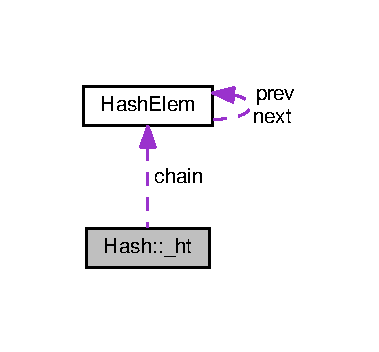
\includegraphics[width=182pt]{structHash_1_1__ht__coll__graph}
\end{center}
\end{figure}
\subsection*{Public Attributes}
\begin{DoxyCompactItemize}
\item 
int {\bfseries count}\hypertarget{structHash_1_1__ht_a0677191178b6c7c5c6c2880f41cf24b1}{}\label{structHash_1_1__ht_a0677191178b6c7c5c6c2880f41cf24b1}

\item 
\hyperlink{structHashElem}{Hash\+Elem} $\ast$ {\bfseries chain}\hypertarget{structHash_1_1__ht_a56fc145e7d38d9440d85ab2ea63a48ac}{}\label{structHash_1_1__ht_a56fc145e7d38d9440d85ab2ea63a48ac}

\end{DoxyCompactItemize}


The documentation for this struct was generated from the following file\+:\begin{DoxyCompactItemize}
\item 
sqlite3.\+c\end{DoxyCompactItemize}

\hypertarget{structAggInfo}{}\section{Agg\+Info Struct Reference}
\label{structAggInfo}\index{Agg\+Info@{Agg\+Info}}


Collaboration diagram for Agg\+Info\+:\nopagebreak
\begin{figure}[H]
\begin{center}
\leavevmode
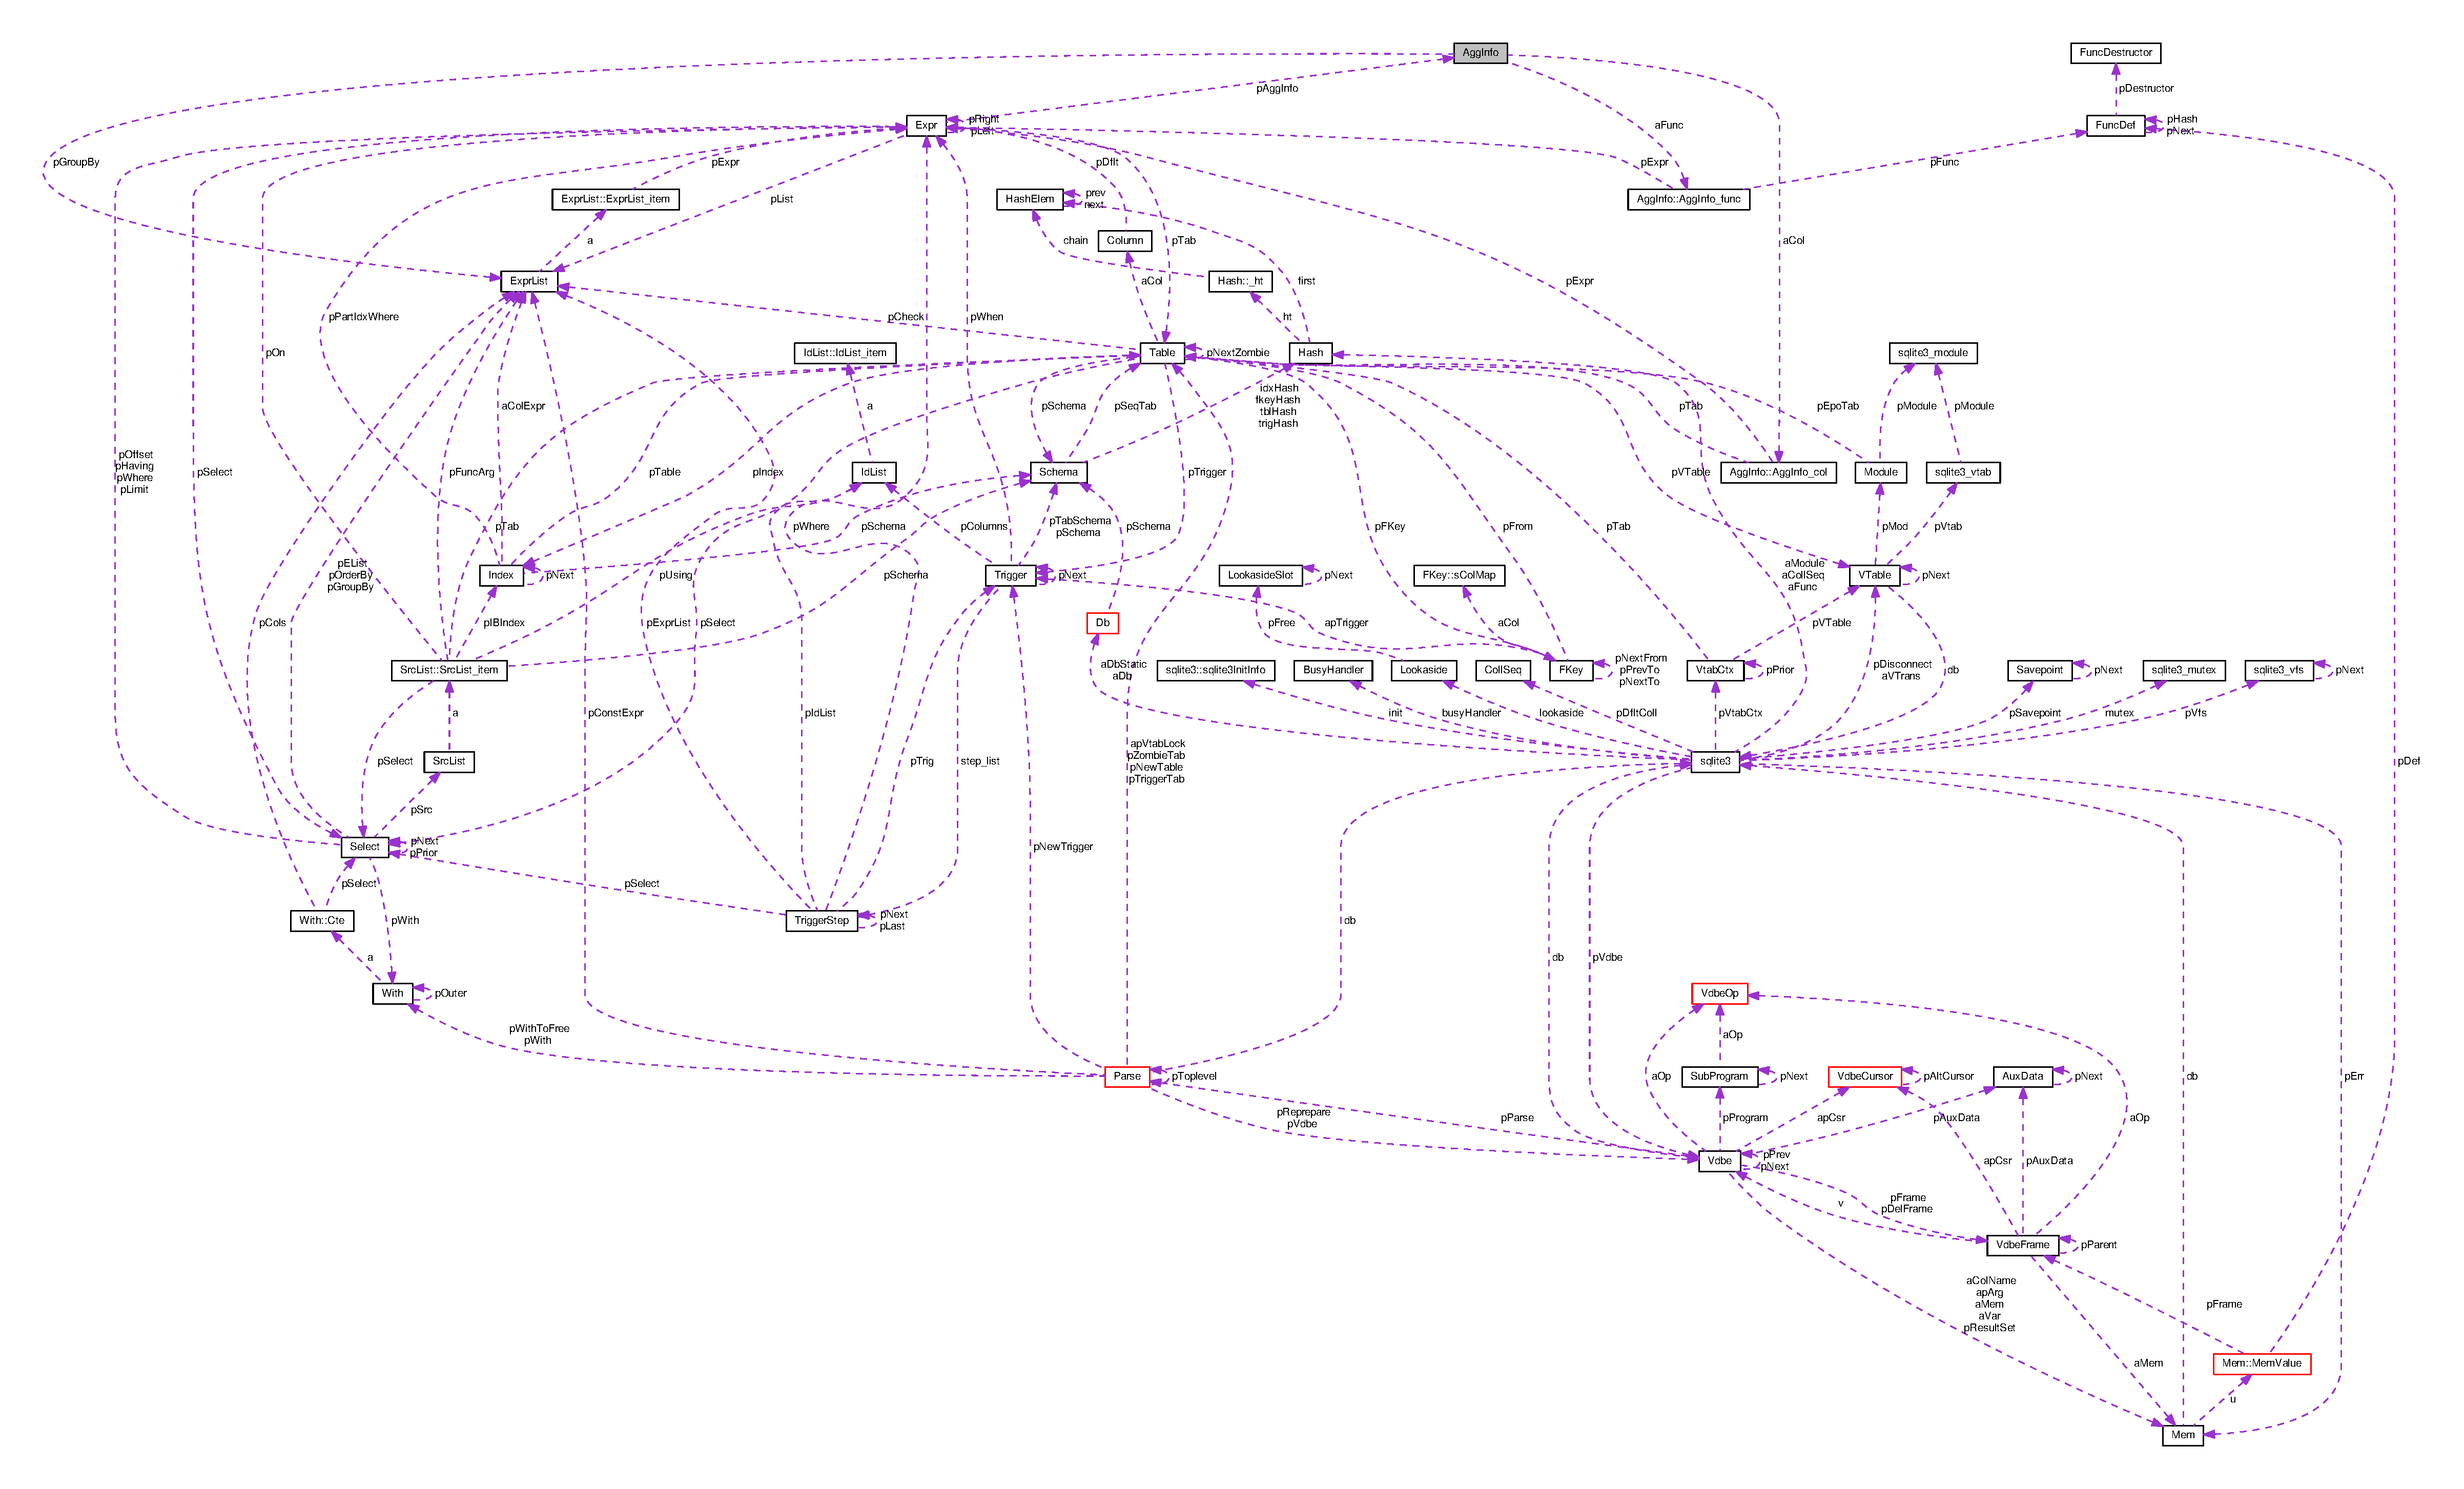
\includegraphics[width=350pt]{structAggInfo__coll__graph}
\end{center}
\end{figure}
\subsection*{Classes}
\begin{DoxyCompactItemize}
\item 
struct \hyperlink{structAggInfo_1_1AggInfo__col}{Agg\+Info\+\_\+col}
\item 
struct \hyperlink{structAggInfo_1_1AggInfo__func}{Agg\+Info\+\_\+func}
\end{DoxyCompactItemize}
\subsection*{Public Attributes}
\begin{DoxyCompactItemize}
\item 
u8 {\bfseries direct\+Mode}\hypertarget{structAggInfo_aaa57d294016ac7e17e7cacaa7b25634e}{}\label{structAggInfo_aaa57d294016ac7e17e7cacaa7b25634e}

\item 
u8 {\bfseries use\+Sorting\+Idx}\hypertarget{structAggInfo_a8173a7ea13c4a12ce4befbcb40719073}{}\label{structAggInfo_a8173a7ea13c4a12ce4befbcb40719073}

\item 
int {\bfseries sorting\+Idx}\hypertarget{structAggInfo_a97ce74f509ca908a616c123e7196797b}{}\label{structAggInfo_a97ce74f509ca908a616c123e7196797b}

\item 
int {\bfseries sorting\+Idx\+P\+Tab}\hypertarget{structAggInfo_a7faac4c3996598960fc46f0c173b244c}{}\label{structAggInfo_a7faac4c3996598960fc46f0c173b244c}

\item 
int {\bfseries n\+Sorting\+Column}\hypertarget{structAggInfo_a89925dccd1a0ec51d2a5a5dbaead66dc}{}\label{structAggInfo_a89925dccd1a0ec51d2a5a5dbaead66dc}

\item 
int {\bfseries mn\+Reg}\hypertarget{structAggInfo_aa9a656c3db8fe0f2905062bbcc55efdc}{}\label{structAggInfo_aa9a656c3db8fe0f2905062bbcc55efdc}

\item 
int {\bfseries mx\+Reg}\hypertarget{structAggInfo_a7aec99396ee3da0bdd985685de1b9da2}{}\label{structAggInfo_a7aec99396ee3da0bdd985685de1b9da2}

\item 
\hyperlink{structExprList}{Expr\+List} $\ast$ {\bfseries p\+Group\+By}\hypertarget{structAggInfo_aa8e942103d224c4db847743670907781}{}\label{structAggInfo_aa8e942103d224c4db847743670907781}

\item 
struct \hyperlink{structAggInfo_1_1AggInfo__col}{Agg\+Info\+::\+Agg\+Info\+\_\+col} $\ast$ {\bfseries a\+Col}\hypertarget{structAggInfo_a52fa1a7eb3145c27be13b2bcccd57d62}{}\label{structAggInfo_a52fa1a7eb3145c27be13b2bcccd57d62}

\item 
int {\bfseries n\+Column}\hypertarget{structAggInfo_a9cbfa5fc33328cf3500426674e036a8b}{}\label{structAggInfo_a9cbfa5fc33328cf3500426674e036a8b}

\item 
int {\bfseries n\+Accumulator}\hypertarget{structAggInfo_ad2251760d95af9024f0a3170405cb53b}{}\label{structAggInfo_ad2251760d95af9024f0a3170405cb53b}

\item 
struct \hyperlink{structAggInfo_1_1AggInfo__func}{Agg\+Info\+::\+Agg\+Info\+\_\+func} $\ast$ {\bfseries a\+Func}\hypertarget{structAggInfo_a4e201acd6a1f8aed360c58e45f47c803}{}\label{structAggInfo_a4e201acd6a1f8aed360c58e45f47c803}

\item 
int {\bfseries n\+Func}\hypertarget{structAggInfo_a5bfde7ca00d28da6edbda523ab038e38}{}\label{structAggInfo_a5bfde7ca00d28da6edbda523ab038e38}

\end{DoxyCompactItemize}


The documentation for this struct was generated from the following file\+:\begin{DoxyCompactItemize}
\item 
sqlite3.\+c\end{DoxyCompactItemize}

\hypertarget{structAggInfo_1_1AggInfo__col}{}\section{Agg\+Info\+:\+:Agg\+Info\+\_\+col Struct Reference}
\label{structAggInfo_1_1AggInfo__col}\index{Agg\+Info\+::\+Agg\+Info\+\_\+col@{Agg\+Info\+::\+Agg\+Info\+\_\+col}}


Collaboration diagram for Agg\+Info\+:\+:Agg\+Info\+\_\+col\+:\nopagebreak
\begin{figure}[H]
\begin{center}
\leavevmode
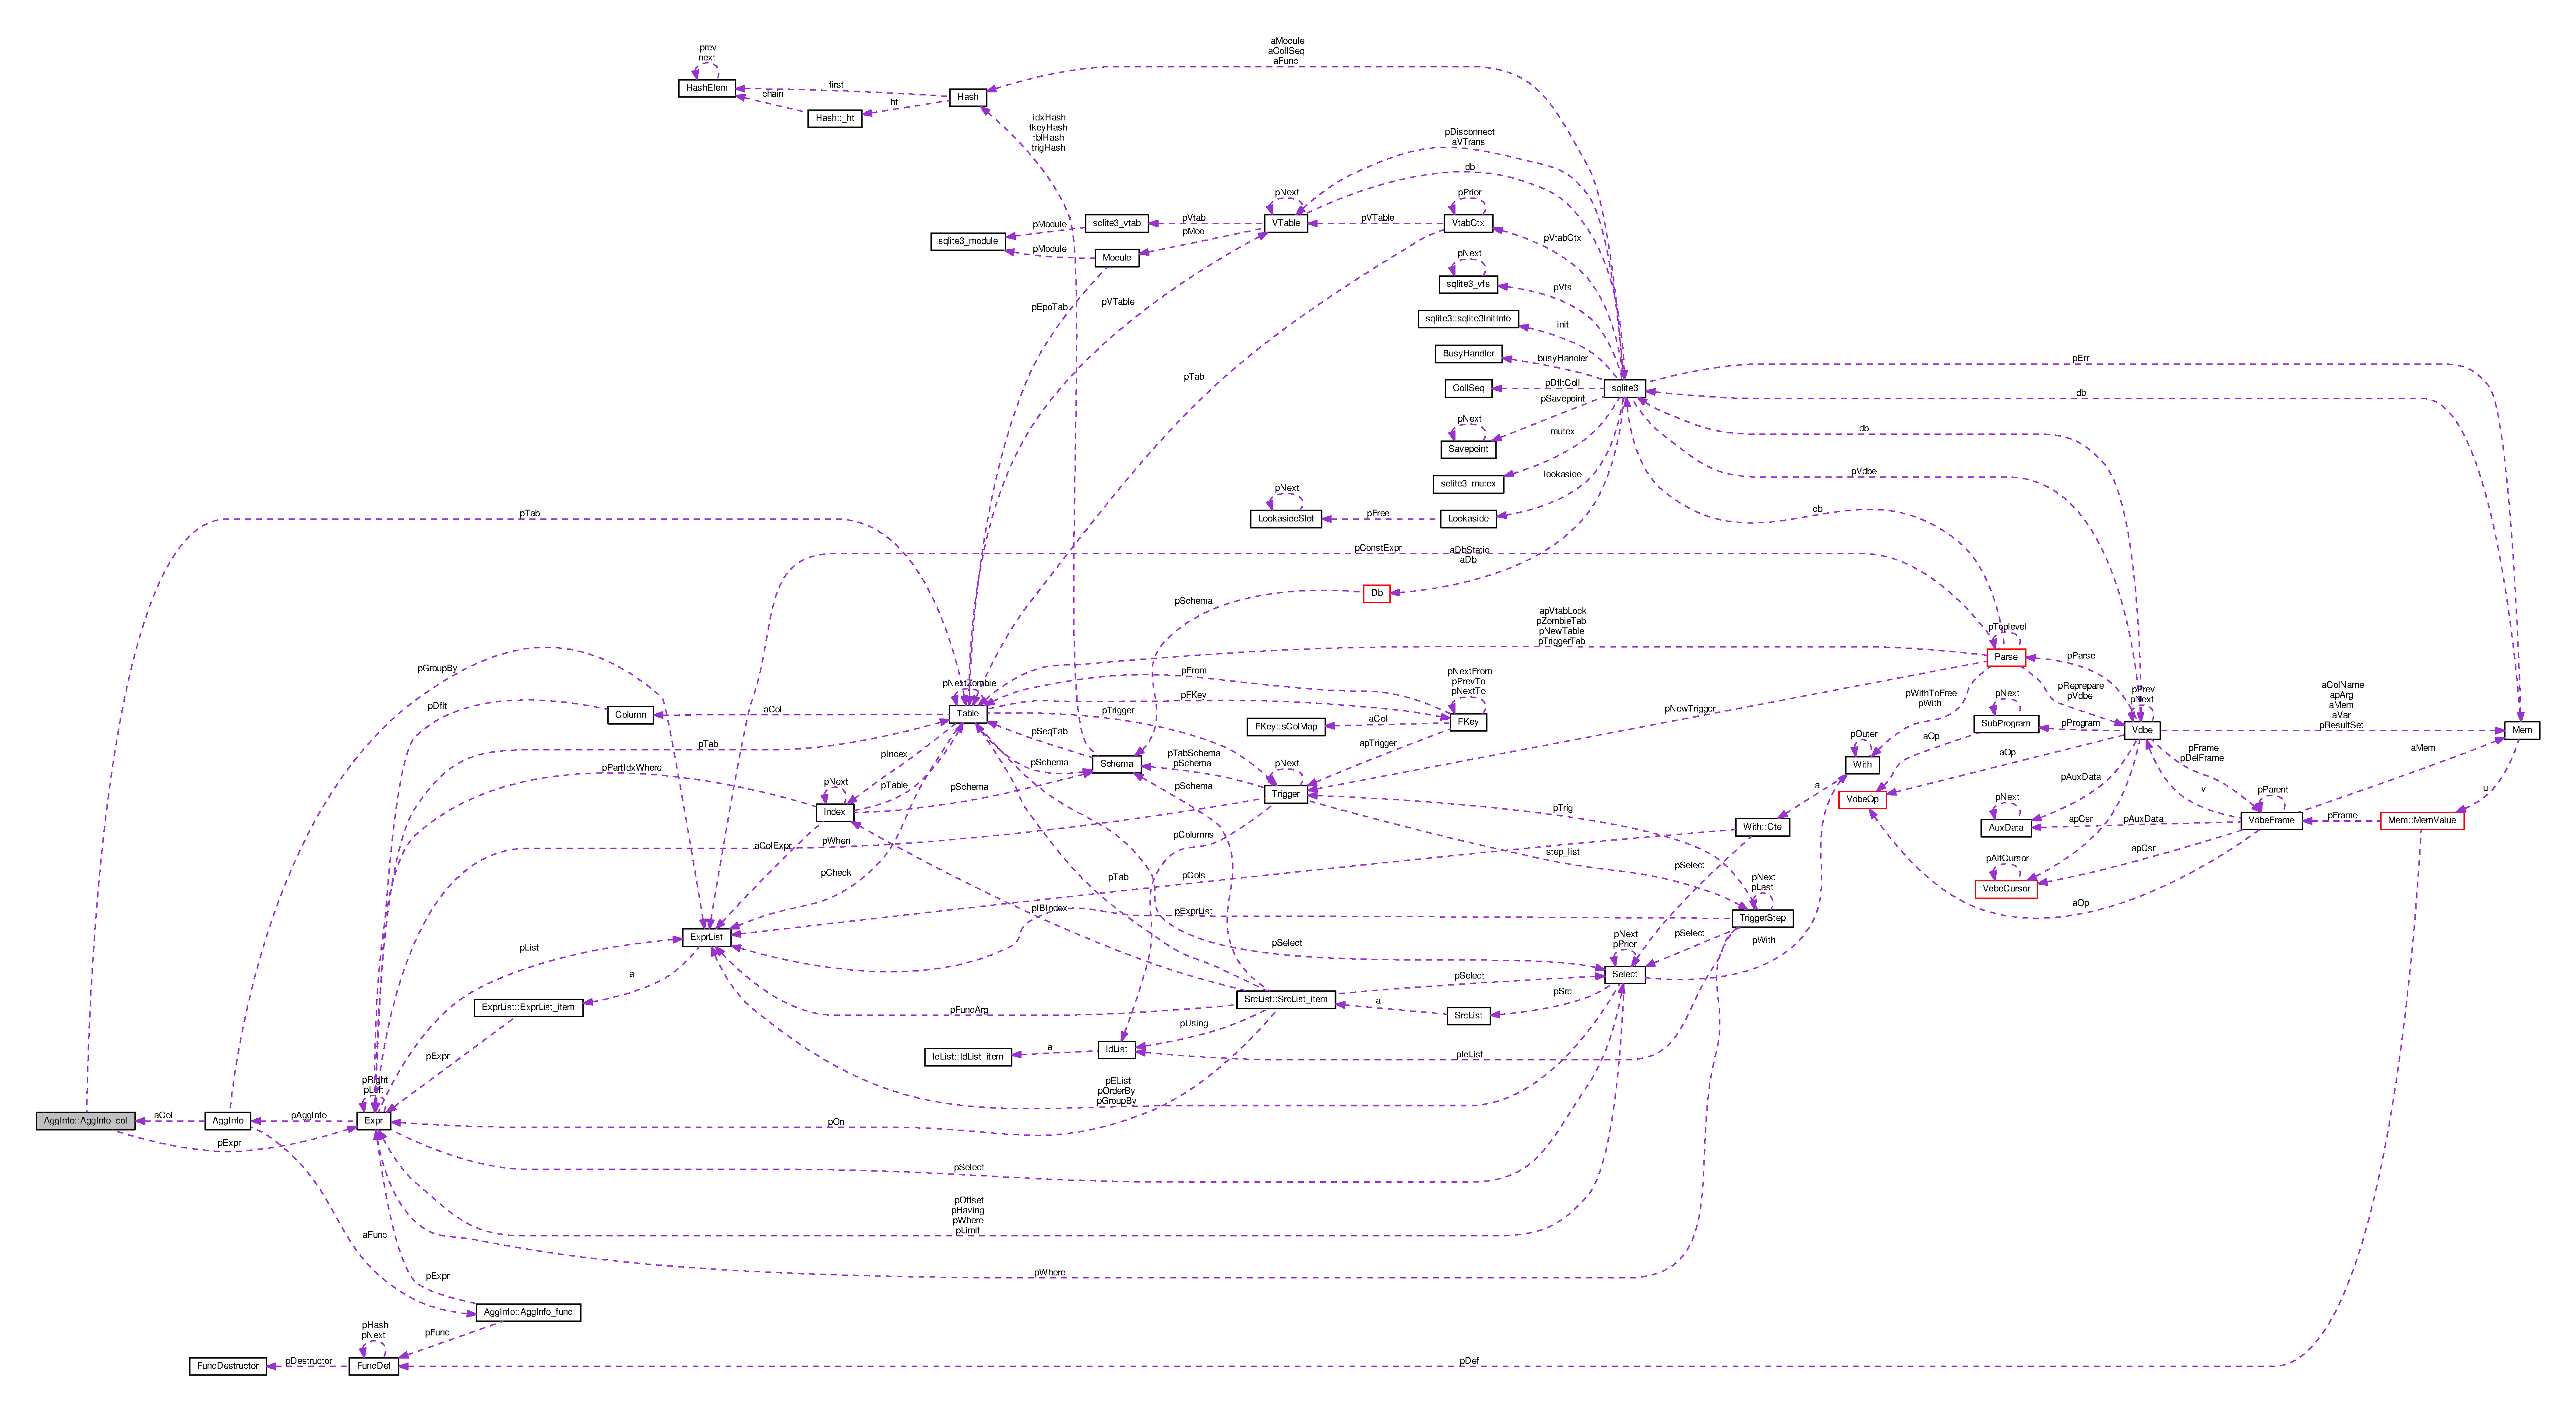
\includegraphics[width=350pt]{structAggInfo_1_1AggInfo__col__coll__graph}
\end{center}
\end{figure}
\subsection*{Public Attributes}
\begin{DoxyCompactItemize}
\item 
\hyperlink{structTable}{Table} $\ast$ {\bfseries p\+Tab}\hypertarget{structAggInfo_1_1AggInfo__col_ad2f2ae137b49e72d28a57accc9d06386}{}\label{structAggInfo_1_1AggInfo__col_ad2f2ae137b49e72d28a57accc9d06386}

\item 
int {\bfseries i\+Table}\hypertarget{structAggInfo_1_1AggInfo__col_ab49aa2fbfc6278c86b64497a6807c113}{}\label{structAggInfo_1_1AggInfo__col_ab49aa2fbfc6278c86b64497a6807c113}

\item 
int {\bfseries i\+Column}\hypertarget{structAggInfo_1_1AggInfo__col_a4cad2ce99ddf7425d358d49e40524f6b}{}\label{structAggInfo_1_1AggInfo__col_a4cad2ce99ddf7425d358d49e40524f6b}

\item 
int {\bfseries i\+Sorter\+Column}\hypertarget{structAggInfo_1_1AggInfo__col_ae3901ad0d5b6d519a7559358f1f7248b}{}\label{structAggInfo_1_1AggInfo__col_ae3901ad0d5b6d519a7559358f1f7248b}

\item 
int {\bfseries i\+Mem}\hypertarget{structAggInfo_1_1AggInfo__col_ae22f3dfc6f9c2dc647be1b9fbd14e896}{}\label{structAggInfo_1_1AggInfo__col_ae22f3dfc6f9c2dc647be1b9fbd14e896}

\item 
\hyperlink{structExpr}{Expr} $\ast$ {\bfseries p\+Expr}\hypertarget{structAggInfo_1_1AggInfo__col_a60f23ec0abfcc88cab7083967a3abd9e}{}\label{structAggInfo_1_1AggInfo__col_a60f23ec0abfcc88cab7083967a3abd9e}

\end{DoxyCompactItemize}


The documentation for this struct was generated from the following file\+:\begin{DoxyCompactItemize}
\item 
sqlite3.\+c\end{DoxyCompactItemize}

\hypertarget{structAggInfo_1_1AggInfo__func}{}\section{Agg\+Info\+:\+:Agg\+Info\+\_\+func Struct Reference}
\label{structAggInfo_1_1AggInfo__func}\index{Agg\+Info\+::\+Agg\+Info\+\_\+func@{Agg\+Info\+::\+Agg\+Info\+\_\+func}}


Collaboration diagram for Agg\+Info\+:\+:Agg\+Info\+\_\+func\+:
% FIG 0
\subsection*{Public Attributes}
\begin{DoxyCompactItemize}
\item 
\hyperlink{structExpr}{Expr} $\ast$ {\bfseries p\+Expr}\hypertarget{structAggInfo_1_1AggInfo__func_a7b92e1c42e60d44e28ebf695316f4018}{}\label{structAggInfo_1_1AggInfo__func_a7b92e1c42e60d44e28ebf695316f4018}

\item 
\hyperlink{structFuncDef}{Func\+Def} $\ast$ {\bfseries p\+Func}\hypertarget{structAggInfo_1_1AggInfo__func_a840478e8ec53cefa57b50228f6fdafe4}{}\label{structAggInfo_1_1AggInfo__func_a840478e8ec53cefa57b50228f6fdafe4}

\item 
int {\bfseries i\+Mem}\hypertarget{structAggInfo_1_1AggInfo__func_a41a8da36555c37fffc65f1acead49a4f}{}\label{structAggInfo_1_1AggInfo__func_a41a8da36555c37fffc65f1acead49a4f}

\item 
int {\bfseries i\+Distinct}\hypertarget{structAggInfo_1_1AggInfo__func_a4a82635b0116eb44ec8ca9e47cc509d9}{}\label{structAggInfo_1_1AggInfo__func_a4a82635b0116eb44ec8ca9e47cc509d9}

\end{DoxyCompactItemize}


The documentation for this struct was generated from the following file\+:\begin{DoxyCompactItemize}
\item 
sqlite3.\+c\end{DoxyCompactItemize}

\hypertarget{structanalysisInfo}{}\section{analysis\+Info Struct Reference}
\label{structanalysisInfo}\index{analysis\+Info@{analysis\+Info}}


Collaboration diagram for analysis\+Info\+:\nopagebreak
\begin{figure}[H]
\begin{center}
\leavevmode
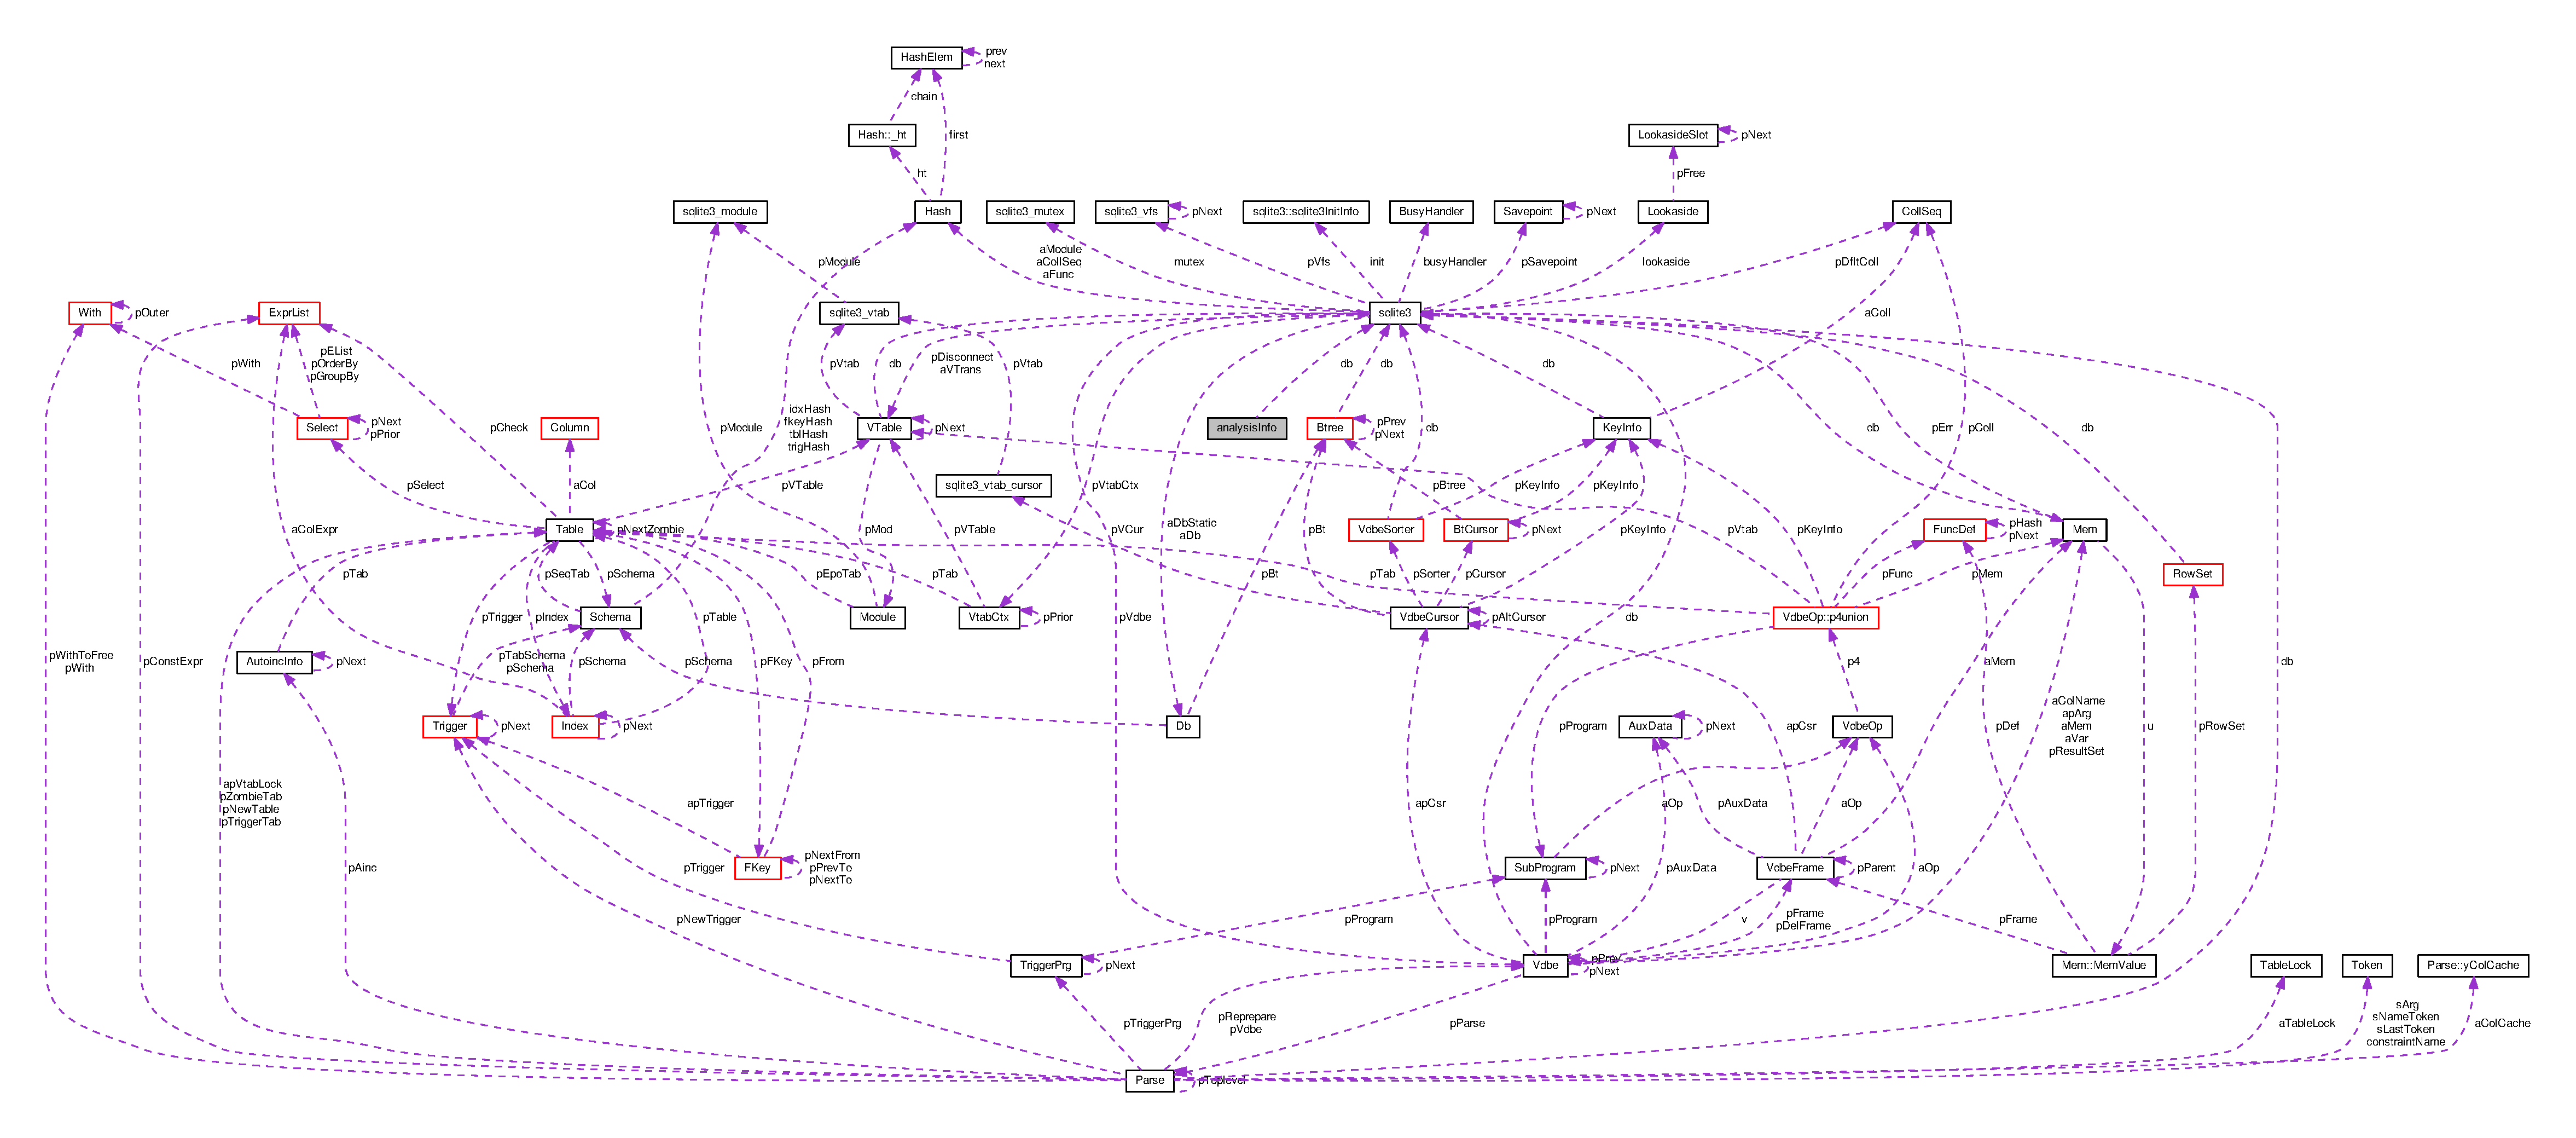
\includegraphics[width=350pt]{structanalysisInfo__coll__graph}
\end{center}
\end{figure}
\subsection*{Public Attributes}
\begin{DoxyCompactItemize}
\item 
\hyperlink{structsqlite3}{sqlite3} $\ast$ {\bfseries db}\hypertarget{structanalysisInfo_a13108eadc55ffe73a8825fb91cc0f9b5}{}\label{structanalysisInfo_a13108eadc55ffe73a8825fb91cc0f9b5}

\item 
const char $\ast$ {\bfseries z\+Database}\hypertarget{structanalysisInfo_accbe3c1f5613ffa13b9578e58a5d850a}{}\label{structanalysisInfo_accbe3c1f5613ffa13b9578e58a5d850a}

\end{DoxyCompactItemize}


The documentation for this struct was generated from the following file\+:\begin{DoxyCompactItemize}
\item 
sqlite3.\+c\end{DoxyCompactItemize}

\hypertarget{structAuthContext}{}\section{Auth\+Context Struct Reference}
\label{structAuthContext}\index{Auth\+Context@{Auth\+Context}}


Collaboration diagram for Auth\+Context\+:\nopagebreak
\begin{figure}[H]
\begin{center}
\leavevmode
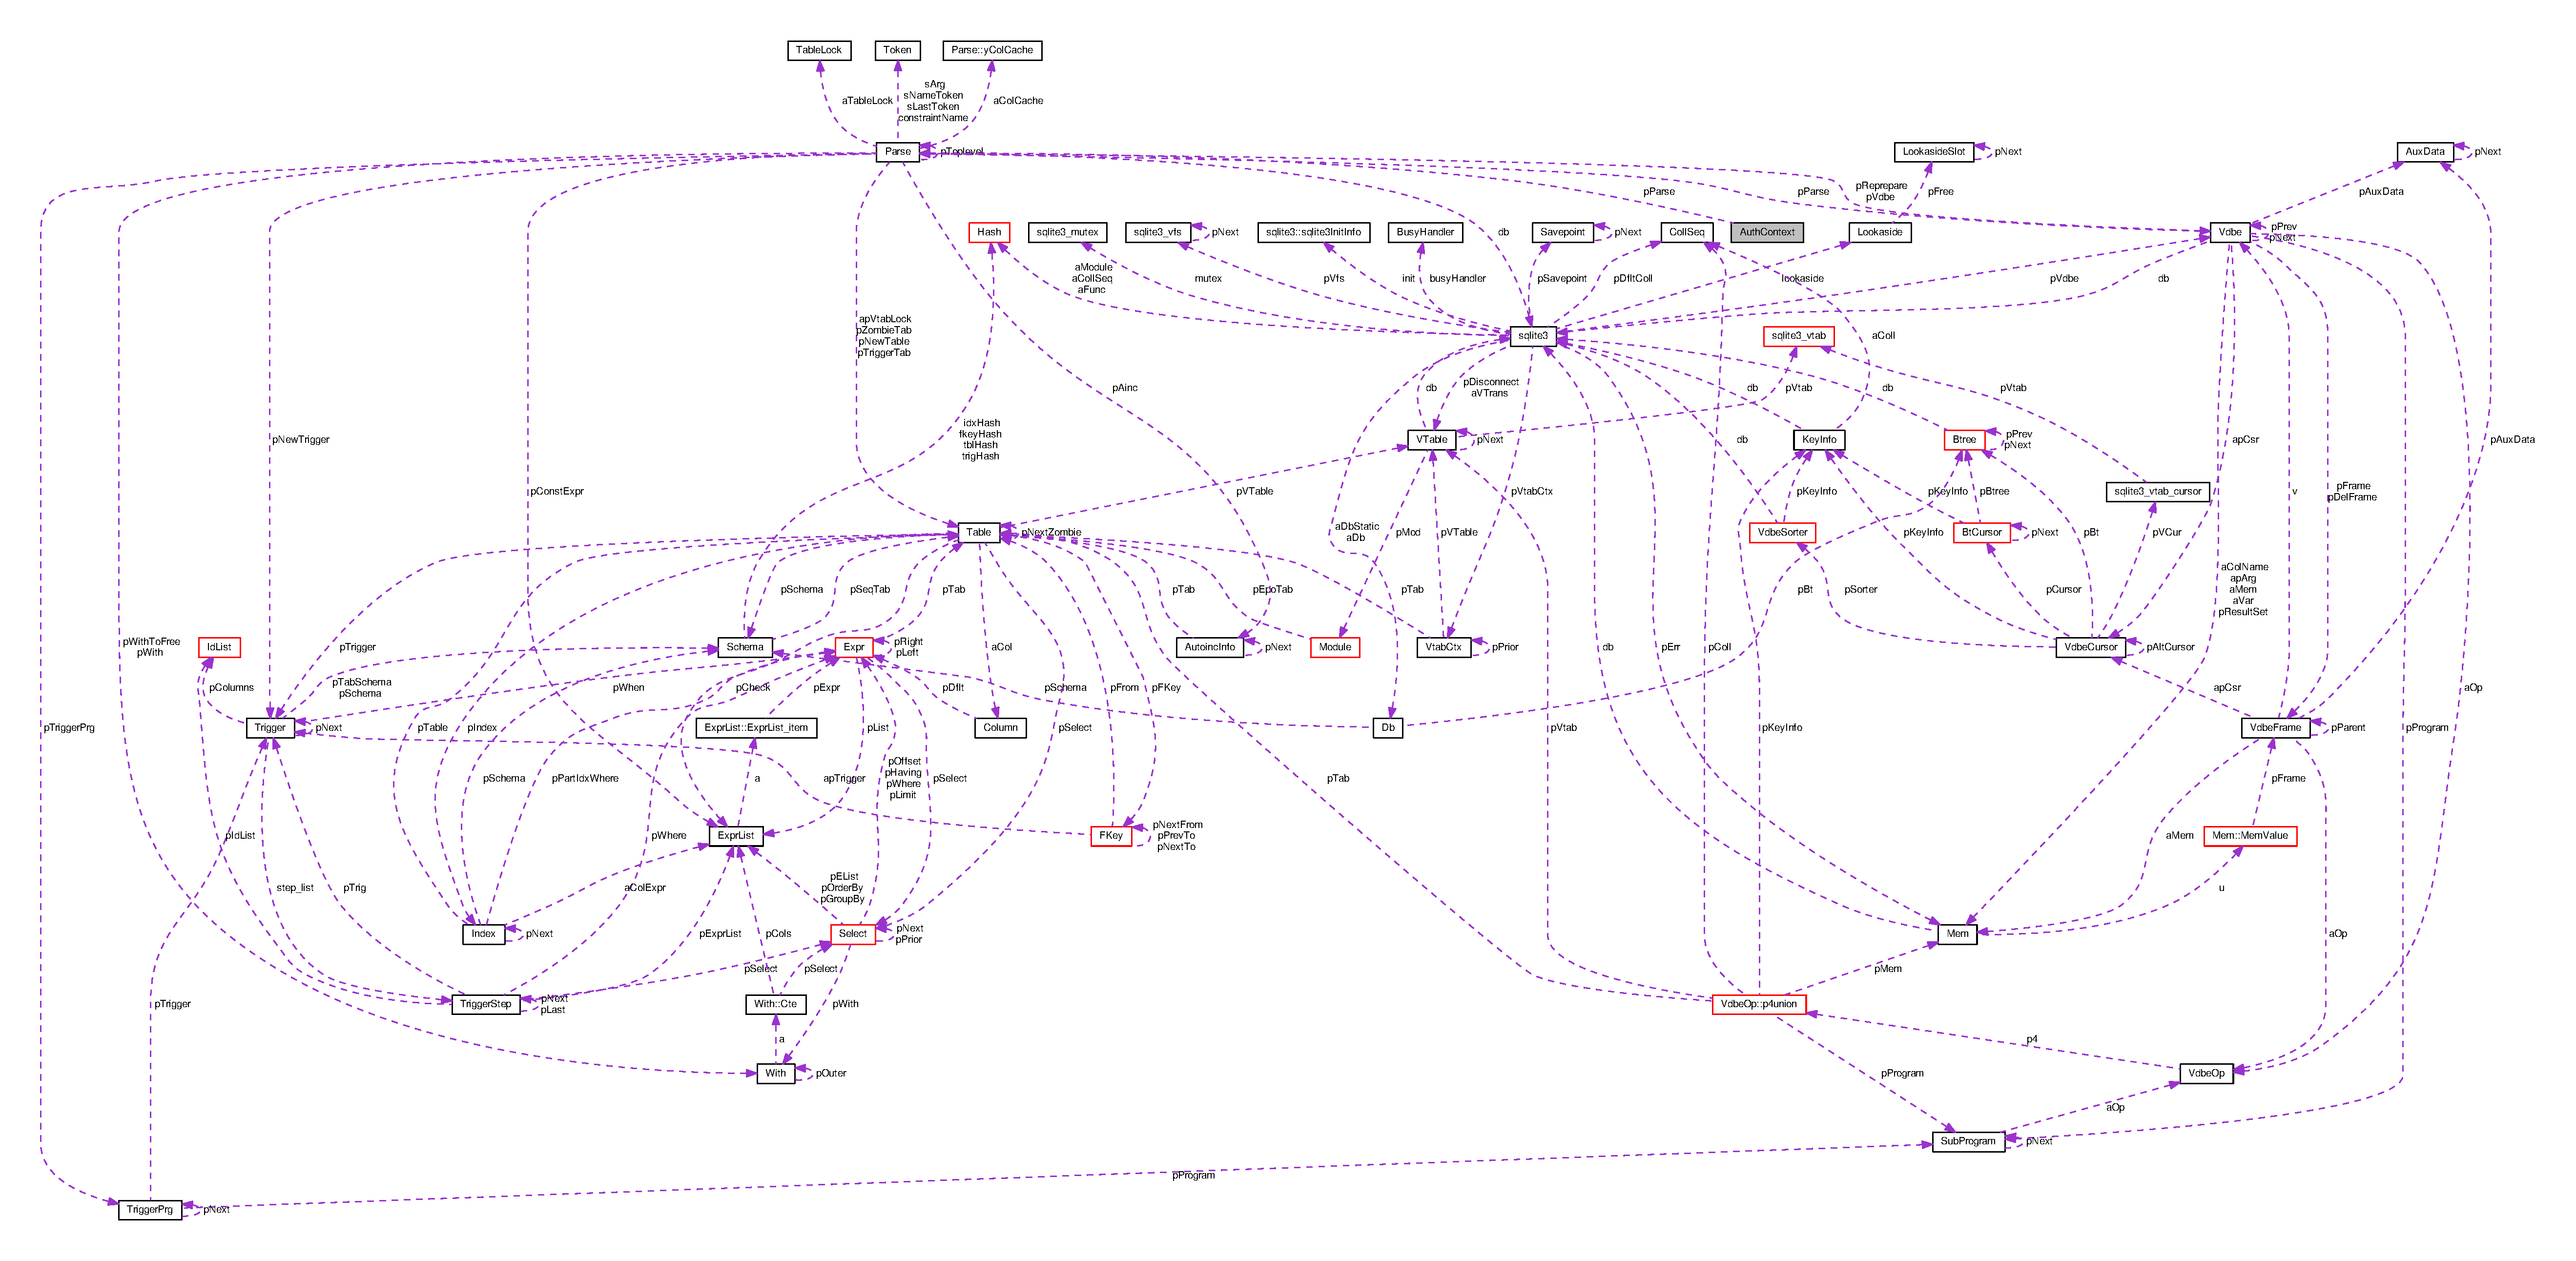
\includegraphics[width=350pt]{structAuthContext__coll__graph}
\end{center}
\end{figure}
\subsection*{Public Attributes}
\begin{DoxyCompactItemize}
\item 
const char $\ast$ {\bfseries z\+Auth\+Context}\hypertarget{structAuthContext_a1b095b152b72326476ac3f7edcaee78a}{}\label{structAuthContext_a1b095b152b72326476ac3f7edcaee78a}

\item 
\hyperlink{structParse}{Parse} $\ast$ {\bfseries p\+Parse}\hypertarget{structAuthContext_a8df2931d8f4facf59073c92315b00bfa}{}\label{structAuthContext_a8df2931d8f4facf59073c92315b00bfa}

\end{DoxyCompactItemize}


The documentation for this struct was generated from the following file\+:\begin{DoxyCompactItemize}
\item 
sqlite3.\+c\end{DoxyCompactItemize}

\hypertarget{structAutoincInfo}{}\section{Autoinc\+Info Struct Reference}
\label{structAutoincInfo}\index{Autoinc\+Info@{Autoinc\+Info}}


Collaboration diagram for Autoinc\+Info\+:\nopagebreak
\begin{figure}[H]
\begin{center}
\leavevmode
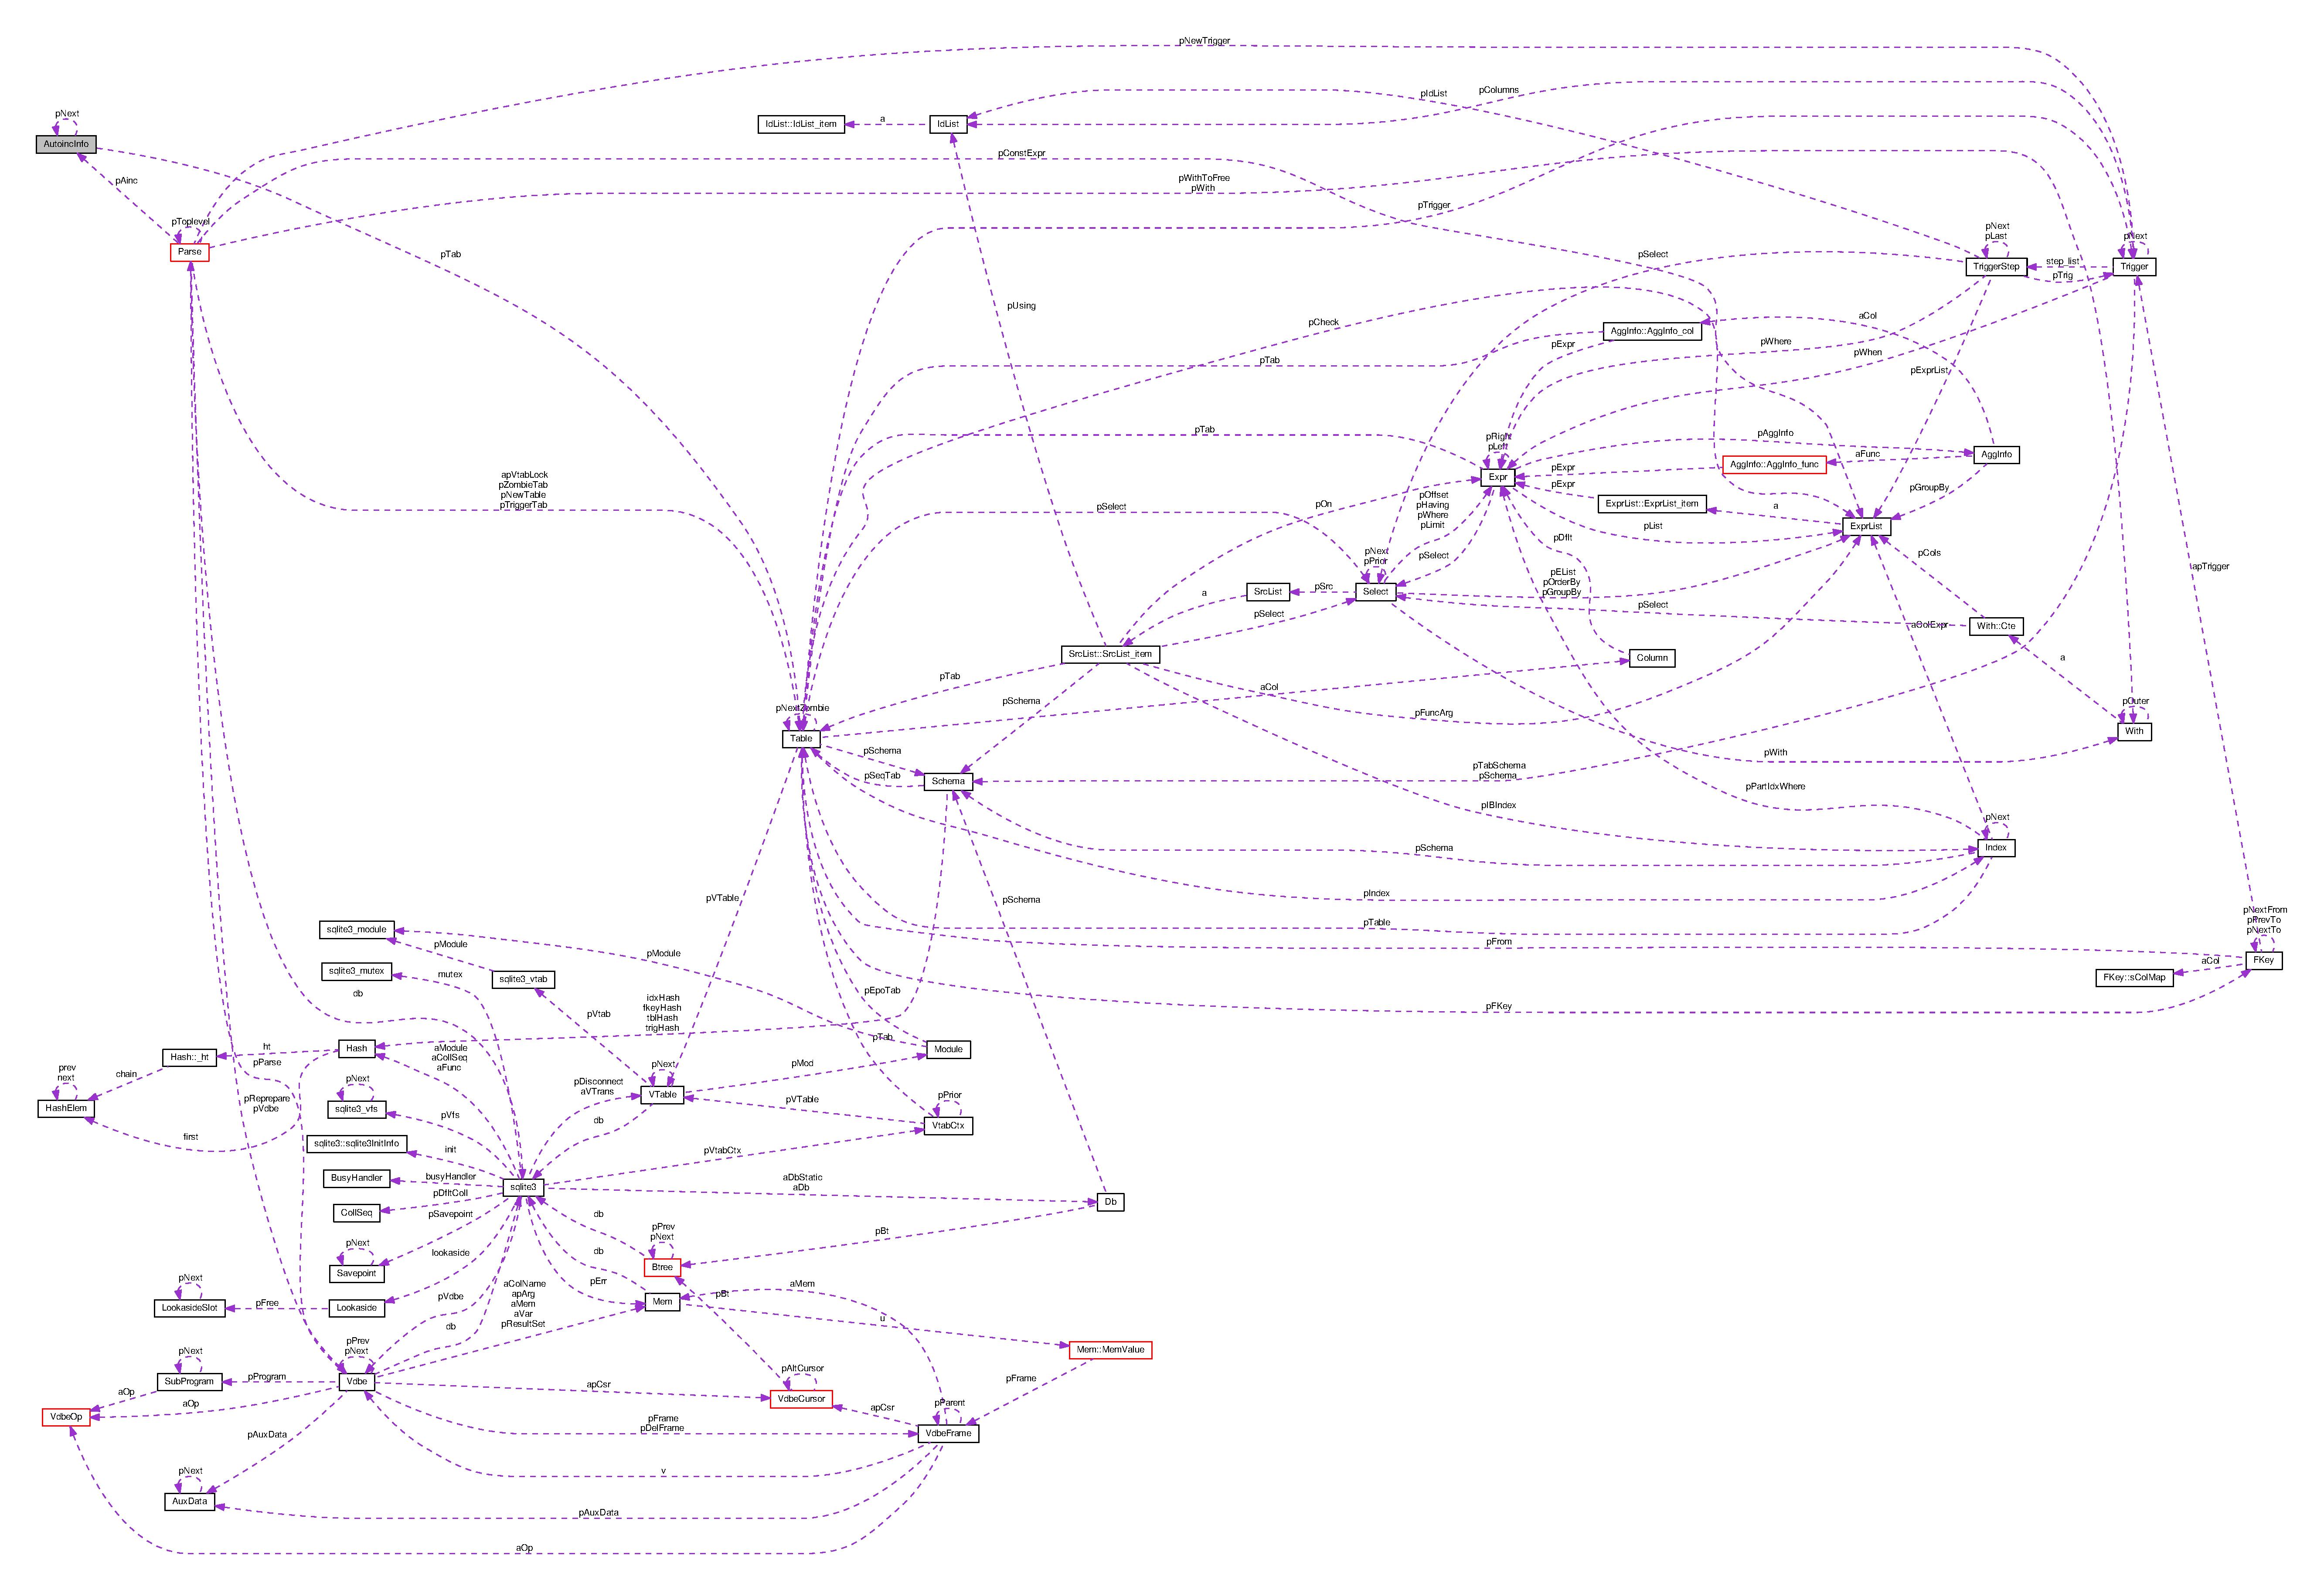
\includegraphics[width=350pt]{structAutoincInfo__coll__graph}
\end{center}
\end{figure}
\subsection*{Public Attributes}
\begin{DoxyCompactItemize}
\item 
\hyperlink{structAutoincInfo}{Autoinc\+Info} $\ast$ {\bfseries p\+Next}\hypertarget{structAutoincInfo_aa77fb076beea013c25df4e49dba4b6f6}{}\label{structAutoincInfo_aa77fb076beea013c25df4e49dba4b6f6}

\item 
\hyperlink{structTable}{Table} $\ast$ {\bfseries p\+Tab}\hypertarget{structAutoincInfo_a0cf785b0cbaddb4215a8408f8e13075e}{}\label{structAutoincInfo_a0cf785b0cbaddb4215a8408f8e13075e}

\item 
int {\bfseries i\+Db}\hypertarget{structAutoincInfo_ae7234e0916b11ef97377bdfd6c7c4568}{}\label{structAutoincInfo_ae7234e0916b11ef97377bdfd6c7c4568}

\item 
int {\bfseries reg\+Ctr}\hypertarget{structAutoincInfo_af180977ee7dcc8cab862185692f57cc5}{}\label{structAutoincInfo_af180977ee7dcc8cab862185692f57cc5}

\end{DoxyCompactItemize}


The documentation for this struct was generated from the following file\+:\begin{DoxyCompactItemize}
\item 
sqlite3.\+c\end{DoxyCompactItemize}

\hypertarget{structAuxData}{}\section{Aux\+Data Struct Reference}
\label{structAuxData}\index{Aux\+Data@{Aux\+Data}}


Collaboration diagram for Aux\+Data\+:\nopagebreak
\begin{figure}[H]
\begin{center}
\leavevmode
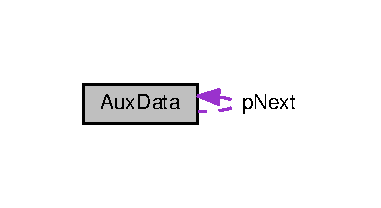
\includegraphics[width=183pt]{structAuxData__coll__graph}
\end{center}
\end{figure}
\subsection*{Public Attributes}
\begin{DoxyCompactItemize}
\item 
int {\bfseries i\+Op}\hypertarget{structAuxData_aaa45d5e867df81e58b886f4fe355364f}{}\label{structAuxData_aaa45d5e867df81e58b886f4fe355364f}

\item 
int {\bfseries i\+Arg}\hypertarget{structAuxData_aa0f1b63cbd4f0cf17c82d9ed17bbdc01}{}\label{structAuxData_aa0f1b63cbd4f0cf17c82d9ed17bbdc01}

\item 
void $\ast$ {\bfseries p\+Aux}\hypertarget{structAuxData_a3867fd2bd1f3795b14e858daa6754825}{}\label{structAuxData_a3867fd2bd1f3795b14e858daa6754825}

\item 
void($\ast$ {\bfseries x\+Delete} )(void $\ast$)\hypertarget{structAuxData_ae2c39019bc42d3650d21d9b4f8692400}{}\label{structAuxData_ae2c39019bc42d3650d21d9b4f8692400}

\item 
\hyperlink{structAuxData}{Aux\+Data} $\ast$ {\bfseries p\+Next}\hypertarget{structAuxData_af63a17e0ce6af2de969caccb25ef3945}{}\label{structAuxData_af63a17e0ce6af2de969caccb25ef3945}

\end{DoxyCompactItemize}


The documentation for this struct was generated from the following file\+:\begin{DoxyCompactItemize}
\item 
sqlite3.\+c\end{DoxyCompactItemize}

\hypertarget{structBitvec}{}\section{Bitvec Struct Reference}
\label{structBitvec}\index{Bitvec@{Bitvec}}


Collaboration diagram for Bitvec\+:
% FIG 0
\subsection*{Public Attributes}
\begin{DoxyCompactItemize}
\item 
u32 {\bfseries i\+Size}\hypertarget{structBitvec_ab36df8ece98aee080bae6de28c237de8}{}\label{structBitvec_ab36df8ece98aee080bae6de28c237de8}

\item 
u32 {\bfseries n\+Set}\hypertarget{structBitvec_ad6811debae9b972f2d94d667e994e3f6}{}\label{structBitvec_ad6811debae9b972f2d94d667e994e3f6}

\item 
u32 {\bfseries i\+Divisor}\hypertarget{structBitvec_a22cdb23eb424e07b6ce922de018a83d9}{}\label{structBitvec_a22cdb23eb424e07b6ce922de018a83d9}

\item 
\begin{tabbing}
xx\=xx\=xx\=xx\=xx\=xx\=xx\=xx\=xx\=\kill
union \{\\
\>BITVEC\_TELEM {\bfseries aBitmap} \mbox{[}BITVEC\_NELEM\mbox{]}\\
\>u32 {\bfseries aHash} \mbox{[}BITVEC\_NINT\mbox{]}\\
\>\hyperlink{structBitvec}{Bitvec} $\ast$ {\bfseries apSub} \mbox{[}BITVEC\_NPTR\mbox{]}\\
\} {\bfseries u}\hypertarget{structBitvec_a580a692d761462ea1576d1fdcb6d97fa}{}\label{structBitvec_a580a692d761462ea1576d1fdcb6d97fa}
\\

\end{tabbing}\end{DoxyCompactItemize}


The documentation for this struct was generated from the following file\+:\begin{DoxyCompactItemize}
\item 
sqlite3.\+c\end{DoxyCompactItemize}

\hypertarget{structBtCursor}{}\section{Bt\+Cursor Struct Reference}
\label{structBtCursor}\index{Bt\+Cursor@{Bt\+Cursor}}


Collaboration diagram for Bt\+Cursor\+:
% FIG 0
\subsection*{Public Attributes}
\begin{DoxyCompactItemize}
\item 
\hyperlink{structBtree}{Btree} $\ast$ {\bfseries p\+Btree}\hypertarget{structBtCursor_a2ad810542eaf99c9919c585624bead6f}{}\label{structBtCursor_a2ad810542eaf99c9919c585624bead6f}

\item 
\hyperlink{structBtShared}{Bt\+Shared} $\ast$ {\bfseries p\+Bt}\hypertarget{structBtCursor_a61c245712549192f7644e5ac23c00b74}{}\label{structBtCursor_a61c245712549192f7644e5ac23c00b74}

\item 
\hyperlink{structBtCursor}{Bt\+Cursor} $\ast$ {\bfseries p\+Next}\hypertarget{structBtCursor_ad2f8fe3aa7d3fa3309692b3e8a8c2395}{}\label{structBtCursor_ad2f8fe3aa7d3fa3309692b3e8a8c2395}

\item 
Pgno $\ast$ {\bfseries a\+Overflow}\hypertarget{structBtCursor_ae2dbcc15e63d349774a7ad6caef4d096}{}\label{structBtCursor_ae2dbcc15e63d349774a7ad6caef4d096}

\item 
\hyperlink{structCellInfo}{Cell\+Info} {\bfseries info}\hypertarget{structBtCursor_a9934b348c6e9f4808d8f98ea78788fbe}{}\label{structBtCursor_a9934b348c6e9f4808d8f98ea78788fbe}

\item 
i64 {\bfseries n\+Key}\hypertarget{structBtCursor_a23f6a271258c109aaeda0ba19e808f92}{}\label{structBtCursor_a23f6a271258c109aaeda0ba19e808f92}

\item 
void $\ast$ {\bfseries p\+Key}\hypertarget{structBtCursor_a3c979824f27f63678d7a2b02311bc330}{}\label{structBtCursor_a3c979824f27f63678d7a2b02311bc330}

\item 
Pgno {\bfseries pgno\+Root}\hypertarget{structBtCursor_a0b038f63a5b1b9df0b892e0773ffdd29}{}\label{structBtCursor_a0b038f63a5b1b9df0b892e0773ffdd29}

\item 
int {\bfseries n\+Ovfl\+Alloc}\hypertarget{structBtCursor_a114e01e9e27ae7640796fa6258bda937}{}\label{structBtCursor_a114e01e9e27ae7640796fa6258bda937}

\item 
int {\bfseries skip\+Next}\hypertarget{structBtCursor_ab1dfdbd6c9ec6cdb21cdb5deaa6d5ecb}{}\label{structBtCursor_ab1dfdbd6c9ec6cdb21cdb5deaa6d5ecb}

\item 
u8 {\bfseries cur\+Flags}\hypertarget{structBtCursor_ab120d81b3550eabce37f377cbdae8836}{}\label{structBtCursor_ab120d81b3550eabce37f377cbdae8836}

\item 
u8 {\bfseries cur\+Pager\+Flags}\hypertarget{structBtCursor_aff2ef1cec10fbfc0c2d35277b5ee4432}{}\label{structBtCursor_aff2ef1cec10fbfc0c2d35277b5ee4432}

\item 
u8 {\bfseries e\+State}\hypertarget{structBtCursor_a30ab5e7109965b34a08562a7b7e6de15}{}\label{structBtCursor_a30ab5e7109965b34a08562a7b7e6de15}

\item 
u8 {\bfseries hints}\hypertarget{structBtCursor_ad8c66c31cf1a2c2181d61a64ca951a8a}{}\label{structBtCursor_ad8c66c31cf1a2c2181d61a64ca951a8a}

\item 
i8 {\bfseries i\+Page}\hypertarget{structBtCursor_adfe516b0ae2c030f5963fda944bf6d8e}{}\label{structBtCursor_adfe516b0ae2c030f5963fda944bf6d8e}

\item 
u8 {\bfseries cur\+Int\+Key}\hypertarget{structBtCursor_a37db7ea50e0f355ea6a3d8d3213722c3}{}\label{structBtCursor_a37db7ea50e0f355ea6a3d8d3213722c3}

\item 
struct \hyperlink{structKeyInfo}{Key\+Info} $\ast$ {\bfseries p\+Key\+Info}\hypertarget{structBtCursor_ad2360bda13f959ed70672eb421fdb5ec}{}\label{structBtCursor_ad2360bda13f959ed70672eb421fdb5ec}

\item 
void $\ast$ {\bfseries padding1}\hypertarget{structBtCursor_ac4321376ea6d26d2aa7f7cc905e09310}{}\label{structBtCursor_ac4321376ea6d26d2aa7f7cc905e09310}

\item 
u16 {\bfseries ai\+Idx} \mbox{[}B\+T\+C\+U\+R\+S\+O\+R\+\_\+\+M\+A\+X\+\_\+\+D\+E\+P\+TH\mbox{]}\hypertarget{structBtCursor_a037a739198de5bee22ca203d34e90af1}{}\label{structBtCursor_a037a739198de5bee22ca203d34e90af1}

\item 
\hyperlink{structMemPage}{Mem\+Page} $\ast$ {\bfseries ap\+Page} \mbox{[}B\+T\+C\+U\+R\+S\+O\+R\+\_\+\+M\+A\+X\+\_\+\+D\+E\+P\+TH\mbox{]}\hypertarget{structBtCursor_ad3414d944f9578e86e26c6158f92096b}{}\label{structBtCursor_ad3414d944f9578e86e26c6158f92096b}

\end{DoxyCompactItemize}


The documentation for this struct was generated from the following file\+:\begin{DoxyCompactItemize}
\item 
sqlite3.\+c\end{DoxyCompactItemize}

\hypertarget{structBtLock}{}\section{Bt\+Lock Struct Reference}
\label{structBtLock}\index{Bt\+Lock@{Bt\+Lock}}


Collaboration diagram for Bt\+Lock\+:\nopagebreak
\begin{figure}[H]
\begin{center}
\leavevmode
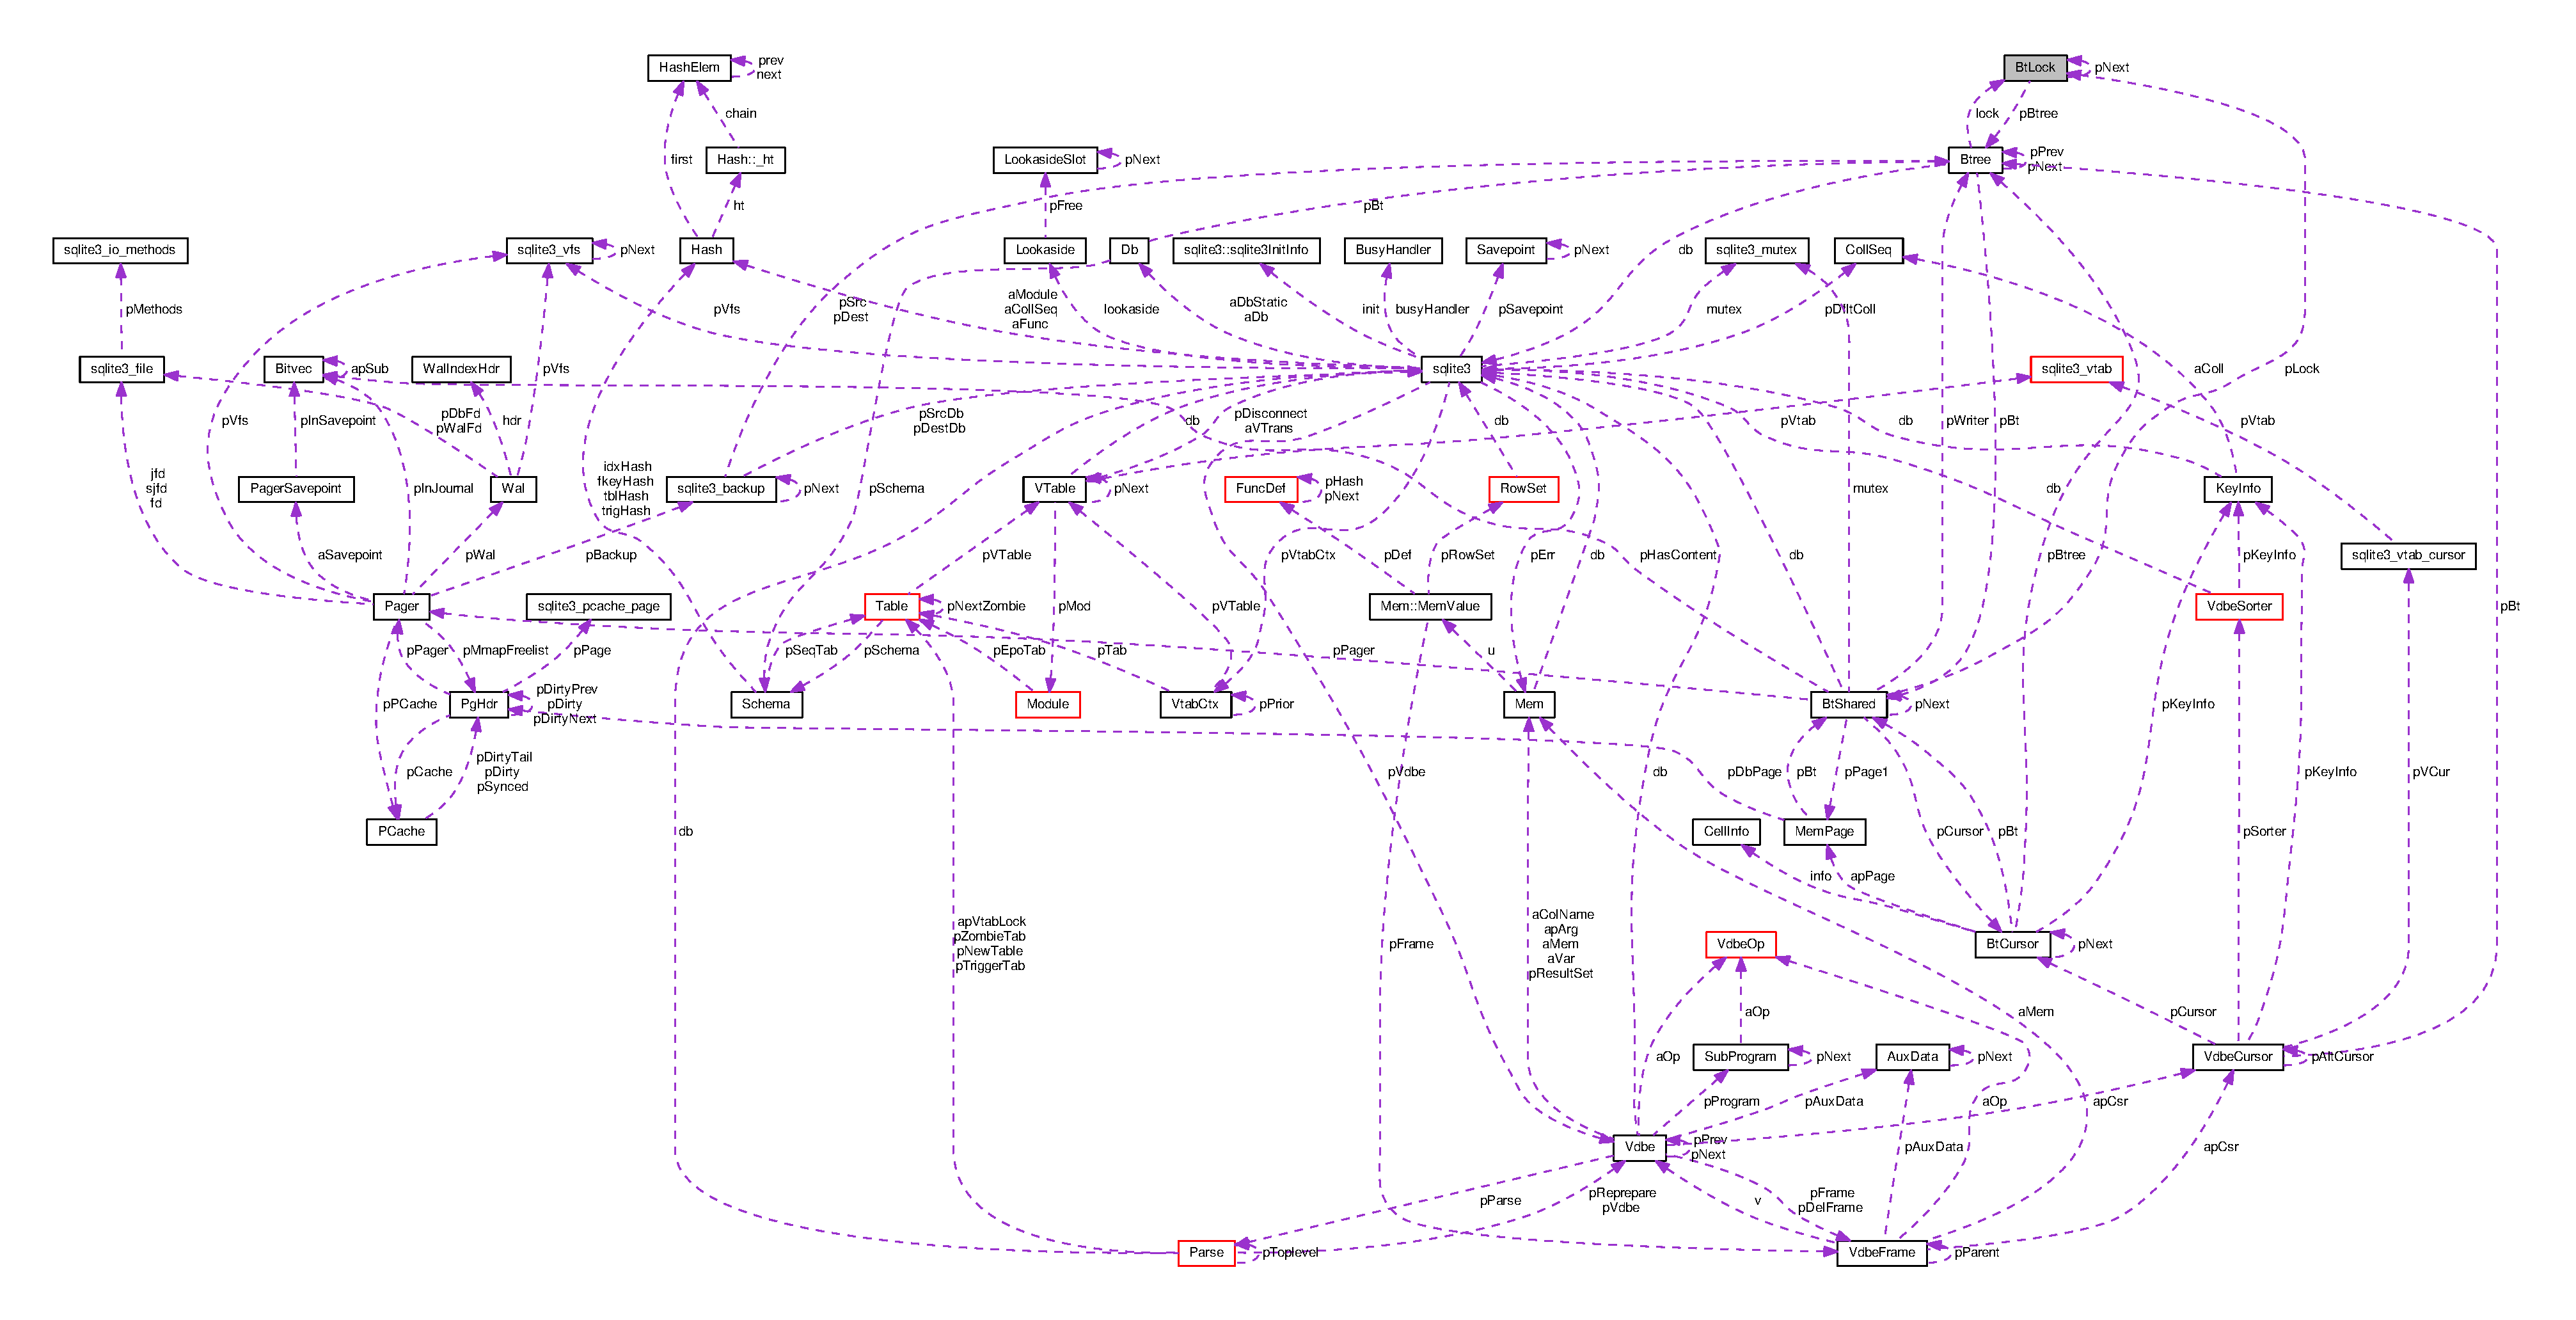
\includegraphics[width=350pt]{structBtLock__coll__graph}
\end{center}
\end{figure}
\subsection*{Public Attributes}
\begin{DoxyCompactItemize}
\item 
\hyperlink{structBtree}{Btree} $\ast$ {\bfseries p\+Btree}\hypertarget{structBtLock_ab9125b8e79d480b75f3af21cb2ab55c7}{}\label{structBtLock_ab9125b8e79d480b75f3af21cb2ab55c7}

\item 
Pgno {\bfseries i\+Table}\hypertarget{structBtLock_a822efcf018d6c8eb343341cde5df980d}{}\label{structBtLock_a822efcf018d6c8eb343341cde5df980d}

\item 
u8 {\bfseries e\+Lock}\hypertarget{structBtLock_abe07b71018ee423e0d94b5cdba044b5c}{}\label{structBtLock_abe07b71018ee423e0d94b5cdba044b5c}

\item 
\hyperlink{structBtLock}{Bt\+Lock} $\ast$ {\bfseries p\+Next}\hypertarget{structBtLock_ad42de86209c7aab43604c52a549b7bca}{}\label{structBtLock_ad42de86209c7aab43604c52a549b7bca}

\end{DoxyCompactItemize}


The documentation for this struct was generated from the following file\+:\begin{DoxyCompactItemize}
\item 
sqlite3.\+c\end{DoxyCompactItemize}

\hypertarget{structBtree}{}\section{Btree Struct Reference}
\label{structBtree}\index{Btree@{Btree}}


Collaboration diagram for Btree\+:\nopagebreak
\begin{figure}[H]
\begin{center}
\leavevmode
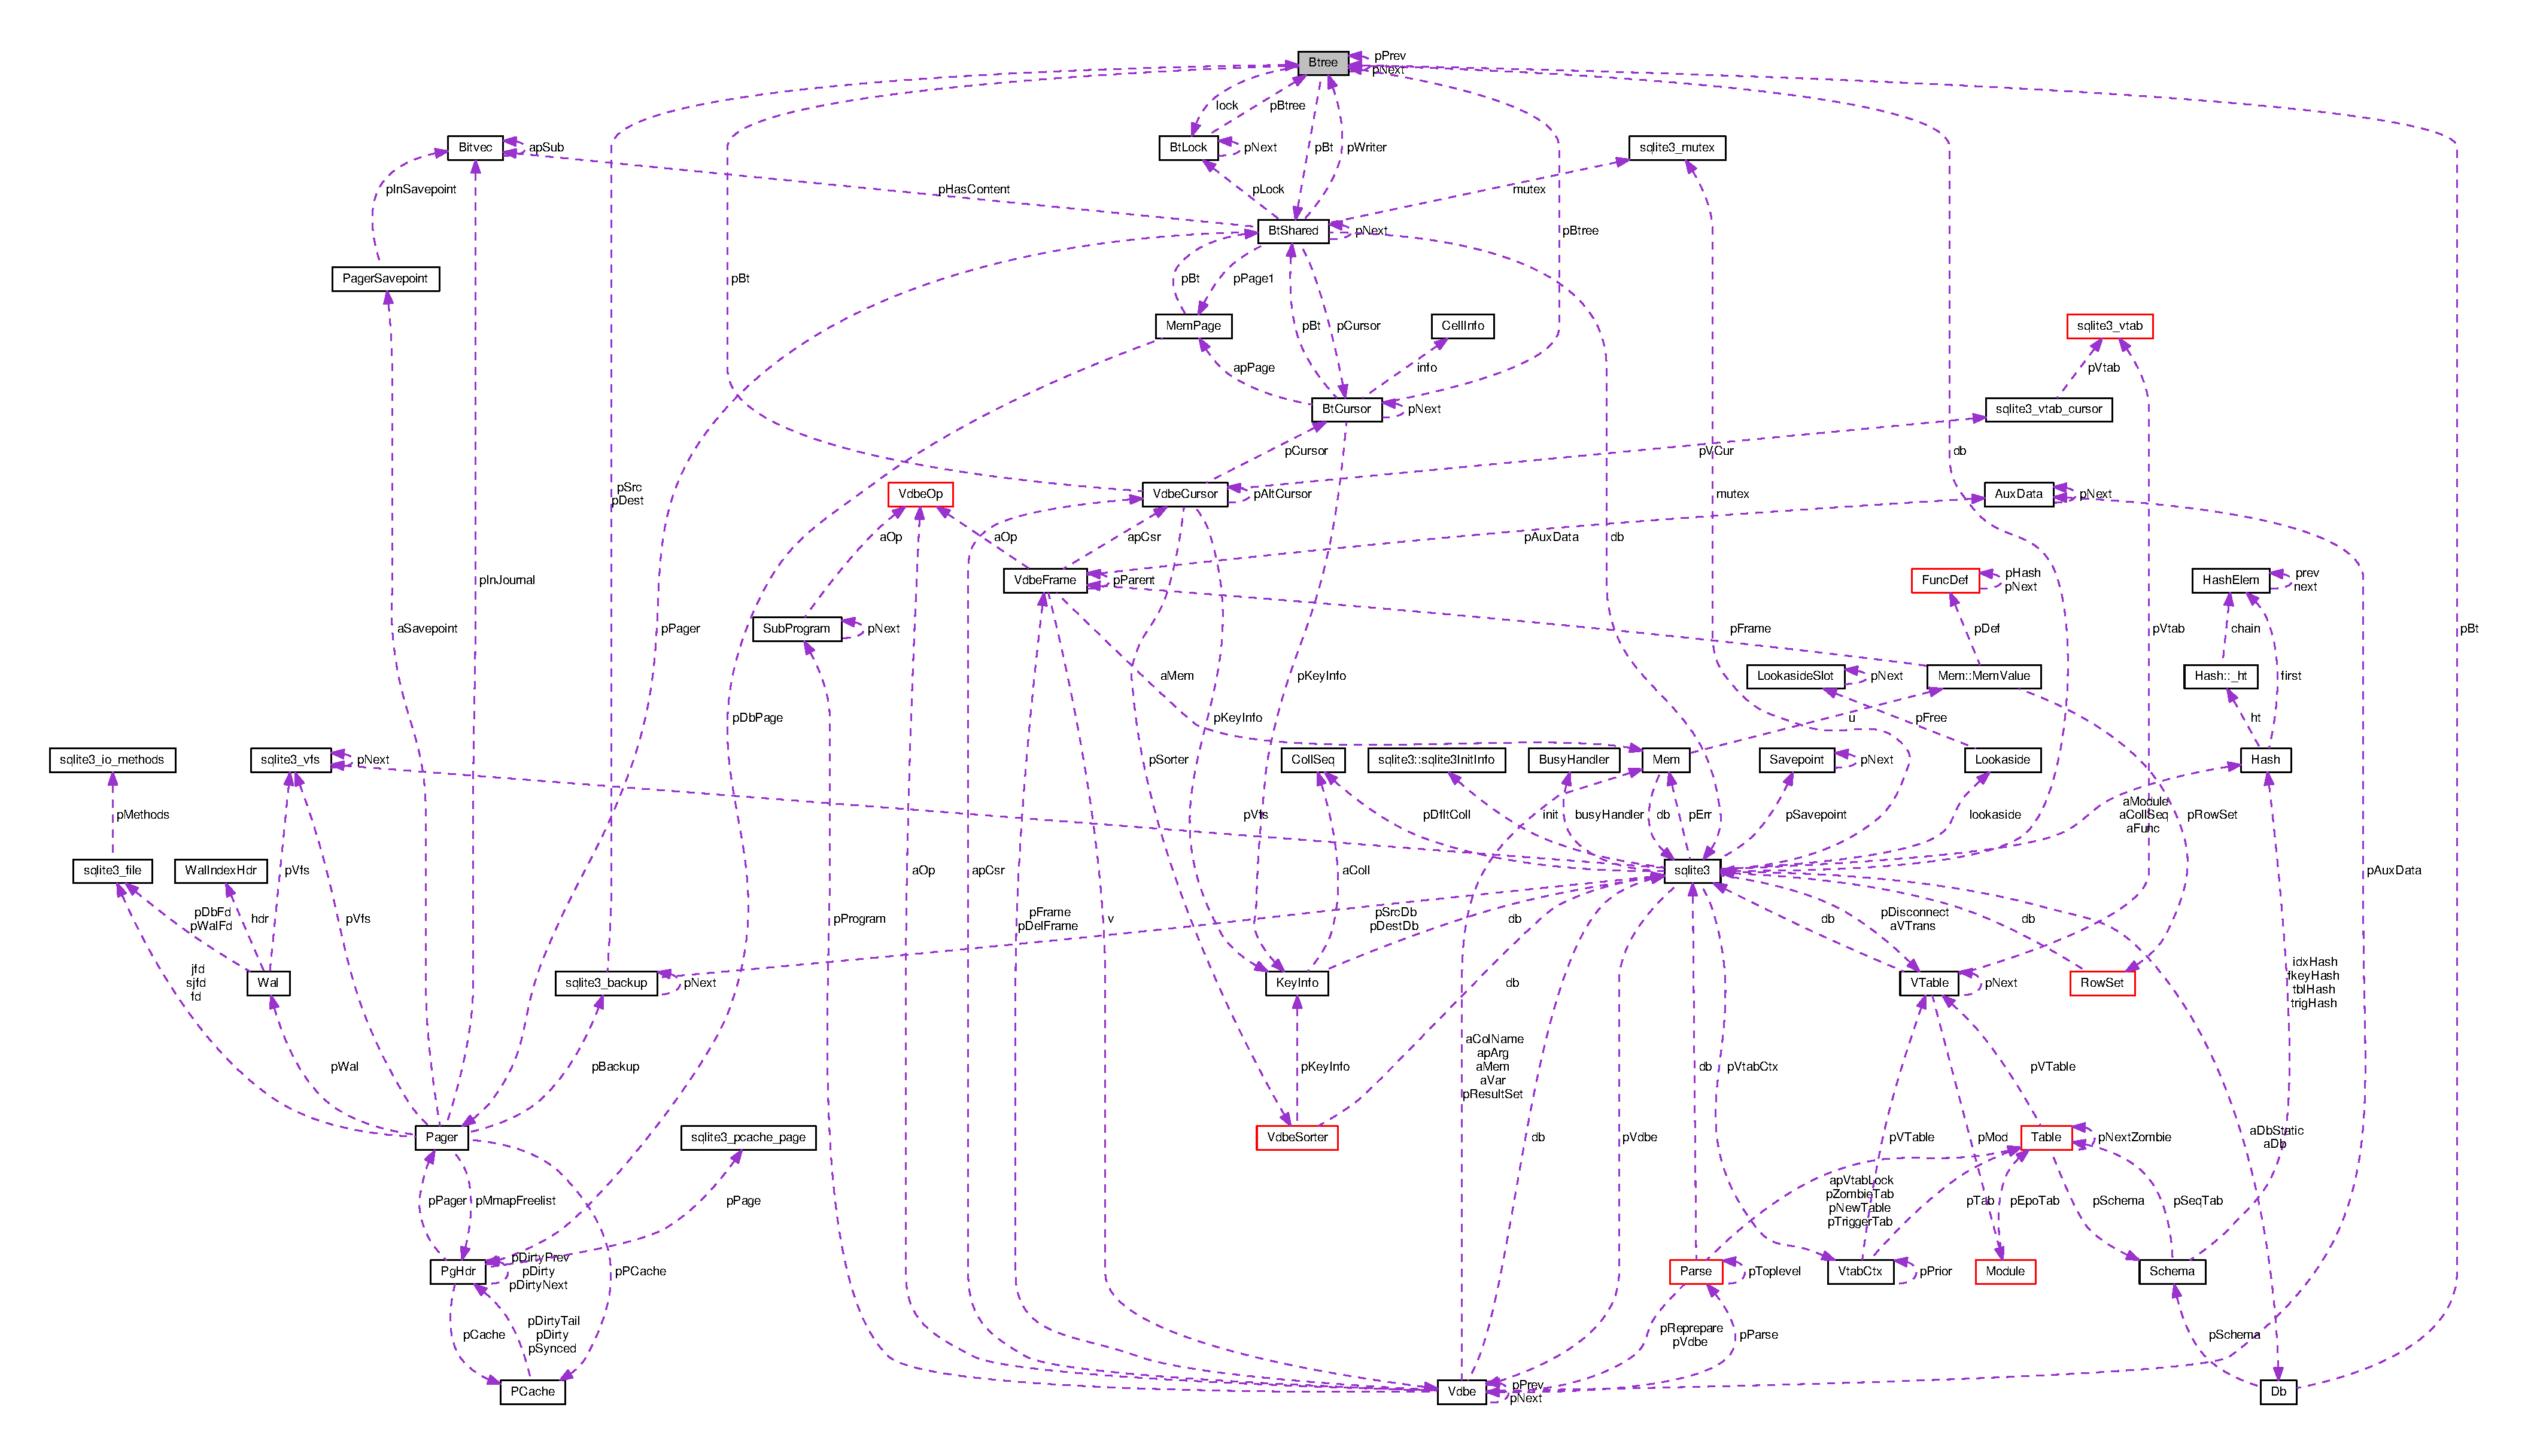
\includegraphics[width=350pt]{structBtree__coll__graph}
\end{center}
\end{figure}
\subsection*{Public Attributes}
\begin{DoxyCompactItemize}
\item 
\hyperlink{structsqlite3}{sqlite3} $\ast$ {\bfseries db}\hypertarget{structBtree_a2b3cfec48b6e9fcfd641d433816ae5c3}{}\label{structBtree_a2b3cfec48b6e9fcfd641d433816ae5c3}

\item 
\hyperlink{structBtShared}{Bt\+Shared} $\ast$ {\bfseries p\+Bt}\hypertarget{structBtree_a63bab5d744d48d14368af048dddf2f20}{}\label{structBtree_a63bab5d744d48d14368af048dddf2f20}

\item 
u8 {\bfseries in\+Trans}\hypertarget{structBtree_a50007448960c05dfd1fdc7db3e277685}{}\label{structBtree_a50007448960c05dfd1fdc7db3e277685}

\item 
u8 {\bfseries sharable}\hypertarget{structBtree_a114f157127c76a1fbad8292e4b39c4dd}{}\label{structBtree_a114f157127c76a1fbad8292e4b39c4dd}

\item 
u8 {\bfseries locked}\hypertarget{structBtree_a16fc8292bae9a66cfec03f6cb82d06a8}{}\label{structBtree_a16fc8292bae9a66cfec03f6cb82d06a8}

\item 
u8 {\bfseries has\+Incrblob\+Cur}\hypertarget{structBtree_a247c6bd4123c5d53ebb96bd879047e25}{}\label{structBtree_a247c6bd4123c5d53ebb96bd879047e25}

\item 
int {\bfseries want\+To\+Lock}\hypertarget{structBtree_a97368ea300f0b74b8e80ea07da0cea2a}{}\label{structBtree_a97368ea300f0b74b8e80ea07da0cea2a}

\item 
int {\bfseries n\+Backup}\hypertarget{structBtree_a7a3e7cf38bc9c3021a9e270a54ecfb1e}{}\label{structBtree_a7a3e7cf38bc9c3021a9e270a54ecfb1e}

\item 
u32 {\bfseries i\+Data\+Version}\hypertarget{structBtree_a333e24a5c4340e94bad7aa13aa36ae31}{}\label{structBtree_a333e24a5c4340e94bad7aa13aa36ae31}

\item 
\hyperlink{structBtree}{Btree} $\ast$ {\bfseries p\+Next}\hypertarget{structBtree_a9e6d2ca44c10ed8ef0be004225a74ef5}{}\label{structBtree_a9e6d2ca44c10ed8ef0be004225a74ef5}

\item 
\hyperlink{structBtree}{Btree} $\ast$ {\bfseries p\+Prev}\hypertarget{structBtree_a0423f1c55c1fe6812161a49bb2bf604f}{}\label{structBtree_a0423f1c55c1fe6812161a49bb2bf604f}

\item 
\hyperlink{structBtLock}{Bt\+Lock} {\bfseries lock}\hypertarget{structBtree_a943ed8799c9943f753a88cf44f1632dc}{}\label{structBtree_a943ed8799c9943f753a88cf44f1632dc}

\end{DoxyCompactItemize}


The documentation for this struct was generated from the following file\+:\begin{DoxyCompactItemize}
\item 
sqlite3.\+c\end{DoxyCompactItemize}

\hypertarget{structBtreePayload}{}\section{Btree\+Payload Struct Reference}
\label{structBtreePayload}\index{Btree\+Payload@{Btree\+Payload}}
\subsection*{Public Attributes}
\begin{DoxyCompactItemize}
\item 
const void $\ast$ {\bfseries p\+Key}\hypertarget{structBtreePayload_a8122b6f070adf318fe4d5131cf877ef3}{}\label{structBtreePayload_a8122b6f070adf318fe4d5131cf877ef3}

\item 
sqlite3\+\_\+int64 {\bfseries n\+Key}\hypertarget{structBtreePayload_ab47f827f8ad41b179f25693d867795a5}{}\label{structBtreePayload_ab47f827f8ad41b179f25693d867795a5}

\item 
const void $\ast$ {\bfseries p\+Data}\hypertarget{structBtreePayload_af45874b2d6119c220280e4ebcd917662}{}\label{structBtreePayload_af45874b2d6119c220280e4ebcd917662}

\item 
int {\bfseries n\+Data}\hypertarget{structBtreePayload_a515a370eeb96e103dd716fa5149f2787}{}\label{structBtreePayload_a515a370eeb96e103dd716fa5149f2787}

\item 
int {\bfseries n\+Zero}\hypertarget{structBtreePayload_ab9c8ecd88e88f7374f95c8b4bccdf946}{}\label{structBtreePayload_ab9c8ecd88e88f7374f95c8b4bccdf946}

\end{DoxyCompactItemize}


The documentation for this struct was generated from the following file\+:\begin{DoxyCompactItemize}
\item 
sqlite3.\+c\end{DoxyCompactItemize}

\hypertarget{structBtShared}{}\section{Bt\+Shared Struct Reference}
\label{structBtShared}\index{Bt\+Shared@{Bt\+Shared}}


Collaboration diagram for Bt\+Shared\+:\nopagebreak
\begin{figure}[H]
\begin{center}
\leavevmode
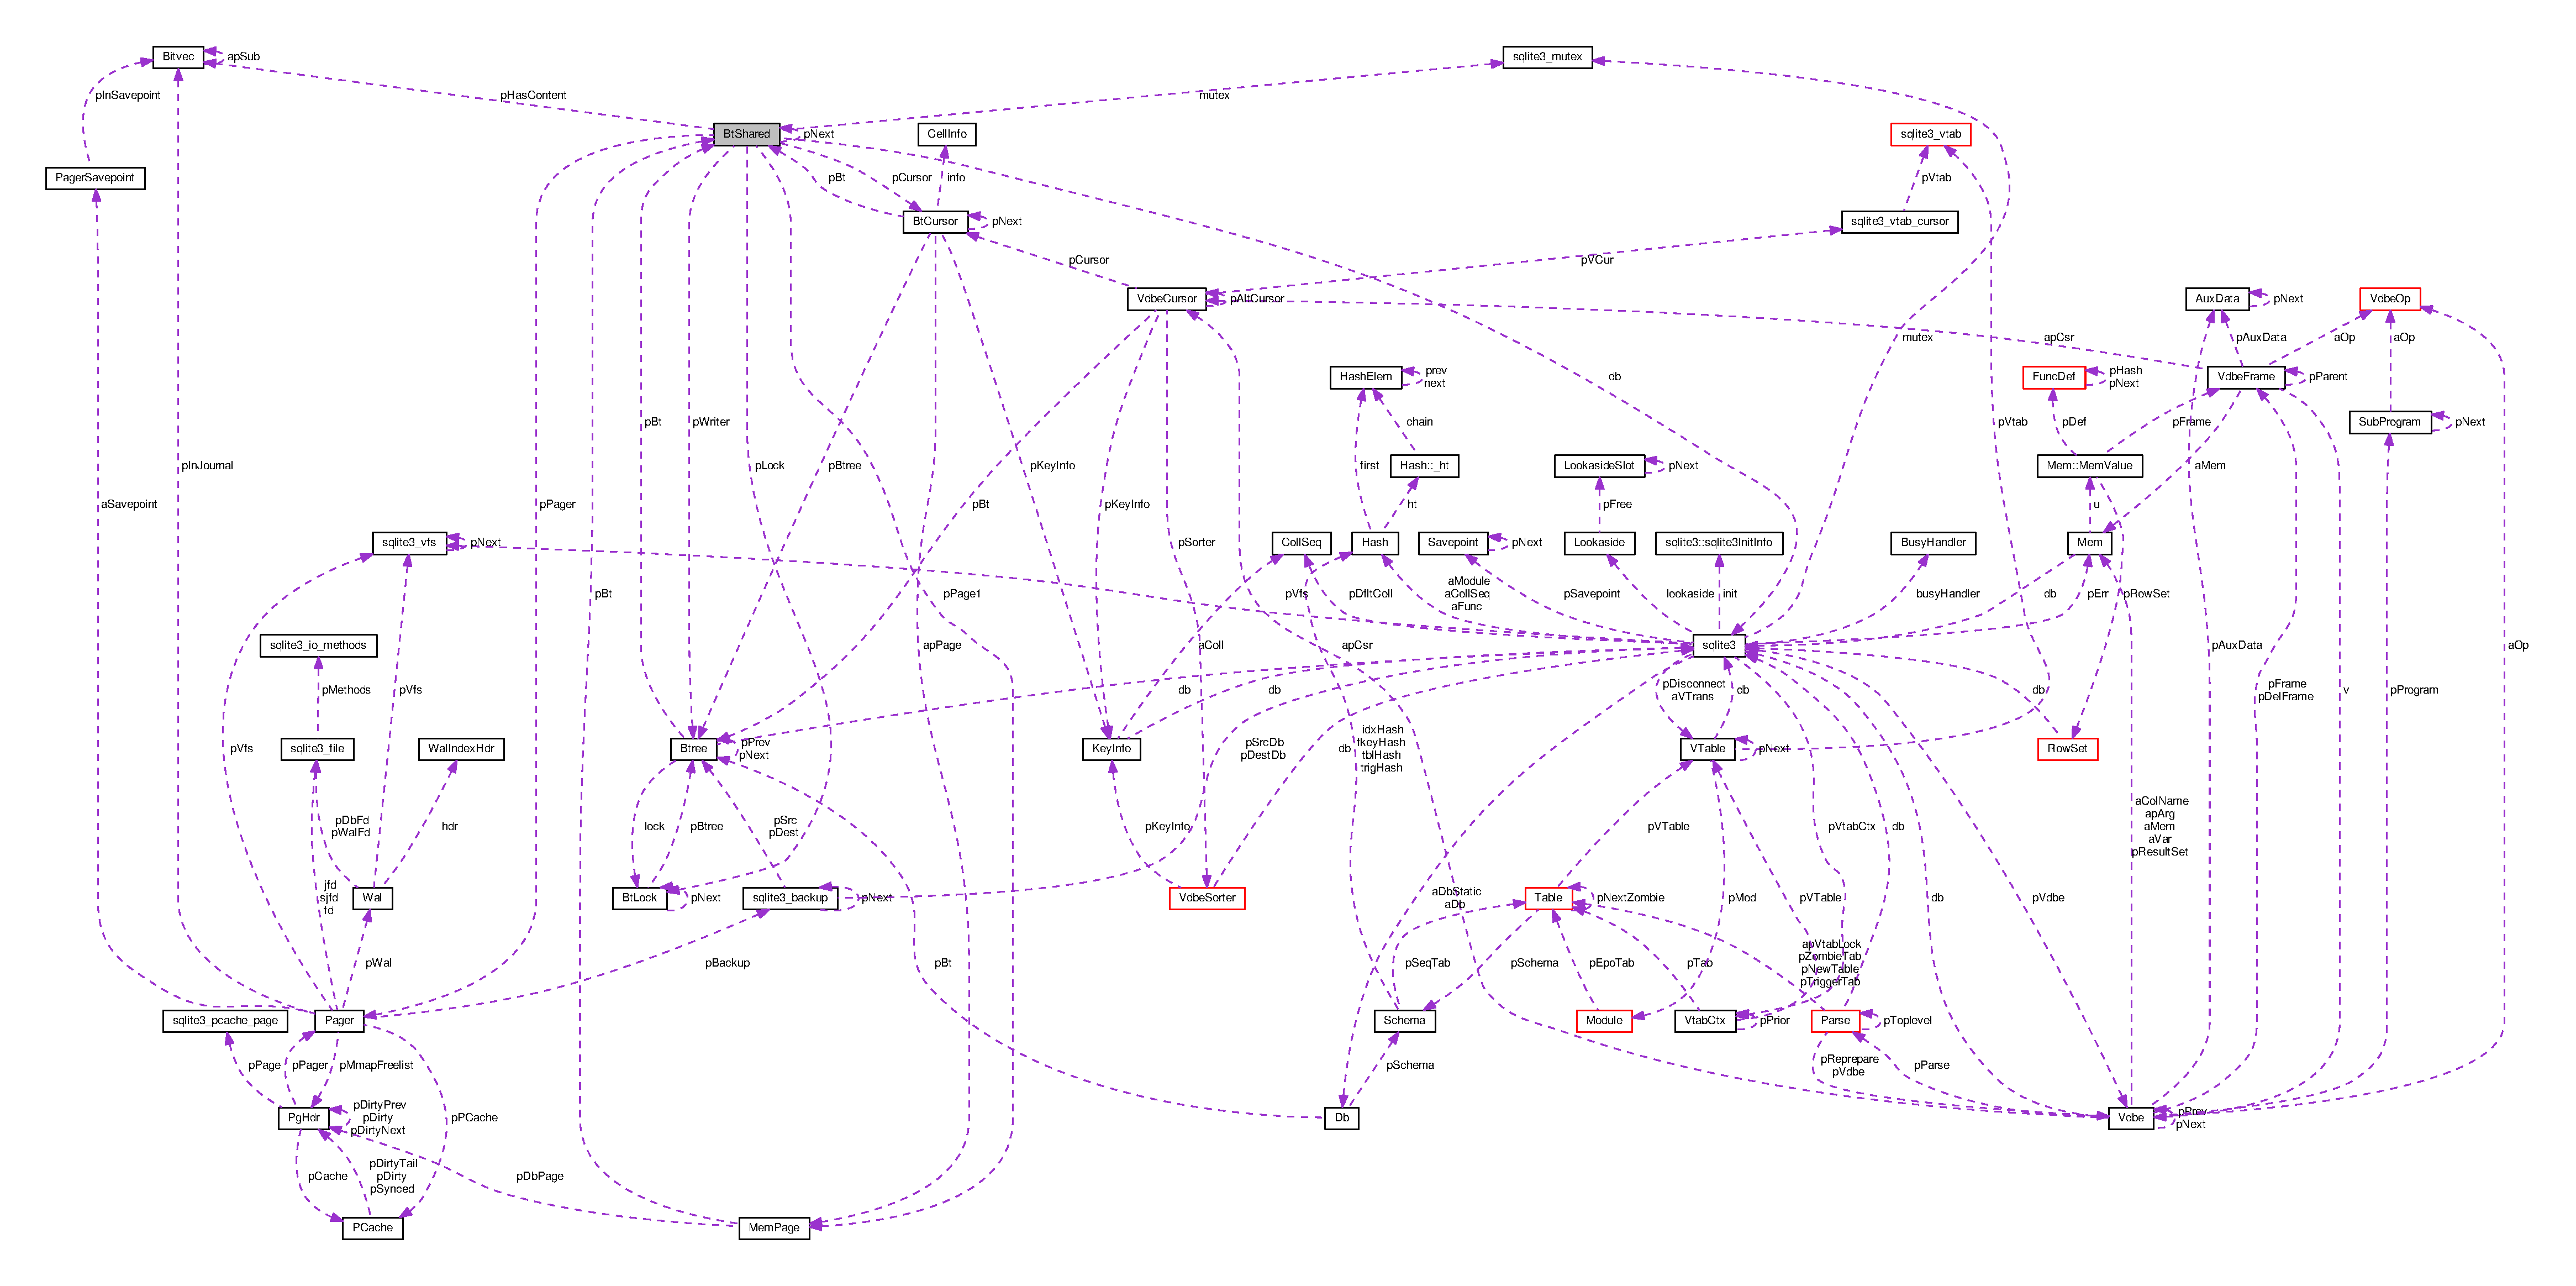
\includegraphics[width=350pt]{structBtShared__coll__graph}
\end{center}
\end{figure}
\subsection*{Public Attributes}
\begin{DoxyCompactItemize}
\item 
\hyperlink{structPager}{Pager} $\ast$ {\bfseries p\+Pager}\hypertarget{structBtShared_ab79703fc47a16446274457588d7eb989}{}\label{structBtShared_ab79703fc47a16446274457588d7eb989}

\item 
\hyperlink{structsqlite3}{sqlite3} $\ast$ {\bfseries db}\hypertarget{structBtShared_a93dafa672793f6117a336d5987951c8e}{}\label{structBtShared_a93dafa672793f6117a336d5987951c8e}

\item 
\hyperlink{structBtCursor}{Bt\+Cursor} $\ast$ {\bfseries p\+Cursor}\hypertarget{structBtShared_a8f8b52dee390e5606e8e2a8511530de7}{}\label{structBtShared_a8f8b52dee390e5606e8e2a8511530de7}

\item 
\hyperlink{structMemPage}{Mem\+Page} $\ast$ {\bfseries p\+Page1}\hypertarget{structBtShared_a296dffd1c698ec175fee109718f32d5d}{}\label{structBtShared_a296dffd1c698ec175fee109718f32d5d}

\item 
u8 {\bfseries open\+Flags}\hypertarget{structBtShared_a8fbc250e23d7c417ccfec8cceb08329d}{}\label{structBtShared_a8fbc250e23d7c417ccfec8cceb08329d}

\item 
u8 {\bfseries auto\+Vacuum}\hypertarget{structBtShared_a770c4f6244d4350f27029cb909902a61}{}\label{structBtShared_a770c4f6244d4350f27029cb909902a61}

\item 
u8 {\bfseries incr\+Vacuum}\hypertarget{structBtShared_a8d8ba06335a63d8a36294a0f1ae8377a}{}\label{structBtShared_a8d8ba06335a63d8a36294a0f1ae8377a}

\item 
u8 {\bfseries b\+Do\+Truncate}\hypertarget{structBtShared_a57de6e40475fc532a5de79760521e957}{}\label{structBtShared_a57de6e40475fc532a5de79760521e957}

\item 
u8 {\bfseries in\+Transaction}\hypertarget{structBtShared_aeaa6c0f33b83434ecee4bd8c4c8df48e}{}\label{structBtShared_aeaa6c0f33b83434ecee4bd8c4c8df48e}

\item 
u8 {\bfseries max1byte\+Payload}\hypertarget{structBtShared_ae0a261001a5237cd705fa16f0d00ad16}{}\label{structBtShared_ae0a261001a5237cd705fa16f0d00ad16}

\item 
u16 {\bfseries bts\+Flags}\hypertarget{structBtShared_a287b7749063c63e45518f72d6f9b3c1d}{}\label{structBtShared_a287b7749063c63e45518f72d6f9b3c1d}

\item 
u16 {\bfseries max\+Local}\hypertarget{structBtShared_a2937d14071841fe0ecae3ce1eb1da96c}{}\label{structBtShared_a2937d14071841fe0ecae3ce1eb1da96c}

\item 
u16 {\bfseries min\+Local}\hypertarget{structBtShared_affb40500b5c63601ef3ca3600983b12c}{}\label{structBtShared_affb40500b5c63601ef3ca3600983b12c}

\item 
u16 {\bfseries max\+Leaf}\hypertarget{structBtShared_a474248f018d24457ec306a7b570d24ce}{}\label{structBtShared_a474248f018d24457ec306a7b570d24ce}

\item 
u16 {\bfseries min\+Leaf}\hypertarget{structBtShared_ad57c14f1681d0e86f1c9a9488013eba0}{}\label{structBtShared_ad57c14f1681d0e86f1c9a9488013eba0}

\item 
u32 {\bfseries page\+Size}\hypertarget{structBtShared_a9e42a71e5e3f98ec1e5b30998b27aae0}{}\label{structBtShared_a9e42a71e5e3f98ec1e5b30998b27aae0}

\item 
u32 {\bfseries usable\+Size}\hypertarget{structBtShared_a3209efe543084a7e60f22913a794f5cb}{}\label{structBtShared_a3209efe543084a7e60f22913a794f5cb}

\item 
int {\bfseries n\+Transaction}\hypertarget{structBtShared_a6101a0e79a95e884ac4dc9c70a947715}{}\label{structBtShared_a6101a0e79a95e884ac4dc9c70a947715}

\item 
u32 {\bfseries n\+Page}\hypertarget{structBtShared_a8679241243f9043ede97b5c57d20c3ea}{}\label{structBtShared_a8679241243f9043ede97b5c57d20c3ea}

\item 
void $\ast$ {\bfseries p\+Schema}\hypertarget{structBtShared_aea3ccb6775c768fbd4f3e29df8cb925d}{}\label{structBtShared_aea3ccb6775c768fbd4f3e29df8cb925d}

\item 
void($\ast$ {\bfseries x\+Free\+Schema} )(void $\ast$)\hypertarget{structBtShared_af8f5f15b6ff3f66a8abb34ddc14d4d7a}{}\label{structBtShared_af8f5f15b6ff3f66a8abb34ddc14d4d7a}

\item 
\hyperlink{structsqlite3__mutex}{sqlite3\+\_\+mutex} $\ast$ {\bfseries mutex}\hypertarget{structBtShared_a454c31d726220bbed43c165e370460c8}{}\label{structBtShared_a454c31d726220bbed43c165e370460c8}

\item 
\hyperlink{structBitvec}{Bitvec} $\ast$ {\bfseries p\+Has\+Content}\hypertarget{structBtShared_ace6191dc3f48f9575d7946ab8cf5b919}{}\label{structBtShared_ace6191dc3f48f9575d7946ab8cf5b919}

\item 
int {\bfseries n\+Ref}\hypertarget{structBtShared_a43d0226fa08d7fae5f992f3a2d72cc08}{}\label{structBtShared_a43d0226fa08d7fae5f992f3a2d72cc08}

\item 
\hyperlink{structBtShared}{Bt\+Shared} $\ast$ {\bfseries p\+Next}\hypertarget{structBtShared_aaa9dd5c5d4ec2bb79ebe4b37ee926ae3}{}\label{structBtShared_aaa9dd5c5d4ec2bb79ebe4b37ee926ae3}

\item 
\hyperlink{structBtLock}{Bt\+Lock} $\ast$ {\bfseries p\+Lock}\hypertarget{structBtShared_af58c79eec88f99ed5a07d8cabf8a1d1a}{}\label{structBtShared_af58c79eec88f99ed5a07d8cabf8a1d1a}

\item 
\hyperlink{structBtree}{Btree} $\ast$ {\bfseries p\+Writer}\hypertarget{structBtShared_ad8b2679e54027d58a3be3afcca4df1d6}{}\label{structBtShared_ad8b2679e54027d58a3be3afcca4df1d6}

\item 
u8 $\ast$ {\bfseries p\+Tmp\+Space}\hypertarget{structBtShared_a89102c20327da8a304f7e95af557bdf4}{}\label{structBtShared_a89102c20327da8a304f7e95af557bdf4}

\end{DoxyCompactItemize}


The documentation for this struct was generated from the following file\+:\begin{DoxyCompactItemize}
\item 
sqlite3.\+c\end{DoxyCompactItemize}

\hypertarget{structBusyHandler}{}\section{Busy\+Handler Struct Reference}
\label{structBusyHandler}\index{Busy\+Handler@{Busy\+Handler}}
\subsection*{Public Attributes}
\begin{DoxyCompactItemize}
\item 
int($\ast$ {\bfseries x\+Func} )(void $\ast$, int)\hypertarget{structBusyHandler_a284037f3ffbbc94d95ec61c39ba8e468}{}\label{structBusyHandler_a284037f3ffbbc94d95ec61c39ba8e468}

\item 
void $\ast$ {\bfseries p\+Arg}\hypertarget{structBusyHandler_a1c793d2b815e79cf3684de46847551bd}{}\label{structBusyHandler_a1c793d2b815e79cf3684de46847551bd}

\item 
int {\bfseries n\+Busy}\hypertarget{structBusyHandler_aac4531c677ed5ae9e4757ca1b02c568b}{}\label{structBusyHandler_aac4531c677ed5ae9e4757ca1b02c568b}

\end{DoxyCompactItemize}


The documentation for this struct was generated from the following file\+:\begin{DoxyCompactItemize}
\item 
sqlite3.\+c\end{DoxyCompactItemize}

\hypertarget{structCellArray}{}\section{Cell\+Array Struct Reference}
\label{structCellArray}\index{Cell\+Array@{Cell\+Array}}


Collaboration diagram for Cell\+Array\+:\nopagebreak
\begin{figure}[H]
\begin{center}
\leavevmode
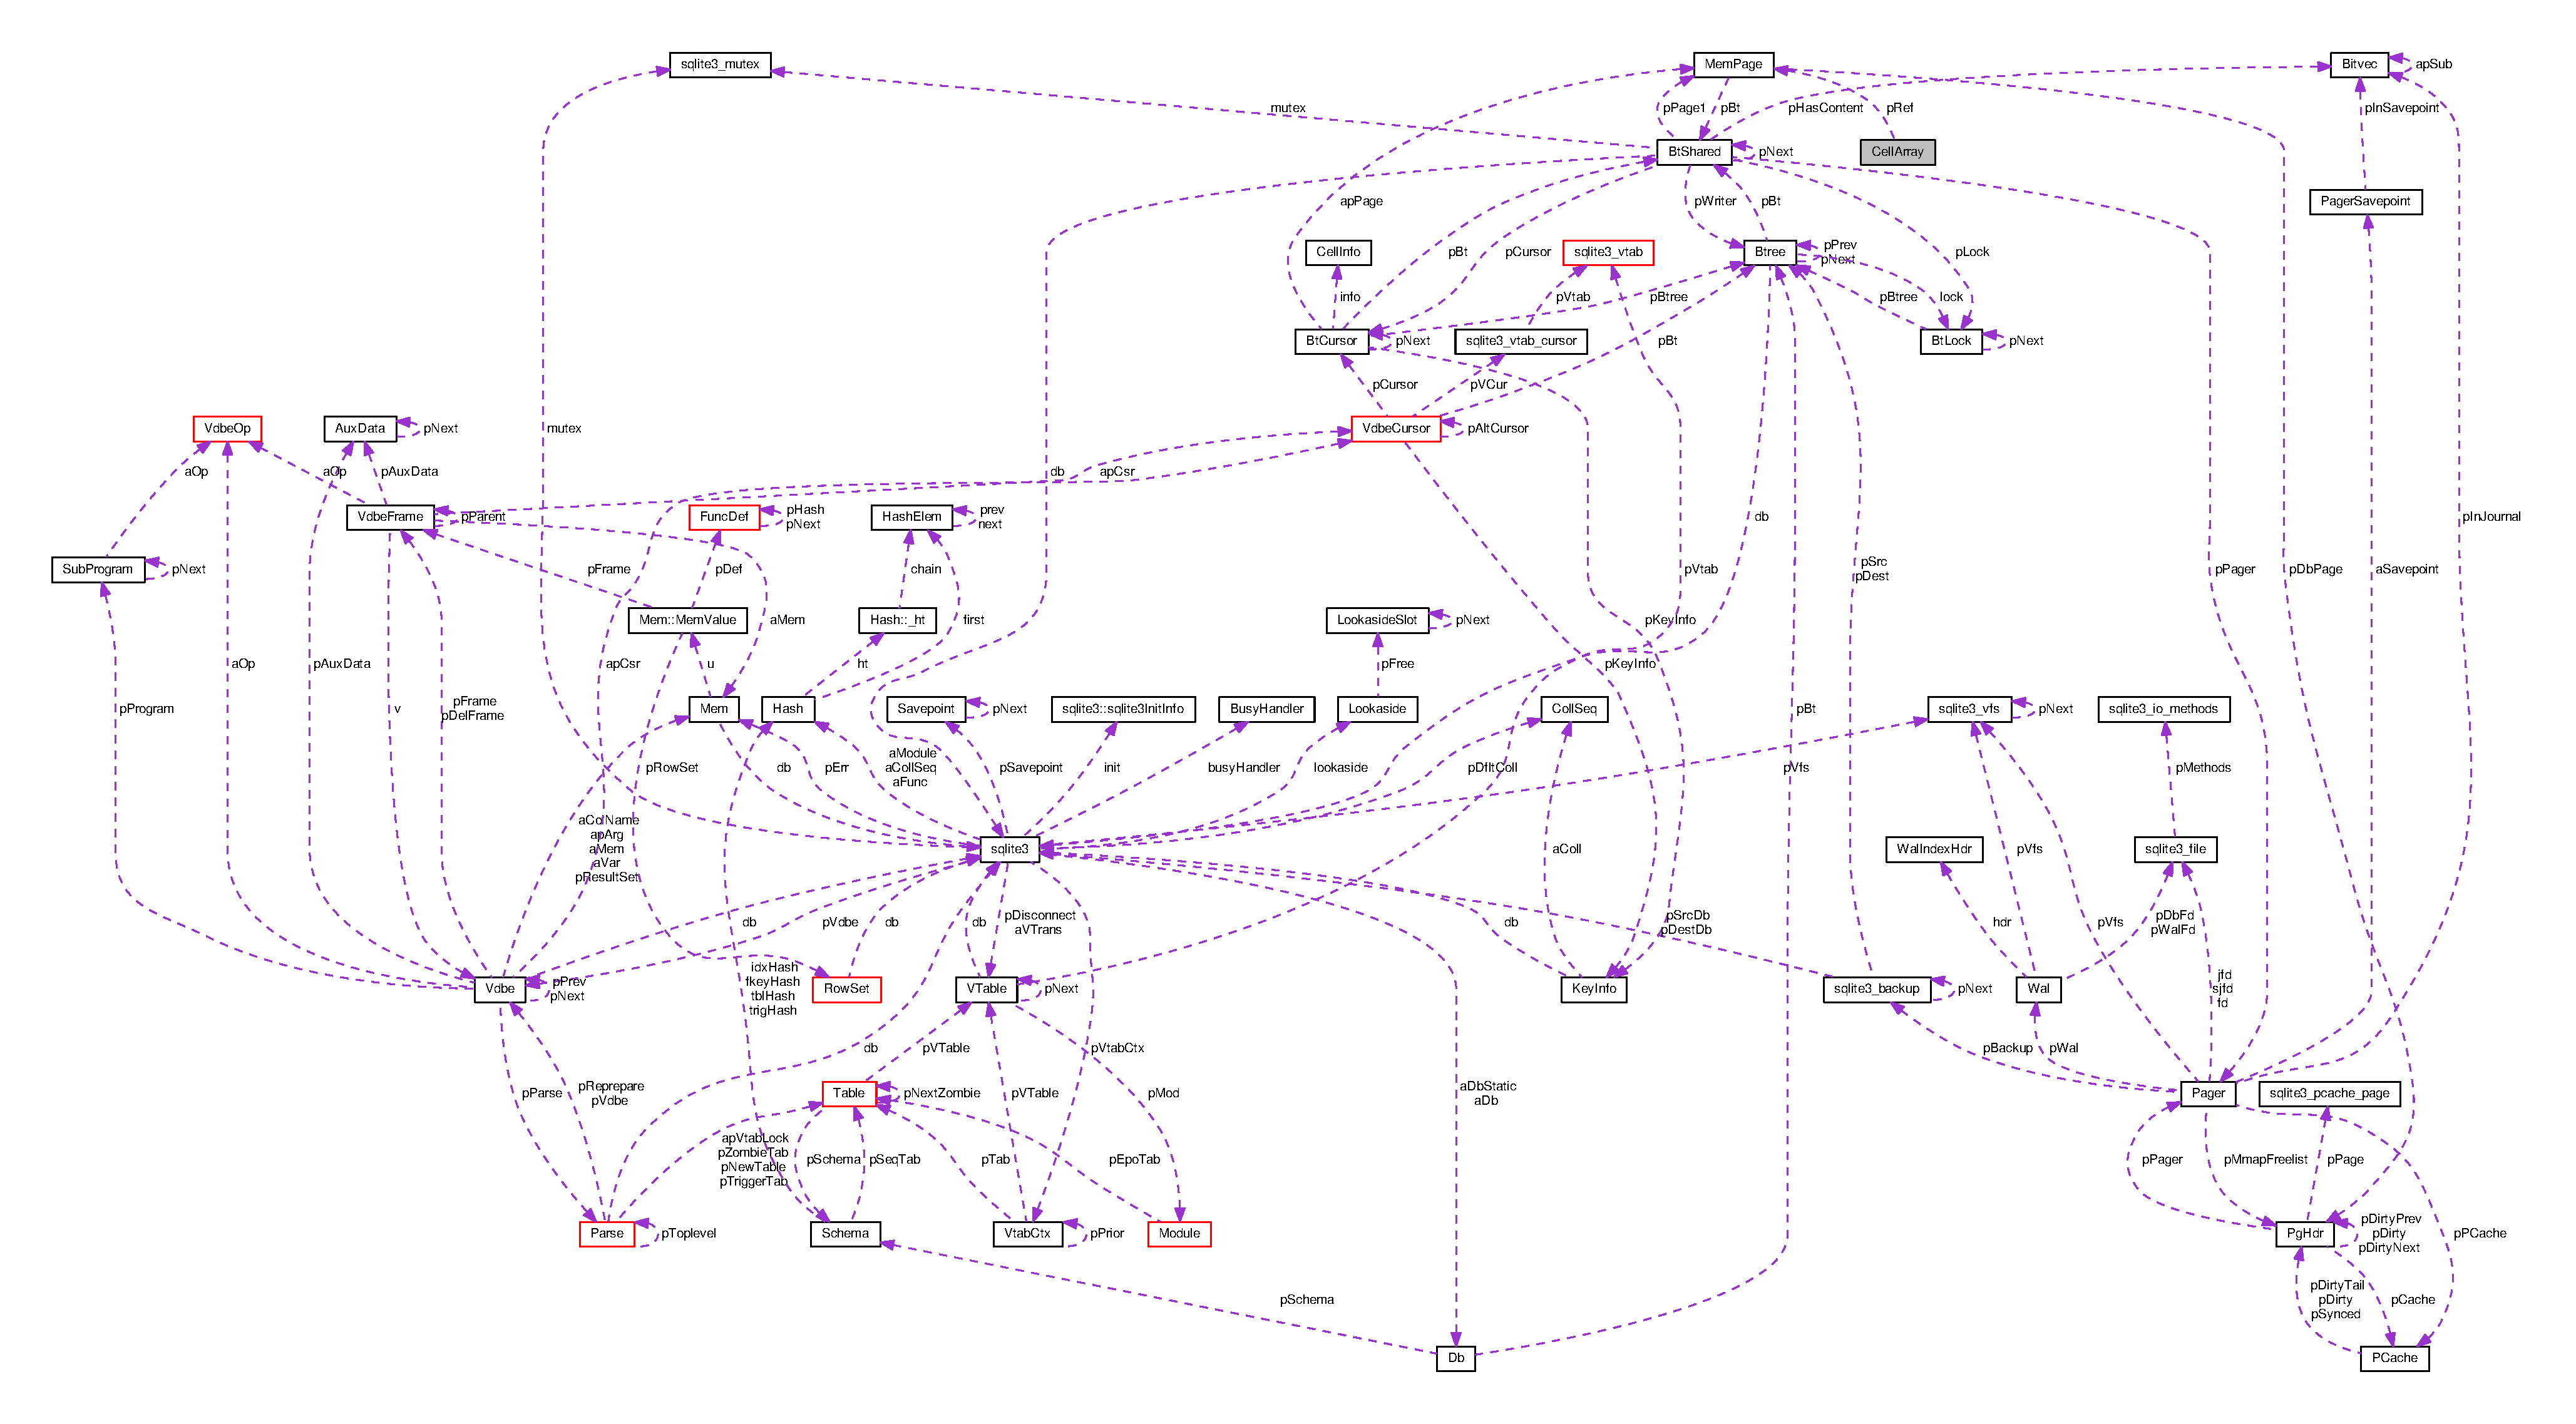
\includegraphics[width=350pt]{structCellArray__coll__graph}
\end{center}
\end{figure}
\subsection*{Public Attributes}
\begin{DoxyCompactItemize}
\item 
int {\bfseries n\+Cell}\hypertarget{structCellArray_a8fe33d4e52945d03ca96b4593995813d}{}\label{structCellArray_a8fe33d4e52945d03ca96b4593995813d}

\item 
\hyperlink{structMemPage}{Mem\+Page} $\ast$ {\bfseries p\+Ref}\hypertarget{structCellArray_a14046c4bbf3090696f4e6909e94fa44d}{}\label{structCellArray_a14046c4bbf3090696f4e6909e94fa44d}

\item 
u8 $\ast$$\ast$ {\bfseries ap\+Cell}\hypertarget{structCellArray_a70f7b19795ffe0c921484857721135a2}{}\label{structCellArray_a70f7b19795ffe0c921484857721135a2}

\item 
u16 $\ast$ {\bfseries sz\+Cell}\hypertarget{structCellArray_a66bb706ff8b01135461c0a9f0b72c47b}{}\label{structCellArray_a66bb706ff8b01135461c0a9f0b72c47b}

\end{DoxyCompactItemize}


The documentation for this struct was generated from the following file\+:\begin{DoxyCompactItemize}
\item 
sqlite3.\+c\end{DoxyCompactItemize}

\hypertarget{structCellInfo}{}\section{Cell\+Info Struct Reference}
\label{structCellInfo}\index{Cell\+Info@{Cell\+Info}}
\subsection*{Public Attributes}
\begin{DoxyCompactItemize}
\item 
i64 {\bfseries n\+Key}\hypertarget{structCellInfo_a542b041b9a54a13f7c6f2fe63e7542c0}{}\label{structCellInfo_a542b041b9a54a13f7c6f2fe63e7542c0}

\item 
u8 $\ast$ {\bfseries p\+Payload}\hypertarget{structCellInfo_abbcd805bfcc10bed2ff5b81aae466940}{}\label{structCellInfo_abbcd805bfcc10bed2ff5b81aae466940}

\item 
u32 {\bfseries n\+Payload}\hypertarget{structCellInfo_ac1e3c1b4216a8e778bbac82907bb1485}{}\label{structCellInfo_ac1e3c1b4216a8e778bbac82907bb1485}

\item 
u16 {\bfseries n\+Local}\hypertarget{structCellInfo_a8cedbcc2c94916fe5798b502c614bb08}{}\label{structCellInfo_a8cedbcc2c94916fe5798b502c614bb08}

\item 
u16 {\bfseries n\+Size}\hypertarget{structCellInfo_ace78ab5eb5337b686e31b895feeb0562}{}\label{structCellInfo_ace78ab5eb5337b686e31b895feeb0562}

\end{DoxyCompactItemize}


The documentation for this struct was generated from the following file\+:\begin{DoxyCompactItemize}
\item 
sqlite3.\+c\end{DoxyCompactItemize}

\hypertarget{classClient}{}\section{Client Class Reference}
\label{classClient}\index{Client@{Client}}


\hyperlink{classClient}{Client} class.  




{\ttfamily \#include $<$Client.\+h$>$}

\subsection*{Public Member Functions}
\begin{DoxyCompactItemize}
\item 
\hyperlink{classClient_a2581a22e25217aafda77c410ee67092c}{Client} (const string \&nam, const string \&add, const string \&cit, const string \&st, const string \&z)
\begin{DoxyCompactList}\small\item\em \hyperlink{classClient}{Client} basic constructor. \end{DoxyCompactList}\item 
void \hyperlink{classClient_ab78b7ecbedb2d6fc0e0df3dfa8c973bc}{set\+Name} (const string \&)\hypertarget{classClient_ab78b7ecbedb2d6fc0e0df3dfa8c973bc}{}\label{classClient_ab78b7ecbedb2d6fc0e0df3dfa8c973bc}

\begin{DoxyCompactList}\small\item\em Setter for name. \end{DoxyCompactList}\item 
string \hyperlink{classClient_a28a677584ad4793b50b31c2e75039e2c}{get\+Name} () const \hypertarget{classClient_a28a677584ad4793b50b31c2e75039e2c}{}\label{classClient_a28a677584ad4793b50b31c2e75039e2c}

\begin{DoxyCompactList}\small\item\em Getter for name. \end{DoxyCompactList}\item 
void \hyperlink{classClient_a69b7a62c15ec787ae86bb66ce4ad312a}{set\+Address} (const string \&add, const string \&cit, const string \&st, const string \&z)
\begin{DoxyCompactList}\small\item\em Setter for address. \end{DoxyCompactList}\item 
string \hyperlink{classClient_a291fb22c4fccb2a6b182c355078553ed}{get\+Address} () const 
\begin{DoxyCompactList}\small\item\em Getter for address. \end{DoxyCompactList}\item 
string \hyperlink{classClient_ad92aa60043bd899cdad19b9ca6a77a2e}{get\+City} () const \hypertarget{classClient_ad92aa60043bd899cdad19b9ca6a77a2e}{}\label{classClient_ad92aa60043bd899cdad19b9ca6a77a2e}

\begin{DoxyCompactList}\small\item\em Getter for city. \end{DoxyCompactList}\item 
string \hyperlink{classClient_adf5ae51b9e301019f229b6dd6893f550}{get\+State} () const \hypertarget{classClient_adf5ae51b9e301019f229b6dd6893f550}{}\label{classClient_adf5ae51b9e301019f229b6dd6893f550}

\begin{DoxyCompactList}\small\item\em Getter for state. \end{DoxyCompactList}\item 
string \hyperlink{classClient_a4595dcdc42fc6dfbf7b53a3dd495b4f1}{get\+Zip} () const \hypertarget{classClient_a4595dcdc42fc6dfbf7b53a3dd495b4f1}{}\label{classClient_a4595dcdc42fc6dfbf7b53a3dd495b4f1}

\begin{DoxyCompactList}\small\item\em Getter for zip. \end{DoxyCompactList}\item 
void \hyperlink{classClient_a2127f6355c6d4fe400f3dd314e1fabc8}{send\+Package} (\hyperlink{classPackage}{Package} $\ast$pack)
\begin{DoxyCompactList}\small\item\em Add a sent package. \end{DoxyCompactList}\item 
vector$<$ \hyperlink{classPackage}{Package} $\ast$ $>$ \hyperlink{classClient_aff47cd6d18feba4c43f7ff495d73f495}{get\+Sent\+Packages} () const 
\begin{DoxyCompactList}\small\item\em Get sent packages. \end{DoxyCompactList}\item 
void \hyperlink{classClient_a1726c784a1c19701a13e12333cf906e5}{receive\+Package} (\hyperlink{classPackage}{Package} $\ast$pack)
\begin{DoxyCompactList}\small\item\em Add a received package. \end{DoxyCompactList}\item 
vector$<$ \hyperlink{classPackage}{Package} $\ast$ $>$ \hyperlink{classClient_aae2dee02f0951f418941234103c275ef}{get\+Received\+Packages} () const 
\begin{DoxyCompactList}\small\item\em Get received packages. \end{DoxyCompactList}\item 
string \hyperlink{classClient_a994ff91075daf477725ca055874e3e22}{to\+String} () const 
\begin{DoxyCompactList}\small\item\em To String. \end{DoxyCompactList}\item 
pair$<$ int, int $>$ \hyperlink{classClient_a00ea13c3af8a5eb6d931e73a5a00bdd4}{get\+Coords} ()
\begin{DoxyCompactList}\small\item\em Returns coordinate pair of client. \end{DoxyCompactList}\item 
\hyperlink{classClient}{Client} $\ast$ \hyperlink{classClient_a81f028cdd0ad080e4739d8b9ad4d757c}{get\+Pointer} ()
\begin{DoxyCompactList}\small\item\em Returns a pointer to this client. \end{DoxyCompactList}\item 
unsigned int \hyperlink{classClient_ad03bbecd42ede5870a9f537fb7c01d97}{get\+ID} ()
\begin{DoxyCompactList}\small\item\em returns the ID of this \hyperlink{classClient}{Client} \end{DoxyCompactList}\end{DoxyCompactItemize}
\subsection*{Static Public Member Functions}
\begin{DoxyCompactItemize}
\item 
static int \hyperlink{classClient_af10ea5348920682f6b7eb8ebcb2c325e}{get\+Count} ()
\begin{DoxyCompactList}\small\item\em Returns the count of total number of clients. \end{DoxyCompactList}\end{DoxyCompactItemize}
\subsection*{Private Member Functions}
\begin{DoxyCompactItemize}
\item 
void \hyperlink{classClient_a6953fb1cd2e5a4fa87ee08479072a402}{parse\+Address} ()
\begin{DoxyCompactList}\small\item\em Parses address into coordinates. \end{DoxyCompactList}\end{DoxyCompactItemize}
\subsection*{Private Attributes}
\begin{DoxyCompactItemize}
\item 
string \hyperlink{classClient_a456e36f9972a8bf3ecdb5f0e70b3bd5d}{name} = \char`\"{}T\+E\+ST\char`\"{}\hypertarget{classClient_a456e36f9972a8bf3ecdb5f0e70b3bd5d}{}\label{classClient_a456e36f9972a8bf3ecdb5f0e70b3bd5d}

\begin{DoxyCompactList}\small\item\em \hyperlink{classClient}{Client} name. \end{DoxyCompactList}\item 
string \hyperlink{classClient_a6355d7fc34358ed4ceac7985f7c46e6e}{address} = \char`\"{}\char`\"{}\hypertarget{classClient_a6355d7fc34358ed4ceac7985f7c46e6e}{}\label{classClient_a6355d7fc34358ed4ceac7985f7c46e6e}

\begin{DoxyCompactList}\small\item\em \hyperlink{classClient}{Client} street address. \end{DoxyCompactList}\item 
string \hyperlink{classClient_a583900f81428de47df9296d49022e022}{city} = \char`\"{}\char`\"{}\hypertarget{classClient_a583900f81428de47df9296d49022e022}{}\label{classClient_a583900f81428de47df9296d49022e022}

\begin{DoxyCompactList}\small\item\em \hyperlink{classClient}{Client} city. \end{DoxyCompactList}\item 
string \hyperlink{classClient_a4e50f1a7dc56fc407b43ee88340ba032}{state} = \char`\"{}\char`\"{}\hypertarget{classClient_a4e50f1a7dc56fc407b43ee88340ba032}{}\label{classClient_a4e50f1a7dc56fc407b43ee88340ba032}

\begin{DoxyCompactList}\small\item\em \hyperlink{classClient}{Client} state. \end{DoxyCompactList}\item 
string \hyperlink{classClient_a9ee92d218e3709abbd9448e162ea306f}{zip} = \char`\"{}\char`\"{}\hypertarget{classClient_a9ee92d218e3709abbd9448e162ea306f}{}\label{classClient_a9ee92d218e3709abbd9448e162ea306f}

\begin{DoxyCompactList}\small\item\em \hyperlink{classClient}{Client} zip. Note as string due to possible upgrades to none numeric zips (eg, UK.) \end{DoxyCompactList}\item 
vector$<$ \hyperlink{classPackage}{Package} $\ast$ $>$ \hyperlink{classClient_a2b2adb035b1729e5914a2ff85e672c88}{sent\+Packages}\hypertarget{classClient_a2b2adb035b1729e5914a2ff85e672c88}{}\label{classClient_a2b2adb035b1729e5914a2ff85e672c88}

\begin{DoxyCompactList}\small\item\em Vector of packages sent by this client. \end{DoxyCompactList}\item 
vector$<$ \hyperlink{classPackage}{Package} $\ast$ $>$ \hyperlink{classClient_ae0b61b806652c0dd46a5ef3e0308fb51}{received\+Packages}\hypertarget{classClient_ae0b61b806652c0dd46a5ef3e0308fb51}{}\label{classClient_ae0b61b806652c0dd46a5ef3e0308fb51}

\begin{DoxyCompactList}\small\item\em Vector of packages received by this client. \end{DoxyCompactList}\item 
pair$<$ int, int $>$ \hyperlink{classClient_a521946a39509ca76f9ef7bea68e47153}{coordinates}\hypertarget{classClient_a521946a39509ca76f9ef7bea68e47153}{}\label{classClient_a521946a39509ca76f9ef7bea68e47153}

\begin{DoxyCompactList}\small\item\em Coordinate pair of address in the city. \end{DoxyCompactList}\item 
const int \hyperlink{classClient_a08c0686b646ab315da55e7f910af7a28}{ID}\hypertarget{classClient_a08c0686b646ab315da55e7f910af7a28}{}\label{classClient_a08c0686b646ab315da55e7f910af7a28}

\begin{DoxyCompactList}\small\item\em ID of client. \end{DoxyCompactList}\end{DoxyCompactItemize}
\subsection*{Static Private Attributes}
\begin{DoxyCompactItemize}
\item 
static int \hyperlink{classClient_a23391f807266e671b35c4a490fca2693}{count} = 0\hypertarget{classClient_a23391f807266e671b35c4a490fca2693}{}\label{classClient_a23391f807266e671b35c4a490fca2693}

\begin{DoxyCompactList}\small\item\em static count of Clients \end{DoxyCompactList}\end{DoxyCompactItemize}
\subsection*{Friends}
\begin{DoxyCompactItemize}
\item 
std\+::ostream \& \hyperlink{classClient_adeb74b47c51aa4da00d60e8ba153a4ed}{operator$<$$<$} (std\+::ostream \&, const \hyperlink{classClient}{Client} \&)\hypertarget{classClient_adeb74b47c51aa4da00d60e8ba153a4ed}{}\label{classClient_adeb74b47c51aa4da00d60e8ba153a4ed}

\begin{DoxyCompactList}\small\item\em Insertion Operator override. \end{DoxyCompactList}\end{DoxyCompactItemize}


\subsection{Detailed Description}
\hyperlink{classClient}{Client} class. 

This client class defines a citizen of the town who can send and receive packages. Each person has a name, address, and vectors representing records of all packages sent and received. 

\subsection{Constructor \& Destructor Documentation}
\index{Client@{Client}!Client@{Client}}
\index{Client@{Client}!Client@{Client}}
\subsubsection[{\texorpdfstring{Client(const string \&nam, const string \&add, const string \&cit, const string \&st, const string \&z)}{Client(const string &nam, const string &add, const string &cit, const string &st, const string &z)}}]{\setlength{\rightskip}{0pt plus 5cm}Client\+::\+Client (
\begin{DoxyParamCaption}
\item[{const string \&}]{nam, }
\item[{const string \&}]{add, }
\item[{const string \&}]{cit, }
\item[{const string \&}]{st, }
\item[{const string \&}]{z}
\end{DoxyParamCaption}
)}\hypertarget{classClient_a2581a22e25217aafda77c410ee67092c}{}\label{classClient_a2581a22e25217aafda77c410ee67092c}


\hyperlink{classClient}{Client} basic constructor. 

Basic constructor. 
\begin{DoxyParams}{Parameters}
{\em nam} & Name of client. \\
\hline
{\em add} & Street address for client. \\
\hline
{\em cit} & City of client \\
\hline
{\em st} & State of client \\
\hline
{\em z} & Z\+IP code of client. Note string usage for international packages. \\
\hline
\end{DoxyParams}


\subsection{Member Function Documentation}
\index{Client@{Client}!get\+Address@{get\+Address}}
\index{get\+Address@{get\+Address}!Client@{Client}}
\subsubsection[{\texorpdfstring{get\+Address() const }{getAddress() const }}]{\setlength{\rightskip}{0pt plus 5cm}string Client\+::get\+Address (
\begin{DoxyParamCaption}
{}
\end{DoxyParamCaption}
) const\hspace{0.3cm}{\ttfamily [inline]}}\hypertarget{classClient_a291fb22c4fccb2a6b182c355078553ed}{}\label{classClient_a291fb22c4fccb2a6b182c355078553ed}


Getter for address. 

\begin{DoxyReturn}{Returns}
String of street address 
\end{DoxyReturn}
\index{Client@{Client}!get\+Coords@{get\+Coords}}
\index{get\+Coords@{get\+Coords}!Client@{Client}}
\subsubsection[{\texorpdfstring{get\+Coords()}{getCoords()}}]{\setlength{\rightskip}{0pt plus 5cm}pair$<$int, int$>$ Client\+::get\+Coords (
\begin{DoxyParamCaption}
{}
\end{DoxyParamCaption}
)\hspace{0.3cm}{\ttfamily [inline]}}\hypertarget{classClient_a00ea13c3af8a5eb6d931e73a5a00bdd4}{}\label{classClient_a00ea13c3af8a5eb6d931e73a5a00bdd4}


Returns coordinate pair of client. 

\begin{DoxyReturn}{Returns}
Coordinate pair of client on City grid. 
\end{DoxyReturn}
\index{Client@{Client}!get\+Count@{get\+Count}}
\index{get\+Count@{get\+Count}!Client@{Client}}
\subsubsection[{\texorpdfstring{get\+Count()}{getCount()}}]{\setlength{\rightskip}{0pt plus 5cm}static int Client\+::get\+Count (
\begin{DoxyParamCaption}
{}
\end{DoxyParamCaption}
)\hspace{0.3cm}{\ttfamily [inline]}, {\ttfamily [static]}}\hypertarget{classClient_af10ea5348920682f6b7eb8ebcb2c325e}{}\label{classClient_af10ea5348920682f6b7eb8ebcb2c325e}


Returns the count of total number of clients. 

\begin{DoxyReturn}{Returns}
int client count 
\end{DoxyReturn}
\index{Client@{Client}!get\+ID@{get\+ID}}
\index{get\+ID@{get\+ID}!Client@{Client}}
\subsubsection[{\texorpdfstring{get\+I\+D()}{getID()}}]{\setlength{\rightskip}{0pt plus 5cm}unsigned int Client\+::get\+ID (
\begin{DoxyParamCaption}
{}
\end{DoxyParamCaption}
)\hspace{0.3cm}{\ttfamily [inline]}}\hypertarget{classClient_ad03bbecd42ede5870a9f537fb7c01d97}{}\label{classClient_ad03bbecd42ede5870a9f537fb7c01d97}


returns the ID of this \hyperlink{classClient}{Client} 

\begin{DoxyReturn}{Returns}
int this client\textquotesingle{}s ID 
\end{DoxyReturn}
\index{Client@{Client}!get\+Pointer@{get\+Pointer}}
\index{get\+Pointer@{get\+Pointer}!Client@{Client}}
\subsubsection[{\texorpdfstring{get\+Pointer()}{getPointer()}}]{\setlength{\rightskip}{0pt plus 5cm}{\bf Client}$\ast$ Client\+::get\+Pointer (
\begin{DoxyParamCaption}
{}
\end{DoxyParamCaption}
)\hspace{0.3cm}{\ttfamily [inline]}}\hypertarget{classClient_a81f028cdd0ad080e4739d8b9ad4d757c}{}\label{classClient_a81f028cdd0ad080e4739d8b9ad4d757c}


Returns a pointer to this client. 

\begin{DoxyReturn}{Returns}
Client$\ast$ pointer to this client 
\end{DoxyReturn}
\index{Client@{Client}!get\+Received\+Packages@{get\+Received\+Packages}}
\index{get\+Received\+Packages@{get\+Received\+Packages}!Client@{Client}}
\subsubsection[{\texorpdfstring{get\+Received\+Packages() const }{getReceivedPackages() const }}]{\setlength{\rightskip}{0pt plus 5cm}vector$<$ {\bf Package} $\ast$ $>$ Client\+::get\+Received\+Packages (
\begin{DoxyParamCaption}
{}
\end{DoxyParamCaption}
) const}\hypertarget{classClient_aae2dee02f0951f418941234103c275ef}{}\label{classClient_aae2dee02f0951f418941234103c275ef}


Get received packages. 

\begin{DoxyReturn}{Returns}
Vector of received packages 
\end{DoxyReturn}
\index{Client@{Client}!get\+Sent\+Packages@{get\+Sent\+Packages}}
\index{get\+Sent\+Packages@{get\+Sent\+Packages}!Client@{Client}}
\subsubsection[{\texorpdfstring{get\+Sent\+Packages() const }{getSentPackages() const }}]{\setlength{\rightskip}{0pt plus 5cm}vector$<$ {\bf Package} $\ast$ $>$ Client\+::get\+Sent\+Packages (
\begin{DoxyParamCaption}
{}
\end{DoxyParamCaption}
) const}\hypertarget{classClient_aff47cd6d18feba4c43f7ff495d73f495}{}\label{classClient_aff47cd6d18feba4c43f7ff495d73f495}


Get sent packages. 

\begin{DoxyReturn}{Returns}
Vector of sent packages 
\end{DoxyReturn}
\index{Client@{Client}!parse\+Address@{parse\+Address}}
\index{parse\+Address@{parse\+Address}!Client@{Client}}
\subsubsection[{\texorpdfstring{parse\+Address()}{parseAddress()}}]{\setlength{\rightskip}{0pt plus 5cm}void Client\+::parse\+Address (
\begin{DoxyParamCaption}
{}
\end{DoxyParamCaption}
)\hspace{0.3cm}{\ttfamily [private]}}\hypertarget{classClient_a6953fb1cd2e5a4fa87ee08479072a402}{}\label{classClient_a6953fb1cd2e5a4fa87ee08479072a402}


Parses address into coordinates. 

Parses the address stored in object variables to Cartesian coordinates. Main Street runs East/\+West at $Y=0$. Central Avenue runs North/\+South at $X=0$. All avenues are N/S, while all streets are E/W. Building numbers are modulus 100, and rounded up or down to the nearest integer. \index{Client@{Client}!receive\+Package@{receive\+Package}}
\index{receive\+Package@{receive\+Package}!Client@{Client}}
\subsubsection[{\texorpdfstring{receive\+Package(\+Package $\ast$pack)}{receivePackage(Package *pack)}}]{\setlength{\rightskip}{0pt plus 5cm}void Client\+::receive\+Package (
\begin{DoxyParamCaption}
\item[{{\bf Package} $\ast$}]{pack}
\end{DoxyParamCaption}
)}\hypertarget{classClient_a1726c784a1c19701a13e12333cf906e5}{}\label{classClient_a1726c784a1c19701a13e12333cf906e5}


Add a received package. 


\begin{DoxyParams}{Parameters}
{\em pack} & pointer to package \\
\hline
\end{DoxyParams}
\index{Client@{Client}!send\+Package@{send\+Package}}
\index{send\+Package@{send\+Package}!Client@{Client}}
\subsubsection[{\texorpdfstring{send\+Package(\+Package $\ast$pack)}{sendPackage(Package *pack)}}]{\setlength{\rightskip}{0pt plus 5cm}void Client\+::send\+Package (
\begin{DoxyParamCaption}
\item[{{\bf Package} $\ast$}]{pack}
\end{DoxyParamCaption}
)}\hypertarget{classClient_a2127f6355c6d4fe400f3dd314e1fabc8}{}\label{classClient_a2127f6355c6d4fe400f3dd314e1fabc8}


Add a sent package. 


\begin{DoxyParams}{Parameters}
{\em pack} & pointer to package \\
\hline
\end{DoxyParams}
\index{Client@{Client}!set\+Address@{set\+Address}}
\index{set\+Address@{set\+Address}!Client@{Client}}
\subsubsection[{\texorpdfstring{set\+Address(const string \&add, const string \&cit, const string \&st, const string \&z)}{setAddress(const string &add, const string &cit, const string &st, const string &z)}}]{\setlength{\rightskip}{0pt plus 5cm}void Client\+::set\+Address (
\begin{DoxyParamCaption}
\item[{const string \&}]{add, }
\item[{const string \&}]{cit, }
\item[{const string \&}]{st, }
\item[{const string \&}]{z}
\end{DoxyParamCaption}
)}\hypertarget{classClient_a69b7a62c15ec787ae86bb66ce4ad312a}{}\label{classClient_a69b7a62c15ec787ae86bb66ce4ad312a}


Setter for address. 

Updates address for client. 
\begin{DoxyParams}{Parameters}
{\em add} & Street address for client. \\
\hline
{\em cit} & City of client \\
\hline
{\em st} & State of client \\
\hline
{\em z} & Z\+IP code of client. Note string usage for international packages. \\
\hline
\end{DoxyParams}
\index{Client@{Client}!to\+String@{to\+String}}
\index{to\+String@{to\+String}!Client@{Client}}
\subsubsection[{\texorpdfstring{to\+String() const }{toString() const }}]{\setlength{\rightskip}{0pt plus 5cm}string Client\+::to\+String (
\begin{DoxyParamCaption}
{}
\end{DoxyParamCaption}
) const}\hypertarget{classClient_a994ff91075daf477725ca055874e3e22}{}\label{classClient_a994ff91075daf477725ca055874e3e22}


To String. 

Converts client information to string for debugging output. \begin{DoxyReturn}{Returns}
String containing client info for std\+::cout
\end{DoxyReturn}
Prints out client\textquotesingle{}s name and address and also all packages associated with the client. Insertion operator only prints name and address. \begin{DoxyReturn}{Returns}
string representation of client and all sent and received packages 
\end{DoxyReturn}


The documentation for this class was generated from the following files\+:\begin{DoxyCompactItemize}
\item 
Client.\+h\item 
Client.\+cpp\end{DoxyCompactItemize}

\hypertarget{structCollSeq}{}\section{Coll\+Seq Struct Reference}
\label{structCollSeq}\index{Coll\+Seq@{Coll\+Seq}}
\subsection*{Public Attributes}
\begin{DoxyCompactItemize}
\item 
char $\ast$ {\bfseries z\+Name}\hypertarget{structCollSeq_a48d6d5f71d4f8a3ab122903464e8b4a1}{}\label{structCollSeq_a48d6d5f71d4f8a3ab122903464e8b4a1}

\item 
u8 {\bfseries enc}\hypertarget{structCollSeq_add27da1a70ed6f538447e9183eeb4838}{}\label{structCollSeq_add27da1a70ed6f538447e9183eeb4838}

\item 
void $\ast$ {\bfseries p\+User}\hypertarget{structCollSeq_a3cee924d41e730ccec7f686eb5b6f041}{}\label{structCollSeq_a3cee924d41e730ccec7f686eb5b6f041}

\item 
int($\ast$ {\bfseries x\+Cmp} )(void $\ast$, int, const void $\ast$, int, const void $\ast$)\hypertarget{structCollSeq_a3f5a0c7eb4da9d8e396138719210f580}{}\label{structCollSeq_a3f5a0c7eb4da9d8e396138719210f580}

\item 
void($\ast$ {\bfseries x\+Del} )(void $\ast$)\hypertarget{structCollSeq_a92c8da8b4021953e5bdc0fd9af077f1f}{}\label{structCollSeq_a92c8da8b4021953e5bdc0fd9af077f1f}

\end{DoxyCompactItemize}


The documentation for this struct was generated from the following file\+:\begin{DoxyCompactItemize}
\item 
sqlite3.\+c\end{DoxyCompactItemize}

\hypertarget{structColumn}{}\section{Column Struct Reference}
\label{structColumn}\index{Column@{Column}}


Collaboration diagram for Column\+:
% FIG 0
\subsection*{Public Attributes}
\begin{DoxyCompactItemize}
\item 
char $\ast$ {\bfseries z\+Name}\hypertarget{structColumn_a6450a4e9fde68b3a2d79425d826eccc3}{}\label{structColumn_a6450a4e9fde68b3a2d79425d826eccc3}

\item 
\hyperlink{structExpr}{Expr} $\ast$ {\bfseries p\+Dflt}\hypertarget{structColumn_ac4178f302df70048235660979f84ffe4}{}\label{structColumn_ac4178f302df70048235660979f84ffe4}

\item 
char $\ast$ {\bfseries z\+Coll}\hypertarget{structColumn_aa95909d5c77b321258622ed28d7b96eb}{}\label{structColumn_aa95909d5c77b321258622ed28d7b96eb}

\item 
u8 {\bfseries not\+Null}\hypertarget{structColumn_a852e9a4c1c327a64d9b051dcafda3841}{}\label{structColumn_a852e9a4c1c327a64d9b051dcafda3841}

\item 
char {\bfseries affinity}\hypertarget{structColumn_ac9d6fe31c45888cecaf3f5ad5b93bf23}{}\label{structColumn_ac9d6fe31c45888cecaf3f5ad5b93bf23}

\item 
u8 {\bfseries sz\+Est}\hypertarget{structColumn_a6d28f0023e550ea38ad2ab544942114d}{}\label{structColumn_a6d28f0023e550ea38ad2ab544942114d}

\item 
u8 {\bfseries col\+Flags}\hypertarget{structColumn_aadfed8f7a238c314e1499a6c4090f920}{}\label{structColumn_aadfed8f7a238c314e1499a6c4090f920}

\end{DoxyCompactItemize}


The documentation for this struct was generated from the following file\+:\begin{DoxyCompactItemize}
\item 
sqlite3.\+c\end{DoxyCompactItemize}

\hypertarget{structcompareInfo}{}\section{compare\+Info Struct Reference}
\label{structcompareInfo}\index{compare\+Info@{compare\+Info}}
\subsection*{Public Attributes}
\begin{DoxyCompactItemize}
\item 
u8 {\bfseries match\+All}\hypertarget{structcompareInfo_a1161e850029ef556e6daee856d32b2e2}{}\label{structcompareInfo_a1161e850029ef556e6daee856d32b2e2}

\item 
u8 {\bfseries match\+One}\hypertarget{structcompareInfo_ab9aabbf6d3df26bad786b532330a2fd7}{}\label{structcompareInfo_ab9aabbf6d3df26bad786b532330a2fd7}

\item 
u8 {\bfseries match\+Set}\hypertarget{structcompareInfo_a5d2ff58a72c9eb7d22f18915c1751655}{}\label{structcompareInfo_a5d2ff58a72c9eb7d22f18915c1751655}

\item 
u8 {\bfseries no\+Case}\hypertarget{structcompareInfo_a6de76861b066547321f7a255cb7042ab}{}\label{structcompareInfo_a6de76861b066547321f7a255cb7042ab}

\end{DoxyCompactItemize}


The documentation for this struct was generated from the following file\+:\begin{DoxyCompactItemize}
\item 
sqlite3.\+c\end{DoxyCompactItemize}

\hypertarget{structCountCtx}{}\section{Count\+Ctx Struct Reference}
\label{structCountCtx}\index{Count\+Ctx@{Count\+Ctx}}
\subsection*{Public Attributes}
\begin{DoxyCompactItemize}
\item 
i64 {\bfseries n}\hypertarget{structCountCtx_a141c718918dbfaa183f772bfd7a516f4}{}\label{structCountCtx_a141c718918dbfaa183f772bfd7a516f4}

\end{DoxyCompactItemize}


The documentation for this struct was generated from the following file\+:\begin{DoxyCompactItemize}
\item 
sqlite3.\+c\end{DoxyCompactItemize}

\hypertarget{structWith_1_1Cte}{}\section{With\+:\+:Cte Struct Reference}
\label{structWith_1_1Cte}\index{With\+::\+Cte@{With\+::\+Cte}}


Collaboration diagram for With\+:\+:Cte\+:\nopagebreak
\begin{figure}[H]
\begin{center}
\leavevmode
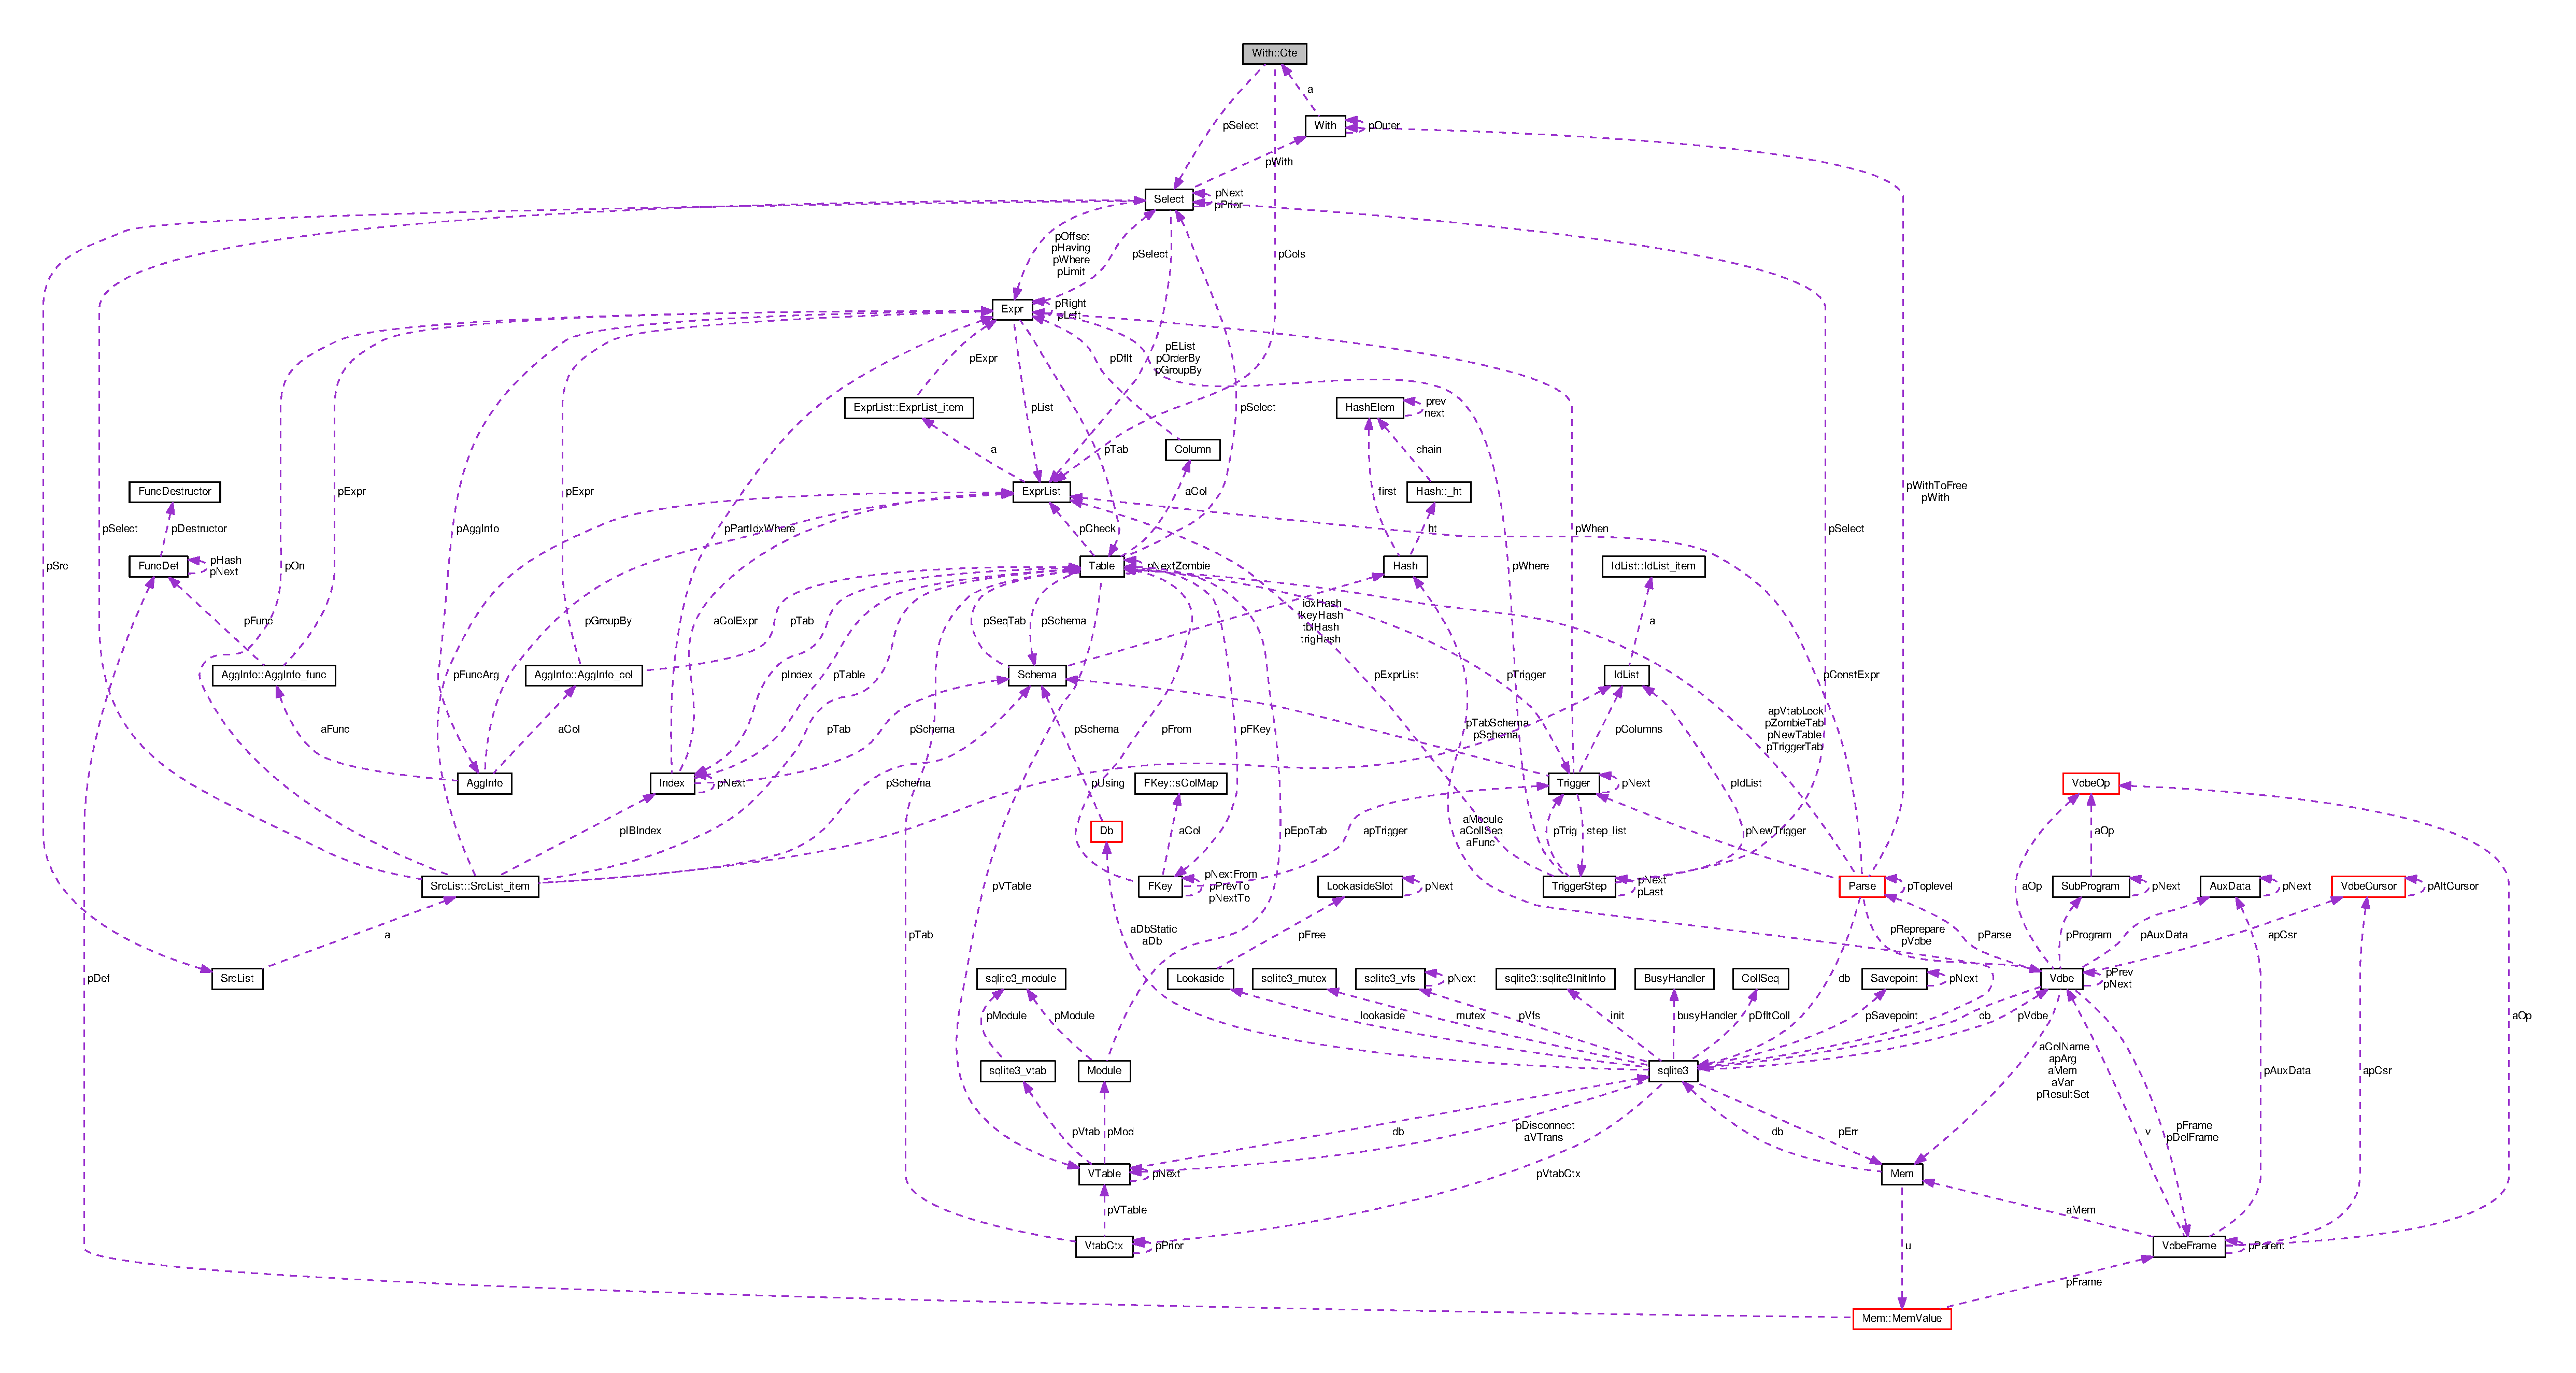
\includegraphics[width=350pt]{structWith_1_1Cte__coll__graph}
\end{center}
\end{figure}
\subsection*{Public Attributes}
\begin{DoxyCompactItemize}
\item 
char $\ast$ {\bfseries z\+Name}\hypertarget{structWith_1_1Cte_a3ce66361944f92f0d3fc354025320dd6}{}\label{structWith_1_1Cte_a3ce66361944f92f0d3fc354025320dd6}

\item 
\hyperlink{structExprList}{Expr\+List} $\ast$ {\bfseries p\+Cols}\hypertarget{structWith_1_1Cte_a9e43b7bf43ff5878c465f683fc464456}{}\label{structWith_1_1Cte_a9e43b7bf43ff5878c465f683fc464456}

\item 
\hyperlink{structSelect}{Select} $\ast$ {\bfseries p\+Select}\hypertarget{structWith_1_1Cte_a90fd9f2a4529a6fd1e75cabeccec16cd}{}\label{structWith_1_1Cte_a90fd9f2a4529a6fd1e75cabeccec16cd}

\item 
const char $\ast$ {\bfseries z\+Cte\+Err}\hypertarget{structWith_1_1Cte_a2e0558ed352afe93f08cb8a9ed407223}{}\label{structWith_1_1Cte_a2e0558ed352afe93f08cb8a9ed407223}

\end{DoxyCompactItemize}


The documentation for this struct was generated from the following file\+:\begin{DoxyCompactItemize}
\item 
sqlite3.\+c\end{DoxyCompactItemize}

\hypertarget{structDateTime}{}\section{Date\+Time Struct Reference}
\label{structDateTime}\index{Date\+Time@{Date\+Time}}
\subsection*{Public Attributes}
\begin{DoxyCompactItemize}
\item 
sqlite3\+\_\+int64 {\bfseries i\+JD}\hypertarget{structDateTime_ae5043d34fa3c3c4dc1121fec886c6f10}{}\label{structDateTime_ae5043d34fa3c3c4dc1121fec886c6f10}

\item 
int {\bfseries Y}\hypertarget{structDateTime_ad39449618b2a15128e32766a208753cf}{}\label{structDateTime_ad39449618b2a15128e32766a208753cf}

\item 
int {\bfseries M}\hypertarget{structDateTime_a00e6515603bb5d7c5ce79d3a5a6438a7}{}\label{structDateTime_a00e6515603bb5d7c5ce79d3a5a6438a7}

\item 
int {\bfseries D}\hypertarget{structDateTime_a979ec52428a05d2f2ed827345a416fa6}{}\label{structDateTime_a979ec52428a05d2f2ed827345a416fa6}

\item 
int {\bfseries h}\hypertarget{structDateTime_a2146547149b65f64e07e1ac6ed8654b6}{}\label{structDateTime_a2146547149b65f64e07e1ac6ed8654b6}

\item 
int {\bfseries m}\hypertarget{structDateTime_ac5db527c48331a515bea3b828d1a2254}{}\label{structDateTime_ac5db527c48331a515bea3b828d1a2254}

\item 
int {\bfseries tz}\hypertarget{structDateTime_a7f5c2e587ee18014982d85eb616f09b8}{}\label{structDateTime_a7f5c2e587ee18014982d85eb616f09b8}

\item 
double {\bfseries s}\hypertarget{structDateTime_a69a803afb69b74206418bda0bc1bcaa2}{}\label{structDateTime_a69a803afb69b74206418bda0bc1bcaa2}

\item 
char {\bfseries valid\+Y\+MD}\hypertarget{structDateTime_aaa042bec0879cd922039062433f4b26f}{}\label{structDateTime_aaa042bec0879cd922039062433f4b26f}

\item 
char {\bfseries valid\+H\+MS}\hypertarget{structDateTime_aba26b32c6142cf6bfc09db3088b90add}{}\label{structDateTime_aba26b32c6142cf6bfc09db3088b90add}

\item 
char {\bfseries valid\+JD}\hypertarget{structDateTime_a1962742892150a03dc5d302f43efbb04}{}\label{structDateTime_a1962742892150a03dc5d302f43efbb04}

\item 
char {\bfseries valid\+TZ}\hypertarget{structDateTime_af3dfda2bdbb2183dc1b94f449701b81e}{}\label{structDateTime_af3dfda2bdbb2183dc1b94f449701b81e}

\item 
char {\bfseries tz\+Set}\hypertarget{structDateTime_a1d3f01eb19ad909d0e2a13c25cf4e48e}{}\label{structDateTime_a1d3f01eb19ad909d0e2a13c25cf4e48e}

\end{DoxyCompactItemize}


The documentation for this struct was generated from the following file\+:\begin{DoxyCompactItemize}
\item 
sqlite3.\+c\end{DoxyCompactItemize}

\hypertarget{structDb}{}\section{Db Struct Reference}
\label{structDb}\index{Db@{Db}}


Collaboration diagram for Db\+:\nopagebreak
\begin{figure}[H]
\begin{center}
\leavevmode
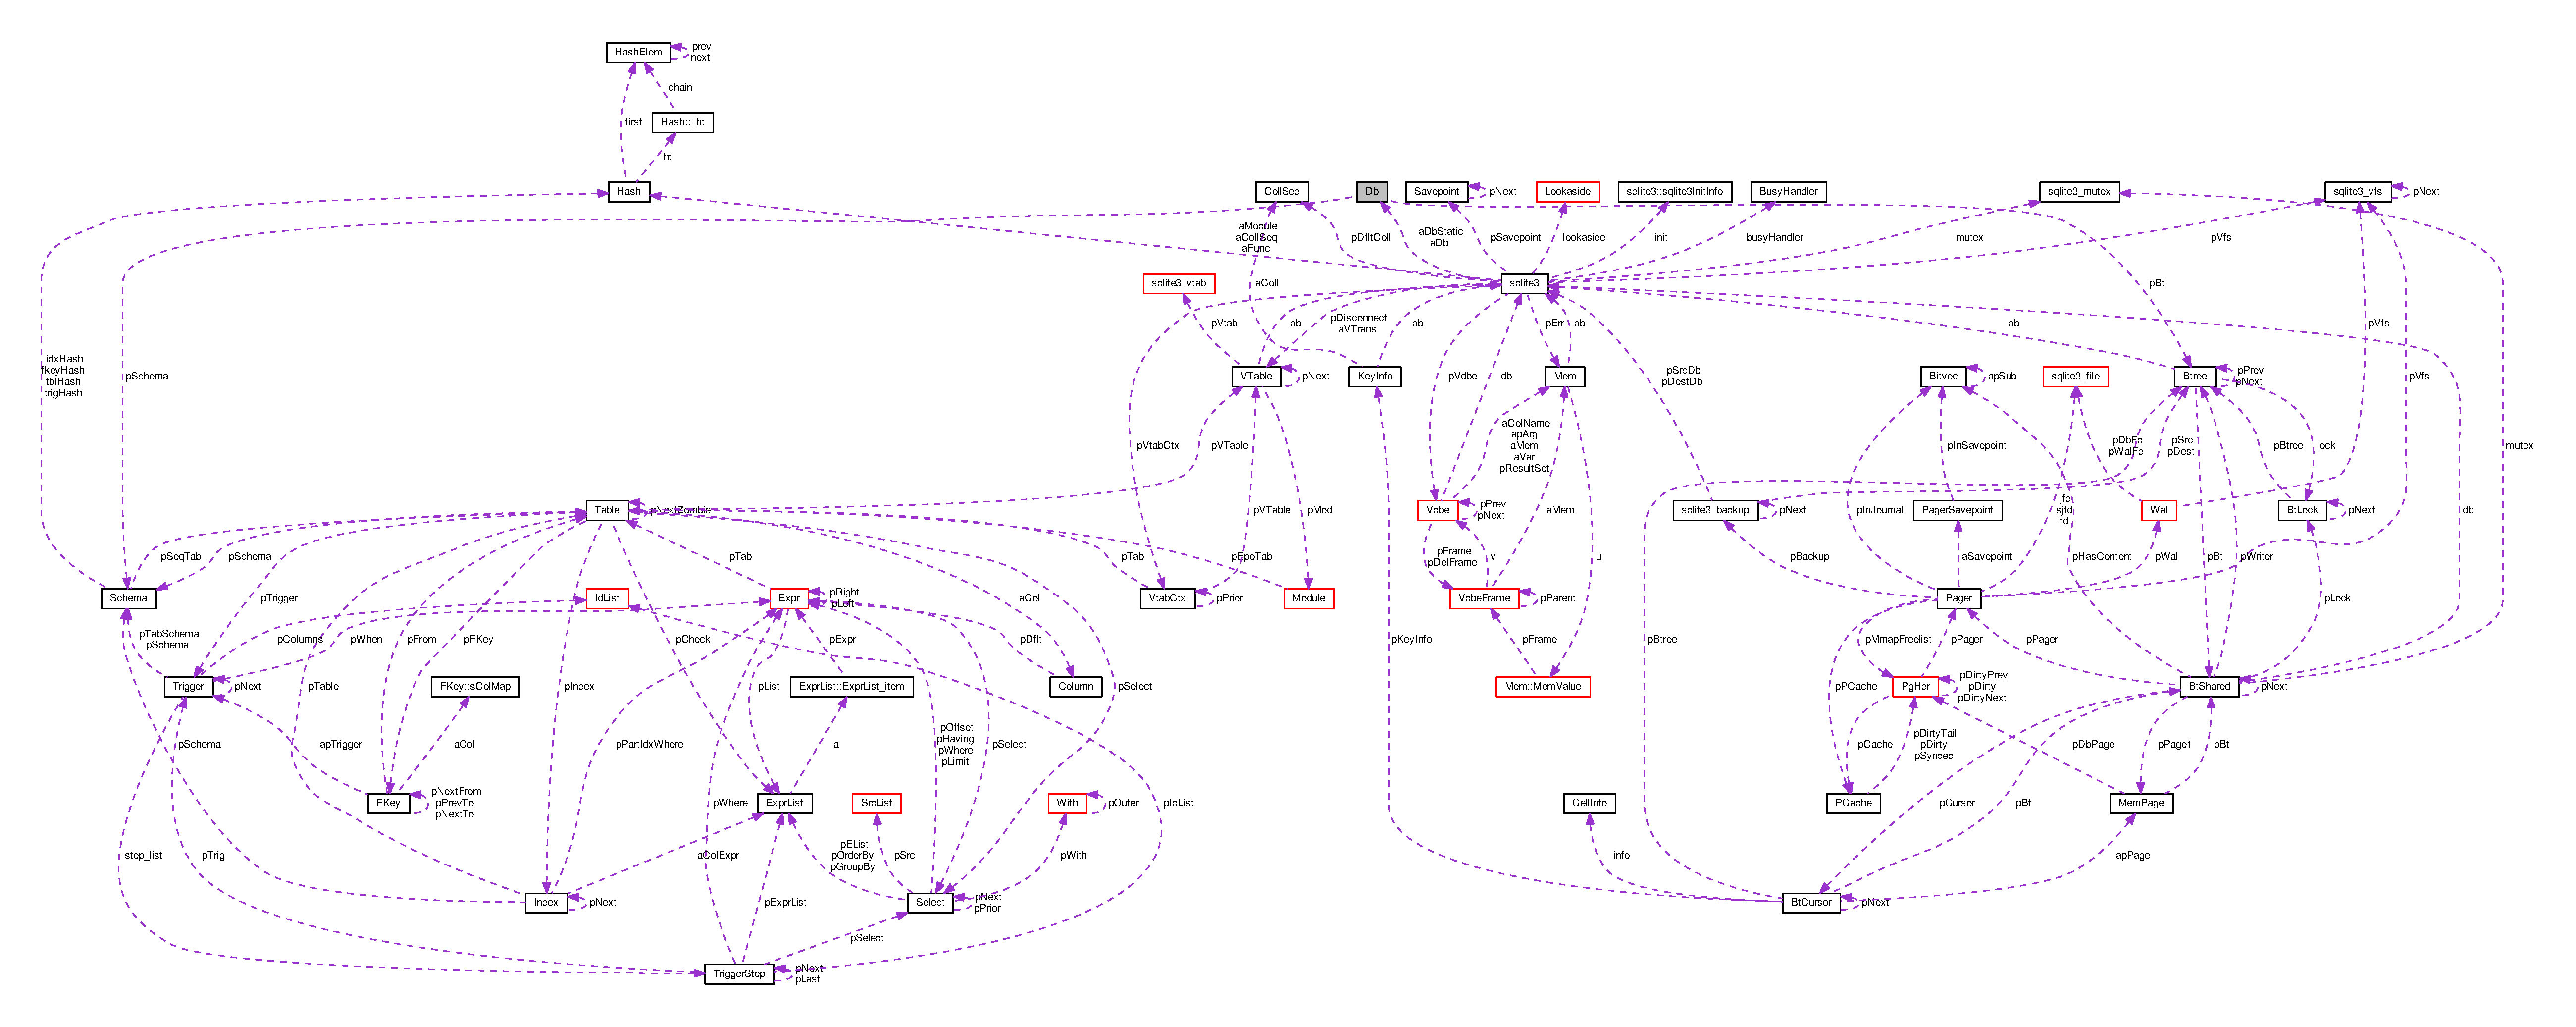
\includegraphics[width=350pt]{structDb__coll__graph}
\end{center}
\end{figure}
\subsection*{Public Attributes}
\begin{DoxyCompactItemize}
\item 
char $\ast$ {\bfseries z\+Db\+S\+Name}\hypertarget{structDb_a3129038e85466e764d1c866af0c9b3a2}{}\label{structDb_a3129038e85466e764d1c866af0c9b3a2}

\item 
\hyperlink{structBtree}{Btree} $\ast$ {\bfseries p\+Bt}\hypertarget{structDb_a0633e5a6abfc39246d07cc6a417a5852}{}\label{structDb_a0633e5a6abfc39246d07cc6a417a5852}

\item 
u8 {\bfseries safety\+\_\+level}\hypertarget{structDb_a04597a5c023d8b328193450b177ff24c}{}\label{structDb_a04597a5c023d8b328193450b177ff24c}

\item 
u8 {\bfseries b\+Sync\+Set}\hypertarget{structDb_a37f3a8593c9d7042c1c26dd492c409e4}{}\label{structDb_a37f3a8593c9d7042c1c26dd492c409e4}

\item 
\hyperlink{structSchema}{Schema} $\ast$ {\bfseries p\+Schema}\hypertarget{structDb_afd8647a83a4a7053231b92814520d6d4}{}\label{structDb_afd8647a83a4a7053231b92814520d6d4}

\end{DoxyCompactItemize}


The documentation for this struct was generated from the following file\+:\begin{DoxyCompactItemize}
\item 
sqlite3.\+c\end{DoxyCompactItemize}

\hypertarget{structDbFixer}{}\section{Db\+Fixer Struct Reference}
\label{structDbFixer}\index{Db\+Fixer@{Db\+Fixer}}


Collaboration diagram for Db\+Fixer\+:\nopagebreak
\begin{figure}[H]
\begin{center}
\leavevmode
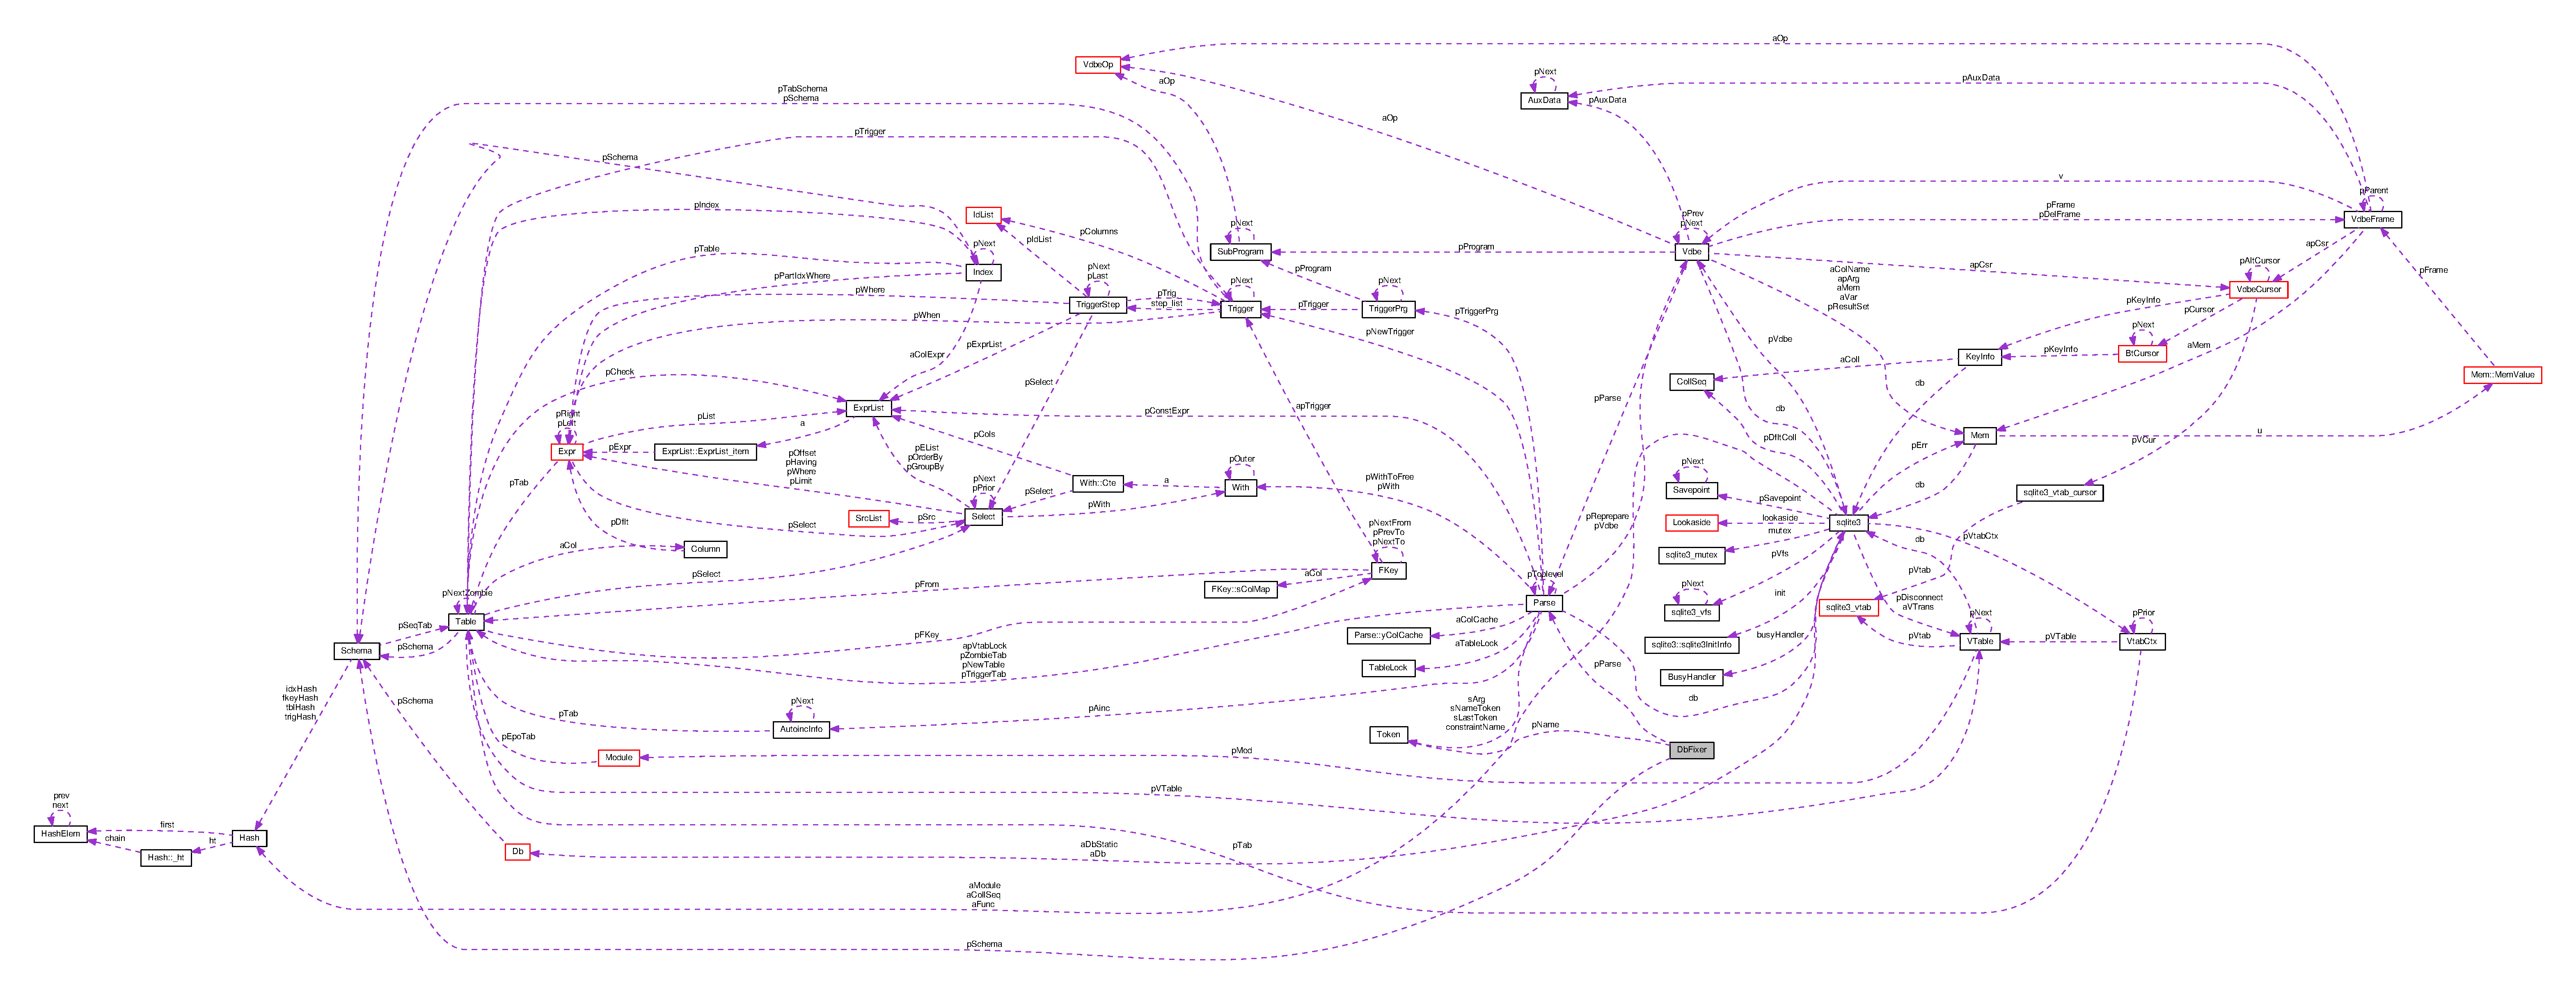
\includegraphics[width=350pt]{structDbFixer__coll__graph}
\end{center}
\end{figure}
\subsection*{Public Attributes}
\begin{DoxyCompactItemize}
\item 
\hyperlink{structParse}{Parse} $\ast$ {\bfseries p\+Parse}\hypertarget{structDbFixer_ac5c9b8bca3b05a66faea11dd998bf6f6}{}\label{structDbFixer_ac5c9b8bca3b05a66faea11dd998bf6f6}

\item 
\hyperlink{structSchema}{Schema} $\ast$ {\bfseries p\+Schema}\hypertarget{structDbFixer_a302dd5335c8a982deda5bf04bae00363}{}\label{structDbFixer_a302dd5335c8a982deda5bf04bae00363}

\item 
int {\bfseries b\+Var\+Only}\hypertarget{structDbFixer_aebd8549176b84c8c71069ed4d77ad6af}{}\label{structDbFixer_aebd8549176b84c8c71069ed4d77ad6af}

\item 
const char $\ast$ {\bfseries z\+Db}\hypertarget{structDbFixer_aba91df5965a99915d9180805d02c4a7f}{}\label{structDbFixer_aba91df5965a99915d9180805d02c4a7f}

\item 
const char $\ast$ {\bfseries z\+Type}\hypertarget{structDbFixer_ae4748d9e97560b7b332527434408c2e8}{}\label{structDbFixer_ae4748d9e97560b7b332527434408c2e8}

\item 
const \hyperlink{structToken}{Token} $\ast$ {\bfseries p\+Name}\hypertarget{structDbFixer_aedee20e10de7337651b84656ee81b39c}{}\label{structDbFixer_aedee20e10de7337651b84656ee81b39c}

\end{DoxyCompactItemize}


The documentation for this struct was generated from the following file\+:\begin{DoxyCompactItemize}
\item 
sqlite3.\+c\end{DoxyCompactItemize}

\hypertarget{structDistinctCtx}{}\section{Distinct\+Ctx Struct Reference}
\label{structDistinctCtx}\index{Distinct\+Ctx@{Distinct\+Ctx}}
\subsection*{Public Attributes}
\begin{DoxyCompactItemize}
\item 
u8 {\bfseries is\+Tnct}\hypertarget{structDistinctCtx_aaaa3b23ad86358ba11b4da77cd753bbd}{}\label{structDistinctCtx_aaaa3b23ad86358ba11b4da77cd753bbd}

\item 
u8 {\bfseries e\+Tnct\+Type}\hypertarget{structDistinctCtx_ae57f819b64420f943f21d8d0e9c36205}{}\label{structDistinctCtx_ae57f819b64420f943f21d8d0e9c36205}

\item 
int {\bfseries tab\+Tnct}\hypertarget{structDistinctCtx_af4514e425f99659e97b2bbe756716517}{}\label{structDistinctCtx_af4514e425f99659e97b2bbe756716517}

\item 
int {\bfseries addr\+Tnct}\hypertarget{structDistinctCtx_a897fdd9a1025f3d6c438a5113cf925d2}{}\label{structDistinctCtx_a897fdd9a1025f3d6c438a5113cf925d2}

\end{DoxyCompactItemize}


The documentation for this struct was generated from the following file\+:\begin{DoxyCompactItemize}
\item 
sqlite3.\+c\end{DoxyCompactItemize}

\hypertarget{structet__info}{}\section{et\+\_\+info Struct Reference}
\label{structet__info}\index{et\+\_\+info@{et\+\_\+info}}
\subsection*{Public Attributes}
\begin{DoxyCompactItemize}
\item 
char {\bfseries fmttype}\hypertarget{structet__info_a1740af27f0c9d5840e7dda59a129aa4b}{}\label{structet__info_a1740af27f0c9d5840e7dda59a129aa4b}

\item 
et\+Byte {\bfseries base}\hypertarget{structet__info_a20f5a4c11c7aa1d9c777805d11965c66}{}\label{structet__info_a20f5a4c11c7aa1d9c777805d11965c66}

\item 
et\+Byte {\bfseries flags}\hypertarget{structet__info_a8f11646aaec803f0870683dc3ba2f756}{}\label{structet__info_a8f11646aaec803f0870683dc3ba2f756}

\item 
et\+Byte {\bfseries type}\hypertarget{structet__info_a148bd1efa49018c9a723701ba5747825}{}\label{structet__info_a148bd1efa49018c9a723701ba5747825}

\item 
et\+Byte {\bfseries charset}\hypertarget{structet__info_a77131acb7479b0e6aad61af0901e11c2}{}\label{structet__info_a77131acb7479b0e6aad61af0901e11c2}

\item 
et\+Byte {\bfseries prefix}\hypertarget{structet__info_a23cc866bf202c34e49bd49599b051628}{}\label{structet__info_a23cc866bf202c34e49bd49599b051628}

\end{DoxyCompactItemize}


The documentation for this struct was generated from the following file\+:\begin{DoxyCompactItemize}
\item 
sqlite3.\+c\end{DoxyCompactItemize}

\hypertarget{structExpr}{}\section{Expr Struct Reference}
\label{structExpr}\index{Expr@{Expr}}


Collaboration diagram for Expr\+:\nopagebreak
\begin{figure}[H]
\begin{center}
\leavevmode
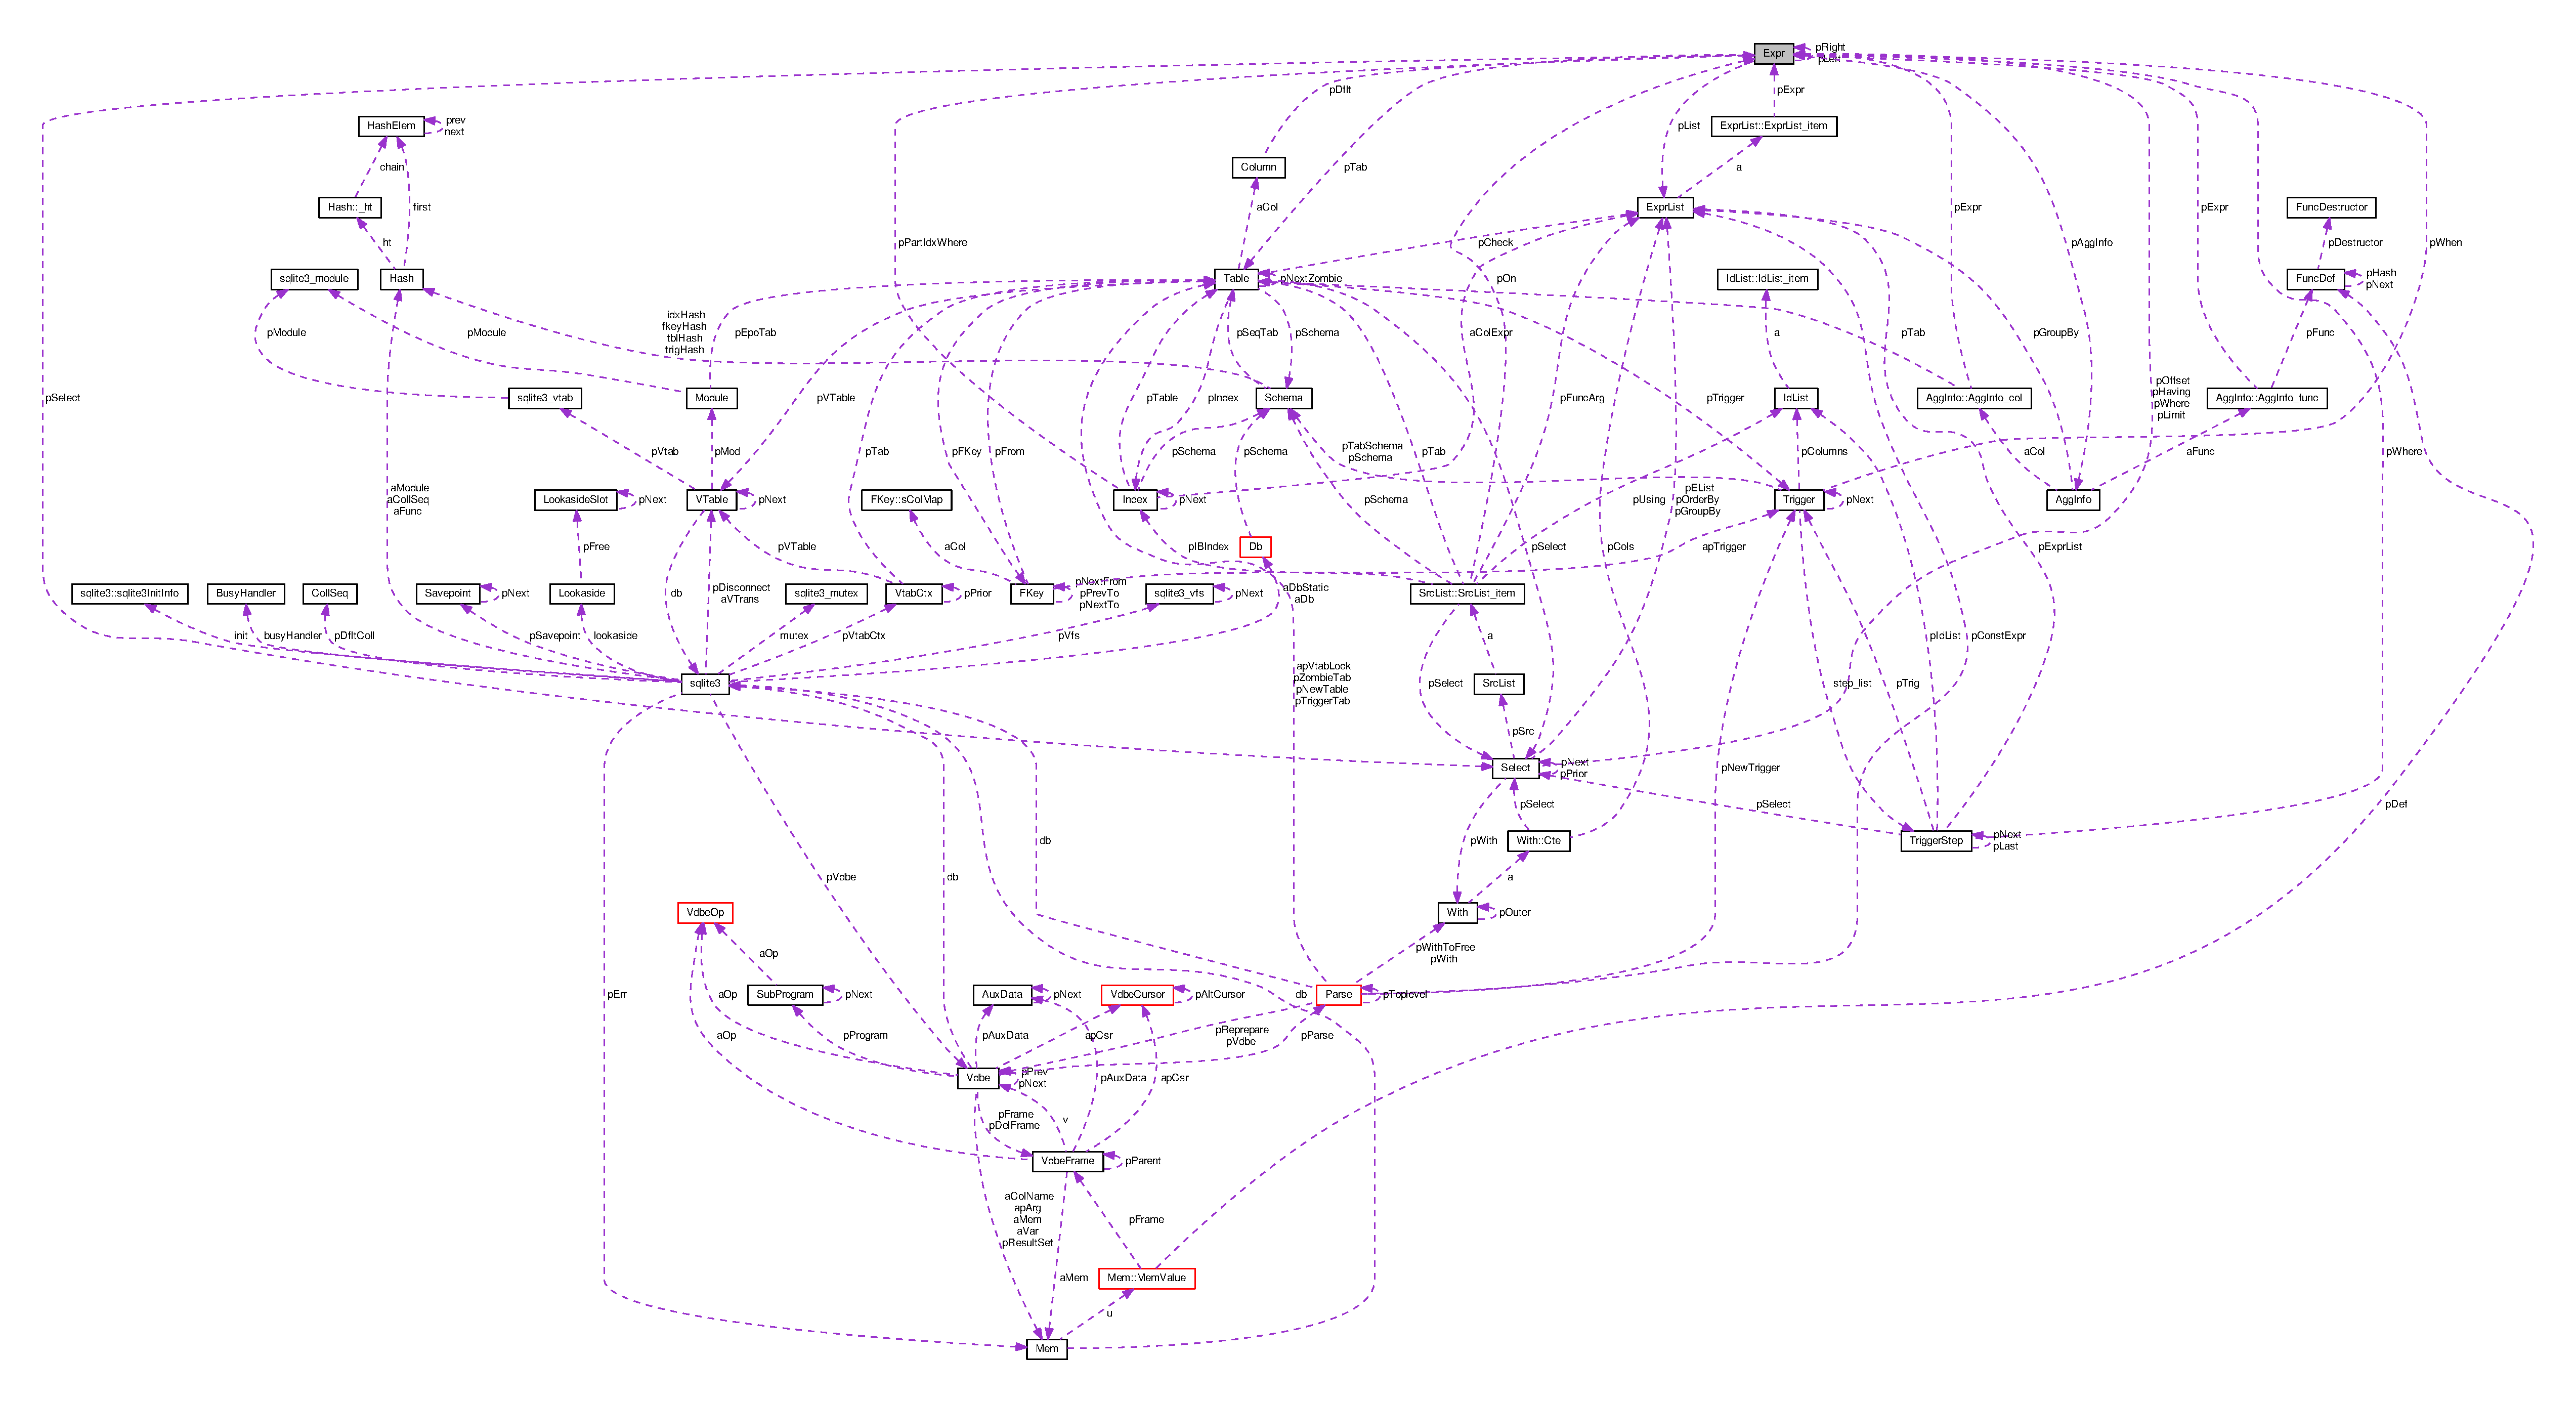
\includegraphics[width=350pt]{structExpr__coll__graph}
\end{center}
\end{figure}
\subsection*{Public Attributes}
\begin{DoxyCompactItemize}
\item 
u8 {\bfseries op}\hypertarget{structExpr_a101c55ddb6c149d95f0327831eb78225}{}\label{structExpr_a101c55ddb6c149d95f0327831eb78225}

\item 
char {\bfseries affinity}\hypertarget{structExpr_aeb51b76e606d6fbae234e38473bf3dc9}{}\label{structExpr_aeb51b76e606d6fbae234e38473bf3dc9}

\item 
u32 {\bfseries flags}\hypertarget{structExpr_aebac9ee7e6aa7adca63969d3ba8d0ded}{}\label{structExpr_aebac9ee7e6aa7adca63969d3ba8d0ded}

\item 
\begin{tabbing}
xx\=xx\=xx\=xx\=xx\=xx\=xx\=xx\=xx\=\kill
union \{\\
\>char $\ast$ {\bfseries zToken}\\
\>int {\bfseries iValue}\\
\} {\bfseries u}\hypertarget{structExpr_a5a43a51aa0ee7afc9babcdc337dd77db}{}\label{structExpr_a5a43a51aa0ee7afc9babcdc337dd77db}
\\

\end{tabbing}\item 
\hyperlink{structExpr}{Expr} $\ast$ {\bfseries p\+Left}\hypertarget{structExpr_a0a78282ae0d696f4a25013a12e38b1ba}{}\label{structExpr_a0a78282ae0d696f4a25013a12e38b1ba}

\item 
\hyperlink{structExpr}{Expr} $\ast$ {\bfseries p\+Right}\hypertarget{structExpr_aa08c218d5b0b6f8882e8bf9ec8822a08}{}\label{structExpr_aa08c218d5b0b6f8882e8bf9ec8822a08}

\item 
\begin{tabbing}
xx\=xx\=xx\=xx\=xx\=xx\=xx\=xx\=xx\=\kill
union \{\\
\>\hyperlink{structExprList}{ExprList} $\ast$ {\bfseries pList}\\
\>\hyperlink{structSelect}{Select} $\ast$ {\bfseries pSelect}\\
\} {\bfseries x}\hypertarget{structExpr_a9ff6313055718299e20a19e551dcbf0a}{}\label{structExpr_a9ff6313055718299e20a19e551dcbf0a}
\\

\end{tabbing}\item 
int {\bfseries n\+Height}\hypertarget{structExpr_a5a893ea309f801f23404e7e5ac02732b}{}\label{structExpr_a5a893ea309f801f23404e7e5ac02732b}

\item 
int {\bfseries i\+Table}\hypertarget{structExpr_af8e273f4d7d173bfb5996ed09054611c}{}\label{structExpr_af8e273f4d7d173bfb5996ed09054611c}

\item 
yn\+Var {\bfseries i\+Column}\hypertarget{structExpr_ad19251a8eb6db3cf0bdffe0dcb07eeba}{}\label{structExpr_ad19251a8eb6db3cf0bdffe0dcb07eeba}

\item 
i16 {\bfseries i\+Agg}\hypertarget{structExpr_a9fe0ed6360b0a4cf5b67ab8def922033}{}\label{structExpr_a9fe0ed6360b0a4cf5b67ab8def922033}

\item 
i16 {\bfseries i\+Right\+Join\+Table}\hypertarget{structExpr_aa49b76f3628a7bf2b0997c33461cc651}{}\label{structExpr_aa49b76f3628a7bf2b0997c33461cc651}

\item 
u8 {\bfseries op2}\hypertarget{structExpr_a0eacba0a2a6977e434b096b1cb9d5b9e}{}\label{structExpr_a0eacba0a2a6977e434b096b1cb9d5b9e}

\item 
\hyperlink{structAggInfo}{Agg\+Info} $\ast$ {\bfseries p\+Agg\+Info}\hypertarget{structExpr_a4fde82477256ee85f3a906263549082a}{}\label{structExpr_a4fde82477256ee85f3a906263549082a}

\item 
\hyperlink{structTable}{Table} $\ast$ {\bfseries p\+Tab}\hypertarget{structExpr_a27c8824b41d853eeeebe61cf3ac1ae5a}{}\label{structExpr_a27c8824b41d853eeeebe61cf3ac1ae5a}

\end{DoxyCompactItemize}


The documentation for this struct was generated from the following file\+:\begin{DoxyCompactItemize}
\item 
sqlite3.\+c\end{DoxyCompactItemize}

\hypertarget{structExprList}{}\section{Expr\+List Struct Reference}
\label{structExprList}\index{Expr\+List@{Expr\+List}}


Collaboration diagram for Expr\+List\+:
% FIG 0
\subsection*{Classes}
\begin{DoxyCompactItemize}
\item 
struct \hyperlink{structExprList_1_1ExprList__item}{Expr\+List\+\_\+item}
\end{DoxyCompactItemize}
\subsection*{Public Attributes}
\begin{DoxyCompactItemize}
\item 
int {\bfseries n\+Expr}\hypertarget{structExprList_a88bdbd62cce306124eea63ae9f80ec33}{}\label{structExprList_a88bdbd62cce306124eea63ae9f80ec33}

\item 
struct \hyperlink{structExprList_1_1ExprList__item}{Expr\+List\+::\+Expr\+List\+\_\+item} $\ast$ {\bfseries a}\hypertarget{structExprList_a02a4222d2dc4da64dcec416188abc16c}{}\label{structExprList_a02a4222d2dc4da64dcec416188abc16c}

\end{DoxyCompactItemize}


The documentation for this struct was generated from the following file\+:\begin{DoxyCompactItemize}
\item 
sqlite3.\+c\end{DoxyCompactItemize}

\hypertarget{structExprList_1_1ExprList__item}{}\section{Expr\+List\+:\+:Expr\+List\+\_\+item Struct Reference}
\label{structExprList_1_1ExprList__item}\index{Expr\+List\+::\+Expr\+List\+\_\+item@{Expr\+List\+::\+Expr\+List\+\_\+item}}


Collaboration diagram for Expr\+List\+:\+:Expr\+List\+\_\+item\+:
% FIG 0
\subsection*{Public Attributes}
\begin{DoxyCompactItemize}
\item 
\hyperlink{structExpr}{Expr} $\ast$ {\bfseries p\+Expr}\hypertarget{structExprList_1_1ExprList__item_a75906cf3ff19e5bf16373fec7f3c79ad}{}\label{structExprList_1_1ExprList__item_a75906cf3ff19e5bf16373fec7f3c79ad}

\item 
char $\ast$ {\bfseries z\+Name}\hypertarget{structExprList_1_1ExprList__item_af278eb03a1169c73d144547adaf9b04f}{}\label{structExprList_1_1ExprList__item_af278eb03a1169c73d144547adaf9b04f}

\item 
char $\ast$ {\bfseries z\+Span}\hypertarget{structExprList_1_1ExprList__item_ade485bb6fafb44ec2aba59d05b8d117b}{}\label{structExprList_1_1ExprList__item_ade485bb6fafb44ec2aba59d05b8d117b}

\item 
u8 {\bfseries sort\+Order}\hypertarget{structExprList_1_1ExprList__item_af9084dc073f96792c0c7a8a894778881}{}\label{structExprList_1_1ExprList__item_af9084dc073f96792c0c7a8a894778881}

\item 
unsigned {\bfseries done}\+:1\hypertarget{structExprList_1_1ExprList__item_a0100abfbd214ec2199dd25e4bce05dcb}{}\label{structExprList_1_1ExprList__item_a0100abfbd214ec2199dd25e4bce05dcb}

\item 
unsigned {\bfseries b\+Span\+Is\+Tab}\+:1\hypertarget{structExprList_1_1ExprList__item_a05e84a6dbbf69cea042d3bf888955999}{}\label{structExprList_1_1ExprList__item_a05e84a6dbbf69cea042d3bf888955999}

\item 
unsigned {\bfseries reusable}\+:1\hypertarget{structExprList_1_1ExprList__item_a066f924fb690e78cd2833770f737a13b}{}\label{structExprList_1_1ExprList__item_a066f924fb690e78cd2833770f737a13b}

\item 
\begin{tabbing}
xx\=xx\=xx\=xx\=xx\=xx\=xx\=xx\=xx\=\kill
union \{\\
\>struct \{\\
\>\>u16 {\bfseries iOrderByCol}\\
\>\>u16 {\bfseries iAlias}\\
\>\} {\bfseries x}\\
\>int {\bfseries iConstExprReg}\\
\} {\bfseries u}\hypertarget{structExprList_1_1ExprList__item_a7bce1eb19061edb080a38a6b826fd789}{}\label{structExprList_1_1ExprList__item_a7bce1eb19061edb080a38a6b826fd789}
\\

\end{tabbing}\end{DoxyCompactItemize}


The documentation for this struct was generated from the following file\+:\begin{DoxyCompactItemize}
\item 
sqlite3.\+c\end{DoxyCompactItemize}

\hypertarget{structExprSpan}{}\section{Expr\+Span Struct Reference}
\label{structExprSpan}\index{Expr\+Span@{Expr\+Span}}


Collaboration diagram for Expr\+Span\+:\nopagebreak
\begin{figure}[H]
\begin{center}
\leavevmode
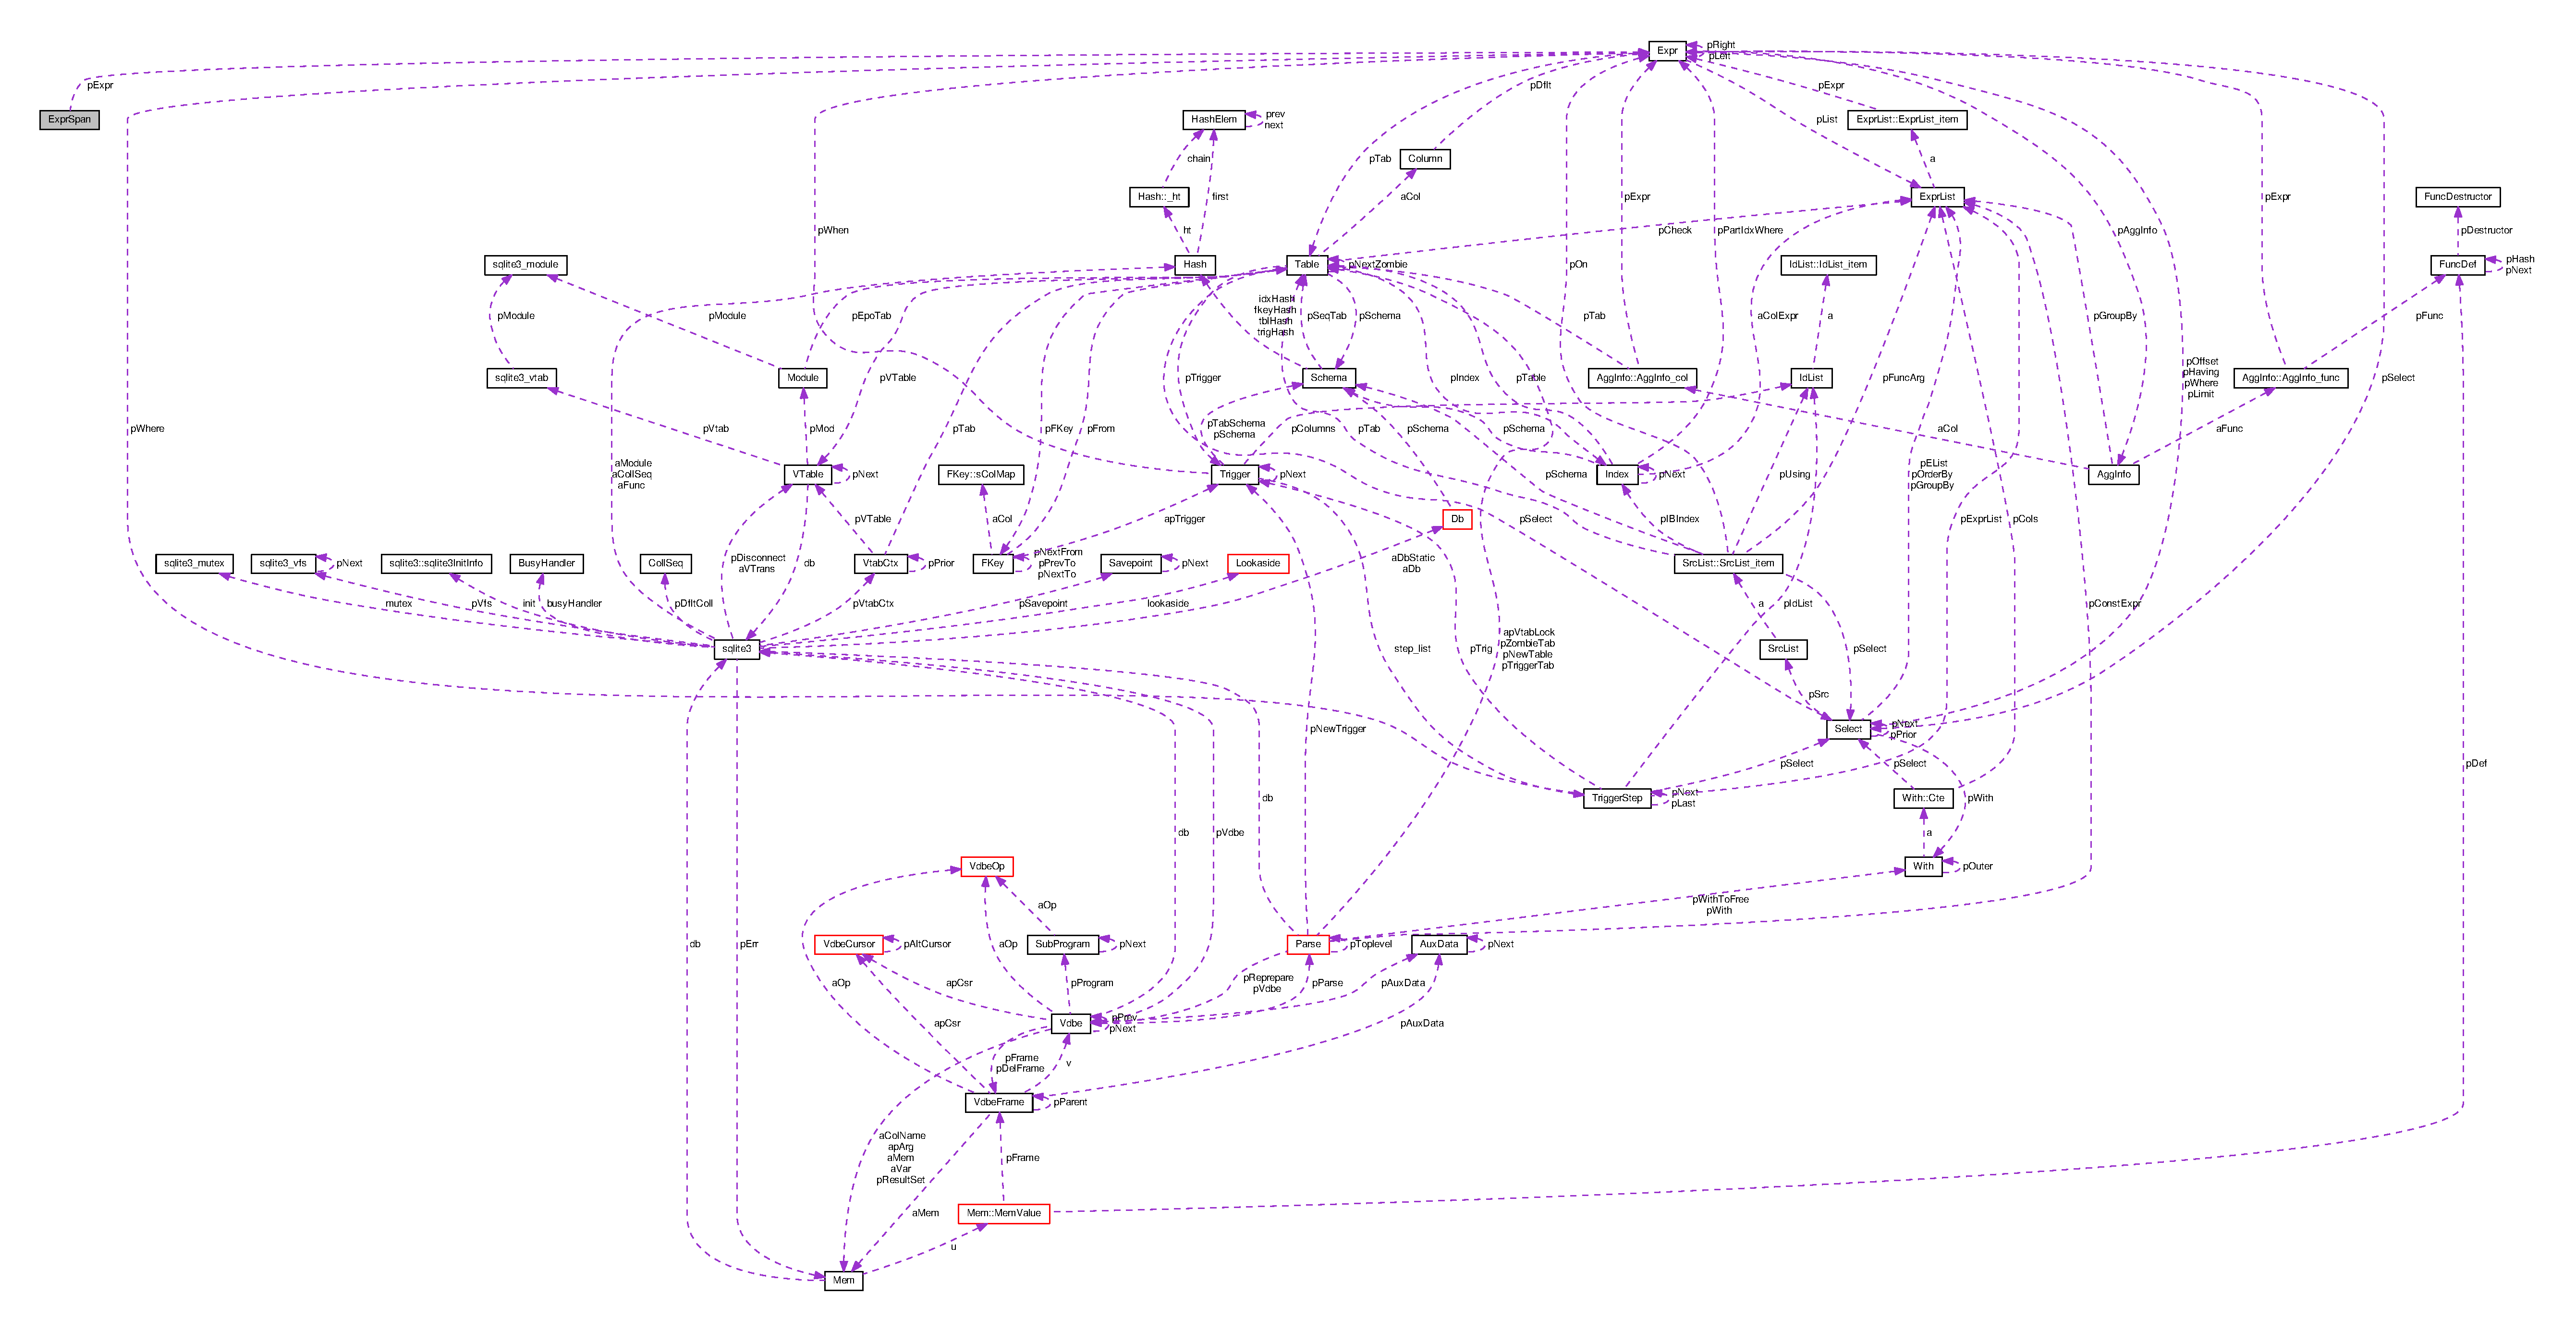
\includegraphics[width=350pt]{structExprSpan__coll__graph}
\end{center}
\end{figure}
\subsection*{Public Attributes}
\begin{DoxyCompactItemize}
\item 
\hyperlink{structExpr}{Expr} $\ast$ {\bfseries p\+Expr}\hypertarget{structExprSpan_a081c4aa031331c8518c1173b2a8335cc}{}\label{structExprSpan_a081c4aa031331c8518c1173b2a8335cc}

\item 
const char $\ast$ {\bfseries z\+Start}\hypertarget{structExprSpan_af4653638d7e67a62e7a607f682b38e25}{}\label{structExprSpan_af4653638d7e67a62e7a607f682b38e25}

\item 
const char $\ast$ {\bfseries z\+End}\hypertarget{structExprSpan_a7cdf42cea729fcb5a1c477c3825ab575}{}\label{structExprSpan_a7cdf42cea729fcb5a1c477c3825ab575}

\end{DoxyCompactItemize}


The documentation for this struct was generated from the following file\+:\begin{DoxyCompactItemize}
\item 
sqlite3.\+c\end{DoxyCompactItemize}

\hypertarget{structFileChunk}{}\section{File\+Chunk Struct Reference}
\label{structFileChunk}\index{File\+Chunk@{File\+Chunk}}


Collaboration diagram for File\+Chunk\+:\nopagebreak
\begin{figure}[H]
\begin{center}
\leavevmode
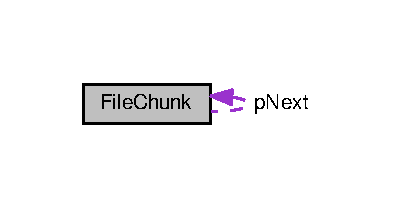
\includegraphics[width=189pt]{structFileChunk__coll__graph}
\end{center}
\end{figure}
\subsection*{Public Attributes}
\begin{DoxyCompactItemize}
\item 
\hyperlink{structFileChunk}{File\+Chunk} $\ast$ {\bfseries p\+Next}\hypertarget{structFileChunk_ad2d0d170afc7ce1e239e8716852e247b}{}\label{structFileChunk_ad2d0d170afc7ce1e239e8716852e247b}

\item 
u8 {\bfseries z\+Chunk} \mbox{[}8\mbox{]}\hypertarget{structFileChunk_a1e7a92812b21bba27661fb38a5f597a7}{}\label{structFileChunk_a1e7a92812b21bba27661fb38a5f597a7}

\end{DoxyCompactItemize}


The documentation for this struct was generated from the following file\+:\begin{DoxyCompactItemize}
\item 
sqlite3.\+c\end{DoxyCompactItemize}

\hypertarget{structFilePoint}{}\section{File\+Point Struct Reference}
\label{structFilePoint}\index{File\+Point@{File\+Point}}


Collaboration diagram for File\+Point\+:\nopagebreak
\begin{figure}[H]
\begin{center}
\leavevmode
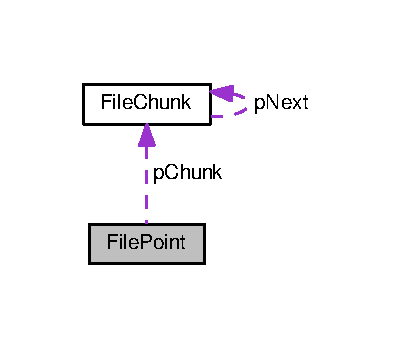
\includegraphics[width=189pt]{structFilePoint__coll__graph}
\end{center}
\end{figure}
\subsection*{Public Attributes}
\begin{DoxyCompactItemize}
\item 
sqlite3\+\_\+int64 {\bfseries i\+Offset}\hypertarget{structFilePoint_a00a345e479cd37ebeb9e6ed475eb4112}{}\label{structFilePoint_a00a345e479cd37ebeb9e6ed475eb4112}

\item 
\hyperlink{structFileChunk}{File\+Chunk} $\ast$ {\bfseries p\+Chunk}\hypertarget{structFilePoint_aa17216d9d2559f14a00a2c72a8959298}{}\label{structFilePoint_aa17216d9d2559f14a00a2c72a8959298}

\end{DoxyCompactItemize}


The documentation for this struct was generated from the following file\+:\begin{DoxyCompactItemize}
\item 
sqlite3.\+c\end{DoxyCompactItemize}

\hypertarget{structFKey}{}\section{F\+Key Struct Reference}
\label{structFKey}\index{F\+Key@{F\+Key}}


Collaboration diagram for F\+Key\+:
% FIG 0
\subsection*{Classes}
\begin{DoxyCompactItemize}
\item 
struct \hyperlink{structFKey_1_1sColMap}{s\+Col\+Map}
\end{DoxyCompactItemize}
\subsection*{Public Attributes}
\begin{DoxyCompactItemize}
\item 
\hyperlink{structTable}{Table} $\ast$ {\bfseries p\+From}\hypertarget{structFKey_a6d476f3fbfa75a19c5c5a9edec4e79eb}{}\label{structFKey_a6d476f3fbfa75a19c5c5a9edec4e79eb}

\item 
\hyperlink{structFKey}{F\+Key} $\ast$ {\bfseries p\+Next\+From}\hypertarget{structFKey_ac64ff66b30167715c8822a74c2809075}{}\label{structFKey_ac64ff66b30167715c8822a74c2809075}

\item 
char $\ast$ {\bfseries z\+To}\hypertarget{structFKey_a1eac10bab38a0ac9f88306fbbabbe5d6}{}\label{structFKey_a1eac10bab38a0ac9f88306fbbabbe5d6}

\item 
\hyperlink{structFKey}{F\+Key} $\ast$ {\bfseries p\+Next\+To}\hypertarget{structFKey_ac29b26999113602e7e3921bf07643c04}{}\label{structFKey_ac29b26999113602e7e3921bf07643c04}

\item 
\hyperlink{structFKey}{F\+Key} $\ast$ {\bfseries p\+Prev\+To}\hypertarget{structFKey_a56189e420e91df86513e6895db518eca}{}\label{structFKey_a56189e420e91df86513e6895db518eca}

\item 
int {\bfseries n\+Col}\hypertarget{structFKey_a611e3223f3f434e0a635e036dc100cbb}{}\label{structFKey_a611e3223f3f434e0a635e036dc100cbb}

\item 
u8 {\bfseries is\+Deferred}\hypertarget{structFKey_ab742714b17f2c13353837e1fdde51cc7}{}\label{structFKey_ab742714b17f2c13353837e1fdde51cc7}

\item 
u8 {\bfseries a\+Action} \mbox{[}2\mbox{]}\hypertarget{structFKey_a68a08f58294bf845e9c77d785499d222}{}\label{structFKey_a68a08f58294bf845e9c77d785499d222}

\item 
\hyperlink{structTrigger}{Trigger} $\ast$ {\bfseries ap\+Trigger} \mbox{[}2\mbox{]}\hypertarget{structFKey_a9ce15cb27b675836bc714ab18fd8a008}{}\label{structFKey_a9ce15cb27b675836bc714ab18fd8a008}

\item 
struct \hyperlink{structFKey_1_1sColMap}{F\+Key\+::s\+Col\+Map} {\bfseries a\+Col} \mbox{[}1\mbox{]}\hypertarget{structFKey_a5b230bc6c10a67f432ed7d5ebc92bcd2}{}\label{structFKey_a5b230bc6c10a67f432ed7d5ebc92bcd2}

\end{DoxyCompactItemize}


The documentation for this struct was generated from the following file\+:\begin{DoxyCompactItemize}
\item 
sqlite3.\+c\end{DoxyCompactItemize}

\hypertarget{structfts5__api}{}\section{fts5\+\_\+api Struct Reference}
\label{structfts5__api}\index{fts5\+\_\+api@{fts5\+\_\+api}}
\subsection*{Public Attributes}
\begin{DoxyCompactItemize}
\item 
int {\bfseries i\+Version}\hypertarget{structfts5__api_a3c338289abb33e1805da870172956a7c}{}\label{structfts5__api_a3c338289abb33e1805da870172956a7c}

\item 
int($\ast$ {\bfseries x\+Create\+Tokenizer} )(\hyperlink{structfts5__api}{fts5\+\_\+api} $\ast$p\+Api, const char $\ast$z\+Name, void $\ast$p\+Context, \hyperlink{structfts5__tokenizer}{fts5\+\_\+tokenizer} $\ast$p\+Tokenizer, void($\ast$x\+Destroy)(void $\ast$))\hypertarget{structfts5__api_a6cb9929558ff13c7b5a30292eb5aea7c}{}\label{structfts5__api_a6cb9929558ff13c7b5a30292eb5aea7c}

\item 
int($\ast$ {\bfseries x\+Find\+Tokenizer} )(\hyperlink{structfts5__api}{fts5\+\_\+api} $\ast$p\+Api, const char $\ast$z\+Name, void $\ast$$\ast$pp\+Context, \hyperlink{structfts5__tokenizer}{fts5\+\_\+tokenizer} $\ast$p\+Tokenizer)\hypertarget{structfts5__api_aa232f72a0d7c7205fbd0dc6818e24aee}{}\label{structfts5__api_aa232f72a0d7c7205fbd0dc6818e24aee}

\item 
int($\ast$ {\bfseries x\+Create\+Function} )(\hyperlink{structfts5__api}{fts5\+\_\+api} $\ast$p\+Api, const char $\ast$z\+Name, void $\ast$p\+Context, fts5\+\_\+extension\+\_\+function x\+Function, void($\ast$x\+Destroy)(void $\ast$))\hypertarget{structfts5__api_aa932ba45865c10b49592920b9610db93}{}\label{structfts5__api_aa932ba45865c10b49592920b9610db93}

\end{DoxyCompactItemize}


The documentation for this struct was generated from the following files\+:\begin{DoxyCompactItemize}
\item 
sqlite3.\+c\item 
sqlite3.\+h\end{DoxyCompactItemize}

\hypertarget{structfts5__tokenizer}{}\section{fts5\+\_\+tokenizer Struct Reference}
\label{structfts5__tokenizer}\index{fts5\+\_\+tokenizer@{fts5\+\_\+tokenizer}}
\subsection*{Public Attributes}
\begin{DoxyCompactItemize}
\item 
int($\ast$ {\bfseries x\+Create} )(void $\ast$, const char $\ast$$\ast$az\+Arg, int n\+Arg, Fts5\+Tokenizer $\ast$$\ast$pp\+Out)\hypertarget{structfts5__tokenizer_ab0e73328047d3191668ecad51839873d}{}\label{structfts5__tokenizer_ab0e73328047d3191668ecad51839873d}

\item 
void($\ast$ {\bfseries x\+Delete} )(Fts5\+Tokenizer $\ast$)\hypertarget{structfts5__tokenizer_a5df6926b15f5ccbffdcdf635f2f76142}{}\label{structfts5__tokenizer_a5df6926b15f5ccbffdcdf635f2f76142}

\item 
int($\ast$ {\bfseries x\+Tokenize} )(Fts5\+Tokenizer $\ast$, void $\ast$p\+Ctx, int flags, const char $\ast$p\+Text, int n\+Text, int($\ast$x\+Token)(                       void $\ast$p\+Ctx,                           
                       int tflags,                           
                       const char $\ast$p\+Token,                       int n\+Token,                           
                       int i\+Start,                           
                       int i\+End                                       
               ))\hypertarget{structfts5__tokenizer_a7e4fce365700c8e3801c5dc6f7f2d064}{}\label{structfts5__tokenizer_a7e4fce365700c8e3801c5dc6f7f2d064}

\end{DoxyCompactItemize}


The documentation for this struct was generated from the following files\+:\begin{DoxyCompactItemize}
\item 
sqlite3.\+c\item 
sqlite3.\+h\end{DoxyCompactItemize}

\hypertarget{structFts5ExtensionApi}{}\section{Fts5\+Extension\+Api Struct Reference}
\label{structFts5ExtensionApi}\index{Fts5\+Extension\+Api@{Fts5\+Extension\+Api}}
\subsection*{Public Attributes}
\begin{DoxyCompactItemize}
\item 
int {\bfseries i\+Version}\hypertarget{structFts5ExtensionApi_af9c8f09c2e6f1373e6bce57ec9861682}{}\label{structFts5ExtensionApi_af9c8f09c2e6f1373e6bce57ec9861682}

\item 
void $\ast$($\ast$ {\bfseries x\+User\+Data} )(Fts5\+Context $\ast$)\hypertarget{structFts5ExtensionApi_a1f71f2622761df6f157e7201879bf5df}{}\label{structFts5ExtensionApi_a1f71f2622761df6f157e7201879bf5df}

\item 
int($\ast$ {\bfseries x\+Column\+Count} )(Fts5\+Context $\ast$)\hypertarget{structFts5ExtensionApi_a33c1e050aa9e9b746205c192935f4a1d}{}\label{structFts5ExtensionApi_a33c1e050aa9e9b746205c192935f4a1d}

\item 
int($\ast$ {\bfseries x\+Row\+Count} )(Fts5\+Context $\ast$, sqlite3\+\_\+int64 $\ast$pn\+Row)\hypertarget{structFts5ExtensionApi_a7f82e336e97540cb7efb66bd27042e4f}{}\label{structFts5ExtensionApi_a7f82e336e97540cb7efb66bd27042e4f}

\item 
int($\ast$ {\bfseries x\+Column\+Total\+Size} )(Fts5\+Context $\ast$, int i\+Col, sqlite3\+\_\+int64 $\ast$pn\+Token)\hypertarget{structFts5ExtensionApi_acfc4e9d9879578a4b9347d7876d28963}{}\label{structFts5ExtensionApi_acfc4e9d9879578a4b9347d7876d28963}

\item 
int($\ast$ {\bfseries x\+Tokenize} )(Fts5\+Context $\ast$, const char $\ast$p\+Text, int n\+Text, void $\ast$p\+Ctx, int($\ast$x\+Token)(void $\ast$, int, const char $\ast$, int, int, int))\hypertarget{structFts5ExtensionApi_ae10d6563d3adc047eaba8db50eea1762}{}\label{structFts5ExtensionApi_ae10d6563d3adc047eaba8db50eea1762}

\item 
int($\ast$ {\bfseries x\+Phrase\+Count} )(Fts5\+Context $\ast$)\hypertarget{structFts5ExtensionApi_a79916567d32f1933bb98d5939b8e0885}{}\label{structFts5ExtensionApi_a79916567d32f1933bb98d5939b8e0885}

\item 
int($\ast$ {\bfseries x\+Phrase\+Size} )(Fts5\+Context $\ast$, int i\+Phrase)\hypertarget{structFts5ExtensionApi_a35442bdd54fd59f3a0d0eab74df50571}{}\label{structFts5ExtensionApi_a35442bdd54fd59f3a0d0eab74df50571}

\item 
int($\ast$ {\bfseries x\+Inst\+Count} )(Fts5\+Context $\ast$, int $\ast$pn\+Inst)\hypertarget{structFts5ExtensionApi_a4095d1d4a90ee27fe3586b4dcca16151}{}\label{structFts5ExtensionApi_a4095d1d4a90ee27fe3586b4dcca16151}

\item 
int($\ast$ {\bfseries x\+Inst} )(Fts5\+Context $\ast$, int i\+Idx, int $\ast$pi\+Phrase, int $\ast$pi\+Col, int $\ast$pi\+Off)\hypertarget{structFts5ExtensionApi_af2f1796923ab2d48be770e860e7494cb}{}\label{structFts5ExtensionApi_af2f1796923ab2d48be770e860e7494cb}

\item 
sqlite3\+\_\+int64($\ast$ {\bfseries x\+Rowid} )(Fts5\+Context $\ast$)\hypertarget{structFts5ExtensionApi_aab4c236653ae8b3d1f306fc7af5c7ed1}{}\label{structFts5ExtensionApi_aab4c236653ae8b3d1f306fc7af5c7ed1}

\item 
int($\ast$ {\bfseries x\+Column\+Text} )(Fts5\+Context $\ast$, int i\+Col, const char $\ast$$\ast$pz, int $\ast$pn)\hypertarget{structFts5ExtensionApi_af1aedeaa82104e3e0495ed22610ad4bc}{}\label{structFts5ExtensionApi_af1aedeaa82104e3e0495ed22610ad4bc}

\item 
int($\ast$ {\bfseries x\+Column\+Size} )(Fts5\+Context $\ast$, int i\+Col, int $\ast$pn\+Token)\hypertarget{structFts5ExtensionApi_ad1e249d1ce89ac0b05b77ea32a4da0cd}{}\label{structFts5ExtensionApi_ad1e249d1ce89ac0b05b77ea32a4da0cd}

\item 
int($\ast$ {\bfseries x\+Query\+Phrase} )(Fts5\+Context $\ast$, int i\+Phrase, void $\ast$p\+User\+Data, int($\ast$)(const \hyperlink{structFts5ExtensionApi}{Fts5\+Extension\+Api} $\ast$, Fts5\+Context $\ast$, void $\ast$))\hypertarget{structFts5ExtensionApi_a66af7d07783c18b2c59025f982b2bd92}{}\label{structFts5ExtensionApi_a66af7d07783c18b2c59025f982b2bd92}

\item 
int($\ast$ {\bfseries x\+Set\+Auxdata} )(Fts5\+Context $\ast$, void $\ast$p\+Aux, void($\ast$x\+Delete)(void $\ast$))\hypertarget{structFts5ExtensionApi_a466af4264428f467ee94408b64f408cb}{}\label{structFts5ExtensionApi_a466af4264428f467ee94408b64f408cb}

\item 
void $\ast$($\ast$ {\bfseries x\+Get\+Auxdata} )(Fts5\+Context $\ast$, int b\+Clear)\hypertarget{structFts5ExtensionApi_ab18b1cb62e84590f50c0e007366165fb}{}\label{structFts5ExtensionApi_ab18b1cb62e84590f50c0e007366165fb}

\item 
int($\ast$ {\bfseries x\+Phrase\+First} )(Fts5\+Context $\ast$, int i\+Phrase, \hyperlink{structFts5PhraseIter}{Fts5\+Phrase\+Iter} $\ast$, int $\ast$, int $\ast$)\hypertarget{structFts5ExtensionApi_a0e7fb192d7ca28a5cc4f9ef025586761}{}\label{structFts5ExtensionApi_a0e7fb192d7ca28a5cc4f9ef025586761}

\item 
void($\ast$ {\bfseries x\+Phrase\+Next} )(Fts5\+Context $\ast$, \hyperlink{structFts5PhraseIter}{Fts5\+Phrase\+Iter} $\ast$, int $\ast$pi\+Col, int $\ast$pi\+Off)\hypertarget{structFts5ExtensionApi_a049c7163a39f20c675cf261fa181a9a1}{}\label{structFts5ExtensionApi_a049c7163a39f20c675cf261fa181a9a1}

\item 
int($\ast$ {\bfseries x\+Phrase\+First\+Column} )(Fts5\+Context $\ast$, int i\+Phrase, \hyperlink{structFts5PhraseIter}{Fts5\+Phrase\+Iter} $\ast$, int $\ast$)\hypertarget{structFts5ExtensionApi_ac1936193fd724dd4cac4772add9a724b}{}\label{structFts5ExtensionApi_ac1936193fd724dd4cac4772add9a724b}

\item 
void($\ast$ {\bfseries x\+Phrase\+Next\+Column} )(Fts5\+Context $\ast$, \hyperlink{structFts5PhraseIter}{Fts5\+Phrase\+Iter} $\ast$, int $\ast$pi\+Col)\hypertarget{structFts5ExtensionApi_aab6694c0e06fc2a5ecca0041a492f2b1}{}\label{structFts5ExtensionApi_aab6694c0e06fc2a5ecca0041a492f2b1}

\end{DoxyCompactItemize}


The documentation for this struct was generated from the following files\+:\begin{DoxyCompactItemize}
\item 
sqlite3.\+c\item 
sqlite3.\+h\end{DoxyCompactItemize}

\hypertarget{structFts5PhraseIter}{}\section{Fts5\+Phrase\+Iter Struct Reference}
\label{structFts5PhraseIter}\index{Fts5\+Phrase\+Iter@{Fts5\+Phrase\+Iter}}
\subsection*{Public Attributes}
\begin{DoxyCompactItemize}
\item 
const unsigned char $\ast$ {\bfseries a}\hypertarget{structFts5PhraseIter_ae7989e86f7246b1edf3f090867ae0604}{}\label{structFts5PhraseIter_ae7989e86f7246b1edf3f090867ae0604}

\item 
const unsigned char $\ast$ {\bfseries b}\hypertarget{structFts5PhraseIter_ac783edf6256522bd2a48a35bee957327}{}\label{structFts5PhraseIter_ac783edf6256522bd2a48a35bee957327}

\end{DoxyCompactItemize}


The documentation for this struct was generated from the following files\+:\begin{DoxyCompactItemize}
\item 
sqlite3.\+c\item 
sqlite3.\+h\end{DoxyCompactItemize}

\hypertarget{structFuncDef}{}\section{Func\+Def Struct Reference}
\label{structFuncDef}\index{Func\+Def@{Func\+Def}}


Collaboration diagram for Func\+Def\+:
% FIG 0
\subsection*{Public Attributes}
\begin{DoxyCompactItemize}
\item 
i8 {\bfseries n\+Arg}\hypertarget{structFuncDef_a65d2af5dc68a0344efb368b8ce1b9141}{}\label{structFuncDef_a65d2af5dc68a0344efb368b8ce1b9141}

\item 
u16 {\bfseries func\+Flags}\hypertarget{structFuncDef_a4cd12fdb0da08ec8a5fb41f8bcd09e78}{}\label{structFuncDef_a4cd12fdb0da08ec8a5fb41f8bcd09e78}

\item 
void $\ast$ {\bfseries p\+User\+Data}\hypertarget{structFuncDef_a04fdde2f96be198823a483bebcfd3ae3}{}\label{structFuncDef_a04fdde2f96be198823a483bebcfd3ae3}

\item 
\hyperlink{structFuncDef}{Func\+Def} $\ast$ {\bfseries p\+Next}\hypertarget{structFuncDef_a1ebe547d000172d9ae44d12eeb433a48}{}\label{structFuncDef_a1ebe547d000172d9ae44d12eeb433a48}

\item 
void($\ast$ {\bfseries x\+S\+Func} )(\hyperlink{structsqlite3__context}{sqlite3\+\_\+context} $\ast$, int, \hyperlink{structMem}{sqlite3\+\_\+value} $\ast$$\ast$)\hypertarget{structFuncDef_a64986fd7c3b2a3715f5e7a54c0ef385e}{}\label{structFuncDef_a64986fd7c3b2a3715f5e7a54c0ef385e}

\item 
void($\ast$ {\bfseries x\+Finalize} )(\hyperlink{structsqlite3__context}{sqlite3\+\_\+context} $\ast$)\hypertarget{structFuncDef_a2315fa9b1a173dca2ba0c506548b83f9}{}\label{structFuncDef_a2315fa9b1a173dca2ba0c506548b83f9}

\item 
const char $\ast$ {\bfseries z\+Name}\hypertarget{structFuncDef_ac732c25b31e5c5a5390db76e74724024}{}\label{structFuncDef_ac732c25b31e5c5a5390db76e74724024}

\item 
\begin{tabbing}
xx\=xx\=xx\=xx\=xx\=xx\=xx\=xx\=xx\=\kill
union \{\\
\>\hyperlink{structFuncDef}{FuncDef} $\ast$ {\bfseries pHash}\\
\>\hyperlink{structFuncDestructor}{FuncDestructor} $\ast$ {\bfseries pDestructor}\\
\} {\bfseries u}\hypertarget{structFuncDef_a0ed4a95c4ba5c803bfe7adf48888c2dd}{}\label{structFuncDef_a0ed4a95c4ba5c803bfe7adf48888c2dd}
\\

\end{tabbing}\end{DoxyCompactItemize}


The documentation for this struct was generated from the following file\+:\begin{DoxyCompactItemize}
\item 
sqlite3.\+c\end{DoxyCompactItemize}

\hypertarget{structFuncDefHash}{}\section{Func\+Def\+Hash Struct Reference}
\label{structFuncDefHash}\index{Func\+Def\+Hash@{Func\+Def\+Hash}}


Collaboration diagram for Func\+Def\+Hash\+:\nopagebreak
\begin{figure}[H]
\begin{center}
\leavevmode
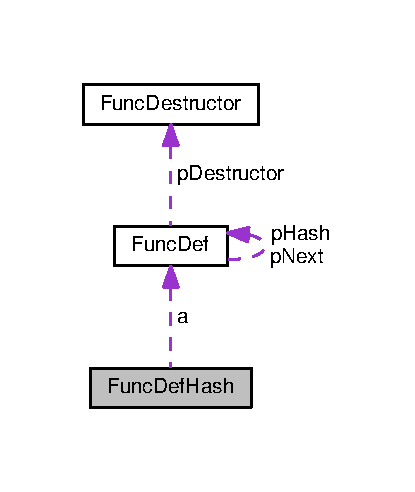
\includegraphics[width=199pt]{structFuncDefHash__coll__graph}
\end{center}
\end{figure}
\subsection*{Public Attributes}
\begin{DoxyCompactItemize}
\item 
\hyperlink{structFuncDef}{Func\+Def} $\ast$ {\bfseries a} \mbox{[}S\+Q\+L\+I\+T\+E\+\_\+\+F\+U\+N\+C\+\_\+\+H\+A\+S\+H\+\_\+\+SZ\mbox{]}\hypertarget{structFuncDefHash_aaab2cd9c5f40d92c236f8fdeb2d9849a}{}\label{structFuncDefHash_aaab2cd9c5f40d92c236f8fdeb2d9849a}

\end{DoxyCompactItemize}


The documentation for this struct was generated from the following file\+:\begin{DoxyCompactItemize}
\item 
sqlite3.\+c\end{DoxyCompactItemize}

\hypertarget{structFuncDestructor}{}\section{Func\+Destructor Struct Reference}
\label{structFuncDestructor}\index{Func\+Destructor@{Func\+Destructor}}
\subsection*{Public Attributes}
\begin{DoxyCompactItemize}
\item 
int {\bfseries n\+Ref}\hypertarget{structFuncDestructor_a8b1bf3af00c88400efc1dd74a4410463}{}\label{structFuncDestructor_a8b1bf3af00c88400efc1dd74a4410463}

\item 
void($\ast$ {\bfseries x\+Destroy} )(void $\ast$)\hypertarget{structFuncDestructor_a53c33a1ad567b79570c783a8a65d6246}{}\label{structFuncDestructor_a53c33a1ad567b79570c783a8a65d6246}

\item 
void $\ast$ {\bfseries p\+User\+Data}\hypertarget{structFuncDestructor_a181875609f0f8221985cd6cfd7ad8cd8}{}\label{structFuncDestructor_a181875609f0f8221985cd6cfd7ad8cd8}

\end{DoxyCompactItemize}


The documentation for this struct was generated from the following file\+:\begin{DoxyCompactItemize}
\item 
sqlite3.\+c\end{DoxyCompactItemize}

\hypertarget{classGenetic}{}\section{Genetic Class Reference}
\label{classGenetic}\index{Genetic@{Genetic}}
\subsection*{Public Member Functions}
\begin{DoxyCompactItemize}
\item 
\hyperlink{classGenetic_a459e4673eb23cb59264140f952f67517}{Genetic} (vector$<$ \hyperlink{classPackage}{Package} $\ast$ $>$ $\ast$packs, vector$<$ vector$<$ unsigned int $>$ $>$ $\ast$matrix, unsigned int weight, unsigned int pack\+Limit, unsigned int population, float stops, float drive)\hypertarget{classGenetic_a459e4673eb23cb59264140f952f67517}{}\label{classGenetic_a459e4673eb23cb59264140f952f67517}

\begin{DoxyCompactList}\small\item\em Default constructor $\ast$/. \end{DoxyCompactList}\item 
virtual \hyperlink{classGenetic_a1a441ff7125fb70aeb0ad279474af9a6}{$\sim$\+Genetic} ()\hypertarget{classGenetic_a1a441ff7125fb70aeb0ad279474af9a6}{}\label{classGenetic_a1a441ff7125fb70aeb0ad279474af9a6}

\begin{DoxyCompactList}\small\item\em Default destructor $\ast$/. \end{DoxyCompactList}\item 
void {\bfseries init\+Population} ()\hypertarget{classGenetic_a8fc0ba91c031e9606a63bee4efa15fd9}{}\label{classGenetic_a8fc0ba91c031e9606a63bee4efa15fd9}

\item 
float {\bfseries fitness} (vector$<$ \hyperlink{classClient}{Client} $\ast$ $>$)\hypertarget{classGenetic_a93e3fd37c5ea87fe2d5189387ff813b8}{}\label{classGenetic_a93e3fd37c5ea87fe2d5189387ff813b8}

\end{DoxyCompactItemize}
\subsection*{Private Attributes}
\begin{DoxyCompactItemize}
\item 
vector$<$ \hyperlink{classPackage}{Package} $\ast$ $>$ $\ast$ {\bfseries packages}\hypertarget{classGenetic_a5e98b22c206236130ab041dc7a8221b3}{}\label{classGenetic_a5e98b22c206236130ab041dc7a8221b3}

\item 
vector$<$ vector$<$ unsigned int $>$ $>$ $\ast$ {\bfseries ad\+Matrix}\hypertarget{classGenetic_a2941366d1afb2f0d9256909ca30a601f}{}\label{classGenetic_a2941366d1afb2f0d9256909ca30a601f}

\item 
unsigned int {\bfseries pop\+Num}\hypertarget{classGenetic_a644a04082c893bfecba4b60e6c881dcd}{}\label{classGenetic_a644a04082c893bfecba4b60e6c881dcd}

\item 
unsigned int {\bfseries weight\+Limit}\hypertarget{classGenetic_a4545405d58dd365147d709dcc4e7bb0a}{}\label{classGenetic_a4545405d58dd365147d709dcc4e7bb0a}

\item 
unsigned int {\bfseries package\+Limit}\hypertarget{classGenetic_a0360729e64ff5021ceae7019c44feee4}{}\label{classGenetic_a0360729e64ff5021ceae7019c44feee4}

\item 
float {\bfseries stop\+Time}\hypertarget{classGenetic_a52276cb3e4b3e5c5423c9747a3ea5631}{}\label{classGenetic_a52276cb3e4b3e5c5423c9747a3ea5631}

\item 
float {\bfseries drive\+Time}\hypertarget{classGenetic_a060cb30bbd912dd78fbf567410746631}{}\label{classGenetic_a060cb30bbd912dd78fbf567410746631}

\item 
vector$<$ vector$<$ \hyperlink{classClient}{Client} $\ast$ $>$ $>$ {\bfseries genes}\hypertarget{classGenetic_a534fa331449d7b496e799bd2b505eea6}{}\label{classGenetic_a534fa331449d7b496e799bd2b505eea6}

\item 
vector$<$ \hyperlink{classClient}{Client} $\ast$ $>$ {\bfseries best\+Fit}\hypertarget{classGenetic_a3024d7bb48ec1034f5baa753dfcf1597}{}\label{classGenetic_a3024d7bb48ec1034f5baa753dfcf1597}

\end{DoxyCompactItemize}


The documentation for this class was generated from the following files\+:\begin{DoxyCompactItemize}
\item 
Genetic.\+h\item 
Genetic.\+cpp\end{DoxyCompactItemize}

\hypertarget{structHash}{}\section{Hash Struct Reference}
\label{structHash}\index{Hash@{Hash}}


Collaboration diagram for Hash\+:
% FIG 0
\subsection*{Classes}
\begin{DoxyCompactItemize}
\item 
struct \hyperlink{structHash_1_1__ht}{\+\_\+ht}
\end{DoxyCompactItemize}
\subsection*{Public Attributes}
\begin{DoxyCompactItemize}
\item 
unsigned int {\bfseries htsize}\hypertarget{structHash_a072258e24a38e09175f1308deb013bc8}{}\label{structHash_a072258e24a38e09175f1308deb013bc8}

\item 
unsigned int {\bfseries count}\hypertarget{structHash_a7ab16f173cdc347ffbe39eaa85ee6fda}{}\label{structHash_a7ab16f173cdc347ffbe39eaa85ee6fda}

\item 
\hyperlink{structHashElem}{Hash\+Elem} $\ast$ {\bfseries first}\hypertarget{structHash_a2cfc9936ca2a624c6492ab6557f4705b}{}\label{structHash_a2cfc9936ca2a624c6492ab6557f4705b}

\item 
struct \hyperlink{structHash_1_1__ht}{Hash\+::\+\_\+ht} $\ast$ {\bfseries ht}\hypertarget{structHash_ac0f36e03746a3fe69643db08d93bc0c4}{}\label{structHash_ac0f36e03746a3fe69643db08d93bc0c4}

\end{DoxyCompactItemize}


The documentation for this struct was generated from the following file\+:\begin{DoxyCompactItemize}
\item 
sqlite3.\+c\end{DoxyCompactItemize}

\hypertarget{structHashElem}{}\section{Hash\+Elem Struct Reference}
\label{structHashElem}\index{Hash\+Elem@{Hash\+Elem}}


Collaboration diagram for Hash\+Elem\+:
% FIG 0
\subsection*{Public Attributes}
\begin{DoxyCompactItemize}
\item 
\hyperlink{structHashElem}{Hash\+Elem} $\ast$ {\bfseries next}\hypertarget{structHashElem_a2d28fad45ff21ffb8a02a7133df860fd}{}\label{structHashElem_a2d28fad45ff21ffb8a02a7133df860fd}

\item 
\hyperlink{structHashElem}{Hash\+Elem} $\ast$ {\bfseries prev}\hypertarget{structHashElem_ae4d011c0dc807a3c100ccdb927dd0ba9}{}\label{structHashElem_ae4d011c0dc807a3c100ccdb927dd0ba9}

\item 
void $\ast$ {\bfseries data}\hypertarget{structHashElem_ac7e80f63ba2f82457ff68aa0cd360365}{}\label{structHashElem_ac7e80f63ba2f82457ff68aa0cd360365}

\item 
const char $\ast$ {\bfseries p\+Key}\hypertarget{structHashElem_a9c33a7c8ac467a5547a123338daf61f4}{}\label{structHashElem_a9c33a7c8ac467a5547a123338daf61f4}

\end{DoxyCompactItemize}


The documentation for this struct was generated from the following file\+:\begin{DoxyCompactItemize}
\item 
sqlite3.\+c\end{DoxyCompactItemize}

\hypertarget{structIdList}{}\section{Id\+List Struct Reference}
\label{structIdList}\index{Id\+List@{Id\+List}}


Collaboration diagram for Id\+List\+:
% FIG 0
\subsection*{Classes}
\begin{DoxyCompactItemize}
\item 
struct \hyperlink{structIdList_1_1IdList__item}{Id\+List\+\_\+item}
\end{DoxyCompactItemize}
\subsection*{Public Attributes}
\begin{DoxyCompactItemize}
\item 
struct \hyperlink{structIdList_1_1IdList__item}{Id\+List\+::\+Id\+List\+\_\+item} $\ast$ {\bfseries a}\hypertarget{structIdList_ad33082fd71286c1159711a1a3e979763}{}\label{structIdList_ad33082fd71286c1159711a1a3e979763}

\item 
int {\bfseries n\+Id}\hypertarget{structIdList_afb785717796d8b3c72d1ae682dcb6ff0}{}\label{structIdList_afb785717796d8b3c72d1ae682dcb6ff0}

\end{DoxyCompactItemize}


The documentation for this struct was generated from the following file\+:\begin{DoxyCompactItemize}
\item 
sqlite3.\+c\end{DoxyCompactItemize}

\hypertarget{structIdList_1_1IdList__item}{}\section{Id\+List\+:\+:Id\+List\+\_\+item Struct Reference}
\label{structIdList_1_1IdList__item}\index{Id\+List\+::\+Id\+List\+\_\+item@{Id\+List\+::\+Id\+List\+\_\+item}}
\subsection*{Public Attributes}
\begin{DoxyCompactItemize}
\item 
char $\ast$ {\bfseries z\+Name}\hypertarget{structIdList_1_1IdList__item_acd44e1182dc46441939cd6a5d935724c}{}\label{structIdList_1_1IdList__item_acd44e1182dc46441939cd6a5d935724c}

\item 
int {\bfseries idx}\hypertarget{structIdList_1_1IdList__item_a869d1a5ee03bcb018e38fae6c9ac0572}{}\label{structIdList_1_1IdList__item_a869d1a5ee03bcb018e38fae6c9ac0572}

\end{DoxyCompactItemize}


The documentation for this struct was generated from the following file\+:\begin{DoxyCompactItemize}
\item 
sqlite3.\+c\end{DoxyCompactItemize}

\hypertarget{structIdxCover}{}\section{Idx\+Cover Struct Reference}
\label{structIdxCover}\index{Idx\+Cover@{Idx\+Cover}}


Collaboration diagram for Idx\+Cover\+:
% FIG 0
\subsection*{Public Attributes}
\begin{DoxyCompactItemize}
\item 
\hyperlink{structIndex}{Index} $\ast$ {\bfseries p\+Idx}\hypertarget{structIdxCover_a5ccfb55ea6898b63aee5626a6ee5365e}{}\label{structIdxCover_a5ccfb55ea6898b63aee5626a6ee5365e}

\item 
int {\bfseries i\+Cur}\hypertarget{structIdxCover_ab7d59e1b07eecac9aaf9bcd9f7d8edc0}{}\label{structIdxCover_ab7d59e1b07eecac9aaf9bcd9f7d8edc0}

\end{DoxyCompactItemize}


The documentation for this struct was generated from the following file\+:\begin{DoxyCompactItemize}
\item 
sqlite3.\+c\end{DoxyCompactItemize}

\hypertarget{structImportCtx}{}\section{Import\+Ctx Struct Reference}
\label{structImportCtx}\index{Import\+Ctx@{Import\+Ctx}}
\subsection*{Public Attributes}
\begin{DoxyCompactItemize}
\item 
const char $\ast$ {\bfseries z\+File}\hypertarget{structImportCtx_a88414dab6838f62acc8dbb3d2afe299d}{}\label{structImportCtx_a88414dab6838f62acc8dbb3d2afe299d}

\item 
F\+I\+LE $\ast$ {\bfseries in}\hypertarget{structImportCtx_a63c21cba47680ddd0c842866ab5486e5}{}\label{structImportCtx_a63c21cba47680ddd0c842866ab5486e5}

\item 
char $\ast$ {\bfseries z}\hypertarget{structImportCtx_ade5d138b0f146f8bed3e83bfbb450f2e}{}\label{structImportCtx_ade5d138b0f146f8bed3e83bfbb450f2e}

\item 
int {\bfseries n}\hypertarget{structImportCtx_a93c89715a8ced4d28b9dcb29a083f748}{}\label{structImportCtx_a93c89715a8ced4d28b9dcb29a083f748}

\item 
int {\bfseries n\+Alloc}\hypertarget{structImportCtx_a04606938856e8071c34af5c68607734b}{}\label{structImportCtx_a04606938856e8071c34af5c68607734b}

\item 
int {\bfseries n\+Line}\hypertarget{structImportCtx_a7b910b2b078d291e84ad333792efb000}{}\label{structImportCtx_a7b910b2b078d291e84ad333792efb000}

\item 
int {\bfseries c\+Term}\hypertarget{structImportCtx_a32c66d4ff064ed9d5775ec6a0bab66ba}{}\label{structImportCtx_a32c66d4ff064ed9d5775ec6a0bab66ba}

\item 
int {\bfseries c\+Col\+Sep}\hypertarget{structImportCtx_a5c5dc07e3bd063d2da26da4a83f46576}{}\label{structImportCtx_a5c5dc07e3bd063d2da26da4a83f46576}

\item 
int {\bfseries c\+Row\+Sep}\hypertarget{structImportCtx_a9b23999b41777a9726b91ec61b74f21a}{}\label{structImportCtx_a9b23999b41777a9726b91ec61b74f21a}

\end{DoxyCompactItemize}


The documentation for this struct was generated from the following file\+:\begin{DoxyCompactItemize}
\item 
shell.\+c\end{DoxyCompactItemize}

\hypertarget{structIncrblob}{}\section{Incrblob Struct Reference}
\label{structIncrblob}\index{Incrblob@{Incrblob}}


Collaboration diagram for Incrblob\+:
% FIG 0
\subsection*{Public Attributes}
\begin{DoxyCompactItemize}
\item 
int {\bfseries flags}\hypertarget{structIncrblob_a46fa093e5241305f28d02926f8d0846f}{}\label{structIncrblob_a46fa093e5241305f28d02926f8d0846f}

\item 
int {\bfseries n\+Byte}\hypertarget{structIncrblob_ab1e1439df086208173fa97003f0ee02b}{}\label{structIncrblob_ab1e1439df086208173fa97003f0ee02b}

\item 
int {\bfseries i\+Offset}\hypertarget{structIncrblob_af8e71744f43178967460b9f402e7fafd}{}\label{structIncrblob_af8e71744f43178967460b9f402e7fafd}

\item 
int {\bfseries i\+Col}\hypertarget{structIncrblob_a398a322b061fb9952bc155026976ba51}{}\label{structIncrblob_a398a322b061fb9952bc155026976ba51}

\item 
\hyperlink{structBtCursor}{Bt\+Cursor} $\ast$ {\bfseries p\+Csr}\hypertarget{structIncrblob_af5a24b18473d1449c8c3fe7d826de59a}{}\label{structIncrblob_af5a24b18473d1449c8c3fe7d826de59a}

\item 
sqlite3\+\_\+stmt $\ast$ {\bfseries p\+Stmt}\hypertarget{structIncrblob_a8b7b39c9372db552add74c69f14a61a3}{}\label{structIncrblob_a8b7b39c9372db552add74c69f14a61a3}

\item 
\hyperlink{structsqlite3}{sqlite3} $\ast$ {\bfseries db}\hypertarget{structIncrblob_a9d3fe0b0229b75b9d0f9ee8e6545b5bc}{}\label{structIncrblob_a9d3fe0b0229b75b9d0f9ee8e6545b5bc}

\item 
char $\ast$ {\bfseries z\+Db}\hypertarget{structIncrblob_a908d355a5ea919ea43b0f8377b1d27de}{}\label{structIncrblob_a908d355a5ea919ea43b0f8377b1d27de}

\item 
\hyperlink{structTable}{Table} $\ast$ {\bfseries p\+Tab}\hypertarget{structIncrblob_a8e8527f370fa5798363ab789f5abe549}{}\label{structIncrblob_a8e8527f370fa5798363ab789f5abe549}

\end{DoxyCompactItemize}


The documentation for this struct was generated from the following file\+:\begin{DoxyCompactItemize}
\item 
sqlite3.\+c\end{DoxyCompactItemize}

\hypertarget{structIncrMerger}{}\section{Incr\+Merger Struct Reference}
\label{structIncrMerger}\index{Incr\+Merger@{Incr\+Merger}}


Collaboration diagram for Incr\+Merger\+:
% FIG 0
\subsection*{Public Attributes}
\begin{DoxyCompactItemize}
\item 
\hyperlink{structSortSubtask}{Sort\+Subtask} $\ast$ {\bfseries p\+Task}\hypertarget{structIncrMerger_a2b941a6bbca7d5c0fc0c0391c44eccda}{}\label{structIncrMerger_a2b941a6bbca7d5c0fc0c0391c44eccda}

\item 
\hyperlink{structMergeEngine}{Merge\+Engine} $\ast$ {\bfseries p\+Merger}\hypertarget{structIncrMerger_ac7335fe89a94112b63e206ac48656f4e}{}\label{structIncrMerger_ac7335fe89a94112b63e206ac48656f4e}

\item 
i64 {\bfseries i\+Start\+Off}\hypertarget{structIncrMerger_a88153aef88037ccac55eb5c9209a3e1b}{}\label{structIncrMerger_a88153aef88037ccac55eb5c9209a3e1b}

\item 
int {\bfseries mx\+Sz}\hypertarget{structIncrMerger_a333e98e9e5e951e2e00a109a95c4fbab}{}\label{structIncrMerger_a333e98e9e5e951e2e00a109a95c4fbab}

\item 
int {\bfseries b\+Eof}\hypertarget{structIncrMerger_af9ebc9bf53d72441086d98e379ca2721}{}\label{structIncrMerger_af9ebc9bf53d72441086d98e379ca2721}

\item 
int {\bfseries b\+Use\+Thread}\hypertarget{structIncrMerger_a5c4a9d27ce78f3edaa91c5d85c0f3474}{}\label{structIncrMerger_a5c4a9d27ce78f3edaa91c5d85c0f3474}

\item 
\hyperlink{structSorterFile}{Sorter\+File} {\bfseries a\+File} \mbox{[}2\mbox{]}\hypertarget{structIncrMerger_a276ff9bd9d3c7c9609cdfde70127bcc3}{}\label{structIncrMerger_a276ff9bd9d3c7c9609cdfde70127bcc3}

\end{DoxyCompactItemize}


The documentation for this struct was generated from the following file\+:\begin{DoxyCompactItemize}
\item 
sqlite3.\+c\end{DoxyCompactItemize}

\hypertarget{structIndex}{}\section{Index Struct Reference}
\label{structIndex}\index{Index@{Index}}


Collaboration diagram for Index\+:\nopagebreak
\begin{figure}[H]
\begin{center}
\leavevmode
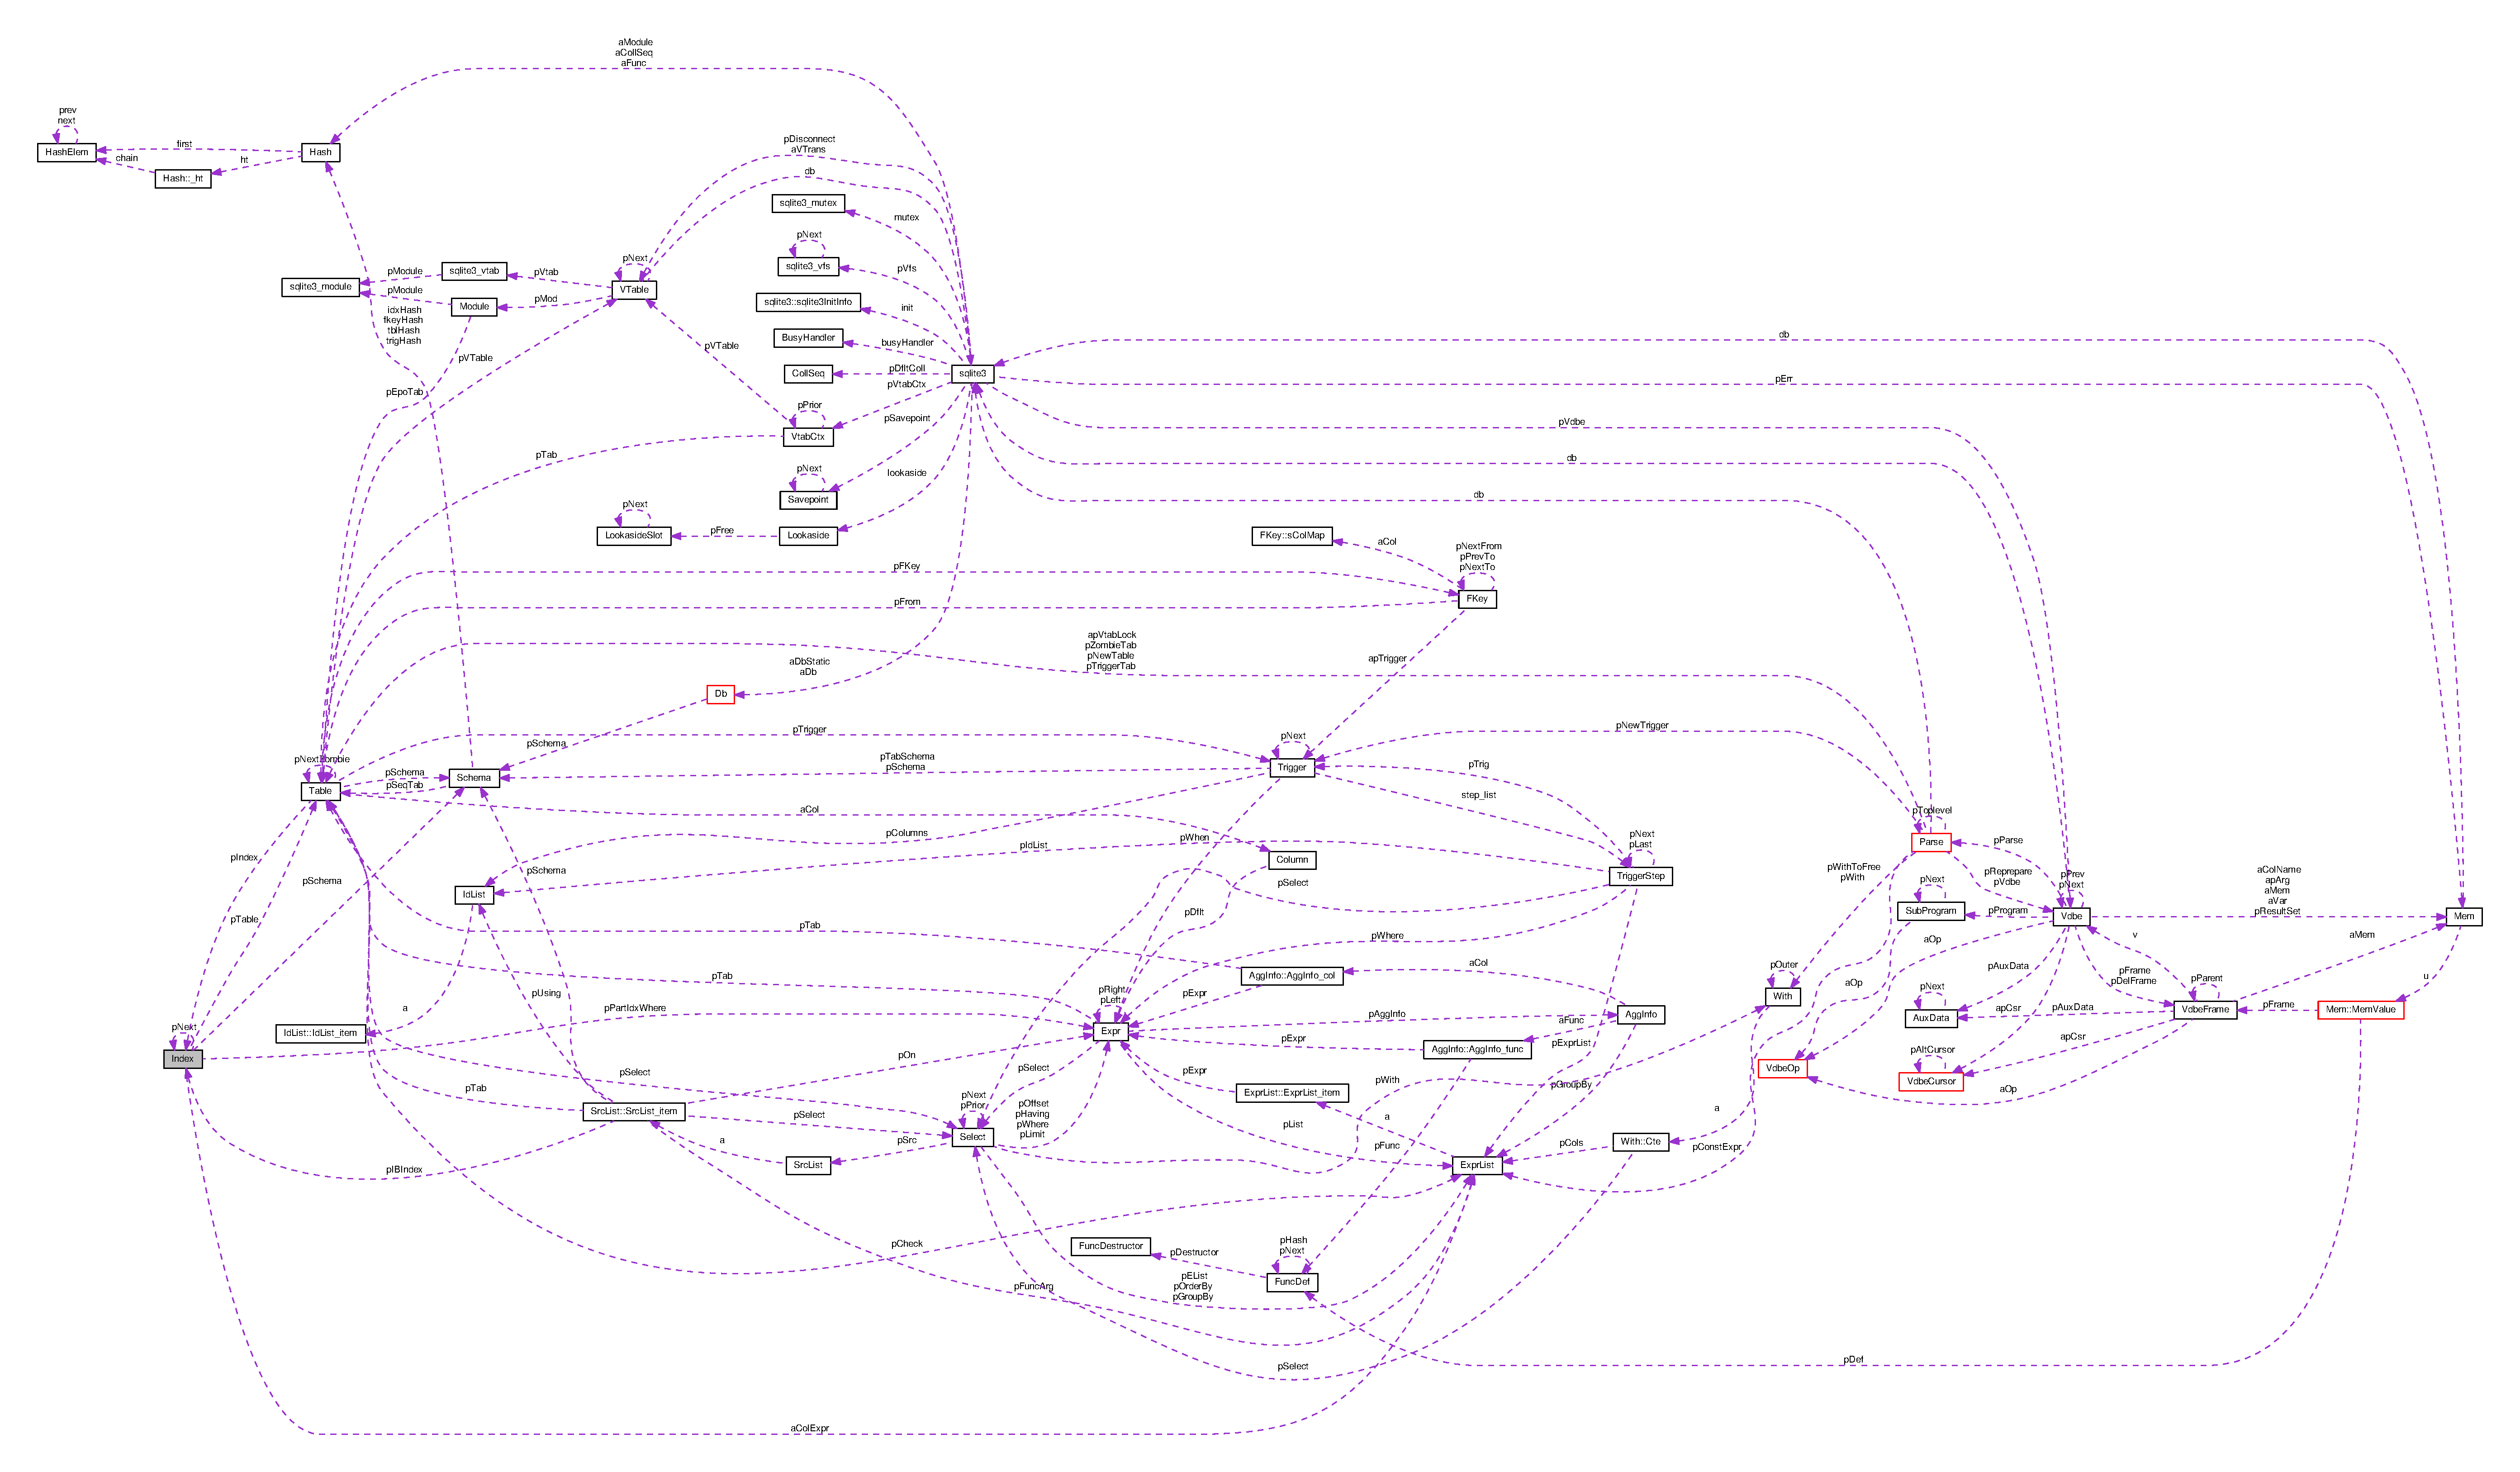
\includegraphics[width=350pt]{structIndex__coll__graph}
\end{center}
\end{figure}
\subsection*{Public Attributes}
\begin{DoxyCompactItemize}
\item 
char $\ast$ {\bfseries z\+Name}\hypertarget{structIndex_a8848cddf6e09f22e3b794ec019082ced}{}\label{structIndex_a8848cddf6e09f22e3b794ec019082ced}

\item 
i16 $\ast$ {\bfseries ai\+Column}\hypertarget{structIndex_a62b5bf88f7c567f15e9a8c9da579d45c}{}\label{structIndex_a62b5bf88f7c567f15e9a8c9da579d45c}

\item 
Log\+Est $\ast$ {\bfseries ai\+Row\+Log\+Est}\hypertarget{structIndex_a830ea536e93022501262afe908bdd35c}{}\label{structIndex_a830ea536e93022501262afe908bdd35c}

\item 
\hyperlink{structTable}{Table} $\ast$ {\bfseries p\+Table}\hypertarget{structIndex_a01c6d4da27cba325ca58f333f87a6f44}{}\label{structIndex_a01c6d4da27cba325ca58f333f87a6f44}

\item 
char $\ast$ {\bfseries z\+Col\+Aff}\hypertarget{structIndex_af076df9f74dd836001c0a59d27274c0e}{}\label{structIndex_af076df9f74dd836001c0a59d27274c0e}

\item 
\hyperlink{structIndex}{Index} $\ast$ {\bfseries p\+Next}\hypertarget{structIndex_a115a17d236bd277d59dd5ea030954c3e}{}\label{structIndex_a115a17d236bd277d59dd5ea030954c3e}

\item 
\hyperlink{structSchema}{Schema} $\ast$ {\bfseries p\+Schema}\hypertarget{structIndex_af14f5ddd57eab2aba63dcb5db2aa92af}{}\label{structIndex_af14f5ddd57eab2aba63dcb5db2aa92af}

\item 
u8 $\ast$ {\bfseries a\+Sort\+Order}\hypertarget{structIndex_a0a3fc87b53193995f59c9657443e9a99}{}\label{structIndex_a0a3fc87b53193995f59c9657443e9a99}

\item 
const char $\ast$$\ast$ {\bfseries az\+Coll}\hypertarget{structIndex_a04f01be3e98aabc4a0516a2fbf28fae1}{}\label{structIndex_a04f01be3e98aabc4a0516a2fbf28fae1}

\item 
\hyperlink{structExpr}{Expr} $\ast$ {\bfseries p\+Part\+Idx\+Where}\hypertarget{structIndex_a92dd15cc702e261dc2face5a27820e07}{}\label{structIndex_a92dd15cc702e261dc2face5a27820e07}

\item 
\hyperlink{structExprList}{Expr\+List} $\ast$ {\bfseries a\+Col\+Expr}\hypertarget{structIndex_ad56e9619762ce33f1a9cd96affc0d3d4}{}\label{structIndex_ad56e9619762ce33f1a9cd96affc0d3d4}

\item 
int {\bfseries tnum}\hypertarget{structIndex_af895a09c01701021c3e36362c04a1ae6}{}\label{structIndex_af895a09c01701021c3e36362c04a1ae6}

\item 
Log\+Est {\bfseries sz\+Idx\+Row}\hypertarget{structIndex_a9048746be17e02ffb3ac6d6a228e4a62}{}\label{structIndex_a9048746be17e02ffb3ac6d6a228e4a62}

\item 
u16 {\bfseries n\+Key\+Col}\hypertarget{structIndex_acfd52a6b0c7be163dcaf524574f69331}{}\label{structIndex_acfd52a6b0c7be163dcaf524574f69331}

\item 
u16 {\bfseries n\+Column}\hypertarget{structIndex_ab0e748636131297b5243e61ee9a8042c}{}\label{structIndex_ab0e748636131297b5243e61ee9a8042c}

\item 
u8 {\bfseries on\+Error}\hypertarget{structIndex_ae8bf87d0414e5c46b86192cfbdd271a7}{}\label{structIndex_ae8bf87d0414e5c46b86192cfbdd271a7}

\item 
unsigned {\bfseries idx\+Type}\+:2\hypertarget{structIndex_aebd62422c514bd90aab41606bec71032}{}\label{structIndex_aebd62422c514bd90aab41606bec71032}

\item 
unsigned {\bfseries b\+Unordered}\+:1\hypertarget{structIndex_ae96b00c29b348bce9d58a5073fdb6d3e}{}\label{structIndex_ae96b00c29b348bce9d58a5073fdb6d3e}

\item 
unsigned {\bfseries uniq\+Not\+Null}\+:1\hypertarget{structIndex_a541590f6cf6c45705b3ef19fdce091ca}{}\label{structIndex_a541590f6cf6c45705b3ef19fdce091ca}

\item 
unsigned {\bfseries is\+Resized}\+:1\hypertarget{structIndex_ad9c4a83513b3cf885782dcd459ed061f}{}\label{structIndex_ad9c4a83513b3cf885782dcd459ed061f}

\item 
unsigned {\bfseries is\+Covering}\+:1\hypertarget{structIndex_ac4151fa2557d26d7c538f25a03d0b44e}{}\label{structIndex_ac4151fa2557d26d7c538f25a03d0b44e}

\item 
unsigned {\bfseries no\+Skip\+Scan}\+:1\hypertarget{structIndex_a7704321883c8b38e6dcca88b5886d4ee}{}\label{structIndex_a7704321883c8b38e6dcca88b5886d4ee}

\end{DoxyCompactItemize}


The documentation for this struct was generated from the following file\+:\begin{DoxyCompactItemize}
\item 
sqlite3.\+c\end{DoxyCompactItemize}

\hypertarget{structIndexSample}{}\section{Index\+Sample Struct Reference}
\label{structIndexSample}\index{Index\+Sample@{Index\+Sample}}
\subsection*{Public Attributes}
\begin{DoxyCompactItemize}
\item 
void $\ast$ {\bfseries p}\hypertarget{structIndexSample_a539f00d3096fd379146e77e74b513dac}{}\label{structIndexSample_a539f00d3096fd379146e77e74b513dac}

\item 
int {\bfseries n}\hypertarget{structIndexSample_a89016f3b6580ee9c63c4ac78e2e6e76c}{}\label{structIndexSample_a89016f3b6580ee9c63c4ac78e2e6e76c}

\item 
t\+Rowcnt $\ast$ {\bfseries an\+Eq}\hypertarget{structIndexSample_a048e60e638c6e0305812102366822e67}{}\label{structIndexSample_a048e60e638c6e0305812102366822e67}

\item 
t\+Rowcnt $\ast$ {\bfseries an\+Lt}\hypertarget{structIndexSample_a4853d16cdb7cf5099e8478471ae729de}{}\label{structIndexSample_a4853d16cdb7cf5099e8478471ae729de}

\item 
t\+Rowcnt $\ast$ {\bfseries an\+D\+Lt}\hypertarget{structIndexSample_ab17baab68e2890d9939c3840987051c2}{}\label{structIndexSample_ab17baab68e2890d9939c3840987051c2}

\end{DoxyCompactItemize}


The documentation for this struct was generated from the following file\+:\begin{DoxyCompactItemize}
\item 
sqlite3.\+c\end{DoxyCompactItemize}

\hypertarget{structInitData}{}\section{Init\+Data Struct Reference}
\label{structInitData}\index{Init\+Data@{Init\+Data}}


Collaboration diagram for Init\+Data\+:
% FIG 0
\subsection*{Public Attributes}
\begin{DoxyCompactItemize}
\item 
\hyperlink{structsqlite3}{sqlite3} $\ast$ {\bfseries db}\hypertarget{structInitData_adc9e29c56e0392076e92d7f4b29fa272}{}\label{structInitData_adc9e29c56e0392076e92d7f4b29fa272}

\item 
char $\ast$$\ast$ {\bfseries pz\+Err\+Msg}\hypertarget{structInitData_aa8aef34241ec214f038b38932ffe1357}{}\label{structInitData_aa8aef34241ec214f038b38932ffe1357}

\item 
int {\bfseries i\+Db}\hypertarget{structInitData_ad6c7953b49d351cd9fb14e3394010689}{}\label{structInitData_ad6c7953b49d351cd9fb14e3394010689}

\item 
int {\bfseries rc}\hypertarget{structInitData_a627153a3de2c4d159ae44ebc03961592}{}\label{structInitData_a627153a3de2c4d159ae44ebc03961592}

\end{DoxyCompactItemize}


The documentation for this struct was generated from the following file\+:\begin{DoxyCompactItemize}
\item 
sqlite3.\+c\end{DoxyCompactItemize}

\hypertarget{structIntegrityCk}{}\section{Integrity\+Ck Struct Reference}
\label{structIntegrityCk}\index{Integrity\+Ck@{Integrity\+Ck}}


Collaboration diagram for Integrity\+Ck\+:\nopagebreak
\begin{figure}[H]
\begin{center}
\leavevmode
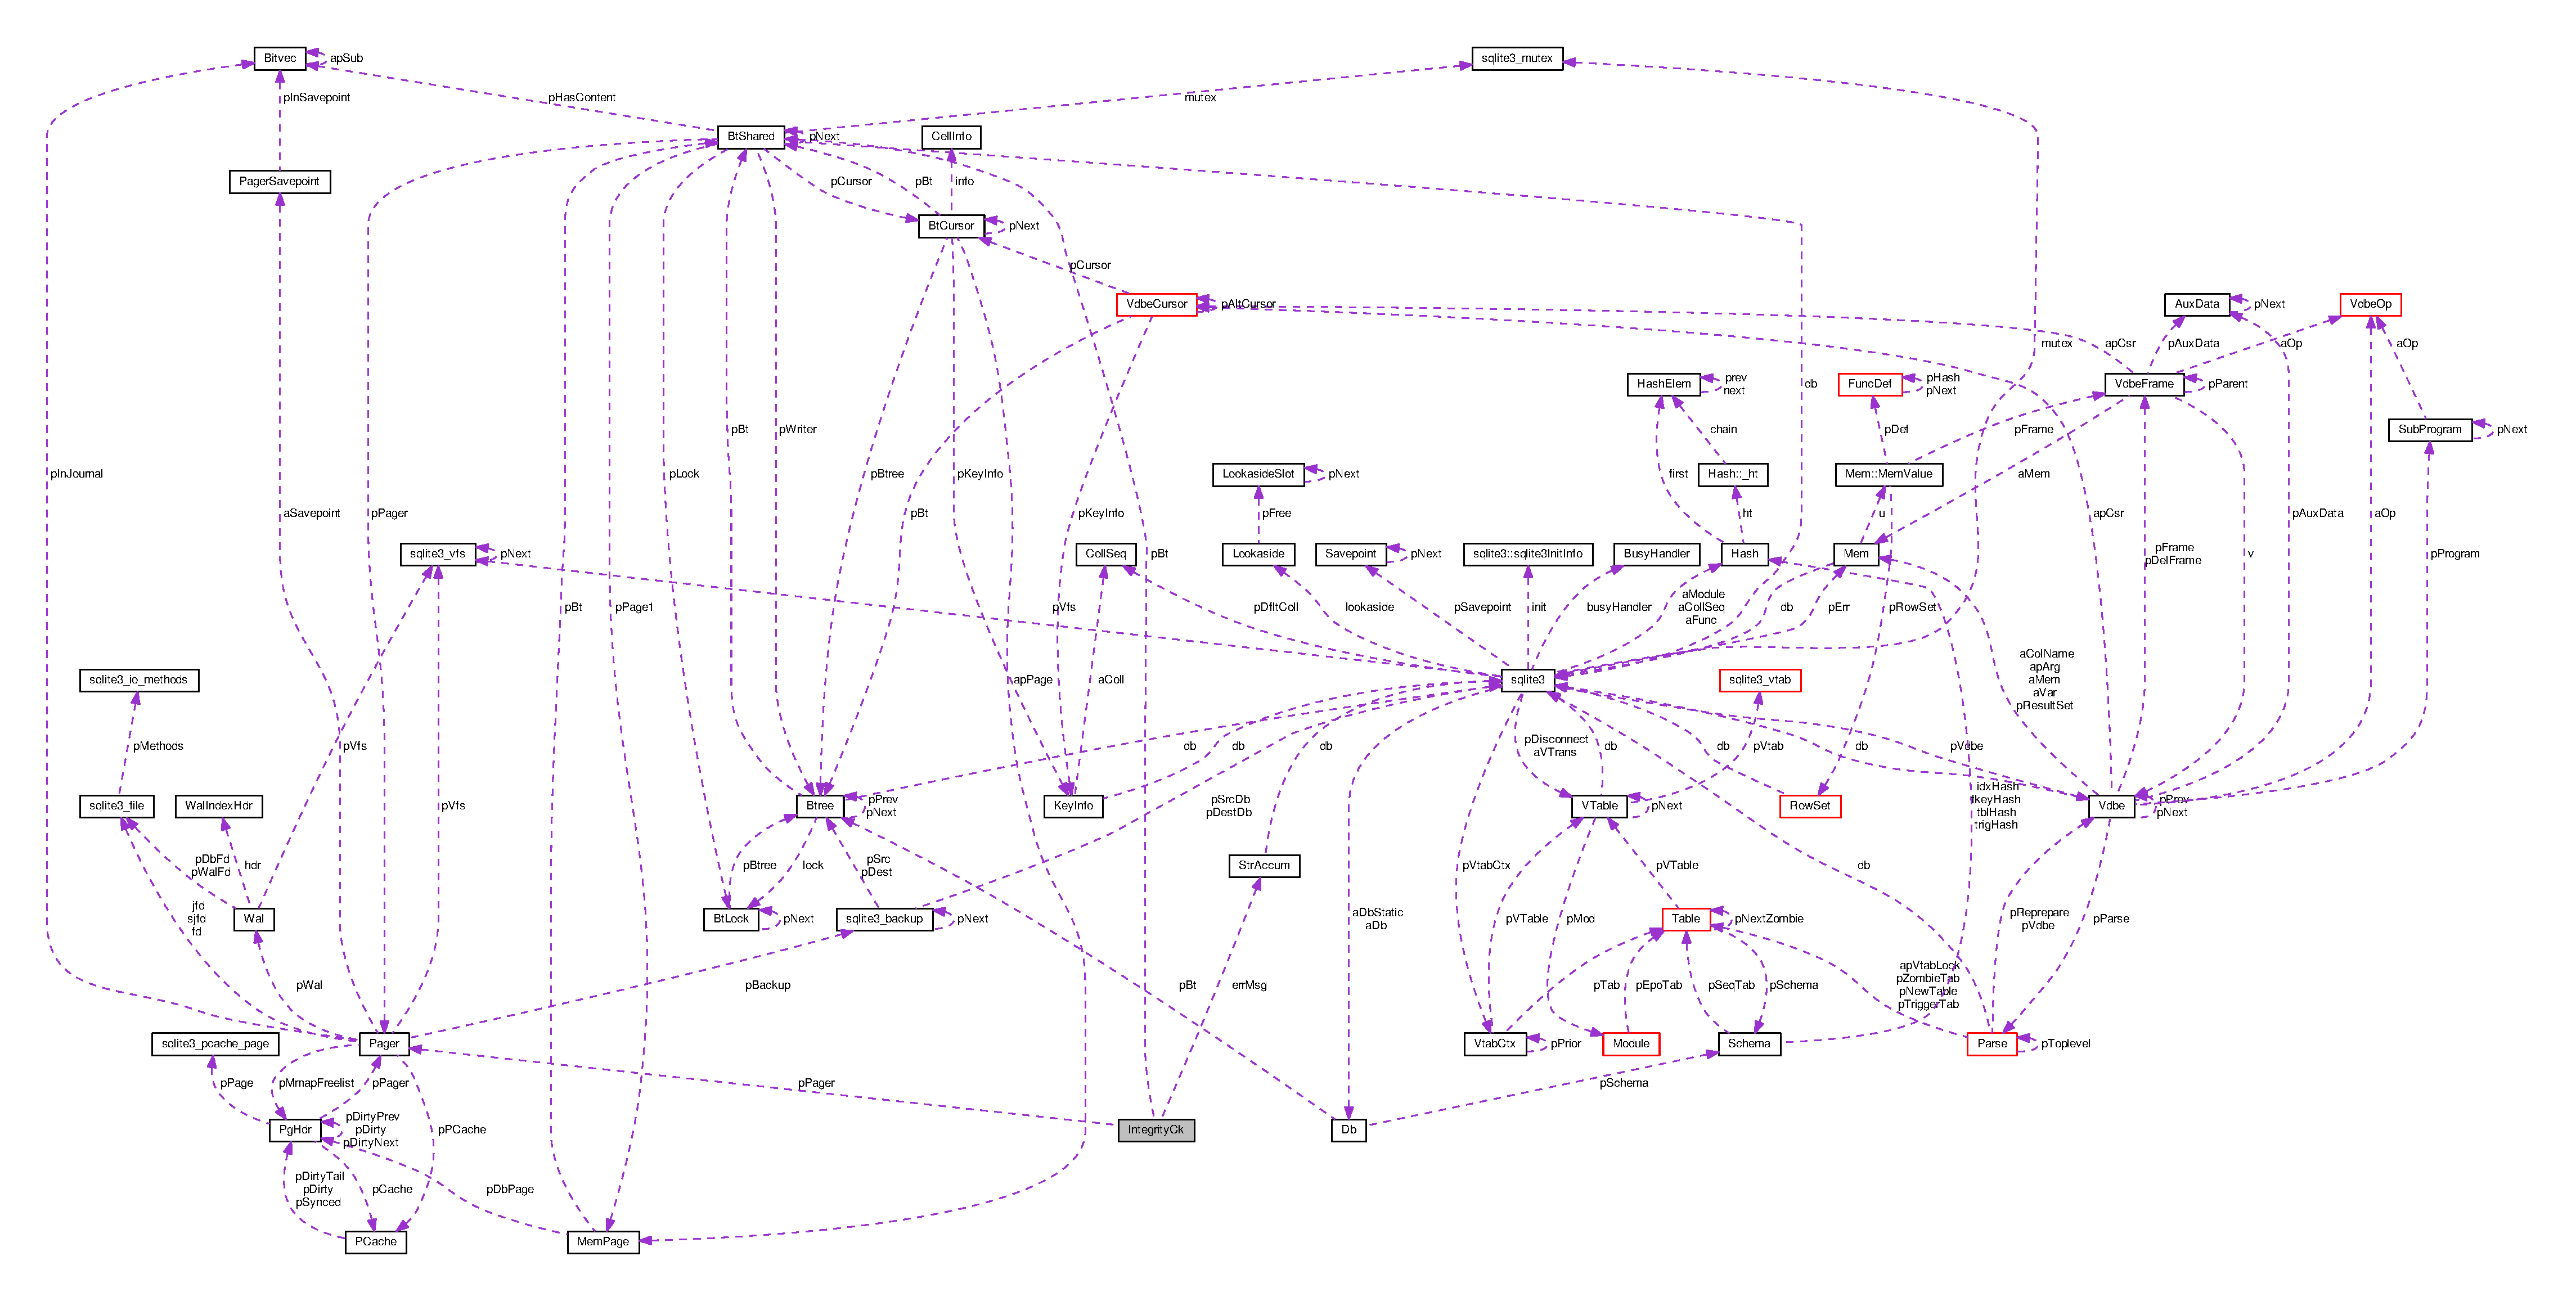
\includegraphics[width=350pt]{structIntegrityCk__coll__graph}
\end{center}
\end{figure}
\subsection*{Public Attributes}
\begin{DoxyCompactItemize}
\item 
\hyperlink{structBtShared}{Bt\+Shared} $\ast$ {\bfseries p\+Bt}\hypertarget{structIntegrityCk_a65f03f54514f504bd871bb2ccd3da188}{}\label{structIntegrityCk_a65f03f54514f504bd871bb2ccd3da188}

\item 
\hyperlink{structPager}{Pager} $\ast$ {\bfseries p\+Pager}\hypertarget{structIntegrityCk_a87e7f8b012b61b61fae359269cbacce4}{}\label{structIntegrityCk_a87e7f8b012b61b61fae359269cbacce4}

\item 
u8 $\ast$ {\bfseries a\+Pg\+Ref}\hypertarget{structIntegrityCk_a317f80aef5842ad69df75b55e14118d1}{}\label{structIntegrityCk_a317f80aef5842ad69df75b55e14118d1}

\item 
Pgno {\bfseries n\+Page}\hypertarget{structIntegrityCk_a04f496ef7239aea6dccb6a861bb5a798}{}\label{structIntegrityCk_a04f496ef7239aea6dccb6a861bb5a798}

\item 
int {\bfseries mx\+Err}\hypertarget{structIntegrityCk_a9daa97cdcb1366c503451ab2af9e7ba6}{}\label{structIntegrityCk_a9daa97cdcb1366c503451ab2af9e7ba6}

\item 
int {\bfseries n\+Err}\hypertarget{structIntegrityCk_a52c815a1d19be87d0ab4dc0a4e4d38e2}{}\label{structIntegrityCk_a52c815a1d19be87d0ab4dc0a4e4d38e2}

\item 
int {\bfseries malloc\+Failed}\hypertarget{structIntegrityCk_a8e448c1d6483a0326a7ec39291782030}{}\label{structIntegrityCk_a8e448c1d6483a0326a7ec39291782030}

\item 
const char $\ast$ {\bfseries z\+Pfx}\hypertarget{structIntegrityCk_a126e42d437777815b1c1d74bcacb3b38}{}\label{structIntegrityCk_a126e42d437777815b1c1d74bcacb3b38}

\item 
int {\bfseries v1}\hypertarget{structIntegrityCk_a94edb493175bd0c1862efbaeaff63be3}{}\label{structIntegrityCk_a94edb493175bd0c1862efbaeaff63be3}

\item 
int {\bfseries v2}\hypertarget{structIntegrityCk_a0dd13b39fb4fd4e42de8ebf05af5c287}{}\label{structIntegrityCk_a0dd13b39fb4fd4e42de8ebf05af5c287}

\item 
\hyperlink{structStrAccum}{Str\+Accum} {\bfseries err\+Msg}\hypertarget{structIntegrityCk_a1e9b79bb1d7b22a840001333200a950e}{}\label{structIntegrityCk_a1e9b79bb1d7b22a840001333200a950e}

\item 
u32 $\ast$ {\bfseries heap}\hypertarget{structIntegrityCk_aada31529ac9fd90643f22cbb79cd916a}{}\label{structIntegrityCk_aada31529ac9fd90643f22cbb79cd916a}

\end{DoxyCompactItemize}


The documentation for this struct was generated from the following file\+:\begin{DoxyCompactItemize}
\item 
sqlite3.\+c\end{DoxyCompactItemize}

\hypertarget{structKeyInfo}{}\section{Key\+Info Struct Reference}
\label{structKeyInfo}\index{Key\+Info@{Key\+Info}}


Collaboration diagram for Key\+Info\+:
% FIG 0
\subsection*{Public Attributes}
\begin{DoxyCompactItemize}
\item 
u32 {\bfseries n\+Ref}\hypertarget{structKeyInfo_a4f6162c8d1ecc9e3c7471571e8918972}{}\label{structKeyInfo_a4f6162c8d1ecc9e3c7471571e8918972}

\item 
u8 {\bfseries enc}\hypertarget{structKeyInfo_a37972825f9a148668e979be12465e832}{}\label{structKeyInfo_a37972825f9a148668e979be12465e832}

\item 
u16 {\bfseries n\+Field}\hypertarget{structKeyInfo_af70436487a95e445d540bfc4ca1d3f0b}{}\label{structKeyInfo_af70436487a95e445d540bfc4ca1d3f0b}

\item 
u16 {\bfseries n\+X\+Field}\hypertarget{structKeyInfo_ac77a6b68f879a69127a8797b62a2f3aa}{}\label{structKeyInfo_ac77a6b68f879a69127a8797b62a2f3aa}

\item 
\hyperlink{structsqlite3}{sqlite3} $\ast$ {\bfseries db}\hypertarget{structKeyInfo_af2e7a3a411f5ca1ccf6de77d320b59db}{}\label{structKeyInfo_af2e7a3a411f5ca1ccf6de77d320b59db}

\item 
u8 $\ast$ {\bfseries a\+Sort\+Order}\hypertarget{structKeyInfo_ac5fe4bd0172a1f11f41f678528a7b21e}{}\label{structKeyInfo_ac5fe4bd0172a1f11f41f678528a7b21e}

\item 
\hyperlink{structCollSeq}{Coll\+Seq} $\ast$ {\bfseries a\+Coll} \mbox{[}1\mbox{]}\hypertarget{structKeyInfo_ad43aa024fca5a065e75d8e24b231adcb}{}\label{structKeyInfo_ad43aa024fca5a065e75d8e24b231adcb}

\end{DoxyCompactItemize}


The documentation for this struct was generated from the following file\+:\begin{DoxyCompactItemize}
\item 
sqlite3.\+c\end{DoxyCompactItemize}

\hypertarget{structLimitVal}{}\section{Limit\+Val Struct Reference}
\label{structLimitVal}\index{Limit\+Val@{Limit\+Val}}


Collaboration diagram for Limit\+Val\+:
% FIG 0
\subsection*{Public Attributes}
\begin{DoxyCompactItemize}
\item 
\hyperlink{structExpr}{Expr} $\ast$ {\bfseries p\+Limit}\hypertarget{structLimitVal_a96094d1b395a3f455263ff5907d72ed6}{}\label{structLimitVal_a96094d1b395a3f455263ff5907d72ed6}

\item 
\hyperlink{structExpr}{Expr} $\ast$ {\bfseries p\+Offset}\hypertarget{structLimitVal_a43dedf453a8e5cb8091fcde524a7c736}{}\label{structLimitVal_a43dedf453a8e5cb8091fcde524a7c736}

\end{DoxyCompactItemize}


The documentation for this struct was generated from the following file\+:\begin{DoxyCompactItemize}
\item 
sqlite3.\+c\end{DoxyCompactItemize}

\hypertarget{structLookaside}{}\section{Lookaside Struct Reference}
\label{structLookaside}\index{Lookaside@{Lookaside}}


Collaboration diagram for Lookaside\+:\nopagebreak
\begin{figure}[H]
\begin{center}
\leavevmode
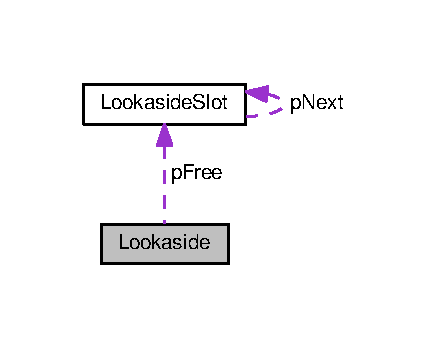
\includegraphics[width=206pt]{structLookaside__coll__graph}
\end{center}
\end{figure}
\subsection*{Public Attributes}
\begin{DoxyCompactItemize}
\item 
u32 {\bfseries b\+Disable}\hypertarget{structLookaside_ac81ee3b5b12d0bc89ed1286718224db1}{}\label{structLookaside_ac81ee3b5b12d0bc89ed1286718224db1}

\item 
u16 {\bfseries sz}\hypertarget{structLookaside_a2e8346b6cebbb64d9a6886a19ef843a1}{}\label{structLookaside_a2e8346b6cebbb64d9a6886a19ef843a1}

\item 
u8 {\bfseries b\+Malloced}\hypertarget{structLookaside_a218f14cf9eb2c430867d286e9ac57ac5}{}\label{structLookaside_a218f14cf9eb2c430867d286e9ac57ac5}

\item 
int {\bfseries n\+Out}\hypertarget{structLookaside_a4cdd49fa554f877928d5bb31d55b32e9}{}\label{structLookaside_a4cdd49fa554f877928d5bb31d55b32e9}

\item 
int {\bfseries mx\+Out}\hypertarget{structLookaside_a2ce364d95b55913df986999de442e4f9}{}\label{structLookaside_a2ce364d95b55913df986999de442e4f9}

\item 
int {\bfseries an\+Stat} \mbox{[}3\mbox{]}\hypertarget{structLookaside_a7d875204cb05a327bb1652139faa4374}{}\label{structLookaside_a7d875204cb05a327bb1652139faa4374}

\item 
\hyperlink{structLookasideSlot}{Lookaside\+Slot} $\ast$ {\bfseries p\+Free}\hypertarget{structLookaside_a318d2faa7f976f9d1b3c6e08bdc1d992}{}\label{structLookaside_a318d2faa7f976f9d1b3c6e08bdc1d992}

\item 
void $\ast$ {\bfseries p\+Start}\hypertarget{structLookaside_a47073fcdffdc5a7a1464f0d09bfc17f9}{}\label{structLookaside_a47073fcdffdc5a7a1464f0d09bfc17f9}

\item 
void $\ast$ {\bfseries p\+End}\hypertarget{structLookaside_ad3555c5558e104f2b82f62bf642cf831}{}\label{structLookaside_ad3555c5558e104f2b82f62bf642cf831}

\end{DoxyCompactItemize}


The documentation for this struct was generated from the following file\+:\begin{DoxyCompactItemize}
\item 
sqlite3.\+c\end{DoxyCompactItemize}

\hypertarget{structLookasideSlot}{}\section{Lookaside\+Slot Struct Reference}
\label{structLookasideSlot}\index{Lookaside\+Slot@{Lookaside\+Slot}}


Collaboration diagram for Lookaside\+Slot\+:
% FIG 0
\subsection*{Public Attributes}
\begin{DoxyCompactItemize}
\item 
\hyperlink{structLookasideSlot}{Lookaside\+Slot} $\ast$ {\bfseries p\+Next}\hypertarget{structLookasideSlot_a3c3dd4a770ded51a68e8a651eba40f66}{}\label{structLookasideSlot_a3c3dd4a770ded51a68e8a651eba40f66}

\end{DoxyCompactItemize}


The documentation for this struct was generated from the following file\+:\begin{DoxyCompactItemize}
\item 
sqlite3.\+c\end{DoxyCompactItemize}

\hypertarget{structMem}{}\section{Mem Struct Reference}
\label{structMem}\index{Mem@{Mem}}


Collaboration diagram for Mem\+:\nopagebreak
\begin{figure}[H]
\begin{center}
\leavevmode
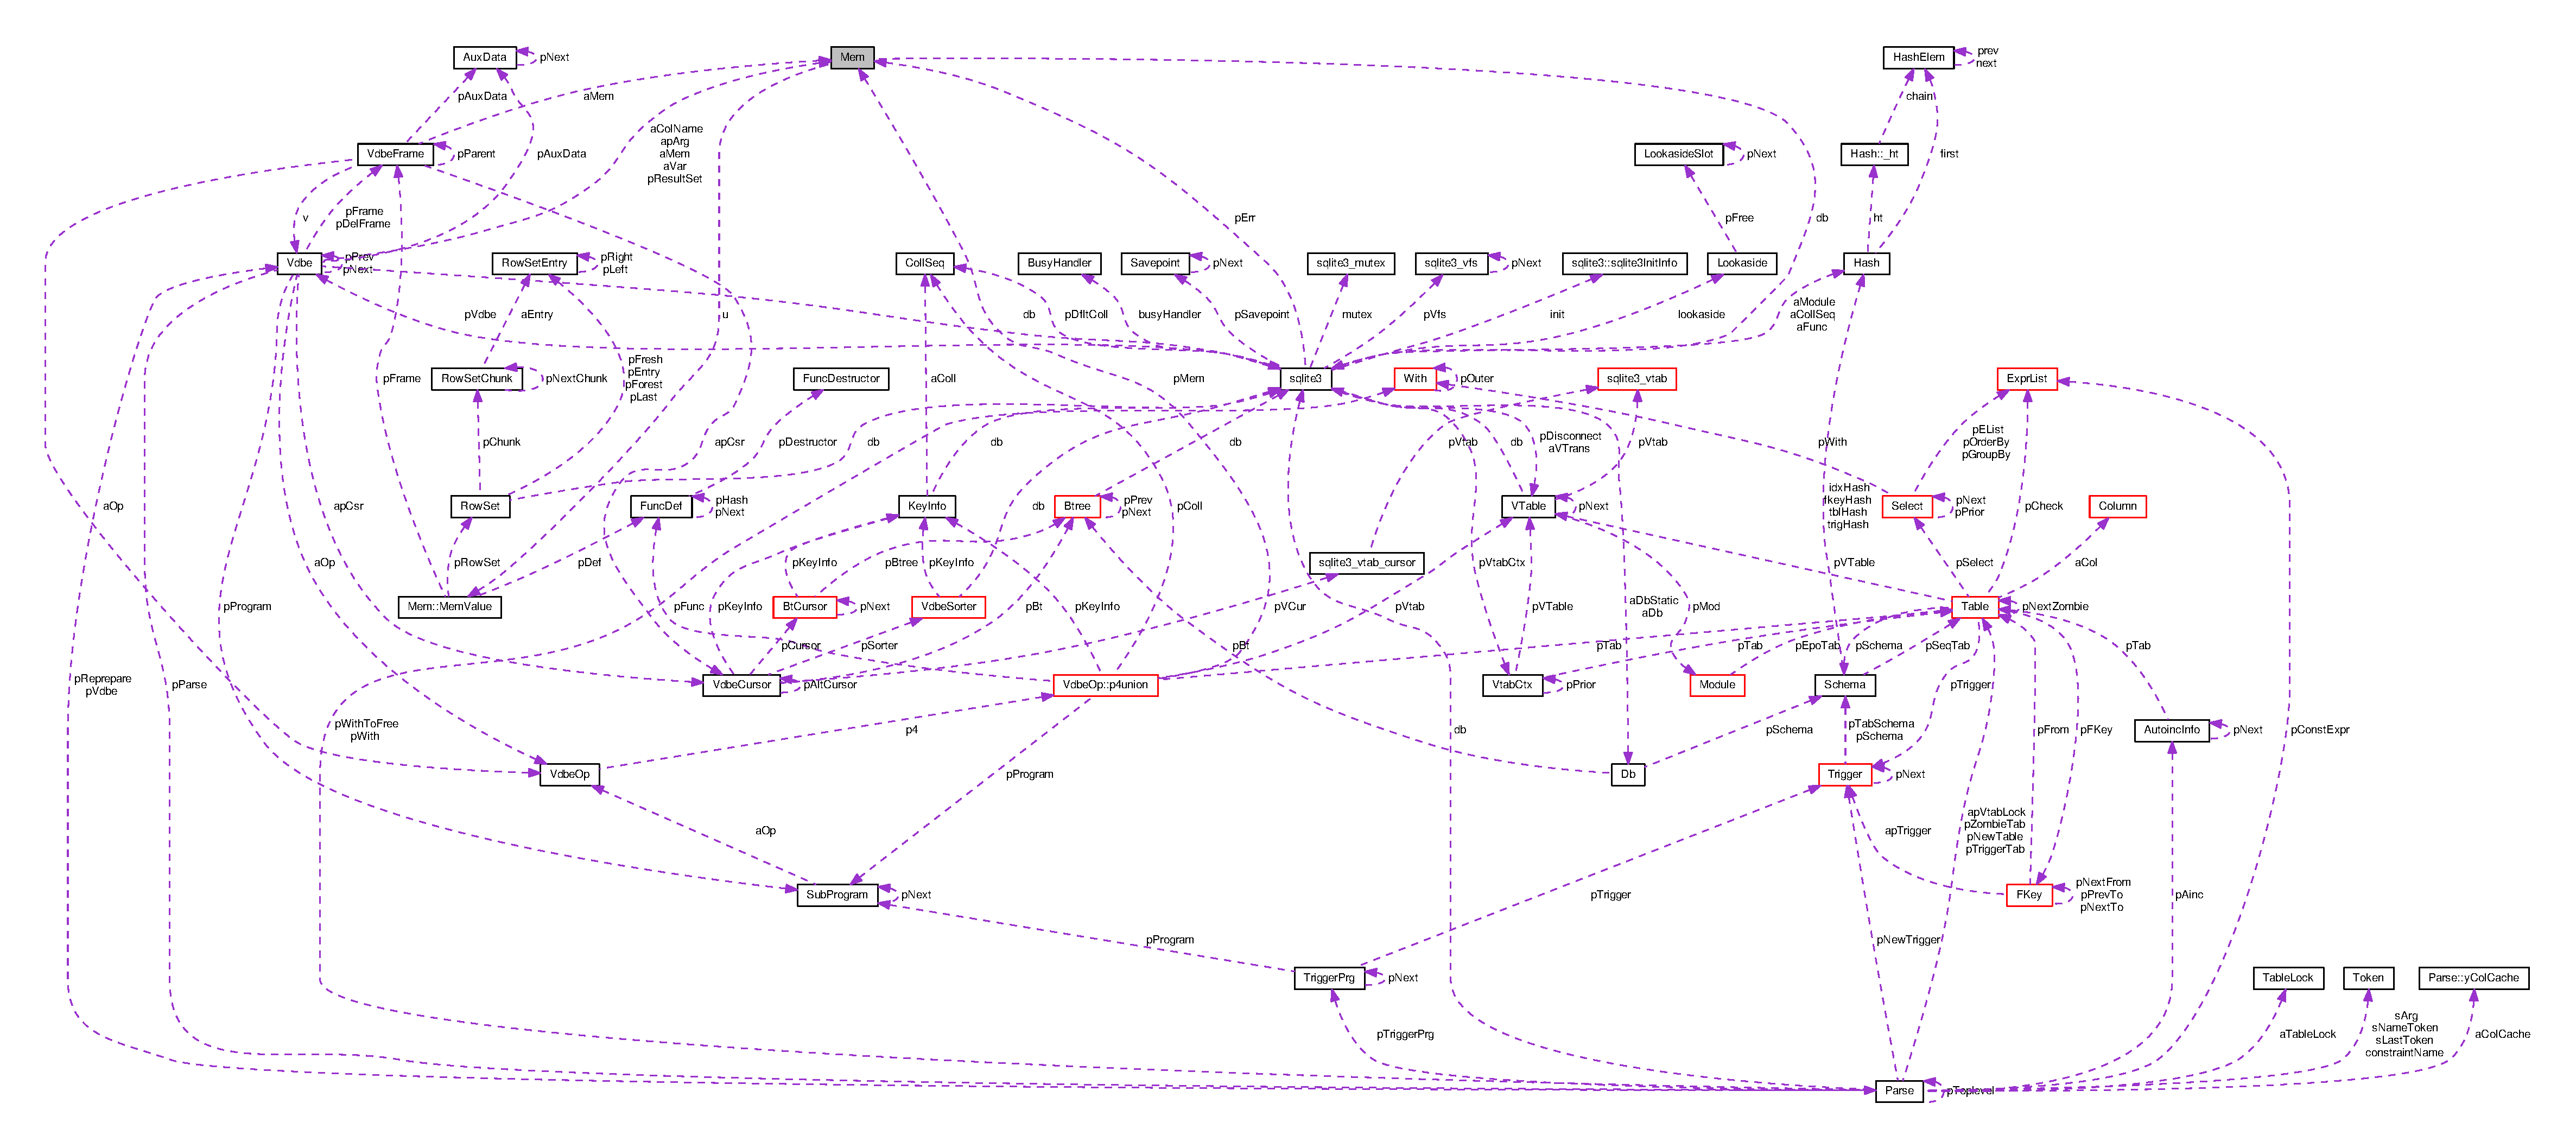
\includegraphics[width=350pt]{structMem__coll__graph}
\end{center}
\end{figure}
\subsection*{Classes}
\begin{DoxyCompactItemize}
\item 
union \hyperlink{unionMem_1_1MemValue}{Mem\+Value}
\end{DoxyCompactItemize}
\subsection*{Public Attributes}
\begin{DoxyCompactItemize}
\item 
union \hyperlink{unionMem_1_1MemValue}{Mem\+::\+Mem\+Value} {\bfseries u}\hypertarget{structMem_ac280628b51c0d03433ce3a05821b2911}{}\label{structMem_ac280628b51c0d03433ce3a05821b2911}

\item 
u16 {\bfseries flags}\hypertarget{structMem_a209bf3317161d1e33af9fe8b512f4974}{}\label{structMem_a209bf3317161d1e33af9fe8b512f4974}

\item 
u8 {\bfseries enc}\hypertarget{structMem_af437c99e92b8e729b70f82fa94e96bff}{}\label{structMem_af437c99e92b8e729b70f82fa94e96bff}

\item 
u8 {\bfseries e\+Subtype}\hypertarget{structMem_acb9ea95c050b4a96bd4c41386b05342a}{}\label{structMem_acb9ea95c050b4a96bd4c41386b05342a}

\item 
int {\bfseries n}\hypertarget{structMem_a5a613756e096c221ec68077c28424d84}{}\label{structMem_a5a613756e096c221ec68077c28424d84}

\item 
char $\ast$ {\bfseries z}\hypertarget{structMem_a85c51a0b445063ba913693517860f5ea}{}\label{structMem_a85c51a0b445063ba913693517860f5ea}

\item 
char $\ast$ {\bfseries z\+Malloc}\hypertarget{structMem_a68cd8f196d9dc8ab27845e1b4abbc95c}{}\label{structMem_a68cd8f196d9dc8ab27845e1b4abbc95c}

\item 
int {\bfseries sz\+Malloc}\hypertarget{structMem_a857df48ae7c5d3af4a8a8a3ed95bc873}{}\label{structMem_a857df48ae7c5d3af4a8a8a3ed95bc873}

\item 
u32 {\bfseries u\+Temp}\hypertarget{structMem_a36fce871381c6e796488034e41388a83}{}\label{structMem_a36fce871381c6e796488034e41388a83}

\item 
\hyperlink{structsqlite3}{sqlite3} $\ast$ {\bfseries db}\hypertarget{structMem_a478da33d1e83a23931b372f9ddc706f2}{}\label{structMem_a478da33d1e83a23931b372f9ddc706f2}

\item 
void($\ast$ {\bfseries x\+Del} )(void $\ast$)\hypertarget{structMem_a0d89e070132d482e8f3da755f0bb17bb}{}\label{structMem_a0d89e070132d482e8f3da755f0bb17bb}

\end{DoxyCompactItemize}


The documentation for this struct was generated from the following file\+:\begin{DoxyCompactItemize}
\item 
sqlite3.\+c\end{DoxyCompactItemize}

\hypertarget{structMemJournal}{}\section{Mem\+Journal Struct Reference}
\label{structMemJournal}\index{Mem\+Journal@{Mem\+Journal}}


Collaboration diagram for Mem\+Journal\+:\nopagebreak
\begin{figure}[H]
\begin{center}
\leavevmode
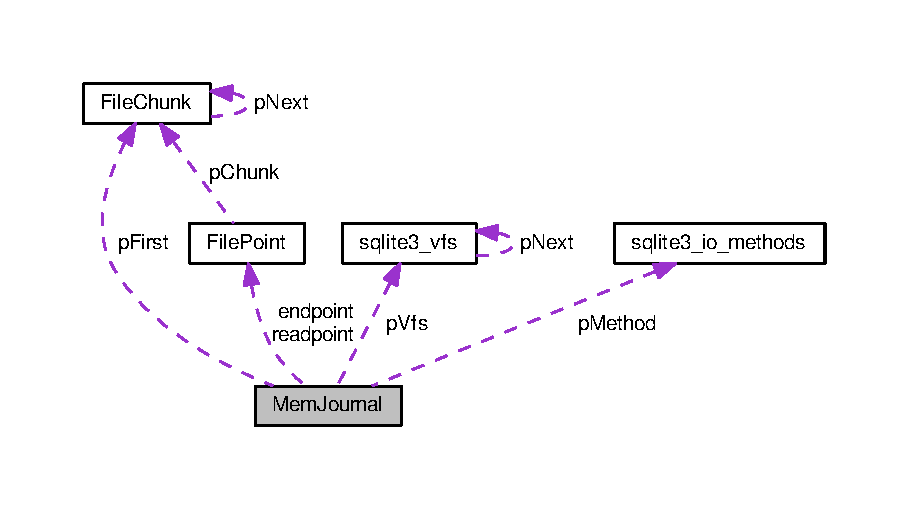
\includegraphics[width=350pt]{structMemJournal__coll__graph}
\end{center}
\end{figure}
\subsection*{Public Attributes}
\begin{DoxyCompactItemize}
\item 
const \hyperlink{structsqlite3__io__methods}{sqlite3\+\_\+io\+\_\+methods} $\ast$ {\bfseries p\+Method}\hypertarget{structMemJournal_aad04f16d7faaeb548b3197cce7b0d37f}{}\label{structMemJournal_aad04f16d7faaeb548b3197cce7b0d37f}

\item 
int {\bfseries n\+Chunk\+Size}\hypertarget{structMemJournal_a15ba0375c0a30b355f5f7594e8804c1a}{}\label{structMemJournal_a15ba0375c0a30b355f5f7594e8804c1a}

\item 
int {\bfseries n\+Spill}\hypertarget{structMemJournal_afee076918f23dc1cd05681cb0504a77d}{}\label{structMemJournal_afee076918f23dc1cd05681cb0504a77d}

\item 
int {\bfseries n\+Size}\hypertarget{structMemJournal_a5c3de9e25d0e0a6fb36beec447de0c36}{}\label{structMemJournal_a5c3de9e25d0e0a6fb36beec447de0c36}

\item 
\hyperlink{structFileChunk}{File\+Chunk} $\ast$ {\bfseries p\+First}\hypertarget{structMemJournal_ade7a6dea7b38a8a86f33476ae207765f}{}\label{structMemJournal_ade7a6dea7b38a8a86f33476ae207765f}

\item 
\hyperlink{structFilePoint}{File\+Point} {\bfseries endpoint}\hypertarget{structMemJournal_ac69637f95cfbce175cbeef00f71e59a9}{}\label{structMemJournal_ac69637f95cfbce175cbeef00f71e59a9}

\item 
\hyperlink{structFilePoint}{File\+Point} {\bfseries readpoint}\hypertarget{structMemJournal_a5645d38e1a488b62b5f63112628bf472}{}\label{structMemJournal_a5645d38e1a488b62b5f63112628bf472}

\item 
int {\bfseries flags}\hypertarget{structMemJournal_a1fcfbcbb9da77a5cefef038b1b846f35}{}\label{structMemJournal_a1fcfbcbb9da77a5cefef038b1b846f35}

\item 
\hyperlink{structsqlite3__vfs}{sqlite3\+\_\+vfs} $\ast$ {\bfseries p\+Vfs}\hypertarget{structMemJournal_a5174aefb3d641db787fd1952e6e2fd7d}{}\label{structMemJournal_a5174aefb3d641db787fd1952e6e2fd7d}

\item 
const char $\ast$ {\bfseries z\+Journal}\hypertarget{structMemJournal_a60e0eed44abd876329d1f7d9a4c0d773}{}\label{structMemJournal_a60e0eed44abd876329d1f7d9a4c0d773}

\end{DoxyCompactItemize}


The documentation for this struct was generated from the following file\+:\begin{DoxyCompactItemize}
\item 
sqlite3.\+c\end{DoxyCompactItemize}

\hypertarget{structMemPage}{}\section{Mem\+Page Struct Reference}
\label{structMemPage}\index{Mem\+Page@{Mem\+Page}}


Collaboration diagram for Mem\+Page\+:
% FIG 0
\subsection*{Public Attributes}
\begin{DoxyCompactItemize}
\item 
u8 {\bfseries is\+Init}\hypertarget{structMemPage_a3ab4ace46245be0fb2fb19eaa2862019}{}\label{structMemPage_a3ab4ace46245be0fb2fb19eaa2862019}

\item 
u8 {\bfseries n\+Overflow}\hypertarget{structMemPage_a3f7fa1a1eba3af840ef887e8ddd6d2cc}{}\label{structMemPage_a3f7fa1a1eba3af840ef887e8ddd6d2cc}

\item 
u8 {\bfseries int\+Key}\hypertarget{structMemPage_a46784c3c4708c7a582cff81a29c55323}{}\label{structMemPage_a46784c3c4708c7a582cff81a29c55323}

\item 
u8 {\bfseries int\+Key\+Leaf}\hypertarget{structMemPage_a7c30c56237c38e0b81842ae2a6bae9d7}{}\label{structMemPage_a7c30c56237c38e0b81842ae2a6bae9d7}

\item 
u8 {\bfseries leaf}\hypertarget{structMemPage_af18504bd0a2e7d39d9b485d434af0447}{}\label{structMemPage_af18504bd0a2e7d39d9b485d434af0447}

\item 
u8 {\bfseries hdr\+Offset}\hypertarget{structMemPage_a01967a1a593980fb71c8ccf3393ae156}{}\label{structMemPage_a01967a1a593980fb71c8ccf3393ae156}

\item 
u8 {\bfseries child\+Ptr\+Size}\hypertarget{structMemPage_aeba10281fc255d9bbc0e31486f8fbd48}{}\label{structMemPage_aeba10281fc255d9bbc0e31486f8fbd48}

\item 
u8 {\bfseries max1byte\+Payload}\hypertarget{structMemPage_a79548547cafb0e6d8549006bdc553f0a}{}\label{structMemPage_a79548547cafb0e6d8549006bdc553f0a}

\item 
u8 {\bfseries b\+Busy}\hypertarget{structMemPage_a0b7935a6fdec1d6d31c4b3952b0461ea}{}\label{structMemPage_a0b7935a6fdec1d6d31c4b3952b0461ea}

\item 
u16 {\bfseries max\+Local}\hypertarget{structMemPage_a36394b7c3abf4652e7a24be4ab314f13}{}\label{structMemPage_a36394b7c3abf4652e7a24be4ab314f13}

\item 
u16 {\bfseries min\+Local}\hypertarget{structMemPage_a95cab31aa57bf8b478be273557c5c807}{}\label{structMemPage_a95cab31aa57bf8b478be273557c5c807}

\item 
u16 {\bfseries cell\+Offset}\hypertarget{structMemPage_a324ed834d93c3ae72994fb5730940521}{}\label{structMemPage_a324ed834d93c3ae72994fb5730940521}

\item 
u16 {\bfseries n\+Free}\hypertarget{structMemPage_a3418a9aee707f57a73d8470f8a1228a8}{}\label{structMemPage_a3418a9aee707f57a73d8470f8a1228a8}

\item 
u16 {\bfseries n\+Cell}\hypertarget{structMemPage_a35d1d8f836201b82b1eb778ce0e324f4}{}\label{structMemPage_a35d1d8f836201b82b1eb778ce0e324f4}

\item 
u16 {\bfseries mask\+Page}\hypertarget{structMemPage_aa3d64e8755cc9f431bbc8423a2b506ec}{}\label{structMemPage_aa3d64e8755cc9f431bbc8423a2b506ec}

\item 
u16 {\bfseries ai\+Ovfl} \mbox{[}5\mbox{]}\hypertarget{structMemPage_a857e00533053fe6017c6e08b1b240661}{}\label{structMemPage_a857e00533053fe6017c6e08b1b240661}

\item 
u8 $\ast$ {\bfseries ap\+Ovfl} \mbox{[}5\mbox{]}\hypertarget{structMemPage_a3a6347d06b1e85938605d9a44f193cb9}{}\label{structMemPage_a3a6347d06b1e85938605d9a44f193cb9}

\item 
\hyperlink{structBtShared}{Bt\+Shared} $\ast$ {\bfseries p\+Bt}\hypertarget{structMemPage_a949df1156f7392592eaeb64389068f99}{}\label{structMemPage_a949df1156f7392592eaeb64389068f99}

\item 
u8 $\ast$ {\bfseries a\+Data}\hypertarget{structMemPage_a2d873eff563d2208be0c24959140a4b0}{}\label{structMemPage_a2d873eff563d2208be0c24959140a4b0}

\item 
u8 $\ast$ {\bfseries a\+Data\+End}\hypertarget{structMemPage_ab5d2ecb95a84eaf4bd0ccef536bac6d7}{}\label{structMemPage_ab5d2ecb95a84eaf4bd0ccef536bac6d7}

\item 
u8 $\ast$ {\bfseries a\+Cell\+Idx}\hypertarget{structMemPage_a6f391f110e68ede6e5234b4e9f678f99}{}\label{structMemPage_a6f391f110e68ede6e5234b4e9f678f99}

\item 
u8 $\ast$ {\bfseries a\+Data\+Ofst}\hypertarget{structMemPage_a0af9fdf5075be66cd5a4932b81072185}{}\label{structMemPage_a0af9fdf5075be66cd5a4932b81072185}

\item 
\hyperlink{structPgHdr}{Db\+Page} $\ast$ {\bfseries p\+Db\+Page}\hypertarget{structMemPage_add322c1aed91e95d8dfe3ac3535d65b4}{}\label{structMemPage_add322c1aed91e95d8dfe3ac3535d65b4}

\item 
u16($\ast$ {\bfseries x\+Cell\+Size} )(\hyperlink{structMemPage}{Mem\+Page} $\ast$, u8 $\ast$)\hypertarget{structMemPage_aecb022d01630da5a48681f8a7e32a419}{}\label{structMemPage_aecb022d01630da5a48681f8a7e32a419}

\item 
void($\ast$ {\bfseries x\+Parse\+Cell} )(\hyperlink{structMemPage}{Mem\+Page} $\ast$, u8 $\ast$, \hyperlink{structCellInfo}{Cell\+Info} $\ast$)\hypertarget{structMemPage_ac401be6009d535d9fef9cc48af734039}{}\label{structMemPage_ac401be6009d535d9fef9cc48af734039}

\item 
Pgno {\bfseries pgno}\hypertarget{structMemPage_ad2b0c532abc799bbcf3b43df4f0b0546}{}\label{structMemPage_ad2b0c532abc799bbcf3b43df4f0b0546}

\end{DoxyCompactItemize}


The documentation for this struct was generated from the following file\+:\begin{DoxyCompactItemize}
\item 
sqlite3.\+c\end{DoxyCompactItemize}

\hypertarget{unionMem_1_1MemValue}{}\section{Mem\+:\+:Mem\+Value Union Reference}
\label{unionMem_1_1MemValue}\index{Mem\+::\+Mem\+Value@{Mem\+::\+Mem\+Value}}


Collaboration diagram for Mem\+:\+:Mem\+Value\+:\nopagebreak
\begin{figure}[H]
\begin{center}
\leavevmode
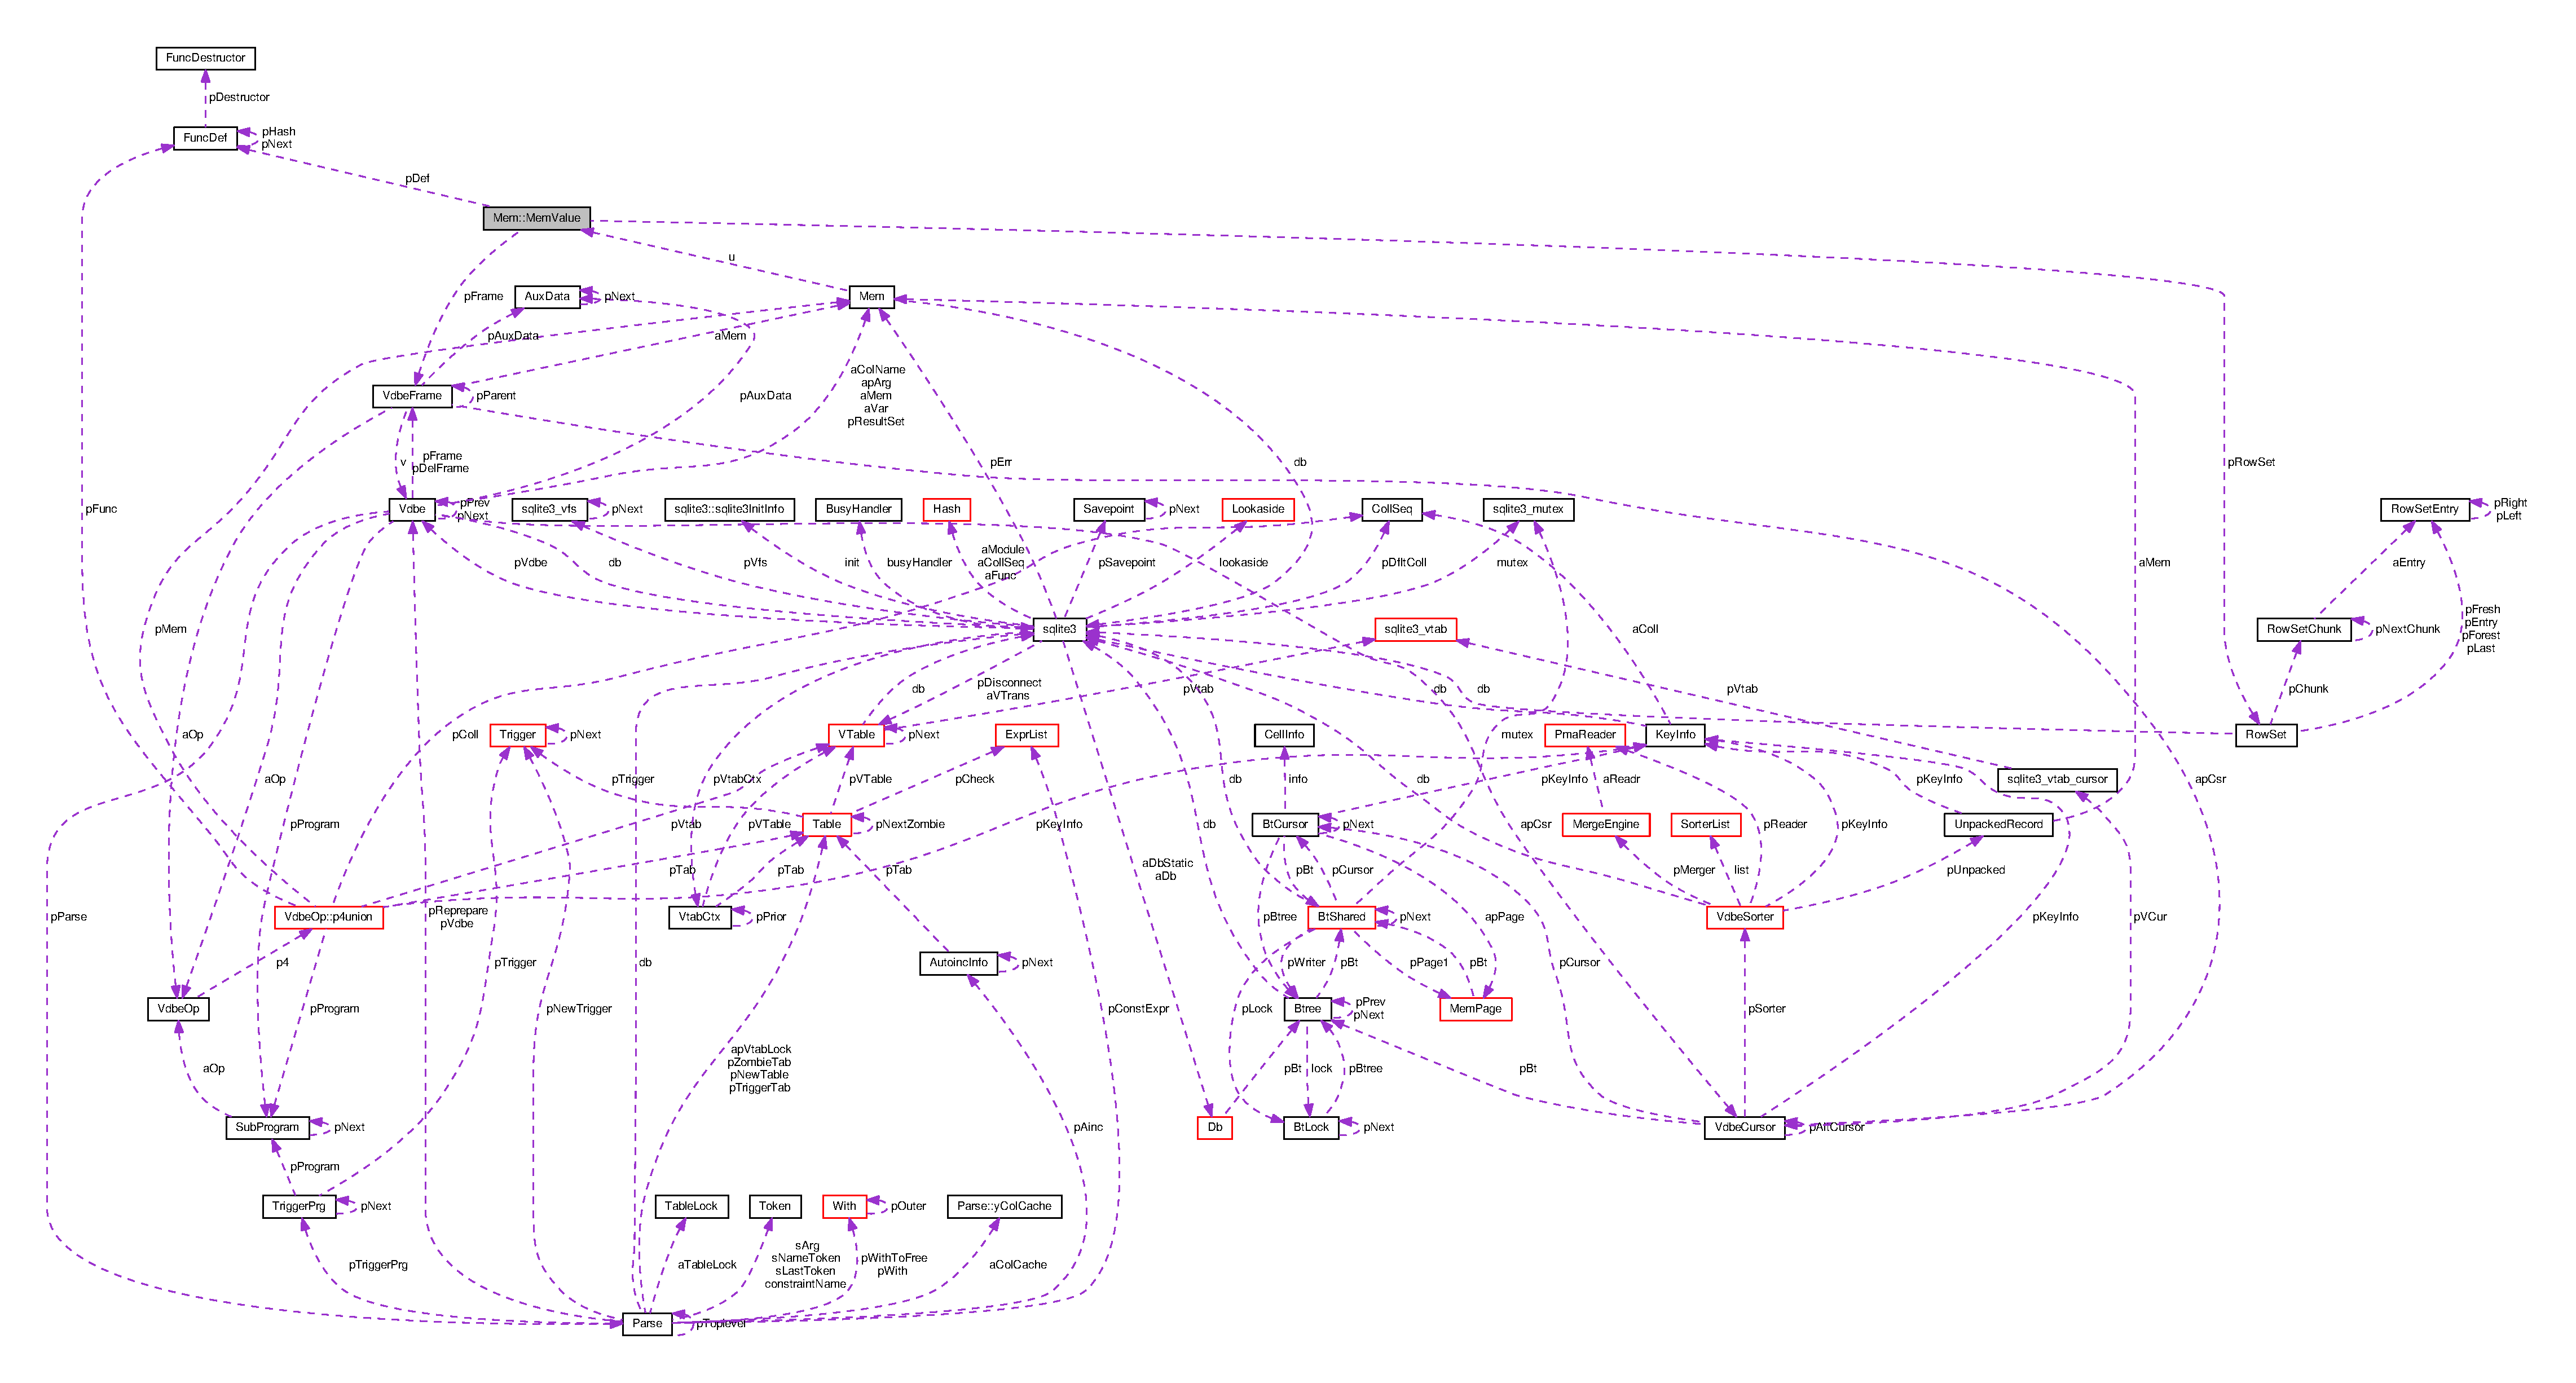
\includegraphics[width=350pt]{unionMem_1_1MemValue__coll__graph}
\end{center}
\end{figure}
\subsection*{Public Attributes}
\begin{DoxyCompactItemize}
\item 
double {\bfseries r}\hypertarget{unionMem_1_1MemValue_a1b30b01a5b7a3b337eeec4f39fb2a60c}{}\label{unionMem_1_1MemValue_a1b30b01a5b7a3b337eeec4f39fb2a60c}

\item 
i64 {\bfseries i}\hypertarget{unionMem_1_1MemValue_ac783c60cc4b1c0893931c997aa04ded6}{}\label{unionMem_1_1MemValue_ac783c60cc4b1c0893931c997aa04ded6}

\item 
int {\bfseries n\+Zero}\hypertarget{unionMem_1_1MemValue_a23976c454e79a60ca692305825792ca8}{}\label{unionMem_1_1MemValue_a23976c454e79a60ca692305825792ca8}

\item 
\hyperlink{structFuncDef}{Func\+Def} $\ast$ {\bfseries p\+Def}\hypertarget{unionMem_1_1MemValue_ad91c4fa3bebcc8bd9efa862841fd928d}{}\label{unionMem_1_1MemValue_ad91c4fa3bebcc8bd9efa862841fd928d}

\item 
\hyperlink{structRowSet}{Row\+Set} $\ast$ {\bfseries p\+Row\+Set}\hypertarget{unionMem_1_1MemValue_ab8b5abb605d926c611818285ecb3f7c5}{}\label{unionMem_1_1MemValue_ab8b5abb605d926c611818285ecb3f7c5}

\item 
\hyperlink{structVdbeFrame}{Vdbe\+Frame} $\ast$ {\bfseries p\+Frame}\hypertarget{unionMem_1_1MemValue_aa86f6085bfafd8a9ab3f41ac553f49fa}{}\label{unionMem_1_1MemValue_aa86f6085bfafd8a9ab3f41ac553f49fa}

\end{DoxyCompactItemize}


The documentation for this union was generated from the following file\+:\begin{DoxyCompactItemize}
\item 
sqlite3.\+c\end{DoxyCompactItemize}

\hypertarget{structMergeEngine}{}\section{Merge\+Engine Struct Reference}
\label{structMergeEngine}\index{Merge\+Engine@{Merge\+Engine}}


Collaboration diagram for Merge\+Engine\+:\nopagebreak
\begin{figure}[H]
\begin{center}
\leavevmode
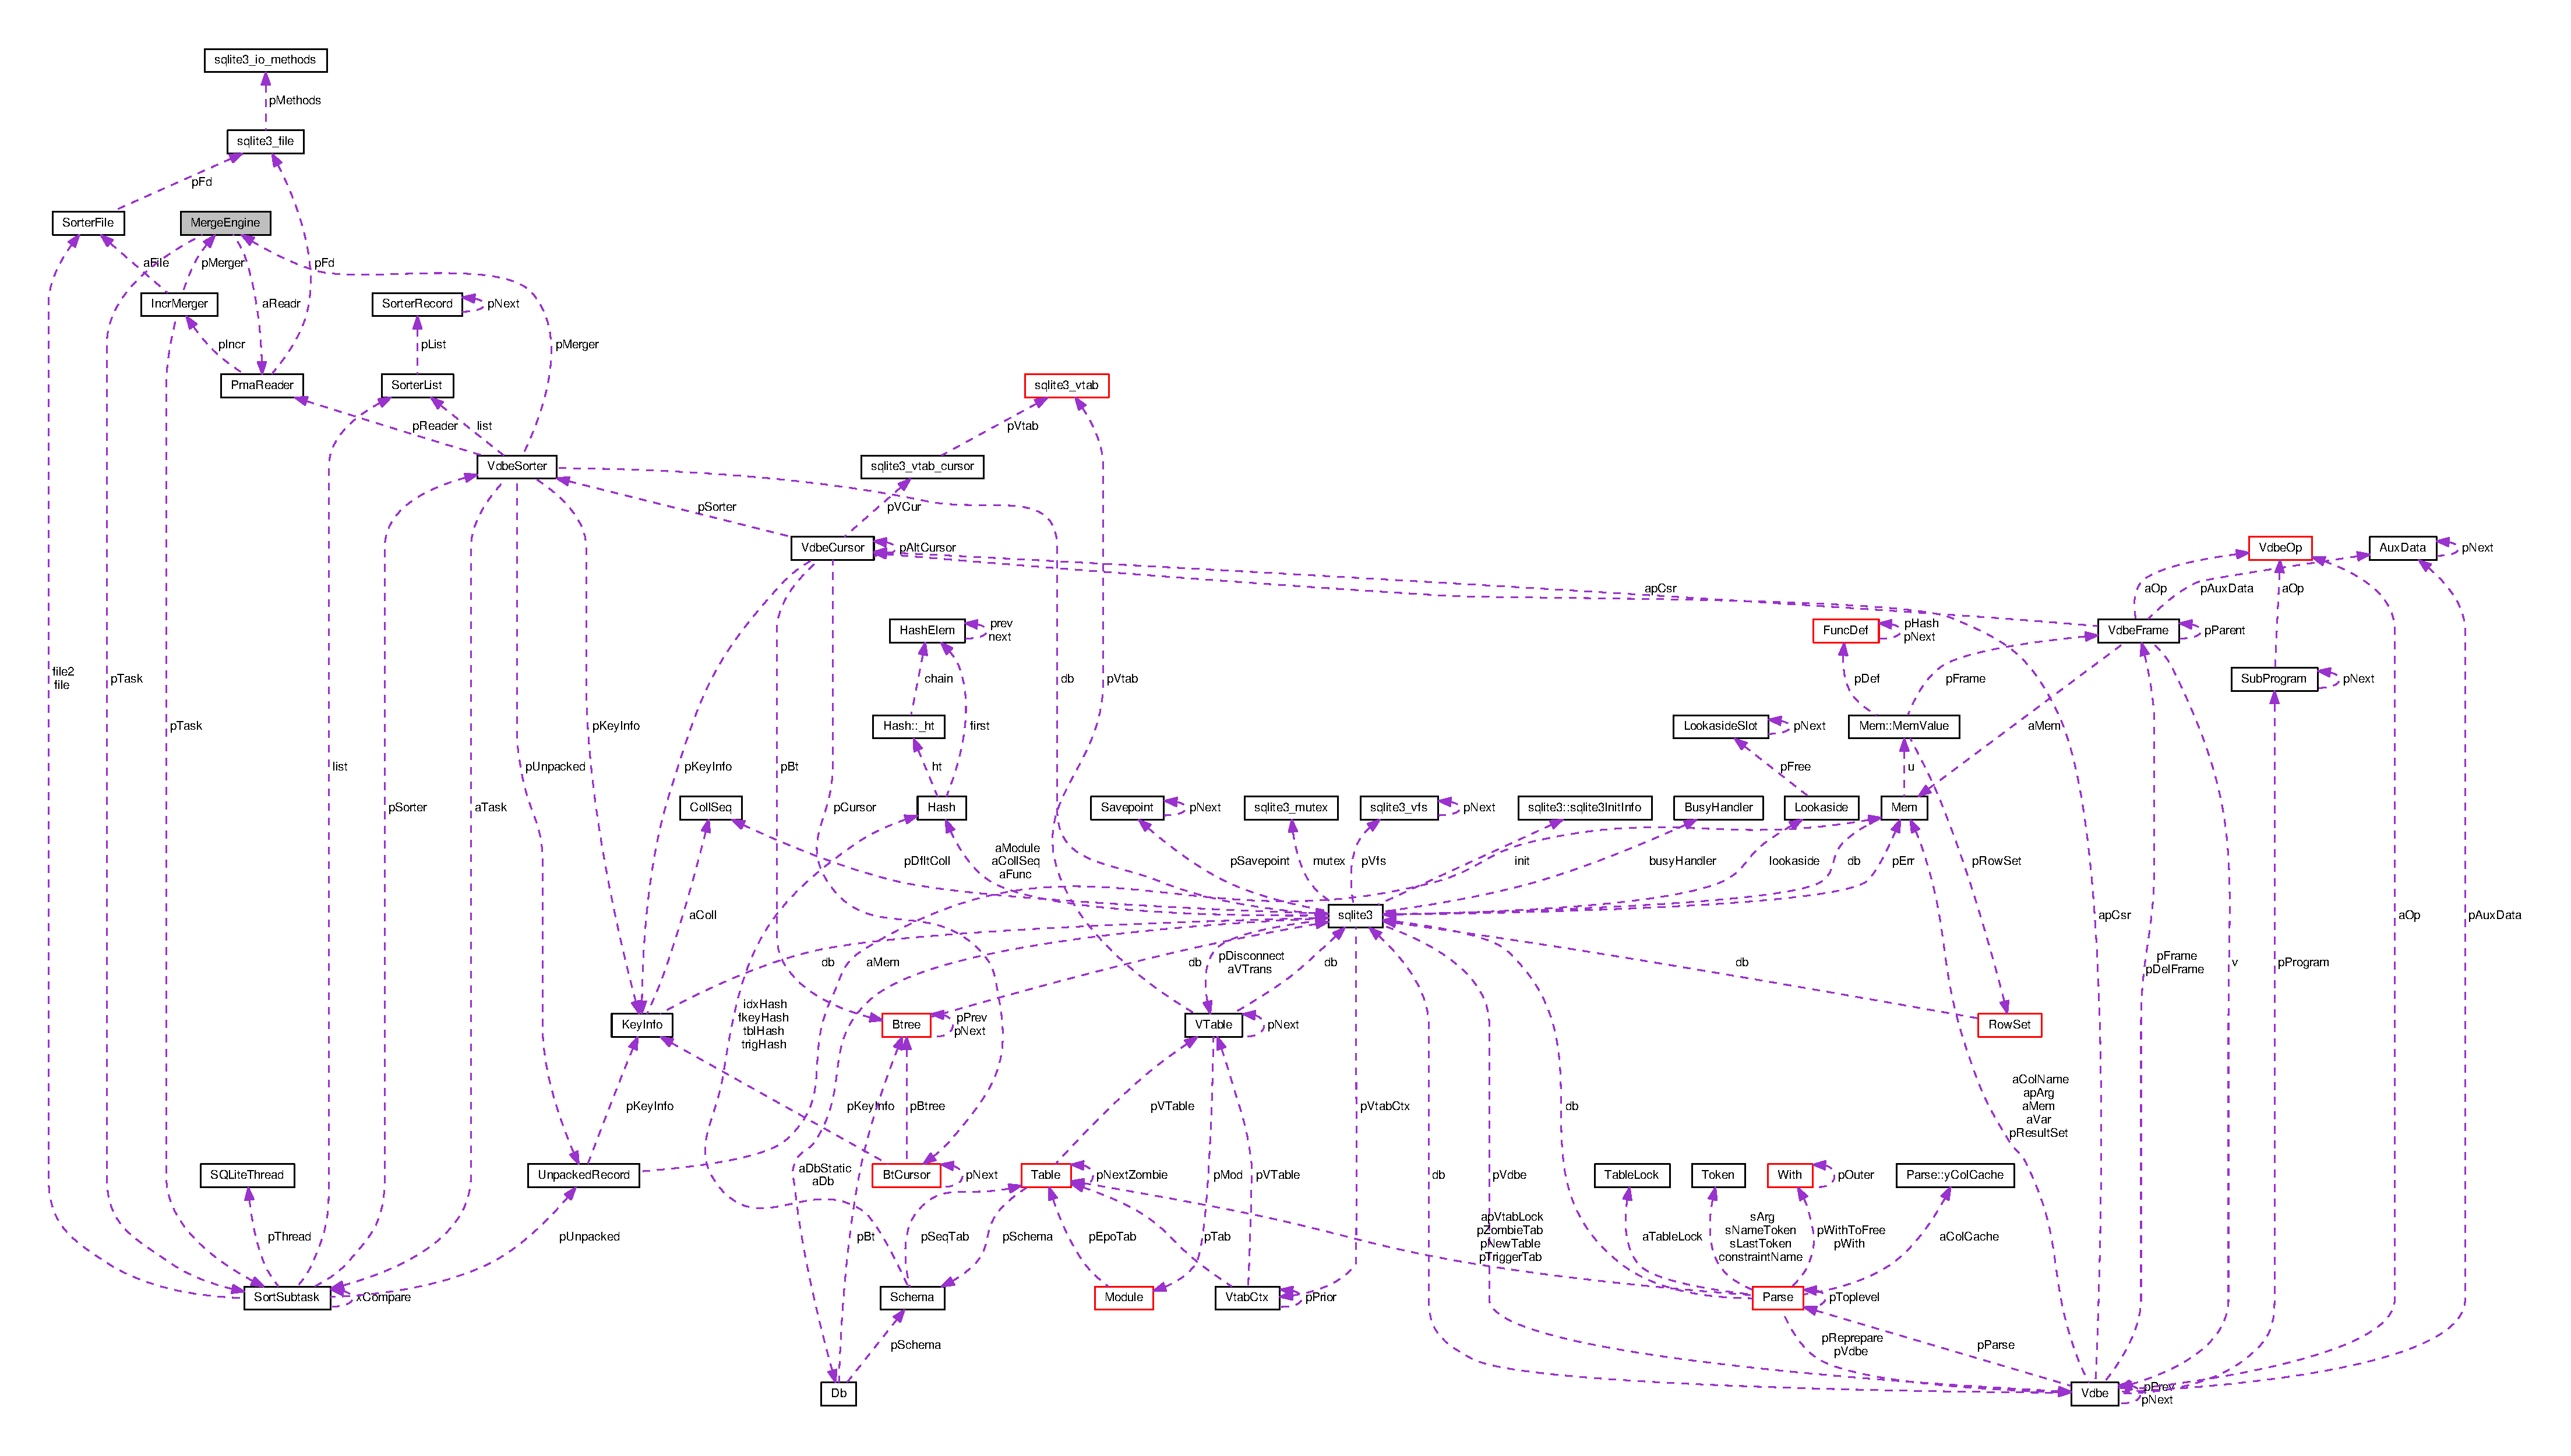
\includegraphics[width=350pt]{structMergeEngine__coll__graph}
\end{center}
\end{figure}
\subsection*{Public Attributes}
\begin{DoxyCompactItemize}
\item 
int {\bfseries n\+Tree}\hypertarget{structMergeEngine_a48d8ad99ae5063e96458b5563ff2bbd3}{}\label{structMergeEngine_a48d8ad99ae5063e96458b5563ff2bbd3}

\item 
\hyperlink{structSortSubtask}{Sort\+Subtask} $\ast$ {\bfseries p\+Task}\hypertarget{structMergeEngine_a0a366796f579aa7befcb2683ff767c0d}{}\label{structMergeEngine_a0a366796f579aa7befcb2683ff767c0d}

\item 
int $\ast$ {\bfseries a\+Tree}\hypertarget{structMergeEngine_aac39bb928db1c72c48db263e0937b285}{}\label{structMergeEngine_aac39bb928db1c72c48db263e0937b285}

\item 
\hyperlink{structPmaReader}{Pma\+Reader} $\ast$ {\bfseries a\+Readr}\hypertarget{structMergeEngine_a897688db3212c8b3049a57cda6f2f975}{}\label{structMergeEngine_a897688db3212c8b3049a57cda6f2f975}

\end{DoxyCompactItemize}


The documentation for this struct was generated from the following file\+:\begin{DoxyCompactItemize}
\item 
sqlite3.\+c\end{DoxyCompactItemize}

\hypertarget{structModule}{}\section{Module Struct Reference}
\label{structModule}\index{Module@{Module}}


Collaboration diagram for Module\+:
% FIG 0
\subsection*{Public Attributes}
\begin{DoxyCompactItemize}
\item 
const \hyperlink{structsqlite3__module}{sqlite3\+\_\+module} $\ast$ {\bfseries p\+Module}\hypertarget{structModule_a65d2539d71ea028b505b2fb33563bfd7}{}\label{structModule_a65d2539d71ea028b505b2fb33563bfd7}

\item 
const char $\ast$ {\bfseries z\+Name}\hypertarget{structModule_a45a5f5b43926b8ebf3e13e46a6534810}{}\label{structModule_a45a5f5b43926b8ebf3e13e46a6534810}

\item 
void $\ast$ {\bfseries p\+Aux}\hypertarget{structModule_ae3b827fee4c8b4f3ff38c86c2e2f48cd}{}\label{structModule_ae3b827fee4c8b4f3ff38c86c2e2f48cd}

\item 
void($\ast$ {\bfseries x\+Destroy} )(void $\ast$)\hypertarget{structModule_a4a4b707d6ad852cf2e8d983d22886cc1}{}\label{structModule_a4a4b707d6ad852cf2e8d983d22886cc1}

\item 
\hyperlink{structTable}{Table} $\ast$ {\bfseries p\+Epo\+Tab}\hypertarget{structModule_a546d1d825743f3083e7413f9f280d402}{}\label{structModule_a546d1d825743f3083e7413f9f280d402}

\end{DoxyCompactItemize}


The documentation for this struct was generated from the following file\+:\begin{DoxyCompactItemize}
\item 
sqlite3.\+c\end{DoxyCompactItemize}

\hypertarget{structNameContext}{}\section{Name\+Context Struct Reference}
\label{structNameContext}\index{Name\+Context@{Name\+Context}}


Collaboration diagram for Name\+Context\+:
% FIG 0
\subsection*{Public Attributes}
\begin{DoxyCompactItemize}
\item 
\hyperlink{structParse}{Parse} $\ast$ {\bfseries p\+Parse}\hypertarget{structNameContext_a14635249bf75d5e18124089571dd2386}{}\label{structNameContext_a14635249bf75d5e18124089571dd2386}

\item 
\hyperlink{structSrcList}{Src\+List} $\ast$ {\bfseries p\+Src\+List}\hypertarget{structNameContext_a6ede21da33e2e9bd3d0c5fe90a3ec72c}{}\label{structNameContext_a6ede21da33e2e9bd3d0c5fe90a3ec72c}

\item 
\hyperlink{structExprList}{Expr\+List} $\ast$ {\bfseries p\+E\+List}\hypertarget{structNameContext_a8c752d7fb9b28179156c569cc57ba6f2}{}\label{structNameContext_a8c752d7fb9b28179156c569cc57ba6f2}

\item 
\hyperlink{structAggInfo}{Agg\+Info} $\ast$ {\bfseries p\+Agg\+Info}\hypertarget{structNameContext_aeb3ff72c03dd770d421cadc2195a5644}{}\label{structNameContext_aeb3ff72c03dd770d421cadc2195a5644}

\item 
\hyperlink{structNameContext}{Name\+Context} $\ast$ {\bfseries p\+Next}\hypertarget{structNameContext_a82ce0ec8a3cc3d792e1f38bb5e0ad5fc}{}\label{structNameContext_a82ce0ec8a3cc3d792e1f38bb5e0ad5fc}

\item 
int {\bfseries n\+Ref}\hypertarget{structNameContext_ad68616ce2a58fa1b135e0dcf953bdc97}{}\label{structNameContext_ad68616ce2a58fa1b135e0dcf953bdc97}

\item 
int {\bfseries n\+Err}\hypertarget{structNameContext_aba0b89b42e945c4c96d57a8fe011329c}{}\label{structNameContext_aba0b89b42e945c4c96d57a8fe011329c}

\item 
u16 {\bfseries nc\+Flags}\hypertarget{structNameContext_af1721ec037371cabc7385822cbd9629a}{}\label{structNameContext_af1721ec037371cabc7385822cbd9629a}

\end{DoxyCompactItemize}


The documentation for this struct was generated from the following file\+:\begin{DoxyCompactItemize}
\item 
sqlite3.\+c\end{DoxyCompactItemize}

\hypertarget{unionVdbeOp_1_1p4union}{}\section{Vdbe\+Op\+:\+:p4union Union Reference}
\label{unionVdbeOp_1_1p4union}\index{Vdbe\+Op\+::p4union@{Vdbe\+Op\+::p4union}}


Collaboration diagram for Vdbe\+Op\+:\+:p4union\+:\nopagebreak
\begin{figure}[H]
\begin{center}
\leavevmode
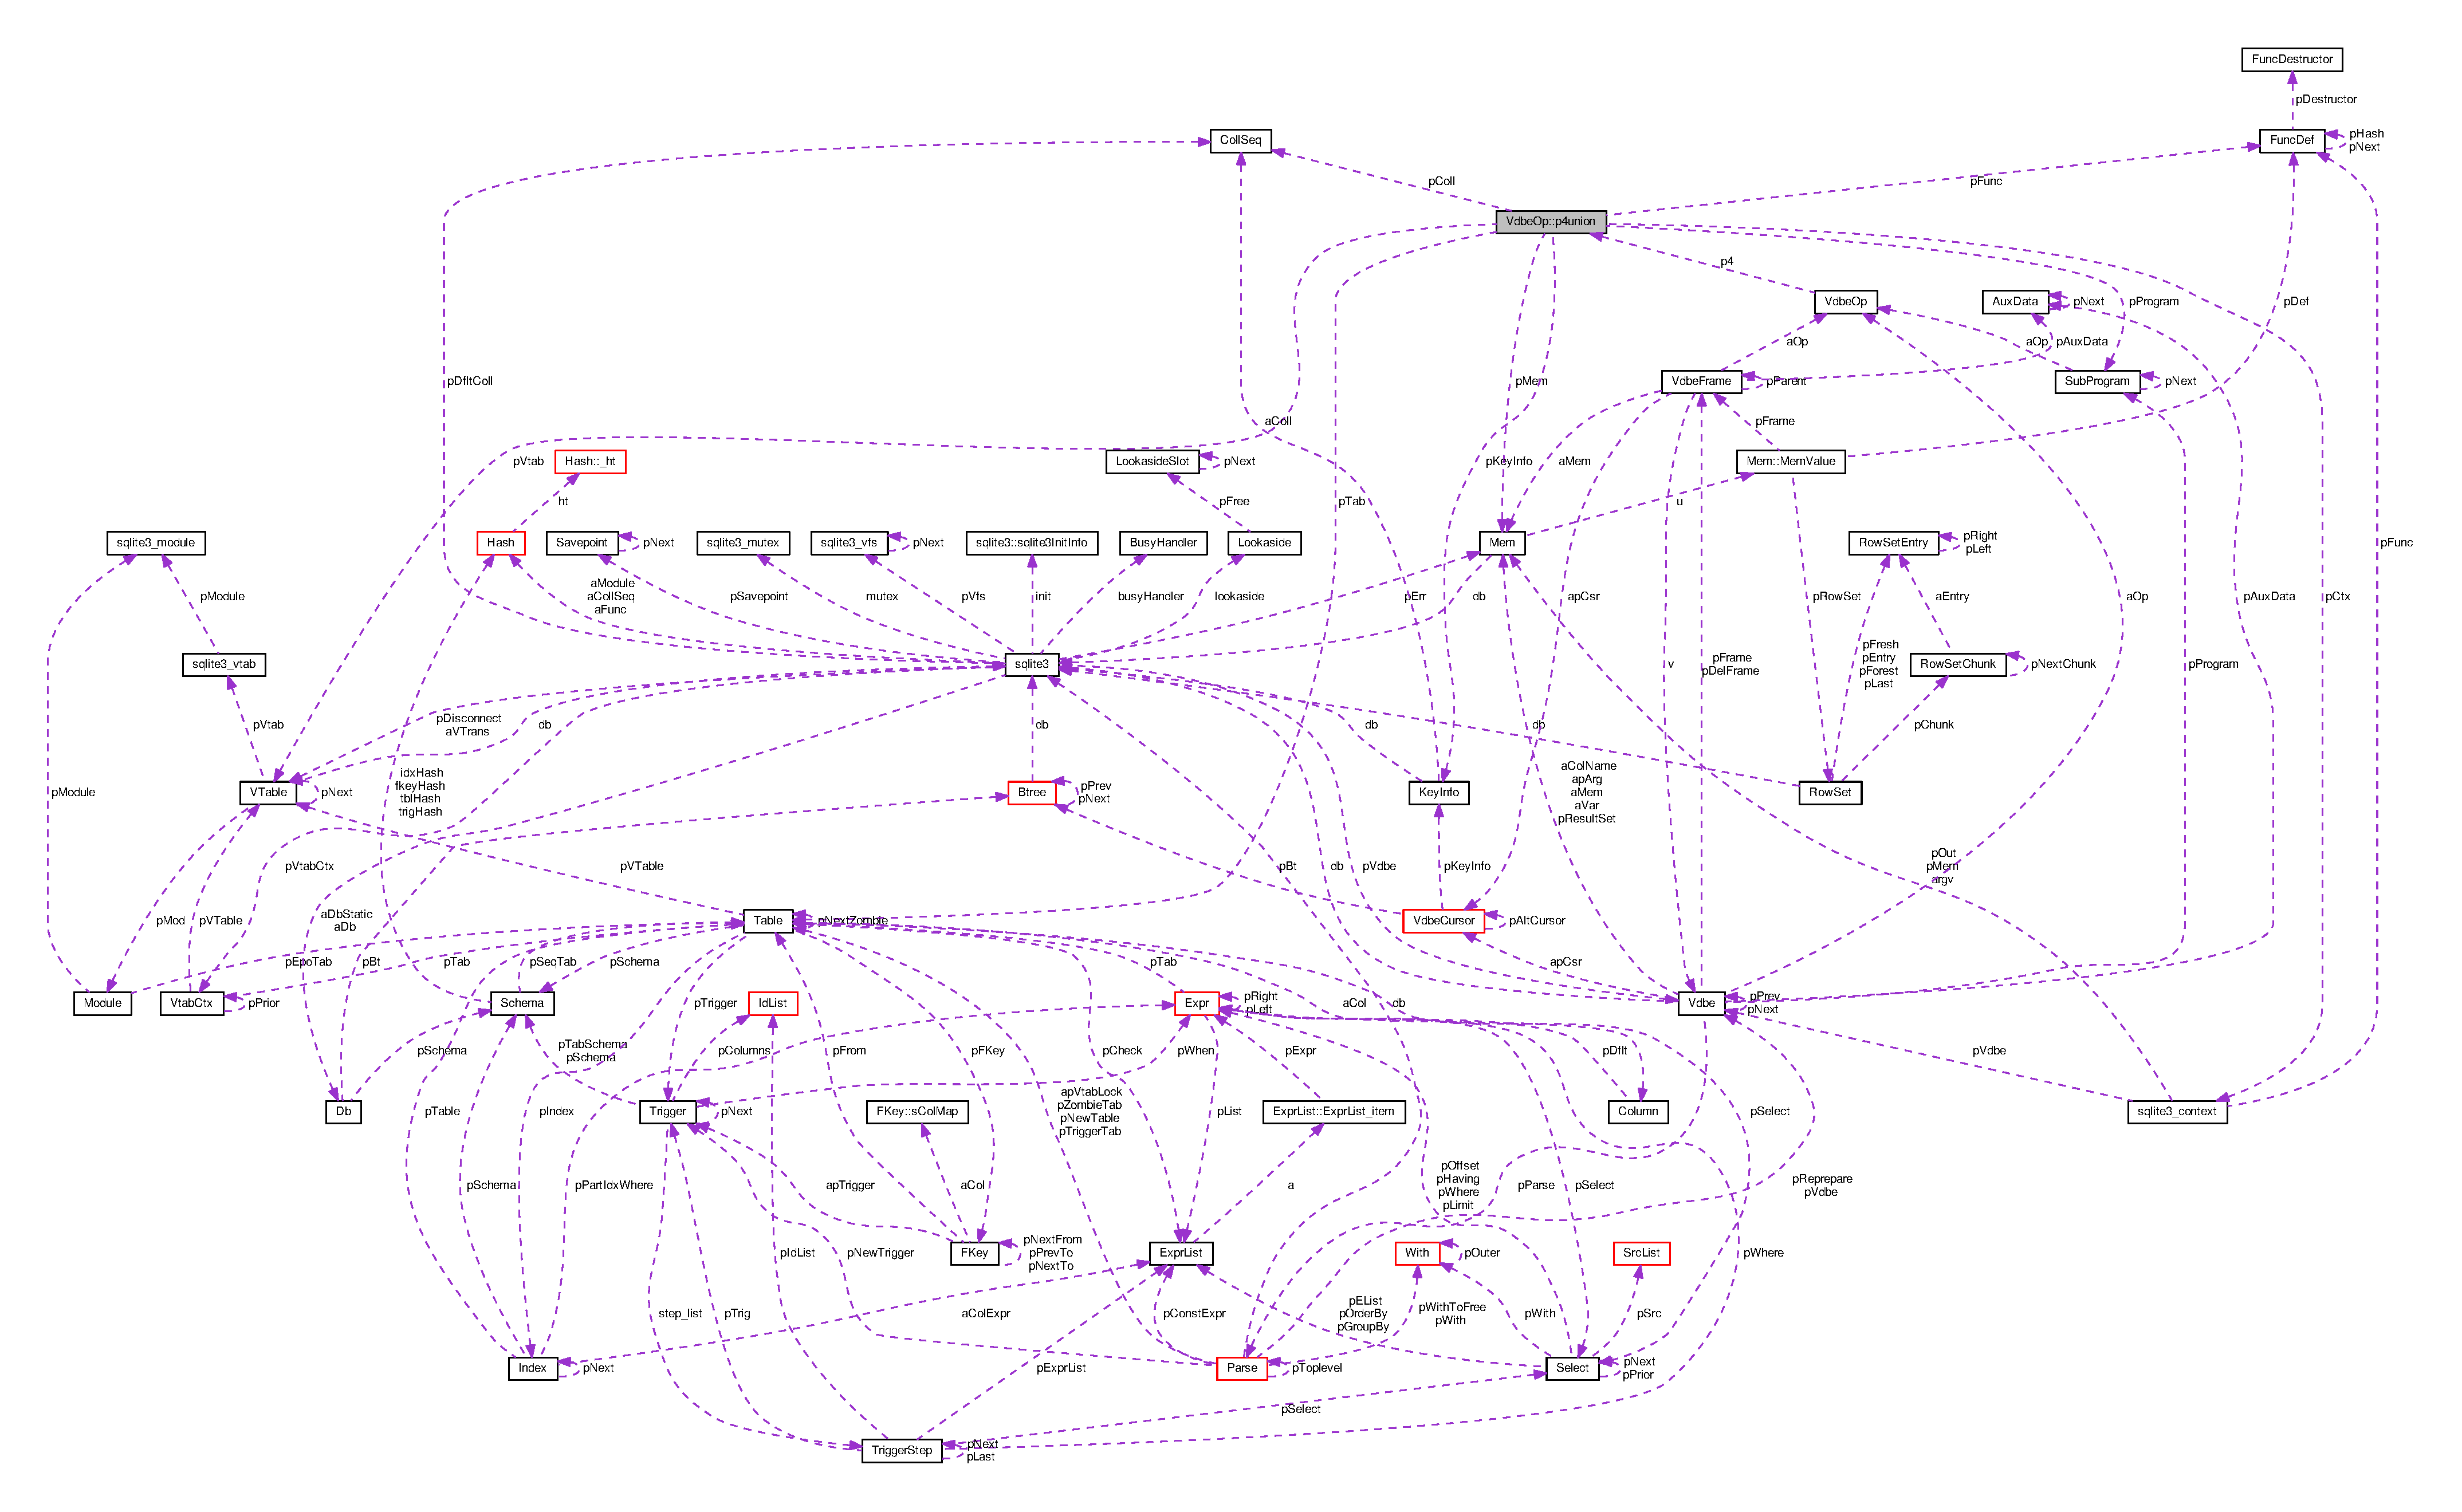
\includegraphics[width=350pt]{unionVdbeOp_1_1p4union__coll__graph}
\end{center}
\end{figure}
\subsection*{Public Attributes}
\begin{DoxyCompactItemize}
\item 
int {\bfseries i}\hypertarget{unionVdbeOp_1_1p4union_a67b1d33cd04d43500226f2fc5cd0c6c4}{}\label{unionVdbeOp_1_1p4union_a67b1d33cd04d43500226f2fc5cd0c6c4}

\item 
void $\ast$ {\bfseries p}\hypertarget{unionVdbeOp_1_1p4union_a084b1849db2067d5aa349e3988d2f515}{}\label{unionVdbeOp_1_1p4union_a084b1849db2067d5aa349e3988d2f515}

\item 
char $\ast$ {\bfseries z}\hypertarget{unionVdbeOp_1_1p4union_ab679a57e8d973f81a8d51f925502d430}{}\label{unionVdbeOp_1_1p4union_ab679a57e8d973f81a8d51f925502d430}

\item 
i64 $\ast$ {\bfseries p\+I64}\hypertarget{unionVdbeOp_1_1p4union_a6058dda6de49e297bc89e53060e97354}{}\label{unionVdbeOp_1_1p4union_a6058dda6de49e297bc89e53060e97354}

\item 
double $\ast$ {\bfseries p\+Real}\hypertarget{unionVdbeOp_1_1p4union_a39e6887128786424eaf8dc31e7a88f66}{}\label{unionVdbeOp_1_1p4union_a39e6887128786424eaf8dc31e7a88f66}

\item 
\hyperlink{structFuncDef}{Func\+Def} $\ast$ {\bfseries p\+Func}\hypertarget{unionVdbeOp_1_1p4union_a6832dea5d3721f13f718592de2bc9b23}{}\label{unionVdbeOp_1_1p4union_a6832dea5d3721f13f718592de2bc9b23}

\item 
\hyperlink{structsqlite3__context}{sqlite3\+\_\+context} $\ast$ {\bfseries p\+Ctx}\hypertarget{unionVdbeOp_1_1p4union_aa1ca37d471aef629b85a8b3c628faa06}{}\label{unionVdbeOp_1_1p4union_aa1ca37d471aef629b85a8b3c628faa06}

\item 
\hyperlink{structCollSeq}{Coll\+Seq} $\ast$ {\bfseries p\+Coll}\hypertarget{unionVdbeOp_1_1p4union_abdd570179d6f6428b96d56b0292f068b}{}\label{unionVdbeOp_1_1p4union_abdd570179d6f6428b96d56b0292f068b}

\item 
\hyperlink{structMem}{Mem} $\ast$ {\bfseries p\+Mem}\hypertarget{unionVdbeOp_1_1p4union_a52d756a2ccc11e5e87703e6f8129261c}{}\label{unionVdbeOp_1_1p4union_a52d756a2ccc11e5e87703e6f8129261c}

\item 
\hyperlink{structVTable}{V\+Table} $\ast$ {\bfseries p\+Vtab}\hypertarget{unionVdbeOp_1_1p4union_a25abd8bcf2df2f591e2dc6c377f8f427}{}\label{unionVdbeOp_1_1p4union_a25abd8bcf2df2f591e2dc6c377f8f427}

\item 
\hyperlink{structKeyInfo}{Key\+Info} $\ast$ {\bfseries p\+Key\+Info}\hypertarget{unionVdbeOp_1_1p4union_acda5935a8938d01e523d0eb79b0c1e72}{}\label{unionVdbeOp_1_1p4union_acda5935a8938d01e523d0eb79b0c1e72}

\item 
int $\ast$ {\bfseries ai}\hypertarget{unionVdbeOp_1_1p4union_a1bd30fbce8b173d7270d04dc714863f3}{}\label{unionVdbeOp_1_1p4union_a1bd30fbce8b173d7270d04dc714863f3}

\item 
\hyperlink{structSubProgram}{Sub\+Program} $\ast$ {\bfseries p\+Program}\hypertarget{unionVdbeOp_1_1p4union_ac72a98a54ea6ddd7b168af47fab46a41}{}\label{unionVdbeOp_1_1p4union_ac72a98a54ea6ddd7b168af47fab46a41}

\item 
\hyperlink{structTable}{Table} $\ast$ {\bfseries p\+Tab}\hypertarget{unionVdbeOp_1_1p4union_af846307afcc87ba2ca357108d3c48edf}{}\label{unionVdbeOp_1_1p4union_af846307afcc87ba2ca357108d3c48edf}

\item 
int($\ast$ {\bfseries x\+Advance} )(\hyperlink{structBtCursor}{Bt\+Cursor} $\ast$, int $\ast$)\hypertarget{unionVdbeOp_1_1p4union_abede37475ebf4b3c05a43cef11281f4e}{}\label{unionVdbeOp_1_1p4union_abede37475ebf4b3c05a43cef11281f4e}

\end{DoxyCompactItemize}


The documentation for this union was generated from the following file\+:\begin{DoxyCompactItemize}
\item 
sqlite3.\+c\end{DoxyCompactItemize}

\hypertarget{classPackage}{}\section{Package Class Reference}
\label{classPackage}\index{Package@{Package}}


\hyperlink{classPackage}{Package} class.  




{\ttfamily \#include $<$Package.\+h$>$}

\subsection*{Public Types}
\begin{DoxyCompactItemize}
\item 
enum {\bfseries Priority} \{ {\bfseries R\+E\+G\+U\+L\+AR}, 
{\bfseries T\+W\+O\+\_\+\+D\+AY}, 
{\bfseries O\+V\+E\+R\+N\+I\+G\+HT}
 \}\hypertarget{classPackage_ac96ebcf78f2d93898635a1275da0c0bd}{}\label{classPackage_ac96ebcf78f2d93898635a1275da0c0bd}

\end{DoxyCompactItemize}
\subsection*{Public Member Functions}
\begin{DoxyCompactItemize}
\item 
\hyperlink{classPackage_a64d987fe7cb1d583f2af4a38e544a6f2}{Package} (\hyperlink{classClient}{Client} $\ast$, \hyperlink{classClient}{Client} $\ast$, const double, const Priority)
\begin{DoxyCompactList}\small\item\em Constructor. \end{DoxyCompactList}\item 
void \hyperlink{classPackage_a933801e98e91c1d540f9a47926bfc314}{set\+Sender} (\hyperlink{classClient}{Client} $\ast$)
\begin{DoxyCompactList}\small\item\em Sender setter. \end{DoxyCompactList}\item 
\hyperlink{classClient}{Client} $\ast$ \hyperlink{classPackage_a1e603126edbbd5c82c676eb0e6805554}{get\+Sender} () const 
\begin{DoxyCompactList}\small\item\em Sender getter. \end{DoxyCompactList}\item 
void \hyperlink{classPackage_a6a16574423734d7fd0aa4d5a74b0ad32}{set\+Receiver} (\hyperlink{classClient}{Client} $\ast$)
\begin{DoxyCompactList}\small\item\em Receiver setter. \end{DoxyCompactList}\item 
\hyperlink{classClient}{Client} $\ast$ \hyperlink{classPackage_a02e9aee9f9e10b6b6ba124df61bd289d}{get\+Receiver} () const 
\begin{DoxyCompactList}\small\item\em Receiver getter. \end{DoxyCompactList}\item 
void \hyperlink{classPackage_a0766f8a791e0b76d97671cb92d785496}{set\+Weight} (const double)
\begin{DoxyCompactList}\small\item\em Weight setter. \end{DoxyCompactList}\item 
double \hyperlink{classPackage_a2da083a8cab4c978c22c49ac46226aee}{get\+Weight} () const 
\begin{DoxyCompactList}\small\item\em Weight getter. \end{DoxyCompactList}\item 
void \hyperlink{classPackage_afe16b4fbff0a050019ddf47978001464}{set\+Priority} (const Priority)
\begin{DoxyCompactList}\small\item\em Priority setter. \end{DoxyCompactList}\item 
Priority \hyperlink{classPackage_accf52df9d08053e7c1c126d747e6beb0}{get\+Priority} () const 
\begin{DoxyCompactList}\small\item\em Priority getter. \end{DoxyCompactList}\end{DoxyCompactItemize}


\subsection{Detailed Description}
\hyperlink{classPackage}{Package} class. 

This \hyperlink{classPackage}{Package} class defines a package which was sent by a \hyperlink{classClient}{Client} and received by a \hyperlink{classClient}{Client}. Each package has a priority, a weight, and two clients (a sender and receiver). 

\subsection{Constructor \& Destructor Documentation}
\index{Package@{Package}!Package@{Package}}
\index{Package@{Package}!Package@{Package}}
\subsubsection[{\texorpdfstring{Package(\+Client $\ast$, Client $\ast$, const double, const Priority)}{Package(Client *, Client *, const double, const Priority)}}]{\setlength{\rightskip}{0pt plus 5cm}Package\+::\+Package (
\begin{DoxyParamCaption}
\item[{{\bf Client} $\ast$}]{s, }
\item[{{\bf Client} $\ast$}]{r, }
\item[{const double}]{w, }
\item[{const Priority}]{p}
\end{DoxyParamCaption}
)}\hypertarget{classPackage_a64d987fe7cb1d583f2af4a38e544a6f2}{}\label{classPackage_a64d987fe7cb1d583f2af4a38e544a6f2}


Constructor. 


\begin{DoxyParams}{Parameters}
{\em s} & Sender \hyperlink{classClient}{Client} \\
\hline
{\em r} & Receiver \hyperlink{classClient}{Client} \\
\hline
{\em w} & \hyperlink{classPackage}{Package} weight \\
\hline
{\em p} & \hyperlink{classPackage}{Package} priority \\
\hline
\end{DoxyParams}


\subsection{Member Function Documentation}
\index{Package@{Package}!get\+Priority@{get\+Priority}}
\index{get\+Priority@{get\+Priority}!Package@{Package}}
\subsubsection[{\texorpdfstring{get\+Priority() const }{getPriority() const }}]{\setlength{\rightskip}{0pt plus 5cm}Package\+::\+Priority Package\+::get\+Priority (
\begin{DoxyParamCaption}
{}
\end{DoxyParamCaption}
) const}\hypertarget{classPackage_accf52df9d08053e7c1c126d747e6beb0}{}\label{classPackage_accf52df9d08053e7c1c126d747e6beb0}


Priority getter. 

\hyperlink{classPackage}{Package} priority getter.

\begin{DoxyReturn}{Returns}
\hyperlink{classPackage}{Package} priority 
\end{DoxyReturn}
\index{Package@{Package}!get\+Receiver@{get\+Receiver}}
\index{get\+Receiver@{get\+Receiver}!Package@{Package}}
\subsubsection[{\texorpdfstring{get\+Receiver() const }{getReceiver() const }}]{\setlength{\rightskip}{0pt plus 5cm}{\bf Client} $\ast$ Package\+::get\+Receiver (
\begin{DoxyParamCaption}
{}
\end{DoxyParamCaption}
) const}\hypertarget{classPackage_a02e9aee9f9e10b6b6ba124df61bd289d}{}\label{classPackage_a02e9aee9f9e10b6b6ba124df61bd289d}


Receiver getter. 

\begin{DoxyReturn}{Returns}
pointer to receiver client 
\end{DoxyReturn}
\index{Package@{Package}!get\+Sender@{get\+Sender}}
\index{get\+Sender@{get\+Sender}!Package@{Package}}
\subsubsection[{\texorpdfstring{get\+Sender() const }{getSender() const }}]{\setlength{\rightskip}{0pt plus 5cm}{\bf Client} $\ast$ Package\+::get\+Sender (
\begin{DoxyParamCaption}
{}
\end{DoxyParamCaption}
) const}\hypertarget{classPackage_a1e603126edbbd5c82c676eb0e6805554}{}\label{classPackage_a1e603126edbbd5c82c676eb0e6805554}


Sender getter. 

\begin{DoxyReturn}{Returns}
pointer to sender client 
\end{DoxyReturn}
\index{Package@{Package}!get\+Weight@{get\+Weight}}
\index{get\+Weight@{get\+Weight}!Package@{Package}}
\subsubsection[{\texorpdfstring{get\+Weight() const }{getWeight() const }}]{\setlength{\rightskip}{0pt plus 5cm}double Package\+::get\+Weight (
\begin{DoxyParamCaption}
{}
\end{DoxyParamCaption}
) const}\hypertarget{classPackage_a2da083a8cab4c978c22c49ac46226aee}{}\label{classPackage_a2da083a8cab4c978c22c49ac46226aee}


Weight getter. 

\hyperlink{classPackage}{Package} Weight getter.

\begin{DoxyReturn}{Returns}
\hyperlink{classPackage}{Package} weight 
\end{DoxyReturn}
\index{Package@{Package}!set\+Priority@{set\+Priority}}
\index{set\+Priority@{set\+Priority}!Package@{Package}}
\subsubsection[{\texorpdfstring{set\+Priority(const Priority)}{setPriority(const Priority)}}]{\setlength{\rightskip}{0pt plus 5cm}void Package\+::set\+Priority (
\begin{DoxyParamCaption}
\item[{const Priority}]{p}
\end{DoxyParamCaption}
)}\hypertarget{classPackage_afe16b4fbff0a050019ddf47978001464}{}\label{classPackage_afe16b4fbff0a050019ddf47978001464}


Priority setter. 

\hyperlink{classPackage}{Package} Priority setter.


\begin{DoxyParams}{Parameters}
{\em p} & Priority enum \\
\hline
\end{DoxyParams}
\index{Package@{Package}!set\+Receiver@{set\+Receiver}}
\index{set\+Receiver@{set\+Receiver}!Package@{Package}}
\subsubsection[{\texorpdfstring{set\+Receiver(\+Client $\ast$)}{setReceiver(Client *)}}]{\setlength{\rightskip}{0pt plus 5cm}void Package\+::set\+Receiver (
\begin{DoxyParamCaption}
\item[{{\bf Client} $\ast$}]{r}
\end{DoxyParamCaption}
)}\hypertarget{classPackage_a6a16574423734d7fd0aa4d5a74b0ad32}{}\label{classPackage_a6a16574423734d7fd0aa4d5a74b0ad32}


Receiver setter. 


\begin{DoxyParams}{Parameters}
{\em r} & pointer to receiver client \\
\hline
\end{DoxyParams}
\index{Package@{Package}!set\+Sender@{set\+Sender}}
\index{set\+Sender@{set\+Sender}!Package@{Package}}
\subsubsection[{\texorpdfstring{set\+Sender(\+Client $\ast$)}{setSender(Client *)}}]{\setlength{\rightskip}{0pt plus 5cm}void Package\+::set\+Sender (
\begin{DoxyParamCaption}
\item[{{\bf Client} $\ast$}]{s}
\end{DoxyParamCaption}
)}\hypertarget{classPackage_a933801e98e91c1d540f9a47926bfc314}{}\label{classPackage_a933801e98e91c1d540f9a47926bfc314}


Sender setter. 


\begin{DoxyParams}{Parameters}
{\em s} & pointer to sender client \\
\hline
\end{DoxyParams}
\index{Package@{Package}!set\+Weight@{set\+Weight}}
\index{set\+Weight@{set\+Weight}!Package@{Package}}
\subsubsection[{\texorpdfstring{set\+Weight(const double)}{setWeight(const double)}}]{\setlength{\rightskip}{0pt plus 5cm}void Package\+::set\+Weight (
\begin{DoxyParamCaption}
\item[{const double}]{w}
\end{DoxyParamCaption}
)}\hypertarget{classPackage_a0766f8a791e0b76d97671cb92d785496}{}\label{classPackage_a0766f8a791e0b76d97671cb92d785496}


Weight setter. 

\hyperlink{classPackage}{Package} weight setter.

Throws error on negative weight. 
\begin{DoxyParams}{Parameters}
{\em w} & \hyperlink{classPackage}{Package} weight \\
\hline
\end{DoxyParams}


The documentation for this class was generated from the following files\+:\begin{DoxyCompactItemize}
\item 
Package.\+h\item 
Package.\+cpp\end{DoxyCompactItemize}

\hypertarget{structPager}{}\section{Pager Struct Reference}
\label{structPager}\index{Pager@{Pager}}


Collaboration diagram for Pager\+:\nopagebreak
\begin{figure}[H]
\begin{center}
\leavevmode
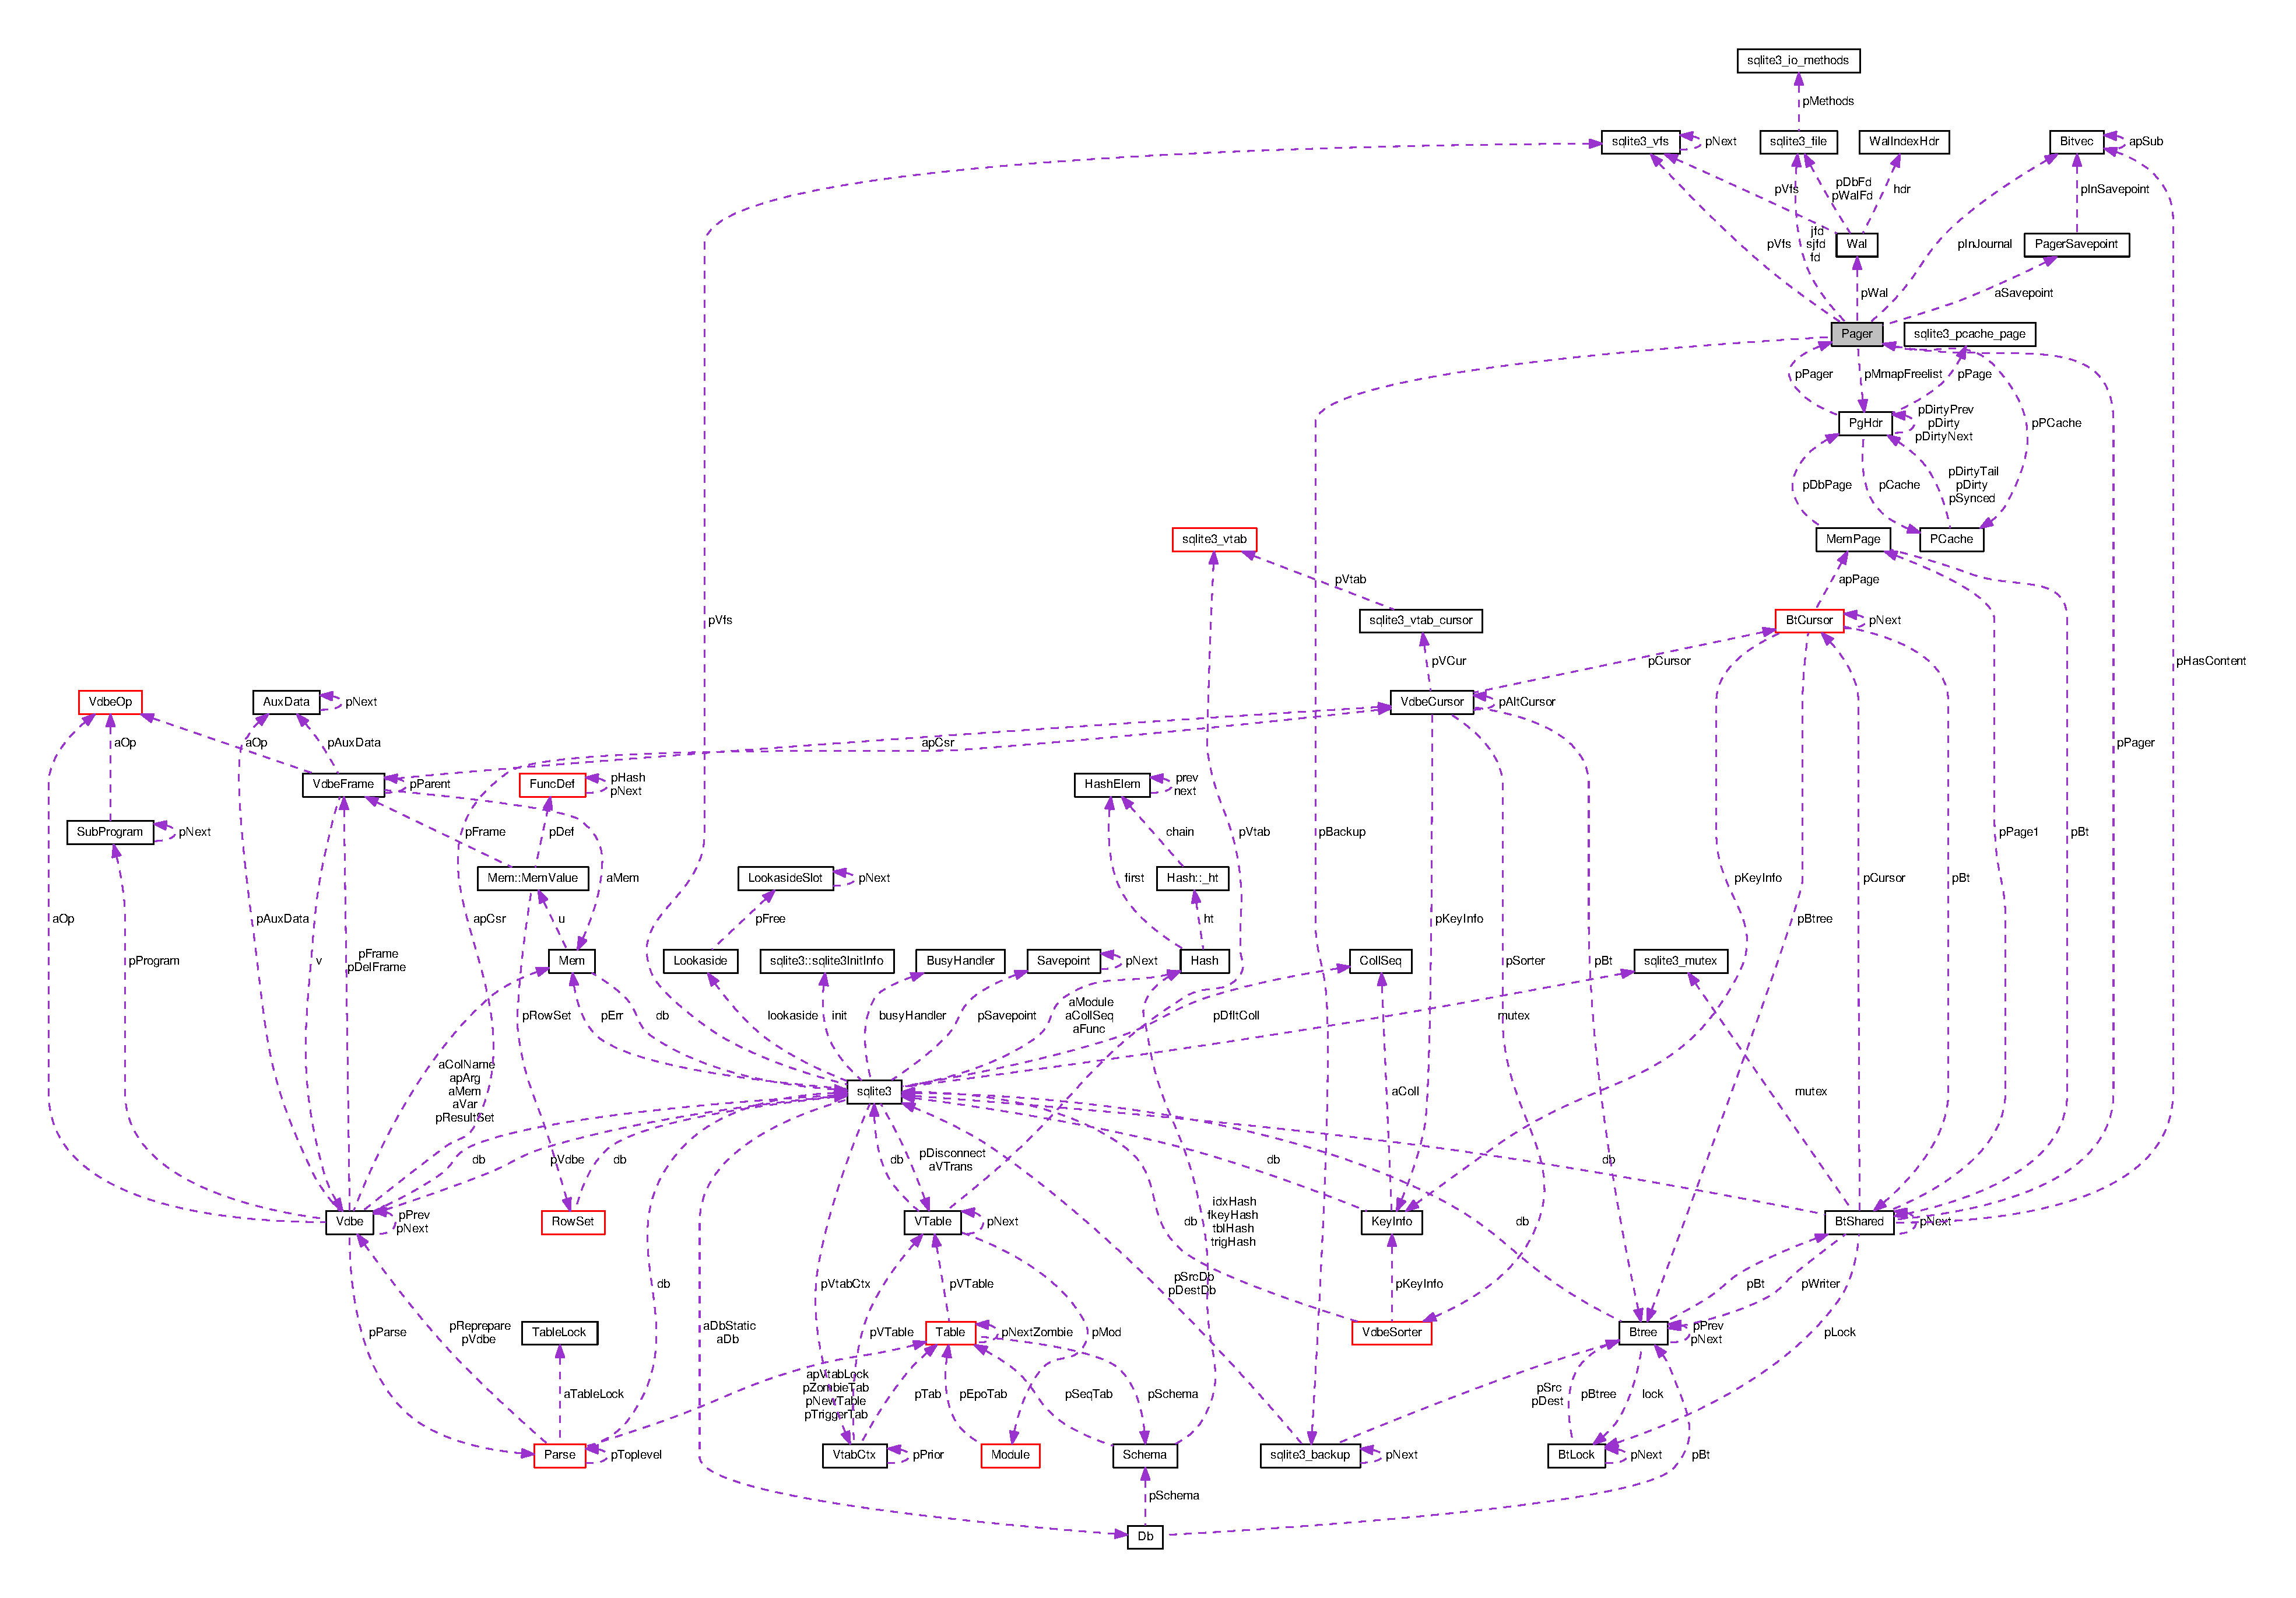
\includegraphics[width=350pt]{structPager__coll__graph}
\end{center}
\end{figure}
\subsection*{Public Attributes}
\begin{DoxyCompactItemize}
\item 
\hyperlink{structsqlite3__vfs}{sqlite3\+\_\+vfs} $\ast$ {\bfseries p\+Vfs}\hypertarget{structPager_affa78e08a7f691a4c8f7043e0b4c9212}{}\label{structPager_affa78e08a7f691a4c8f7043e0b4c9212}

\item 
u8 {\bfseries exclusive\+Mode}\hypertarget{structPager_a5cbccc156e07d6226cb65a7ab05ac116}{}\label{structPager_a5cbccc156e07d6226cb65a7ab05ac116}

\item 
u8 {\bfseries journal\+Mode}\hypertarget{structPager_a9ad7bd09f1c9323d943ee17ddf42e46e}{}\label{structPager_a9ad7bd09f1c9323d943ee17ddf42e46e}

\item 
u8 {\bfseries use\+Journal}\hypertarget{structPager_af7783f866150d7e322c28cb324ad85d6}{}\label{structPager_af7783f866150d7e322c28cb324ad85d6}

\item 
u8 {\bfseries no\+Sync}\hypertarget{structPager_ae943093a3ccbfbf264ccf3c8a52edac1}{}\label{structPager_ae943093a3ccbfbf264ccf3c8a52edac1}

\item 
u8 {\bfseries full\+Sync}\hypertarget{structPager_abae5c9c3d85120ae266acc4c9a355b86}{}\label{structPager_abae5c9c3d85120ae266acc4c9a355b86}

\item 
u8 {\bfseries extra\+Sync}\hypertarget{structPager_a942f1ff74fbe690c2777d181c791589f}{}\label{structPager_a942f1ff74fbe690c2777d181c791589f}

\item 
u8 {\bfseries ckpt\+Sync\+Flags}\hypertarget{structPager_a4543ec92953e7bda49b3ed4f0bdab890}{}\label{structPager_a4543ec92953e7bda49b3ed4f0bdab890}

\item 
u8 {\bfseries wal\+Sync\+Flags}\hypertarget{structPager_aa8c8c2d893e4d2165f089ddde3e85103}{}\label{structPager_aa8c8c2d893e4d2165f089ddde3e85103}

\item 
u8 {\bfseries sync\+Flags}\hypertarget{structPager_ac7f90d27da63090369a0e44a0bceb525}{}\label{structPager_ac7f90d27da63090369a0e44a0bceb525}

\item 
u8 {\bfseries temp\+File}\hypertarget{structPager_a9caa1abb43f6e839dd9a265c27b0b9e4}{}\label{structPager_a9caa1abb43f6e839dd9a265c27b0b9e4}

\item 
u8 {\bfseries no\+Lock}\hypertarget{structPager_a829f9ffd857c0959c1822e5301caf49f}{}\label{structPager_a829f9ffd857c0959c1822e5301caf49f}

\item 
u8 {\bfseries read\+Only}\hypertarget{structPager_ad7a7013309fd80a2a01844e69e8e7398}{}\label{structPager_ad7a7013309fd80a2a01844e69e8e7398}

\item 
u8 {\bfseries mem\+Db}\hypertarget{structPager_abca3633b7745075aa5cf432b3fae54f2}{}\label{structPager_abca3633b7745075aa5cf432b3fae54f2}

\item 
u8 {\bfseries e\+State}\hypertarget{structPager_af03ee0ac77cf73453295ffcf43e46b43}{}\label{structPager_af03ee0ac77cf73453295ffcf43e46b43}

\item 
u8 {\bfseries e\+Lock}\hypertarget{structPager_afcaf60e4b0be0995c926e3357d4bbef0}{}\label{structPager_afcaf60e4b0be0995c926e3357d4bbef0}

\item 
u8 {\bfseries change\+Count\+Done}\hypertarget{structPager_a90c86a51ec6805d5702d32e456b0bcdc}{}\label{structPager_a90c86a51ec6805d5702d32e456b0bcdc}

\item 
u8 {\bfseries set\+Master}\hypertarget{structPager_acd7eae0587c98ac41afab04e4b5defcb}{}\label{structPager_acd7eae0587c98ac41afab04e4b5defcb}

\item 
u8 {\bfseries do\+Not\+Spill}\hypertarget{structPager_a2f6579b3006b692a4ce1e5ad3e9a58ed}{}\label{structPager_a2f6579b3006b692a4ce1e5ad3e9a58ed}

\item 
u8 {\bfseries subj\+In\+Memory}\hypertarget{structPager_a9205654b516184d84fde5c3b5f72ff77}{}\label{structPager_a9205654b516184d84fde5c3b5f72ff77}

\item 
u8 {\bfseries b\+Use\+Fetch}\hypertarget{structPager_a35c15ace49e893cd5823222f549700e6}{}\label{structPager_a35c15ace49e893cd5823222f549700e6}

\item 
u8 {\bfseries has\+Held\+Shared\+Lock}\hypertarget{structPager_a8d4961bd8449f4bf8157763bb7e56b4f}{}\label{structPager_a8d4961bd8449f4bf8157763bb7e56b4f}

\item 
Pgno {\bfseries db\+Size}\hypertarget{structPager_afa5d7849190ef0a9a6f85bb15f2444b3}{}\label{structPager_afa5d7849190ef0a9a6f85bb15f2444b3}

\item 
Pgno {\bfseries db\+Orig\+Size}\hypertarget{structPager_a8f9cd11d6ae3fac48182e6eae0810c6a}{}\label{structPager_a8f9cd11d6ae3fac48182e6eae0810c6a}

\item 
Pgno {\bfseries db\+File\+Size}\hypertarget{structPager_a1f8f55f49cb0ec91bfde4dca96a13f13}{}\label{structPager_a1f8f55f49cb0ec91bfde4dca96a13f13}

\item 
Pgno {\bfseries db\+Hint\+Size}\hypertarget{structPager_aa99d74d10ef3cdcf61501f9777a0246b}{}\label{structPager_aa99d74d10ef3cdcf61501f9777a0246b}

\item 
int {\bfseries err\+Code}\hypertarget{structPager_addaf9648a1111d7b6c85166cf7c7a575}{}\label{structPager_addaf9648a1111d7b6c85166cf7c7a575}

\item 
int {\bfseries n\+Rec}\hypertarget{structPager_a3a202368c065a43695533503c98f28d9}{}\label{structPager_a3a202368c065a43695533503c98f28d9}

\item 
u32 {\bfseries cksum\+Init}\hypertarget{structPager_ad799667658328a44b471378a1b99623e}{}\label{structPager_ad799667658328a44b471378a1b99623e}

\item 
u32 {\bfseries n\+Sub\+Rec}\hypertarget{structPager_a670c4c54515c0257c35ddfc07c43763e}{}\label{structPager_a670c4c54515c0257c35ddfc07c43763e}

\item 
\hyperlink{structBitvec}{Bitvec} $\ast$ {\bfseries p\+In\+Journal}\hypertarget{structPager_a530ea868337a7c0c4e7c125035f73737}{}\label{structPager_a530ea868337a7c0c4e7c125035f73737}

\item 
\hyperlink{structsqlite3__file}{sqlite3\+\_\+file} $\ast$ {\bfseries fd}\hypertarget{structPager_a005ff1960fc1550a870cd1dae418c99e}{}\label{structPager_a005ff1960fc1550a870cd1dae418c99e}

\item 
\hyperlink{structsqlite3__file}{sqlite3\+\_\+file} $\ast$ {\bfseries jfd}\hypertarget{structPager_a81057c4420b8278e8141cf626abf4f0d}{}\label{structPager_a81057c4420b8278e8141cf626abf4f0d}

\item 
\hyperlink{structsqlite3__file}{sqlite3\+\_\+file} $\ast$ {\bfseries sjfd}\hypertarget{structPager_a8196bcc97f184d480848895f71e080e6}{}\label{structPager_a8196bcc97f184d480848895f71e080e6}

\item 
i64 {\bfseries journal\+Off}\hypertarget{structPager_ad3cffdc0987965fa6a472b19355f48df}{}\label{structPager_ad3cffdc0987965fa6a472b19355f48df}

\item 
i64 {\bfseries journal\+Hdr}\hypertarget{structPager_a7f4a7f5f0245b063a82c185f40bad7f0}{}\label{structPager_a7f4a7f5f0245b063a82c185f40bad7f0}

\item 
\hyperlink{structsqlite3__backup}{sqlite3\+\_\+backup} $\ast$ {\bfseries p\+Backup}\hypertarget{structPager_ae230d34da61bf28178fa1ac142a88c15}{}\label{structPager_ae230d34da61bf28178fa1ac142a88c15}

\item 
\hyperlink{structPagerSavepoint}{Pager\+Savepoint} $\ast$ {\bfseries a\+Savepoint}\hypertarget{structPager_a4d5f4487316c026eceb8461e90fffcfd}{}\label{structPager_a4d5f4487316c026eceb8461e90fffcfd}

\item 
int {\bfseries n\+Savepoint}\hypertarget{structPager_a020adae89ef6c1b28e51fffc3d4b22c9}{}\label{structPager_a020adae89ef6c1b28e51fffc3d4b22c9}

\item 
u32 {\bfseries i\+Data\+Version}\hypertarget{structPager_a4464625e1489082ddb9129b6b5db0583}{}\label{structPager_a4464625e1489082ddb9129b6b5db0583}

\item 
char {\bfseries db\+File\+Vers} \mbox{[}16\mbox{]}\hypertarget{structPager_acf03a47838eee1cf474bb93dbc834b5f}{}\label{structPager_acf03a47838eee1cf474bb93dbc834b5f}

\item 
int {\bfseries n\+Mmap\+Out}\hypertarget{structPager_acacf681e33935075e2b19e0906574b95}{}\label{structPager_acacf681e33935075e2b19e0906574b95}

\item 
sqlite3\+\_\+int64 {\bfseries sz\+Mmap}\hypertarget{structPager_a2e1c04a512708f6df091f6d6246b70d3}{}\label{structPager_a2e1c04a512708f6df091f6d6246b70d3}

\item 
\hyperlink{structPgHdr}{Pg\+Hdr} $\ast$ {\bfseries p\+Mmap\+Freelist}\hypertarget{structPager_a2213dad45ad7c79cf50dcdaf9bf6a718}{}\label{structPager_a2213dad45ad7c79cf50dcdaf9bf6a718}

\item 
u16 {\bfseries n\+Extra}\hypertarget{structPager_a44e153b2f756bfb86ab471c25893b3b6}{}\label{structPager_a44e153b2f756bfb86ab471c25893b3b6}

\item 
i16 {\bfseries n\+Reserve}\hypertarget{structPager_a82581087240713cab679108e3adeaf58}{}\label{structPager_a82581087240713cab679108e3adeaf58}

\item 
u32 {\bfseries vfs\+Flags}\hypertarget{structPager_a36f3333fe82c70a46a99f2f8f289a971}{}\label{structPager_a36f3333fe82c70a46a99f2f8f289a971}

\item 
u32 {\bfseries sector\+Size}\hypertarget{structPager_a4a47c73d7c18b803df33ba6c39baa5bf}{}\label{structPager_a4a47c73d7c18b803df33ba6c39baa5bf}

\item 
int {\bfseries page\+Size}\hypertarget{structPager_a9cfb910e7eaf8442f5414d722232a6e9}{}\label{structPager_a9cfb910e7eaf8442f5414d722232a6e9}

\item 
Pgno {\bfseries mx\+Pgno}\hypertarget{structPager_ad1d9a508ac764486a5eaef9b4f7781af}{}\label{structPager_ad1d9a508ac764486a5eaef9b4f7781af}

\item 
i64 {\bfseries journal\+Size\+Limit}\hypertarget{structPager_ae381db4e0b49f92596b0cdeb279e6bc6}{}\label{structPager_ae381db4e0b49f92596b0cdeb279e6bc6}

\item 
char $\ast$ {\bfseries z\+Filename}\hypertarget{structPager_a2a55a044468f8658b7993e57087a5561}{}\label{structPager_a2a55a044468f8658b7993e57087a5561}

\item 
char $\ast$ {\bfseries z\+Journal}\hypertarget{structPager_ab36ce1f606c407ad3fc56a3651f5a319}{}\label{structPager_ab36ce1f606c407ad3fc56a3651f5a319}

\item 
int($\ast$ {\bfseries x\+Busy\+Handler} )(void $\ast$)\hypertarget{structPager_ae1f5a3f57a0351a2d2f652716c48c463}{}\label{structPager_ae1f5a3f57a0351a2d2f652716c48c463}

\item 
void $\ast$ {\bfseries p\+Busy\+Handler\+Arg}\hypertarget{structPager_a7a685e7a8dcbcd725c5a982fd8deb91b}{}\label{structPager_a7a685e7a8dcbcd725c5a982fd8deb91b}

\item 
int {\bfseries a\+Stat} \mbox{[}3\mbox{]}\hypertarget{structPager_a0b3bb8afc7c4c82e0e99f3ad99dd0986}{}\label{structPager_a0b3bb8afc7c4c82e0e99f3ad99dd0986}

\item 
void($\ast$ {\bfseries x\+Reiniter} )(\hyperlink{structPgHdr}{Db\+Page} $\ast$)\hypertarget{structPager_ad214904b953afe7d4718a713fedb8c98}{}\label{structPager_ad214904b953afe7d4718a713fedb8c98}

\item 
char $\ast$ {\bfseries p\+Tmp\+Space}\hypertarget{structPager_a64934188c72599e0be9ae54d3fc1cc92}{}\label{structPager_a64934188c72599e0be9ae54d3fc1cc92}

\item 
\hyperlink{structPCache}{P\+Cache} $\ast$ {\bfseries p\+P\+Cache}\hypertarget{structPager_ae2495e45e354e92a858144386f91cab3}{}\label{structPager_ae2495e45e354e92a858144386f91cab3}

\item 
\hyperlink{structWal}{Wal} $\ast$ {\bfseries p\+Wal}\hypertarget{structPager_a2c759424108248d8b08e6f400fab14dd}{}\label{structPager_a2c759424108248d8b08e6f400fab14dd}

\item 
char $\ast$ {\bfseries z\+Wal}\hypertarget{structPager_ac63ab281e48f9ac8521b85c1a90475b3}{}\label{structPager_ac63ab281e48f9ac8521b85c1a90475b3}

\end{DoxyCompactItemize}


The documentation for this struct was generated from the following file\+:\begin{DoxyCompactItemize}
\item 
sqlite3.\+c\end{DoxyCompactItemize}

\hypertarget{structPagerSavepoint}{}\section{Pager\+Savepoint Struct Reference}
\label{structPagerSavepoint}\index{Pager\+Savepoint@{Pager\+Savepoint}}


Collaboration diagram for Pager\+Savepoint\+:
% FIG 0
\subsection*{Public Attributes}
\begin{DoxyCompactItemize}
\item 
i64 {\bfseries i\+Offset}\hypertarget{structPagerSavepoint_ab3ee7b75a10f47a82c8e3312bee6ad60}{}\label{structPagerSavepoint_ab3ee7b75a10f47a82c8e3312bee6ad60}

\item 
i64 {\bfseries i\+Hdr\+Offset}\hypertarget{structPagerSavepoint_ae1afd1cf4fba6f7efd232656366121d1}{}\label{structPagerSavepoint_ae1afd1cf4fba6f7efd232656366121d1}

\item 
\hyperlink{structBitvec}{Bitvec} $\ast$ {\bfseries p\+In\+Savepoint}\hypertarget{structPagerSavepoint_abf7d6dc9d457c866727f84c4b9e0348f}{}\label{structPagerSavepoint_abf7d6dc9d457c866727f84c4b9e0348f}

\item 
Pgno {\bfseries n\+Orig}\hypertarget{structPagerSavepoint_a944cca2844a51bdba253476f516b9865}{}\label{structPagerSavepoint_a944cca2844a51bdba253476f516b9865}

\item 
Pgno {\bfseries i\+Sub\+Rec}\hypertarget{structPagerSavepoint_ac1accce313b9da31631892e2cbe85a2f}{}\label{structPagerSavepoint_ac1accce313b9da31631892e2cbe85a2f}

\item 
u32 {\bfseries a\+Wal\+Data} \mbox{[}W\+A\+L\+\_\+\+S\+A\+V\+E\+P\+O\+I\+N\+T\+\_\+\+N\+D\+A\+TA\mbox{]}\hypertarget{structPagerSavepoint_ac96cff844a24378c426a9901517f1d6c}{}\label{structPagerSavepoint_ac96cff844a24378c426a9901517f1d6c}

\end{DoxyCompactItemize}


The documentation for this struct was generated from the following file\+:\begin{DoxyCompactItemize}
\item 
sqlite3.\+c\end{DoxyCompactItemize}

\hypertarget{structParse}{}\section{Parse Struct Reference}
\label{structParse}\index{Parse@{Parse}}


Collaboration diagram for Parse\+:\nopagebreak
\begin{figure}[H]
\begin{center}
\leavevmode
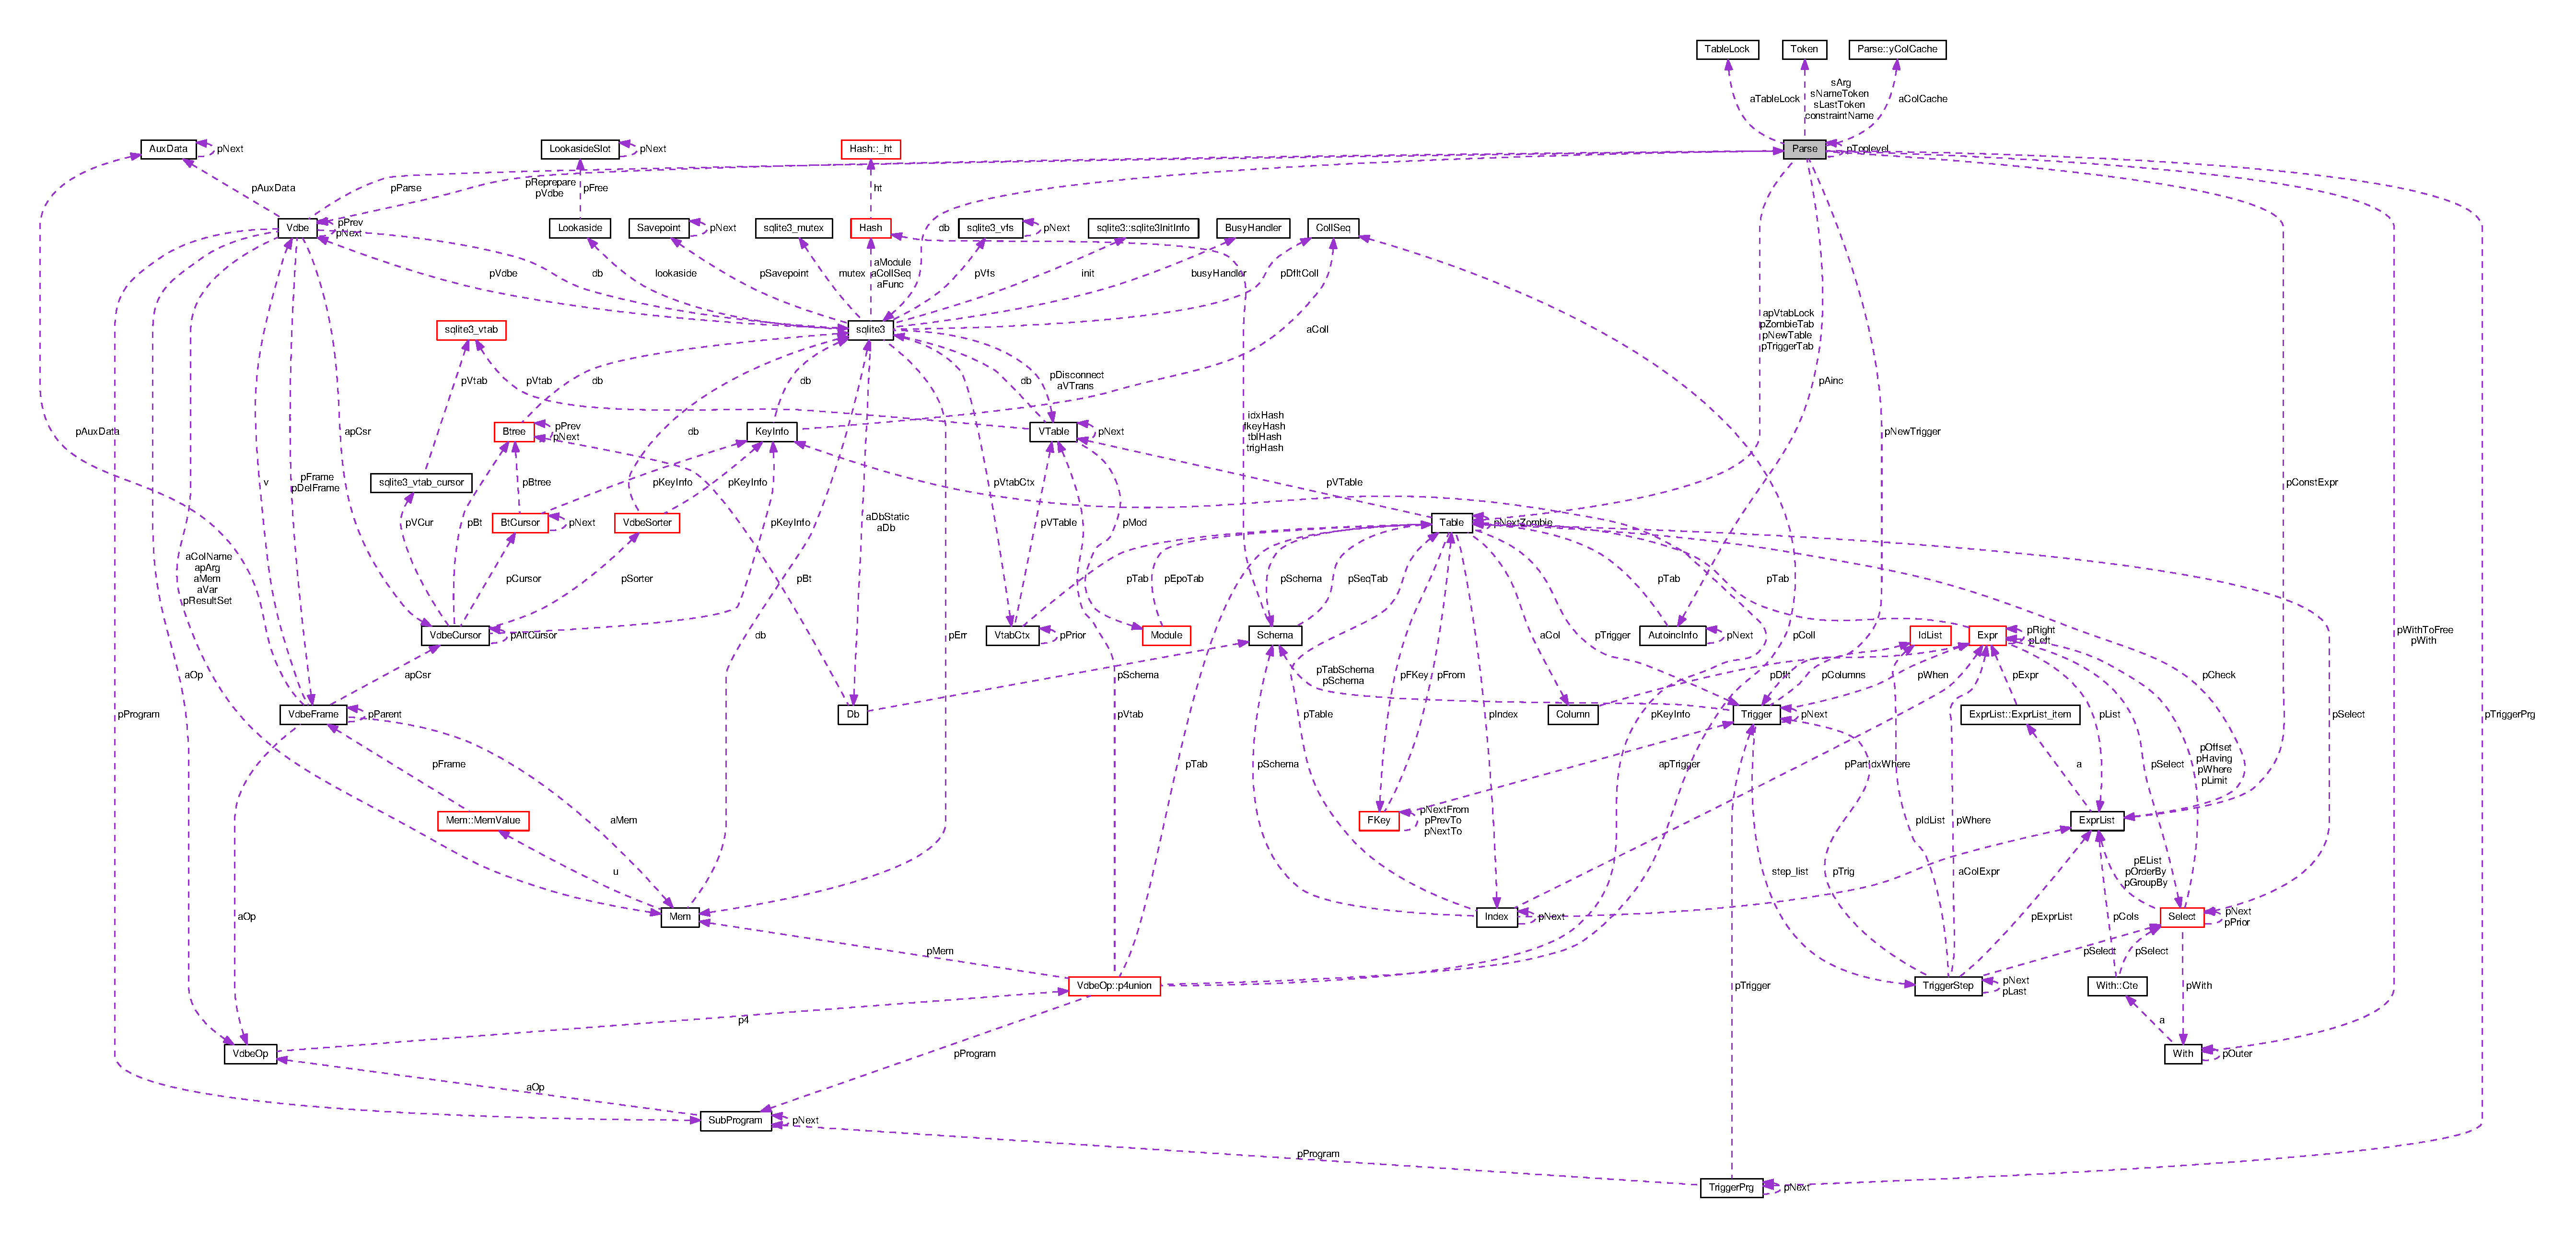
\includegraphics[width=350pt]{structParse__coll__graph}
\end{center}
\end{figure}
\subsection*{Classes}
\begin{DoxyCompactItemize}
\item 
struct \hyperlink{structParse_1_1yColCache}{y\+Col\+Cache}
\end{DoxyCompactItemize}
\subsection*{Public Attributes}
\begin{DoxyCompactItemize}
\item 
\hyperlink{structsqlite3}{sqlite3} $\ast$ {\bfseries db}\hypertarget{structParse_a44364e5e1197927f89864ec345bc5491}{}\label{structParse_a44364e5e1197927f89864ec345bc5491}

\item 
char $\ast$ {\bfseries z\+Err\+Msg}\hypertarget{structParse_a04146757986ff4654c7b321654896e81}{}\label{structParse_a04146757986ff4654c7b321654896e81}

\item 
\hyperlink{structVdbe}{Vdbe} $\ast$ {\bfseries p\+Vdbe}\hypertarget{structParse_a81774053fd5063046f532c07e3daa98b}{}\label{structParse_a81774053fd5063046f532c07e3daa98b}

\item 
int {\bfseries rc}\hypertarget{structParse_a897c2ea40a1065d49a134f18ca251637}{}\label{structParse_a897c2ea40a1065d49a134f18ca251637}

\item 
u8 {\bfseries col\+Names\+Set}\hypertarget{structParse_a4c71fde634168abc1e3e32c70704b1ac}{}\label{structParse_a4c71fde634168abc1e3e32c70704b1ac}

\item 
u8 {\bfseries check\+Schema}\hypertarget{structParse_a13b660ed90fc83565aa542a10549ec9f}{}\label{structParse_a13b660ed90fc83565aa542a10549ec9f}

\item 
u8 {\bfseries nested}\hypertarget{structParse_a33d62687b6d368acf94e954490358819}{}\label{structParse_a33d62687b6d368acf94e954490358819}

\item 
u8 {\bfseries n\+Temp\+Reg}\hypertarget{structParse_ae292001c732781b6b94d28ca303e1aa5}{}\label{structParse_ae292001c732781b6b94d28ca303e1aa5}

\item 
u8 {\bfseries is\+Multi\+Write}\hypertarget{structParse_a027d06007eab8e01b8930357f321344b}{}\label{structParse_a027d06007eab8e01b8930357f321344b}

\item 
u8 {\bfseries may\+Abort}\hypertarget{structParse_a1813c80797fcdba29e95813284619e57}{}\label{structParse_a1813c80797fcdba29e95813284619e57}

\item 
u8 {\bfseries has\+Compound}\hypertarget{structParse_a53c500179a70ea59816dea3f6fa04b96}{}\label{structParse_a53c500179a70ea59816dea3f6fa04b96}

\item 
u8 {\bfseries ok\+Const\+Factor}\hypertarget{structParse_ad9f3adb62af32e4fa5fe0c0d8621ae7b}{}\label{structParse_ad9f3adb62af32e4fa5fe0c0d8621ae7b}

\item 
u8 {\bfseries disable\+Lookaside}\hypertarget{structParse_a633c38a8e4512eb6415813636e2e97b4}{}\label{structParse_a633c38a8e4512eb6415813636e2e97b4}

\item 
u8 {\bfseries n\+Col\+Cache}\hypertarget{structParse_a23b721a6d1beab831c1b88ebbf30f57e}{}\label{structParse_a23b721a6d1beab831c1b88ebbf30f57e}

\item 
int {\bfseries n\+Range\+Reg}\hypertarget{structParse_ae32922d3d20171f4acc426714b497e6f}{}\label{structParse_ae32922d3d20171f4acc426714b497e6f}

\item 
int {\bfseries i\+Range\+Reg}\hypertarget{structParse_a715f56a596d5172926c20dd7f91600b6}{}\label{structParse_a715f56a596d5172926c20dd7f91600b6}

\item 
int {\bfseries n\+Err}\hypertarget{structParse_ac7206f0c7e580ab32b7dfb20950bb1c9}{}\label{structParse_ac7206f0c7e580ab32b7dfb20950bb1c9}

\item 
int {\bfseries n\+Tab}\hypertarget{structParse_a6b3a46e1f275962fa8808dddba20ba23}{}\label{structParse_a6b3a46e1f275962fa8808dddba20ba23}

\item 
int {\bfseries n\+Mem}\hypertarget{structParse_aa66b48b0ababc17403615c899cddec9c}{}\label{structParse_aa66b48b0ababc17403615c899cddec9c}

\item 
int {\bfseries n\+Op\+Alloc}\hypertarget{structParse_a84dadce444e15f0584fa2a35a4e5eadf}{}\label{structParse_a84dadce444e15f0584fa2a35a4e5eadf}

\item 
int {\bfseries sz\+Op\+Alloc}\hypertarget{structParse_af9d073fc2f41afbe5a2f1c580f2333c9}{}\label{structParse_af9d073fc2f41afbe5a2f1c580f2333c9}

\item 
int {\bfseries ck\+Base}\hypertarget{structParse_a07e8e916fb569a86acfa5f380afaaf77}{}\label{structParse_a07e8e916fb569a86acfa5f380afaaf77}

\item 
int {\bfseries i\+Self\+Tab}\hypertarget{structParse_a5858bb3d9d291446cb5c435aa0ce9dbc}{}\label{structParse_a5858bb3d9d291446cb5c435aa0ce9dbc}

\item 
int {\bfseries i\+Cache\+Level}\hypertarget{structParse_a5b06d03e7605a6f55369481c050ac0a8}{}\label{structParse_a5b06d03e7605a6f55369481c050ac0a8}

\item 
int {\bfseries i\+Cache\+Cnt}\hypertarget{structParse_ac4633493fd5f100fa823344be1c19d1e}{}\label{structParse_ac4633493fd5f100fa823344be1c19d1e}

\item 
int {\bfseries n\+Label}\hypertarget{structParse_ab1a2fa5eb16fefcff4f61b19a1468f7d}{}\label{structParse_ab1a2fa5eb16fefcff4f61b19a1468f7d}

\item 
int $\ast$ {\bfseries a\+Label}\hypertarget{structParse_a67e861822e4cec97b0e45ec16fac3250}{}\label{structParse_a67e861822e4cec97b0e45ec16fac3250}

\item 
\hyperlink{structExprList}{Expr\+List} $\ast$ {\bfseries p\+Const\+Expr}\hypertarget{structParse_ab908ea67b6ac078ee3836fb8bf243002}{}\label{structParse_ab908ea67b6ac078ee3836fb8bf243002}

\item 
\hyperlink{structToken}{Token} {\bfseries constraint\+Name}\hypertarget{structParse_a40cbce90eedbd57143416c8bc28fec46}{}\label{structParse_a40cbce90eedbd57143416c8bc28fec46}

\item 
y\+Db\+Mask {\bfseries write\+Mask}\hypertarget{structParse_a4939b6d4fd3f48731b58b8a6f51417cd}{}\label{structParse_a4939b6d4fd3f48731b58b8a6f51417cd}

\item 
y\+Db\+Mask {\bfseries cookie\+Mask}\hypertarget{structParse_a7c0b37cf797fd157234cb2e306cba2e4}{}\label{structParse_a7c0b37cf797fd157234cb2e306cba2e4}

\item 
int {\bfseries reg\+Rowid}\hypertarget{structParse_a63f71c268a7a77cb0df5619dd8ebbacd}{}\label{structParse_a63f71c268a7a77cb0df5619dd8ebbacd}

\item 
int {\bfseries reg\+Root}\hypertarget{structParse_afcf3d47e9424b79e6911cf366cb73bd4}{}\label{structParse_afcf3d47e9424b79e6911cf366cb73bd4}

\item 
int {\bfseries n\+Max\+Arg}\hypertarget{structParse_aab781bff62f93c0f9a7ca979a3b3a820}{}\label{structParse_aab781bff62f93c0f9a7ca979a3b3a820}

\item 
int {\bfseries n\+Table\+Lock}\hypertarget{structParse_a8c61b1b13dcb394b190fa09f5c253928}{}\label{structParse_a8c61b1b13dcb394b190fa09f5c253928}

\item 
\hyperlink{structTableLock}{Table\+Lock} $\ast$ {\bfseries a\+Table\+Lock}\hypertarget{structParse_ae8e553d660dc69d285945d3db8f127c7}{}\label{structParse_ae8e553d660dc69d285945d3db8f127c7}

\item 
\hyperlink{structAutoincInfo}{Autoinc\+Info} $\ast$ {\bfseries p\+Ainc}\hypertarget{structParse_a23de0e2b2dc60ac5f5932c5b2cd34f10}{}\label{structParse_a23de0e2b2dc60ac5f5932c5b2cd34f10}

\item 
\hyperlink{structParse}{Parse} $\ast$ {\bfseries p\+Toplevel}\hypertarget{structParse_a739df7b56510f22e64aba1ed203fec76}{}\label{structParse_a739df7b56510f22e64aba1ed203fec76}

\item 
\hyperlink{structTable}{Table} $\ast$ {\bfseries p\+Trigger\+Tab}\hypertarget{structParse_aad9b1145e39b240e842f9c2ad8e7e230}{}\label{structParse_aad9b1145e39b240e842f9c2ad8e7e230}

\item 
int {\bfseries addr\+Cr\+Tab}\hypertarget{structParse_a4ca16d26d451cd965dbb81906f9c6b0e}{}\label{structParse_a4ca16d26d451cd965dbb81906f9c6b0e}

\item 
u32 {\bfseries n\+Query\+Loop}\hypertarget{structParse_ae85aa19104aeeab3cc7241bfd8b5d553}{}\label{structParse_ae85aa19104aeeab3cc7241bfd8b5d553}

\item 
u32 {\bfseries oldmask}\hypertarget{structParse_acda3334b932ac6541f45fa939053e942}{}\label{structParse_acda3334b932ac6541f45fa939053e942}

\item 
u32 {\bfseries newmask}\hypertarget{structParse_a698d9e9d4938cc35a4ef9137a46f1840}{}\label{structParse_a698d9e9d4938cc35a4ef9137a46f1840}

\item 
u8 {\bfseries e\+Trigger\+Op}\hypertarget{structParse_addd3028173ab100a8802dfcc9b13ffb7}{}\label{structParse_addd3028173ab100a8802dfcc9b13ffb7}

\item 
u8 {\bfseries e\+Orconf}\hypertarget{structParse_a67083fd2286b7d5276831e84a1a16680}{}\label{structParse_a67083fd2286b7d5276831e84a1a16680}

\item 
u8 {\bfseries disable\+Triggers}\hypertarget{structParse_a5ea9b658f4cfacf4b35f18c51e144ef1}{}\label{structParse_a5ea9b658f4cfacf4b35f18c51e144ef1}

\item 
struct \hyperlink{structParse_1_1yColCache}{Parse\+::y\+Col\+Cache} {\bfseries a\+Col\+Cache} \mbox{[}S\+Q\+L\+I\+T\+E\+\_\+\+N\+\_\+\+C\+O\+L\+C\+A\+C\+HE\mbox{]}\hypertarget{structParse_a788b85979d58b84e06bc367bac5b3f3f}{}\label{structParse_a788b85979d58b84e06bc367bac5b3f3f}

\item 
int {\bfseries a\+Temp\+Reg} \mbox{[}8\mbox{]}\hypertarget{structParse_ae2bd2e74d0caaab7a741d17b62f01ebc}{}\label{structParse_ae2bd2e74d0caaab7a741d17b62f01ebc}

\item 
\hyperlink{structToken}{Token} {\bfseries s\+Name\+Token}\hypertarget{structParse_afd929c54566cfc4d6f748fcc6b79b973}{}\label{structParse_afd929c54566cfc4d6f748fcc6b79b973}

\item 
\hyperlink{structToken}{Token} {\bfseries s\+Last\+Token}\hypertarget{structParse_ad499020d1bf06f3c98c8d36e2ceb83fd}{}\label{structParse_ad499020d1bf06f3c98c8d36e2ceb83fd}

\item 
yn\+Var {\bfseries n\+Var}\hypertarget{structParse_ae529f84d792c36e3f474e2ff89f0b6e4}{}\label{structParse_ae529f84d792c36e3f474e2ff89f0b6e4}

\item 
int {\bfseries nz\+Var}\hypertarget{structParse_ac9cf894d9dfd0ba37d9467cd9d2e48f0}{}\label{structParse_ac9cf894d9dfd0ba37d9467cd9d2e48f0}

\item 
u8 {\bfseries i\+Pk\+Sort\+Order}\hypertarget{structParse_a2be71f432ab79d2db44f1fcbbce55488}{}\label{structParse_a2be71f432ab79d2db44f1fcbbce55488}

\item 
u8 {\bfseries explain}\hypertarget{structParse_a41f7ea55f0d6523295a5d958e25a2787}{}\label{structParse_a41f7ea55f0d6523295a5d958e25a2787}

\item 
u8 {\bfseries declare\+Vtab}\hypertarget{structParse_a86c869df65cd788025680de9b6a9b1f1}{}\label{structParse_a86c869df65cd788025680de9b6a9b1f1}

\item 
int {\bfseries n\+Vtab\+Lock}\hypertarget{structParse_a7db8fe1ce2f0ec6bda7dc729a0e6a6e3}{}\label{structParse_a7db8fe1ce2f0ec6bda7dc729a0e6a6e3}

\item 
int {\bfseries n\+Height}\hypertarget{structParse_af4ec053d44a2a3bc8ae82b69a7327c3c}{}\label{structParse_af4ec053d44a2a3bc8ae82b69a7327c3c}

\item 
int {\bfseries i\+Select\+Id}\hypertarget{structParse_a7474fa0bf9ad160cbdf723406c306d9d}{}\label{structParse_a7474fa0bf9ad160cbdf723406c306d9d}

\item 
int {\bfseries i\+Next\+Select\+Id}\hypertarget{structParse_aab76240bd43c005941431179d4f9bf49}{}\label{structParse_aab76240bd43c005941431179d4f9bf49}

\item 
char $\ast$$\ast$ {\bfseries az\+Var}\hypertarget{structParse_a907e389eb399f3e76a0cc6b469e4e252}{}\label{structParse_a907e389eb399f3e76a0cc6b469e4e252}

\item 
\hyperlink{structVdbe}{Vdbe} $\ast$ {\bfseries p\+Reprepare}\hypertarget{structParse_a5e250f77353fb3df6660ff29ffa53790}{}\label{structParse_a5e250f77353fb3df6660ff29ffa53790}

\item 
const char $\ast$ {\bfseries z\+Tail}\hypertarget{structParse_a14f58728b3ae2a297272510ae4bd9a89}{}\label{structParse_a14f58728b3ae2a297272510ae4bd9a89}

\item 
\hyperlink{structTable}{Table} $\ast$ {\bfseries p\+New\+Table}\hypertarget{structParse_a4788769c077dc86ffa3ee1e40ed6b4a1}{}\label{structParse_a4788769c077dc86ffa3ee1e40ed6b4a1}

\item 
\hyperlink{structTrigger}{Trigger} $\ast$ {\bfseries p\+New\+Trigger}\hypertarget{structParse_a92ea8f2ac3190dd7c8360e0334ae78b3}{}\label{structParse_a92ea8f2ac3190dd7c8360e0334ae78b3}

\item 
const char $\ast$ {\bfseries z\+Auth\+Context}\hypertarget{structParse_a12c6e2fb69848bcc57169d44993c351f}{}\label{structParse_a12c6e2fb69848bcc57169d44993c351f}

\item 
\hyperlink{structToken}{Token} {\bfseries s\+Arg}\hypertarget{structParse_aa3fe38b31dd1cd0fbea4de0e77891642}{}\label{structParse_aa3fe38b31dd1cd0fbea4de0e77891642}

\item 
\hyperlink{structTable}{Table} $\ast$$\ast$ {\bfseries ap\+Vtab\+Lock}\hypertarget{structParse_acdfd318c0f04ec640d6affc85ef8a009}{}\label{structParse_acdfd318c0f04ec640d6affc85ef8a009}

\item 
\hyperlink{structTable}{Table} $\ast$ {\bfseries p\+Zombie\+Tab}\hypertarget{structParse_a4e8319f0a7f0d21e472c13ac6cf67060}{}\label{structParse_a4e8319f0a7f0d21e472c13ac6cf67060}

\item 
\hyperlink{structTriggerPrg}{Trigger\+Prg} $\ast$ {\bfseries p\+Trigger\+Prg}\hypertarget{structParse_a0891dbd3b583594c5d07d7b061026ea4}{}\label{structParse_a0891dbd3b583594c5d07d7b061026ea4}

\item 
\hyperlink{structWith}{With} $\ast$ {\bfseries p\+With}\hypertarget{structParse_a7a812b036ddcc4b838b956328e1ff03e}{}\label{structParse_a7a812b036ddcc4b838b956328e1ff03e}

\item 
\hyperlink{structWith}{With} $\ast$ {\bfseries p\+With\+To\+Free}\hypertarget{structParse_ae8e4463fa9d87da2833a542e27dd722d}{}\label{structParse_ae8e4463fa9d87da2833a542e27dd722d}

\end{DoxyCompactItemize}


The documentation for this struct was generated from the following file\+:\begin{DoxyCompactItemize}
\item 
sqlite3.\+c\end{DoxyCompactItemize}

\hypertarget{structPCache}{}\section{P\+Cache Struct Reference}
\label{structPCache}\index{P\+Cache@{P\+Cache}}


Collaboration diagram for P\+Cache\+:
% FIG 0
\subsection*{Public Attributes}
\begin{DoxyCompactItemize}
\item 
\hyperlink{structPgHdr}{Pg\+Hdr} $\ast$ {\bfseries p\+Dirty}\hypertarget{structPCache_a1c692ce92c7d3fc7c6c1324d5658b252}{}\label{structPCache_a1c692ce92c7d3fc7c6c1324d5658b252}

\item 
\hyperlink{structPgHdr}{Pg\+Hdr} $\ast$ {\bfseries p\+Dirty\+Tail}\hypertarget{structPCache_a8eaca309bfb8fa49e7c5e77dd3398bb0}{}\label{structPCache_a8eaca309bfb8fa49e7c5e77dd3398bb0}

\item 
\hyperlink{structPgHdr}{Pg\+Hdr} $\ast$ {\bfseries p\+Synced}\hypertarget{structPCache_a607eabd6768dd8df47d8fa353542b106}{}\label{structPCache_a607eabd6768dd8df47d8fa353542b106}

\item 
int {\bfseries n\+Ref\+Sum}\hypertarget{structPCache_a9688476c9cab5a7af8d09860567759eb}{}\label{structPCache_a9688476c9cab5a7af8d09860567759eb}

\item 
int {\bfseries sz\+Cache}\hypertarget{structPCache_a93ed4b9d731d883c3ed22a5adfd9c636}{}\label{structPCache_a93ed4b9d731d883c3ed22a5adfd9c636}

\item 
int {\bfseries sz\+Spill}\hypertarget{structPCache_abd30c4610f4087dad64f75e6c4e1e332}{}\label{structPCache_abd30c4610f4087dad64f75e6c4e1e332}

\item 
int {\bfseries sz\+Page}\hypertarget{structPCache_abb0bd0a3292780dcc07cb59bc577990d}{}\label{structPCache_abb0bd0a3292780dcc07cb59bc577990d}

\item 
int {\bfseries sz\+Extra}\hypertarget{structPCache_abcb37fcd3ea098b98a196a3f69e3c135}{}\label{structPCache_abcb37fcd3ea098b98a196a3f69e3c135}

\item 
u8 {\bfseries b\+Purgeable}\hypertarget{structPCache_a87ff1d0738734375524e544cefa33b01}{}\label{structPCache_a87ff1d0738734375524e544cefa33b01}

\item 
u8 {\bfseries e\+Create}\hypertarget{structPCache_a28629953493154d29ab7b6485a0471bf}{}\label{structPCache_a28629953493154d29ab7b6485a0471bf}

\item 
int($\ast$ {\bfseries x\+Stress} )(void $\ast$, \hyperlink{structPgHdr}{Pg\+Hdr} $\ast$)\hypertarget{structPCache_a51b67ce6c17cbd7124c50d8a2d0fed50}{}\label{structPCache_a51b67ce6c17cbd7124c50d8a2d0fed50}

\item 
void $\ast$ {\bfseries p\+Stress}\hypertarget{structPCache_af04a2ea8a2c6d6b3eea7bb7051b8f447}{}\label{structPCache_af04a2ea8a2c6d6b3eea7bb7051b8f447}

\item 
sqlite3\+\_\+pcache $\ast$ {\bfseries p\+Cache}\hypertarget{structPCache_ad0248655d30d327e0eeced6c3651b161}{}\label{structPCache_ad0248655d30d327e0eeced6c3651b161}

\end{DoxyCompactItemize}


The documentation for this struct was generated from the following file\+:\begin{DoxyCompactItemize}
\item 
sqlite3.\+c\end{DoxyCompactItemize}

\hypertarget{structPCache1}{}\section{P\+Cache1 Struct Reference}
\label{structPCache1}\index{P\+Cache1@{P\+Cache1}}


Collaboration diagram for P\+Cache1\+:
% FIG 0
\subsection*{Public Attributes}
\begin{DoxyCompactItemize}
\item 
\hyperlink{structPGroup}{P\+Group} $\ast$ {\bfseries p\+Group}\hypertarget{structPCache1_ae3389f0c68d6946a1eebeeee835ece69}{}\label{structPCache1_ae3389f0c68d6946a1eebeeee835ece69}

\item 
int {\bfseries sz\+Page}\hypertarget{structPCache1_a1425039a858b7518c097d8ae92597de0}{}\label{structPCache1_a1425039a858b7518c097d8ae92597de0}

\item 
int {\bfseries sz\+Extra}\hypertarget{structPCache1_a1e96e6671732e0af641732991b681ede}{}\label{structPCache1_a1e96e6671732e0af641732991b681ede}

\item 
int {\bfseries sz\+Alloc}\hypertarget{structPCache1_aa40b14da40f3c940978af20e99500000}{}\label{structPCache1_aa40b14da40f3c940978af20e99500000}

\item 
int {\bfseries b\+Purgeable}\hypertarget{structPCache1_a2af7d24e27369252addec9bef45afcfc}{}\label{structPCache1_a2af7d24e27369252addec9bef45afcfc}

\item 
unsigned int {\bfseries n\+Min}\hypertarget{structPCache1_a9e96c79ec60c2e368f92a2ba52d01c44}{}\label{structPCache1_a9e96c79ec60c2e368f92a2ba52d01c44}

\item 
unsigned int {\bfseries n\+Max}\hypertarget{structPCache1_aef08139a0b86b0c0a7ee2bec0bab2405}{}\label{structPCache1_aef08139a0b86b0c0a7ee2bec0bab2405}

\item 
unsigned int {\bfseries n90pct}\hypertarget{structPCache1_a8a5c5ab7d71e66c2a4df3f22513888f0}{}\label{structPCache1_a8a5c5ab7d71e66c2a4df3f22513888f0}

\item 
unsigned int {\bfseries i\+Max\+Key}\hypertarget{structPCache1_a2dff616ad2d1873ad3a8d20d53bcb4d0}{}\label{structPCache1_a2dff616ad2d1873ad3a8d20d53bcb4d0}

\item 
unsigned int {\bfseries n\+Recyclable}\hypertarget{structPCache1_a3501394bd251f08d1f9d26d3b2d4c67c}{}\label{structPCache1_a3501394bd251f08d1f9d26d3b2d4c67c}

\item 
unsigned int {\bfseries n\+Page}\hypertarget{structPCache1_ace332c276e28352992529f60f0ac457c}{}\label{structPCache1_ace332c276e28352992529f60f0ac457c}

\item 
unsigned int {\bfseries n\+Hash}\hypertarget{structPCache1_a09d9488a8a3a52822e33dd43e14c69e1}{}\label{structPCache1_a09d9488a8a3a52822e33dd43e14c69e1}

\item 
\hyperlink{structPgHdr1}{Pg\+Hdr1} $\ast$$\ast$ {\bfseries ap\+Hash}\hypertarget{structPCache1_a1169ec7ba2a628d89841d16ced651e1f}{}\label{structPCache1_a1169ec7ba2a628d89841d16ced651e1f}

\item 
\hyperlink{structPgHdr1}{Pg\+Hdr1} $\ast$ {\bfseries p\+Free}\hypertarget{structPCache1_a91dcc2d2771fa17cf065a1f9ff427d5f}{}\label{structPCache1_a91dcc2d2771fa17cf065a1f9ff427d5f}

\item 
void $\ast$ {\bfseries p\+Bulk}\hypertarget{structPCache1_a32591cc3f60587a1422627a080109fb7}{}\label{structPCache1_a32591cc3f60587a1422627a080109fb7}

\end{DoxyCompactItemize}


The documentation for this struct was generated from the following file\+:\begin{DoxyCompactItemize}
\item 
sqlite3.\+c\end{DoxyCompactItemize}

\hypertarget{structPgFreeslot}{}\section{Pg\+Freeslot Struct Reference}
\label{structPgFreeslot}\index{Pg\+Freeslot@{Pg\+Freeslot}}


Collaboration diagram for Pg\+Freeslot\+:\nopagebreak
\begin{figure}[H]
\begin{center}
\leavevmode
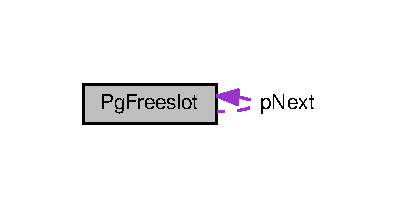
\includegraphics[width=192pt]{structPgFreeslot__coll__graph}
\end{center}
\end{figure}
\subsection*{Public Attributes}
\begin{DoxyCompactItemize}
\item 
\hyperlink{structPgFreeslot}{Pg\+Freeslot} $\ast$ {\bfseries p\+Next}\hypertarget{structPgFreeslot_ac38a6e51f86c650fb943585d7b6c8b70}{}\label{structPgFreeslot_ac38a6e51f86c650fb943585d7b6c8b70}

\end{DoxyCompactItemize}


The documentation for this struct was generated from the following file\+:\begin{DoxyCompactItemize}
\item 
sqlite3.\+c\end{DoxyCompactItemize}

\hypertarget{structPgHdr}{}\section{Pg\+Hdr Struct Reference}
\label{structPgHdr}\index{Pg\+Hdr@{Pg\+Hdr}}


Collaboration diagram for Pg\+Hdr\+:\nopagebreak
\begin{figure}[H]
\begin{center}
\leavevmode
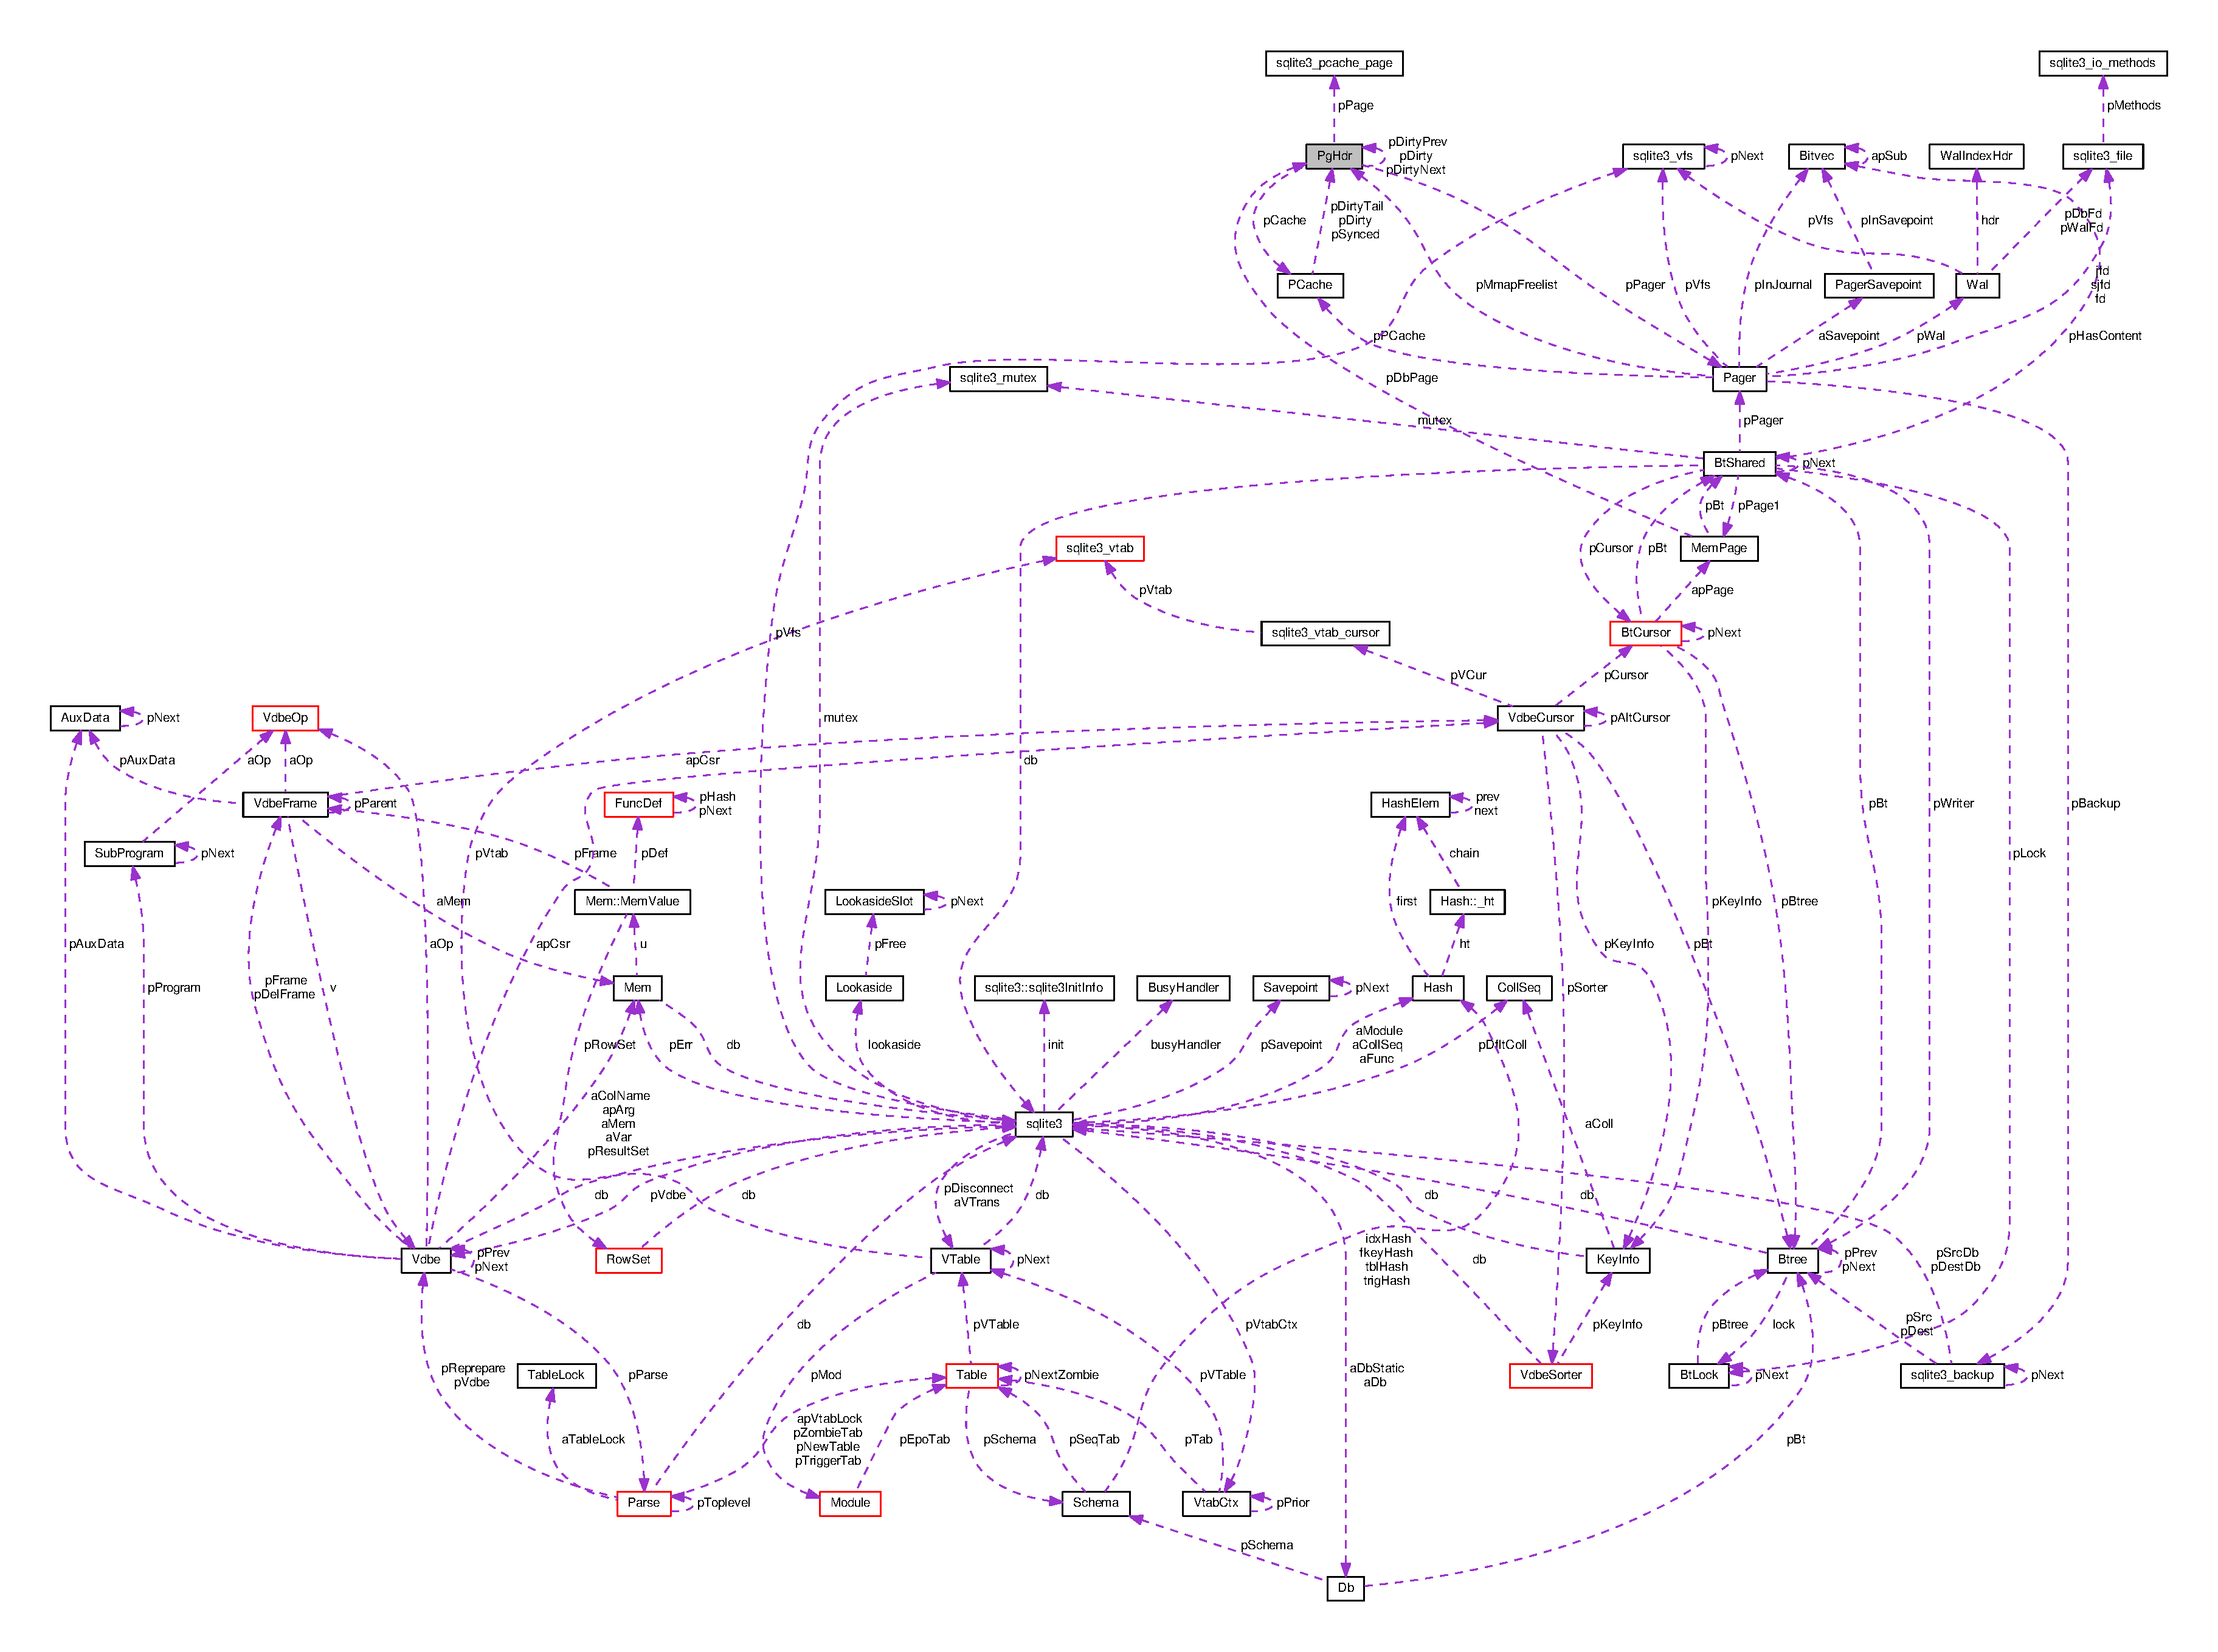
\includegraphics[width=350pt]{structPgHdr__coll__graph}
\end{center}
\end{figure}
\subsection*{Public Attributes}
\begin{DoxyCompactItemize}
\item 
\hyperlink{structsqlite3__pcache__page}{sqlite3\+\_\+pcache\+\_\+page} $\ast$ {\bfseries p\+Page}\hypertarget{structPgHdr_aa5645976ba0634993a7304dce8856c8b}{}\label{structPgHdr_aa5645976ba0634993a7304dce8856c8b}

\item 
void $\ast$ {\bfseries p\+Data}\hypertarget{structPgHdr_a0f9f2ac8492c0cdad5898036db20b798}{}\label{structPgHdr_a0f9f2ac8492c0cdad5898036db20b798}

\item 
void $\ast$ {\bfseries p\+Extra}\hypertarget{structPgHdr_a8ff7430ed04077f1ae20d10801968164}{}\label{structPgHdr_a8ff7430ed04077f1ae20d10801968164}

\item 
\hyperlink{structPgHdr}{Pg\+Hdr} $\ast$ {\bfseries p\+Dirty}\hypertarget{structPgHdr_a7732b1c0f19d9555ac93d4879fc95bbd}{}\label{structPgHdr_a7732b1c0f19d9555ac93d4879fc95bbd}

\item 
\hyperlink{structPager}{Pager} $\ast$ {\bfseries p\+Pager}\hypertarget{structPgHdr_aaa4879a9510c8a819a1e10a8ee21495b}{}\label{structPgHdr_aaa4879a9510c8a819a1e10a8ee21495b}

\item 
Pgno {\bfseries pgno}\hypertarget{structPgHdr_ab6e2223e410acf9bae7f12f1b1293589}{}\label{structPgHdr_ab6e2223e410acf9bae7f12f1b1293589}

\item 
u16 {\bfseries flags}\hypertarget{structPgHdr_a8ef58380f7e04f1e3c76fa208e227f95}{}\label{structPgHdr_a8ef58380f7e04f1e3c76fa208e227f95}

\item 
i16 {\bfseries n\+Ref}\hypertarget{structPgHdr_ac68c685d117788c18849e8853dd419d5}{}\label{structPgHdr_ac68c685d117788c18849e8853dd419d5}

\item 
\hyperlink{structPCache}{P\+Cache} $\ast$ {\bfseries p\+Cache}\hypertarget{structPgHdr_a557aeaddd1b0805815ce06f1bfd27782}{}\label{structPgHdr_a557aeaddd1b0805815ce06f1bfd27782}

\item 
\hyperlink{structPgHdr}{Pg\+Hdr} $\ast$ {\bfseries p\+Dirty\+Next}\hypertarget{structPgHdr_a61b56eb694ce445799963f7eb912e367}{}\label{structPgHdr_a61b56eb694ce445799963f7eb912e367}

\item 
\hyperlink{structPgHdr}{Pg\+Hdr} $\ast$ {\bfseries p\+Dirty\+Prev}\hypertarget{structPgHdr_a8392b45bb05d88c734020beb912304dc}{}\label{structPgHdr_a8392b45bb05d88c734020beb912304dc}

\end{DoxyCompactItemize}


The documentation for this struct was generated from the following file\+:\begin{DoxyCompactItemize}
\item 
sqlite3.\+c\end{DoxyCompactItemize}

\hypertarget{structPgHdr1}{}\section{Pg\+Hdr1 Struct Reference}
\label{structPgHdr1}\index{Pg\+Hdr1@{Pg\+Hdr1}}


Collaboration diagram for Pg\+Hdr1\+:\nopagebreak
\begin{figure}[H]
\begin{center}
\leavevmode
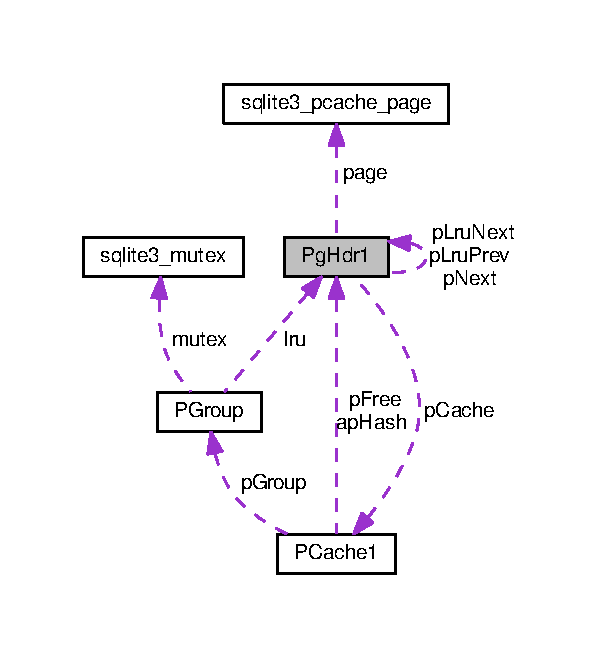
\includegraphics[width=288pt]{structPgHdr1__coll__graph}
\end{center}
\end{figure}
\subsection*{Public Attributes}
\begin{DoxyCompactItemize}
\item 
\hyperlink{structsqlite3__pcache__page}{sqlite3\+\_\+pcache\+\_\+page} {\bfseries page}\hypertarget{structPgHdr1_a121a9abbfea6b112ba77eeb84391ed47}{}\label{structPgHdr1_a121a9abbfea6b112ba77eeb84391ed47}

\item 
unsigned int {\bfseries i\+Key}\hypertarget{structPgHdr1_ad122ef74f5f0137414882aabd111a01b}{}\label{structPgHdr1_ad122ef74f5f0137414882aabd111a01b}

\item 
u8 {\bfseries is\+Pinned}\hypertarget{structPgHdr1_a361946b03e1d4664476d9ea3fce490d9}{}\label{structPgHdr1_a361946b03e1d4664476d9ea3fce490d9}

\item 
u8 {\bfseries is\+Bulk\+Local}\hypertarget{structPgHdr1_a1c07bb6fab410b7c9f41b24c44a118de}{}\label{structPgHdr1_a1c07bb6fab410b7c9f41b24c44a118de}

\item 
u8 {\bfseries is\+Anchor}\hypertarget{structPgHdr1_a232f677ac68bc8fbb7685e8a1955c810}{}\label{structPgHdr1_a232f677ac68bc8fbb7685e8a1955c810}

\item 
\hyperlink{structPgHdr1}{Pg\+Hdr1} $\ast$ {\bfseries p\+Next}\hypertarget{structPgHdr1_acde43ab0ed0fbba33e526058d9c343b9}{}\label{structPgHdr1_acde43ab0ed0fbba33e526058d9c343b9}

\item 
\hyperlink{structPCache1}{P\+Cache1} $\ast$ {\bfseries p\+Cache}\hypertarget{structPgHdr1_aa5b23de466773e72e1b6edf07b3a4570}{}\label{structPgHdr1_aa5b23de466773e72e1b6edf07b3a4570}

\item 
\hyperlink{structPgHdr1}{Pg\+Hdr1} $\ast$ {\bfseries p\+Lru\+Next}\hypertarget{structPgHdr1_ae22cfc3a39fe029a8f8fdd70e7ca4055}{}\label{structPgHdr1_ae22cfc3a39fe029a8f8fdd70e7ca4055}

\item 
\hyperlink{structPgHdr1}{Pg\+Hdr1} $\ast$ {\bfseries p\+Lru\+Prev}\hypertarget{structPgHdr1_adf220ef63d6ceb782ac87a08aeb1722d}{}\label{structPgHdr1_adf220ef63d6ceb782ac87a08aeb1722d}

\end{DoxyCompactItemize}


The documentation for this struct was generated from the following file\+:\begin{DoxyCompactItemize}
\item 
sqlite3.\+c\end{DoxyCompactItemize}

\hypertarget{structPGroup}{}\section{P\+Group Struct Reference}
\label{structPGroup}\index{P\+Group@{P\+Group}}


Collaboration diagram for P\+Group\+:\nopagebreak
\begin{figure}[H]
\begin{center}
\leavevmode
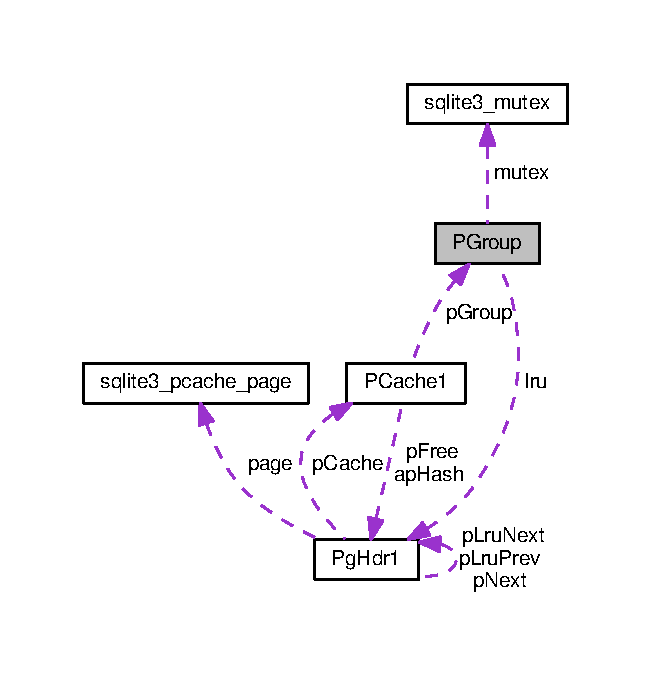
\includegraphics[width=313pt]{structPGroup__coll__graph}
\end{center}
\end{figure}
\subsection*{Public Attributes}
\begin{DoxyCompactItemize}
\item 
\hyperlink{structsqlite3__mutex}{sqlite3\+\_\+mutex} $\ast$ {\bfseries mutex}\hypertarget{structPGroup_a7173aa723aa61d6b1f79cde2f7d0f74d}{}\label{structPGroup_a7173aa723aa61d6b1f79cde2f7d0f74d}

\item 
unsigned int {\bfseries n\+Max\+Page}\hypertarget{structPGroup_a219ff89d38529cbb6b47e60f41896f41}{}\label{structPGroup_a219ff89d38529cbb6b47e60f41896f41}

\item 
unsigned int {\bfseries n\+Min\+Page}\hypertarget{structPGroup_aedf84324cb7138c9f9ee31814e8274c0}{}\label{structPGroup_aedf84324cb7138c9f9ee31814e8274c0}

\item 
unsigned int {\bfseries mx\+Pinned}\hypertarget{structPGroup_ac7cdffac1c20d260e8230dba4ab05cea}{}\label{structPGroup_ac7cdffac1c20d260e8230dba4ab05cea}

\item 
unsigned int {\bfseries n\+Current\+Page}\hypertarget{structPGroup_a532a09e3e6bf7a20a934764b4bd698a5}{}\label{structPGroup_a532a09e3e6bf7a20a934764b4bd698a5}

\item 
\hyperlink{structPgHdr1}{Pg\+Hdr1} {\bfseries lru}\hypertarget{structPGroup_a73c1201996cb4750677fdf1d73f50a92}{}\label{structPGroup_a73c1201996cb4750677fdf1d73f50a92}

\end{DoxyCompactItemize}


The documentation for this struct was generated from the following file\+:\begin{DoxyCompactItemize}
\item 
sqlite3.\+c\end{DoxyCompactItemize}

\hypertarget{structPmaReader}{}\section{Pma\+Reader Struct Reference}
\label{structPmaReader}\index{Pma\+Reader@{Pma\+Reader}}


Collaboration diagram for Pma\+Reader\+:
% FIG 0
\subsection*{Public Attributes}
\begin{DoxyCompactItemize}
\item 
i64 {\bfseries i\+Read\+Off}\hypertarget{structPmaReader_a04a9b631060dcda1d94eb7b16ef8920e}{}\label{structPmaReader_a04a9b631060dcda1d94eb7b16ef8920e}

\item 
i64 {\bfseries i\+Eof}\hypertarget{structPmaReader_a7a2e2745d054cd6d86e1ad57d641b657}{}\label{structPmaReader_a7a2e2745d054cd6d86e1ad57d641b657}

\item 
int {\bfseries n\+Alloc}\hypertarget{structPmaReader_a82522a9128afb8bfb79b88a7c51726ef}{}\label{structPmaReader_a82522a9128afb8bfb79b88a7c51726ef}

\item 
int {\bfseries n\+Key}\hypertarget{structPmaReader_a02c5dbf65efa252a84259b1ee2a7cd3c}{}\label{structPmaReader_a02c5dbf65efa252a84259b1ee2a7cd3c}

\item 
\hyperlink{structsqlite3__file}{sqlite3\+\_\+file} $\ast$ {\bfseries p\+Fd}\hypertarget{structPmaReader_a1ae1caa6e4b1900937135aeeaf1336cd}{}\label{structPmaReader_a1ae1caa6e4b1900937135aeeaf1336cd}

\item 
u8 $\ast$ {\bfseries a\+Alloc}\hypertarget{structPmaReader_af8d5ac60d1ba7ff84e84d5eb6aba4447}{}\label{structPmaReader_af8d5ac60d1ba7ff84e84d5eb6aba4447}

\item 
u8 $\ast$ {\bfseries a\+Key}\hypertarget{structPmaReader_af8f5dbc63cbbcbf9ee4c2c462ab1c6ff}{}\label{structPmaReader_af8f5dbc63cbbcbf9ee4c2c462ab1c6ff}

\item 
u8 $\ast$ {\bfseries a\+Buffer}\hypertarget{structPmaReader_acd2a7f3e0375a3f8dfa9e565d080e2c2}{}\label{structPmaReader_acd2a7f3e0375a3f8dfa9e565d080e2c2}

\item 
int {\bfseries n\+Buffer}\hypertarget{structPmaReader_a422d021b0509c7e5eb2938bba36a5cdd}{}\label{structPmaReader_a422d021b0509c7e5eb2938bba36a5cdd}

\item 
u8 $\ast$ {\bfseries a\+Map}\hypertarget{structPmaReader_ad90dc0ec0c900dd21377c146ac73c73f}{}\label{structPmaReader_ad90dc0ec0c900dd21377c146ac73c73f}

\item 
\hyperlink{structIncrMerger}{Incr\+Merger} $\ast$ {\bfseries p\+Incr}\hypertarget{structPmaReader_a34569bea49de8122239eb40eaae8b10f}{}\label{structPmaReader_a34569bea49de8122239eb40eaae8b10f}

\end{DoxyCompactItemize}


The documentation for this struct was generated from the following file\+:\begin{DoxyCompactItemize}
\item 
sqlite3.\+c\end{DoxyCompactItemize}

\hypertarget{structPmaWriter}{}\section{Pma\+Writer Struct Reference}
\label{structPmaWriter}\index{Pma\+Writer@{Pma\+Writer}}


Collaboration diagram for Pma\+Writer\+:
% FIG 0
\subsection*{Public Attributes}
\begin{DoxyCompactItemize}
\item 
int {\bfseries e\+F\+W\+Err}\hypertarget{structPmaWriter_a3d74aff37c8abafd22ec8f8159d08725}{}\label{structPmaWriter_a3d74aff37c8abafd22ec8f8159d08725}

\item 
u8 $\ast$ {\bfseries a\+Buffer}\hypertarget{structPmaWriter_ae53ada27501eb89a45409db4776f3b23}{}\label{structPmaWriter_ae53ada27501eb89a45409db4776f3b23}

\item 
int {\bfseries n\+Buffer}\hypertarget{structPmaWriter_a5d8e651696b33ff6318e7d8473ee9e1b}{}\label{structPmaWriter_a5d8e651696b33ff6318e7d8473ee9e1b}

\item 
int {\bfseries i\+Buf\+Start}\hypertarget{structPmaWriter_ae77a80d66a5f3d40cd5d57861a455281}{}\label{structPmaWriter_ae77a80d66a5f3d40cd5d57861a455281}

\item 
int {\bfseries i\+Buf\+End}\hypertarget{structPmaWriter_ab15d816e53fb4496dd1e59094d4839a6}{}\label{structPmaWriter_ab15d816e53fb4496dd1e59094d4839a6}

\item 
i64 {\bfseries i\+Write\+Off}\hypertarget{structPmaWriter_ad45a9271cbcdd0e506b81b77d2a744a5}{}\label{structPmaWriter_ad45a9271cbcdd0e506b81b77d2a744a5}

\item 
\hyperlink{structsqlite3__file}{sqlite3\+\_\+file} $\ast$ {\bfseries p\+Fd}\hypertarget{structPmaWriter_a54606c98fb9e7318a55ed59de0e55550}{}\label{structPmaWriter_a54606c98fb9e7318a55ed59de0e55550}

\end{DoxyCompactItemize}


The documentation for this struct was generated from the following file\+:\begin{DoxyCompactItemize}
\item 
sqlite3.\+c\end{DoxyCompactItemize}

\hypertarget{structPreUpdate}{}\section{Pre\+Update Struct Reference}
\label{structPreUpdate}\index{Pre\+Update@{Pre\+Update}}


Collaboration diagram for Pre\+Update\+:
% FIG 0
\subsection*{Public Attributes}
\begin{DoxyCompactItemize}
\item 
\hyperlink{structVdbe}{Vdbe} $\ast$ {\bfseries v}\hypertarget{structPreUpdate_a6fccc7c418de1a789595f9814a4f5f81}{}\label{structPreUpdate_a6fccc7c418de1a789595f9814a4f5f81}

\item 
\hyperlink{structVdbeCursor}{Vdbe\+Cursor} $\ast$ {\bfseries p\+Csr}\hypertarget{structPreUpdate_a4716275b8f780b4f63f1a379a846c620}{}\label{structPreUpdate_a4716275b8f780b4f63f1a379a846c620}

\item 
int {\bfseries op}\hypertarget{structPreUpdate_aaecf3af9f7b62a4fd140d0d1300201cf}{}\label{structPreUpdate_aaecf3af9f7b62a4fd140d0d1300201cf}

\item 
u8 $\ast$ {\bfseries a\+Record}\hypertarget{structPreUpdate_a148cb72a74c7943828e02a5ce88ef662}{}\label{structPreUpdate_a148cb72a74c7943828e02a5ce88ef662}

\item 
\hyperlink{structKeyInfo}{Key\+Info} {\bfseries keyinfo}\hypertarget{structPreUpdate_a8bb920205df3c43820a81dcd3c1cf5bb}{}\label{structPreUpdate_a8bb920205df3c43820a81dcd3c1cf5bb}

\item 
\hyperlink{structUnpackedRecord}{Unpacked\+Record} $\ast$ {\bfseries p\+Unpacked}\hypertarget{structPreUpdate_ab43a1f36e6ab8c9aa8b1e52f1d80d07f}{}\label{structPreUpdate_ab43a1f36e6ab8c9aa8b1e52f1d80d07f}

\item 
\hyperlink{structUnpackedRecord}{Unpacked\+Record} $\ast$ {\bfseries p\+New\+Unpacked}\hypertarget{structPreUpdate_a70c572bb14af1dfdff8a1d6619548de0}{}\label{structPreUpdate_a70c572bb14af1dfdff8a1d6619548de0}

\item 
int {\bfseries i\+New\+Reg}\hypertarget{structPreUpdate_aadbf462d0c2b3d64387f9ece92ad2ed1}{}\label{structPreUpdate_aadbf462d0c2b3d64387f9ece92ad2ed1}

\item 
i64 {\bfseries i\+Key1}\hypertarget{structPreUpdate_a1d05fbd13495324e507658cd519cacbd}{}\label{structPreUpdate_a1d05fbd13495324e507658cd519cacbd}

\item 
i64 {\bfseries i\+Key2}\hypertarget{structPreUpdate_adeecdda5c18124870ad08b70832f7387}{}\label{structPreUpdate_adeecdda5c18124870ad08b70832f7387}

\item 
\hyperlink{structMem}{Mem} $\ast$ {\bfseries a\+New}\hypertarget{structPreUpdate_a3d8862bac16113aeb528b1aeafe4f118}{}\label{structPreUpdate_a3d8862bac16113aeb528b1aeafe4f118}

\item 
\hyperlink{structTable}{Table} $\ast$ {\bfseries p\+Tab}\hypertarget{structPreUpdate_a6e7848e9ef889f2dc47f68a5a2a0ed4a}{}\label{structPreUpdate_a6e7848e9ef889f2dc47f68a5a2a0ed4a}

\end{DoxyCompactItemize}


The documentation for this struct was generated from the following file\+:\begin{DoxyCompactItemize}
\item 
sqlite3.\+c\end{DoxyCompactItemize}

\hypertarget{structPrintfArguments}{}\section{Printf\+Arguments Struct Reference}
\label{structPrintfArguments}\index{Printf\+Arguments@{Printf\+Arguments}}


Collaboration diagram for Printf\+Arguments\+:
% FIG 0
\subsection*{Public Attributes}
\begin{DoxyCompactItemize}
\item 
int {\bfseries n\+Arg}\hypertarget{structPrintfArguments_a8f4465ebae2de254882c3253f0f01993}{}\label{structPrintfArguments_a8f4465ebae2de254882c3253f0f01993}

\item 
int {\bfseries n\+Used}\hypertarget{structPrintfArguments_a686ce8f8451154f2ffd7b91cd0908327}{}\label{structPrintfArguments_a686ce8f8451154f2ffd7b91cd0908327}

\item 
\hyperlink{structMem}{sqlite3\+\_\+value} $\ast$$\ast$ {\bfseries ap\+Arg}\hypertarget{structPrintfArguments_a78d20f483184bdb3c0abdeca93f1dd2d}{}\label{structPrintfArguments_a78d20f483184bdb3c0abdeca93f1dd2d}

\end{DoxyCompactItemize}


The documentation for this struct was generated from the following file\+:\begin{DoxyCompactItemize}
\item 
sqlite3.\+c\end{DoxyCompactItemize}

\hypertarget{structrandomPackageEnum}{}\section{random\+Package\+Enum Struct Reference}
\label{structrandomPackageEnum}\index{random\+Package\+Enum@{random\+Package\+Enum}}
\subsection*{Public Attributes}
\begin{DoxyCompactItemize}
\item 
string {\bfseries file\+Name}\hypertarget{structrandomPackageEnum_a7dad87a12d867dd8bb04f5581be763e2}{}\label{structrandomPackageEnum_a7dad87a12d867dd8bb04f5581be763e2}

\item 
unsigned int {\bfseries population}\hypertarget{structrandomPackageEnum_a5940d060e49b74000668197d8d16b0a3}{}\label{structrandomPackageEnum_a5940d060e49b74000668197d8d16b0a3}

\item 
unsigned int {\bfseries num}\hypertarget{structrandomPackageEnum_a5a7ec08d66b02b75d4a5129af96f2b49}{}\label{structrandomPackageEnum_a5a7ec08d66b02b75d4a5129af96f2b49}

\item 
int {\bfseries max\+Address}\hypertarget{structrandomPackageEnum_a46542ae8e5573318f29d4e98fc1a0729}{}\label{structrandomPackageEnum_a46542ae8e5573318f29d4e98fc1a0729}

\item 
unsigned int {\bfseries max\+Streets}\hypertarget{structrandomPackageEnum_abadf8113dccc0b04095cda2a7720452f}{}\label{structrandomPackageEnum_abadf8113dccc0b04095cda2a7720452f}

\item 
float {\bfseries max\+Weight}\hypertarget{structrandomPackageEnum_a5f00484f08fe876f13610b173c8ffda4}{}\label{structrandomPackageEnum_a5f00484f08fe876f13610b173c8ffda4}

\item 
float {\bfseries priority} \mbox{[}3\mbox{]}\hypertarget{structrandomPackageEnum_aaecc934571415a461266beeaea241f2a}{}\label{structrandomPackageEnum_aaecc934571415a461266beeaea241f2a}

\end{DoxyCompactItemize}


The documentation for this struct was generated from the following file\+:\begin{DoxyCompactItemize}
\item 
client\+\_\+test.\+cpp\end{DoxyCompactItemize}

\hypertarget{structReusableSpace}{}\section{Reusable\+Space Struct Reference}
\label{structReusableSpace}\index{Reusable\+Space@{Reusable\+Space}}
\subsection*{Public Attributes}
\begin{DoxyCompactItemize}
\item 
u8 $\ast$ {\bfseries p\+Space}\hypertarget{structReusableSpace_a457bb011e90fd7c4eb61c79925720981}{}\label{structReusableSpace_a457bb011e90fd7c4eb61c79925720981}

\item 
int {\bfseries n\+Free}\hypertarget{structReusableSpace_a0be5d91e907e20632e3f508e34fb7989}{}\label{structReusableSpace_a0be5d91e907e20632e3f508e34fb7989}

\item 
int {\bfseries n\+Needed}\hypertarget{structReusableSpace_ac67d036d43ab721121af005f5ce88199}{}\label{structReusableSpace_ac67d036d43ab721121af005f5ce88199}

\end{DoxyCompactItemize}


The documentation for this struct was generated from the following file\+:\begin{DoxyCompactItemize}
\item 
sqlite3.\+c\end{DoxyCompactItemize}

\hypertarget{structRowSet}{}\section{Row\+Set Struct Reference}
\label{structRowSet}\index{Row\+Set@{Row\+Set}}


Collaboration diagram for Row\+Set\+:\nopagebreak
\begin{figure}[H]
\begin{center}
\leavevmode
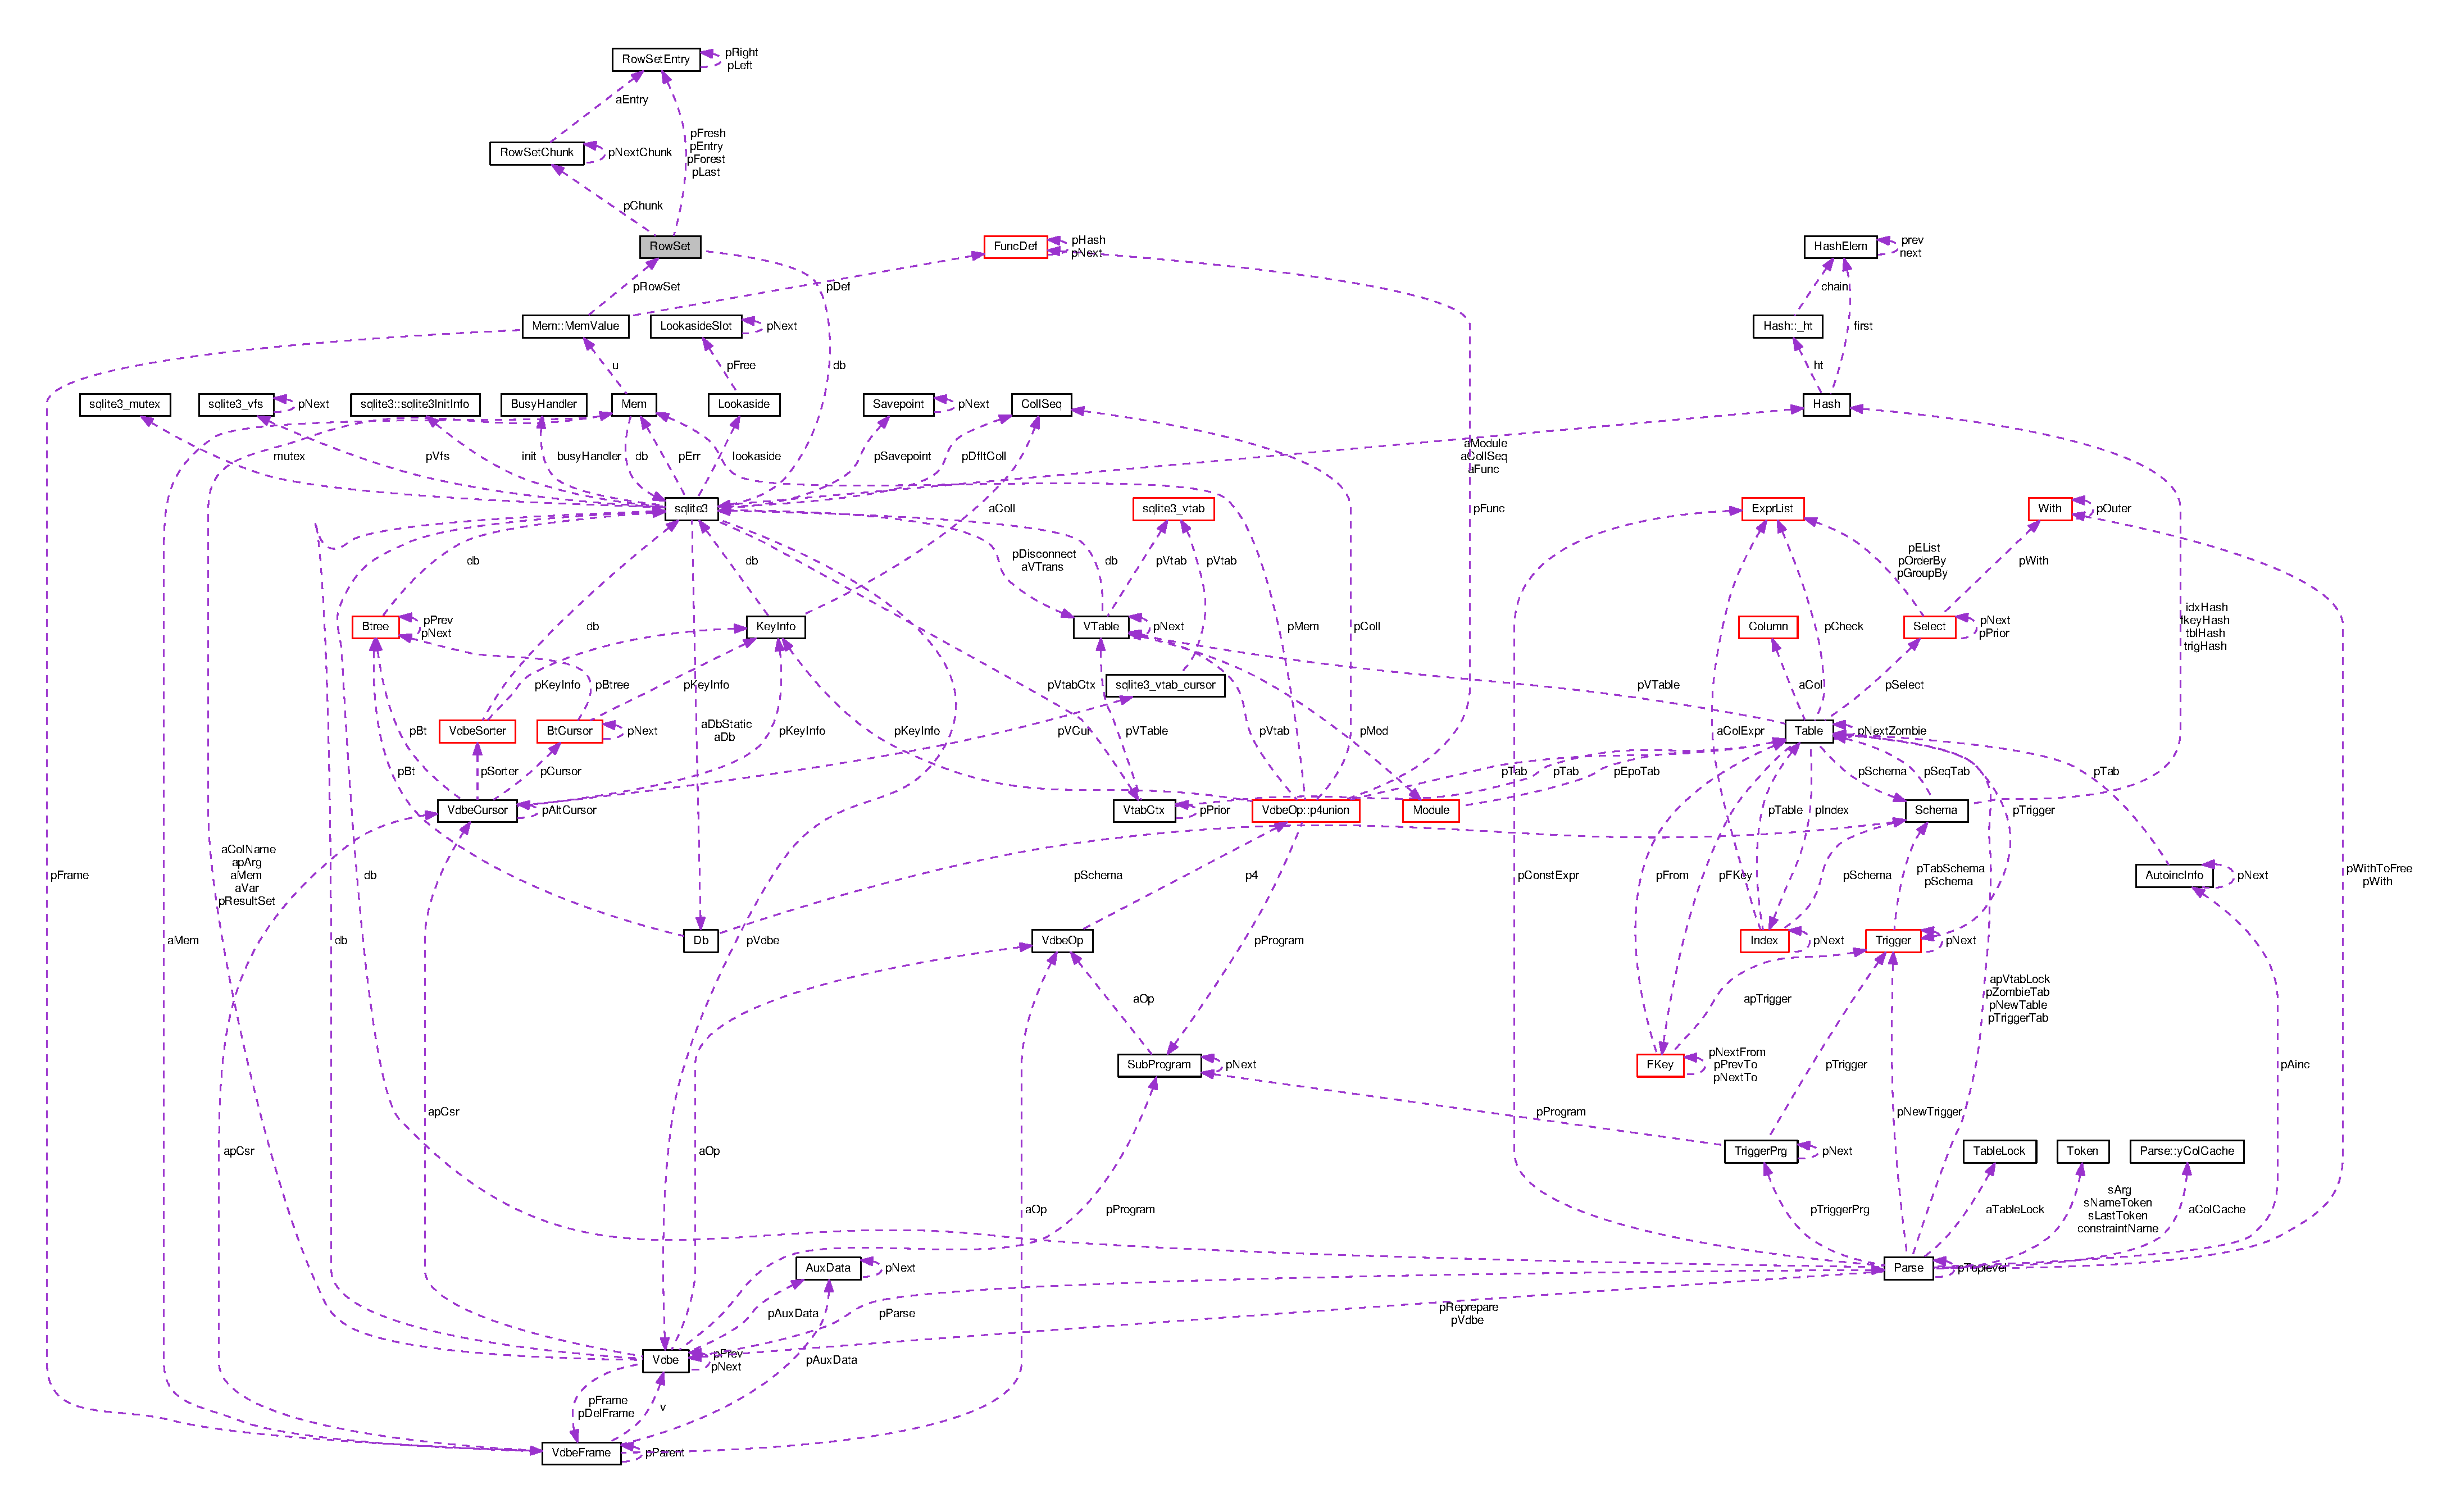
\includegraphics[width=350pt]{structRowSet__coll__graph}
\end{center}
\end{figure}
\subsection*{Public Attributes}
\begin{DoxyCompactItemize}
\item 
struct \hyperlink{structRowSetChunk}{Row\+Set\+Chunk} $\ast$ {\bfseries p\+Chunk}\hypertarget{structRowSet_af064f9ec7b1ba820a3d53622bde9d42f}{}\label{structRowSet_af064f9ec7b1ba820a3d53622bde9d42f}

\item 
\hyperlink{structsqlite3}{sqlite3} $\ast$ {\bfseries db}\hypertarget{structRowSet_a7da847a06c2f90025fbd89c57516c6f6}{}\label{structRowSet_a7da847a06c2f90025fbd89c57516c6f6}

\item 
struct \hyperlink{structRowSetEntry}{Row\+Set\+Entry} $\ast$ {\bfseries p\+Entry}\hypertarget{structRowSet_a3eccaf69ad7863abae2541a7c0b94e1d}{}\label{structRowSet_a3eccaf69ad7863abae2541a7c0b94e1d}

\item 
struct \hyperlink{structRowSetEntry}{Row\+Set\+Entry} $\ast$ {\bfseries p\+Last}\hypertarget{structRowSet_a040c4b798e6f20d20aa99a45e93b2079}{}\label{structRowSet_a040c4b798e6f20d20aa99a45e93b2079}

\item 
struct \hyperlink{structRowSetEntry}{Row\+Set\+Entry} $\ast$ {\bfseries p\+Fresh}\hypertarget{structRowSet_a7c4e95bd08ff77135068bb3987be5ca1}{}\label{structRowSet_a7c4e95bd08ff77135068bb3987be5ca1}

\item 
struct \hyperlink{structRowSetEntry}{Row\+Set\+Entry} $\ast$ {\bfseries p\+Forest}\hypertarget{structRowSet_abe7ab16fffbe5992f637d6a17c6342ff}{}\label{structRowSet_abe7ab16fffbe5992f637d6a17c6342ff}

\item 
u16 {\bfseries n\+Fresh}\hypertarget{structRowSet_a0ed2a47d6789a70081f3454ef2604e7f}{}\label{structRowSet_a0ed2a47d6789a70081f3454ef2604e7f}

\item 
u16 {\bfseries rs\+Flags}\hypertarget{structRowSet_abfbd103e329e88d0a09ca5a7c9bbd225}{}\label{structRowSet_abfbd103e329e88d0a09ca5a7c9bbd225}

\item 
int {\bfseries i\+Batch}\hypertarget{structRowSet_a90ebc79619b880c1a38b96622ad0ffe0}{}\label{structRowSet_a90ebc79619b880c1a38b96622ad0ffe0}

\end{DoxyCompactItemize}


The documentation for this struct was generated from the following file\+:\begin{DoxyCompactItemize}
\item 
sqlite3.\+c\end{DoxyCompactItemize}

\hypertarget{structRowSetChunk}{}\section{Row\+Set\+Chunk Struct Reference}
\label{structRowSetChunk}\index{Row\+Set\+Chunk@{Row\+Set\+Chunk}}


Collaboration diagram for Row\+Set\+Chunk\+:
% FIG 0
\subsection*{Public Attributes}
\begin{DoxyCompactItemize}
\item 
struct \hyperlink{structRowSetChunk}{Row\+Set\+Chunk} $\ast$ {\bfseries p\+Next\+Chunk}\hypertarget{structRowSetChunk_ae8f0975c86633ae2bb8b212d3a767554}{}\label{structRowSetChunk_ae8f0975c86633ae2bb8b212d3a767554}

\item 
struct \hyperlink{structRowSetEntry}{Row\+Set\+Entry} {\bfseries a\+Entry} \mbox{[}R\+O\+W\+S\+E\+T\+\_\+\+E\+N\+T\+R\+Y\+\_\+\+P\+E\+R\+\_\+\+C\+H\+U\+NK\mbox{]}\hypertarget{structRowSetChunk_abde97bbb07c3bf9454e719ff860bdd1f}{}\label{structRowSetChunk_abde97bbb07c3bf9454e719ff860bdd1f}

\end{DoxyCompactItemize}


The documentation for this struct was generated from the following file\+:\begin{DoxyCompactItemize}
\item 
sqlite3.\+c\end{DoxyCompactItemize}

\hypertarget{structRowSetEntry}{}\section{Row\+Set\+Entry Struct Reference}
\label{structRowSetEntry}\index{Row\+Set\+Entry@{Row\+Set\+Entry}}


Collaboration diagram for Row\+Set\+Entry\+:\nopagebreak
\begin{figure}[H]
\begin{center}
\leavevmode
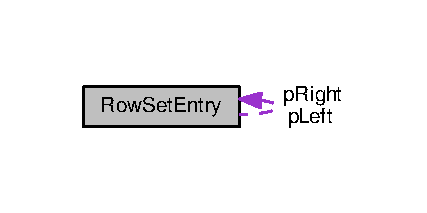
\includegraphics[width=205pt]{structRowSetEntry__coll__graph}
\end{center}
\end{figure}
\subsection*{Public Attributes}
\begin{DoxyCompactItemize}
\item 
i64 {\bfseries v}\hypertarget{structRowSetEntry_ac72670935246f1bff5e4d96703574071}{}\label{structRowSetEntry_ac72670935246f1bff5e4d96703574071}

\item 
struct \hyperlink{structRowSetEntry}{Row\+Set\+Entry} $\ast$ {\bfseries p\+Right}\hypertarget{structRowSetEntry_ac39c09525dd24f42af522587d1bc5026}{}\label{structRowSetEntry_ac39c09525dd24f42af522587d1bc5026}

\item 
struct \hyperlink{structRowSetEntry}{Row\+Set\+Entry} $\ast$ {\bfseries p\+Left}\hypertarget{structRowSetEntry_a59365203c30ce782ae38e534c90db14b}{}\label{structRowSetEntry_a59365203c30ce782ae38e534c90db14b}

\end{DoxyCompactItemize}


The documentation for this struct was generated from the following file\+:\begin{DoxyCompactItemize}
\item 
sqlite3.\+c\end{DoxyCompactItemize}

\hypertarget{structSavedModeInfo}{}\section{Saved\+Mode\+Info Struct Reference}
\label{structSavedModeInfo}\index{Saved\+Mode\+Info@{Saved\+Mode\+Info}}
\subsection*{Public Attributes}
\begin{DoxyCompactItemize}
\item 
int {\bfseries valid}\hypertarget{structSavedModeInfo_a43e863fb285c2aad913087572ebd5e27}{}\label{structSavedModeInfo_a43e863fb285c2aad913087572ebd5e27}

\item 
int {\bfseries mode}\hypertarget{structSavedModeInfo_ab6d30b28565d51ca017904f70b5edac6}{}\label{structSavedModeInfo_ab6d30b28565d51ca017904f70b5edac6}

\item 
int {\bfseries show\+Header}\hypertarget{structSavedModeInfo_a73fa5b451f94fa75fb5e27887831b8f4}{}\label{structSavedModeInfo_a73fa5b451f94fa75fb5e27887831b8f4}

\item 
int {\bfseries col\+Width} \mbox{[}100\mbox{]}\hypertarget{structSavedModeInfo_add96e86a9293b5e1bfd3ab92bf1a365f}{}\label{structSavedModeInfo_add96e86a9293b5e1bfd3ab92bf1a365f}

\end{DoxyCompactItemize}


The documentation for this struct was generated from the following file\+:\begin{DoxyCompactItemize}
\item 
shell.\+c\end{DoxyCompactItemize}

\hypertarget{structSavepoint}{}\section{Savepoint Struct Reference}
\label{structSavepoint}\index{Savepoint@{Savepoint}}


Collaboration diagram for Savepoint\+:\nopagebreak
\begin{figure}[H]
\begin{center}
\leavevmode
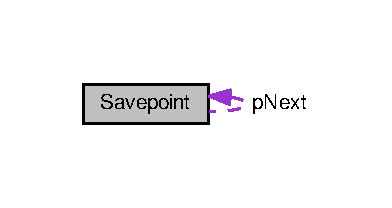
\includegraphics[width=188pt]{structSavepoint__coll__graph}
\end{center}
\end{figure}
\subsection*{Public Attributes}
\begin{DoxyCompactItemize}
\item 
char $\ast$ {\bfseries z\+Name}\hypertarget{structSavepoint_a0ba08ea77fcfd93099288375e2e9b1ec}{}\label{structSavepoint_a0ba08ea77fcfd93099288375e2e9b1ec}

\item 
i64 {\bfseries n\+Deferred\+Cons}\hypertarget{structSavepoint_ae00dd8f725701d9e31da2edbb0b27435}{}\label{structSavepoint_ae00dd8f725701d9e31da2edbb0b27435}

\item 
i64 {\bfseries n\+Deferred\+Imm\+Cons}\hypertarget{structSavepoint_a91b8cb5fac1bdf7d8f76ec30c82b862d}{}\label{structSavepoint_a91b8cb5fac1bdf7d8f76ec30c82b862d}

\item 
\hyperlink{structSavepoint}{Savepoint} $\ast$ {\bfseries p\+Next}\hypertarget{structSavepoint_a8d785c3c0eeb6f0c62ea5391892c78cb}{}\label{structSavepoint_a8d785c3c0eeb6f0c62ea5391892c78cb}

\end{DoxyCompactItemize}


The documentation for this struct was generated from the following file\+:\begin{DoxyCompactItemize}
\item 
sqlite3.\+c\end{DoxyCompactItemize}

\hypertarget{structScanStatus}{}\section{Scan\+Status Struct Reference}
\label{structScanStatus}\index{Scan\+Status@{Scan\+Status}}
\subsection*{Public Attributes}
\begin{DoxyCompactItemize}
\item 
int {\bfseries addr\+Explain}\hypertarget{structScanStatus_a621d9ae1f07b7730f1e5e2a5a0473a2e}{}\label{structScanStatus_a621d9ae1f07b7730f1e5e2a5a0473a2e}

\item 
int {\bfseries addr\+Loop}\hypertarget{structScanStatus_a9a6acff15920d8de4b97a3d3fd6781d9}{}\label{structScanStatus_a9a6acff15920d8de4b97a3d3fd6781d9}

\item 
int {\bfseries addr\+Visit}\hypertarget{structScanStatus_a31523fd6dd0dfca1233b51606140b740}{}\label{structScanStatus_a31523fd6dd0dfca1233b51606140b740}

\item 
int {\bfseries i\+Select\+ID}\hypertarget{structScanStatus_a04e5536574db523ebfcdbecdfa39568a}{}\label{structScanStatus_a04e5536574db523ebfcdbecdfa39568a}

\item 
Log\+Est {\bfseries n\+Est}\hypertarget{structScanStatus_af8666388f46040047c5e4bc9097d0336}{}\label{structScanStatus_af8666388f46040047c5e4bc9097d0336}

\item 
char $\ast$ {\bfseries z\+Name}\hypertarget{structScanStatus_ae88705a0b24b1bde60c87cdbde902c24}{}\label{structScanStatus_ae88705a0b24b1bde60c87cdbde902c24}

\end{DoxyCompactItemize}


The documentation for this struct was generated from the following file\+:\begin{DoxyCompactItemize}
\item 
sqlite3.\+c\end{DoxyCompactItemize}

\hypertarget{structSchema}{}\section{Schema Struct Reference}
\label{structSchema}\index{Schema@{Schema}}


Collaboration diagram for Schema\+:
% FIG 0
\subsection*{Public Attributes}
\begin{DoxyCompactItemize}
\item 
int {\bfseries schema\+\_\+cookie}\hypertarget{structSchema_a3eef54a64f4f962d64577646bd34a47c}{}\label{structSchema_a3eef54a64f4f962d64577646bd34a47c}

\item 
int {\bfseries i\+Generation}\hypertarget{structSchema_a879b1597656c7cbcbb98cdb88e876874}{}\label{structSchema_a879b1597656c7cbcbb98cdb88e876874}

\item 
\hyperlink{structHash}{Hash} {\bfseries tbl\+Hash}\hypertarget{structSchema_af841eadc93b289944b95f72b784bfaae}{}\label{structSchema_af841eadc93b289944b95f72b784bfaae}

\item 
\hyperlink{structHash}{Hash} {\bfseries idx\+Hash}\hypertarget{structSchema_ac0dd242f486d17ddadca1e47af76c6c5}{}\label{structSchema_ac0dd242f486d17ddadca1e47af76c6c5}

\item 
\hyperlink{structHash}{Hash} {\bfseries trig\+Hash}\hypertarget{structSchema_ab521f4545d200329d8e1a46bbb67e7c5}{}\label{structSchema_ab521f4545d200329d8e1a46bbb67e7c5}

\item 
\hyperlink{structHash}{Hash} {\bfseries fkey\+Hash}\hypertarget{structSchema_ad51ed96351701cfe8d9e871722827c11}{}\label{structSchema_ad51ed96351701cfe8d9e871722827c11}

\item 
\hyperlink{structTable}{Table} $\ast$ {\bfseries p\+Seq\+Tab}\hypertarget{structSchema_ad580e4e662724bee95571d297f94da37}{}\label{structSchema_ad580e4e662724bee95571d297f94da37}

\item 
u8 {\bfseries file\+\_\+format}\hypertarget{structSchema_ab9f0371436e41b3080772995407a4cca}{}\label{structSchema_ab9f0371436e41b3080772995407a4cca}

\item 
u8 {\bfseries enc}\hypertarget{structSchema_a1338d09fe9cbb5a8162929202cb73cae}{}\label{structSchema_a1338d09fe9cbb5a8162929202cb73cae}

\item 
u16 {\bfseries schema\+Flags}\hypertarget{structSchema_a19310cba7982138909683b1801258c18}{}\label{structSchema_a19310cba7982138909683b1801258c18}

\item 
int {\bfseries cache\+\_\+size}\hypertarget{structSchema_a0a66691be95a30c099ca4840da7110dd}{}\label{structSchema_a0a66691be95a30c099ca4840da7110dd}

\end{DoxyCompactItemize}


The documentation for this struct was generated from the following file\+:\begin{DoxyCompactItemize}
\item 
sqlite3.\+c\end{DoxyCompactItemize}

\hypertarget{structFKey_1_1sColMap}{}\section{F\+Key\+:\+:s\+Col\+Map Struct Reference}
\label{structFKey_1_1sColMap}\index{F\+Key\+::s\+Col\+Map@{F\+Key\+::s\+Col\+Map}}
\subsection*{Public Attributes}
\begin{DoxyCompactItemize}
\item 
int {\bfseries i\+From}\hypertarget{structFKey_1_1sColMap_a2b0ed19d4924a93d1f3f14f891b176ed}{}\label{structFKey_1_1sColMap_a2b0ed19d4924a93d1f3f14f891b176ed}

\item 
char $\ast$ {\bfseries z\+Col}\hypertarget{structFKey_1_1sColMap_a4cdef475be73cc460873051a2c2c2937}{}\label{structFKey_1_1sColMap_a4cdef475be73cc460873051a2c2c2937}

\end{DoxyCompactItemize}


The documentation for this struct was generated from the following file\+:\begin{DoxyCompactItemize}
\item 
sqlite3.\+c\end{DoxyCompactItemize}

\hypertarget{structScratchFreeslot}{}\section{Scratch\+Freeslot Struct Reference}
\label{structScratchFreeslot}\index{Scratch\+Freeslot@{Scratch\+Freeslot}}


Collaboration diagram for Scratch\+Freeslot\+:\nopagebreak
\begin{figure}[H]
\begin{center}
\leavevmode
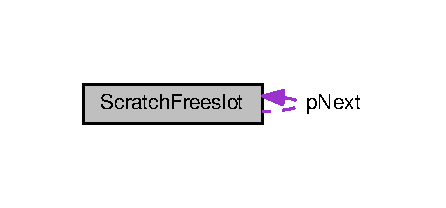
\includegraphics[width=214pt]{structScratchFreeslot__coll__graph}
\end{center}
\end{figure}
\subsection*{Public Attributes}
\begin{DoxyCompactItemize}
\item 
struct \hyperlink{structScratchFreeslot}{Scratch\+Freeslot} $\ast$ {\bfseries p\+Next}\hypertarget{structScratchFreeslot_aca5c55a56a2a63a5be0756707a04bee8}{}\label{structScratchFreeslot_aca5c55a56a2a63a5be0756707a04bee8}

\end{DoxyCompactItemize}


The documentation for this struct was generated from the following file\+:\begin{DoxyCompactItemize}
\item 
sqlite3.\+c\end{DoxyCompactItemize}

\hypertarget{structSelect}{}\section{Select Struct Reference}
\label{structSelect}\index{Select@{Select}}


Collaboration diagram for Select\+:\nopagebreak
\begin{figure}[H]
\begin{center}
\leavevmode
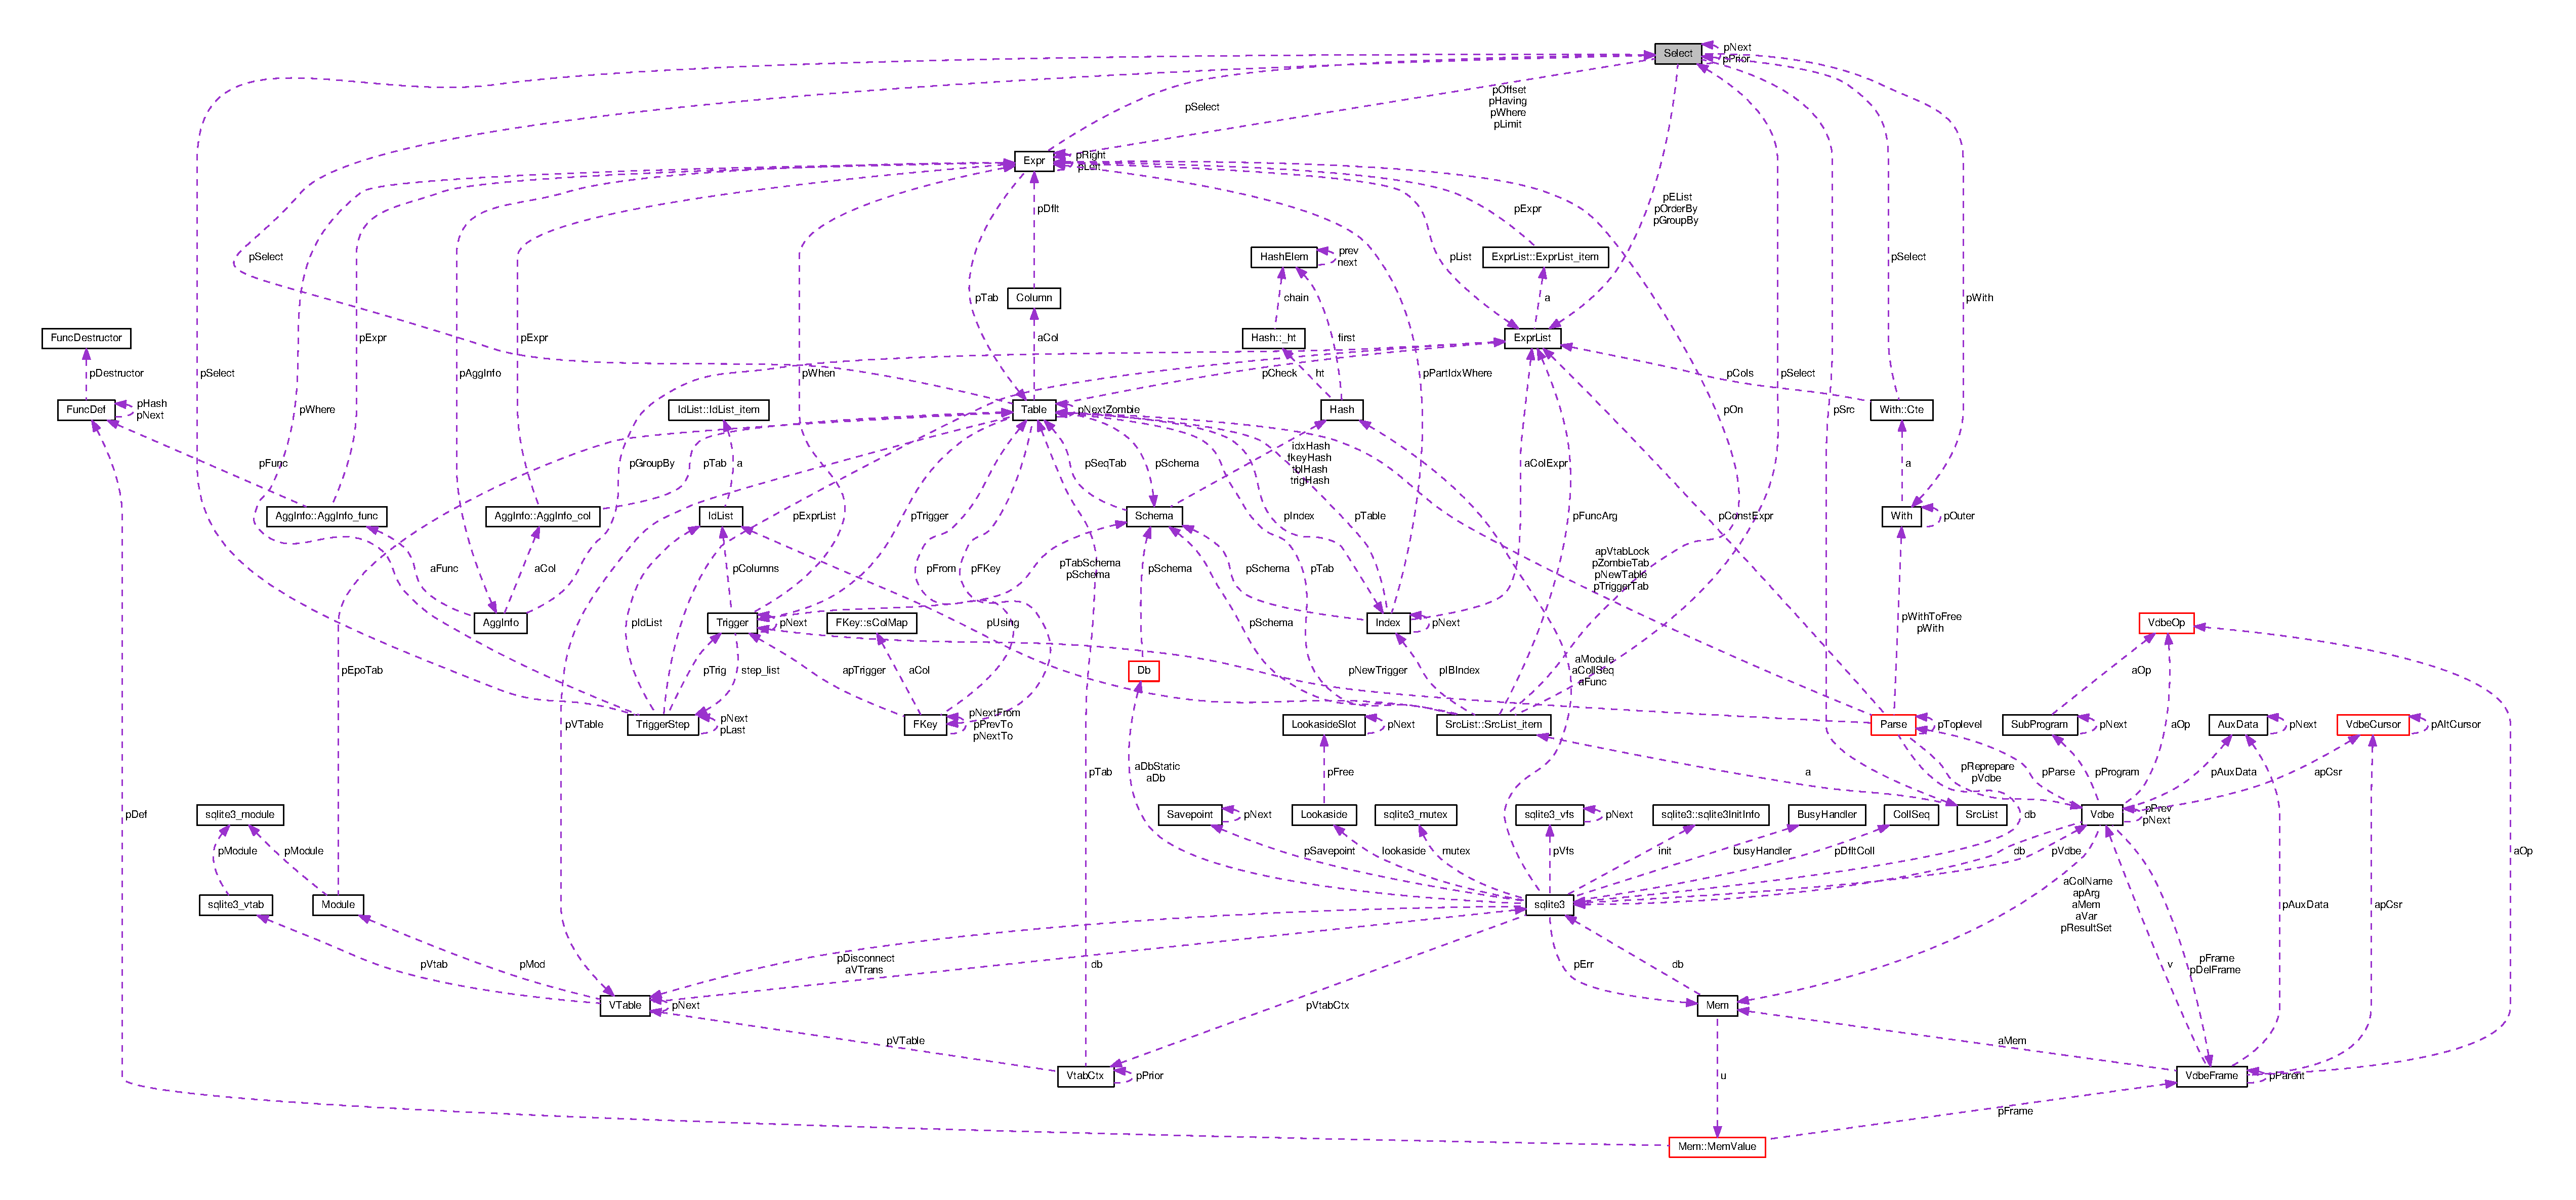
\includegraphics[width=350pt]{structSelect__coll__graph}
\end{center}
\end{figure}
\subsection*{Public Attributes}
\begin{DoxyCompactItemize}
\item 
\hyperlink{structExprList}{Expr\+List} $\ast$ {\bfseries p\+E\+List}\hypertarget{structSelect_acf92c5d6b0e0e6a3263a77696baaadc8}{}\label{structSelect_acf92c5d6b0e0e6a3263a77696baaadc8}

\item 
u8 {\bfseries op}\hypertarget{structSelect_a84506d61248313b5e10f7891cb7482be}{}\label{structSelect_a84506d61248313b5e10f7891cb7482be}

\item 
Log\+Est {\bfseries n\+Select\+Row}\hypertarget{structSelect_af9e46e47a41ceb9815690851f7e88219}{}\label{structSelect_af9e46e47a41ceb9815690851f7e88219}

\item 
u32 {\bfseries sel\+Flags}\hypertarget{structSelect_a8114a0684cb5f38d5f6ef3855114c928}{}\label{structSelect_a8114a0684cb5f38d5f6ef3855114c928}

\item 
int {\bfseries i\+Limit}\hypertarget{structSelect_abf68908bf029af42a32c60a2558a8b1e}{}\label{structSelect_abf68908bf029af42a32c60a2558a8b1e}

\item 
int {\bfseries i\+Offset}\hypertarget{structSelect_ac12bebd00ed988df3ad1efb8e6c63fe4}{}\label{structSelect_ac12bebd00ed988df3ad1efb8e6c63fe4}

\item 
int {\bfseries addr\+Open\+Ephm} \mbox{[}2\mbox{]}\hypertarget{structSelect_a7b55849c381b5452e42313aa7aa183ec}{}\label{structSelect_a7b55849c381b5452e42313aa7aa183ec}

\item 
\hyperlink{structSrcList}{Src\+List} $\ast$ {\bfseries p\+Src}\hypertarget{structSelect_a4e3b9b176a8e1b4af988405ff1f090db}{}\label{structSelect_a4e3b9b176a8e1b4af988405ff1f090db}

\item 
\hyperlink{structExpr}{Expr} $\ast$ {\bfseries p\+Where}\hypertarget{structSelect_a0562c1e19acde263a04af015611d8ce8}{}\label{structSelect_a0562c1e19acde263a04af015611d8ce8}

\item 
\hyperlink{structExprList}{Expr\+List} $\ast$ {\bfseries p\+Group\+By}\hypertarget{structSelect_a5b625c7495468ae56ca2f214a76231a0}{}\label{structSelect_a5b625c7495468ae56ca2f214a76231a0}

\item 
\hyperlink{structExpr}{Expr} $\ast$ {\bfseries p\+Having}\hypertarget{structSelect_ad09e0b115e6e1599e3075b87dfa6e66e}{}\label{structSelect_ad09e0b115e6e1599e3075b87dfa6e66e}

\item 
\hyperlink{structExprList}{Expr\+List} $\ast$ {\bfseries p\+Order\+By}\hypertarget{structSelect_a73c474cd4a9a9b9aa4e3187d8bf2d886}{}\label{structSelect_a73c474cd4a9a9b9aa4e3187d8bf2d886}

\item 
\hyperlink{structSelect}{Select} $\ast$ {\bfseries p\+Prior}\hypertarget{structSelect_a51d1a253b0aba5a54b11b3bf3896d056}{}\label{structSelect_a51d1a253b0aba5a54b11b3bf3896d056}

\item 
\hyperlink{structSelect}{Select} $\ast$ {\bfseries p\+Next}\hypertarget{structSelect_a96aa0caf60390b8f5e88589639205c40}{}\label{structSelect_a96aa0caf60390b8f5e88589639205c40}

\item 
\hyperlink{structExpr}{Expr} $\ast$ {\bfseries p\+Limit}\hypertarget{structSelect_a11d3b48d04d58be818cdefb10aa061a0}{}\label{structSelect_a11d3b48d04d58be818cdefb10aa061a0}

\item 
\hyperlink{structExpr}{Expr} $\ast$ {\bfseries p\+Offset}\hypertarget{structSelect_aeaf016a10203b911000354122562fb46}{}\label{structSelect_aeaf016a10203b911000354122562fb46}

\item 
\hyperlink{structWith}{With} $\ast$ {\bfseries p\+With}\hypertarget{structSelect_a3ab5597bdc6b219ea03a6aca93260e9f}{}\label{structSelect_a3ab5597bdc6b219ea03a6aca93260e9f}

\end{DoxyCompactItemize}


The documentation for this struct was generated from the following file\+:\begin{DoxyCompactItemize}
\item 
sqlite3.\+c\end{DoxyCompactItemize}

\hypertarget{structSelectDest}{}\section{Select\+Dest Struct Reference}
\label{structSelectDest}\index{Select\+Dest@{Select\+Dest}}


Collaboration diagram for Select\+Dest\+:\nopagebreak
\begin{figure}[H]
\begin{center}
\leavevmode
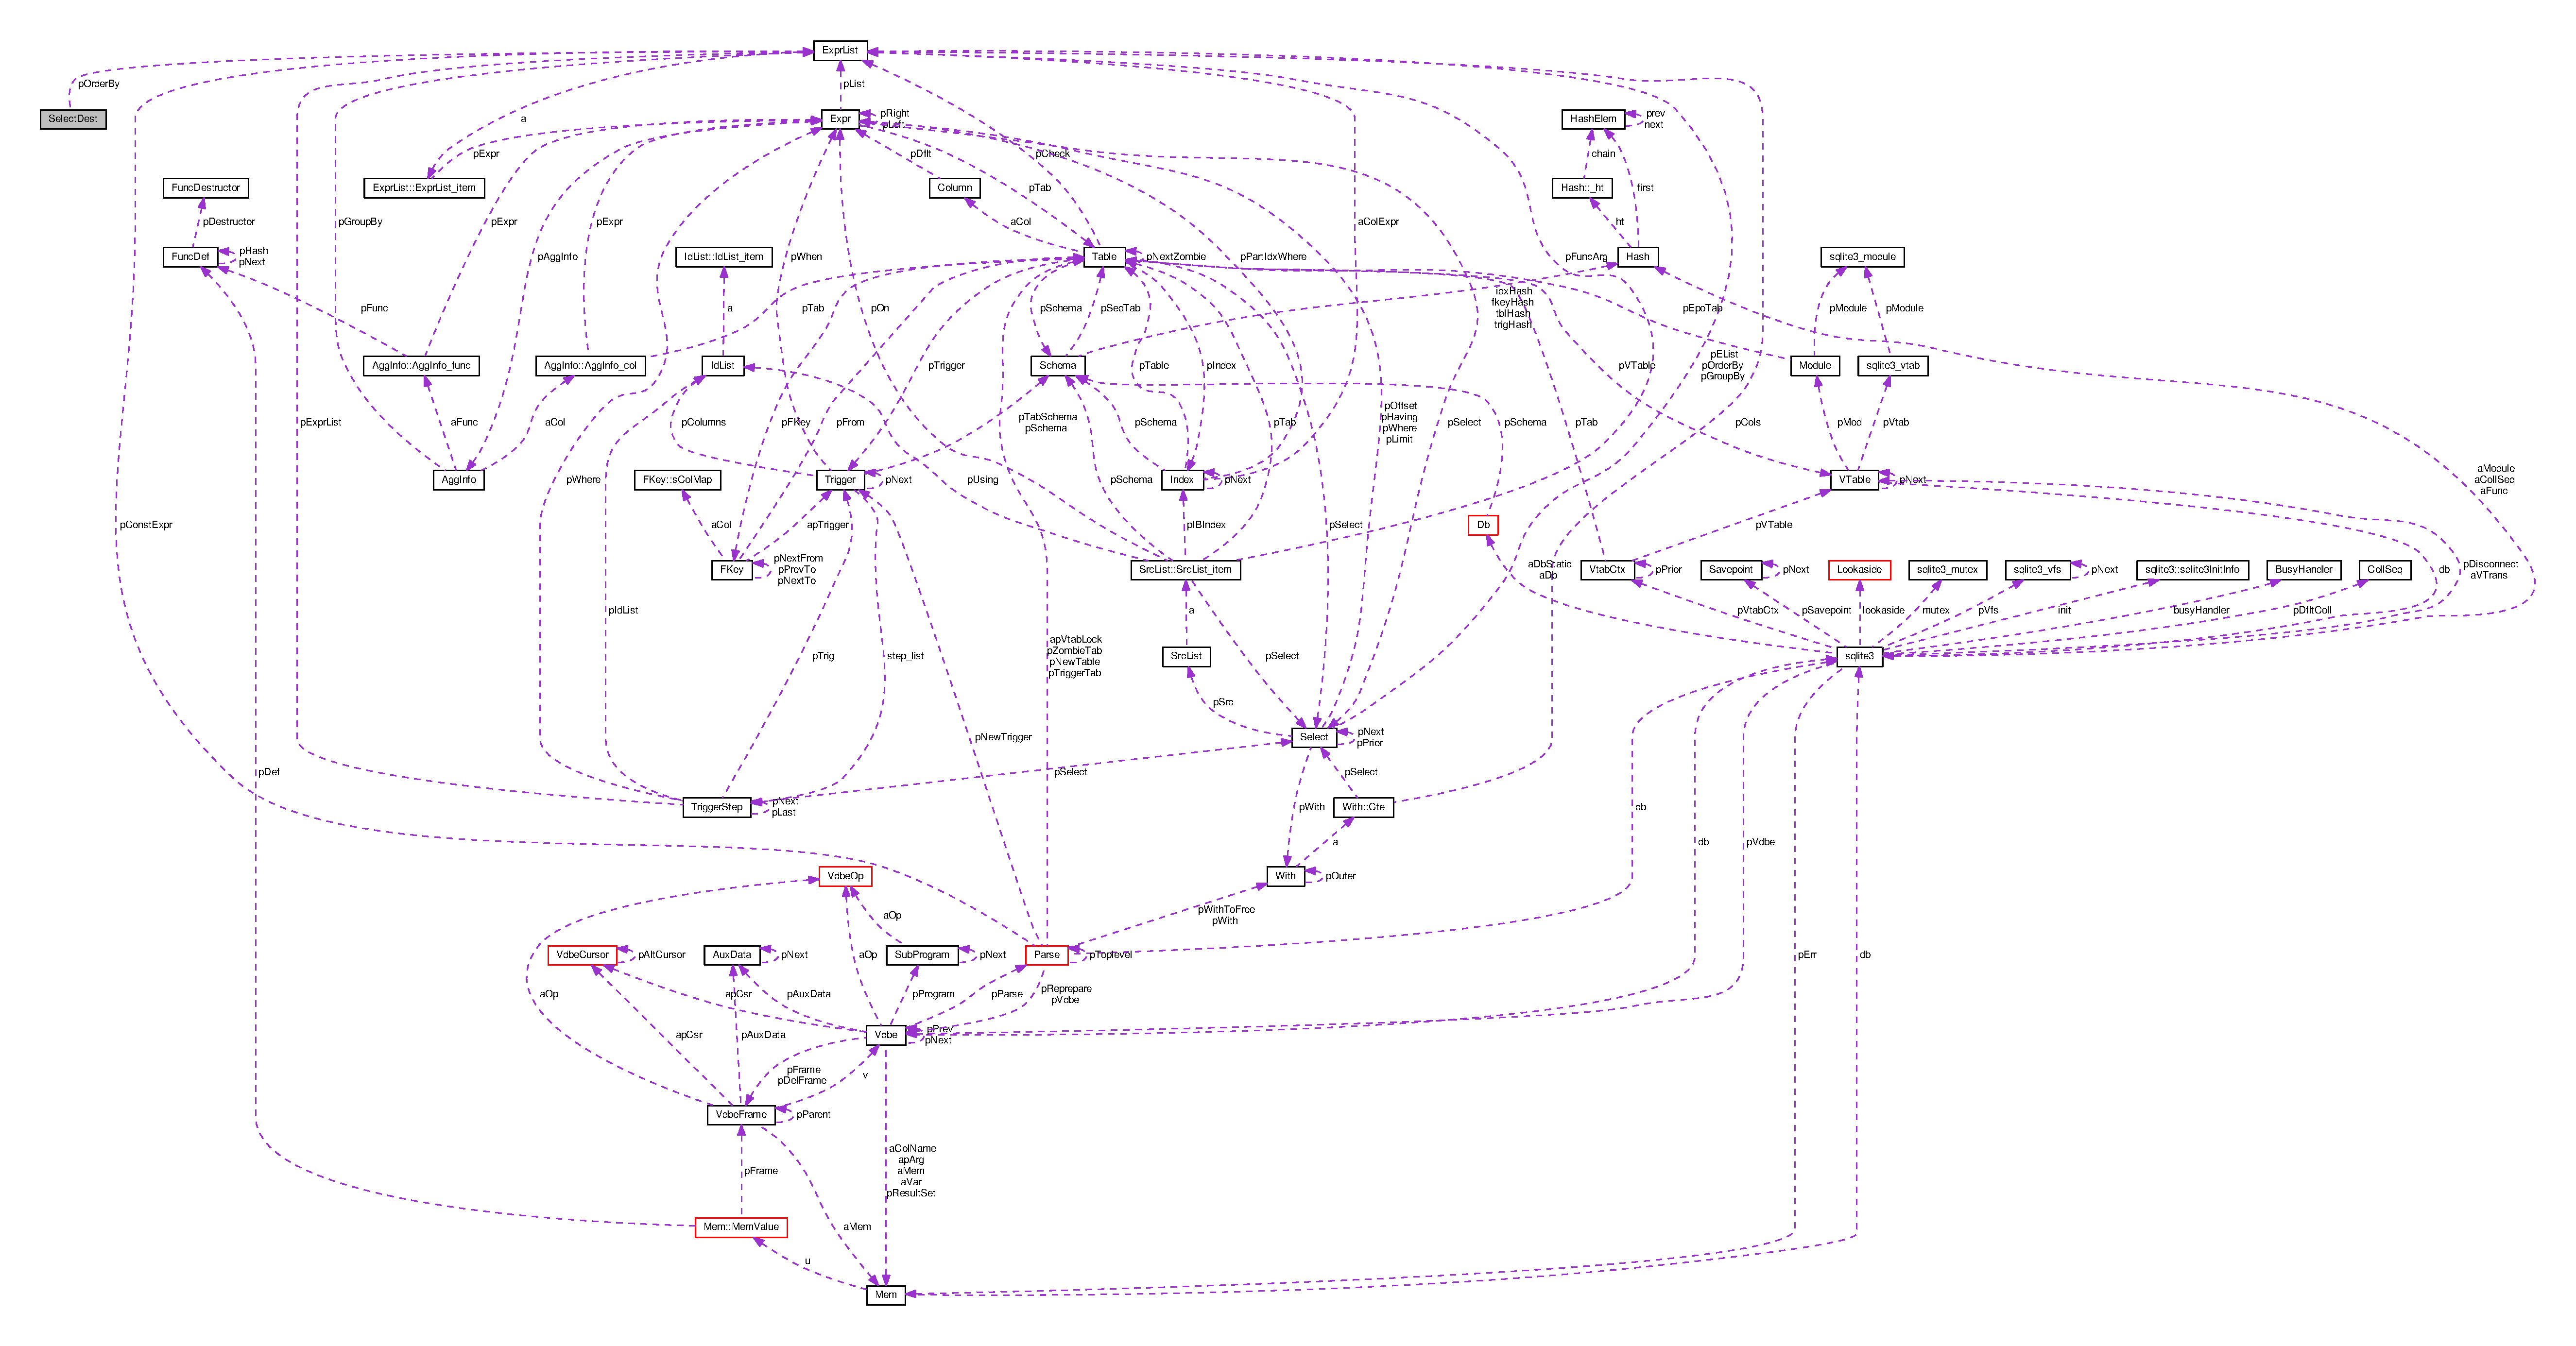
\includegraphics[width=350pt]{structSelectDest__coll__graph}
\end{center}
\end{figure}
\subsection*{Public Attributes}
\begin{DoxyCompactItemize}
\item 
u8 {\bfseries e\+Dest}\hypertarget{structSelectDest_a779c1809acadd15898db0b20e31cc23f}{}\label{structSelectDest_a779c1809acadd15898db0b20e31cc23f}

\item 
char $\ast$ {\bfseries z\+Aff\+Sdst}\hypertarget{structSelectDest_ada0376591a63aacaf9f39f9b45bb7178}{}\label{structSelectDest_ada0376591a63aacaf9f39f9b45bb7178}

\item 
int {\bfseries i\+S\+D\+Parm}\hypertarget{structSelectDest_ad30d63b2b7216a533a5ea476412664aa}{}\label{structSelectDest_ad30d63b2b7216a533a5ea476412664aa}

\item 
int {\bfseries i\+Sdst}\hypertarget{structSelectDest_adbc1c5f38b8c95da1d05e8c25dee400f}{}\label{structSelectDest_adbc1c5f38b8c95da1d05e8c25dee400f}

\item 
int {\bfseries n\+Sdst}\hypertarget{structSelectDest_aa4e7438446ef26231f7426edfda13e19}{}\label{structSelectDest_aa4e7438446ef26231f7426edfda13e19}

\item 
\hyperlink{structExprList}{Expr\+List} $\ast$ {\bfseries p\+Order\+By}\hypertarget{structSelectDest_a10881e4ffff470814a592d6d7e1541fa}{}\label{structSelectDest_a10881e4ffff470814a592d6d7e1541fa}

\end{DoxyCompactItemize}


The documentation for this struct was generated from the following file\+:\begin{DoxyCompactItemize}
\item 
sqlite3.\+c\end{DoxyCompactItemize}

\hypertarget{structShellState}{}\section{Shell\+State Struct Reference}
\label{structShellState}\index{Shell\+State@{Shell\+State}}


Collaboration diagram for Shell\+State\+:
% FIG 0
\subsection*{Public Attributes}
\begin{DoxyCompactItemize}
\item 
\hyperlink{structsqlite3}{sqlite3} $\ast$ {\bfseries db}\hypertarget{structShellState_aff5184c68cc62f6db1876cc28ffaf7e0}{}\label{structShellState_aff5184c68cc62f6db1876cc28ffaf7e0}

\item 
int {\bfseries echo\+On}\hypertarget{structShellState_a1df59448f712867b5acc5427fb929534}{}\label{structShellState_a1df59448f712867b5acc5427fb929534}

\item 
int {\bfseries auto\+Explain}\hypertarget{structShellState_a1ce80144b7c10d594fcd1cbba9b4a874}{}\label{structShellState_a1ce80144b7c10d594fcd1cbba9b4a874}

\item 
int {\bfseries auto\+E\+QP}\hypertarget{structShellState_ab3a2de04a6ec0c08da36f5b2a8870df0}{}\label{structShellState_ab3a2de04a6ec0c08da36f5b2a8870df0}

\item 
int {\bfseries stats\+On}\hypertarget{structShellState_a07631569595d0bac838efef39e6e147d}{}\label{structShellState_a07631569595d0bac838efef39e6e147d}

\item 
int {\bfseries scanstats\+On}\hypertarget{structShellState_aac5055c5404f54e65f52dfdab67cc49d}{}\label{structShellState_aac5055c5404f54e65f52dfdab67cc49d}

\item 
int {\bfseries count\+Changes}\hypertarget{structShellState_a776d2743523117e09ddbf564b3ca6731}{}\label{structShellState_a776d2743523117e09ddbf564b3ca6731}

\item 
int {\bfseries backslash\+On}\hypertarget{structShellState_afdc489576eedbfa48db76d5f3ffc9ab4}{}\label{structShellState_afdc489576eedbfa48db76d5f3ffc9ab4}

\item 
int {\bfseries out\+Count}\hypertarget{structShellState_aa3830a7924f73f6ff4eb27fd11ef4a14}{}\label{structShellState_aa3830a7924f73f6ff4eb27fd11ef4a14}

\item 
int {\bfseries cnt}\hypertarget{structShellState_a2ff4d941ad9ef12844aa5281e98ef7c1}{}\label{structShellState_a2ff4d941ad9ef12844aa5281e98ef7c1}

\item 
F\+I\+LE $\ast$ {\bfseries out}\hypertarget{structShellState_afe68611d577c5398d24a790bac1b5e56}{}\label{structShellState_afe68611d577c5398d24a790bac1b5e56}

\item 
F\+I\+LE $\ast$ {\bfseries trace\+Out}\hypertarget{structShellState_a308c221cb2f11f68231232a18466c94f}{}\label{structShellState_a308c221cb2f11f68231232a18466c94f}

\item 
int {\bfseries n\+Err}\hypertarget{structShellState_a014f654813021513e6bf6091926b3877}{}\label{structShellState_a014f654813021513e6bf6091926b3877}

\item 
int {\bfseries mode}\hypertarget{structShellState_a555e4be1ff388f8fb4e71765e4b08ab2}{}\label{structShellState_a555e4be1ff388f8fb4e71765e4b08ab2}

\item 
int {\bfseries c\+Mode}\hypertarget{structShellState_a85f31fbf107e9127829e4bbbd1a9b675}{}\label{structShellState_a85f31fbf107e9127829e4bbbd1a9b675}

\item 
int {\bfseries normal\+Mode}\hypertarget{structShellState_abf9cf08c0a0cd37b43931ed3e6b28e82}{}\label{structShellState_abf9cf08c0a0cd37b43931ed3e6b28e82}

\item 
int {\bfseries writable\+Schema}\hypertarget{structShellState_a7b6ccf04e4f4174830faf39116ed74f6}{}\label{structShellState_a7b6ccf04e4f4174830faf39116ed74f6}

\item 
int {\bfseries show\+Header}\hypertarget{structShellState_adf90aea39543d0b710b7bb6a4d0236e3}{}\label{structShellState_adf90aea39543d0b710b7bb6a4d0236e3}

\item 
int {\bfseries n\+Check}\hypertarget{structShellState_a0afb65c2cd8e373535a1323770db0040}{}\label{structShellState_a0afb65c2cd8e373535a1323770db0040}

\item 
unsigned {\bfseries shell\+Flgs}\hypertarget{structShellState_a970dc91433f4d8d1c6776d2eb9753c6f}{}\label{structShellState_a970dc91433f4d8d1c6776d2eb9753c6f}

\item 
char $\ast$ {\bfseries z\+Dest\+Table}\hypertarget{structShellState_a1019f63cae8d412dc13a06bb80562247}{}\label{structShellState_a1019f63cae8d412dc13a06bb80562247}

\item 
char {\bfseries z\+Testcase} \mbox{[}30\mbox{]}\hypertarget{structShellState_a8c9b32aa186f1b581fc57f324cad108e}{}\label{structShellState_a8c9b32aa186f1b581fc57f324cad108e}

\item 
char {\bfseries col\+Separator} \mbox{[}20\mbox{]}\hypertarget{structShellState_ae9d5cc638c180de0798aeee4f17b416b}{}\label{structShellState_ae9d5cc638c180de0798aeee4f17b416b}

\item 
char {\bfseries row\+Separator} \mbox{[}20\mbox{]}\hypertarget{structShellState_a576a4b6fd62786683bafb6c7631eae6f}{}\label{structShellState_a576a4b6fd62786683bafb6c7631eae6f}

\item 
int {\bfseries col\+Width} \mbox{[}100\mbox{]}\hypertarget{structShellState_adf07d77efc02d83f1c42500ef6a4c433}{}\label{structShellState_adf07d77efc02d83f1c42500ef6a4c433}

\item 
int {\bfseries actual\+Width} \mbox{[}100\mbox{]}\hypertarget{structShellState_ae5e87296fedf861b6013c48f20888c2b}{}\label{structShellState_ae5e87296fedf861b6013c48f20888c2b}

\item 
char {\bfseries null\+Value} \mbox{[}20\mbox{]}\hypertarget{structShellState_a6ae47309eca991773424ffd6b6dd3170}{}\label{structShellState_a6ae47309eca991773424ffd6b6dd3170}

\item 
char {\bfseries outfile} \mbox{[}F\+I\+L\+E\+N\+A\+M\+E\+\_\+\+M\+AX\mbox{]}\hypertarget{structShellState_ab1901d796d12c9fe4859f954fba74235}{}\label{structShellState_ab1901d796d12c9fe4859f954fba74235}

\item 
const char $\ast$ {\bfseries z\+Db\+Filename}\hypertarget{structShellState_a8b887b0d2047997012969639cec7aec1}{}\label{structShellState_a8b887b0d2047997012969639cec7aec1}

\item 
char $\ast$ {\bfseries z\+Free\+On\+Close}\hypertarget{structShellState_acd5673a65d8d4aa5a5a674e4ad8a374b}{}\label{structShellState_acd5673a65d8d4aa5a5a674e4ad8a374b}

\item 
const char $\ast$ {\bfseries z\+Vfs}\hypertarget{structShellState_a7a17ec105e801f6d466f3dd8e29521e6}{}\label{structShellState_a7a17ec105e801f6d466f3dd8e29521e6}

\item 
sqlite3\+\_\+stmt $\ast$ {\bfseries p\+Stmt}\hypertarget{structShellState_a443b930c7001c9b669728b917c2f5587}{}\label{structShellState_a443b930c7001c9b669728b917c2f5587}

\item 
F\+I\+LE $\ast$ {\bfseries p\+Log}\hypertarget{structShellState_a9ca42a0d7bf19e576de8ea13ba40b61c}{}\label{structShellState_a9ca42a0d7bf19e576de8ea13ba40b61c}

\item 
int $\ast$ {\bfseries ai\+Indent}\hypertarget{structShellState_a0481fdd4a0c88fb17f1a66ba87939ce9}{}\label{structShellState_a0481fdd4a0c88fb17f1a66ba87939ce9}

\item 
int {\bfseries n\+Indent}\hypertarget{structShellState_a73e3fe627474f4de6c0e04837ee0b0bd}{}\label{structShellState_a73e3fe627474f4de6c0e04837ee0b0bd}

\item 
int {\bfseries i\+Indent}\hypertarget{structShellState_a08d5d59ae0d44497aca79e89a5b8f0fe}{}\label{structShellState_a08d5d59ae0d44497aca79e89a5b8f0fe}

\end{DoxyCompactItemize}


The documentation for this struct was generated from the following file\+:\begin{DoxyCompactItemize}
\item 
shell.\+c\end{DoxyCompactItemize}

\hypertarget{structSortCtx}{}\section{Sort\+Ctx Struct Reference}
\label{structSortCtx}\index{Sort\+Ctx@{Sort\+Ctx}}


Collaboration diagram for Sort\+Ctx\+:
% FIG 0
\subsection*{Public Attributes}
\begin{DoxyCompactItemize}
\item 
\hyperlink{structExprList}{Expr\+List} $\ast$ {\bfseries p\+Order\+By}\hypertarget{structSortCtx_a4c1f59510d6e08b38c958c358d31ba07}{}\label{structSortCtx_a4c1f59510d6e08b38c958c358d31ba07}

\item 
int {\bfseries n\+O\+B\+Sat}\hypertarget{structSortCtx_a32e424bbae6b3e56a0959738eaaaf1d2}{}\label{structSortCtx_a32e424bbae6b3e56a0959738eaaaf1d2}

\item 
int {\bfseries i\+E\+Cursor}\hypertarget{structSortCtx_acaf1633a51ccc836edd0594f90ed501b}{}\label{structSortCtx_acaf1633a51ccc836edd0594f90ed501b}

\item 
int {\bfseries reg\+Return}\hypertarget{structSortCtx_a78017ace0acd29ba15652e389d9f90f6}{}\label{structSortCtx_a78017ace0acd29ba15652e389d9f90f6}

\item 
int {\bfseries label\+Bk\+Out}\hypertarget{structSortCtx_abc19dcb503656023d5596aa31378e973}{}\label{structSortCtx_abc19dcb503656023d5596aa31378e973}

\item 
int {\bfseries addr\+Sort\+Index}\hypertarget{structSortCtx_ad4c264de37b3f3b9bbff55e34659ef11}{}\label{structSortCtx_ad4c264de37b3f3b9bbff55e34659ef11}

\item 
int {\bfseries label\+Done}\hypertarget{structSortCtx_a0f08fc3dd9df4320b3bb74461ca46759}{}\label{structSortCtx_a0f08fc3dd9df4320b3bb74461ca46759}

\item 
u8 {\bfseries sort\+Flags}\hypertarget{structSortCtx_aca4654bd8cf3789c3a1b05d144e3ce2c}{}\label{structSortCtx_aca4654bd8cf3789c3a1b05d144e3ce2c}

\item 
u8 {\bfseries b\+Ordered\+Inner\+Loop}\hypertarget{structSortCtx_a193c1104dbc3f5bfef3bd1f5ae1ada03}{}\label{structSortCtx_a193c1104dbc3f5bfef3bd1f5ae1ada03}

\end{DoxyCompactItemize}


The documentation for this struct was generated from the following file\+:\begin{DoxyCompactItemize}
\item 
sqlite3.\+c\end{DoxyCompactItemize}

\hypertarget{structSorterFile}{}\section{Sorter\+File Struct Reference}
\label{structSorterFile}\index{Sorter\+File@{Sorter\+File}}


Collaboration diagram for Sorter\+File\+:\nopagebreak
\begin{figure}[H]
\begin{center}
\leavevmode
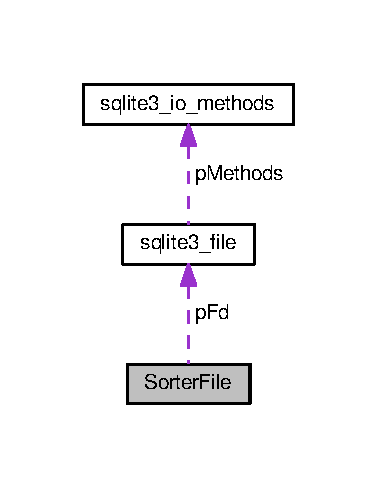
\includegraphics[width=181pt]{structSorterFile__coll__graph}
\end{center}
\end{figure}
\subsection*{Public Attributes}
\begin{DoxyCompactItemize}
\item 
\hyperlink{structsqlite3__file}{sqlite3\+\_\+file} $\ast$ {\bfseries p\+Fd}\hypertarget{structSorterFile_afa23123282380b8d04b943479cabadef}{}\label{structSorterFile_afa23123282380b8d04b943479cabadef}

\item 
i64 {\bfseries i\+Eof}\hypertarget{structSorterFile_a5c5f37fc8b5c432d8bf30eb6e40f7823}{}\label{structSorterFile_a5c5f37fc8b5c432d8bf30eb6e40f7823}

\end{DoxyCompactItemize}


The documentation for this struct was generated from the following file\+:\begin{DoxyCompactItemize}
\item 
sqlite3.\+c\end{DoxyCompactItemize}

\hypertarget{structSorterList}{}\section{Sorter\+List Struct Reference}
\label{structSorterList}\index{Sorter\+List@{Sorter\+List}}


Collaboration diagram for Sorter\+List\+:\nopagebreak
\begin{figure}[H]
\begin{center}
\leavevmode
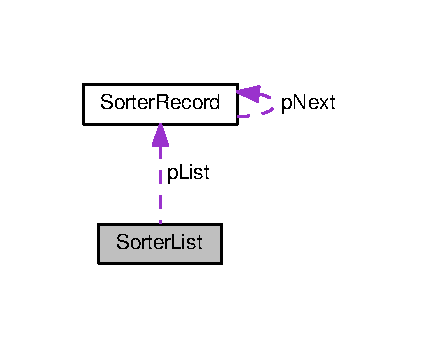
\includegraphics[width=202pt]{structSorterList__coll__graph}
\end{center}
\end{figure}
\subsection*{Public Attributes}
\begin{DoxyCompactItemize}
\item 
\hyperlink{structSorterRecord}{Sorter\+Record} $\ast$ {\bfseries p\+List}\hypertarget{structSorterList_a913640b1b917acccd7a851483f9d4e2b}{}\label{structSorterList_a913640b1b917acccd7a851483f9d4e2b}

\item 
u8 $\ast$ {\bfseries a\+Memory}\hypertarget{structSorterList_ae0c7c3714fd8c61b806a5767ce686344}{}\label{structSorterList_ae0c7c3714fd8c61b806a5767ce686344}

\item 
int {\bfseries sz\+P\+MA}\hypertarget{structSorterList_a4d14b7e48b155f6b79dd6fd37645b73c}{}\label{structSorterList_a4d14b7e48b155f6b79dd6fd37645b73c}

\end{DoxyCompactItemize}


The documentation for this struct was generated from the following file\+:\begin{DoxyCompactItemize}
\item 
sqlite3.\+c\end{DoxyCompactItemize}

\hypertarget{structSorterRecord}{}\section{Sorter\+Record Struct Reference}
\label{structSorterRecord}\index{Sorter\+Record@{Sorter\+Record}}


Collaboration diagram for Sorter\+Record\+:\nopagebreak
\begin{figure}[H]
\begin{center}
\leavevmode
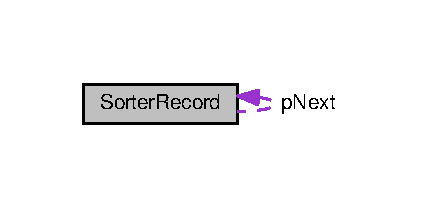
\includegraphics[width=202pt]{structSorterRecord__coll__graph}
\end{center}
\end{figure}
\subsection*{Public Attributes}
\begin{DoxyCompactItemize}
\item 
int {\bfseries n\+Val}\hypertarget{structSorterRecord_a2b8ffc0f8410826de8b41425759bf462}{}\label{structSorterRecord_a2b8ffc0f8410826de8b41425759bf462}

\item 
\begin{tabbing}
xx\=xx\=xx\=xx\=xx\=xx\=xx\=xx\=xx\=\kill
union \{\\
\>\hyperlink{structSorterRecord}{SorterRecord} $\ast$ {\bfseries pNext}\\
\>int {\bfseries iNext}\\
\} {\bfseries u}\hypertarget{structSorterRecord_a95d438d535a97eb4ed5f57d2677aaa6b}{}\label{structSorterRecord_a95d438d535a97eb4ed5f57d2677aaa6b}
\\

\end{tabbing}\end{DoxyCompactItemize}


The documentation for this struct was generated from the following file\+:\begin{DoxyCompactItemize}
\item 
sqlite3.\+c\end{DoxyCompactItemize}

\hypertarget{structSortSubtask}{}\section{Sort\+Subtask Struct Reference}
\label{structSortSubtask}\index{Sort\+Subtask@{Sort\+Subtask}}


Collaboration diagram for Sort\+Subtask\+:\nopagebreak
\begin{figure}[H]
\begin{center}
\leavevmode
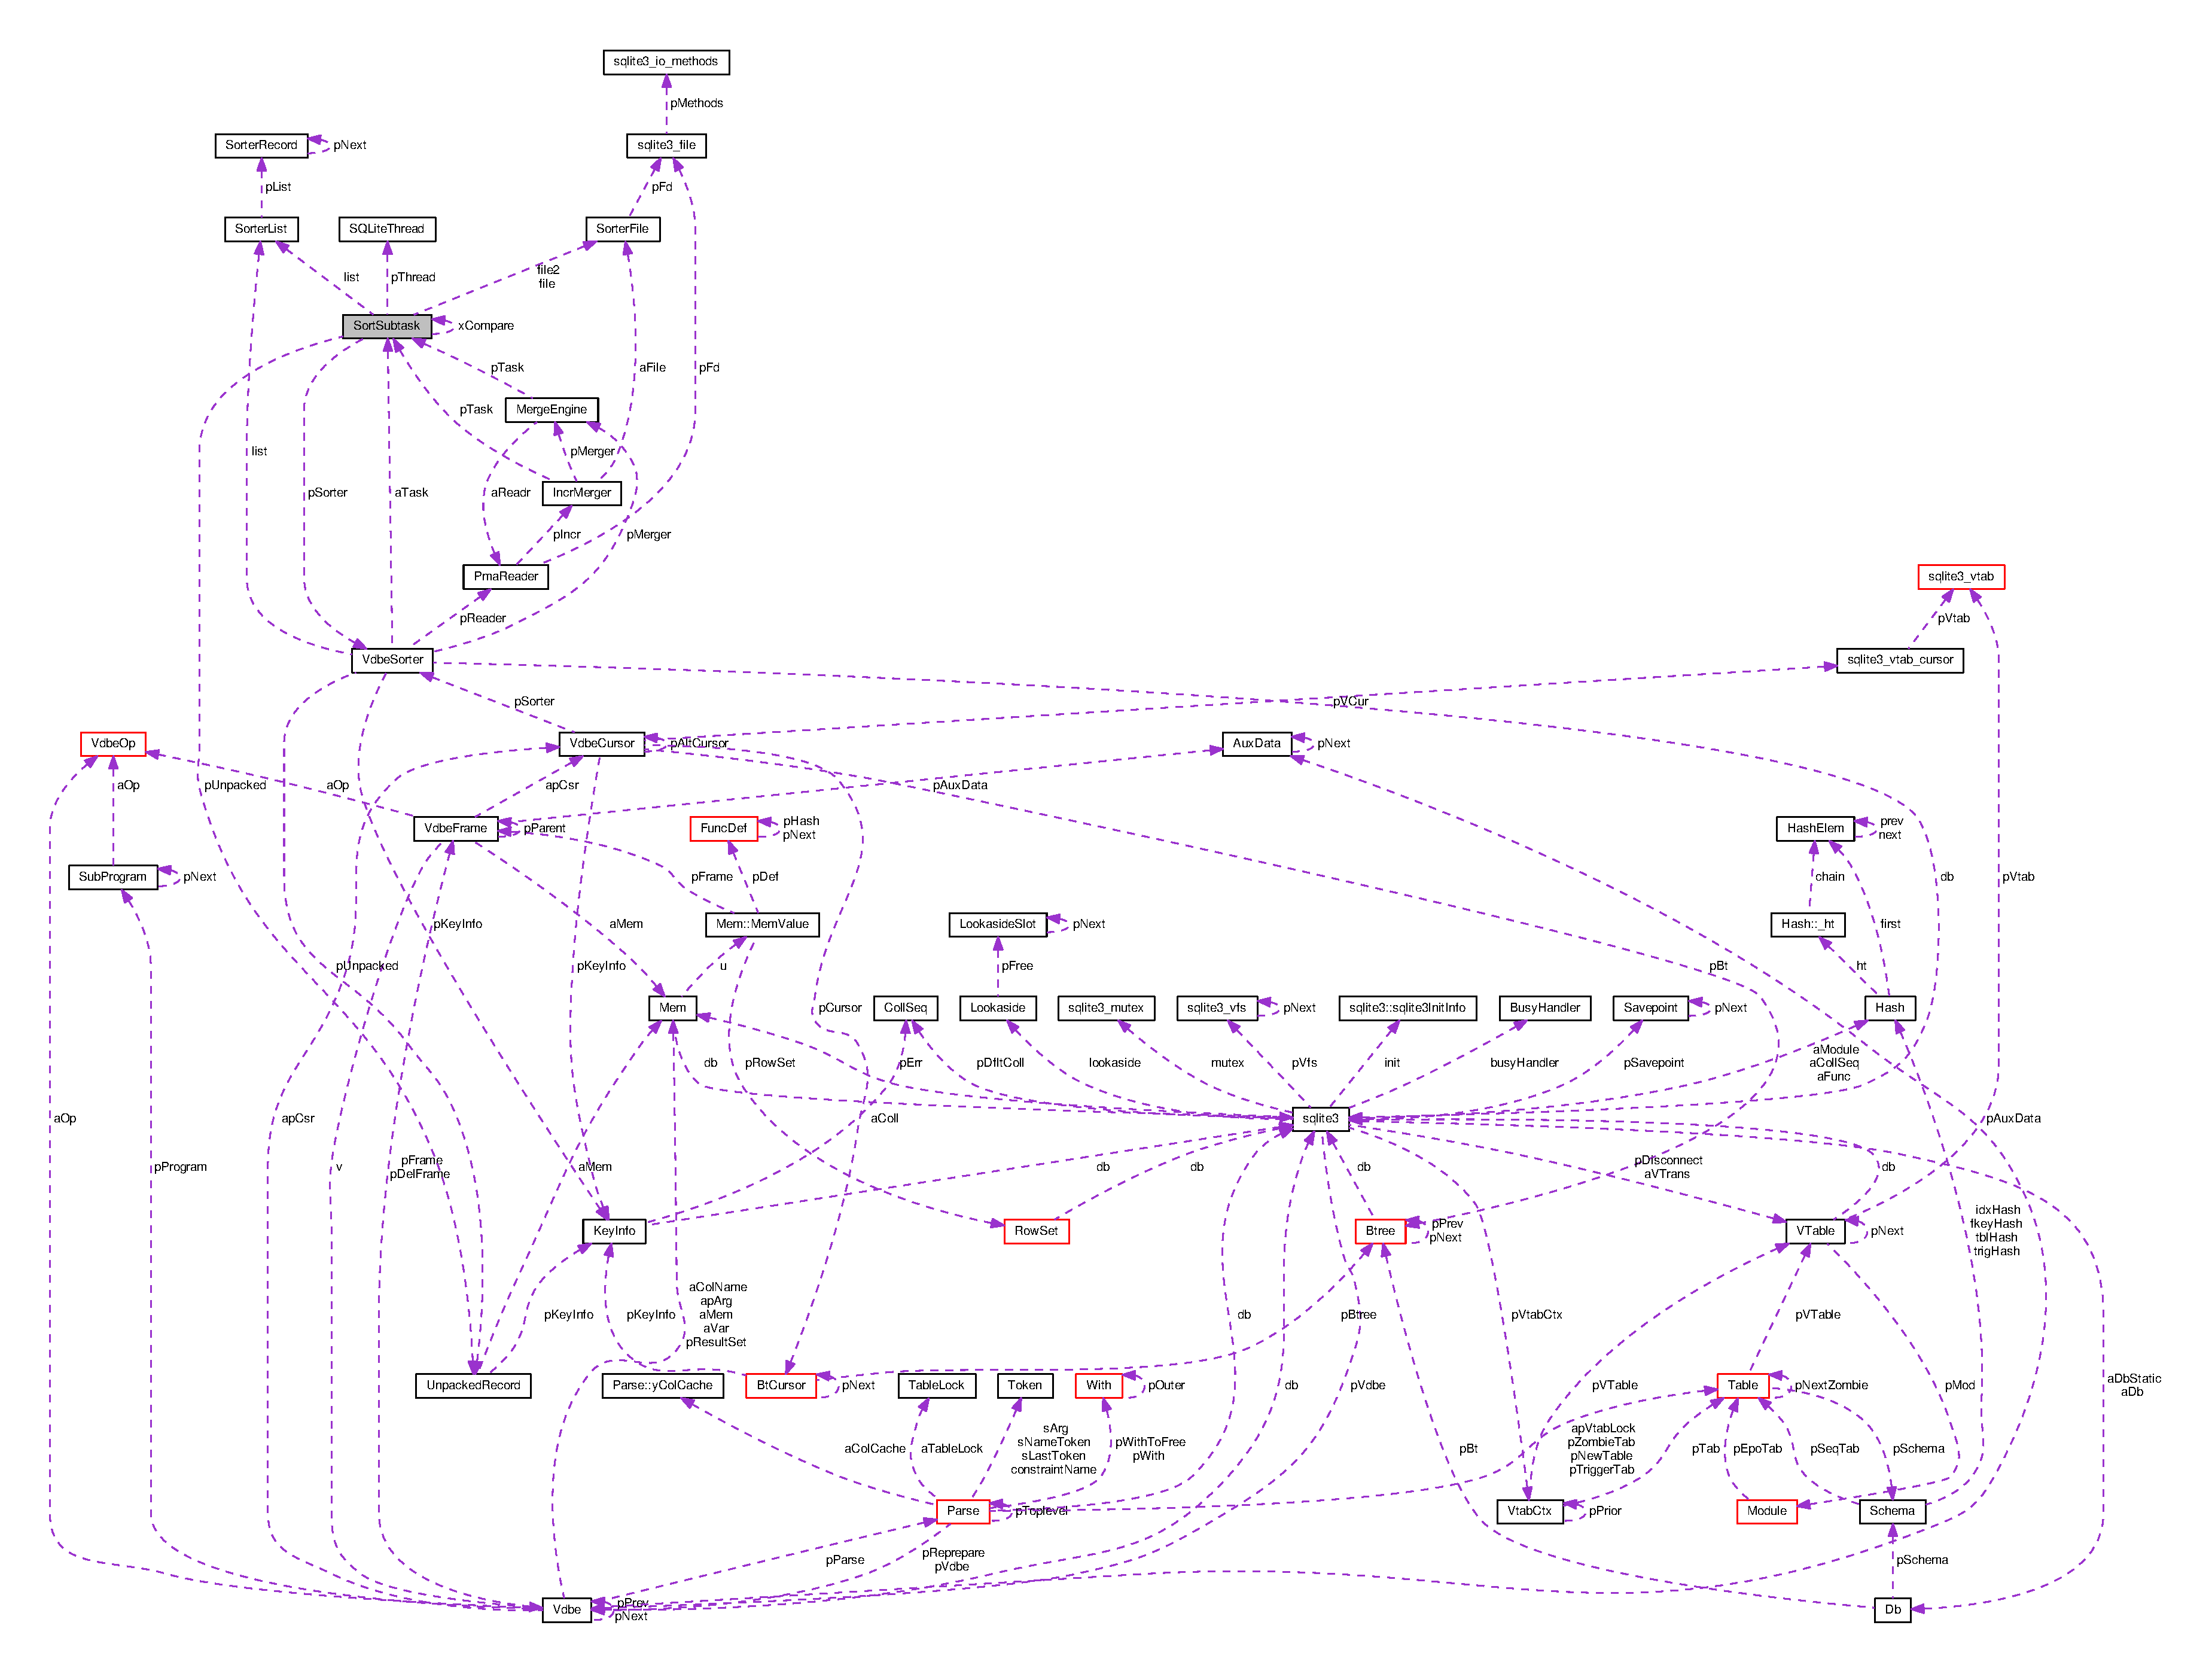
\includegraphics[width=350pt]{structSortSubtask__coll__graph}
\end{center}
\end{figure}
\subsection*{Public Attributes}
\begin{DoxyCompactItemize}
\item 
\hyperlink{structSQLiteThread}{S\+Q\+Lite\+Thread} $\ast$ {\bfseries p\+Thread}\hypertarget{structSortSubtask_abb534010ac35e0c37e41c26712e7b58c}{}\label{structSortSubtask_abb534010ac35e0c37e41c26712e7b58c}

\item 
int {\bfseries b\+Done}\hypertarget{structSortSubtask_a156fc75053f13e877c36d80885338060}{}\label{structSortSubtask_a156fc75053f13e877c36d80885338060}

\item 
\hyperlink{structVdbeSorter}{Vdbe\+Sorter} $\ast$ {\bfseries p\+Sorter}\hypertarget{structSortSubtask_a2a8ec6b4b0d29090e3b33b1a6647655a}{}\label{structSortSubtask_a2a8ec6b4b0d29090e3b33b1a6647655a}

\item 
\hyperlink{structUnpackedRecord}{Unpacked\+Record} $\ast$ {\bfseries p\+Unpacked}\hypertarget{structSortSubtask_af2312bacbb7e4cbe905eae20a60a3f39}{}\label{structSortSubtask_af2312bacbb7e4cbe905eae20a60a3f39}

\item 
\hyperlink{structSorterList}{Sorter\+List} {\bfseries list}\hypertarget{structSortSubtask_a0a79fd21798a08ceede3febbd08c88a2}{}\label{structSortSubtask_a0a79fd21798a08ceede3febbd08c88a2}

\item 
int {\bfseries n\+P\+MA}\hypertarget{structSortSubtask_a6ecceaeda562346b298aa9fb95355071}{}\label{structSortSubtask_a6ecceaeda562346b298aa9fb95355071}

\item 
Sorter\+Compare {\bfseries x\+Compare}\hypertarget{structSortSubtask_a42bfd224f9e8125c22c2cc66f865d9af}{}\label{structSortSubtask_a42bfd224f9e8125c22c2cc66f865d9af}

\item 
\hyperlink{structSorterFile}{Sorter\+File} {\bfseries file}\hypertarget{structSortSubtask_a077f999ff1e4148e48bd8df25092fd85}{}\label{structSortSubtask_a077f999ff1e4148e48bd8df25092fd85}

\item 
\hyperlink{structSorterFile}{Sorter\+File} {\bfseries file2}\hypertarget{structSortSubtask_a23b46687f7a96ef1052a062f8097234e}{}\label{structSortSubtask_a23b46687f7a96ef1052a062f8097234e}

\end{DoxyCompactItemize}


The documentation for this struct was generated from the following file\+:\begin{DoxyCompactItemize}
\item 
sqlite3.\+c\end{DoxyCompactItemize}

\hypertarget{structsqlite3}{}\section{sqlite3 Struct Reference}
\label{structsqlite3}\index{sqlite3@{sqlite3}}


Collaboration diagram for sqlite3\+:
% FIG 0
\subsection*{Classes}
\begin{DoxyCompactItemize}
\item 
struct \hyperlink{structsqlite3_1_1sqlite3InitInfo}{sqlite3\+Init\+Info}
\end{DoxyCompactItemize}
\subsection*{Public Attributes}
\begin{DoxyCompactItemize}
\item 
\hyperlink{structsqlite3__vfs}{sqlite3\+\_\+vfs} $\ast$ {\bfseries p\+Vfs}\hypertarget{structsqlite3_a8ad0bcb473e4cb492165739acff918cd}{}\label{structsqlite3_a8ad0bcb473e4cb492165739acff918cd}

\item 
struct \hyperlink{structVdbe}{Vdbe} $\ast$ {\bfseries p\+Vdbe}\hypertarget{structsqlite3_a596f0301f43c5e25575c2a1403f8b571}{}\label{structsqlite3_a596f0301f43c5e25575c2a1403f8b571}

\item 
\hyperlink{structCollSeq}{Coll\+Seq} $\ast$ {\bfseries p\+Dflt\+Coll}\hypertarget{structsqlite3_a2e5d7e7ac07c33b11c936b181d07789a}{}\label{structsqlite3_a2e5d7e7ac07c33b11c936b181d07789a}

\item 
\hyperlink{structsqlite3__mutex}{sqlite3\+\_\+mutex} $\ast$ {\bfseries mutex}\hypertarget{structsqlite3_a6328497ac0393204ab5f5083f05731c9}{}\label{structsqlite3_a6328497ac0393204ab5f5083f05731c9}

\item 
\hyperlink{structDb}{Db} $\ast$ {\bfseries a\+Db}\hypertarget{structsqlite3_a0abe1dccdea5f43e6c49360b42749697}{}\label{structsqlite3_a0abe1dccdea5f43e6c49360b42749697}

\item 
int {\bfseries n\+Db}\hypertarget{structsqlite3_a03d047bc289999b0e39d8637f0762489}{}\label{structsqlite3_a03d047bc289999b0e39d8637f0762489}

\item 
int {\bfseries flags}\hypertarget{structsqlite3_a8dac784e669d6b8a9f936d3193c1aaec}{}\label{structsqlite3_a8dac784e669d6b8a9f936d3193c1aaec}

\item 
i64 {\bfseries last\+Rowid}\hypertarget{structsqlite3_a9fff52fc4eb087fbb3e3271994fa5198}{}\label{structsqlite3_a9fff52fc4eb087fbb3e3271994fa5198}

\item 
i64 {\bfseries sz\+Mmap}\hypertarget{structsqlite3_a417e58ace305325f40894c14fbd8af0d}{}\label{structsqlite3_a417e58ace305325f40894c14fbd8af0d}

\item 
unsigned int {\bfseries open\+Flags}\hypertarget{structsqlite3_acfe8618d03dcd195a992886079c3b014}{}\label{structsqlite3_acfe8618d03dcd195a992886079c3b014}

\item 
int {\bfseries err\+Code}\hypertarget{structsqlite3_a73adbb5395118bcbd9e4d705712966a2}{}\label{structsqlite3_a73adbb5395118bcbd9e4d705712966a2}

\item 
int {\bfseries err\+Mask}\hypertarget{structsqlite3_a12541dafcf60cfce52fb60f84e42f152}{}\label{structsqlite3_a12541dafcf60cfce52fb60f84e42f152}

\item 
int {\bfseries i\+Sys\+Errno}\hypertarget{structsqlite3_ace6e1a4f7d28246883bde14b3b12c26b}{}\label{structsqlite3_ace6e1a4f7d28246883bde14b3b12c26b}

\item 
u16 {\bfseries db\+Opt\+Flags}\hypertarget{structsqlite3_ad4f903754af81d1e646bf966312f9c37}{}\label{structsqlite3_ad4f903754af81d1e646bf966312f9c37}

\item 
u8 {\bfseries enc}\hypertarget{structsqlite3_abad75b8b6663c237060656d1ae715e45}{}\label{structsqlite3_abad75b8b6663c237060656d1ae715e45}

\item 
u8 {\bfseries auto\+Commit}\hypertarget{structsqlite3_a11baf5e051b2e4ea03c5d03c09bb624e}{}\label{structsqlite3_a11baf5e051b2e4ea03c5d03c09bb624e}

\item 
u8 {\bfseries temp\+\_\+store}\hypertarget{structsqlite3_acc46921b20f505ddce64526cac717af3}{}\label{structsqlite3_acc46921b20f505ddce64526cac717af3}

\item 
u8 {\bfseries malloc\+Failed}\hypertarget{structsqlite3_a79beb0036337ba7fc2de5ccbb9225935}{}\label{structsqlite3_a79beb0036337ba7fc2de5ccbb9225935}

\item 
u8 {\bfseries b\+Benign\+Malloc}\hypertarget{structsqlite3_a10968de238e6e164e26bf336684aa80b}{}\label{structsqlite3_a10968de238e6e164e26bf336684aa80b}

\item 
u8 {\bfseries dflt\+Lock\+Mode}\hypertarget{structsqlite3_af21b4bbd0d1cda779f2b9e8262e5deec}{}\label{structsqlite3_af21b4bbd0d1cda779f2b9e8262e5deec}

\item 
signed char {\bfseries next\+Autovac}\hypertarget{structsqlite3_a39dac5c9296edb15a46c458fb273bb11}{}\label{structsqlite3_a39dac5c9296edb15a46c458fb273bb11}

\item 
u8 {\bfseries suppress\+Err}\hypertarget{structsqlite3_ac6c776a68a0ce0cbacfc3c9fa5129252}{}\label{structsqlite3_ac6c776a68a0ce0cbacfc3c9fa5129252}

\item 
u8 {\bfseries vtab\+On\+Conflict}\hypertarget{structsqlite3_acb957d1be62bc33b9f28201cd6dc4d5a}{}\label{structsqlite3_acb957d1be62bc33b9f28201cd6dc4d5a}

\item 
u8 {\bfseries is\+Transaction\+Savepoint}\hypertarget{structsqlite3_acaca2a1d41db7b83a0fe8a477bd22d1d}{}\label{structsqlite3_acaca2a1d41db7b83a0fe8a477bd22d1d}

\item 
u8 {\bfseries m\+Trace}\hypertarget{structsqlite3_a2eff859ef583decb4bc75ff34f632570}{}\label{structsqlite3_a2eff859ef583decb4bc75ff34f632570}

\item 
int {\bfseries next\+Pagesize}\hypertarget{structsqlite3_aceb220475d2e2fc37b8bf896128b1f1e}{}\label{structsqlite3_aceb220475d2e2fc37b8bf896128b1f1e}

\item 
u32 {\bfseries magic}\hypertarget{structsqlite3_ad55cf0f70220c91382bc00b6a9423a0d}{}\label{structsqlite3_ad55cf0f70220c91382bc00b6a9423a0d}

\item 
int {\bfseries n\+Change}\hypertarget{structsqlite3_aaafd4eaa11ae4ea51d84ed4564a8d372}{}\label{structsqlite3_aaafd4eaa11ae4ea51d84ed4564a8d372}

\item 
int {\bfseries n\+Total\+Change}\hypertarget{structsqlite3_ade95b396eda5eb5929851abb581cff3f}{}\label{structsqlite3_ade95b396eda5eb5929851abb581cff3f}

\item 
int {\bfseries a\+Limit} \mbox{[}S\+Q\+L\+I\+T\+E\+\_\+\+N\+\_\+\+L\+I\+M\+IT\mbox{]}\hypertarget{structsqlite3_ad8acf663e1619905094c9dfe4125157b}{}\label{structsqlite3_ad8acf663e1619905094c9dfe4125157b}

\item 
int {\bfseries n\+Max\+Sorter\+Mmap}\hypertarget{structsqlite3_a06a472c979f5535d3f04e3b3598adb9a}{}\label{structsqlite3_a06a472c979f5535d3f04e3b3598adb9a}

\item 
struct \hyperlink{structsqlite3_1_1sqlite3InitInfo}{sqlite3\+::sqlite3\+Init\+Info} {\bfseries init}\hypertarget{structsqlite3_a14bb7fbfa6b662021069fcdf6b334d70}{}\label{structsqlite3_a14bb7fbfa6b662021069fcdf6b334d70}

\item 
int {\bfseries n\+Vdbe\+Active}\hypertarget{structsqlite3_a85eb6c33dd8531067bba7c4a8844da15}{}\label{structsqlite3_a85eb6c33dd8531067bba7c4a8844da15}

\item 
int {\bfseries n\+Vdbe\+Read}\hypertarget{structsqlite3_a321880eb620a917a0b509f5629612227}{}\label{structsqlite3_a321880eb620a917a0b509f5629612227}

\item 
int {\bfseries n\+Vdbe\+Write}\hypertarget{structsqlite3_aa63da8ce693d136df02033f1bdb85171}{}\label{structsqlite3_aa63da8ce693d136df02033f1bdb85171}

\item 
int {\bfseries n\+Vdbe\+Exec}\hypertarget{structsqlite3_a4f4a211154ba0cfbd43c57e25640dfff}{}\label{structsqlite3_a4f4a211154ba0cfbd43c57e25640dfff}

\item 
int {\bfseries n\+V\+Destroy}\hypertarget{structsqlite3_adfa504e8c5d87a41e191236d0ba80f0a}{}\label{structsqlite3_adfa504e8c5d87a41e191236d0ba80f0a}

\item 
int {\bfseries n\+Extension}\hypertarget{structsqlite3_aa57fc38ef27d8fa59221cb5c0e54f7fb}{}\label{structsqlite3_aa57fc38ef27d8fa59221cb5c0e54f7fb}

\item 
void $\ast$$\ast$ {\bfseries a\+Extension}\hypertarget{structsqlite3_aa97954113d8e35c97f8a3af534703f7b}{}\label{structsqlite3_aa97954113d8e35c97f8a3af534703f7b}

\item 
int($\ast$ {\bfseries x\+Trace} )(u32, void $\ast$, void $\ast$, void $\ast$)\hypertarget{structsqlite3_ad1da15bd3930c142e5cfd09c560d9e3d}{}\label{structsqlite3_ad1da15bd3930c142e5cfd09c560d9e3d}

\item 
void $\ast$ {\bfseries p\+Trace\+Arg}\hypertarget{structsqlite3_ae0920576e4e92f1b736255fcfad649d1}{}\label{structsqlite3_ae0920576e4e92f1b736255fcfad649d1}

\item 
void($\ast$ {\bfseries x\+Profile} )(void $\ast$, const char $\ast$, u64)\hypertarget{structsqlite3_ab0aefde204a9c4dead89396ba929e5ca}{}\label{structsqlite3_ab0aefde204a9c4dead89396ba929e5ca}

\item 
void $\ast$ {\bfseries p\+Profile\+Arg}\hypertarget{structsqlite3_a931c234df9b701c78de38ddf22869062}{}\label{structsqlite3_a931c234df9b701c78de38ddf22869062}

\item 
void $\ast$ {\bfseries p\+Commit\+Arg}\hypertarget{structsqlite3_a355237725d3a535d702815b6ef8be75e}{}\label{structsqlite3_a355237725d3a535d702815b6ef8be75e}

\item 
int($\ast$ {\bfseries x\+Commit\+Callback} )(void $\ast$)\hypertarget{structsqlite3_aafa01826b1329161f4fd7ed9a2579a93}{}\label{structsqlite3_aafa01826b1329161f4fd7ed9a2579a93}

\item 
void $\ast$ {\bfseries p\+Rollback\+Arg}\hypertarget{structsqlite3_a3215967241f15d4599132a8dc2adfb93}{}\label{structsqlite3_a3215967241f15d4599132a8dc2adfb93}

\item 
void($\ast$ {\bfseries x\+Rollback\+Callback} )(void $\ast$)\hypertarget{structsqlite3_a695c32708202c35cdc35a30ca40e1b6f}{}\label{structsqlite3_a695c32708202c35cdc35a30ca40e1b6f}

\item 
void $\ast$ {\bfseries p\+Update\+Arg}\hypertarget{structsqlite3_ab4269aa44fea9906fe94045336f13d2a}{}\label{structsqlite3_ab4269aa44fea9906fe94045336f13d2a}

\item 
void($\ast$ {\bfseries x\+Update\+Callback} )(void $\ast$, int, const char $\ast$, const char $\ast$, sqlite\+\_\+int64)\hypertarget{structsqlite3_ab562a95a332023d861369ece9591dc3a}{}\label{structsqlite3_ab562a95a332023d861369ece9591dc3a}

\item 
int($\ast$ {\bfseries x\+Wal\+Callback} )(void $\ast$, \hyperlink{structsqlite3}{sqlite3} $\ast$, const char $\ast$, int)\hypertarget{structsqlite3_a19a404745ce0b4f13cb29a445281288d}{}\label{structsqlite3_a19a404745ce0b4f13cb29a445281288d}

\item 
void $\ast$ {\bfseries p\+Wal\+Arg}\hypertarget{structsqlite3_aa75309c2e522cf0f6ccbd7a3c38e1075}{}\label{structsqlite3_aa75309c2e522cf0f6ccbd7a3c38e1075}

\item 
void($\ast$ {\bfseries x\+Coll\+Needed} )(void $\ast$, \hyperlink{structsqlite3}{sqlite3} $\ast$, int e\+Text\+Rep, const char $\ast$)\hypertarget{structsqlite3_a3312d02b28a6743f2f703d363c7c4f9b}{}\label{structsqlite3_a3312d02b28a6743f2f703d363c7c4f9b}

\item 
void($\ast$ {\bfseries x\+Coll\+Needed16} )(void $\ast$, \hyperlink{structsqlite3}{sqlite3} $\ast$, int e\+Text\+Rep, const void $\ast$)\hypertarget{structsqlite3_a531dea6bd5cf5f13a8f17c66bf66ac92}{}\label{structsqlite3_a531dea6bd5cf5f13a8f17c66bf66ac92}

\item 
void $\ast$ {\bfseries p\+Coll\+Needed\+Arg}\hypertarget{structsqlite3_addbc9c709cc728968132af5487d5c30c}{}\label{structsqlite3_addbc9c709cc728968132af5487d5c30c}

\item 
\hyperlink{structMem}{sqlite3\+\_\+value} $\ast$ {\bfseries p\+Err}\hypertarget{structsqlite3_a90941a0c05641f623c257a7a65b22809}{}\label{structsqlite3_a90941a0c05641f623c257a7a65b22809}

\item 
\begin{tabbing}
xx\=xx\=xx\=xx\=xx\=xx\=xx\=xx\=xx\=\kill
union \{\\
\>volatile int {\bfseries isInterrupted}\\
\>double {\bfseries notUsed1}\\
\} {\bfseries u1}\hypertarget{structsqlite3_ae06d3039306bf801a8bd9cb47e2fdf30}{}\label{structsqlite3_ae06d3039306bf801a8bd9cb47e2fdf30}
\\

\end{tabbing}\item 
\hyperlink{structLookaside}{Lookaside} {\bfseries lookaside}\hypertarget{structsqlite3_a8a42788add62e1a59d0c930ecc190e87}{}\label{structsqlite3_a8a42788add62e1a59d0c930ecc190e87}

\item 
sqlite3\+\_\+xauth {\bfseries x\+Auth}\hypertarget{structsqlite3_a0be5994042272ecb4fbec9d9a417d38b}{}\label{structsqlite3_a0be5994042272ecb4fbec9d9a417d38b}

\item 
void $\ast$ {\bfseries p\+Auth\+Arg}\hypertarget{structsqlite3_a1c50e81c5e4a6e1faeea93489accd53f}{}\label{structsqlite3_a1c50e81c5e4a6e1faeea93489accd53f}

\item 
int($\ast$ {\bfseries x\+Progress} )(void $\ast$)\hypertarget{structsqlite3_a8f012471316c9725c2145a3b13dd5caa}{}\label{structsqlite3_a8f012471316c9725c2145a3b13dd5caa}

\item 
void $\ast$ {\bfseries p\+Progress\+Arg}\hypertarget{structsqlite3_a1731a4d0a73f57415d35ef2a2997971b}{}\label{structsqlite3_a1731a4d0a73f57415d35ef2a2997971b}

\item 
unsigned {\bfseries n\+Progress\+Ops}\hypertarget{structsqlite3_aea053bf8f4c316fb2460a093e9ab32e7}{}\label{structsqlite3_aea053bf8f4c316fb2460a093e9ab32e7}

\item 
int {\bfseries n\+V\+Trans}\hypertarget{structsqlite3_a895162274d29fcd0658901bc5dcce99b}{}\label{structsqlite3_a895162274d29fcd0658901bc5dcce99b}

\item 
\hyperlink{structHash}{Hash} {\bfseries a\+Module}\hypertarget{structsqlite3_a1e03e1fdee6fb7cb7337628c7f9b37c4}{}\label{structsqlite3_a1e03e1fdee6fb7cb7337628c7f9b37c4}

\item 
\hyperlink{structVtabCtx}{Vtab\+Ctx} $\ast$ {\bfseries p\+Vtab\+Ctx}\hypertarget{structsqlite3_a6c0dc858220431633ce44351a6ce2962}{}\label{structsqlite3_a6c0dc858220431633ce44351a6ce2962}

\item 
\hyperlink{structVTable}{V\+Table} $\ast$$\ast$ {\bfseries a\+V\+Trans}\hypertarget{structsqlite3_a9628b6da0f4c7dbde32dcd1249d6a712}{}\label{structsqlite3_a9628b6da0f4c7dbde32dcd1249d6a712}

\item 
\hyperlink{structVTable}{V\+Table} $\ast$ {\bfseries p\+Disconnect}\hypertarget{structsqlite3_a048405f503316fad7d7116fd930299db}{}\label{structsqlite3_a048405f503316fad7d7116fd930299db}

\item 
\hyperlink{structHash}{Hash} {\bfseries a\+Func}\hypertarget{structsqlite3_a11ae87b7bc32ee0bbecbdcbf8d69074f}{}\label{structsqlite3_a11ae87b7bc32ee0bbecbdcbf8d69074f}

\item 
\hyperlink{structHash}{Hash} {\bfseries a\+Coll\+Seq}\hypertarget{structsqlite3_a259afda236b21b947f6dc7e0b3e605c3}{}\label{structsqlite3_a259afda236b21b947f6dc7e0b3e605c3}

\item 
\hyperlink{structBusyHandler}{Busy\+Handler} {\bfseries busy\+Handler}\hypertarget{structsqlite3_a5f50915803efe2ad40dc1a5e31763671}{}\label{structsqlite3_a5f50915803efe2ad40dc1a5e31763671}

\item 
\hyperlink{structDb}{Db} {\bfseries a\+Db\+Static} \mbox{[}2\mbox{]}\hypertarget{structsqlite3_ad99069213dff7fede71447b97d22d710}{}\label{structsqlite3_ad99069213dff7fede71447b97d22d710}

\item 
\hyperlink{structSavepoint}{Savepoint} $\ast$ {\bfseries p\+Savepoint}\hypertarget{structsqlite3_a47f4fe21bba981ccd47ee7f873f48a07}{}\label{structsqlite3_a47f4fe21bba981ccd47ee7f873f48a07}

\item 
int {\bfseries busy\+Timeout}\hypertarget{structsqlite3_a69237f7a2b079706c544f09255fd8905}{}\label{structsqlite3_a69237f7a2b079706c544f09255fd8905}

\item 
int {\bfseries n\+Savepoint}\hypertarget{structsqlite3_a51d1dc4f5668dbc2282162bdfdca96ec}{}\label{structsqlite3_a51d1dc4f5668dbc2282162bdfdca96ec}

\item 
int {\bfseries n\+Statement}\hypertarget{structsqlite3_a727c6da42aa4313c715de350303c90f6}{}\label{structsqlite3_a727c6da42aa4313c715de350303c90f6}

\item 
i64 {\bfseries n\+Deferred\+Cons}\hypertarget{structsqlite3_a1d74627daa6fe93811e99cffe9362c10}{}\label{structsqlite3_a1d74627daa6fe93811e99cffe9362c10}

\item 
i64 {\bfseries n\+Deferred\+Imm\+Cons}\hypertarget{structsqlite3_a784716abd1e79a084257ad5c6da7ebb5}{}\label{structsqlite3_a784716abd1e79a084257ad5c6da7ebb5}

\item 
int $\ast$ {\bfseries pn\+Bytes\+Freed}\hypertarget{structsqlite3_a5559fb199b06ee59b635bb18f153fcf8}{}\label{structsqlite3_a5559fb199b06ee59b635bb18f153fcf8}

\end{DoxyCompactItemize}


The documentation for this struct was generated from the following file\+:\begin{DoxyCompactItemize}
\item 
sqlite3.\+c\end{DoxyCompactItemize}

\hypertarget{structsqlite3__api__routines}{}\section{sqlite3\+\_\+api\+\_\+routines Struct Reference}
\label{structsqlite3__api__routines}\index{sqlite3\+\_\+api\+\_\+routines@{sqlite3\+\_\+api\+\_\+routines}}


Collaboration diagram for sqlite3\+\_\+api\+\_\+routines\+:
% FIG 0
\subsection*{Public Attributes}
\begin{DoxyCompactItemize}
\item 
void $\ast$($\ast$ {\bfseries aggregate\+\_\+context} )(\hyperlink{structsqlite3__context}{sqlite3\+\_\+context} $\ast$, int n\+Bytes)\hypertarget{structsqlite3__api__routines_a16fafb5f2460657f528338aee5f65d25}{}\label{structsqlite3__api__routines_a16fafb5f2460657f528338aee5f65d25}

\item 
int($\ast$ {\bfseries aggregate\+\_\+count} )(\hyperlink{structsqlite3__context}{sqlite3\+\_\+context} $\ast$)\hypertarget{structsqlite3__api__routines_a8373f7a5dd2d6f1c86bbf024b1796156}{}\label{structsqlite3__api__routines_a8373f7a5dd2d6f1c86bbf024b1796156}

\item 
int($\ast$ {\bfseries bind\+\_\+blob} )(sqlite3\+\_\+stmt $\ast$, int, const void $\ast$, int n, void($\ast$)(void $\ast$))\hypertarget{structsqlite3__api__routines_afeb41d70ab5a221fec488560934c825b}{}\label{structsqlite3__api__routines_afeb41d70ab5a221fec488560934c825b}

\item 
int($\ast$ {\bfseries bind\+\_\+double} )(sqlite3\+\_\+stmt $\ast$, int, double)\hypertarget{structsqlite3__api__routines_aca43a229ce28397ba8c18a4d6e03e40c}{}\label{structsqlite3__api__routines_aca43a229ce28397ba8c18a4d6e03e40c}

\item 
int($\ast$ {\bfseries bind\+\_\+int} )(sqlite3\+\_\+stmt $\ast$, int, int)\hypertarget{structsqlite3__api__routines_a6fef49e6c9c1fa573c55cc6668a8448f}{}\label{structsqlite3__api__routines_a6fef49e6c9c1fa573c55cc6668a8448f}

\item 
int($\ast$ {\bfseries bind\+\_\+int64} )(sqlite3\+\_\+stmt $\ast$, int, sqlite\+\_\+int64)\hypertarget{structsqlite3__api__routines_a489304cada65abca390da9b751da8800}{}\label{structsqlite3__api__routines_a489304cada65abca390da9b751da8800}

\item 
int($\ast$ {\bfseries bind\+\_\+null} )(sqlite3\+\_\+stmt $\ast$, int)\hypertarget{structsqlite3__api__routines_a74d16d0bb57db37d654e95fb7e72c93c}{}\label{structsqlite3__api__routines_a74d16d0bb57db37d654e95fb7e72c93c}

\item 
int($\ast$ {\bfseries bind\+\_\+parameter\+\_\+count} )(sqlite3\+\_\+stmt $\ast$)\hypertarget{structsqlite3__api__routines_ab27285b7fb132f697d5ef22f21469dd6}{}\label{structsqlite3__api__routines_ab27285b7fb132f697d5ef22f21469dd6}

\item 
int($\ast$ {\bfseries bind\+\_\+parameter\+\_\+index} )(sqlite3\+\_\+stmt $\ast$, const char $\ast$z\+Name)\hypertarget{structsqlite3__api__routines_a1985681b1e13047a8aae17676debb39d}{}\label{structsqlite3__api__routines_a1985681b1e13047a8aae17676debb39d}

\item 
const char $\ast$($\ast$ {\bfseries bind\+\_\+parameter\+\_\+name} )(sqlite3\+\_\+stmt $\ast$, int)\hypertarget{structsqlite3__api__routines_aff41be2d08dbacf60407b53567d6bead}{}\label{structsqlite3__api__routines_aff41be2d08dbacf60407b53567d6bead}

\item 
int($\ast$ {\bfseries bind\+\_\+text} )(sqlite3\+\_\+stmt $\ast$, int, const char $\ast$, int n, void($\ast$)(void $\ast$))\hypertarget{structsqlite3__api__routines_a4e64c1e01f7317ce0924683bf26b165a}{}\label{structsqlite3__api__routines_a4e64c1e01f7317ce0924683bf26b165a}

\item 
int($\ast$ {\bfseries bind\+\_\+text16} )(sqlite3\+\_\+stmt $\ast$, int, const void $\ast$, int, void($\ast$)(void $\ast$))\hypertarget{structsqlite3__api__routines_a4613c5fa0a1fac009914ddd0f4415cfd}{}\label{structsqlite3__api__routines_a4613c5fa0a1fac009914ddd0f4415cfd}

\item 
int($\ast$ {\bfseries bind\+\_\+value} )(sqlite3\+\_\+stmt $\ast$, int, const \hyperlink{structMem}{sqlite3\+\_\+value} $\ast$)\hypertarget{structsqlite3__api__routines_aca47715615cc037cd2f850e8c87cd68d}{}\label{structsqlite3__api__routines_aca47715615cc037cd2f850e8c87cd68d}

\item 
int($\ast$ {\bfseries busy\+\_\+handler} )(\hyperlink{structsqlite3}{sqlite3} $\ast$, int($\ast$)(void $\ast$, int), void $\ast$)\hypertarget{structsqlite3__api__routines_a4dd578712242bb36acf8568f1c0da278}{}\label{structsqlite3__api__routines_a4dd578712242bb36acf8568f1c0da278}

\item 
int($\ast$ {\bfseries busy\+\_\+timeout} )(\hyperlink{structsqlite3}{sqlite3} $\ast$, int ms)\hypertarget{structsqlite3__api__routines_a403a82d983e3a60444761e4f78d6269c}{}\label{structsqlite3__api__routines_a403a82d983e3a60444761e4f78d6269c}

\item 
int($\ast$ {\bfseries changes} )(\hyperlink{structsqlite3}{sqlite3} $\ast$)\hypertarget{structsqlite3__api__routines_a1379bef0cb6e5e352dc26a34e2d02477}{}\label{structsqlite3__api__routines_a1379bef0cb6e5e352dc26a34e2d02477}

\item 
int($\ast$ {\bfseries close} )(\hyperlink{structsqlite3}{sqlite3} $\ast$)\hypertarget{structsqlite3__api__routines_a26f93f921a5f6709be46902616ca8bcf}{}\label{structsqlite3__api__routines_a26f93f921a5f6709be46902616ca8bcf}

\item 
int($\ast$ {\bfseries collation\+\_\+needed} )(\hyperlink{structsqlite3}{sqlite3} $\ast$, void $\ast$, void($\ast$)(void $\ast$, \hyperlink{structsqlite3}{sqlite3} $\ast$, int e\+Text\+Rep, const char $\ast$))\hypertarget{structsqlite3__api__routines_aa26fb10907a304b5afd943061dd08ab7}{}\label{structsqlite3__api__routines_aa26fb10907a304b5afd943061dd08ab7}

\item 
int($\ast$ {\bfseries collation\+\_\+needed16} )(\hyperlink{structsqlite3}{sqlite3} $\ast$, void $\ast$, void($\ast$)(void $\ast$, \hyperlink{structsqlite3}{sqlite3} $\ast$, int e\+Text\+Rep, const void $\ast$))\hypertarget{structsqlite3__api__routines_a35eb5a4b4df8b310e5e9ffbaa735d38f}{}\label{structsqlite3__api__routines_a35eb5a4b4df8b310e5e9ffbaa735d38f}

\item 
const void $\ast$($\ast$ {\bfseries column\+\_\+blob} )(sqlite3\+\_\+stmt $\ast$, int i\+Col)\hypertarget{structsqlite3__api__routines_a66f2cefdf5bef54891cbef548f91c781}{}\label{structsqlite3__api__routines_a66f2cefdf5bef54891cbef548f91c781}

\item 
int($\ast$ {\bfseries column\+\_\+bytes} )(sqlite3\+\_\+stmt $\ast$, int i\+Col)\hypertarget{structsqlite3__api__routines_a79150244afb5f778840bc9df72d55342}{}\label{structsqlite3__api__routines_a79150244afb5f778840bc9df72d55342}

\item 
int($\ast$ {\bfseries column\+\_\+bytes16} )(sqlite3\+\_\+stmt $\ast$, int i\+Col)\hypertarget{structsqlite3__api__routines_ac1daf0a08de4a33c8db27a29f13a26ad}{}\label{structsqlite3__api__routines_ac1daf0a08de4a33c8db27a29f13a26ad}

\item 
int($\ast$ {\bfseries column\+\_\+count} )(sqlite3\+\_\+stmt $\ast$p\+Stmt)\hypertarget{structsqlite3__api__routines_af750a4727dc59edb4ad2933e28bfa358}{}\label{structsqlite3__api__routines_af750a4727dc59edb4ad2933e28bfa358}

\item 
const char $\ast$($\ast$ {\bfseries column\+\_\+database\+\_\+name} )(sqlite3\+\_\+stmt $\ast$, int)\hypertarget{structsqlite3__api__routines_a7b8e1de81b22244eab04e90ebed49bf5}{}\label{structsqlite3__api__routines_a7b8e1de81b22244eab04e90ebed49bf5}

\item 
const void $\ast$($\ast$ {\bfseries column\+\_\+database\+\_\+name16} )(sqlite3\+\_\+stmt $\ast$, int)\hypertarget{structsqlite3__api__routines_af8e642aae1dd0f81828eaa7759791fe9}{}\label{structsqlite3__api__routines_af8e642aae1dd0f81828eaa7759791fe9}

\item 
const char $\ast$($\ast$ {\bfseries column\+\_\+decltype} )(sqlite3\+\_\+stmt $\ast$, int i)\hypertarget{structsqlite3__api__routines_aad9e3c9907f96de1d4db36839e98ec01}{}\label{structsqlite3__api__routines_aad9e3c9907f96de1d4db36839e98ec01}

\item 
const void $\ast$($\ast$ {\bfseries column\+\_\+decltype16} )(sqlite3\+\_\+stmt $\ast$, int)\hypertarget{structsqlite3__api__routines_aa0c2e3c8ba3face8a9ca7825fa2abac1}{}\label{structsqlite3__api__routines_aa0c2e3c8ba3face8a9ca7825fa2abac1}

\item 
double($\ast$ {\bfseries column\+\_\+double} )(sqlite3\+\_\+stmt $\ast$, int i\+Col)\hypertarget{structsqlite3__api__routines_afd21003df28cb46354c00599b90e6de5}{}\label{structsqlite3__api__routines_afd21003df28cb46354c00599b90e6de5}

\item 
int($\ast$ {\bfseries column\+\_\+int} )(sqlite3\+\_\+stmt $\ast$, int i\+Col)\hypertarget{structsqlite3__api__routines_a6211d95cf114f26cb48eed02d3b5eb70}{}\label{structsqlite3__api__routines_a6211d95cf114f26cb48eed02d3b5eb70}

\item 
sqlite\+\_\+int64($\ast$ {\bfseries column\+\_\+int64} )(sqlite3\+\_\+stmt $\ast$, int i\+Col)\hypertarget{structsqlite3__api__routines_a523a8d125fe83c9ea45eb4057a4d2458}{}\label{structsqlite3__api__routines_a523a8d125fe83c9ea45eb4057a4d2458}

\item 
const char $\ast$($\ast$ {\bfseries column\+\_\+name} )(sqlite3\+\_\+stmt $\ast$, int)\hypertarget{structsqlite3__api__routines_ab01499e4ca8ec6db92f34f8274041ae5}{}\label{structsqlite3__api__routines_ab01499e4ca8ec6db92f34f8274041ae5}

\item 
const void $\ast$($\ast$ {\bfseries column\+\_\+name16} )(sqlite3\+\_\+stmt $\ast$, int)\hypertarget{structsqlite3__api__routines_a4ca83aec1d4cfe474f1afa0bcdde0e20}{}\label{structsqlite3__api__routines_a4ca83aec1d4cfe474f1afa0bcdde0e20}

\item 
const char $\ast$($\ast$ {\bfseries column\+\_\+origin\+\_\+name} )(sqlite3\+\_\+stmt $\ast$, int)\hypertarget{structsqlite3__api__routines_a18cb726aaf966e6d4a6954cb3c716991}{}\label{structsqlite3__api__routines_a18cb726aaf966e6d4a6954cb3c716991}

\item 
const void $\ast$($\ast$ {\bfseries column\+\_\+origin\+\_\+name16} )(sqlite3\+\_\+stmt $\ast$, int)\hypertarget{structsqlite3__api__routines_ae5022cdbd16222eaf08d5fdba9292142}{}\label{structsqlite3__api__routines_ae5022cdbd16222eaf08d5fdba9292142}

\item 
const char $\ast$($\ast$ {\bfseries column\+\_\+table\+\_\+name} )(sqlite3\+\_\+stmt $\ast$, int)\hypertarget{structsqlite3__api__routines_a66cc9e4b3cb918a699f3386df76ed1bc}{}\label{structsqlite3__api__routines_a66cc9e4b3cb918a699f3386df76ed1bc}

\item 
const void $\ast$($\ast$ {\bfseries column\+\_\+table\+\_\+name16} )(sqlite3\+\_\+stmt $\ast$, int)\hypertarget{structsqlite3__api__routines_a9b19d2cacecce0a09c5bdcffc6e44197}{}\label{structsqlite3__api__routines_a9b19d2cacecce0a09c5bdcffc6e44197}

\item 
const unsigned char $\ast$($\ast$ {\bfseries column\+\_\+text} )(sqlite3\+\_\+stmt $\ast$, int i\+Col)\hypertarget{structsqlite3__api__routines_a0857bdde632d86319b569c64668bed69}{}\label{structsqlite3__api__routines_a0857bdde632d86319b569c64668bed69}

\item 
const void $\ast$($\ast$ {\bfseries column\+\_\+text16} )(sqlite3\+\_\+stmt $\ast$, int i\+Col)\hypertarget{structsqlite3__api__routines_a893fc55c1762d1bb927d4821a1340dd9}{}\label{structsqlite3__api__routines_a893fc55c1762d1bb927d4821a1340dd9}

\item 
int($\ast$ {\bfseries column\+\_\+type} )(sqlite3\+\_\+stmt $\ast$, int i\+Col)\hypertarget{structsqlite3__api__routines_a1bfa18703e814caf9b940bd89247fde5}{}\label{structsqlite3__api__routines_a1bfa18703e814caf9b940bd89247fde5}

\item 
\hyperlink{structMem}{sqlite3\+\_\+value} $\ast$($\ast$ {\bfseries column\+\_\+value} )(sqlite3\+\_\+stmt $\ast$, int i\+Col)\hypertarget{structsqlite3__api__routines_a051de47b5f1331319af6b6c9062e8b32}{}\label{structsqlite3__api__routines_a051de47b5f1331319af6b6c9062e8b32}

\item 
void $\ast$($\ast$ {\bfseries commit\+\_\+hook} )(\hyperlink{structsqlite3}{sqlite3} $\ast$, int($\ast$)(void $\ast$), void $\ast$)\hypertarget{structsqlite3__api__routines_a7a0ba7cc6db07bf2d0db7e0d5234095f}{}\label{structsqlite3__api__routines_a7a0ba7cc6db07bf2d0db7e0d5234095f}

\item 
int($\ast$ {\bfseries complete} )(const char $\ast$sql)\hypertarget{structsqlite3__api__routines_a4bd1a90b2a40c58ecc1c2ceb67be48f5}{}\label{structsqlite3__api__routines_a4bd1a90b2a40c58ecc1c2ceb67be48f5}

\item 
int($\ast$ {\bfseries complete16} )(const void $\ast$sql)\hypertarget{structsqlite3__api__routines_ae3e27f61b6c43cf549360f1bb8b3b591}{}\label{structsqlite3__api__routines_ae3e27f61b6c43cf549360f1bb8b3b591}

\item 
int($\ast$ {\bfseries create\+\_\+collation} )(\hyperlink{structsqlite3}{sqlite3} $\ast$, const char $\ast$, int, void $\ast$, int($\ast$)(void $\ast$, int, const void $\ast$, int, const void $\ast$))\hypertarget{structsqlite3__api__routines_aed840be5b7cc7add4f21ba88f1981f58}{}\label{structsqlite3__api__routines_aed840be5b7cc7add4f21ba88f1981f58}

\item 
int($\ast$ {\bfseries create\+\_\+collation16} )(\hyperlink{structsqlite3}{sqlite3} $\ast$, const void $\ast$, int, void $\ast$, int($\ast$)(void $\ast$, int, const void $\ast$, int, const void $\ast$))\hypertarget{structsqlite3__api__routines_a2f05772713bb942bff670352a96ee1e6}{}\label{structsqlite3__api__routines_a2f05772713bb942bff670352a96ee1e6}

\item 
int($\ast$ {\bfseries create\+\_\+function} )(\hyperlink{structsqlite3}{sqlite3} $\ast$, const char $\ast$, int, int, void $\ast$, void($\ast$x\+Func)(\hyperlink{structsqlite3__context}{sqlite3\+\_\+context} $\ast$, int, \hyperlink{structMem}{sqlite3\+\_\+value} $\ast$$\ast$), void($\ast$x\+Step)(\hyperlink{structsqlite3__context}{sqlite3\+\_\+context} $\ast$, int, \hyperlink{structMem}{sqlite3\+\_\+value} $\ast$$\ast$), void($\ast$x\+Final)(\hyperlink{structsqlite3__context}{sqlite3\+\_\+context} $\ast$))\hypertarget{structsqlite3__api__routines_aaf30781efad4fb70111f391e6fe20a9c}{}\label{structsqlite3__api__routines_aaf30781efad4fb70111f391e6fe20a9c}

\item 
int($\ast$ {\bfseries create\+\_\+function16} )(\hyperlink{structsqlite3}{sqlite3} $\ast$, const void $\ast$, int, int, void $\ast$, void($\ast$x\+Func)(\hyperlink{structsqlite3__context}{sqlite3\+\_\+context} $\ast$, int, \hyperlink{structMem}{sqlite3\+\_\+value} $\ast$$\ast$), void($\ast$x\+Step)(\hyperlink{structsqlite3__context}{sqlite3\+\_\+context} $\ast$, int, \hyperlink{structMem}{sqlite3\+\_\+value} $\ast$$\ast$), void($\ast$x\+Final)(\hyperlink{structsqlite3__context}{sqlite3\+\_\+context} $\ast$))\hypertarget{structsqlite3__api__routines_a0c3f05b118b89293ff5d35774504b44d}{}\label{structsqlite3__api__routines_a0c3f05b118b89293ff5d35774504b44d}

\item 
int($\ast$ {\bfseries create\+\_\+module} )(\hyperlink{structsqlite3}{sqlite3} $\ast$, const char $\ast$, const \hyperlink{structsqlite3__module}{sqlite3\+\_\+module} $\ast$, void $\ast$)\hypertarget{structsqlite3__api__routines_a25834b37191417562ecd2ee67b85617b}{}\label{structsqlite3__api__routines_a25834b37191417562ecd2ee67b85617b}

\item 
int($\ast$ {\bfseries data\+\_\+count} )(sqlite3\+\_\+stmt $\ast$p\+Stmt)\hypertarget{structsqlite3__api__routines_aea0a7b7483770202ef9eae88b4eb70cd}{}\label{structsqlite3__api__routines_aea0a7b7483770202ef9eae88b4eb70cd}

\item 
\hyperlink{structsqlite3}{sqlite3} $\ast$($\ast$ {\bfseries db\+\_\+handle} )(sqlite3\+\_\+stmt $\ast$)\hypertarget{structsqlite3__api__routines_ab0133d05f54efba67f6172538ca25ae0}{}\label{structsqlite3__api__routines_ab0133d05f54efba67f6172538ca25ae0}

\item 
int($\ast$ {\bfseries declare\+\_\+vtab} )(\hyperlink{structsqlite3}{sqlite3} $\ast$, const char $\ast$)\hypertarget{structsqlite3__api__routines_a6b6035b36ea9d0800181e69e20059b32}{}\label{structsqlite3__api__routines_a6b6035b36ea9d0800181e69e20059b32}

\item 
int($\ast$ {\bfseries enable\+\_\+shared\+\_\+cache} )(int)\hypertarget{structsqlite3__api__routines_a3e6b7bbdd68cde43ef4afffd73e957ea}{}\label{structsqlite3__api__routines_a3e6b7bbdd68cde43ef4afffd73e957ea}

\item 
int($\ast$ {\bfseries errcode} )(\hyperlink{structsqlite3}{sqlite3} $\ast$db)\hypertarget{structsqlite3__api__routines_a0f1cf42108e6d872d03b78eaf27dfc45}{}\label{structsqlite3__api__routines_a0f1cf42108e6d872d03b78eaf27dfc45}

\item 
const char $\ast$($\ast$ {\bfseries errmsg} )(\hyperlink{structsqlite3}{sqlite3} $\ast$)\hypertarget{structsqlite3__api__routines_a953d37f24ded9d93449f1d0eb64b8894}{}\label{structsqlite3__api__routines_a953d37f24ded9d93449f1d0eb64b8894}

\item 
const void $\ast$($\ast$ {\bfseries errmsg16} )(\hyperlink{structsqlite3}{sqlite3} $\ast$)\hypertarget{structsqlite3__api__routines_a06f862750a8e1e1b21a942cc483c4f71}{}\label{structsqlite3__api__routines_a06f862750a8e1e1b21a942cc483c4f71}

\item 
int($\ast$ {\bfseries exec} )(\hyperlink{structsqlite3}{sqlite3} $\ast$, const char $\ast$, sqlite3\+\_\+callback, void $\ast$, char $\ast$$\ast$)\hypertarget{structsqlite3__api__routines_a16e1fe4f9dccfe8da742d7087822d379}{}\label{structsqlite3__api__routines_a16e1fe4f9dccfe8da742d7087822d379}

\item 
int($\ast$ {\bfseries expired} )(sqlite3\+\_\+stmt $\ast$)\hypertarget{structsqlite3__api__routines_a574080049ce24e639e7487bcfc74e06a}{}\label{structsqlite3__api__routines_a574080049ce24e639e7487bcfc74e06a}

\item 
int($\ast$ {\bfseries finalize} )(sqlite3\+\_\+stmt $\ast$p\+Stmt)\hypertarget{structsqlite3__api__routines_ad7cee4127bfd0583ccfea40943858de2}{}\label{structsqlite3__api__routines_ad7cee4127bfd0583ccfea40943858de2}

\item 
void($\ast$ {\bfseries free} )(void $\ast$)\hypertarget{structsqlite3__api__routines_a5778783c18a96cff28a516168db77ae9}{}\label{structsqlite3__api__routines_a5778783c18a96cff28a516168db77ae9}

\item 
void($\ast$ {\bfseries free\+\_\+table} )(char $\ast$$\ast$result)\hypertarget{structsqlite3__api__routines_a16d39862f10f54f34e2d52b4da51fdac}{}\label{structsqlite3__api__routines_a16d39862f10f54f34e2d52b4da51fdac}

\item 
int($\ast$ {\bfseries get\+\_\+autocommit} )(\hyperlink{structsqlite3}{sqlite3} $\ast$)\hypertarget{structsqlite3__api__routines_a8724984acc7ccfefaa17f04a739fc396}{}\label{structsqlite3__api__routines_a8724984acc7ccfefaa17f04a739fc396}

\item 
void $\ast$($\ast$ {\bfseries get\+\_\+auxdata} )(\hyperlink{structsqlite3__context}{sqlite3\+\_\+context} $\ast$, int)\hypertarget{structsqlite3__api__routines_a1eb728229d0ff6e3bc3c5f25a4058060}{}\label{structsqlite3__api__routines_a1eb728229d0ff6e3bc3c5f25a4058060}

\item 
int($\ast$ {\bfseries get\+\_\+table} )(\hyperlink{structsqlite3}{sqlite3} $\ast$, const char $\ast$, char $\ast$$\ast$$\ast$, int $\ast$, int $\ast$, char $\ast$$\ast$)\hypertarget{structsqlite3__api__routines_a49be6136a17441b04e3feec330d9dd52}{}\label{structsqlite3__api__routines_a49be6136a17441b04e3feec330d9dd52}

\item 
int($\ast$ {\bfseries global\+\_\+recover} )(void)\hypertarget{structsqlite3__api__routines_a9b90b5ea9b2fae5a60b9ddc86c72e1a8}{}\label{structsqlite3__api__routines_a9b90b5ea9b2fae5a60b9ddc86c72e1a8}

\item 
void($\ast$ {\bfseries interruptx} )(\hyperlink{structsqlite3}{sqlite3} $\ast$)\hypertarget{structsqlite3__api__routines_a3cfec591003c4e8b1f1bdb82a80b8e19}{}\label{structsqlite3__api__routines_a3cfec591003c4e8b1f1bdb82a80b8e19}

\item 
sqlite\+\_\+int64($\ast$ {\bfseries last\+\_\+insert\+\_\+rowid} )(\hyperlink{structsqlite3}{sqlite3} $\ast$)\hypertarget{structsqlite3__api__routines_aeeda8d84c8060c99e24d97ae60bf6046}{}\label{structsqlite3__api__routines_aeeda8d84c8060c99e24d97ae60bf6046}

\item 
const char $\ast$($\ast$ {\bfseries libversion} )(void)\hypertarget{structsqlite3__api__routines_a126a447b5724f50142603d94d9470336}{}\label{structsqlite3__api__routines_a126a447b5724f50142603d94d9470336}

\item 
int($\ast$ {\bfseries libversion\+\_\+number} )(void)\hypertarget{structsqlite3__api__routines_a70d0b04a52493c15f26815990a50afa7}{}\label{structsqlite3__api__routines_a70d0b04a52493c15f26815990a50afa7}

\item 
void $\ast$($\ast$ {\bfseries malloc} )(int)\hypertarget{structsqlite3__api__routines_a37193f93e0626dae6e302d0bd47de4cf}{}\label{structsqlite3__api__routines_a37193f93e0626dae6e302d0bd47de4cf}

\item 
char $\ast$($\ast$ {\bfseries mprintf} )(const char $\ast$,...)\hypertarget{structsqlite3__api__routines_a82cc01d97e2552bad02554ed50e4d2b8}{}\label{structsqlite3__api__routines_a82cc01d97e2552bad02554ed50e4d2b8}

\item 
int($\ast$ {\bfseries open} )(const char $\ast$, \hyperlink{structsqlite3}{sqlite3} $\ast$$\ast$)\hypertarget{structsqlite3__api__routines_a1d0126d7384e1e4e0975d3084007af89}{}\label{structsqlite3__api__routines_a1d0126d7384e1e4e0975d3084007af89}

\item 
int($\ast$ {\bfseries open16} )(const void $\ast$, \hyperlink{structsqlite3}{sqlite3} $\ast$$\ast$)\hypertarget{structsqlite3__api__routines_a8394f1e962c0c3172ef7a0b6243303ca}{}\label{structsqlite3__api__routines_a8394f1e962c0c3172ef7a0b6243303ca}

\item 
int($\ast$ {\bfseries prepare} )(\hyperlink{structsqlite3}{sqlite3} $\ast$, const char $\ast$, int, sqlite3\+\_\+stmt $\ast$$\ast$, const char $\ast$$\ast$)\hypertarget{structsqlite3__api__routines_a6d5170ffef9564b7f9b157a14df4fd4d}{}\label{structsqlite3__api__routines_a6d5170ffef9564b7f9b157a14df4fd4d}

\item 
int($\ast$ {\bfseries prepare16} )(\hyperlink{structsqlite3}{sqlite3} $\ast$, const void $\ast$, int, sqlite3\+\_\+stmt $\ast$$\ast$, const void $\ast$$\ast$)\hypertarget{structsqlite3__api__routines_a3877cfcfebeb05e357317ab50a47e52e}{}\label{structsqlite3__api__routines_a3877cfcfebeb05e357317ab50a47e52e}

\item 
void $\ast$($\ast$ {\bfseries profile} )(\hyperlink{structsqlite3}{sqlite3} $\ast$, void($\ast$)(void $\ast$, const char $\ast$, sqlite\+\_\+uint64), void $\ast$)\hypertarget{structsqlite3__api__routines_a2f4fef66c120fa8480e60e60099052e3}{}\label{structsqlite3__api__routines_a2f4fef66c120fa8480e60e60099052e3}

\item 
void($\ast$ {\bfseries progress\+\_\+handler} )(\hyperlink{structsqlite3}{sqlite3} $\ast$, int, int($\ast$)(void $\ast$), void $\ast$)\hypertarget{structsqlite3__api__routines_a2888055619addf1d754e25d159d85718}{}\label{structsqlite3__api__routines_a2888055619addf1d754e25d159d85718}

\item 
void $\ast$($\ast$ {\bfseries realloc} )(void $\ast$, int)\hypertarget{structsqlite3__api__routines_afd935ceb7b7519dfc04ad9e05254a2c9}{}\label{structsqlite3__api__routines_afd935ceb7b7519dfc04ad9e05254a2c9}

\item 
int($\ast$ {\bfseries reset} )(sqlite3\+\_\+stmt $\ast$p\+Stmt)\hypertarget{structsqlite3__api__routines_a0ac99b0282f1843dbd0170c22be99957}{}\label{structsqlite3__api__routines_a0ac99b0282f1843dbd0170c22be99957}

\item 
void($\ast$ {\bfseries result\+\_\+blob} )(\hyperlink{structsqlite3__context}{sqlite3\+\_\+context} $\ast$, const void $\ast$, int, void($\ast$)(void $\ast$))\hypertarget{structsqlite3__api__routines_aab44964ab19917a95c1513890c5cdca2}{}\label{structsqlite3__api__routines_aab44964ab19917a95c1513890c5cdca2}

\item 
void($\ast$ {\bfseries result\+\_\+double} )(\hyperlink{structsqlite3__context}{sqlite3\+\_\+context} $\ast$, double)\hypertarget{structsqlite3__api__routines_a2a30d668aa648384ab1058cf77924c33}{}\label{structsqlite3__api__routines_a2a30d668aa648384ab1058cf77924c33}

\item 
void($\ast$ {\bfseries result\+\_\+error} )(\hyperlink{structsqlite3__context}{sqlite3\+\_\+context} $\ast$, const char $\ast$, int)\hypertarget{structsqlite3__api__routines_aa056e7b903ab75742336977a511ef14c}{}\label{structsqlite3__api__routines_aa056e7b903ab75742336977a511ef14c}

\item 
void($\ast$ {\bfseries result\+\_\+error16} )(\hyperlink{structsqlite3__context}{sqlite3\+\_\+context} $\ast$, const void $\ast$, int)\hypertarget{structsqlite3__api__routines_a70665eda481c4fcafdfd1462700be04e}{}\label{structsqlite3__api__routines_a70665eda481c4fcafdfd1462700be04e}

\item 
void($\ast$ {\bfseries result\+\_\+int} )(\hyperlink{structsqlite3__context}{sqlite3\+\_\+context} $\ast$, int)\hypertarget{structsqlite3__api__routines_aca3c3c95e95664898bf88da2e509e5af}{}\label{structsqlite3__api__routines_aca3c3c95e95664898bf88da2e509e5af}

\item 
void($\ast$ {\bfseries result\+\_\+int64} )(\hyperlink{structsqlite3__context}{sqlite3\+\_\+context} $\ast$, sqlite\+\_\+int64)\hypertarget{structsqlite3__api__routines_a92556e67d3485c59031e3d3acf401501}{}\label{structsqlite3__api__routines_a92556e67d3485c59031e3d3acf401501}

\item 
void($\ast$ {\bfseries result\+\_\+null} )(\hyperlink{structsqlite3__context}{sqlite3\+\_\+context} $\ast$)\hypertarget{structsqlite3__api__routines_a00666e8dbc927015e5885d8397fe87b5}{}\label{structsqlite3__api__routines_a00666e8dbc927015e5885d8397fe87b5}

\item 
void($\ast$ {\bfseries result\+\_\+text} )(\hyperlink{structsqlite3__context}{sqlite3\+\_\+context} $\ast$, const char $\ast$, int, void($\ast$)(void $\ast$))\hypertarget{structsqlite3__api__routines_aab7d23eb300244a843b8b88f07253b17}{}\label{structsqlite3__api__routines_aab7d23eb300244a843b8b88f07253b17}

\item 
void($\ast$ {\bfseries result\+\_\+text16} )(\hyperlink{structsqlite3__context}{sqlite3\+\_\+context} $\ast$, const void $\ast$, int, void($\ast$)(void $\ast$))\hypertarget{structsqlite3__api__routines_a65aabe03e23304ceb885829bf2393aa5}{}\label{structsqlite3__api__routines_a65aabe03e23304ceb885829bf2393aa5}

\item 
void($\ast$ {\bfseries result\+\_\+text16be} )(\hyperlink{structsqlite3__context}{sqlite3\+\_\+context} $\ast$, const void $\ast$, int, void($\ast$)(void $\ast$))\hypertarget{structsqlite3__api__routines_a328415dd9961d9e0d6b15a76fe134b9d}{}\label{structsqlite3__api__routines_a328415dd9961d9e0d6b15a76fe134b9d}

\item 
void($\ast$ {\bfseries result\+\_\+text16le} )(\hyperlink{structsqlite3__context}{sqlite3\+\_\+context} $\ast$, const void $\ast$, int, void($\ast$)(void $\ast$))\hypertarget{structsqlite3__api__routines_ac8f4c207ad255db5b0f8e0974fdcba16}{}\label{structsqlite3__api__routines_ac8f4c207ad255db5b0f8e0974fdcba16}

\item 
void($\ast$ {\bfseries result\+\_\+value} )(\hyperlink{structsqlite3__context}{sqlite3\+\_\+context} $\ast$, \hyperlink{structMem}{sqlite3\+\_\+value} $\ast$)\hypertarget{structsqlite3__api__routines_ae1ff210b0883098bb16c807e0dae6a80}{}\label{structsqlite3__api__routines_ae1ff210b0883098bb16c807e0dae6a80}

\item 
void $\ast$($\ast$ {\bfseries rollback\+\_\+hook} )(\hyperlink{structsqlite3}{sqlite3} $\ast$, void($\ast$)(void $\ast$), void $\ast$)\hypertarget{structsqlite3__api__routines_aad7da0801b4d34761606cbcd827069c9}{}\label{structsqlite3__api__routines_aad7da0801b4d34761606cbcd827069c9}

\item 
int($\ast$ {\bfseries set\+\_\+authorizer} )(\hyperlink{structsqlite3}{sqlite3} $\ast$, int($\ast$)(void $\ast$, int, const char $\ast$, const char $\ast$, const char $\ast$, const char $\ast$), void $\ast$)\hypertarget{structsqlite3__api__routines_ad271da3c9d522555a4be69114f57de13}{}\label{structsqlite3__api__routines_ad271da3c9d522555a4be69114f57de13}

\item 
void($\ast$ {\bfseries set\+\_\+auxdata} )(\hyperlink{structsqlite3__context}{sqlite3\+\_\+context} $\ast$, int, void $\ast$, void($\ast$)(void $\ast$))\hypertarget{structsqlite3__api__routines_a71c6f4befd8497adcf3bd78b720d4c6d}{}\label{structsqlite3__api__routines_a71c6f4befd8497adcf3bd78b720d4c6d}

\item 
char $\ast$($\ast$ {\bfseries snprintf} )(int, char $\ast$, const char $\ast$,...)\hypertarget{structsqlite3__api__routines_a62361d39ccea7e307358bbf1c10a10ec}{}\label{structsqlite3__api__routines_a62361d39ccea7e307358bbf1c10a10ec}

\item 
int($\ast$ {\bfseries step} )(sqlite3\+\_\+stmt $\ast$)\hypertarget{structsqlite3__api__routines_a40f899787bbfd866efa43f5337addbdc}{}\label{structsqlite3__api__routines_a40f899787bbfd866efa43f5337addbdc}

\item 
int($\ast$ {\bfseries table\+\_\+column\+\_\+metadata} )(\hyperlink{structsqlite3}{sqlite3} $\ast$, const char $\ast$, const char $\ast$, const char $\ast$, char const $\ast$$\ast$, char const $\ast$$\ast$, int $\ast$, int $\ast$, int $\ast$)\hypertarget{structsqlite3__api__routines_a8fdf517f6c889edf0e0206fd8846eba5}{}\label{structsqlite3__api__routines_a8fdf517f6c889edf0e0206fd8846eba5}

\item 
void($\ast$ {\bfseries thread\+\_\+cleanup} )(void)\hypertarget{structsqlite3__api__routines_aafef606568e3b1706477c795e343da66}{}\label{structsqlite3__api__routines_aafef606568e3b1706477c795e343da66}

\item 
int($\ast$ {\bfseries total\+\_\+changes} )(\hyperlink{structsqlite3}{sqlite3} $\ast$)\hypertarget{structsqlite3__api__routines_a5bf72c6b416c8a29ed60940947ce5737}{}\label{structsqlite3__api__routines_a5bf72c6b416c8a29ed60940947ce5737}

\item 
void $\ast$($\ast$ {\bfseries trace} )(\hyperlink{structsqlite3}{sqlite3} $\ast$, void($\ast$x\+Trace)(void $\ast$, const char $\ast$), void $\ast$)\hypertarget{structsqlite3__api__routines_a66cca536b125f02ca60dc5dd156bf44a}{}\label{structsqlite3__api__routines_a66cca536b125f02ca60dc5dd156bf44a}

\item 
int($\ast$ {\bfseries transfer\+\_\+bindings} )(sqlite3\+\_\+stmt $\ast$, sqlite3\+\_\+stmt $\ast$)\hypertarget{structsqlite3__api__routines_a76b183a79f69910802d39aa9898cef4e}{}\label{structsqlite3__api__routines_a76b183a79f69910802d39aa9898cef4e}

\item 
void $\ast$($\ast$ {\bfseries update\+\_\+hook} )(\hyperlink{structsqlite3}{sqlite3} $\ast$, void($\ast$)(void $\ast$, int, char const $\ast$, char const $\ast$, sqlite\+\_\+int64), void $\ast$)\hypertarget{structsqlite3__api__routines_abc3892a79dac4ec7f1e12d0bc6554695}{}\label{structsqlite3__api__routines_abc3892a79dac4ec7f1e12d0bc6554695}

\item 
void $\ast$($\ast$ {\bfseries user\+\_\+data} )(\hyperlink{structsqlite3__context}{sqlite3\+\_\+context} $\ast$)\hypertarget{structsqlite3__api__routines_a8efc9fccb8b3e3c0daa87bbeeff2a1e1}{}\label{structsqlite3__api__routines_a8efc9fccb8b3e3c0daa87bbeeff2a1e1}

\item 
const void $\ast$($\ast$ {\bfseries value\+\_\+blob} )(\hyperlink{structMem}{sqlite3\+\_\+value} $\ast$)\hypertarget{structsqlite3__api__routines_ac5d0d316a65f3b6af5f4fea9cfaa9265}{}\label{structsqlite3__api__routines_ac5d0d316a65f3b6af5f4fea9cfaa9265}

\item 
int($\ast$ {\bfseries value\+\_\+bytes} )(\hyperlink{structMem}{sqlite3\+\_\+value} $\ast$)\hypertarget{structsqlite3__api__routines_a36456594eab68bf7907db9582a53ea0a}{}\label{structsqlite3__api__routines_a36456594eab68bf7907db9582a53ea0a}

\item 
int($\ast$ {\bfseries value\+\_\+bytes16} )(\hyperlink{structMem}{sqlite3\+\_\+value} $\ast$)\hypertarget{structsqlite3__api__routines_a5bbfaab79c286e78fe420d96d65d7167}{}\label{structsqlite3__api__routines_a5bbfaab79c286e78fe420d96d65d7167}

\item 
double($\ast$ {\bfseries value\+\_\+double} )(\hyperlink{structMem}{sqlite3\+\_\+value} $\ast$)\hypertarget{structsqlite3__api__routines_aa023ab267b40e50bec5ccacd32486eb8}{}\label{structsqlite3__api__routines_aa023ab267b40e50bec5ccacd32486eb8}

\item 
int($\ast$ {\bfseries value\+\_\+int} )(\hyperlink{structMem}{sqlite3\+\_\+value} $\ast$)\hypertarget{structsqlite3__api__routines_a31b7443c4d35480567266930a3d4e64f}{}\label{structsqlite3__api__routines_a31b7443c4d35480567266930a3d4e64f}

\item 
sqlite\+\_\+int64($\ast$ {\bfseries value\+\_\+int64} )(\hyperlink{structMem}{sqlite3\+\_\+value} $\ast$)\hypertarget{structsqlite3__api__routines_ae2eb08ff1ad717cf6737d657fd8a11b5}{}\label{structsqlite3__api__routines_ae2eb08ff1ad717cf6737d657fd8a11b5}

\item 
int($\ast$ {\bfseries value\+\_\+numeric\+\_\+type} )(\hyperlink{structMem}{sqlite3\+\_\+value} $\ast$)\hypertarget{structsqlite3__api__routines_a9032977e99c01fc28d3c3f054192f7cd}{}\label{structsqlite3__api__routines_a9032977e99c01fc28d3c3f054192f7cd}

\item 
const unsigned char $\ast$($\ast$ {\bfseries value\+\_\+text} )(\hyperlink{structMem}{sqlite3\+\_\+value} $\ast$)\hypertarget{structsqlite3__api__routines_ad2c45a84a69d75d4825cf9366745d851}{}\label{structsqlite3__api__routines_ad2c45a84a69d75d4825cf9366745d851}

\item 
const void $\ast$($\ast$ {\bfseries value\+\_\+text16} )(\hyperlink{structMem}{sqlite3\+\_\+value} $\ast$)\hypertarget{structsqlite3__api__routines_afa0733fdea9bf31eb0262640f05e197e}{}\label{structsqlite3__api__routines_afa0733fdea9bf31eb0262640f05e197e}

\item 
const void $\ast$($\ast$ {\bfseries value\+\_\+text16be} )(\hyperlink{structMem}{sqlite3\+\_\+value} $\ast$)\hypertarget{structsqlite3__api__routines_aff98dceb24b5226c1b81b04506db7f3a}{}\label{structsqlite3__api__routines_aff98dceb24b5226c1b81b04506db7f3a}

\item 
const void $\ast$($\ast$ {\bfseries value\+\_\+text16le} )(\hyperlink{structMem}{sqlite3\+\_\+value} $\ast$)\hypertarget{structsqlite3__api__routines_a80c9dbe09291dea5e2aacc158b8d88f1}{}\label{structsqlite3__api__routines_a80c9dbe09291dea5e2aacc158b8d88f1}

\item 
int($\ast$ {\bfseries value\+\_\+type} )(\hyperlink{structMem}{sqlite3\+\_\+value} $\ast$)\hypertarget{structsqlite3__api__routines_a682549a9b9c8d95f9dcee8428cd25377}{}\label{structsqlite3__api__routines_a682549a9b9c8d95f9dcee8428cd25377}

\item 
char $\ast$($\ast$ {\bfseries vmprintf} )(const char $\ast$, va\+\_\+list)\hypertarget{structsqlite3__api__routines_adc97011a4bf13413e1a9a0e1ab5e1d97}{}\label{structsqlite3__api__routines_adc97011a4bf13413e1a9a0e1ab5e1d97}

\item 
int($\ast$ {\bfseries overload\+\_\+function} )(\hyperlink{structsqlite3}{sqlite3} $\ast$, const char $\ast$z\+Func\+Name, int n\+Arg)\hypertarget{structsqlite3__api__routines_aae9b181f076ae18804590924aa791101}{}\label{structsqlite3__api__routines_aae9b181f076ae18804590924aa791101}

\item 
int($\ast$ {\bfseries prepare\+\_\+v2} )(\hyperlink{structsqlite3}{sqlite3} $\ast$, const char $\ast$, int, sqlite3\+\_\+stmt $\ast$$\ast$, const char $\ast$$\ast$)\hypertarget{structsqlite3__api__routines_adf1956e4240b4573ec5d1c0e079a0dc2}{}\label{structsqlite3__api__routines_adf1956e4240b4573ec5d1c0e079a0dc2}

\item 
int($\ast$ {\bfseries prepare16\+\_\+v2} )(\hyperlink{structsqlite3}{sqlite3} $\ast$, const void $\ast$, int, sqlite3\+\_\+stmt $\ast$$\ast$, const void $\ast$$\ast$)\hypertarget{structsqlite3__api__routines_aa2ac35f69a60c329e4129dd67f7c5662}{}\label{structsqlite3__api__routines_aa2ac35f69a60c329e4129dd67f7c5662}

\item 
int($\ast$ {\bfseries clear\+\_\+bindings} )(sqlite3\+\_\+stmt $\ast$)\hypertarget{structsqlite3__api__routines_a6154fab4f9101c9ababb806dac91d01f}{}\label{structsqlite3__api__routines_a6154fab4f9101c9ababb806dac91d01f}

\item 
int($\ast$ {\bfseries create\+\_\+module\+\_\+v2} )(\hyperlink{structsqlite3}{sqlite3} $\ast$, const char $\ast$, const \hyperlink{structsqlite3__module}{sqlite3\+\_\+module} $\ast$, void $\ast$, void($\ast$x\+Destroy)(void $\ast$))\hypertarget{structsqlite3__api__routines_ad95940b07bd59f087160cf3a3428c8fa}{}\label{structsqlite3__api__routines_ad95940b07bd59f087160cf3a3428c8fa}

\item 
int($\ast$ {\bfseries bind\+\_\+zeroblob} )(sqlite3\+\_\+stmt $\ast$, int, int)\hypertarget{structsqlite3__api__routines_a1a1257f2722e96c06e8db5aa22aebddb}{}\label{structsqlite3__api__routines_a1a1257f2722e96c06e8db5aa22aebddb}

\item 
int($\ast$ {\bfseries blob\+\_\+bytes} )(sqlite3\+\_\+blob $\ast$)\hypertarget{structsqlite3__api__routines_a435b470368220faf25063c1a673952ea}{}\label{structsqlite3__api__routines_a435b470368220faf25063c1a673952ea}

\item 
int($\ast$ {\bfseries blob\+\_\+close} )(sqlite3\+\_\+blob $\ast$)\hypertarget{structsqlite3__api__routines_a7b7749cb4e412443b7903205c0ebacf2}{}\label{structsqlite3__api__routines_a7b7749cb4e412443b7903205c0ebacf2}

\item 
int($\ast$ {\bfseries blob\+\_\+open} )(\hyperlink{structsqlite3}{sqlite3} $\ast$, const char $\ast$, const char $\ast$, const char $\ast$, sqlite3\+\_\+int64, int, sqlite3\+\_\+blob $\ast$$\ast$)\hypertarget{structsqlite3__api__routines_abec3f9100c800aaac49c7eb881f24d4c}{}\label{structsqlite3__api__routines_abec3f9100c800aaac49c7eb881f24d4c}

\item 
int($\ast$ {\bfseries blob\+\_\+read} )(sqlite3\+\_\+blob $\ast$, void $\ast$, int, int)\hypertarget{structsqlite3__api__routines_a916f53dfaedab13e9fcf33c80b10c341}{}\label{structsqlite3__api__routines_a916f53dfaedab13e9fcf33c80b10c341}

\item 
int($\ast$ {\bfseries blob\+\_\+write} )(sqlite3\+\_\+blob $\ast$, const void $\ast$, int, int)\hypertarget{structsqlite3__api__routines_a49a8e111c2b4f033b93820e0199a653e}{}\label{structsqlite3__api__routines_a49a8e111c2b4f033b93820e0199a653e}

\item 
int($\ast$ {\bfseries create\+\_\+collation\+\_\+v2} )(\hyperlink{structsqlite3}{sqlite3} $\ast$, const char $\ast$, int, void $\ast$, int($\ast$)(void $\ast$, int, const void $\ast$, int, const void $\ast$), void($\ast$)(void $\ast$))\hypertarget{structsqlite3__api__routines_afeaa51f6fd046328ba845ebcacdeb335}{}\label{structsqlite3__api__routines_afeaa51f6fd046328ba845ebcacdeb335}

\item 
int($\ast$ {\bfseries file\+\_\+control} )(\hyperlink{structsqlite3}{sqlite3} $\ast$, const char $\ast$, int, void $\ast$)\hypertarget{structsqlite3__api__routines_afe67e4e8a6dd2e44cc24e99e0555b807}{}\label{structsqlite3__api__routines_afe67e4e8a6dd2e44cc24e99e0555b807}

\item 
sqlite3\+\_\+int64($\ast$ {\bfseries memory\+\_\+highwater} )(int)\hypertarget{structsqlite3__api__routines_a56ce6c9b67e916c6c1aeda3aafbaa5da}{}\label{structsqlite3__api__routines_a56ce6c9b67e916c6c1aeda3aafbaa5da}

\item 
sqlite3\+\_\+int64($\ast$ {\bfseries memory\+\_\+used} )(void)\hypertarget{structsqlite3__api__routines_a6e43dd2050d1ee2f2a178b698bed2aeb}{}\label{structsqlite3__api__routines_a6e43dd2050d1ee2f2a178b698bed2aeb}

\item 
\hyperlink{structsqlite3__mutex}{sqlite3\+\_\+mutex} $\ast$($\ast$ {\bfseries mutex\+\_\+alloc} )(int)\hypertarget{structsqlite3__api__routines_aa488c7c4df22d6a412635a7b15ace4a4}{}\label{structsqlite3__api__routines_aa488c7c4df22d6a412635a7b15ace4a4}

\item 
void($\ast$ {\bfseries mutex\+\_\+enter} )(\hyperlink{structsqlite3__mutex}{sqlite3\+\_\+mutex} $\ast$)\hypertarget{structsqlite3__api__routines_a8da853b8ddd55bdb71e3cb82bf6fa77a}{}\label{structsqlite3__api__routines_a8da853b8ddd55bdb71e3cb82bf6fa77a}

\item 
void($\ast$ {\bfseries mutex\+\_\+free} )(\hyperlink{structsqlite3__mutex}{sqlite3\+\_\+mutex} $\ast$)\hypertarget{structsqlite3__api__routines_a055c0e268a30b76af04f7cfac6ad2b6d}{}\label{structsqlite3__api__routines_a055c0e268a30b76af04f7cfac6ad2b6d}

\item 
void($\ast$ {\bfseries mutex\+\_\+leave} )(\hyperlink{structsqlite3__mutex}{sqlite3\+\_\+mutex} $\ast$)\hypertarget{structsqlite3__api__routines_ae599184431cf669551ae88f4ca7373c0}{}\label{structsqlite3__api__routines_ae599184431cf669551ae88f4ca7373c0}

\item 
int($\ast$ {\bfseries mutex\+\_\+try} )(\hyperlink{structsqlite3__mutex}{sqlite3\+\_\+mutex} $\ast$)\hypertarget{structsqlite3__api__routines_a04b95233a9977a34ff0f2d9fab44e507}{}\label{structsqlite3__api__routines_a04b95233a9977a34ff0f2d9fab44e507}

\item 
int($\ast$ {\bfseries open\+\_\+v2} )(const char $\ast$, \hyperlink{structsqlite3}{sqlite3} $\ast$$\ast$, int, const char $\ast$)\hypertarget{structsqlite3__api__routines_ac6da992cdbb490e1d1e856a4864851bf}{}\label{structsqlite3__api__routines_ac6da992cdbb490e1d1e856a4864851bf}

\item 
int($\ast$ {\bfseries release\+\_\+memory} )(int)\hypertarget{structsqlite3__api__routines_a2dbb78dde331812425108d9eaeba7bf1}{}\label{structsqlite3__api__routines_a2dbb78dde331812425108d9eaeba7bf1}

\item 
void($\ast$ {\bfseries result\+\_\+error\+\_\+nomem} )(\hyperlink{structsqlite3__context}{sqlite3\+\_\+context} $\ast$)\hypertarget{structsqlite3__api__routines_abaccd85342d77c068d05de2b9cd9c7e0}{}\label{structsqlite3__api__routines_abaccd85342d77c068d05de2b9cd9c7e0}

\item 
void($\ast$ {\bfseries result\+\_\+error\+\_\+toobig} )(\hyperlink{structsqlite3__context}{sqlite3\+\_\+context} $\ast$)\hypertarget{structsqlite3__api__routines_acc888c07a82710c1f0c791ba3058c44c}{}\label{structsqlite3__api__routines_acc888c07a82710c1f0c791ba3058c44c}

\item 
int($\ast$ {\bfseries sleep} )(int)\hypertarget{structsqlite3__api__routines_ae7d2a4258889ab0de44cfce3a9f4b02b}{}\label{structsqlite3__api__routines_ae7d2a4258889ab0de44cfce3a9f4b02b}

\item 
void($\ast$ {\bfseries soft\+\_\+heap\+\_\+limit} )(int)\hypertarget{structsqlite3__api__routines_a217004dbd021cb40d5ad24f963c68451}{}\label{structsqlite3__api__routines_a217004dbd021cb40d5ad24f963c68451}

\item 
\hyperlink{structsqlite3__vfs}{sqlite3\+\_\+vfs} $\ast$($\ast$ {\bfseries vfs\+\_\+find} )(const char $\ast$)\hypertarget{structsqlite3__api__routines_af5a58d375949a32ad547ee170a3e8b6d}{}\label{structsqlite3__api__routines_af5a58d375949a32ad547ee170a3e8b6d}

\item 
int($\ast$ {\bfseries vfs\+\_\+register} )(\hyperlink{structsqlite3__vfs}{sqlite3\+\_\+vfs} $\ast$, int)\hypertarget{structsqlite3__api__routines_a0bc5bcc67851f8ceab8114b89f59328d}{}\label{structsqlite3__api__routines_a0bc5bcc67851f8ceab8114b89f59328d}

\item 
int($\ast$ {\bfseries vfs\+\_\+unregister} )(\hyperlink{structsqlite3__vfs}{sqlite3\+\_\+vfs} $\ast$)\hypertarget{structsqlite3__api__routines_ad501d3d8cf518597e863660dfe6922e8}{}\label{structsqlite3__api__routines_ad501d3d8cf518597e863660dfe6922e8}

\item 
int($\ast$ {\bfseries xthreadsafe} )(void)\hypertarget{structsqlite3__api__routines_ab3607e01452a88c8bd0251cf732ff796}{}\label{structsqlite3__api__routines_ab3607e01452a88c8bd0251cf732ff796}

\item 
void($\ast$ {\bfseries result\+\_\+zeroblob} )(\hyperlink{structsqlite3__context}{sqlite3\+\_\+context} $\ast$, int)\hypertarget{structsqlite3__api__routines_a5d27abfb3889e2fffdb6bd0b087ce390}{}\label{structsqlite3__api__routines_a5d27abfb3889e2fffdb6bd0b087ce390}

\item 
void($\ast$ {\bfseries result\+\_\+error\+\_\+code} )(\hyperlink{structsqlite3__context}{sqlite3\+\_\+context} $\ast$, int)\hypertarget{structsqlite3__api__routines_a9c1248e6ec11a77ea298a0d3b9f3bbe6}{}\label{structsqlite3__api__routines_a9c1248e6ec11a77ea298a0d3b9f3bbe6}

\item 
int($\ast$ {\bfseries test\+\_\+control} )(int,...)\hypertarget{structsqlite3__api__routines_a5b1a547de99292de4aa0b474ffe3462e}{}\label{structsqlite3__api__routines_a5b1a547de99292de4aa0b474ffe3462e}

\item 
void($\ast$ {\bfseries randomness} )(int, void $\ast$)\hypertarget{structsqlite3__api__routines_a4135547c03dfacc513274bb007386d05}{}\label{structsqlite3__api__routines_a4135547c03dfacc513274bb007386d05}

\item 
\hyperlink{structsqlite3}{sqlite3} $\ast$($\ast$ {\bfseries context\+\_\+db\+\_\+handle} )(\hyperlink{structsqlite3__context}{sqlite3\+\_\+context} $\ast$)\hypertarget{structsqlite3__api__routines_ac60a2df5a7b414a746a64817f51d5df5}{}\label{structsqlite3__api__routines_ac60a2df5a7b414a746a64817f51d5df5}

\item 
int($\ast$ {\bfseries extended\+\_\+result\+\_\+codes} )(\hyperlink{structsqlite3}{sqlite3} $\ast$, int)\hypertarget{structsqlite3__api__routines_ab1f8f2e2de939f53365bf6b6f439e379}{}\label{structsqlite3__api__routines_ab1f8f2e2de939f53365bf6b6f439e379}

\item 
int($\ast$ {\bfseries limit} )(\hyperlink{structsqlite3}{sqlite3} $\ast$, int, int)\hypertarget{structsqlite3__api__routines_aa48e99fcfae600229799f773c3edfef6}{}\label{structsqlite3__api__routines_aa48e99fcfae600229799f773c3edfef6}

\item 
sqlite3\+\_\+stmt $\ast$($\ast$ {\bfseries next\+\_\+stmt} )(\hyperlink{structsqlite3}{sqlite3} $\ast$, sqlite3\+\_\+stmt $\ast$)\hypertarget{structsqlite3__api__routines_abbfb972997adb1d2ba633757c4be0188}{}\label{structsqlite3__api__routines_abbfb972997adb1d2ba633757c4be0188}

\item 
const char $\ast$($\ast$ {\bfseries sql} )(sqlite3\+\_\+stmt $\ast$)\hypertarget{structsqlite3__api__routines_ae49256600a9579f1d41c345757cb8c76}{}\label{structsqlite3__api__routines_ae49256600a9579f1d41c345757cb8c76}

\item 
int($\ast$ {\bfseries status} )(int, int $\ast$, int $\ast$, int)\hypertarget{structsqlite3__api__routines_a0021bed44509b5085f5187db3aa43eb8}{}\label{structsqlite3__api__routines_a0021bed44509b5085f5187db3aa43eb8}

\item 
int($\ast$ {\bfseries backup\+\_\+finish} )(\hyperlink{structsqlite3__backup}{sqlite3\+\_\+backup} $\ast$)\hypertarget{structsqlite3__api__routines_abb9900ba9f5faed0031817665594eeec}{}\label{structsqlite3__api__routines_abb9900ba9f5faed0031817665594eeec}

\item 
\hyperlink{structsqlite3__backup}{sqlite3\+\_\+backup} $\ast$($\ast$ {\bfseries backup\+\_\+init} )(\hyperlink{structsqlite3}{sqlite3} $\ast$, const char $\ast$, \hyperlink{structsqlite3}{sqlite3} $\ast$, const char $\ast$)\hypertarget{structsqlite3__api__routines_a10dc9a4cb44da0b75596eb0d93eeb1ba}{}\label{structsqlite3__api__routines_a10dc9a4cb44da0b75596eb0d93eeb1ba}

\item 
int($\ast$ {\bfseries backup\+\_\+pagecount} )(\hyperlink{structsqlite3__backup}{sqlite3\+\_\+backup} $\ast$)\hypertarget{structsqlite3__api__routines_ac796f94cb46e331a880131b5dc67e635}{}\label{structsqlite3__api__routines_ac796f94cb46e331a880131b5dc67e635}

\item 
int($\ast$ {\bfseries backup\+\_\+remaining} )(\hyperlink{structsqlite3__backup}{sqlite3\+\_\+backup} $\ast$)\hypertarget{structsqlite3__api__routines_ae376d7dfa771f1c72272b32e2203c6f1}{}\label{structsqlite3__api__routines_ae376d7dfa771f1c72272b32e2203c6f1}

\item 
int($\ast$ {\bfseries backup\+\_\+step} )(\hyperlink{structsqlite3__backup}{sqlite3\+\_\+backup} $\ast$, int)\hypertarget{structsqlite3__api__routines_a3a8f0bc14589950ee606d5354ff364ed}{}\label{structsqlite3__api__routines_a3a8f0bc14589950ee606d5354ff364ed}

\item 
const char $\ast$($\ast$ {\bfseries compileoption\+\_\+get} )(int)\hypertarget{structsqlite3__api__routines_a86cf193c1eaf4f6766a3854cb25e2a83}{}\label{structsqlite3__api__routines_a86cf193c1eaf4f6766a3854cb25e2a83}

\item 
int($\ast$ {\bfseries compileoption\+\_\+used} )(const char $\ast$)\hypertarget{structsqlite3__api__routines_a788dd672feeff349c417beff9a7eb26c}{}\label{structsqlite3__api__routines_a788dd672feeff349c417beff9a7eb26c}

\item 
int($\ast$ {\bfseries create\+\_\+function\+\_\+v2} )(\hyperlink{structsqlite3}{sqlite3} $\ast$, const char $\ast$, int, int, void $\ast$, void($\ast$x\+Func)(\hyperlink{structsqlite3__context}{sqlite3\+\_\+context} $\ast$, int, \hyperlink{structMem}{sqlite3\+\_\+value} $\ast$$\ast$), void($\ast$x\+Step)(\hyperlink{structsqlite3__context}{sqlite3\+\_\+context} $\ast$, int, \hyperlink{structMem}{sqlite3\+\_\+value} $\ast$$\ast$), void($\ast$x\+Final)(\hyperlink{structsqlite3__context}{sqlite3\+\_\+context} $\ast$), void($\ast$x\+Destroy)(void $\ast$))\hypertarget{structsqlite3__api__routines_ae2cd022f6c2bb188773ef656d79d26f1}{}\label{structsqlite3__api__routines_ae2cd022f6c2bb188773ef656d79d26f1}

\item 
int($\ast$ {\bfseries db\+\_\+config} )(\hyperlink{structsqlite3}{sqlite3} $\ast$, int,...)\hypertarget{structsqlite3__api__routines_a60ceed179513c5ac09b0ed39c725dbf6}{}\label{structsqlite3__api__routines_a60ceed179513c5ac09b0ed39c725dbf6}

\item 
\hyperlink{structsqlite3__mutex}{sqlite3\+\_\+mutex} $\ast$($\ast$ {\bfseries db\+\_\+mutex} )(\hyperlink{structsqlite3}{sqlite3} $\ast$)\hypertarget{structsqlite3__api__routines_a9396b9f7fddc605df220ffd34dea261c}{}\label{structsqlite3__api__routines_a9396b9f7fddc605df220ffd34dea261c}

\item 
int($\ast$ {\bfseries db\+\_\+status} )(\hyperlink{structsqlite3}{sqlite3} $\ast$, int, int $\ast$, int $\ast$, int)\hypertarget{structsqlite3__api__routines_ac3ea73ff30ee0c21446f94a643581280}{}\label{structsqlite3__api__routines_ac3ea73ff30ee0c21446f94a643581280}

\item 
int($\ast$ {\bfseries extended\+\_\+errcode} )(\hyperlink{structsqlite3}{sqlite3} $\ast$)\hypertarget{structsqlite3__api__routines_abc8b842c381e74bd6880f49df71ec395}{}\label{structsqlite3__api__routines_abc8b842c381e74bd6880f49df71ec395}

\item 
void($\ast$ {\bfseries log} )(int, const char $\ast$,...)\hypertarget{structsqlite3__api__routines_ab7e50803433fe04a73e581b0c293f417}{}\label{structsqlite3__api__routines_ab7e50803433fe04a73e581b0c293f417}

\item 
sqlite3\+\_\+int64($\ast$ {\bfseries soft\+\_\+heap\+\_\+limit64} )(sqlite3\+\_\+int64)\hypertarget{structsqlite3__api__routines_a823e82c8ced7470846ff94857b67c1f0}{}\label{structsqlite3__api__routines_a823e82c8ced7470846ff94857b67c1f0}

\item 
const char $\ast$($\ast$ {\bfseries sourceid} )(void)\hypertarget{structsqlite3__api__routines_acb53479251c2ae94a2262b852b48171e}{}\label{structsqlite3__api__routines_acb53479251c2ae94a2262b852b48171e}

\item 
int($\ast$ {\bfseries stmt\+\_\+status} )(sqlite3\+\_\+stmt $\ast$, int, int)\hypertarget{structsqlite3__api__routines_a965fb4dd8b649c8192bcdb436ea8ee4c}{}\label{structsqlite3__api__routines_a965fb4dd8b649c8192bcdb436ea8ee4c}

\item 
int($\ast$ {\bfseries strnicmp} )(const char $\ast$, const char $\ast$, int)\hypertarget{structsqlite3__api__routines_a1ca0d03d2340d21b5f1d2d6b60651e5c}{}\label{structsqlite3__api__routines_a1ca0d03d2340d21b5f1d2d6b60651e5c}

\item 
int($\ast$ {\bfseries unlock\+\_\+notify} )(\hyperlink{structsqlite3}{sqlite3} $\ast$, void($\ast$)(void $\ast$$\ast$, int), void $\ast$)\hypertarget{structsqlite3__api__routines_aad63fcc63d8102991ba13bcb23d3d42c}{}\label{structsqlite3__api__routines_aad63fcc63d8102991ba13bcb23d3d42c}

\item 
int($\ast$ {\bfseries wal\+\_\+autocheckpoint} )(\hyperlink{structsqlite3}{sqlite3} $\ast$, int)\hypertarget{structsqlite3__api__routines_a6f9743cc31d029be8a765529bc693552}{}\label{structsqlite3__api__routines_a6f9743cc31d029be8a765529bc693552}

\item 
int($\ast$ {\bfseries wal\+\_\+checkpoint} )(\hyperlink{structsqlite3}{sqlite3} $\ast$, const char $\ast$)\hypertarget{structsqlite3__api__routines_a8161479d3298a910a21e9d6dd92e1083}{}\label{structsqlite3__api__routines_a8161479d3298a910a21e9d6dd92e1083}

\item 
void $\ast$($\ast$ {\bfseries wal\+\_\+hook} )(\hyperlink{structsqlite3}{sqlite3} $\ast$, int($\ast$)(void $\ast$, \hyperlink{structsqlite3}{sqlite3} $\ast$, const char $\ast$, int), void $\ast$)\hypertarget{structsqlite3__api__routines_a967b53588e948815d36d870de8da8c60}{}\label{structsqlite3__api__routines_a967b53588e948815d36d870de8da8c60}

\item 
int($\ast$ {\bfseries blob\+\_\+reopen} )(sqlite3\+\_\+blob $\ast$, sqlite3\+\_\+int64)\hypertarget{structsqlite3__api__routines_aa908e25dd18c6a891a767eec620484e5}{}\label{structsqlite3__api__routines_aa908e25dd18c6a891a767eec620484e5}

\item 
int($\ast$ {\bfseries vtab\+\_\+config} )(\hyperlink{structsqlite3}{sqlite3} $\ast$, int op,...)\hypertarget{structsqlite3__api__routines_a9670fe7124c3bd00b32354933c15313f}{}\label{structsqlite3__api__routines_a9670fe7124c3bd00b32354933c15313f}

\item 
int($\ast$ {\bfseries vtab\+\_\+on\+\_\+conflict} )(\hyperlink{structsqlite3}{sqlite3} $\ast$)\hypertarget{structsqlite3__api__routines_ae153b85e12e894c0bfb433c13c2690d7}{}\label{structsqlite3__api__routines_ae153b85e12e894c0bfb433c13c2690d7}

\item 
int($\ast$ {\bfseries close\+\_\+v2} )(\hyperlink{structsqlite3}{sqlite3} $\ast$)\hypertarget{structsqlite3__api__routines_a432793b7437f57a622d9bae6172b345b}{}\label{structsqlite3__api__routines_a432793b7437f57a622d9bae6172b345b}

\item 
const char $\ast$($\ast$ {\bfseries db\+\_\+filename} )(\hyperlink{structsqlite3}{sqlite3} $\ast$, const char $\ast$)\hypertarget{structsqlite3__api__routines_a27e36530f88c1a4af56ec185d4d7ecb0}{}\label{structsqlite3__api__routines_a27e36530f88c1a4af56ec185d4d7ecb0}

\item 
int($\ast$ {\bfseries db\+\_\+readonly} )(\hyperlink{structsqlite3}{sqlite3} $\ast$, const char $\ast$)\hypertarget{structsqlite3__api__routines_ad1a3ff6e98715e9d0c9bdf6661dcbfc5}{}\label{structsqlite3__api__routines_ad1a3ff6e98715e9d0c9bdf6661dcbfc5}

\item 
int($\ast$ {\bfseries db\+\_\+release\+\_\+memory} )(\hyperlink{structsqlite3}{sqlite3} $\ast$)\hypertarget{structsqlite3__api__routines_ae2363076a42752e78fbbd95df7d904f2}{}\label{structsqlite3__api__routines_ae2363076a42752e78fbbd95df7d904f2}

\item 
const char $\ast$($\ast$ {\bfseries errstr} )(int)\hypertarget{structsqlite3__api__routines_abe13e230a5758742b704f4361c20836c}{}\label{structsqlite3__api__routines_abe13e230a5758742b704f4361c20836c}

\item 
int($\ast$ {\bfseries stmt\+\_\+busy} )(sqlite3\+\_\+stmt $\ast$)\hypertarget{structsqlite3__api__routines_acb29457d970ab9854d35446f207933e4}{}\label{structsqlite3__api__routines_acb29457d970ab9854d35446f207933e4}

\item 
int($\ast$ {\bfseries stmt\+\_\+readonly} )(sqlite3\+\_\+stmt $\ast$)\hypertarget{structsqlite3__api__routines_a6d2a2daec1f9215ac15ac9c941919248}{}\label{structsqlite3__api__routines_a6d2a2daec1f9215ac15ac9c941919248}

\item 
int($\ast$ {\bfseries stricmp} )(const char $\ast$, const char $\ast$)\hypertarget{structsqlite3__api__routines_a0e2d9055bbe019f4232902c413c240d5}{}\label{structsqlite3__api__routines_a0e2d9055bbe019f4232902c413c240d5}

\item 
int($\ast$ {\bfseries uri\+\_\+boolean} )(const char $\ast$, const char $\ast$, int)\hypertarget{structsqlite3__api__routines_a5b22d69516c01562f7e5bfa61a5a09e4}{}\label{structsqlite3__api__routines_a5b22d69516c01562f7e5bfa61a5a09e4}

\item 
sqlite3\+\_\+int64($\ast$ {\bfseries uri\+\_\+int64} )(const char $\ast$, const char $\ast$, sqlite3\+\_\+int64)\hypertarget{structsqlite3__api__routines_a03be0cdc22e246acc8c0fc15a7be4b24}{}\label{structsqlite3__api__routines_a03be0cdc22e246acc8c0fc15a7be4b24}

\item 
const char $\ast$($\ast$ {\bfseries uri\+\_\+parameter} )(const char $\ast$, const char $\ast$)\hypertarget{structsqlite3__api__routines_a54befd2fff5d4cddcf2bdb05df470f9b}{}\label{structsqlite3__api__routines_a54befd2fff5d4cddcf2bdb05df470f9b}

\item 
char $\ast$($\ast$ {\bfseries vsnprintf} )(int, char $\ast$, const char $\ast$, va\+\_\+list)\hypertarget{structsqlite3__api__routines_ad1f8c7c0b8a41360b3da6238f169f2b9}{}\label{structsqlite3__api__routines_ad1f8c7c0b8a41360b3da6238f169f2b9}

\item 
int($\ast$ {\bfseries wal\+\_\+checkpoint\+\_\+v2} )(\hyperlink{structsqlite3}{sqlite3} $\ast$, const char $\ast$, int, int $\ast$, int $\ast$)\hypertarget{structsqlite3__api__routines_aff09d36bf959eb60923935f855b7f7b4}{}\label{structsqlite3__api__routines_aff09d36bf959eb60923935f855b7f7b4}

\item 
int($\ast$ {\bfseries auto\+\_\+extension} )(void($\ast$)(void))\hypertarget{structsqlite3__api__routines_afd7c008f165176aeeea8d6e4e0bfabc0}{}\label{structsqlite3__api__routines_afd7c008f165176aeeea8d6e4e0bfabc0}

\item 
int($\ast$ {\bfseries bind\+\_\+blob64} )(sqlite3\+\_\+stmt $\ast$, int, const void $\ast$, sqlite3\+\_\+uint64, void($\ast$)(void $\ast$))\hypertarget{structsqlite3__api__routines_af7cf21f7a1465dd0c4d6947762998aa2}{}\label{structsqlite3__api__routines_af7cf21f7a1465dd0c4d6947762998aa2}

\item 
int($\ast$ {\bfseries bind\+\_\+text64} )(sqlite3\+\_\+stmt $\ast$, int, const char $\ast$, sqlite3\+\_\+uint64, void($\ast$)(void $\ast$), unsigned char)\hypertarget{structsqlite3__api__routines_aafda4305000f885aabf0fe18bd86b905}{}\label{structsqlite3__api__routines_aafda4305000f885aabf0fe18bd86b905}

\item 
int($\ast$ {\bfseries cancel\+\_\+auto\+\_\+extension} )(void($\ast$)(void))\hypertarget{structsqlite3__api__routines_a33a813156c2973e7b41f4e1d01ec93da}{}\label{structsqlite3__api__routines_a33a813156c2973e7b41f4e1d01ec93da}

\item 
int($\ast$ {\bfseries load\+\_\+extension} )(\hyperlink{structsqlite3}{sqlite3} $\ast$, const char $\ast$, const char $\ast$, char $\ast$$\ast$)\hypertarget{structsqlite3__api__routines_a88b361b72306cad840dedefeb19edc43}{}\label{structsqlite3__api__routines_a88b361b72306cad840dedefeb19edc43}

\item 
void $\ast$($\ast$ {\bfseries malloc64} )(sqlite3\+\_\+uint64)\hypertarget{structsqlite3__api__routines_a1a4bbc2fc097764d5860930b7d812213}{}\label{structsqlite3__api__routines_a1a4bbc2fc097764d5860930b7d812213}

\item 
sqlite3\+\_\+uint64($\ast$ {\bfseries msize} )(void $\ast$)\hypertarget{structsqlite3__api__routines_a5d3a2ab51526f5ca02c97f9227abbcf3}{}\label{structsqlite3__api__routines_a5d3a2ab51526f5ca02c97f9227abbcf3}

\item 
void $\ast$($\ast$ {\bfseries realloc64} )(void $\ast$, sqlite3\+\_\+uint64)\hypertarget{structsqlite3__api__routines_a70ff502fb988ab59ef938e1d490ee421}{}\label{structsqlite3__api__routines_a70ff502fb988ab59ef938e1d490ee421}

\item 
void($\ast$ {\bfseries reset\+\_\+auto\+\_\+extension} )(void)\hypertarget{structsqlite3__api__routines_a4b6b665952a3dfdf31bc6dc227353617}{}\label{structsqlite3__api__routines_a4b6b665952a3dfdf31bc6dc227353617}

\item 
void($\ast$ {\bfseries result\+\_\+blob64} )(\hyperlink{structsqlite3__context}{sqlite3\+\_\+context} $\ast$, const void $\ast$, sqlite3\+\_\+uint64, void($\ast$)(void $\ast$))\hypertarget{structsqlite3__api__routines_a1a122d054b1085e09d7c99db0fbf33d7}{}\label{structsqlite3__api__routines_a1a122d054b1085e09d7c99db0fbf33d7}

\item 
void($\ast$ {\bfseries result\+\_\+text64} )(\hyperlink{structsqlite3__context}{sqlite3\+\_\+context} $\ast$, const char $\ast$, sqlite3\+\_\+uint64, void($\ast$)(void $\ast$), unsigned char)\hypertarget{structsqlite3__api__routines_aa731fddf6223075f2c988a61db715908}{}\label{structsqlite3__api__routines_aa731fddf6223075f2c988a61db715908}

\item 
int($\ast$ {\bfseries strglob} )(const char $\ast$, const char $\ast$)\hypertarget{structsqlite3__api__routines_a5768d018c3bc78c1e7017aa350473891}{}\label{structsqlite3__api__routines_a5768d018c3bc78c1e7017aa350473891}

\item 
\hyperlink{structMem}{sqlite3\+\_\+value} $\ast$($\ast$ {\bfseries value\+\_\+dup} )(const \hyperlink{structMem}{sqlite3\+\_\+value} $\ast$)\hypertarget{structsqlite3__api__routines_a0e8f3a6285721d5bd5defacc40036b34}{}\label{structsqlite3__api__routines_a0e8f3a6285721d5bd5defacc40036b34}

\item 
void($\ast$ {\bfseries value\+\_\+free} )(\hyperlink{structMem}{sqlite3\+\_\+value} $\ast$)\hypertarget{structsqlite3__api__routines_ae6b17c54a3fdcd73f8152ac1cb12b1af}{}\label{structsqlite3__api__routines_ae6b17c54a3fdcd73f8152ac1cb12b1af}

\item 
int($\ast$ {\bfseries result\+\_\+zeroblob64} )(\hyperlink{structsqlite3__context}{sqlite3\+\_\+context} $\ast$, sqlite3\+\_\+uint64)\hypertarget{structsqlite3__api__routines_adfdaba542143d957923791ed43097971}{}\label{structsqlite3__api__routines_adfdaba542143d957923791ed43097971}

\item 
int($\ast$ {\bfseries bind\+\_\+zeroblob64} )(sqlite3\+\_\+stmt $\ast$, int, sqlite3\+\_\+uint64)\hypertarget{structsqlite3__api__routines_a9fb795f050b41775676588e9c325f5d3}{}\label{structsqlite3__api__routines_a9fb795f050b41775676588e9c325f5d3}

\item 
unsigned int($\ast$ {\bfseries value\+\_\+subtype} )(\hyperlink{structMem}{sqlite3\+\_\+value} $\ast$)\hypertarget{structsqlite3__api__routines_aa73dd127586eb6cce223be7438661be7}{}\label{structsqlite3__api__routines_aa73dd127586eb6cce223be7438661be7}

\item 
void($\ast$ {\bfseries result\+\_\+subtype} )(\hyperlink{structsqlite3__context}{sqlite3\+\_\+context} $\ast$, unsigned int)\hypertarget{structsqlite3__api__routines_a452de7bcd3ff27aebfc1cf4a34125274}{}\label{structsqlite3__api__routines_a452de7bcd3ff27aebfc1cf4a34125274}

\item 
int($\ast$ {\bfseries status64} )(int, sqlite3\+\_\+int64 $\ast$, sqlite3\+\_\+int64 $\ast$, int)\hypertarget{structsqlite3__api__routines_a8e26258830d05f8a579bf8a46fdb95fd}{}\label{structsqlite3__api__routines_a8e26258830d05f8a579bf8a46fdb95fd}

\item 
int($\ast$ {\bfseries strlike} )(const char $\ast$, const char $\ast$, unsigned int)\hypertarget{structsqlite3__api__routines_a215ac857a5a0ddf91279973011a8245b}{}\label{structsqlite3__api__routines_a215ac857a5a0ddf91279973011a8245b}

\item 
int($\ast$ {\bfseries db\+\_\+cacheflush} )(\hyperlink{structsqlite3}{sqlite3} $\ast$)\hypertarget{structsqlite3__api__routines_ab971ab55e64914b6dc1ec0fdb357d9f5}{}\label{structsqlite3__api__routines_ab971ab55e64914b6dc1ec0fdb357d9f5}

\item 
int($\ast$ {\bfseries system\+\_\+errno} )(\hyperlink{structsqlite3}{sqlite3} $\ast$)\hypertarget{structsqlite3__api__routines_affc996e347835ac8ea395524d95897bd}{}\label{structsqlite3__api__routines_affc996e347835ac8ea395524d95897bd}

\item 
int($\ast$ {\bfseries trace\+\_\+v2} )(\hyperlink{structsqlite3}{sqlite3} $\ast$, unsigned, int($\ast$)(unsigned, void $\ast$, void $\ast$, void $\ast$), void $\ast$)\hypertarget{structsqlite3__api__routines_ab5bd1ea521d5bb44e4f78c7bb07aa068}{}\label{structsqlite3__api__routines_ab5bd1ea521d5bb44e4f78c7bb07aa068}

\item 
char $\ast$($\ast$ {\bfseries expanded\+\_\+sql} )(sqlite3\+\_\+stmt $\ast$)\hypertarget{structsqlite3__api__routines_abea33c37f0a4e1070b992fdc7d6c74d5}{}\label{structsqlite3__api__routines_abea33c37f0a4e1070b992fdc7d6c74d5}

\end{DoxyCompactItemize}


The documentation for this struct was generated from the following files\+:\begin{DoxyCompactItemize}
\item 
sqlite3.\+c\item 
sqlite3ext.\+h\end{DoxyCompactItemize}

\hypertarget{structsqlite3__backup}{}\section{sqlite3\+\_\+backup Struct Reference}
\label{structsqlite3__backup}\index{sqlite3\+\_\+backup@{sqlite3\+\_\+backup}}


Collaboration diagram for sqlite3\+\_\+backup\+:\nopagebreak
\begin{figure}[H]
\begin{center}
\leavevmode
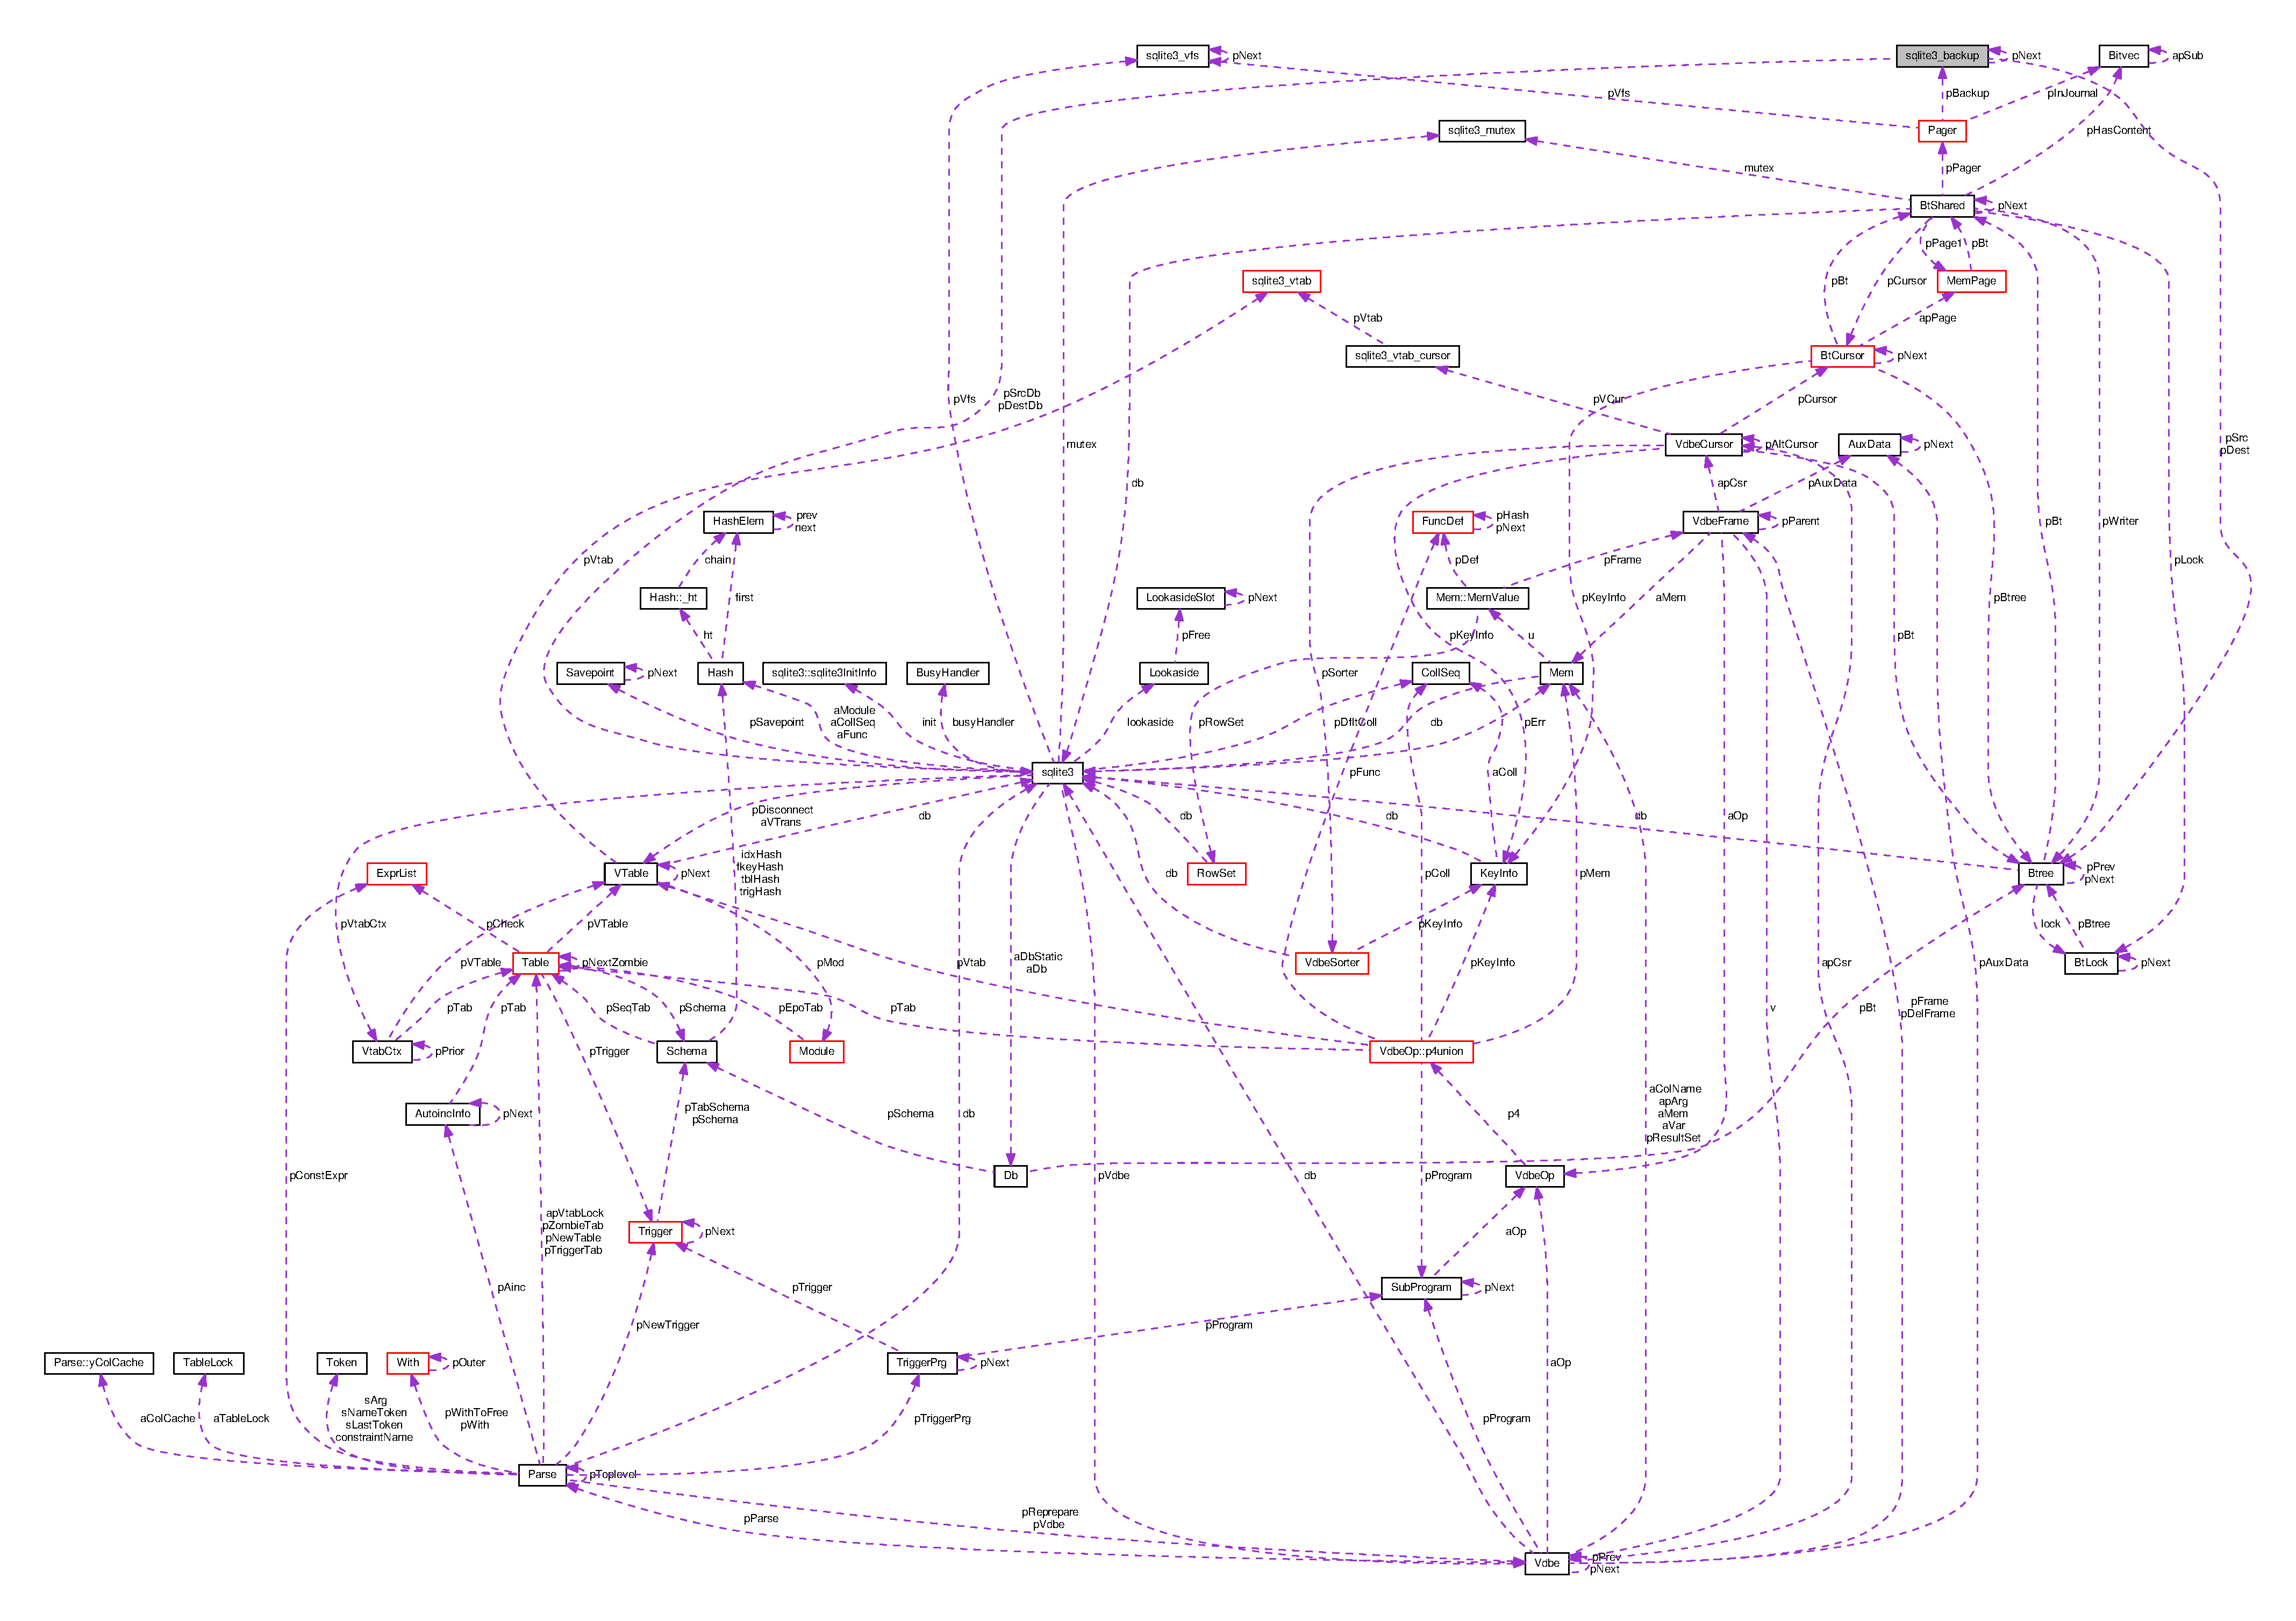
\includegraphics[width=350pt]{structsqlite3__backup__coll__graph}
\end{center}
\end{figure}
\subsection*{Public Attributes}
\begin{DoxyCompactItemize}
\item 
\hyperlink{structsqlite3}{sqlite3} $\ast$ {\bfseries p\+Dest\+Db}\hypertarget{structsqlite3__backup_ad9b5074a860e01b31bbf9cb27f3808d9}{}\label{structsqlite3__backup_ad9b5074a860e01b31bbf9cb27f3808d9}

\item 
\hyperlink{structBtree}{Btree} $\ast$ {\bfseries p\+Dest}\hypertarget{structsqlite3__backup_a9e011336a89274f0ebfefdcede198f71}{}\label{structsqlite3__backup_a9e011336a89274f0ebfefdcede198f71}

\item 
u32 {\bfseries i\+Dest\+Schema}\hypertarget{structsqlite3__backup_a3f294f50b4ef206452dddd14f2a7cf6a}{}\label{structsqlite3__backup_a3f294f50b4ef206452dddd14f2a7cf6a}

\item 
int {\bfseries b\+Dest\+Locked}\hypertarget{structsqlite3__backup_aa0d385678bc5c3fd4da4201ff03a5856}{}\label{structsqlite3__backup_aa0d385678bc5c3fd4da4201ff03a5856}

\item 
Pgno {\bfseries i\+Next}\hypertarget{structsqlite3__backup_a92454bf354f928aade2b2f92e6cfd088}{}\label{structsqlite3__backup_a92454bf354f928aade2b2f92e6cfd088}

\item 
\hyperlink{structsqlite3}{sqlite3} $\ast$ {\bfseries p\+Src\+Db}\hypertarget{structsqlite3__backup_a0bcc0528bb3f5ec52eb40c3e7a4f7adc}{}\label{structsqlite3__backup_a0bcc0528bb3f5ec52eb40c3e7a4f7adc}

\item 
\hyperlink{structBtree}{Btree} $\ast$ {\bfseries p\+Src}\hypertarget{structsqlite3__backup_aa48f873d1de446638ff71fdae606e672}{}\label{structsqlite3__backup_aa48f873d1de446638ff71fdae606e672}

\item 
int {\bfseries rc}\hypertarget{structsqlite3__backup_aab860dbed6181702b4c6b80d43cde411}{}\label{structsqlite3__backup_aab860dbed6181702b4c6b80d43cde411}

\item 
Pgno {\bfseries n\+Remaining}\hypertarget{structsqlite3__backup_a4287faa23d4534e8a33915740604d1e1}{}\label{structsqlite3__backup_a4287faa23d4534e8a33915740604d1e1}

\item 
Pgno {\bfseries n\+Pagecount}\hypertarget{structsqlite3__backup_a98599d5a3a13173a6a126242d1fbbaa8}{}\label{structsqlite3__backup_a98599d5a3a13173a6a126242d1fbbaa8}

\item 
int {\bfseries is\+Attached}\hypertarget{structsqlite3__backup_af515f0d9265847d820cbaad41cef78ae}{}\label{structsqlite3__backup_af515f0d9265847d820cbaad41cef78ae}

\item 
\hyperlink{structsqlite3__backup}{sqlite3\+\_\+backup} $\ast$ {\bfseries p\+Next}\hypertarget{structsqlite3__backup_a3a87332e045fe4a477fe262409c6011a}{}\label{structsqlite3__backup_a3a87332e045fe4a477fe262409c6011a}

\end{DoxyCompactItemize}


The documentation for this struct was generated from the following file\+:\begin{DoxyCompactItemize}
\item 
sqlite3.\+c\end{DoxyCompactItemize}

\hypertarget{structsqlite3__context}{}\section{sqlite3\+\_\+context Struct Reference}
\label{structsqlite3__context}\index{sqlite3\+\_\+context@{sqlite3\+\_\+context}}


Collaboration diagram for sqlite3\+\_\+context\+:
% FIG 0
\subsection*{Public Attributes}
\begin{DoxyCompactItemize}
\item 
\hyperlink{structMem}{Mem} $\ast$ {\bfseries p\+Out}\hypertarget{structsqlite3__context_ae22b1db2ea357b70dda4a86b6df01f34}{}\label{structsqlite3__context_ae22b1db2ea357b70dda4a86b6df01f34}

\item 
\hyperlink{structFuncDef}{Func\+Def} $\ast$ {\bfseries p\+Func}\hypertarget{structsqlite3__context_af4215c87be2c0cb10868f623a552a2aa}{}\label{structsqlite3__context_af4215c87be2c0cb10868f623a552a2aa}

\item 
\hyperlink{structMem}{Mem} $\ast$ {\bfseries p\+Mem}\hypertarget{structsqlite3__context_a7b84aa5920329cb0eb943832175b48b5}{}\label{structsqlite3__context_a7b84aa5920329cb0eb943832175b48b5}

\item 
\hyperlink{structVdbe}{Vdbe} $\ast$ {\bfseries p\+Vdbe}\hypertarget{structsqlite3__context_ab35b02abe9a81e0c8cbdaeb0aa1a5874}{}\label{structsqlite3__context_ab35b02abe9a81e0c8cbdaeb0aa1a5874}

\item 
int {\bfseries i\+Op}\hypertarget{structsqlite3__context_a6f5930106488b9ead6f8efefe9125b6c}{}\label{structsqlite3__context_a6f5930106488b9ead6f8efefe9125b6c}

\item 
int {\bfseries is\+Error}\hypertarget{structsqlite3__context_ae4351b8da8c6d2676074612c1b8d4af5}{}\label{structsqlite3__context_ae4351b8da8c6d2676074612c1b8d4af5}

\item 
u8 {\bfseries skip\+Flag}\hypertarget{structsqlite3__context_a29c404b8744ed5967960c576f3e59bd3}{}\label{structsqlite3__context_a29c404b8744ed5967960c576f3e59bd3}

\item 
u8 {\bfseries f\+Error\+Or\+Aux}\hypertarget{structsqlite3__context_a342986cd1a7c165151c53af83fe24b1d}{}\label{structsqlite3__context_a342986cd1a7c165151c53af83fe24b1d}

\item 
u8 {\bfseries argc}\hypertarget{structsqlite3__context_a3246bd9287c845864193f0519804aede}{}\label{structsqlite3__context_a3246bd9287c845864193f0519804aede}

\item 
\hyperlink{structMem}{sqlite3\+\_\+value} $\ast$ {\bfseries argv} \mbox{[}1\mbox{]}\hypertarget{structsqlite3__context_a416e22362626c80a9dd4c7909871d90c}{}\label{structsqlite3__context_a416e22362626c80a9dd4c7909871d90c}

\end{DoxyCompactItemize}


The documentation for this struct was generated from the following file\+:\begin{DoxyCompactItemize}
\item 
sqlite3.\+c\end{DoxyCompactItemize}

\hypertarget{structsqlite3__file}{}\section{sqlite3\+\_\+file Struct Reference}
\label{structsqlite3__file}\index{sqlite3\+\_\+file@{sqlite3\+\_\+file}}


Collaboration diagram for sqlite3\+\_\+file\+:\nopagebreak
\begin{figure}[H]
\begin{center}
\leavevmode
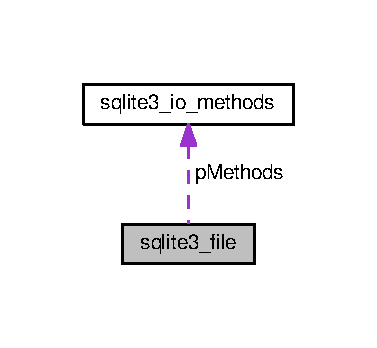
\includegraphics[width=181pt]{structsqlite3__file__coll__graph}
\end{center}
\end{figure}
\subsection*{Public Attributes}
\begin{DoxyCompactItemize}
\item 
const struct \hyperlink{structsqlite3__io__methods}{sqlite3\+\_\+io\+\_\+methods} $\ast$ {\bfseries p\+Methods}\hypertarget{structsqlite3__file_afbe27b40382393e63784a4d4b43f3ad7}{}\label{structsqlite3__file_afbe27b40382393e63784a4d4b43f3ad7}

\end{DoxyCompactItemize}


The documentation for this struct was generated from the following files\+:\begin{DoxyCompactItemize}
\item 
sqlite3.\+c\item 
sqlite3.\+h\end{DoxyCompactItemize}

\hypertarget{structsqlite3__index__info_1_1sqlite3__index__constraint}{}\section{sqlite3\+\_\+index\+\_\+info\+:\+:sqlite3\+\_\+index\+\_\+constraint Struct Reference}
\label{structsqlite3__index__info_1_1sqlite3__index__constraint}\index{sqlite3\+\_\+index\+\_\+info\+::sqlite3\+\_\+index\+\_\+constraint@{sqlite3\+\_\+index\+\_\+info\+::sqlite3\+\_\+index\+\_\+constraint}}
\subsection*{Public Attributes}
\begin{DoxyCompactItemize}
\item 
int {\bfseries i\+Column}\hypertarget{structsqlite3__index__info_1_1sqlite3__index__constraint_a0f1e207060420058ee2881f2ea368e3a}{}\label{structsqlite3__index__info_1_1sqlite3__index__constraint_a0f1e207060420058ee2881f2ea368e3a}

\item 
unsigned char {\bfseries op}\hypertarget{structsqlite3__index__info_1_1sqlite3__index__constraint_a362f4ec1f71975cb0ac39a8b5e4b1476}{}\label{structsqlite3__index__info_1_1sqlite3__index__constraint_a362f4ec1f71975cb0ac39a8b5e4b1476}

\item 
unsigned char {\bfseries usable}\hypertarget{structsqlite3__index__info_1_1sqlite3__index__constraint_ae16e62caeab743cc68bb22227dacb501}{}\label{structsqlite3__index__info_1_1sqlite3__index__constraint_ae16e62caeab743cc68bb22227dacb501}

\item 
int {\bfseries i\+Term\+Offset}\hypertarget{structsqlite3__index__info_1_1sqlite3__index__constraint_a4e8368da66f34b7f07b369984b813d1b}{}\label{structsqlite3__index__info_1_1sqlite3__index__constraint_a4e8368da66f34b7f07b369984b813d1b}

\end{DoxyCompactItemize}


The documentation for this struct was generated from the following files\+:\begin{DoxyCompactItemize}
\item 
sqlite3.\+c\item 
sqlite3.\+h\end{DoxyCompactItemize}

\hypertarget{structsqlite3__index__info_1_1sqlite3__index__constraint__usage}{}\section{sqlite3\+\_\+index\+\_\+info\+:\+:sqlite3\+\_\+index\+\_\+constraint\+\_\+usage Struct Reference}
\label{structsqlite3__index__info_1_1sqlite3__index__constraint__usage}\index{sqlite3\+\_\+index\+\_\+info\+::sqlite3\+\_\+index\+\_\+constraint\+\_\+usage@{sqlite3\+\_\+index\+\_\+info\+::sqlite3\+\_\+index\+\_\+constraint\+\_\+usage}}
\subsection*{Public Attributes}
\begin{DoxyCompactItemize}
\item 
int {\bfseries argv\+Index}\hypertarget{structsqlite3__index__info_1_1sqlite3__index__constraint__usage_a2cbf680033c2937b3de226e091743a94}{}\label{structsqlite3__index__info_1_1sqlite3__index__constraint__usage_a2cbf680033c2937b3de226e091743a94}

\item 
unsigned char {\bfseries omit}\hypertarget{structsqlite3__index__info_1_1sqlite3__index__constraint__usage_ad07fa17d30e4fb3abe23ceaf84edf0ef}{}\label{structsqlite3__index__info_1_1sqlite3__index__constraint__usage_ad07fa17d30e4fb3abe23ceaf84edf0ef}

\end{DoxyCompactItemize}


The documentation for this struct was generated from the following files\+:\begin{DoxyCompactItemize}
\item 
sqlite3.\+c\item 
sqlite3.\+h\end{DoxyCompactItemize}

\hypertarget{structsqlite3__index__info}{}\section{sqlite3\+\_\+index\+\_\+info Struct Reference}
\label{structsqlite3__index__info}\index{sqlite3\+\_\+index\+\_\+info@{sqlite3\+\_\+index\+\_\+info}}


Collaboration diagram for sqlite3\+\_\+index\+\_\+info\+:
% FIG 0
\subsection*{Classes}
\begin{DoxyCompactItemize}
\item 
struct \hyperlink{structsqlite3__index__info_1_1sqlite3__index__constraint}{sqlite3\+\_\+index\+\_\+constraint}
\item 
struct \hyperlink{structsqlite3__index__info_1_1sqlite3__index__constraint__usage}{sqlite3\+\_\+index\+\_\+constraint\+\_\+usage}
\item 
struct \hyperlink{structsqlite3__index__info_1_1sqlite3__index__orderby}{sqlite3\+\_\+index\+\_\+orderby}
\end{DoxyCompactItemize}
\subsection*{Public Attributes}
\begin{DoxyCompactItemize}
\item 
int {\bfseries n\+Constraint}\hypertarget{structsqlite3__index__info_ae861993a30ce914a5214eab2579d935a}{}\label{structsqlite3__index__info_ae861993a30ce914a5214eab2579d935a}

\item 
struct \hyperlink{structsqlite3__index__info_1_1sqlite3__index__constraint}{sqlite3\+\_\+index\+\_\+info\+::sqlite3\+\_\+index\+\_\+constraint} $\ast$ {\bfseries a\+Constraint}\hypertarget{structsqlite3__index__info_a634aa93834e2b47acf34454746c0f248}{}\label{structsqlite3__index__info_a634aa93834e2b47acf34454746c0f248}

\item 
int {\bfseries n\+Order\+By}\hypertarget{structsqlite3__index__info_a3ef850fdc57eddbc8189fe84d0a9044e}{}\label{structsqlite3__index__info_a3ef850fdc57eddbc8189fe84d0a9044e}

\item 
struct \hyperlink{structsqlite3__index__info_1_1sqlite3__index__orderby}{sqlite3\+\_\+index\+\_\+info\+::sqlite3\+\_\+index\+\_\+orderby} $\ast$ {\bfseries a\+Order\+By}\hypertarget{structsqlite3__index__info_a6823a68979e19d8e332389361e920ef9}{}\label{structsqlite3__index__info_a6823a68979e19d8e332389361e920ef9}

\item 
struct \hyperlink{structsqlite3__index__info_1_1sqlite3__index__constraint__usage}{sqlite3\+\_\+index\+\_\+info\+::sqlite3\+\_\+index\+\_\+constraint\+\_\+usage} $\ast$ {\bfseries a\+Constraint\+Usage}\hypertarget{structsqlite3__index__info_a79b8a969dd7d582fc2ea3c0fbc5adb56}{}\label{structsqlite3__index__info_a79b8a969dd7d582fc2ea3c0fbc5adb56}

\item 
int {\bfseries idx\+Num}\hypertarget{structsqlite3__index__info_afcee17707a1c147fbd55c23c807fdae3}{}\label{structsqlite3__index__info_afcee17707a1c147fbd55c23c807fdae3}

\item 
char $\ast$ {\bfseries idx\+Str}\hypertarget{structsqlite3__index__info_ac63f4ebfe8d9331b040fa9e0e47c9d70}{}\label{structsqlite3__index__info_ac63f4ebfe8d9331b040fa9e0e47c9d70}

\item 
int {\bfseries need\+To\+Free\+Idx\+Str}\hypertarget{structsqlite3__index__info_a5410066c067c3891cdf165c70cc4d6b1}{}\label{structsqlite3__index__info_a5410066c067c3891cdf165c70cc4d6b1}

\item 
int {\bfseries order\+By\+Consumed}\hypertarget{structsqlite3__index__info_a5515d9de0f37f68d7e0930c20a668b29}{}\label{structsqlite3__index__info_a5515d9de0f37f68d7e0930c20a668b29}

\item 
double {\bfseries estimated\+Cost}\hypertarget{structsqlite3__index__info_aa8b4fe1d2ee38aab57ba5e1da00d7830}{}\label{structsqlite3__index__info_aa8b4fe1d2ee38aab57ba5e1da00d7830}

\item 
sqlite3\+\_\+int64 {\bfseries estimated\+Rows}\hypertarget{structsqlite3__index__info_adcdf25dcf9848a6fedf539bb9c921b7f}{}\label{structsqlite3__index__info_adcdf25dcf9848a6fedf539bb9c921b7f}

\item 
int {\bfseries idx\+Flags}\hypertarget{structsqlite3__index__info_a8acf2a7efbc3e193cf01d2afbd44fdbb}{}\label{structsqlite3__index__info_a8acf2a7efbc3e193cf01d2afbd44fdbb}

\item 
sqlite3\+\_\+uint64 {\bfseries col\+Used}\hypertarget{structsqlite3__index__info_a99787169e2f78c0728bdb339c4107a2e}{}\label{structsqlite3__index__info_a99787169e2f78c0728bdb339c4107a2e}

\end{DoxyCompactItemize}


The documentation for this struct was generated from the following files\+:\begin{DoxyCompactItemize}
\item 
sqlite3.\+c\item 
sqlite3.\+h\end{DoxyCompactItemize}

\hypertarget{structsqlite3__index__info_1_1sqlite3__index__orderby}{}\section{sqlite3\+\_\+index\+\_\+info\+:\+:sqlite3\+\_\+index\+\_\+orderby Struct Reference}
\label{structsqlite3__index__info_1_1sqlite3__index__orderby}\index{sqlite3\+\_\+index\+\_\+info\+::sqlite3\+\_\+index\+\_\+orderby@{sqlite3\+\_\+index\+\_\+info\+::sqlite3\+\_\+index\+\_\+orderby}}
\subsection*{Public Attributes}
\begin{DoxyCompactItemize}
\item 
int {\bfseries i\+Column}\hypertarget{structsqlite3__index__info_1_1sqlite3__index__orderby_a266396085bfda9acef3f13eaa170cd2f}{}\label{structsqlite3__index__info_1_1sqlite3__index__orderby_a266396085bfda9acef3f13eaa170cd2f}

\item 
unsigned char {\bfseries desc}\hypertarget{structsqlite3__index__info_1_1sqlite3__index__orderby_a0586d1b5d36221af96aeba8cfc56e9c6}{}\label{structsqlite3__index__info_1_1sqlite3__index__orderby_a0586d1b5d36221af96aeba8cfc56e9c6}

\end{DoxyCompactItemize}


The documentation for this struct was generated from the following files\+:\begin{DoxyCompactItemize}
\item 
sqlite3.\+c\item 
sqlite3.\+h\end{DoxyCompactItemize}

\hypertarget{structsqlite3__io__methods}{}\section{sqlite3\+\_\+io\+\_\+methods Struct Reference}
\label{structsqlite3__io__methods}\index{sqlite3\+\_\+io\+\_\+methods@{sqlite3\+\_\+io\+\_\+methods}}
\subsection*{Public Attributes}
\begin{DoxyCompactItemize}
\item 
int {\bfseries i\+Version}\hypertarget{structsqlite3__io__methods_ad1c72bdfde750a09a797f314a096a965}{}\label{structsqlite3__io__methods_ad1c72bdfde750a09a797f314a096a965}

\item 
int($\ast$ {\bfseries x\+Close} )(\hyperlink{structsqlite3__file}{sqlite3\+\_\+file} $\ast$)\hypertarget{structsqlite3__io__methods_a3c021d16959e0533f507b3212681a22e}{}\label{structsqlite3__io__methods_a3c021d16959e0533f507b3212681a22e}

\item 
int($\ast$ {\bfseries x\+Read} )(\hyperlink{structsqlite3__file}{sqlite3\+\_\+file} $\ast$, void $\ast$, int i\+Amt, sqlite3\+\_\+int64 i\+Ofst)\hypertarget{structsqlite3__io__methods_a19870694752f65e8738d89d871d0ca7f}{}\label{structsqlite3__io__methods_a19870694752f65e8738d89d871d0ca7f}

\item 
int($\ast$ {\bfseries x\+Write} )(\hyperlink{structsqlite3__file}{sqlite3\+\_\+file} $\ast$, const void $\ast$, int i\+Amt, sqlite3\+\_\+int64 i\+Ofst)\hypertarget{structsqlite3__io__methods_a803b39bc86bbff522602597fa4390e0f}{}\label{structsqlite3__io__methods_a803b39bc86bbff522602597fa4390e0f}

\item 
int($\ast$ {\bfseries x\+Truncate} )(\hyperlink{structsqlite3__file}{sqlite3\+\_\+file} $\ast$, sqlite3\+\_\+int64 size)\hypertarget{structsqlite3__io__methods_a981cc60fc305bfb38eecd7123a513a20}{}\label{structsqlite3__io__methods_a981cc60fc305bfb38eecd7123a513a20}

\item 
int($\ast$ {\bfseries x\+Sync} )(\hyperlink{structsqlite3__file}{sqlite3\+\_\+file} $\ast$, int flags)\hypertarget{structsqlite3__io__methods_a8d39ac02aeb1eb63622008217031b098}{}\label{structsqlite3__io__methods_a8d39ac02aeb1eb63622008217031b098}

\item 
int($\ast$ {\bfseries x\+File\+Size} )(\hyperlink{structsqlite3__file}{sqlite3\+\_\+file} $\ast$, sqlite3\+\_\+int64 $\ast$p\+Size)\hypertarget{structsqlite3__io__methods_ad269e3cbda39d0a2383aef13b60b02f8}{}\label{structsqlite3__io__methods_ad269e3cbda39d0a2383aef13b60b02f8}

\item 
int($\ast$ {\bfseries x\+Lock} )(\hyperlink{structsqlite3__file}{sqlite3\+\_\+file} $\ast$, int)\hypertarget{structsqlite3__io__methods_a3e4749687788b89ed0f672db7a4f6ac8}{}\label{structsqlite3__io__methods_a3e4749687788b89ed0f672db7a4f6ac8}

\item 
int($\ast$ {\bfseries x\+Unlock} )(\hyperlink{structsqlite3__file}{sqlite3\+\_\+file} $\ast$, int)\hypertarget{structsqlite3__io__methods_ac90eeb9153eb6608a1872760660e718f}{}\label{structsqlite3__io__methods_ac90eeb9153eb6608a1872760660e718f}

\item 
int($\ast$ {\bfseries x\+Check\+Reserved\+Lock} )(\hyperlink{structsqlite3__file}{sqlite3\+\_\+file} $\ast$, int $\ast$p\+Res\+Out)\hypertarget{structsqlite3__io__methods_a97f5eb0c2dc7e1cf2f8ecd6857e4c77c}{}\label{structsqlite3__io__methods_a97f5eb0c2dc7e1cf2f8ecd6857e4c77c}

\item 
int($\ast$ {\bfseries x\+File\+Control} )(\hyperlink{structsqlite3__file}{sqlite3\+\_\+file} $\ast$, int op, void $\ast$p\+Arg)\hypertarget{structsqlite3__io__methods_a5d2a5ba7937b4a6c6c5ba62c4e2b9166}{}\label{structsqlite3__io__methods_a5d2a5ba7937b4a6c6c5ba62c4e2b9166}

\item 
int($\ast$ {\bfseries x\+Sector\+Size} )(\hyperlink{structsqlite3__file}{sqlite3\+\_\+file} $\ast$)\hypertarget{structsqlite3__io__methods_a8436e6eeac404b35057be97f3c2b5c3d}{}\label{structsqlite3__io__methods_a8436e6eeac404b35057be97f3c2b5c3d}

\item 
int($\ast$ {\bfseries x\+Device\+Characteristics} )(\hyperlink{structsqlite3__file}{sqlite3\+\_\+file} $\ast$)\hypertarget{structsqlite3__io__methods_ace5e9e9f267c6c57023109c0658f2683}{}\label{structsqlite3__io__methods_ace5e9e9f267c6c57023109c0658f2683}

\item 
int($\ast$ {\bfseries x\+Shm\+Map} )(\hyperlink{structsqlite3__file}{sqlite3\+\_\+file} $\ast$, int i\+Pg, int pgsz, int, void volatile $\ast$$\ast$)\hypertarget{structsqlite3__io__methods_a42d21006b7f01acb258986f2c090c64d}{}\label{structsqlite3__io__methods_a42d21006b7f01acb258986f2c090c64d}

\item 
int($\ast$ {\bfseries x\+Shm\+Lock} )(\hyperlink{structsqlite3__file}{sqlite3\+\_\+file} $\ast$, int offset, int n, int flags)\hypertarget{structsqlite3__io__methods_a58f4a6b0df86440029cc5fa1b65b1b4e}{}\label{structsqlite3__io__methods_a58f4a6b0df86440029cc5fa1b65b1b4e}

\item 
void($\ast$ {\bfseries x\+Shm\+Barrier} )(\hyperlink{structsqlite3__file}{sqlite3\+\_\+file} $\ast$)\hypertarget{structsqlite3__io__methods_aedf4a59fa25ad33e0625a2aa0f6f2184}{}\label{structsqlite3__io__methods_aedf4a59fa25ad33e0625a2aa0f6f2184}

\item 
int($\ast$ {\bfseries x\+Shm\+Unmap} )(\hyperlink{structsqlite3__file}{sqlite3\+\_\+file} $\ast$, int delete\+Flag)\hypertarget{structsqlite3__io__methods_af69cbc7ece1854576ac262f986871563}{}\label{structsqlite3__io__methods_af69cbc7ece1854576ac262f986871563}

\item 
int($\ast$ {\bfseries x\+Fetch} )(\hyperlink{structsqlite3__file}{sqlite3\+\_\+file} $\ast$, sqlite3\+\_\+int64 i\+Ofst, int i\+Amt, void $\ast$$\ast$pp)\hypertarget{structsqlite3__io__methods_ad817335f15cad777b60d973f73cb542c}{}\label{structsqlite3__io__methods_ad817335f15cad777b60d973f73cb542c}

\item 
int($\ast$ {\bfseries x\+Unfetch} )(\hyperlink{structsqlite3__file}{sqlite3\+\_\+file} $\ast$, sqlite3\+\_\+int64 i\+Ofst, void $\ast$p)\hypertarget{structsqlite3__io__methods_a81c025bf5851547d47ceef8e83214692}{}\label{structsqlite3__io__methods_a81c025bf5851547d47ceef8e83214692}

\end{DoxyCompactItemize}


The documentation for this struct was generated from the following files\+:\begin{DoxyCompactItemize}
\item 
sqlite3.\+c\item 
sqlite3.\+h\end{DoxyCompactItemize}

\hypertarget{structsqlite3__mem__methods}{}\section{sqlite3\+\_\+mem\+\_\+methods Struct Reference}
\label{structsqlite3__mem__methods}\index{sqlite3\+\_\+mem\+\_\+methods@{sqlite3\+\_\+mem\+\_\+methods}}
\subsection*{Public Attributes}
\begin{DoxyCompactItemize}
\item 
void $\ast$($\ast$ {\bfseries x\+Malloc} )(int)\hypertarget{structsqlite3__mem__methods_acb9151cf501c851b61ab6b378832b159}{}\label{structsqlite3__mem__methods_acb9151cf501c851b61ab6b378832b159}

\item 
void($\ast$ {\bfseries x\+Free} )(void $\ast$)\hypertarget{structsqlite3__mem__methods_aa2e7fe8d030adaa17fd23a44fec1eca1}{}\label{structsqlite3__mem__methods_aa2e7fe8d030adaa17fd23a44fec1eca1}

\item 
void $\ast$($\ast$ {\bfseries x\+Realloc} )(void $\ast$, int)\hypertarget{structsqlite3__mem__methods_a5bb7e62164d0934888473c618c61dc77}{}\label{structsqlite3__mem__methods_a5bb7e62164d0934888473c618c61dc77}

\item 
int($\ast$ {\bfseries x\+Size} )(void $\ast$)\hypertarget{structsqlite3__mem__methods_a6c68275b577d66ae659ef30344c8f86c}{}\label{structsqlite3__mem__methods_a6c68275b577d66ae659ef30344c8f86c}

\item 
int($\ast$ {\bfseries x\+Roundup} )(int)\hypertarget{structsqlite3__mem__methods_a8b3f0d1ddeb498c4aaf9bbce5b92a268}{}\label{structsqlite3__mem__methods_a8b3f0d1ddeb498c4aaf9bbce5b92a268}

\item 
int($\ast$ {\bfseries x\+Init} )(void $\ast$)\hypertarget{structsqlite3__mem__methods_ad0997b548928358d655000b6ac825cf4}{}\label{structsqlite3__mem__methods_ad0997b548928358d655000b6ac825cf4}

\item 
void($\ast$ {\bfseries x\+Shutdown} )(void $\ast$)\hypertarget{structsqlite3__mem__methods_a6f48100692bd935d7f3dbb8c701ab6ca}{}\label{structsqlite3__mem__methods_a6f48100692bd935d7f3dbb8c701ab6ca}

\item 
void $\ast$ {\bfseries p\+App\+Data}\hypertarget{structsqlite3__mem__methods_af91b7adfa1f6aace0b129bac800bd444}{}\label{structsqlite3__mem__methods_af91b7adfa1f6aace0b129bac800bd444}

\end{DoxyCompactItemize}


The documentation for this struct was generated from the following files\+:\begin{DoxyCompactItemize}
\item 
sqlite3.\+c\item 
sqlite3.\+h\end{DoxyCompactItemize}

\hypertarget{structsqlite3__module}{}\section{sqlite3\+\_\+module Struct Reference}
\label{structsqlite3__module}\index{sqlite3\+\_\+module@{sqlite3\+\_\+module}}
\subsection*{Public Attributes}
\begin{DoxyCompactItemize}
\item 
int {\bfseries i\+Version}\hypertarget{structsqlite3__module_a42b11d080dc205aea43581b18f925afe}{}\label{structsqlite3__module_a42b11d080dc205aea43581b18f925afe}

\item 
int($\ast$ {\bfseries x\+Create} )(\hyperlink{structsqlite3}{sqlite3} $\ast$, void $\ast$p\+Aux, int argc, const char $\ast$const $\ast$argv, \hyperlink{structsqlite3__vtab}{sqlite3\+\_\+vtab} $\ast$$\ast$pp\+V\+Tab, char $\ast$$\ast$)\hypertarget{structsqlite3__module_a95e327c9d32abd731013395d9e12b8f9}{}\label{structsqlite3__module_a95e327c9d32abd731013395d9e12b8f9}

\item 
int($\ast$ {\bfseries x\+Connect} )(\hyperlink{structsqlite3}{sqlite3} $\ast$, void $\ast$p\+Aux, int argc, const char $\ast$const $\ast$argv, \hyperlink{structsqlite3__vtab}{sqlite3\+\_\+vtab} $\ast$$\ast$pp\+V\+Tab, char $\ast$$\ast$)\hypertarget{structsqlite3__module_acdd9ccc4a6acff230b2d579172ae32d0}{}\label{structsqlite3__module_acdd9ccc4a6acff230b2d579172ae32d0}

\item 
int($\ast$ {\bfseries x\+Best\+Index} )(\hyperlink{structsqlite3__vtab}{sqlite3\+\_\+vtab} $\ast$p\+V\+Tab, \hyperlink{structsqlite3__index__info}{sqlite3\+\_\+index\+\_\+info} $\ast$)\hypertarget{structsqlite3__module_a66577e230ca8de525b30ee6f287eafb1}{}\label{structsqlite3__module_a66577e230ca8de525b30ee6f287eafb1}

\item 
int($\ast$ {\bfseries x\+Disconnect} )(\hyperlink{structsqlite3__vtab}{sqlite3\+\_\+vtab} $\ast$p\+V\+Tab)\hypertarget{structsqlite3__module_a5dbaa6ff075eaff25ccfddaedba06934}{}\label{structsqlite3__module_a5dbaa6ff075eaff25ccfddaedba06934}

\item 
int($\ast$ {\bfseries x\+Destroy} )(\hyperlink{structsqlite3__vtab}{sqlite3\+\_\+vtab} $\ast$p\+V\+Tab)\hypertarget{structsqlite3__module_a296dae8dadd4eb1f7d0f1187650c7aa5}{}\label{structsqlite3__module_a296dae8dadd4eb1f7d0f1187650c7aa5}

\item 
int($\ast$ {\bfseries x\+Open} )(\hyperlink{structsqlite3__vtab}{sqlite3\+\_\+vtab} $\ast$p\+V\+Tab, \hyperlink{structsqlite3__vtab__cursor}{sqlite3\+\_\+vtab\+\_\+cursor} $\ast$$\ast$pp\+Cursor)\hypertarget{structsqlite3__module_a2cb9f8c149617189efa6ceec0a3211e9}{}\label{structsqlite3__module_a2cb9f8c149617189efa6ceec0a3211e9}

\item 
int($\ast$ {\bfseries x\+Close} )(\hyperlink{structsqlite3__vtab__cursor}{sqlite3\+\_\+vtab\+\_\+cursor} $\ast$)\hypertarget{structsqlite3__module_a514c66634a5297ca9879947fa6f8f10f}{}\label{structsqlite3__module_a514c66634a5297ca9879947fa6f8f10f}

\item 
int($\ast$ {\bfseries x\+Filter} )(\hyperlink{structsqlite3__vtab__cursor}{sqlite3\+\_\+vtab\+\_\+cursor} $\ast$, int idx\+Num, const char $\ast$idx\+Str, int argc, \hyperlink{structMem}{sqlite3\+\_\+value} $\ast$$\ast$argv)\hypertarget{structsqlite3__module_a1ddde32dcae461910096ebb2c42d1a6a}{}\label{structsqlite3__module_a1ddde32dcae461910096ebb2c42d1a6a}

\item 
int($\ast$ {\bfseries x\+Next} )(\hyperlink{structsqlite3__vtab__cursor}{sqlite3\+\_\+vtab\+\_\+cursor} $\ast$)\hypertarget{structsqlite3__module_aa739d9a2081db7bf786f1f9fb9d92264}{}\label{structsqlite3__module_aa739d9a2081db7bf786f1f9fb9d92264}

\item 
int($\ast$ {\bfseries x\+Eof} )(\hyperlink{structsqlite3__vtab__cursor}{sqlite3\+\_\+vtab\+\_\+cursor} $\ast$)\hypertarget{structsqlite3__module_ae10cf7d9a7edfecf1daa34a214bf6a64}{}\label{structsqlite3__module_ae10cf7d9a7edfecf1daa34a214bf6a64}

\item 
int($\ast$ {\bfseries x\+Column} )(\hyperlink{structsqlite3__vtab__cursor}{sqlite3\+\_\+vtab\+\_\+cursor} $\ast$, \hyperlink{structsqlite3__context}{sqlite3\+\_\+context} $\ast$, int)\hypertarget{structsqlite3__module_a4c82dc60335ba40c816cdd6c4dce2950}{}\label{structsqlite3__module_a4c82dc60335ba40c816cdd6c4dce2950}

\item 
int($\ast$ {\bfseries x\+Rowid} )(\hyperlink{structsqlite3__vtab__cursor}{sqlite3\+\_\+vtab\+\_\+cursor} $\ast$, sqlite3\+\_\+int64 $\ast$p\+Rowid)\hypertarget{structsqlite3__module_a1e119b28bd3ad706d1982aaa938aac79}{}\label{structsqlite3__module_a1e119b28bd3ad706d1982aaa938aac79}

\item 
int($\ast$ {\bfseries x\+Update} )(\hyperlink{structsqlite3__vtab}{sqlite3\+\_\+vtab} $\ast$, int, \hyperlink{structMem}{sqlite3\+\_\+value} $\ast$$\ast$, sqlite3\+\_\+int64 $\ast$)\hypertarget{structsqlite3__module_a029d0713dbb3c847a6de773a0a179605}{}\label{structsqlite3__module_a029d0713dbb3c847a6de773a0a179605}

\item 
int($\ast$ {\bfseries x\+Begin} )(\hyperlink{structsqlite3__vtab}{sqlite3\+\_\+vtab} $\ast$p\+V\+Tab)\hypertarget{structsqlite3__module_af3ea97df2b110da6ceb4797222e6d86f}{}\label{structsqlite3__module_af3ea97df2b110da6ceb4797222e6d86f}

\item 
int($\ast$ {\bfseries x\+Sync} )(\hyperlink{structsqlite3__vtab}{sqlite3\+\_\+vtab} $\ast$p\+V\+Tab)\hypertarget{structsqlite3__module_a895d78529db2e28e13d1d842512770b6}{}\label{structsqlite3__module_a895d78529db2e28e13d1d842512770b6}

\item 
int($\ast$ {\bfseries x\+Commit} )(\hyperlink{structsqlite3__vtab}{sqlite3\+\_\+vtab} $\ast$p\+V\+Tab)\hypertarget{structsqlite3__module_a465df78231717713e98677c19e60cece}{}\label{structsqlite3__module_a465df78231717713e98677c19e60cece}

\item 
int($\ast$ {\bfseries x\+Rollback} )(\hyperlink{structsqlite3__vtab}{sqlite3\+\_\+vtab} $\ast$p\+V\+Tab)\hypertarget{structsqlite3__module_a3f8676e941a3080557fe10528e04e2f1}{}\label{structsqlite3__module_a3f8676e941a3080557fe10528e04e2f1}

\item 
int($\ast$ {\bfseries x\+Find\+Function} )(\hyperlink{structsqlite3__vtab}{sqlite3\+\_\+vtab} $\ast$p\+Vtab, int n\+Arg, const char $\ast$z\+Name, void($\ast$$\ast$px\+Func)(\hyperlink{structsqlite3__context}{sqlite3\+\_\+context} $\ast$, int, \hyperlink{structMem}{sqlite3\+\_\+value} $\ast$$\ast$), void $\ast$$\ast$pp\+Arg)\hypertarget{structsqlite3__module_ae70a020a7dda960b91943e9f67695dbb}{}\label{structsqlite3__module_ae70a020a7dda960b91943e9f67695dbb}

\item 
int($\ast$ {\bfseries x\+Rename} )(\hyperlink{structsqlite3__vtab}{sqlite3\+\_\+vtab} $\ast$p\+Vtab, const char $\ast$z\+New)\hypertarget{structsqlite3__module_af886782e9a1ea5c4b131b2bc373c8092}{}\label{structsqlite3__module_af886782e9a1ea5c4b131b2bc373c8092}

\item 
int($\ast$ {\bfseries x\+Savepoint} )(\hyperlink{structsqlite3__vtab}{sqlite3\+\_\+vtab} $\ast$p\+V\+Tab, int)\hypertarget{structsqlite3__module_af90f1df803fce1b90048864aeeeee890}{}\label{structsqlite3__module_af90f1df803fce1b90048864aeeeee890}

\item 
int($\ast$ {\bfseries x\+Release} )(\hyperlink{structsqlite3__vtab}{sqlite3\+\_\+vtab} $\ast$p\+V\+Tab, int)\hypertarget{structsqlite3__module_a8dcaa6dc6d9563c8da57e4c8c5055609}{}\label{structsqlite3__module_a8dcaa6dc6d9563c8da57e4c8c5055609}

\item 
int($\ast$ {\bfseries x\+Rollback\+To} )(\hyperlink{structsqlite3__vtab}{sqlite3\+\_\+vtab} $\ast$p\+V\+Tab, int)\hypertarget{structsqlite3__module_a767753c6c97d1f622e5113367a0547b5}{}\label{structsqlite3__module_a767753c6c97d1f622e5113367a0547b5}

\end{DoxyCompactItemize}


The documentation for this struct was generated from the following files\+:\begin{DoxyCompactItemize}
\item 
sqlite3.\+c\item 
sqlite3.\+h\end{DoxyCompactItemize}

\hypertarget{structsqlite3__mutex}{}\section{sqlite3\+\_\+mutex Struct Reference}
\label{structsqlite3__mutex}\index{sqlite3\+\_\+mutex@{sqlite3\+\_\+mutex}}
\subsection*{Public Attributes}
\begin{DoxyCompactItemize}
\item 
pthread\+\_\+mutex\+\_\+t {\bfseries mutex}\hypertarget{structsqlite3__mutex_a6eef25bee73a3640dbbd052d707dbfdc}{}\label{structsqlite3__mutex_a6eef25bee73a3640dbbd052d707dbfdc}

\end{DoxyCompactItemize}


The documentation for this struct was generated from the following file\+:\begin{DoxyCompactItemize}
\item 
sqlite3.\+c\end{DoxyCompactItemize}

\hypertarget{structsqlite3__mutex__methods}{}\section{sqlite3\+\_\+mutex\+\_\+methods Struct Reference}
\label{structsqlite3__mutex__methods}\index{sqlite3\+\_\+mutex\+\_\+methods@{sqlite3\+\_\+mutex\+\_\+methods}}


Collaboration diagram for sqlite3\+\_\+mutex\+\_\+methods\+:
% FIG 0
\subsection*{Public Attributes}
\begin{DoxyCompactItemize}
\item 
int($\ast$ {\bfseries x\+Mutex\+Init} )(void)\hypertarget{structsqlite3__mutex__methods_af0a78d79b6029444d4a2ac7c474030d4}{}\label{structsqlite3__mutex__methods_af0a78d79b6029444d4a2ac7c474030d4}

\item 
int($\ast$ {\bfseries x\+Mutex\+End} )(void)\hypertarget{structsqlite3__mutex__methods_a4963efb4bfede244d4d2a14510dbfe68}{}\label{structsqlite3__mutex__methods_a4963efb4bfede244d4d2a14510dbfe68}

\item 
\hyperlink{structsqlite3__mutex}{sqlite3\+\_\+mutex} $\ast$($\ast$ {\bfseries x\+Mutex\+Alloc} )(int)\hypertarget{structsqlite3__mutex__methods_a1092d5c1659c494c5235e884def5e275}{}\label{structsqlite3__mutex__methods_a1092d5c1659c494c5235e884def5e275}

\item 
void($\ast$ {\bfseries x\+Mutex\+Free} )(\hyperlink{structsqlite3__mutex}{sqlite3\+\_\+mutex} $\ast$)\hypertarget{structsqlite3__mutex__methods_a4e58d446a7225ce91073eb0af91d219a}{}\label{structsqlite3__mutex__methods_a4e58d446a7225ce91073eb0af91d219a}

\item 
void($\ast$ {\bfseries x\+Mutex\+Enter} )(\hyperlink{structsqlite3__mutex}{sqlite3\+\_\+mutex} $\ast$)\hypertarget{structsqlite3__mutex__methods_ac60f7bb165e9770949a8a2b2c2632830}{}\label{structsqlite3__mutex__methods_ac60f7bb165e9770949a8a2b2c2632830}

\item 
int($\ast$ {\bfseries x\+Mutex\+Try} )(\hyperlink{structsqlite3__mutex}{sqlite3\+\_\+mutex} $\ast$)\hypertarget{structsqlite3__mutex__methods_a45682df41bdfcb267a696090c80ebd06}{}\label{structsqlite3__mutex__methods_a45682df41bdfcb267a696090c80ebd06}

\item 
void($\ast$ {\bfseries x\+Mutex\+Leave} )(\hyperlink{structsqlite3__mutex}{sqlite3\+\_\+mutex} $\ast$)\hypertarget{structsqlite3__mutex__methods_acfa193f9130bfc68caf7f1849bcd0dac}{}\label{structsqlite3__mutex__methods_acfa193f9130bfc68caf7f1849bcd0dac}

\item 
int($\ast$ {\bfseries x\+Mutex\+Held} )(\hyperlink{structsqlite3__mutex}{sqlite3\+\_\+mutex} $\ast$)\hypertarget{structsqlite3__mutex__methods_a5d30a95c614bc08fe156c9ea0f0d88e8}{}\label{structsqlite3__mutex__methods_a5d30a95c614bc08fe156c9ea0f0d88e8}

\item 
int($\ast$ {\bfseries x\+Mutex\+Notheld} )(\hyperlink{structsqlite3__mutex}{sqlite3\+\_\+mutex} $\ast$)\hypertarget{structsqlite3__mutex__methods_a7bc1edfd01c67c6dcee26299bc31a7bf}{}\label{structsqlite3__mutex__methods_a7bc1edfd01c67c6dcee26299bc31a7bf}

\end{DoxyCompactItemize}


The documentation for this struct was generated from the following files\+:\begin{DoxyCompactItemize}
\item 
sqlite3.\+c\item 
sqlite3.\+h\end{DoxyCompactItemize}

\hypertarget{structsqlite3__pcache__methods}{}\section{sqlite3\+\_\+pcache\+\_\+methods Struct Reference}
\label{structsqlite3__pcache__methods}\index{sqlite3\+\_\+pcache\+\_\+methods@{sqlite3\+\_\+pcache\+\_\+methods}}
\subsection*{Public Attributes}
\begin{DoxyCompactItemize}
\item 
void $\ast$ {\bfseries p\+Arg}\hypertarget{structsqlite3__pcache__methods_a90394a920f6a09dd13553aeb79bbed88}{}\label{structsqlite3__pcache__methods_a90394a920f6a09dd13553aeb79bbed88}

\item 
int($\ast$ {\bfseries x\+Init} )(void $\ast$)\hypertarget{structsqlite3__pcache__methods_ab5f54101f6060de1af0c87b2456231ad}{}\label{structsqlite3__pcache__methods_ab5f54101f6060de1af0c87b2456231ad}

\item 
void($\ast$ {\bfseries x\+Shutdown} )(void $\ast$)\hypertarget{structsqlite3__pcache__methods_aa88bb238d288631e7e06f4da232c3dbb}{}\label{structsqlite3__pcache__methods_aa88bb238d288631e7e06f4da232c3dbb}

\item 
sqlite3\+\_\+pcache $\ast$($\ast$ {\bfseries x\+Create} )(int sz\+Page, int b\+Purgeable)\hypertarget{structsqlite3__pcache__methods_a36b1da95aeb7972c3c0d358aedf2a3d4}{}\label{structsqlite3__pcache__methods_a36b1da95aeb7972c3c0d358aedf2a3d4}

\item 
void($\ast$ {\bfseries x\+Cachesize} )(sqlite3\+\_\+pcache $\ast$, int n\+Cachesize)\hypertarget{structsqlite3__pcache__methods_a9cf385dbec7f0d19793e2616a73a3b7f}{}\label{structsqlite3__pcache__methods_a9cf385dbec7f0d19793e2616a73a3b7f}

\item 
int($\ast$ {\bfseries x\+Pagecount} )(sqlite3\+\_\+pcache $\ast$)\hypertarget{structsqlite3__pcache__methods_a0ab192dc811798e8f17c445dbf379989}{}\label{structsqlite3__pcache__methods_a0ab192dc811798e8f17c445dbf379989}

\item 
void $\ast$($\ast$ {\bfseries x\+Fetch} )(sqlite3\+\_\+pcache $\ast$, unsigned key, int create\+Flag)\hypertarget{structsqlite3__pcache__methods_a2e054ad70c9672b504d3d7291e4eb487}{}\label{structsqlite3__pcache__methods_a2e054ad70c9672b504d3d7291e4eb487}

\item 
void($\ast$ {\bfseries x\+Unpin} )(sqlite3\+\_\+pcache $\ast$, void $\ast$, int discard)\hypertarget{structsqlite3__pcache__methods_ade2ab50cc6896be03ee86541877fa85e}{}\label{structsqlite3__pcache__methods_ade2ab50cc6896be03ee86541877fa85e}

\item 
void($\ast$ {\bfseries x\+Rekey} )(sqlite3\+\_\+pcache $\ast$, void $\ast$, unsigned old\+Key, unsigned new\+Key)\hypertarget{structsqlite3__pcache__methods_adc5552190f1de86eb95d91e9cf8430e6}{}\label{structsqlite3__pcache__methods_adc5552190f1de86eb95d91e9cf8430e6}

\item 
void($\ast$ {\bfseries x\+Truncate} )(sqlite3\+\_\+pcache $\ast$, unsigned i\+Limit)\hypertarget{structsqlite3__pcache__methods_aad73f9335999770bcd2dc6a2d914b4f0}{}\label{structsqlite3__pcache__methods_aad73f9335999770bcd2dc6a2d914b4f0}

\item 
void($\ast$ {\bfseries x\+Destroy} )(sqlite3\+\_\+pcache $\ast$)\hypertarget{structsqlite3__pcache__methods_aac18fc581d8d63550a6657016c24ba5d}{}\label{structsqlite3__pcache__methods_aac18fc581d8d63550a6657016c24ba5d}

\end{DoxyCompactItemize}


The documentation for this struct was generated from the following files\+:\begin{DoxyCompactItemize}
\item 
sqlite3.\+c\item 
sqlite3.\+h\end{DoxyCompactItemize}

\hypertarget{structsqlite3__pcache__methods2}{}\section{sqlite3\+\_\+pcache\+\_\+methods2 Struct Reference}
\label{structsqlite3__pcache__methods2}\index{sqlite3\+\_\+pcache\+\_\+methods2@{sqlite3\+\_\+pcache\+\_\+methods2}}


Collaboration diagram for sqlite3\+\_\+pcache\+\_\+methods2\+:\nopagebreak
\begin{figure}[H]
\begin{center}
\leavevmode
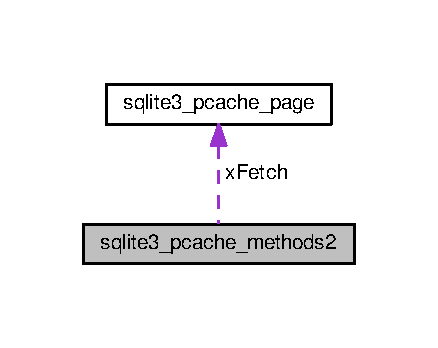
\includegraphics[width=210pt]{structsqlite3__pcache__methods2__coll__graph}
\end{center}
\end{figure}
\subsection*{Public Attributes}
\begin{DoxyCompactItemize}
\item 
int {\bfseries i\+Version}\hypertarget{structsqlite3__pcache__methods2_a03b27be6c7cb8f1d2662c454cbe58483}{}\label{structsqlite3__pcache__methods2_a03b27be6c7cb8f1d2662c454cbe58483}

\item 
void $\ast$ {\bfseries p\+Arg}\hypertarget{structsqlite3__pcache__methods2_a4bea91c33987eef02122bbf8a49745de}{}\label{structsqlite3__pcache__methods2_a4bea91c33987eef02122bbf8a49745de}

\item 
int($\ast$ {\bfseries x\+Init} )(void $\ast$)\hypertarget{structsqlite3__pcache__methods2_a8f77114458576c9d75cd53822fcd3462}{}\label{structsqlite3__pcache__methods2_a8f77114458576c9d75cd53822fcd3462}

\item 
void($\ast$ {\bfseries x\+Shutdown} )(void $\ast$)\hypertarget{structsqlite3__pcache__methods2_a00a780e295b89976940cd3cba2cfeaee}{}\label{structsqlite3__pcache__methods2_a00a780e295b89976940cd3cba2cfeaee}

\item 
sqlite3\+\_\+pcache $\ast$($\ast$ {\bfseries x\+Create} )(int sz\+Page, int sz\+Extra, int b\+Purgeable)\hypertarget{structsqlite3__pcache__methods2_a91e7752b826e19e7c51c1fa0ce530f0f}{}\label{structsqlite3__pcache__methods2_a91e7752b826e19e7c51c1fa0ce530f0f}

\item 
void($\ast$ {\bfseries x\+Cachesize} )(sqlite3\+\_\+pcache $\ast$, int n\+Cachesize)\hypertarget{structsqlite3__pcache__methods2_a4889ab0903938f485aa0fa4fc6925d26}{}\label{structsqlite3__pcache__methods2_a4889ab0903938f485aa0fa4fc6925d26}

\item 
int($\ast$ {\bfseries x\+Pagecount} )(sqlite3\+\_\+pcache $\ast$)\hypertarget{structsqlite3__pcache__methods2_a5d51aba3927db1da9acf31fbdf7d57b5}{}\label{structsqlite3__pcache__methods2_a5d51aba3927db1da9acf31fbdf7d57b5}

\item 
\hyperlink{structsqlite3__pcache__page}{sqlite3\+\_\+pcache\+\_\+page} $\ast$($\ast$ {\bfseries x\+Fetch} )(sqlite3\+\_\+pcache $\ast$, unsigned key, int create\+Flag)\hypertarget{structsqlite3__pcache__methods2_ac74dd2b35193a4309494311995da2d25}{}\label{structsqlite3__pcache__methods2_ac74dd2b35193a4309494311995da2d25}

\item 
void($\ast$ {\bfseries x\+Unpin} )(sqlite3\+\_\+pcache $\ast$, \hyperlink{structsqlite3__pcache__page}{sqlite3\+\_\+pcache\+\_\+page} $\ast$, int discard)\hypertarget{structsqlite3__pcache__methods2_ac94294551eda282f17b1ed2a110e1850}{}\label{structsqlite3__pcache__methods2_ac94294551eda282f17b1ed2a110e1850}

\item 
void($\ast$ {\bfseries x\+Rekey} )(sqlite3\+\_\+pcache $\ast$, \hyperlink{structsqlite3__pcache__page}{sqlite3\+\_\+pcache\+\_\+page} $\ast$, unsigned old\+Key, unsigned new\+Key)\hypertarget{structsqlite3__pcache__methods2_a28a22927b108182e22025bbe6ba1f68e}{}\label{structsqlite3__pcache__methods2_a28a22927b108182e22025bbe6ba1f68e}

\item 
void($\ast$ {\bfseries x\+Truncate} )(sqlite3\+\_\+pcache $\ast$, unsigned i\+Limit)\hypertarget{structsqlite3__pcache__methods2_a7c565709ab91dbe7feb5b82c684ba604}{}\label{structsqlite3__pcache__methods2_a7c565709ab91dbe7feb5b82c684ba604}

\item 
void($\ast$ {\bfseries x\+Destroy} )(sqlite3\+\_\+pcache $\ast$)\hypertarget{structsqlite3__pcache__methods2_a144d6e899889e80e00f93fb6c83359e2}{}\label{structsqlite3__pcache__methods2_a144d6e899889e80e00f93fb6c83359e2}

\item 
void($\ast$ {\bfseries x\+Shrink} )(sqlite3\+\_\+pcache $\ast$)\hypertarget{structsqlite3__pcache__methods2_af00c121e9c39b1df292711013c226ba5}{}\label{structsqlite3__pcache__methods2_af00c121e9c39b1df292711013c226ba5}

\end{DoxyCompactItemize}


The documentation for this struct was generated from the following files\+:\begin{DoxyCompactItemize}
\item 
sqlite3.\+c\item 
sqlite3.\+h\end{DoxyCompactItemize}

\hypertarget{structsqlite3__pcache__page}{}\section{sqlite3\+\_\+pcache\+\_\+page Struct Reference}
\label{structsqlite3__pcache__page}\index{sqlite3\+\_\+pcache\+\_\+page@{sqlite3\+\_\+pcache\+\_\+page}}
\subsection*{Public Attributes}
\begin{DoxyCompactItemize}
\item 
void $\ast$ {\bfseries p\+Buf}\hypertarget{structsqlite3__pcache__page_aa5446325077c05e4b242c8e2d0faba3b}{}\label{structsqlite3__pcache__page_aa5446325077c05e4b242c8e2d0faba3b}

\item 
void $\ast$ {\bfseries p\+Extra}\hypertarget{structsqlite3__pcache__page_a96d7b0314d02837dd6a5e7057912f74f}{}\label{structsqlite3__pcache__page_a96d7b0314d02837dd6a5e7057912f74f}

\end{DoxyCompactItemize}


The documentation for this struct was generated from the following files\+:\begin{DoxyCompactItemize}
\item 
sqlite3.\+c\item 
sqlite3.\+h\end{DoxyCompactItemize}

\hypertarget{structsqlite3__rtree__geometry}{}\section{sqlite3\+\_\+rtree\+\_\+geometry Struct Reference}
\label{structsqlite3__rtree__geometry}\index{sqlite3\+\_\+rtree\+\_\+geometry@{sqlite3\+\_\+rtree\+\_\+geometry}}
\subsection*{Public Attributes}
\begin{DoxyCompactItemize}
\item 
void $\ast$ {\bfseries p\+Context}\hypertarget{structsqlite3__rtree__geometry_a33f98691626846c1317419654d5c5f51}{}\label{structsqlite3__rtree__geometry_a33f98691626846c1317419654d5c5f51}

\item 
int {\bfseries n\+Param}\hypertarget{structsqlite3__rtree__geometry_ada7b9eba82660e3321dd4c93526697c9}{}\label{structsqlite3__rtree__geometry_ada7b9eba82660e3321dd4c93526697c9}

\item 
sqlite3\+\_\+rtree\+\_\+dbl $\ast$ {\bfseries a\+Param}\hypertarget{structsqlite3__rtree__geometry_a42eafbc0dcb02ed32a0a4b10ff887416}{}\label{structsqlite3__rtree__geometry_a42eafbc0dcb02ed32a0a4b10ff887416}

\item 
void $\ast$ {\bfseries p\+User}\hypertarget{structsqlite3__rtree__geometry_a6fdedfd741cf5055f9562298cd32dc74}{}\label{structsqlite3__rtree__geometry_a6fdedfd741cf5055f9562298cd32dc74}

\item 
void($\ast$ {\bfseries x\+Del\+User} )(void $\ast$)\hypertarget{structsqlite3__rtree__geometry_afa1ed10f488b306df354efe56efdf287}{}\label{structsqlite3__rtree__geometry_afa1ed10f488b306df354efe56efdf287}

\end{DoxyCompactItemize}


The documentation for this struct was generated from the following files\+:\begin{DoxyCompactItemize}
\item 
sqlite3.\+c\item 
sqlite3.\+h\end{DoxyCompactItemize}

\hypertarget{structsqlite3__rtree__query__info}{}\section{sqlite3\+\_\+rtree\+\_\+query\+\_\+info Struct Reference}
\label{structsqlite3__rtree__query__info}\index{sqlite3\+\_\+rtree\+\_\+query\+\_\+info@{sqlite3\+\_\+rtree\+\_\+query\+\_\+info}}


Collaboration diagram for sqlite3\+\_\+rtree\+\_\+query\+\_\+info\+:\nopagebreak
\begin{figure}[H]
\begin{center}
\leavevmode
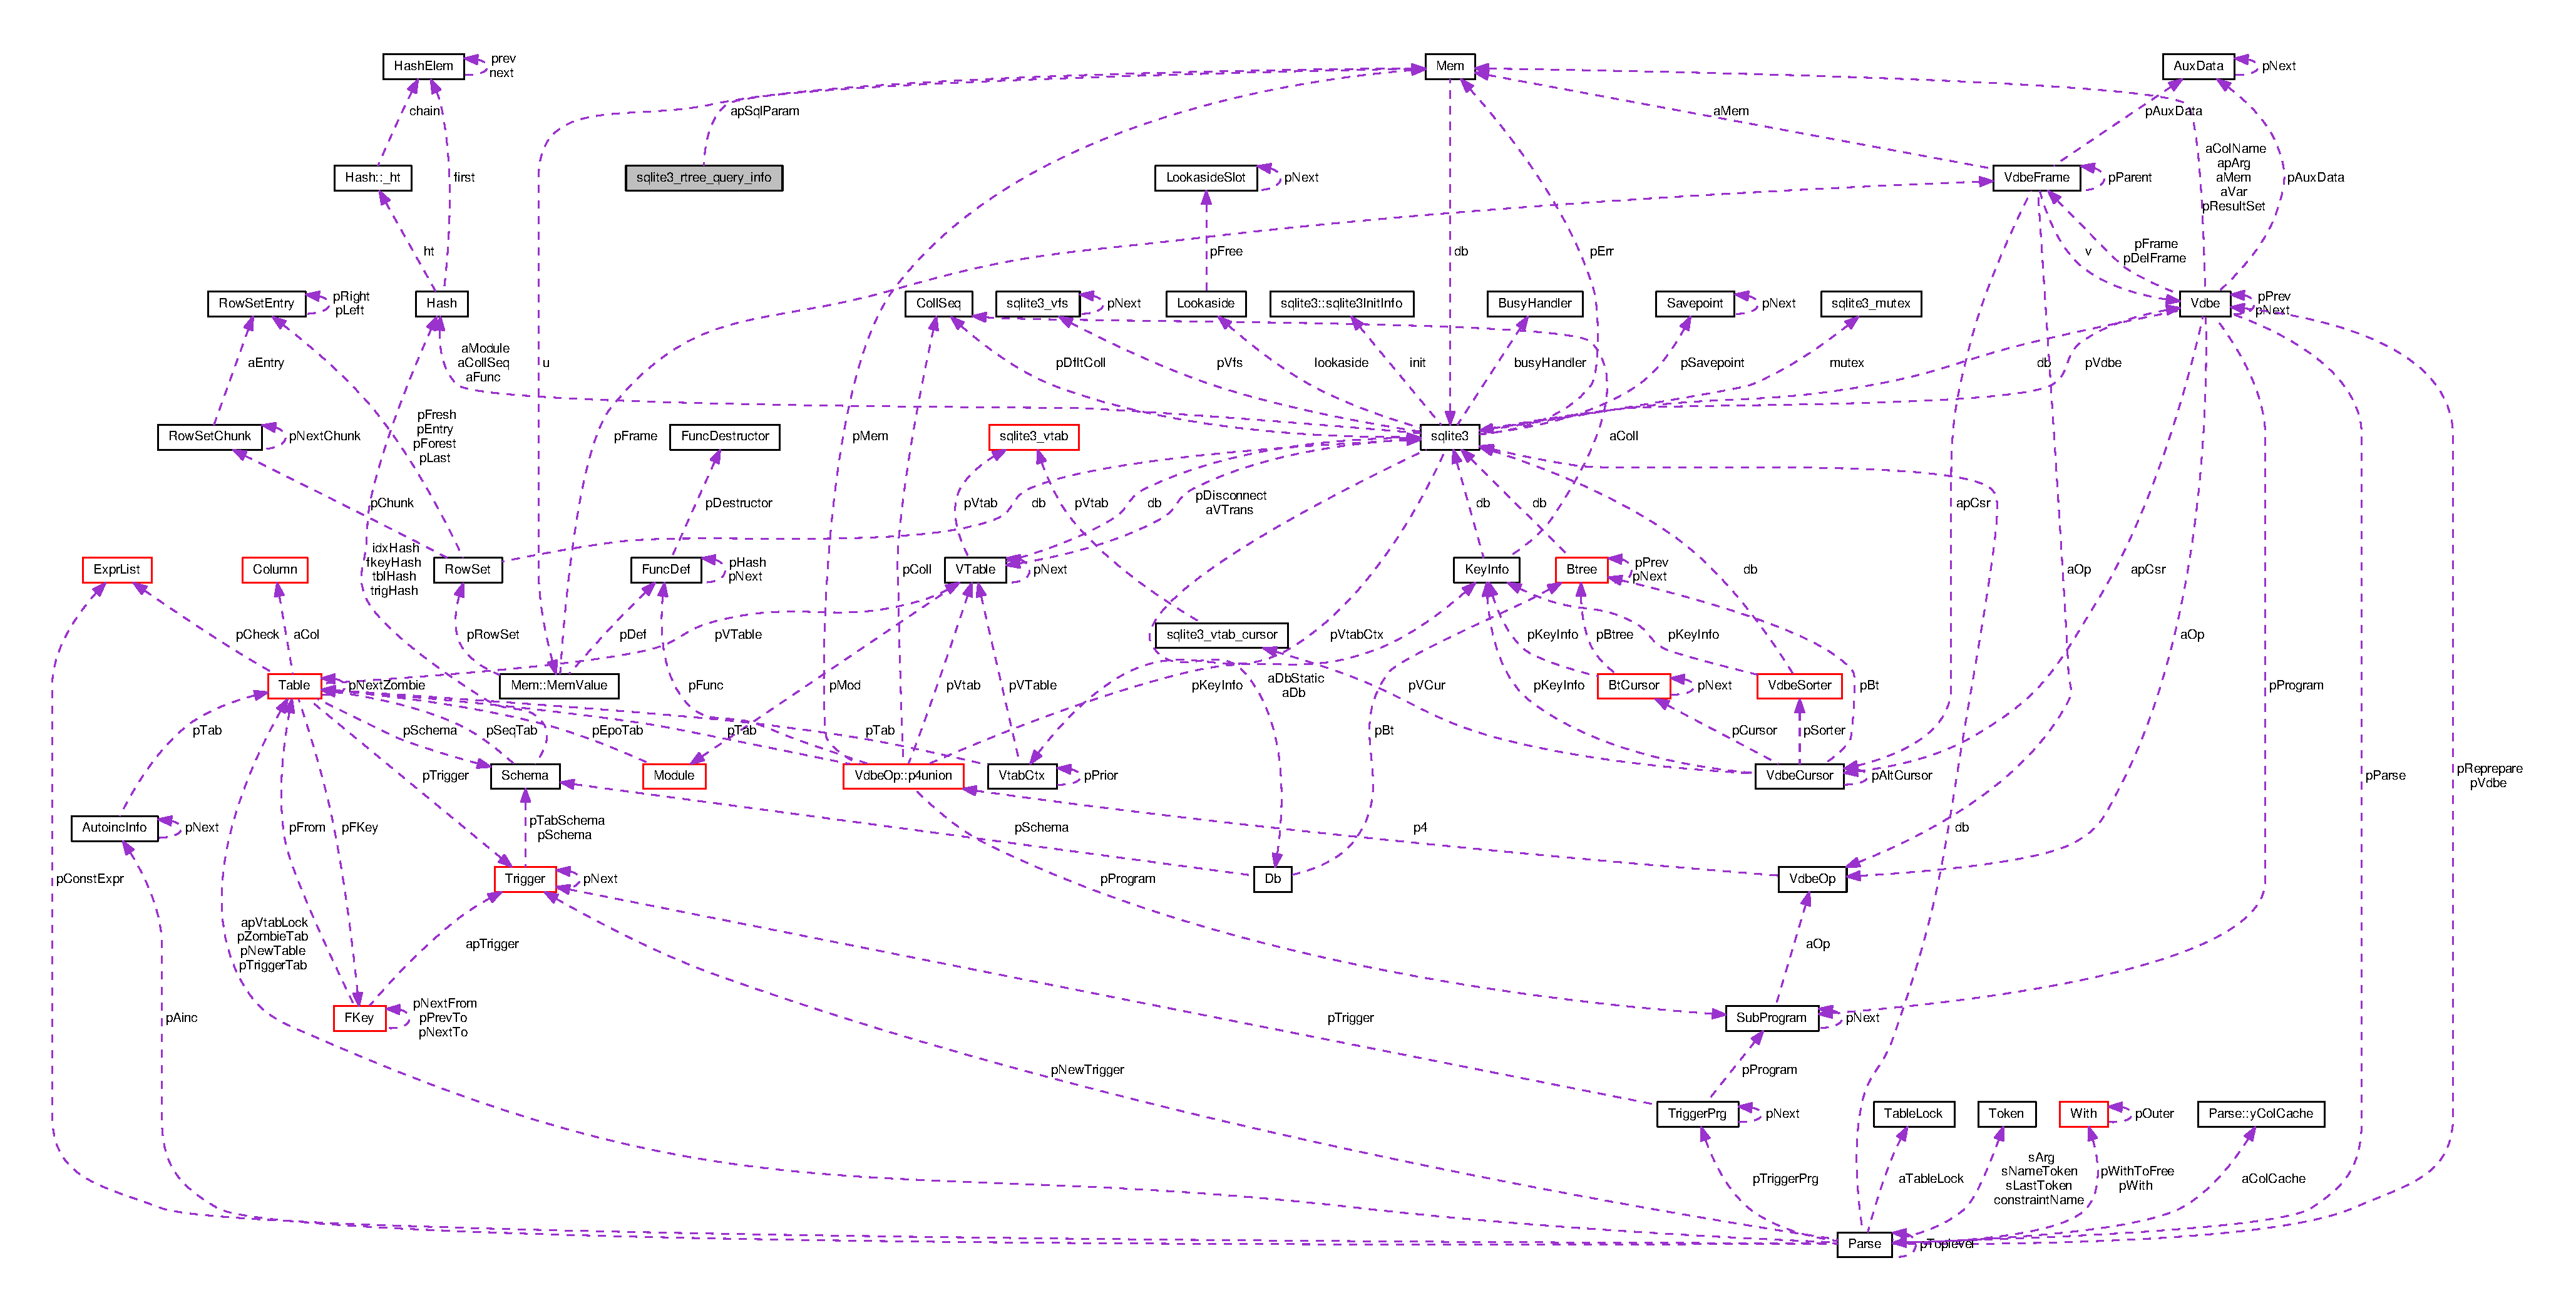
\includegraphics[width=350pt]{structsqlite3__rtree__query__info__coll__graph}
\end{center}
\end{figure}
\subsection*{Public Attributes}
\begin{DoxyCompactItemize}
\item 
void $\ast$ {\bfseries p\+Context}\hypertarget{structsqlite3__rtree__query__info_a7b6167ce5f7bbccffbfa1c57bf5a29d9}{}\label{structsqlite3__rtree__query__info_a7b6167ce5f7bbccffbfa1c57bf5a29d9}

\item 
int {\bfseries n\+Param}\hypertarget{structsqlite3__rtree__query__info_a9df4acb109f572455c8e2fb443027157}{}\label{structsqlite3__rtree__query__info_a9df4acb109f572455c8e2fb443027157}

\item 
sqlite3\+\_\+rtree\+\_\+dbl $\ast$ {\bfseries a\+Param}\hypertarget{structsqlite3__rtree__query__info_a8dec761b0488860396c021a5d1ca079f}{}\label{structsqlite3__rtree__query__info_a8dec761b0488860396c021a5d1ca079f}

\item 
void $\ast$ {\bfseries p\+User}\hypertarget{structsqlite3__rtree__query__info_a194519db635c0afe0667a25eafe35fdc}{}\label{structsqlite3__rtree__query__info_a194519db635c0afe0667a25eafe35fdc}

\item 
void($\ast$ {\bfseries x\+Del\+User} )(void $\ast$)\hypertarget{structsqlite3__rtree__query__info_a316a86ba7544e9388646fdd960052cd2}{}\label{structsqlite3__rtree__query__info_a316a86ba7544e9388646fdd960052cd2}

\item 
sqlite3\+\_\+rtree\+\_\+dbl $\ast$ {\bfseries a\+Coord}\hypertarget{structsqlite3__rtree__query__info_a25340b0dbf1d566172da1d71a4db1427}{}\label{structsqlite3__rtree__query__info_a25340b0dbf1d566172da1d71a4db1427}

\item 
unsigned int $\ast$ {\bfseries an\+Queue}\hypertarget{structsqlite3__rtree__query__info_a7ce9664e95ce7255b87d948986e311c9}{}\label{structsqlite3__rtree__query__info_a7ce9664e95ce7255b87d948986e311c9}

\item 
int {\bfseries n\+Coord}\hypertarget{structsqlite3__rtree__query__info_aa4b95a36fe7306e17e8cf9329fcb0964}{}\label{structsqlite3__rtree__query__info_aa4b95a36fe7306e17e8cf9329fcb0964}

\item 
int {\bfseries i\+Level}\hypertarget{structsqlite3__rtree__query__info_af91ca2d5f867b3b0aa9c91920a3b5b45}{}\label{structsqlite3__rtree__query__info_af91ca2d5f867b3b0aa9c91920a3b5b45}

\item 
int {\bfseries mx\+Level}\hypertarget{structsqlite3__rtree__query__info_ac84533734fb4c86c3f2deba904118785}{}\label{structsqlite3__rtree__query__info_ac84533734fb4c86c3f2deba904118785}

\item 
sqlite3\+\_\+int64 {\bfseries i\+Rowid}\hypertarget{structsqlite3__rtree__query__info_a9e43489993c8aeace851f86eaa00ec26}{}\label{structsqlite3__rtree__query__info_a9e43489993c8aeace851f86eaa00ec26}

\item 
sqlite3\+\_\+rtree\+\_\+dbl {\bfseries r\+Parent\+Score}\hypertarget{structsqlite3__rtree__query__info_af7da93e7fc405eec7e7ec90ab237eab2}{}\label{structsqlite3__rtree__query__info_af7da93e7fc405eec7e7ec90ab237eab2}

\item 
int {\bfseries e\+Parent\+Within}\hypertarget{structsqlite3__rtree__query__info_a8bd37c6af5427c35830f674a4db682c3}{}\label{structsqlite3__rtree__query__info_a8bd37c6af5427c35830f674a4db682c3}

\item 
int {\bfseries e\+Within}\hypertarget{structsqlite3__rtree__query__info_ad1038309f7ea55472a7ff99bf4f9d514}{}\label{structsqlite3__rtree__query__info_ad1038309f7ea55472a7ff99bf4f9d514}

\item 
sqlite3\+\_\+rtree\+\_\+dbl {\bfseries r\+Score}\hypertarget{structsqlite3__rtree__query__info_af449e4a3607573d17b3d31c67b6e1584}{}\label{structsqlite3__rtree__query__info_af449e4a3607573d17b3d31c67b6e1584}

\item 
\hyperlink{structMem}{sqlite3\+\_\+value} $\ast$$\ast$ {\bfseries ap\+Sql\+Param}\hypertarget{structsqlite3__rtree__query__info_a91c604c985d05e67f08b7370d7bf92aa}{}\label{structsqlite3__rtree__query__info_a91c604c985d05e67f08b7370d7bf92aa}

\end{DoxyCompactItemize}


The documentation for this struct was generated from the following files\+:\begin{DoxyCompactItemize}
\item 
sqlite3.\+c\item 
sqlite3.\+h\end{DoxyCompactItemize}

\hypertarget{structsqlite3__vfs}{}\section{sqlite3\+\_\+vfs Struct Reference}
\label{structsqlite3__vfs}\index{sqlite3\+\_\+vfs@{sqlite3\+\_\+vfs}}


Collaboration diagram for sqlite3\+\_\+vfs\+:\nopagebreak
\begin{figure}[H]
\begin{center}
\leavevmode
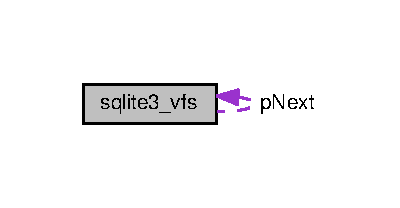
\includegraphics[width=192pt]{structsqlite3__vfs__coll__graph}
\end{center}
\end{figure}
\subsection*{Public Attributes}
\begin{DoxyCompactItemize}
\item 
int {\bfseries i\+Version}\hypertarget{structsqlite3__vfs_a694dd264949bd163545fe174510ed019}{}\label{structsqlite3__vfs_a694dd264949bd163545fe174510ed019}

\item 
int {\bfseries sz\+Os\+File}\hypertarget{structsqlite3__vfs_a549399081342d61134b6398562a0a997}{}\label{structsqlite3__vfs_a549399081342d61134b6398562a0a997}

\item 
int {\bfseries mx\+Pathname}\hypertarget{structsqlite3__vfs_adb2d82c74891b00b5529fb94e7710135}{}\label{structsqlite3__vfs_adb2d82c74891b00b5529fb94e7710135}

\item 
\hyperlink{structsqlite3__vfs}{sqlite3\+\_\+vfs} $\ast$ {\bfseries p\+Next}\hypertarget{structsqlite3__vfs_a4b12c503e4083854a9c4d91697a12de3}{}\label{structsqlite3__vfs_a4b12c503e4083854a9c4d91697a12de3}

\item 
const char $\ast$ {\bfseries z\+Name}\hypertarget{structsqlite3__vfs_a01a82d3e1a7efc00a762a00751ed592b}{}\label{structsqlite3__vfs_a01a82d3e1a7efc00a762a00751ed592b}

\item 
void $\ast$ {\bfseries p\+App\+Data}\hypertarget{structsqlite3__vfs_a8de686c5e679ba421479ac96d6654527}{}\label{structsqlite3__vfs_a8de686c5e679ba421479ac96d6654527}

\item 
int($\ast$ {\bfseries x\+Open} )(\hyperlink{structsqlite3__vfs}{sqlite3\+\_\+vfs} $\ast$, const char $\ast$z\+Name, \hyperlink{structsqlite3__file}{sqlite3\+\_\+file} $\ast$, int flags, int $\ast$p\+Out\+Flags)\hypertarget{structsqlite3__vfs_a5f35d5528d8fdf1d26e1e206879afbe1}{}\label{structsqlite3__vfs_a5f35d5528d8fdf1d26e1e206879afbe1}

\item 
int($\ast$ {\bfseries x\+Delete} )(\hyperlink{structsqlite3__vfs}{sqlite3\+\_\+vfs} $\ast$, const char $\ast$z\+Name, int sync\+Dir)\hypertarget{structsqlite3__vfs_a5f547a3e54f91c7ebef140d51054bbc0}{}\label{structsqlite3__vfs_a5f547a3e54f91c7ebef140d51054bbc0}

\item 
int($\ast$ {\bfseries x\+Access} )(\hyperlink{structsqlite3__vfs}{sqlite3\+\_\+vfs} $\ast$, const char $\ast$z\+Name, int flags, int $\ast$p\+Res\+Out)\hypertarget{structsqlite3__vfs_ab4344474034c2dbc9223a362c65ff235}{}\label{structsqlite3__vfs_ab4344474034c2dbc9223a362c65ff235}

\item 
int($\ast$ {\bfseries x\+Full\+Pathname} )(\hyperlink{structsqlite3__vfs}{sqlite3\+\_\+vfs} $\ast$, const char $\ast$z\+Name, int n\+Out, char $\ast$z\+Out)\hypertarget{structsqlite3__vfs_a02fafc56d26adab5f236df6493a8bd55}{}\label{structsqlite3__vfs_a02fafc56d26adab5f236df6493a8bd55}

\item 
void $\ast$($\ast$ {\bfseries x\+Dl\+Open} )(\hyperlink{structsqlite3__vfs}{sqlite3\+\_\+vfs} $\ast$, const char $\ast$z\+Filename)\hypertarget{structsqlite3__vfs_ad6587e730f4f8bce2b0129664a9a86b9}{}\label{structsqlite3__vfs_ad6587e730f4f8bce2b0129664a9a86b9}

\item 
void($\ast$ {\bfseries x\+Dl\+Error} )(\hyperlink{structsqlite3__vfs}{sqlite3\+\_\+vfs} $\ast$, int n\+Byte, char $\ast$z\+Err\+Msg)\hypertarget{structsqlite3__vfs_a3cda3a00a43861cef4d5554354cdfda4}{}\label{structsqlite3__vfs_a3cda3a00a43861cef4d5554354cdfda4}

\item 
void($\ast$($\ast$ {\bfseries x\+Dl\+Sym} )(\hyperlink{structsqlite3__vfs}{sqlite3\+\_\+vfs} $\ast$, void $\ast$, const char $\ast$z\+Symbol))(void)\hypertarget{structsqlite3__vfs_a20ef3dacb974e3e480782629cbbf7534}{}\label{structsqlite3__vfs_a20ef3dacb974e3e480782629cbbf7534}

\item 
void($\ast$ {\bfseries x\+Dl\+Close} )(\hyperlink{structsqlite3__vfs}{sqlite3\+\_\+vfs} $\ast$, void $\ast$)\hypertarget{structsqlite3__vfs_adaa986b55a44971e7048d160ac5071ad}{}\label{structsqlite3__vfs_adaa986b55a44971e7048d160ac5071ad}

\item 
int($\ast$ {\bfseries x\+Randomness} )(\hyperlink{structsqlite3__vfs}{sqlite3\+\_\+vfs} $\ast$, int n\+Byte, char $\ast$z\+Out)\hypertarget{structsqlite3__vfs_ace3fcb41cb01a947457532f645ba4c88}{}\label{structsqlite3__vfs_ace3fcb41cb01a947457532f645ba4c88}

\item 
int($\ast$ {\bfseries x\+Sleep} )(\hyperlink{structsqlite3__vfs}{sqlite3\+\_\+vfs} $\ast$, int microseconds)\hypertarget{structsqlite3__vfs_a8ebcfaceced9713024cb8e2508fe6c1b}{}\label{structsqlite3__vfs_a8ebcfaceced9713024cb8e2508fe6c1b}

\item 
int($\ast$ {\bfseries x\+Current\+Time} )(\hyperlink{structsqlite3__vfs}{sqlite3\+\_\+vfs} $\ast$, double $\ast$)\hypertarget{structsqlite3__vfs_ab85a8a3ab59f76a6685508fefaa7b691}{}\label{structsqlite3__vfs_ab85a8a3ab59f76a6685508fefaa7b691}

\item 
int($\ast$ {\bfseries x\+Get\+Last\+Error} )(\hyperlink{structsqlite3__vfs}{sqlite3\+\_\+vfs} $\ast$, int, char $\ast$)\hypertarget{structsqlite3__vfs_a4994110c79d082f7770ce553d507748f}{}\label{structsqlite3__vfs_a4994110c79d082f7770ce553d507748f}

\item 
int($\ast$ {\bfseries x\+Current\+Time\+Int64} )(\hyperlink{structsqlite3__vfs}{sqlite3\+\_\+vfs} $\ast$, sqlite3\+\_\+int64 $\ast$)\hypertarget{structsqlite3__vfs_aa281584c422969b7f0df0e5f918fc590}{}\label{structsqlite3__vfs_aa281584c422969b7f0df0e5f918fc590}

\item 
int($\ast$ {\bfseries x\+Set\+System\+Call} )(\hyperlink{structsqlite3__vfs}{sqlite3\+\_\+vfs} $\ast$, const char $\ast$z\+Name, sqlite3\+\_\+syscall\+\_\+ptr)\hypertarget{structsqlite3__vfs_a69996d40229d6eabe6869bb3fc80b730}{}\label{structsqlite3__vfs_a69996d40229d6eabe6869bb3fc80b730}

\item 
sqlite3\+\_\+syscall\+\_\+ptr($\ast$ {\bfseries x\+Get\+System\+Call} )(\hyperlink{structsqlite3__vfs}{sqlite3\+\_\+vfs} $\ast$, const char $\ast$z\+Name)\hypertarget{structsqlite3__vfs_a604384e58c645e06b6db38d8a45e1103}{}\label{structsqlite3__vfs_a604384e58c645e06b6db38d8a45e1103}

\item 
const char $\ast$($\ast$ {\bfseries x\+Next\+System\+Call} )(\hyperlink{structsqlite3__vfs}{sqlite3\+\_\+vfs} $\ast$, const char $\ast$z\+Name)\hypertarget{structsqlite3__vfs_ac2930d34749977f39b1bbc27dc1de2b2}{}\label{structsqlite3__vfs_ac2930d34749977f39b1bbc27dc1de2b2}

\end{DoxyCompactItemize}


The documentation for this struct was generated from the following files\+:\begin{DoxyCompactItemize}
\item 
sqlite3.\+c\item 
sqlite3.\+h\end{DoxyCompactItemize}

\hypertarget{structsqlite3__vtab}{}\section{sqlite3\+\_\+vtab Struct Reference}
\label{structsqlite3__vtab}\index{sqlite3\+\_\+vtab@{sqlite3\+\_\+vtab}}


Collaboration diagram for sqlite3\+\_\+vtab\+:\nopagebreak
\begin{figure}[H]
\begin{center}
\leavevmode
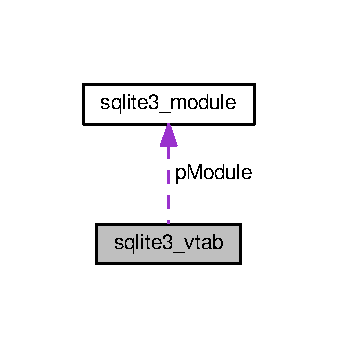
\includegraphics[width=162pt]{structsqlite3__vtab__coll__graph}
\end{center}
\end{figure}
\subsection*{Public Attributes}
\begin{DoxyCompactItemize}
\item 
const \hyperlink{structsqlite3__module}{sqlite3\+\_\+module} $\ast$ {\bfseries p\+Module}\hypertarget{structsqlite3__vtab_acf0d906e36b113669eaa883c5f8b5ba0}{}\label{structsqlite3__vtab_acf0d906e36b113669eaa883c5f8b5ba0}

\item 
int {\bfseries n\+Ref}\hypertarget{structsqlite3__vtab_ab3c80d385849bdd82363a0df7d6fcba8}{}\label{structsqlite3__vtab_ab3c80d385849bdd82363a0df7d6fcba8}

\item 
char $\ast$ {\bfseries z\+Err\+Msg}\hypertarget{structsqlite3__vtab_a47331586775d674ae951b07ebb902fca}{}\label{structsqlite3__vtab_a47331586775d674ae951b07ebb902fca}

\end{DoxyCompactItemize}


The documentation for this struct was generated from the following files\+:\begin{DoxyCompactItemize}
\item 
sqlite3.\+c\item 
sqlite3.\+h\end{DoxyCompactItemize}

\hypertarget{structsqlite3__vtab__cursor}{}\section{sqlite3\+\_\+vtab\+\_\+cursor Struct Reference}
\label{structsqlite3__vtab__cursor}\index{sqlite3\+\_\+vtab\+\_\+cursor@{sqlite3\+\_\+vtab\+\_\+cursor}}


Collaboration diagram for sqlite3\+\_\+vtab\+\_\+cursor\+:\nopagebreak
\begin{figure}[H]
\begin{center}
\leavevmode
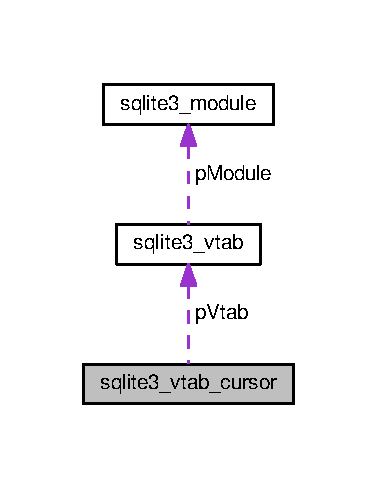
\includegraphics[width=181pt]{structsqlite3__vtab__cursor__coll__graph}
\end{center}
\end{figure}
\subsection*{Public Attributes}
\begin{DoxyCompactItemize}
\item 
\hyperlink{structsqlite3__vtab}{sqlite3\+\_\+vtab} $\ast$ {\bfseries p\+Vtab}\hypertarget{structsqlite3__vtab__cursor_a7bb57f3f9c7c618a9d6d33c6d9820bdc}{}\label{structsqlite3__vtab__cursor_a7bb57f3f9c7c618a9d6d33c6d9820bdc}

\end{DoxyCompactItemize}


The documentation for this struct was generated from the following files\+:\begin{DoxyCompactItemize}
\item 
sqlite3.\+c\item 
sqlite3.\+h\end{DoxyCompactItemize}

\hypertarget{structSqlite3Config}{}\section{Sqlite3\+Config Struct Reference}
\label{structSqlite3Config}\index{Sqlite3\+Config@{Sqlite3\+Config}}


Collaboration diagram for Sqlite3\+Config\+:
% FIG 0
\subsection*{Public Attributes}
\begin{DoxyCompactItemize}
\item 
int {\bfseries b\+Memstat}\hypertarget{structSqlite3Config_aae01de5f37a66422f2a7413e108e03fe}{}\label{structSqlite3Config_aae01de5f37a66422f2a7413e108e03fe}

\item 
int {\bfseries b\+Core\+Mutex}\hypertarget{structSqlite3Config_a202216a82e0823d0a4629c4884215a54}{}\label{structSqlite3Config_a202216a82e0823d0a4629c4884215a54}

\item 
int {\bfseries b\+Full\+Mutex}\hypertarget{structSqlite3Config_aab880bf54370cd0f6210afce0fb646ee}{}\label{structSqlite3Config_aab880bf54370cd0f6210afce0fb646ee}

\item 
int {\bfseries b\+Open\+Uri}\hypertarget{structSqlite3Config_af446c9f0657e5564b4dbba3421ffc8be}{}\label{structSqlite3Config_af446c9f0657e5564b4dbba3421ffc8be}

\item 
int {\bfseries b\+Use\+Cis}\hypertarget{structSqlite3Config_a3eb3eb5fe14358aba2a6e0083f29d807}{}\label{structSqlite3Config_a3eb3eb5fe14358aba2a6e0083f29d807}

\item 
int {\bfseries mx\+Strlen}\hypertarget{structSqlite3Config_a66f1f85ec9b7724f7fe0bebad61a634f}{}\label{structSqlite3Config_a66f1f85ec9b7724f7fe0bebad61a634f}

\item 
int {\bfseries never\+Corrupt}\hypertarget{structSqlite3Config_a6dc51cea630491a7c0694c1547894f1f}{}\label{structSqlite3Config_a6dc51cea630491a7c0694c1547894f1f}

\item 
int {\bfseries sz\+Lookaside}\hypertarget{structSqlite3Config_ad7504c4c1867db9837b40d7c22ba7582}{}\label{structSqlite3Config_ad7504c4c1867db9837b40d7c22ba7582}

\item 
int {\bfseries n\+Lookaside}\hypertarget{structSqlite3Config_a2519388eb9688eb3dbdc9b279ee73e0a}{}\label{structSqlite3Config_a2519388eb9688eb3dbdc9b279ee73e0a}

\item 
int {\bfseries n\+Stmt\+Spill}\hypertarget{structSqlite3Config_ac4976841f2245a238d41f2e1c6e05f91}{}\label{structSqlite3Config_ac4976841f2245a238d41f2e1c6e05f91}

\item 
\hyperlink{structsqlite3__mem__methods}{sqlite3\+\_\+mem\+\_\+methods} {\bfseries m}\hypertarget{structSqlite3Config_a922ec99508e346db8e4fbaec58aa1ff9}{}\label{structSqlite3Config_a922ec99508e346db8e4fbaec58aa1ff9}

\item 
\hyperlink{structsqlite3__mutex__methods}{sqlite3\+\_\+mutex\+\_\+methods} {\bfseries mutex}\hypertarget{structSqlite3Config_afa8189b51142fd800d1dee1987187f61}{}\label{structSqlite3Config_afa8189b51142fd800d1dee1987187f61}

\item 
\hyperlink{structsqlite3__pcache__methods2}{sqlite3\+\_\+pcache\+\_\+methods2} {\bfseries pcache2}\hypertarget{structSqlite3Config_ab1504fcfc7d18b64e26554a644ed9f6d}{}\label{structSqlite3Config_ab1504fcfc7d18b64e26554a644ed9f6d}

\item 
void $\ast$ {\bfseries p\+Heap}\hypertarget{structSqlite3Config_a52f66f1870b47adde44507d6bd523113}{}\label{structSqlite3Config_a52f66f1870b47adde44507d6bd523113}

\item 
int {\bfseries n\+Heap}\hypertarget{structSqlite3Config_a06d6d22e0fca1b713f9c7a110a89abba}{}\label{structSqlite3Config_a06d6d22e0fca1b713f9c7a110a89abba}

\item 
int {\bfseries mn\+Req}\hypertarget{structSqlite3Config_a2abbe78d2443b7408a01f59299da1174}{}\label{structSqlite3Config_a2abbe78d2443b7408a01f59299da1174}

\item 
int {\bfseries mx\+Req}\hypertarget{structSqlite3Config_a060f9ef5a2bda888a8253229384ab4a9}{}\label{structSqlite3Config_a060f9ef5a2bda888a8253229384ab4a9}

\item 
sqlite3\+\_\+int64 {\bfseries sz\+Mmap}\hypertarget{structSqlite3Config_ab5fb29ac41756c38a16bf3555adca853}{}\label{structSqlite3Config_ab5fb29ac41756c38a16bf3555adca853}

\item 
sqlite3\+\_\+int64 {\bfseries mx\+Mmap}\hypertarget{structSqlite3Config_a1e6bd364962243bc7c5de6867e4c8af2}{}\label{structSqlite3Config_a1e6bd364962243bc7c5de6867e4c8af2}

\item 
void $\ast$ {\bfseries p\+Scratch}\hypertarget{structSqlite3Config_aafbeaaeee4df0b98598c19a8af6cefed}{}\label{structSqlite3Config_aafbeaaeee4df0b98598c19a8af6cefed}

\item 
int {\bfseries sz\+Scratch}\hypertarget{structSqlite3Config_aed5cee0c084b3298b4f15debdab90272}{}\label{structSqlite3Config_aed5cee0c084b3298b4f15debdab90272}

\item 
int {\bfseries n\+Scratch}\hypertarget{structSqlite3Config_a63b88fc0b4f1dd3dfd11edc7ac0f657b}{}\label{structSqlite3Config_a63b88fc0b4f1dd3dfd11edc7ac0f657b}

\item 
void $\ast$ {\bfseries p\+Page}\hypertarget{structSqlite3Config_a059fe8443905388d65d741ba655438f9}{}\label{structSqlite3Config_a059fe8443905388d65d741ba655438f9}

\item 
int {\bfseries sz\+Page}\hypertarget{structSqlite3Config_aab2aff0daff6b09c1d77299c81892a28}{}\label{structSqlite3Config_aab2aff0daff6b09c1d77299c81892a28}

\item 
int {\bfseries n\+Page}\hypertarget{structSqlite3Config_a46af661bdb7a466b046a04b032868a36}{}\label{structSqlite3Config_a46af661bdb7a466b046a04b032868a36}

\item 
int {\bfseries mx\+Parser\+Stack}\hypertarget{structSqlite3Config_a5622c6caef3cd04007517a3a0c5e7ffe}{}\label{structSqlite3Config_a5622c6caef3cd04007517a3a0c5e7ffe}

\item 
int {\bfseries shared\+Cache\+Enabled}\hypertarget{structSqlite3Config_ad9837f5e2f338d708234afdb8878184f}{}\label{structSqlite3Config_ad9837f5e2f338d708234afdb8878184f}

\item 
u32 {\bfseries sz\+Pma}\hypertarget{structSqlite3Config_a189f09eced1df52e9d0d9ce95dde5f46}{}\label{structSqlite3Config_a189f09eced1df52e9d0d9ce95dde5f46}

\item 
int {\bfseries is\+Init}\hypertarget{structSqlite3Config_a11f18afbc3476ee16d97e75ad770670e}{}\label{structSqlite3Config_a11f18afbc3476ee16d97e75ad770670e}

\item 
int {\bfseries in\+Progress}\hypertarget{structSqlite3Config_a3cc1f0564475ead1840892e8ac6989ed}{}\label{structSqlite3Config_a3cc1f0564475ead1840892e8ac6989ed}

\item 
int {\bfseries is\+Mutex\+Init}\hypertarget{structSqlite3Config_af576d567cc36956e0c4c3a7487b53edf}{}\label{structSqlite3Config_af576d567cc36956e0c4c3a7487b53edf}

\item 
int {\bfseries is\+Malloc\+Init}\hypertarget{structSqlite3Config_ab0ec050075ee245df0a54623b0073bfc}{}\label{structSqlite3Config_ab0ec050075ee245df0a54623b0073bfc}

\item 
int {\bfseries is\+P\+Cache\+Init}\hypertarget{structSqlite3Config_a945ec3af8fd8f2efaccec88e2597393b}{}\label{structSqlite3Config_a945ec3af8fd8f2efaccec88e2597393b}

\item 
int {\bfseries n\+Ref\+Init\+Mutex}\hypertarget{structSqlite3Config_a423f5c1b3f68d9c569661a542ebe7220}{}\label{structSqlite3Config_a423f5c1b3f68d9c569661a542ebe7220}

\item 
\hyperlink{structsqlite3__mutex}{sqlite3\+\_\+mutex} $\ast$ {\bfseries p\+Init\+Mutex}\hypertarget{structSqlite3Config_af8ffb8388972c384840dd36beca35e7e}{}\label{structSqlite3Config_af8ffb8388972c384840dd36beca35e7e}

\item 
void($\ast$ {\bfseries x\+Log} )(void $\ast$, int, const char $\ast$)\hypertarget{structSqlite3Config_a3d9750f6c4fc73fdce5f83357184faae}{}\label{structSqlite3Config_a3d9750f6c4fc73fdce5f83357184faae}

\item 
void $\ast$ {\bfseries p\+Log\+Arg}\hypertarget{structSqlite3Config_a501ab4552bc7c54bb413aced5889dcdc}{}\label{structSqlite3Config_a501ab4552bc7c54bb413aced5889dcdc}

\item 
int($\ast$ {\bfseries x\+Test\+Callback} )(int)\hypertarget{structSqlite3Config_a6d21468c424041f10eb0c251220088f6}{}\label{structSqlite3Config_a6d21468c424041f10eb0c251220088f6}

\item 
int {\bfseries b\+Localtime\+Fault}\hypertarget{structSqlite3Config_a7bdc3109ecd839317f722b5da5339fab}{}\label{structSqlite3Config_a7bdc3109ecd839317f722b5da5339fab}

\item 
int {\bfseries i\+Once\+Reset\+Threshold}\hypertarget{structSqlite3Config_aed7a7e3bd6862ff2ca1444e16ad3948f}{}\label{structSqlite3Config_aed7a7e3bd6862ff2ca1444e16ad3948f}

\end{DoxyCompactItemize}


The documentation for this struct was generated from the following file\+:\begin{DoxyCompactItemize}
\item 
sqlite3.\+c\end{DoxyCompactItemize}

\hypertarget{structsqlite3_1_1sqlite3InitInfo}{}\section{sqlite3\+:\+:sqlite3\+Init\+Info Struct Reference}
\label{structsqlite3_1_1sqlite3InitInfo}\index{sqlite3\+::sqlite3\+Init\+Info@{sqlite3\+::sqlite3\+Init\+Info}}
\subsection*{Public Attributes}
\begin{DoxyCompactItemize}
\item 
int {\bfseries new\+Tnum}\hypertarget{structsqlite3_1_1sqlite3InitInfo_a65250c8c5f215989e64294ede6c1c268}{}\label{structsqlite3_1_1sqlite3InitInfo_a65250c8c5f215989e64294ede6c1c268}

\item 
u8 {\bfseries i\+Db}\hypertarget{structsqlite3_1_1sqlite3InitInfo_af72389cb54753544c0f578605e6604bb}{}\label{structsqlite3_1_1sqlite3InitInfo_af72389cb54753544c0f578605e6604bb}

\item 
u8 {\bfseries busy}\hypertarget{structsqlite3_1_1sqlite3InitInfo_a6ac01842e0ae68023cb60fea93bd8688}{}\label{structsqlite3_1_1sqlite3InitInfo_a6ac01842e0ae68023cb60fea93bd8688}

\item 
u8 {\bfseries orphan\+Trigger}\hypertarget{structsqlite3_1_1sqlite3InitInfo_ac292839cc81d109206133a80949c45a6}{}\label{structsqlite3_1_1sqlite3InitInfo_ac292839cc81d109206133a80949c45a6}

\item 
u8 {\bfseries imposter\+Table}\hypertarget{structsqlite3_1_1sqlite3InitInfo_a97d9d576e85a1752092122374a179139}{}\label{structsqlite3_1_1sqlite3InitInfo_a97d9d576e85a1752092122374a179139}

\end{DoxyCompactItemize}


The documentation for this struct was generated from the following file\+:\begin{DoxyCompactItemize}
\item 
sqlite3.\+c\end{DoxyCompactItemize}

\hypertarget{structSQLiteThread}{}\section{S\+Q\+Lite\+Thread Struct Reference}
\label{structSQLiteThread}\index{S\+Q\+Lite\+Thread@{S\+Q\+Lite\+Thread}}
\subsection*{Public Attributes}
\begin{DoxyCompactItemize}
\item 
pthread\+\_\+t {\bfseries tid}\hypertarget{structSQLiteThread_a344b7b30ad7f54c6cbfb4d2378982610}{}\label{structSQLiteThread_a344b7b30ad7f54c6cbfb4d2378982610}

\item 
int {\bfseries done}\hypertarget{structSQLiteThread_af13ecbf8ad23f24a5074277cdcf0383b}{}\label{structSQLiteThread_af13ecbf8ad23f24a5074277cdcf0383b}

\item 
void $\ast$ {\bfseries p\+Out}\hypertarget{structSQLiteThread_aca6d94405a6e7eefb230cd08bf1ce71b}{}\label{structSQLiteThread_aca6d94405a6e7eefb230cd08bf1ce71b}

\item 
void $\ast$($\ast$ {\bfseries x\+Task} )(void $\ast$)\hypertarget{structSQLiteThread_aadc8f1c225e769d42d981ae2e701d018}{}\label{structSQLiteThread_aadc8f1c225e769d42d981ae2e701d018}

\item 
void $\ast$ {\bfseries p\+In}\hypertarget{structSQLiteThread_ad14ce51f32c66b80c515ec2338f6ccd2}{}\label{structSQLiteThread_ad14ce51f32c66b80c515ec2338f6ccd2}

\end{DoxyCompactItemize}


The documentation for this struct was generated from the following file\+:\begin{DoxyCompactItemize}
\item 
sqlite3.\+c\end{DoxyCompactItemize}

\hypertarget{structSrcCount}{}\section{Src\+Count Struct Reference}
\label{structSrcCount}\index{Src\+Count@{Src\+Count}}


Collaboration diagram for Src\+Count\+:
% FIG 0
\subsection*{Public Attributes}
\begin{DoxyCompactItemize}
\item 
\hyperlink{structSrcList}{Src\+List} $\ast$ {\bfseries p\+Src}\hypertarget{structSrcCount_a7087f00bcaed39cc5032462d7262f4ff}{}\label{structSrcCount_a7087f00bcaed39cc5032462d7262f4ff}

\item 
int {\bfseries n\+This}\hypertarget{structSrcCount_a1aaa40ff75460ebc7778ea63aca14d4d}{}\label{structSrcCount_a1aaa40ff75460ebc7778ea63aca14d4d}

\item 
int {\bfseries n\+Other}\hypertarget{structSrcCount_a5666f8571b2877fdadfe95364ffb5b80}{}\label{structSrcCount_a5666f8571b2877fdadfe95364ffb5b80}

\end{DoxyCompactItemize}


The documentation for this struct was generated from the following file\+:\begin{DoxyCompactItemize}
\item 
sqlite3.\+c\end{DoxyCompactItemize}

\hypertarget{structSrcList}{}\section{Src\+List Struct Reference}
\label{structSrcList}\index{Src\+List@{Src\+List}}


Collaboration diagram for Src\+List\+:\nopagebreak
\begin{figure}[H]
\begin{center}
\leavevmode
\includegraphics[width=350pt]{structSrcList__coll__graph}
\end{center}
\end{figure}
\subsection*{Classes}
\begin{DoxyCompactItemize}
\item 
struct \hyperlink{structSrcList_1_1SrcList__item}{Src\+List\+\_\+item}
\end{DoxyCompactItemize}
\subsection*{Public Attributes}
\begin{DoxyCompactItemize}
\item 
int {\bfseries n\+Src}\hypertarget{structSrcList_a8ecf9cced910877d93210ace66365ec8}{}\label{structSrcList_a8ecf9cced910877d93210ace66365ec8}

\item 
u32 {\bfseries n\+Alloc}\hypertarget{structSrcList_ab9c572bef9144ab245f7f46bc5b82a61}{}\label{structSrcList_ab9c572bef9144ab245f7f46bc5b82a61}

\item 
struct \hyperlink{structSrcList_1_1SrcList__item}{Src\+List\+::\+Src\+List\+\_\+item} {\bfseries a} \mbox{[}1\mbox{]}\hypertarget{structSrcList_acd181938f7144b40022b28072247aa3d}{}\label{structSrcList_acd181938f7144b40022b28072247aa3d}

\end{DoxyCompactItemize}


The documentation for this struct was generated from the following file\+:\begin{DoxyCompactItemize}
\item 
sqlite3.\+c\end{DoxyCompactItemize}

\hypertarget{structSrcList_1_1SrcList__item}{}\section{Src\+List\+:\+:Src\+List\+\_\+item Struct Reference}
\label{structSrcList_1_1SrcList__item}\index{Src\+List\+::\+Src\+List\+\_\+item@{Src\+List\+::\+Src\+List\+\_\+item}}


Collaboration diagram for Src\+List\+:\+:Src\+List\+\_\+item\+:\nopagebreak
\begin{figure}[H]
\begin{center}
\leavevmode
\includegraphics[width=350pt]{structSrcList_1_1SrcList__item__coll__graph}
\end{center}
\end{figure}
\subsection*{Public Attributes}
\begin{DoxyCompactItemize}
\item 
\hyperlink{structSchema}{Schema} $\ast$ {\bfseries p\+Schema}\hypertarget{structSrcList_1_1SrcList__item_a021ffb4d9282b6ce171bd57c4da97bf3}{}\label{structSrcList_1_1SrcList__item_a021ffb4d9282b6ce171bd57c4da97bf3}

\item 
char $\ast$ {\bfseries z\+Database}\hypertarget{structSrcList_1_1SrcList__item_a2f7bf0921794dc46d74d2546fc10f7de}{}\label{structSrcList_1_1SrcList__item_a2f7bf0921794dc46d74d2546fc10f7de}

\item 
char $\ast$ {\bfseries z\+Name}\hypertarget{structSrcList_1_1SrcList__item_afee5c5a84594fed8100be3cdb3e3ff1c}{}\label{structSrcList_1_1SrcList__item_afee5c5a84594fed8100be3cdb3e3ff1c}

\item 
char $\ast$ {\bfseries z\+Alias}\hypertarget{structSrcList_1_1SrcList__item_a461ef8d80828ed8dd4409b9244ae2919}{}\label{structSrcList_1_1SrcList__item_a461ef8d80828ed8dd4409b9244ae2919}

\item 
\hyperlink{structTable}{Table} $\ast$ {\bfseries p\+Tab}\hypertarget{structSrcList_1_1SrcList__item_a8779b2d10d0e25af78ad90e57f9cd4f6}{}\label{structSrcList_1_1SrcList__item_a8779b2d10d0e25af78ad90e57f9cd4f6}

\item 
\hyperlink{structSelect}{Select} $\ast$ {\bfseries p\+Select}\hypertarget{structSrcList_1_1SrcList__item_ab44822fca7618c4f41f4f770ad41425b}{}\label{structSrcList_1_1SrcList__item_ab44822fca7618c4f41f4f770ad41425b}

\item 
int {\bfseries addr\+Fill\+Sub}\hypertarget{structSrcList_1_1SrcList__item_a1fb4f55d13641e11f07c3e535fd7cf1d}{}\label{structSrcList_1_1SrcList__item_a1fb4f55d13641e11f07c3e535fd7cf1d}

\item 
int {\bfseries reg\+Return}\hypertarget{structSrcList_1_1SrcList__item_a67344976677cbbdea271fcdf7be620cc}{}\label{structSrcList_1_1SrcList__item_a67344976677cbbdea271fcdf7be620cc}

\item 
int {\bfseries reg\+Result}\hypertarget{structSrcList_1_1SrcList__item_af4886ed7e335081909c2bfdd5d04c165}{}\label{structSrcList_1_1SrcList__item_af4886ed7e335081909c2bfdd5d04c165}

\item 
\begin{tabbing}
xx\=xx\=xx\=xx\=xx\=xx\=xx\=xx\=xx\=\kill
struct \{\\
\>u8 {\bfseries jointype}\\
\>unsigned {\bfseries notIndexed}:1\\
\>unsigned {\bfseries isIndexedBy}:1\\
\>unsigned {\bfseries isTabFunc}:1\\
\>unsigned {\bfseries isCorrelated}:1\\
\>unsigned {\bfseries viaCoroutine}:1\\
\>unsigned {\bfseries isRecursive}:1\\
\} {\bfseries fg}\hypertarget{structSrcList_1_1SrcList__item_a2defa6cd914167188e8e8ee48d173922}{}\label{structSrcList_1_1SrcList__item_a2defa6cd914167188e8e8ee48d173922}
\\

\end{tabbing}\item 
u8 {\bfseries i\+Select\+Id}\hypertarget{structSrcList_1_1SrcList__item_a099cfe9b7559b42c49dda02e57188738}{}\label{structSrcList_1_1SrcList__item_a099cfe9b7559b42c49dda02e57188738}

\item 
int {\bfseries i\+Cursor}\hypertarget{structSrcList_1_1SrcList__item_af2e8aae90bd7a00b814db5a2d31f6607}{}\label{structSrcList_1_1SrcList__item_af2e8aae90bd7a00b814db5a2d31f6607}

\item 
\hyperlink{structExpr}{Expr} $\ast$ {\bfseries p\+On}\hypertarget{structSrcList_1_1SrcList__item_a525f683af2ffa8f094d941a5a4972720}{}\label{structSrcList_1_1SrcList__item_a525f683af2ffa8f094d941a5a4972720}

\item 
\hyperlink{structIdList}{Id\+List} $\ast$ {\bfseries p\+Using}\hypertarget{structSrcList_1_1SrcList__item_a38ecf205dcaebad098b73c56e48ba944}{}\label{structSrcList_1_1SrcList__item_a38ecf205dcaebad098b73c56e48ba944}

\item 
Bitmask {\bfseries col\+Used}\hypertarget{structSrcList_1_1SrcList__item_a4fd7e7e26995048b58006d020e8c48d6}{}\label{structSrcList_1_1SrcList__item_a4fd7e7e26995048b58006d020e8c48d6}

\item 
\begin{tabbing}
xx\=xx\=xx\=xx\=xx\=xx\=xx\=xx\=xx\=\kill
union \{\\
\>char $\ast$ {\bfseries zIndexedBy}\\
\>\hyperlink{structExprList}{ExprList} $\ast$ {\bfseries pFuncArg}\\
\} {\bfseries u1}\hypertarget{structSrcList_1_1SrcList__item_a97bae7bc42769542d1ad49452a5016c9}{}\label{structSrcList_1_1SrcList__item_a97bae7bc42769542d1ad49452a5016c9}
\\

\end{tabbing}\item 
\hyperlink{structIndex}{Index} $\ast$ {\bfseries p\+I\+B\+Index}\hypertarget{structSrcList_1_1SrcList__item_a33f82c4d70c773856d55a5ebe9b1cc8c}{}\label{structSrcList_1_1SrcList__item_a33f82c4d70c773856d55a5ebe9b1cc8c}

\end{DoxyCompactItemize}


The documentation for this struct was generated from the following file\+:\begin{DoxyCompactItemize}
\item 
sqlite3.\+c\end{DoxyCompactItemize}

\hypertarget{structStat4Accum}{}\section{Stat4\+Accum Struct Reference}
\label{structStat4Accum}\index{Stat4\+Accum@{Stat4\+Accum}}


Collaboration diagram for Stat4\+Accum\+:\nopagebreak
\begin{figure}[H]
\begin{center}
\leavevmode
\includegraphics[width=350pt]{structStat4Accum__coll__graph}
\end{center}
\end{figure}
\subsection*{Public Attributes}
\begin{DoxyCompactItemize}
\item 
t\+Rowcnt {\bfseries n\+Row}\hypertarget{structStat4Accum_a7f06c1f2e4790e21b25aa68e5340f0b3}{}\label{structStat4Accum_a7f06c1f2e4790e21b25aa68e5340f0b3}

\item 
t\+Rowcnt {\bfseries n\+P\+Sample}\hypertarget{structStat4Accum_ac86c036108462008795ebfb7994ff674}{}\label{structStat4Accum_ac86c036108462008795ebfb7994ff674}

\item 
int {\bfseries n\+Col}\hypertarget{structStat4Accum_a4b5d9944be8bd28e2dcaaa10d23702db}{}\label{structStat4Accum_a4b5d9944be8bd28e2dcaaa10d23702db}

\item 
int {\bfseries n\+Key\+Col}\hypertarget{structStat4Accum_a018b3aa526f4d376e55042e290c935c4}{}\label{structStat4Accum_a018b3aa526f4d376e55042e290c935c4}

\item 
int {\bfseries mx\+Sample}\hypertarget{structStat4Accum_a2133206dd5209b1b0fce485bc6d48043}{}\label{structStat4Accum_a2133206dd5209b1b0fce485bc6d48043}

\item 
\hyperlink{structStat4Sample}{Stat4\+Sample} {\bfseries current}\hypertarget{structStat4Accum_a9e65f562b6944448edde933a6d29fdf2}{}\label{structStat4Accum_a9e65f562b6944448edde933a6d29fdf2}

\item 
u32 {\bfseries i\+Prn}\hypertarget{structStat4Accum_a13746aceec404f569af80ee44c9315ac}{}\label{structStat4Accum_a13746aceec404f569af80ee44c9315ac}

\item 
\hyperlink{structStat4Sample}{Stat4\+Sample} $\ast$ {\bfseries a\+Best}\hypertarget{structStat4Accum_a634729ee0061b7243e770b6281d9a7a4}{}\label{structStat4Accum_a634729ee0061b7243e770b6281d9a7a4}

\item 
int {\bfseries i\+Min}\hypertarget{structStat4Accum_a9935fae376aa4010a0d205e7a3283d36}{}\label{structStat4Accum_a9935fae376aa4010a0d205e7a3283d36}

\item 
int {\bfseries n\+Sample}\hypertarget{structStat4Accum_ae96fc8b759131bd3d968086a009a9170}{}\label{structStat4Accum_ae96fc8b759131bd3d968086a009a9170}

\item 
int {\bfseries i\+Get}\hypertarget{structStat4Accum_aee70ce1c45daa00581265d27337bce5e}{}\label{structStat4Accum_aee70ce1c45daa00581265d27337bce5e}

\item 
\hyperlink{structStat4Sample}{Stat4\+Sample} $\ast$ {\bfseries a}\hypertarget{structStat4Accum_a921a2a1d92fe8113626bde517d004278}{}\label{structStat4Accum_a921a2a1d92fe8113626bde517d004278}

\item 
\hyperlink{structsqlite3}{sqlite3} $\ast$ {\bfseries db}\hypertarget{structStat4Accum_af0ae3ddd7a24a925ebe090db6f06a12b}{}\label{structStat4Accum_af0ae3ddd7a24a925ebe090db6f06a12b}

\end{DoxyCompactItemize}


The documentation for this struct was generated from the following file\+:\begin{DoxyCompactItemize}
\item 
sqlite3.\+c\end{DoxyCompactItemize}

\hypertarget{structStat4Sample}{}\section{Stat4\+Sample Struct Reference}
\label{structStat4Sample}\index{Stat4\+Sample@{Stat4\+Sample}}
\subsection*{Public Attributes}
\begin{DoxyCompactItemize}
\item 
t\+Rowcnt $\ast$ {\bfseries an\+Eq}\hypertarget{structStat4Sample_a8dd17556ec12614fbf4b88ab0bc82749}{}\label{structStat4Sample_a8dd17556ec12614fbf4b88ab0bc82749}

\item 
t\+Rowcnt $\ast$ {\bfseries an\+D\+Lt}\hypertarget{structStat4Sample_a25519389bab21052bf80af8500388a37}{}\label{structStat4Sample_a25519389bab21052bf80af8500388a37}

\end{DoxyCompactItemize}


The documentation for this struct was generated from the following file\+:\begin{DoxyCompactItemize}
\item 
sqlite3.\+c\end{DoxyCompactItemize}

\hypertarget{structStrAccum}{}\section{Str\+Accum Struct Reference}
\label{structStrAccum}\index{Str\+Accum@{Str\+Accum}}


Collaboration diagram for Str\+Accum\+:\nopagebreak
\begin{figure}[H]
\begin{center}
\leavevmode
\includegraphics[width=350pt]{structStrAccum__coll__graph}
\end{center}
\end{figure}
\subsection*{Public Attributes}
\begin{DoxyCompactItemize}
\item 
\hyperlink{structsqlite3}{sqlite3} $\ast$ {\bfseries db}\hypertarget{structStrAccum_ade44091c9a91671c9457b9e4a98a9a5d}{}\label{structStrAccum_ade44091c9a91671c9457b9e4a98a9a5d}

\item 
char $\ast$ {\bfseries z\+Base}\hypertarget{structStrAccum_a5797e2f288573ee98a4025f0f96fe50d}{}\label{structStrAccum_a5797e2f288573ee98a4025f0f96fe50d}

\item 
char $\ast$ {\bfseries z\+Text}\hypertarget{structStrAccum_ac45a51cb7b85da2ae9865eac21d416dc}{}\label{structStrAccum_ac45a51cb7b85da2ae9865eac21d416dc}

\item 
u32 {\bfseries n\+Char}\hypertarget{structStrAccum_a9ae2f859cd15934c7fd1ed2243782607}{}\label{structStrAccum_a9ae2f859cd15934c7fd1ed2243782607}

\item 
u32 {\bfseries n\+Alloc}\hypertarget{structStrAccum_a48d37540058f35811bd37c5ee56e0c93}{}\label{structStrAccum_a48d37540058f35811bd37c5ee56e0c93}

\item 
u32 {\bfseries mx\+Alloc}\hypertarget{structStrAccum_a113c466027421582120b873ba342529c}{}\label{structStrAccum_a113c466027421582120b873ba342529c}

\item 
u8 {\bfseries acc\+Error}\hypertarget{structStrAccum_a0ff9aa2eca1d5dc78692721e2a56dc1e}{}\label{structStrAccum_a0ff9aa2eca1d5dc78692721e2a56dc1e}

\item 
u8 {\bfseries printf\+Flags}\hypertarget{structStrAccum_a95038abba91f6ec1a74c9dfc4fec0df9}{}\label{structStrAccum_a95038abba91f6ec1a74c9dfc4fec0df9}

\end{DoxyCompactItemize}


The documentation for this struct was generated from the following file\+:\begin{DoxyCompactItemize}
\item 
sqlite3.\+c\end{DoxyCompactItemize}

\hypertarget{structSubProgram}{}\section{Sub\+Program Struct Reference}
\label{structSubProgram}\index{Sub\+Program@{Sub\+Program}}


Collaboration diagram for Sub\+Program\+:
% FIG 0
\subsection*{Public Attributes}
\begin{DoxyCompactItemize}
\item 
\hyperlink{structVdbeOp}{Vdbe\+Op} $\ast$ {\bfseries a\+Op}\hypertarget{structSubProgram_aa9bb1992fed633d182076a35d6448c7d}{}\label{structSubProgram_aa9bb1992fed633d182076a35d6448c7d}

\item 
int {\bfseries n\+Op}\hypertarget{structSubProgram_a6fe204a75ab8254c453be77f024b6d69}{}\label{structSubProgram_a6fe204a75ab8254c453be77f024b6d69}

\item 
int {\bfseries n\+Mem}\hypertarget{structSubProgram_a9bece42fdeb81085809d7c2f8aa05616}{}\label{structSubProgram_a9bece42fdeb81085809d7c2f8aa05616}

\item 
int {\bfseries n\+Csr}\hypertarget{structSubProgram_a83b18aa5cc63aecdbf996c16af1e48bb}{}\label{structSubProgram_a83b18aa5cc63aecdbf996c16af1e48bb}

\item 
void $\ast$ {\bfseries token}\hypertarget{structSubProgram_aaea3b67899b092476b107d22a4e2022d}{}\label{structSubProgram_aaea3b67899b092476b107d22a4e2022d}

\item 
\hyperlink{structSubProgram}{Sub\+Program} $\ast$ {\bfseries p\+Next}\hypertarget{structSubProgram_a7da35488ac58a64fa30b88da56aac8b3}{}\label{structSubProgram_a7da35488ac58a64fa30b88da56aac8b3}

\end{DoxyCompactItemize}


The documentation for this struct was generated from the following file\+:\begin{DoxyCompactItemize}
\item 
sqlite3.\+c\end{DoxyCompactItemize}

\hypertarget{structSumCtx}{}\section{Sum\+Ctx Struct Reference}
\label{structSumCtx}\index{Sum\+Ctx@{Sum\+Ctx}}
\subsection*{Public Attributes}
\begin{DoxyCompactItemize}
\item 
double {\bfseries r\+Sum}\hypertarget{structSumCtx_a1774080b9bcada2f4e867eaf40763f41}{}\label{structSumCtx_a1774080b9bcada2f4e867eaf40763f41}

\item 
i64 {\bfseries i\+Sum}\hypertarget{structSumCtx_ace6196fb30ebc0687997a723d55683db}{}\label{structSumCtx_ace6196fb30ebc0687997a723d55683db}

\item 
i64 {\bfseries cnt}\hypertarget{structSumCtx_ada00261fe604a7cc6719fdcd8bb5914c}{}\label{structSumCtx_ada00261fe604a7cc6719fdcd8bb5914c}

\item 
u8 {\bfseries overflow}\hypertarget{structSumCtx_a3b14a5da00584aff08314d5e9ddbe9ea}{}\label{structSumCtx_a3b14a5da00584aff08314d5e9ddbe9ea}

\item 
u8 {\bfseries approx}\hypertarget{structSumCtx_a035a2a22271fee066d9a92d12fe3b9a5}{}\label{structSumCtx_a035a2a22271fee066d9a92d12fe3b9a5}

\end{DoxyCompactItemize}


The documentation for this struct was generated from the following file\+:\begin{DoxyCompactItemize}
\item 
sqlite3.\+c\end{DoxyCompactItemize}

\hypertarget{structTable}{}\section{Table Struct Reference}
\label{structTable}\index{Table@{Table}}


Collaboration diagram for Table\+:\nopagebreak
\begin{figure}[H]
\begin{center}
\leavevmode
\includegraphics[width=350pt]{structTable__coll__graph}
\end{center}
\end{figure}
\subsection*{Public Attributes}
\begin{DoxyCompactItemize}
\item 
char $\ast$ {\bfseries z\+Name}\hypertarget{structTable_a20ca62607d6da596b1016b76cf677809}{}\label{structTable_a20ca62607d6da596b1016b76cf677809}

\item 
\hyperlink{structColumn}{Column} $\ast$ {\bfseries a\+Col}\hypertarget{structTable_a87ec3b706ecf9545bd9ed582a12ce3e7}{}\label{structTable_a87ec3b706ecf9545bd9ed582a12ce3e7}

\item 
\hyperlink{structIndex}{Index} $\ast$ {\bfseries p\+Index}\hypertarget{structTable_a5dffd0c9e8f0265d6a47b32bd0e6d59f}{}\label{structTable_a5dffd0c9e8f0265d6a47b32bd0e6d59f}

\item 
\hyperlink{structSelect}{Select} $\ast$ {\bfseries p\+Select}\hypertarget{structTable_a39d620182fe2174fc97d04094421fa60}{}\label{structTable_a39d620182fe2174fc97d04094421fa60}

\item 
\hyperlink{structFKey}{F\+Key} $\ast$ {\bfseries p\+F\+Key}\hypertarget{structTable_a37ccce5ee6d530001d49c82788c6616d}{}\label{structTable_a37ccce5ee6d530001d49c82788c6616d}

\item 
char $\ast$ {\bfseries z\+Col\+Aff}\hypertarget{structTable_ac95c0c7b04f2c8367beb98d386d4228f}{}\label{structTable_ac95c0c7b04f2c8367beb98d386d4228f}

\item 
\hyperlink{structExprList}{Expr\+List} $\ast$ {\bfseries p\+Check}\hypertarget{structTable_a4513ad39c4adad36fdf5dd3c6cb70a12}{}\label{structTable_a4513ad39c4adad36fdf5dd3c6cb70a12}

\item 
int {\bfseries tnum}\hypertarget{structTable_aebe1abbfb2fd4b5e5dff8e74a4f3c890}{}\label{structTable_aebe1abbfb2fd4b5e5dff8e74a4f3c890}

\item 
i16 {\bfseries i\+P\+Key}\hypertarget{structTable_af5e592498393a990cb1344555fa86409}{}\label{structTable_af5e592498393a990cb1344555fa86409}

\item 
i16 {\bfseries n\+Col}\hypertarget{structTable_a1a8346811ba23fdfd90c5b54076bbefb}{}\label{structTable_a1a8346811ba23fdfd90c5b54076bbefb}

\item 
u16 {\bfseries n\+Ref}\hypertarget{structTable_a5c3d59f52186917d412d42e008dd302c}{}\label{structTable_a5c3d59f52186917d412d42e008dd302c}

\item 
Log\+Est {\bfseries n\+Row\+Log\+Est}\hypertarget{structTable_ae3835f1c227f6f14ec412d04fae854aa}{}\label{structTable_ae3835f1c227f6f14ec412d04fae854aa}

\item 
Log\+Est {\bfseries sz\+Tab\+Row}\hypertarget{structTable_a141c547347c585b17f9ca2664967ab75}{}\label{structTable_a141c547347c585b17f9ca2664967ab75}

\item 
u8 {\bfseries tab\+Flags}\hypertarget{structTable_ab0aeb112ae7e1b81e2a18bc493f7992c}{}\label{structTable_ab0aeb112ae7e1b81e2a18bc493f7992c}

\item 
u8 {\bfseries key\+Conf}\hypertarget{structTable_add1b22425db781d976d25b4465a2965a}{}\label{structTable_add1b22425db781d976d25b4465a2965a}

\item 
int {\bfseries add\+Col\+Offset}\hypertarget{structTable_ab6f1ad10bce5c20faca55cd0a9c3f1ff}{}\label{structTable_ab6f1ad10bce5c20faca55cd0a9c3f1ff}

\item 
int {\bfseries n\+Module\+Arg}\hypertarget{structTable_a74a2c5547ea876ebe77dbea0d99361bf}{}\label{structTable_a74a2c5547ea876ebe77dbea0d99361bf}

\item 
char $\ast$$\ast$ {\bfseries az\+Module\+Arg}\hypertarget{structTable_af3af6596efa41894bcd3c3c9f9b6781f}{}\label{structTable_af3af6596efa41894bcd3c3c9f9b6781f}

\item 
\hyperlink{structVTable}{V\+Table} $\ast$ {\bfseries p\+V\+Table}\hypertarget{structTable_a7b9903cfbfefe7b8bf872c4f50cb2e95}{}\label{structTable_a7b9903cfbfefe7b8bf872c4f50cb2e95}

\item 
\hyperlink{structTrigger}{Trigger} $\ast$ {\bfseries p\+Trigger}\hypertarget{structTable_aca61c40bb0164f2c6fc3406c28988660}{}\label{structTable_aca61c40bb0164f2c6fc3406c28988660}

\item 
\hyperlink{structSchema}{Schema} $\ast$ {\bfseries p\+Schema}\hypertarget{structTable_a1d6ce038a061722cebaeba0f3ffceacf}{}\label{structTable_a1d6ce038a061722cebaeba0f3ffceacf}

\item 
\hyperlink{structTable}{Table} $\ast$ {\bfseries p\+Next\+Zombie}\hypertarget{structTable_ae365eb0d8f6d3cb39f3908323cba45e4}{}\label{structTable_ae365eb0d8f6d3cb39f3908323cba45e4}

\end{DoxyCompactItemize}


The documentation for this struct was generated from the following file\+:\begin{DoxyCompactItemize}
\item 
sqlite3.\+c\end{DoxyCompactItemize}

\hypertarget{structTableLock}{}\section{Table\+Lock Struct Reference}
\label{structTableLock}\index{Table\+Lock@{Table\+Lock}}
\subsection*{Public Attributes}
\begin{DoxyCompactItemize}
\item 
int {\bfseries i\+Db}\hypertarget{structTableLock_ad5cc726ef29ffcca39ec0b72942513f6}{}\label{structTableLock_ad5cc726ef29ffcca39ec0b72942513f6}

\item 
int {\bfseries i\+Tab}\hypertarget{structTableLock_ab25b5d9ba21ed96ed68ce8064ff84e24}{}\label{structTableLock_ab25b5d9ba21ed96ed68ce8064ff84e24}

\item 
u8 {\bfseries is\+Write\+Lock}\hypertarget{structTableLock_a171121af9886ee08044d4b82b991ceeb}{}\label{structTableLock_a171121af9886ee08044d4b82b991ceeb}

\item 
const char $\ast$ {\bfseries z\+Name}\hypertarget{structTableLock_ad1ce077fbd2600dd6d23ec08706dd227}{}\label{structTableLock_ad1ce077fbd2600dd6d23ec08706dd227}

\end{DoxyCompactItemize}


The documentation for this struct was generated from the following file\+:\begin{DoxyCompactItemize}
\item 
sqlite3.\+c\end{DoxyCompactItemize}

\hypertarget{structTabResult}{}\section{Tab\+Result Struct Reference}
\label{structTabResult}\index{Tab\+Result@{Tab\+Result}}
\subsection*{Public Attributes}
\begin{DoxyCompactItemize}
\item 
char $\ast$$\ast$ {\bfseries az\+Result}\hypertarget{structTabResult_a7446a22a7b39c17e447c65ba200490a6}{}\label{structTabResult_a7446a22a7b39c17e447c65ba200490a6}

\item 
char $\ast$ {\bfseries z\+Err\+Msg}\hypertarget{structTabResult_a6e7104bb622be05f16b6470dbb68a6c7}{}\label{structTabResult_a6e7104bb622be05f16b6470dbb68a6c7}

\item 
u32 {\bfseries n\+Alloc}\hypertarget{structTabResult_a9d07a6698e6b0293cf26fa3d39d222ea}{}\label{structTabResult_a9d07a6698e6b0293cf26fa3d39d222ea}

\item 
u32 {\bfseries n\+Row}\hypertarget{structTabResult_a0c2a87855e7665334ec4f39cc4e2fe8b}{}\label{structTabResult_a0c2a87855e7665334ec4f39cc4e2fe8b}

\item 
u32 {\bfseries n\+Column}\hypertarget{structTabResult_a34f54427ffc26de952a3df8fd50a3cca}{}\label{structTabResult_a34f54427ffc26de952a3df8fd50a3cca}

\item 
u32 {\bfseries n\+Data}\hypertarget{structTabResult_a15ec3f09bc4ccc6945c2e76bf32cf457}{}\label{structTabResult_a15ec3f09bc4ccc6945c2e76bf32cf457}

\item 
int {\bfseries rc}\hypertarget{structTabResult_a44bb015ce660ed3f987e324919d73f4d}{}\label{structTabResult_a44bb015ce660ed3f987e324919d73f4d}

\end{DoxyCompactItemize}


The documentation for this struct was generated from the following file\+:\begin{DoxyCompactItemize}
\item 
sqlite3.\+c\end{DoxyCompactItemize}

\hypertarget{structToken}{}\section{Token Struct Reference}
\label{structToken}\index{Token@{Token}}
\subsection*{Public Attributes}
\begin{DoxyCompactItemize}
\item 
const char $\ast$ {\bfseries z}\hypertarget{structToken_a57b502141e3018e4a02773424acb4ffd}{}\label{structToken_a57b502141e3018e4a02773424acb4ffd}

\item 
unsigned int {\bfseries n}\hypertarget{structToken_ad8442439e00ab9713a9b91a53e44c2aa}{}\label{structToken_ad8442439e00ab9713a9b91a53e44c2aa}

\end{DoxyCompactItemize}


The documentation for this struct was generated from the following file\+:\begin{DoxyCompactItemize}
\item 
sqlite3.\+c\end{DoxyCompactItemize}

\hypertarget{structTrigEvent}{}\section{Trig\+Event Struct Reference}
\label{structTrigEvent}\index{Trig\+Event@{Trig\+Event}}


Collaboration diagram for Trig\+Event\+:
% FIG 0
\subsection*{Public Attributes}
\begin{DoxyCompactItemize}
\item 
int {\bfseries a}\hypertarget{structTrigEvent_a19ac5a5e59e08350f72ec49cf8fccbb6}{}\label{structTrigEvent_a19ac5a5e59e08350f72ec49cf8fccbb6}

\item 
\hyperlink{structIdList}{Id\+List} $\ast$ {\bfseries b}\hypertarget{structTrigEvent_a86ef160cde95382e98b7934614e7f79f}{}\label{structTrigEvent_a86ef160cde95382e98b7934614e7f79f}

\end{DoxyCompactItemize}


The documentation for this struct was generated from the following file\+:\begin{DoxyCompactItemize}
\item 
sqlite3.\+c\end{DoxyCompactItemize}

\hypertarget{structTrigger}{}\section{Trigger Struct Reference}
\label{structTrigger}\index{Trigger@{Trigger}}


Collaboration diagram for Trigger\+:
% FIG 0
\subsection*{Public Attributes}
\begin{DoxyCompactItemize}
\item 
char $\ast$ {\bfseries z\+Name}\hypertarget{structTrigger_a9aecea5dadd7ae93b7f585c4b914791c}{}\label{structTrigger_a9aecea5dadd7ae93b7f585c4b914791c}

\item 
char $\ast$ {\bfseries table}\hypertarget{structTrigger_ab9d5500f7fc43382e867733a2968ecae}{}\label{structTrigger_ab9d5500f7fc43382e867733a2968ecae}

\item 
u8 {\bfseries op}\hypertarget{structTrigger_a855d6b6a302d8d80e1d30ddd70fd403e}{}\label{structTrigger_a855d6b6a302d8d80e1d30ddd70fd403e}

\item 
u8 {\bfseries tr\+\_\+tm}\hypertarget{structTrigger_af0d10da140b068bfd76aaeb6607fa6cf}{}\label{structTrigger_af0d10da140b068bfd76aaeb6607fa6cf}

\item 
\hyperlink{structExpr}{Expr} $\ast$ {\bfseries p\+When}\hypertarget{structTrigger_a1b6cdd46e8b98562920d1acee86281ed}{}\label{structTrigger_a1b6cdd46e8b98562920d1acee86281ed}

\item 
\hyperlink{structIdList}{Id\+List} $\ast$ {\bfseries p\+Columns}\hypertarget{structTrigger_a8505fbdf63ca9eadf4b2585e99faa4e4}{}\label{structTrigger_a8505fbdf63ca9eadf4b2585e99faa4e4}

\item 
\hyperlink{structSchema}{Schema} $\ast$ {\bfseries p\+Schema}\hypertarget{structTrigger_a83edbfa91ce6520a6ebc1a21acc2cd5e}{}\label{structTrigger_a83edbfa91ce6520a6ebc1a21acc2cd5e}

\item 
\hyperlink{structSchema}{Schema} $\ast$ {\bfseries p\+Tab\+Schema}\hypertarget{structTrigger_a8e4a9b3f4bcc5c645e1777b3bb94a6d8}{}\label{structTrigger_a8e4a9b3f4bcc5c645e1777b3bb94a6d8}

\item 
\hyperlink{structTriggerStep}{Trigger\+Step} $\ast$ {\bfseries step\+\_\+list}\hypertarget{structTrigger_a4206faaae6cdf1a2b22a2c9f15c88642}{}\label{structTrigger_a4206faaae6cdf1a2b22a2c9f15c88642}

\item 
\hyperlink{structTrigger}{Trigger} $\ast$ {\bfseries p\+Next}\hypertarget{structTrigger_ac28107e1c45789e0146fe45867b8dfdb}{}\label{structTrigger_ac28107e1c45789e0146fe45867b8dfdb}

\end{DoxyCompactItemize}


The documentation for this struct was generated from the following file\+:\begin{DoxyCompactItemize}
\item 
sqlite3.\+c\end{DoxyCompactItemize}

\hypertarget{structTriggerPrg}{}\section{Trigger\+Prg Struct Reference}
\label{structTriggerPrg}\index{Trigger\+Prg@{Trigger\+Prg}}


Collaboration diagram for Trigger\+Prg\+:\nopagebreak
\begin{figure}[H]
\begin{center}
\leavevmode
\includegraphics[width=350pt]{structTriggerPrg__coll__graph}
\end{center}
\end{figure}
\subsection*{Public Attributes}
\begin{DoxyCompactItemize}
\item 
\hyperlink{structTrigger}{Trigger} $\ast$ {\bfseries p\+Trigger}\hypertarget{structTriggerPrg_af70e5a74c954bc7a1eb8ee1162c40368}{}\label{structTriggerPrg_af70e5a74c954bc7a1eb8ee1162c40368}

\item 
\hyperlink{structTriggerPrg}{Trigger\+Prg} $\ast$ {\bfseries p\+Next}\hypertarget{structTriggerPrg_a551b8a29a8c4ff785afab1596e5d8710}{}\label{structTriggerPrg_a551b8a29a8c4ff785afab1596e5d8710}

\item 
\hyperlink{structSubProgram}{Sub\+Program} $\ast$ {\bfseries p\+Program}\hypertarget{structTriggerPrg_aa770aee270c7c5df85578dc4a6686134}{}\label{structTriggerPrg_aa770aee270c7c5df85578dc4a6686134}

\item 
int {\bfseries orconf}\hypertarget{structTriggerPrg_aa475acda58c472b3491f6aa17020bf68}{}\label{structTriggerPrg_aa475acda58c472b3491f6aa17020bf68}

\item 
u32 {\bfseries a\+Colmask} \mbox{[}2\mbox{]}\hypertarget{structTriggerPrg_aeac0a4cd1f1d287981ae33c4d171b614}{}\label{structTriggerPrg_aeac0a4cd1f1d287981ae33c4d171b614}

\end{DoxyCompactItemize}


The documentation for this struct was generated from the following file\+:\begin{DoxyCompactItemize}
\item 
sqlite3.\+c\end{DoxyCompactItemize}

\hypertarget{structTriggerStep}{}\section{Trigger\+Step Struct Reference}
\label{structTriggerStep}\index{Trigger\+Step@{Trigger\+Step}}


Collaboration diagram for Trigger\+Step\+:\nopagebreak
\begin{figure}[H]
\begin{center}
\leavevmode
\includegraphics[width=350pt]{structTriggerStep__coll__graph}
\end{center}
\end{figure}
\subsection*{Public Attributes}
\begin{DoxyCompactItemize}
\item 
u8 {\bfseries op}\hypertarget{structTriggerStep_a20269855c80d869d498fcb93401832fd}{}\label{structTriggerStep_a20269855c80d869d498fcb93401832fd}

\item 
u8 {\bfseries orconf}\hypertarget{structTriggerStep_a4ed8b2571fde96e84f637184453e73e3}{}\label{structTriggerStep_a4ed8b2571fde96e84f637184453e73e3}

\item 
\hyperlink{structTrigger}{Trigger} $\ast$ {\bfseries p\+Trig}\hypertarget{structTriggerStep_a70671e85796776db06c732ab6ae4ae0d}{}\label{structTriggerStep_a70671e85796776db06c732ab6ae4ae0d}

\item 
\hyperlink{structSelect}{Select} $\ast$ {\bfseries p\+Select}\hypertarget{structTriggerStep_a90bf3353653cedf364a7fb2eb89a19c4}{}\label{structTriggerStep_a90bf3353653cedf364a7fb2eb89a19c4}

\item 
char $\ast$ {\bfseries z\+Target}\hypertarget{structTriggerStep_a5e48fd22b4e42ca72ae6e505861483df}{}\label{structTriggerStep_a5e48fd22b4e42ca72ae6e505861483df}

\item 
\hyperlink{structExpr}{Expr} $\ast$ {\bfseries p\+Where}\hypertarget{structTriggerStep_ad4c293b04dfda535f3aad5b9e02726c7}{}\label{structTriggerStep_ad4c293b04dfda535f3aad5b9e02726c7}

\item 
\hyperlink{structExprList}{Expr\+List} $\ast$ {\bfseries p\+Expr\+List}\hypertarget{structTriggerStep_a607602af65ecf6c7e6cac4ea8532ac1d}{}\label{structTriggerStep_a607602af65ecf6c7e6cac4ea8532ac1d}

\item 
\hyperlink{structIdList}{Id\+List} $\ast$ {\bfseries p\+Id\+List}\hypertarget{structTriggerStep_a6b91bf578544104f8bd4bd5b958ddd8c}{}\label{structTriggerStep_a6b91bf578544104f8bd4bd5b958ddd8c}

\item 
\hyperlink{structTriggerStep}{Trigger\+Step} $\ast$ {\bfseries p\+Next}\hypertarget{structTriggerStep_a0757a0d22dbe2f7f57706014dd35759b}{}\label{structTriggerStep_a0757a0d22dbe2f7f57706014dd35759b}

\item 
\hyperlink{structTriggerStep}{Trigger\+Step} $\ast$ {\bfseries p\+Last}\hypertarget{structTriggerStep_a0aae9ea7f436881c0e9e614476a69584}{}\label{structTriggerStep_a0aae9ea7f436881c0e9e614476a69584}

\end{DoxyCompactItemize}


The documentation for this struct was generated from the following file\+:\begin{DoxyCompactItemize}
\item 
sqlite3.\+c\end{DoxyCompactItemize}

\hypertarget{classTruck}{}\section{Truck Class Reference}
\label{classTruck}\index{Truck@{Truck}}


\hyperlink{classTruck}{Truck} Class.  




{\ttfamily \#include $<$Truck.\+h$>$}

\subsection*{Public Member Functions}
\begin{DoxyCompactItemize}
\item 
\hyperlink{classTruck_a139a26bbf66738685b66a5747bffdc2c}{Truck} (const double)
\begin{DoxyCompactList}\small\item\em \hyperlink{classTruck}{Truck} constructor. \end{DoxyCompactList}\item 
int \hyperlink{classTruck_ac6d9654486fdae70caaecad8ff6ec561}{get\+Truck\+ID} () const 
\begin{DoxyCompactList}\small\item\em Getter for \hyperlink{classTruck}{Truck} ID Number. \end{DoxyCompactList}\item 
double \hyperlink{classTruck_ab4e29138dc4a6c430f0b365180cac978}{get\+Weight} () const 
\begin{DoxyCompactList}\small\item\em Getter for truck\textquotesingle{}s weight limit. \end{DoxyCompactList}\item 
vector$<$ \hyperlink{classPackage}{Package} $\ast$ $>$ \hyperlink{classTruck_a6448f8b9d6cfaaaf5e2bc21b9e103685}{get\+Packages} () const 
\begin{DoxyCompactList}\small\item\em Getter for package vector. \end{DoxyCompactList}\item 
vector$<$ string $\ast$ $>$ \hyperlink{classTruck_a80092b55170e601b68dd2cd184933079}{get\+Directions} () const 
\begin{DoxyCompactList}\small\item\em Getter for directions vector. \end{DoxyCompactList}\item 
void \hyperlink{classTruck_ad08c796603bfc23896abe4d71ac7a9ac}{set\+Directions} (vector$<$ string $\ast$ $>$)
\begin{DoxyCompactList}\small\item\em Setter for directions vector. \end{DoxyCompactList}\item 
vector$<$ pair$<$ int, int $>$ $>$ \hyperlink{classTruck_a511bd8447763c46b25a131b4decb04c5}{get\+Stops} () const 
\begin{DoxyCompactList}\small\item\em getter for vector of stops as cartesian coordinates \end{DoxyCompactList}\item 
void \hyperlink{classTruck_a7d021abea77aac57190922a78279edcd}{set\+Stops} (const vector$<$ pair$<$ int, int $>$ $>$ \&)
\begin{DoxyCompactList}\small\item\em setter for vector of stops as cartesian coordinates \end{DoxyCompactList}\item 
void \hyperlink{classTruck_ad4c15f435c3e7f7851b7ffa018ac198e}{add\+Package} (\hyperlink{classPackage}{Package} $\ast$)
\begin{DoxyCompactList}\small\item\em Adds a package to the truck. \end{DoxyCompactList}\item 
void \hyperlink{classTruck_a51d480fbf34068dcd6512f8fd43aadf9}{deliver\+Package} (\hyperlink{classPackage}{Package} $\ast$pack)
\begin{DoxyCompactList}\small\item\em Delivers a package. \end{DoxyCompactList}\item 
string \hyperlink{classTruck_afc282688d1ad6a3ad79a0060c4e7d63c}{to\+String} () const 
\begin{DoxyCompactList}\small\item\em Returns a string representation of the truck and its contents. \end{DoxyCompactList}\end{DoxyCompactItemize}
\subsection*{Static Public Attributes}
\begin{DoxyCompactItemize}
\item 
static int \hyperlink{classTruck_a7435e6c1e97d263f36897f8ade5d4c41}{truck\+Count} = 0
\begin{DoxyCompactList}\small\item\em A count of the total number of trucks on the road. \end{DoxyCompactList}\end{DoxyCompactItemize}
\subsection*{Private Attributes}
\begin{DoxyCompactItemize}
\item 
const int \hyperlink{classTruck_a7552538334822cb0526b3b714fcc09fc}{truck\+ID}\hypertarget{classTruck_a7552538334822cb0526b3b714fcc09fc}{}\label{classTruck_a7552538334822cb0526b3b714fcc09fc}

\begin{DoxyCompactList}\small\item\em This truck\textquotesingle{}s identification number. \end{DoxyCompactList}\item 
double \hyperlink{classTruck_a51f90c7e56b08f4ad92436233326f746}{weight}\hypertarget{classTruck_a51f90c7e56b08f4ad92436233326f746}{}\label{classTruck_a51f90c7e56b08f4ad92436233326f746}

\begin{DoxyCompactList}\small\item\em This truck\textquotesingle{}s weight limit. \end{DoxyCompactList}\item 
double \hyperlink{classTruck_af1817d5b13eecfd5f3a6037eb76de31f}{current\+Weight} = 0\hypertarget{classTruck_af1817d5b13eecfd5f3a6037eb76de31f}{}\label{classTruck_af1817d5b13eecfd5f3a6037eb76de31f}

\begin{DoxyCompactList}\small\item\em The current weight of the truck\textquotesingle{}s load of packages. \end{DoxyCompactList}\item 
vector$<$ \hyperlink{classPackage}{Package} $\ast$ $>$ {\bfseries packages}\hypertarget{classTruck_a56932c0950c2a2a129e557f003980ffc}{}\label{classTruck_a56932c0950c2a2a129e557f003980ffc}

\item 
vector$<$ pair$<$ int, int $>$ $>$ \hyperlink{classTruck_a72e3a307480578a189c8446f16556be8}{stops}\hypertarget{classTruck_a72e3a307480578a189c8446f16556be8}{}\label{classTruck_a72e3a307480578a189c8446f16556be8}

\begin{DoxyCompactList}\small\item\em Vector of addresses as cartesian coordinates. \end{DoxyCompactList}\item 
vector$<$ string $\ast$ $>$ \hyperlink{classTruck_a62316796e456b748a80c870e41e058f4}{directions}\hypertarget{classTruck_a62316796e456b748a80c870e41e058f4}{}\label{classTruck_a62316796e456b748a80c870e41e058f4}

\begin{DoxyCompactList}\small\item\em Vector of strings storing the directions for this truck. \end{DoxyCompactList}\end{DoxyCompactItemize}


\subsection{Detailed Description}
\hyperlink{classTruck}{Truck} Class. 

This \hyperlink{classTruck}{Truck} class defines a truck. It is responsible for holding a list of all packages in its delivery queue and a list of instructions for delivering those packages. 

\subsection{Constructor \& Destructor Documentation}
\index{Truck@{Truck}!Truck@{Truck}}
\index{Truck@{Truck}!Truck@{Truck}}
\subsubsection[{\texorpdfstring{Truck(const double)}{Truck(const double)}}]{\setlength{\rightskip}{0pt plus 5cm}Truck\+::\+Truck (
\begin{DoxyParamCaption}
\item[{const double}]{w}
\end{DoxyParamCaption}
)}\hypertarget{classTruck_a139a26bbf66738685b66a5747bffdc2c}{}\label{classTruck_a139a26bbf66738685b66a5747bffdc2c}


\hyperlink{classTruck}{Truck} constructor. 

Constructor.


\begin{DoxyParams}{Parameters}
{\em weight} & Weight limit\\
\hline
{\em w} & Weight limit for this truck \\
\hline
\end{DoxyParams}


\subsection{Member Function Documentation}
\index{Truck@{Truck}!add\+Package@{add\+Package}}
\index{add\+Package@{add\+Package}!Truck@{Truck}}
\subsubsection[{\texorpdfstring{add\+Package(\+Package $\ast$)}{addPackage(Package *)}}]{\setlength{\rightskip}{0pt plus 5cm}void Truck\+::add\+Package (
\begin{DoxyParamCaption}
\item[{{\bf Package} $\ast$}]{pack}
\end{DoxyParamCaption}
)}\hypertarget{classTruck_ad4c15f435c3e7f7851b7ffa018ac198e}{}\label{classTruck_ad4c15f435c3e7f7851b7ffa018ac198e}


Adds a package to the truck. 

Add a package to the truck.

Adds a package to the truck and adds its weight to the current load 
\begin{DoxyParams}{Parameters}
{\em pack} & A package object\\
\hline
\end{DoxyParams}
Adds a package to the truck. If this would go over the weight limit of the truck, then it throws an error. It also adds the weight of the package to the truck if the package fits. 
\begin{DoxyParams}{Parameters}
{\em $\ast$pack} & Pointer to package \\
\hline
\end{DoxyParams}
\index{Truck@{Truck}!deliver\+Package@{deliver\+Package}}
\index{deliver\+Package@{deliver\+Package}!Truck@{Truck}}
\subsubsection[{\texorpdfstring{deliver\+Package(\+Package $\ast$pack)}{deliverPackage(Package *pack)}}]{\setlength{\rightskip}{0pt plus 5cm}void Truck\+::deliver\+Package (
\begin{DoxyParamCaption}
\item[{{\bf Package} $\ast$}]{pack}
\end{DoxyParamCaption}
)}\hypertarget{classTruck_a51d480fbf34068dcd6512f8fd43aadf9}{}\label{classTruck_a51d480fbf34068dcd6512f8fd43aadf9}


Delivers a package. 

Delivers package.

Removes a package from the truck, subtracts its weight, and sets the package\textquotesingle{}s delivered flag.

sets delivered flag to true if this package is in the vector \index{Truck@{Truck}!get\+Directions@{get\+Directions}}
\index{get\+Directions@{get\+Directions}!Truck@{Truck}}
\subsubsection[{\texorpdfstring{get\+Directions() const }{getDirections() const }}]{\setlength{\rightskip}{0pt plus 5cm}vector$<$ string $\ast$ $>$ Truck\+::get\+Directions (
\begin{DoxyParamCaption}
{}
\end{DoxyParamCaption}
) const}\hypertarget{classTruck_a80092b55170e601b68dd2cd184933079}{}\label{classTruck_a80092b55170e601b68dd2cd184933079}


Getter for directions vector. 

Get directions assigned to this truck.

\begin{DoxyReturn}{Returns}
the vector containing the truck\textquotesingle{}s current list of directions

vector$<$string$\ast$$>$ 
\end{DoxyReturn}
\index{Truck@{Truck}!get\+Packages@{get\+Packages}}
\index{get\+Packages@{get\+Packages}!Truck@{Truck}}
\subsubsection[{\texorpdfstring{get\+Packages() const }{getPackages() const }}]{\setlength{\rightskip}{0pt plus 5cm}vector$<$ {\bf Package} $\ast$ $>$ Truck\+::get\+Packages (
\begin{DoxyParamCaption}
{}
\end{DoxyParamCaption}
) const}\hypertarget{classTruck_a6448f8b9d6cfaaaf5e2bc21b9e103685}{}\label{classTruck_a6448f8b9d6cfaaaf5e2bc21b9e103685}


Getter for package vector. 

Gets truck\textquotesingle{}s currently loaded packages.

return vector$<$\+Package$\ast$$>$ \index{Truck@{Truck}!get\+Stops@{get\+Stops}}
\index{get\+Stops@{get\+Stops}!Truck@{Truck}}
\subsubsection[{\texorpdfstring{get\+Stops() const }{getStops() const }}]{\setlength{\rightskip}{0pt plus 5cm}vector$<$ pair$<$ int, int $>$ $>$ Truck\+::get\+Stops (
\begin{DoxyParamCaption}
{}
\end{DoxyParamCaption}
) const}\hypertarget{classTruck_a511bd8447763c46b25a131b4decb04c5}{}\label{classTruck_a511bd8447763c46b25a131b4decb04c5}


getter for vector of stops as cartesian coordinates 

Getter for list of stops as cartesian coordinates.

\begin{DoxyReturn}{Returns}
vector$<$int,int$>$ $>$ a vector of pair$<$int, int$>$ $>$ 
\end{DoxyReturn}
\index{Truck@{Truck}!get\+Truck\+ID@{get\+Truck\+ID}}
\index{get\+Truck\+ID@{get\+Truck\+ID}!Truck@{Truck}}
\subsubsection[{\texorpdfstring{get\+Truck\+I\+D() const }{getTruckID() const }}]{\setlength{\rightskip}{0pt plus 5cm}int Truck\+::get\+Truck\+ID (
\begin{DoxyParamCaption}
{}
\end{DoxyParamCaption}
) const}\hypertarget{classTruck_ac6d9654486fdae70caaecad8ff6ec561}{}\label{classTruck_ac6d9654486fdae70caaecad8ff6ec561}


Getter for \hyperlink{classTruck}{Truck} ID Number. 

Gets this truck\textquotesingle{}s ID number.

\begin{DoxyReturn}{Returns}
int \hyperlink{classTruck}{Truck} ID number
\end{DoxyReturn}
return int \index{Truck@{Truck}!get\+Weight@{get\+Weight}}
\index{get\+Weight@{get\+Weight}!Truck@{Truck}}
\subsubsection[{\texorpdfstring{get\+Weight() const }{getWeight() const }}]{\setlength{\rightskip}{0pt plus 5cm}double Truck\+::get\+Weight (
\begin{DoxyParamCaption}
{}
\end{DoxyParamCaption}
) const}\hypertarget{classTruck_ab4e29138dc4a6c430f0b365180cac978}{}\label{classTruck_ab4e29138dc4a6c430f0b365180cac978}


Getter for truck\textquotesingle{}s weight limit. 

Gets truck\textquotesingle{}s weight limit.

\begin{DoxyReturn}{Returns}
double \hyperlink{classTruck}{Truck}\textquotesingle{}s weight limit

double 
\end{DoxyReturn}
\index{Truck@{Truck}!set\+Directions@{set\+Directions}}
\index{set\+Directions@{set\+Directions}!Truck@{Truck}}
\subsubsection[{\texorpdfstring{set\+Directions(vector$<$ string $\ast$ $>$)}{setDirections(vector< string * >)}}]{\setlength{\rightskip}{0pt plus 5cm}void Truck\+::set\+Directions (
\begin{DoxyParamCaption}
\item[{vector$<$ string $\ast$ $>$}]{direct}
\end{DoxyParamCaption}
)}\hypertarget{classTruck_ad08c796603bfc23896abe4d71ac7a9ac}{}\label{classTruck_ad08c796603bfc23896abe4d71ac7a9ac}


Setter for directions vector. 


\begin{DoxyParams}{Parameters}
{\em directions} & a pointer to a vector contianing the truck\textquotesingle{}s assigned directions\\
\hline
{\em direct} & pointer to directions vector \\
\hline
\end{DoxyParams}
\index{Truck@{Truck}!set\+Stops@{set\+Stops}}
\index{set\+Stops@{set\+Stops}!Truck@{Truck}}
\subsubsection[{\texorpdfstring{set\+Stops(const vector$<$ pair$<$ int, int $>$ $>$ \&)}{setStops(const vector< pair< int, int > > &)}}]{\setlength{\rightskip}{0pt plus 5cm}void Truck\+::set\+Stops (
\begin{DoxyParamCaption}
\item[{const vector$<$ pair$<$ int, int $>$ $>$ \&}]{s}
\end{DoxyParamCaption}
)}\hypertarget{classTruck_a7d021abea77aac57190922a78279edcd}{}\label{classTruck_a7d021abea77aac57190922a78279edcd}


setter for vector of stops as cartesian coordinates 

Setter for list of stops as cartesian coordinates.


\begin{DoxyParams}{Parameters}
{\em s} & vector of stops as cartesian coordinates \\
\hline
\end{DoxyParams}
\index{Truck@{Truck}!to\+String@{to\+String}}
\index{to\+String@{to\+String}!Truck@{Truck}}
\subsubsection[{\texorpdfstring{to\+String() const }{toString() const }}]{\setlength{\rightskip}{0pt plus 5cm}string Truck\+::to\+String (
\begin{DoxyParamCaption}
{}
\end{DoxyParamCaption}
) const}\hypertarget{classTruck_afc282688d1ad6a3ad79a0060c4e7d63c}{}\label{classTruck_afc282688d1ad6a3ad79a0060c4e7d63c}


Returns a string representation of the truck and its contents. 

To string.

\begin{DoxyReturn}{Returns}
string A string representation of the truck and its contents 
\end{DoxyReturn}


\subsection{Member Data Documentation}
\index{Truck@{Truck}!truck\+Count@{truck\+Count}}
\index{truck\+Count@{truck\+Count}!Truck@{Truck}}
\subsubsection[{\texorpdfstring{truck\+Count}{truckCount}}]{\setlength{\rightskip}{0pt plus 5cm}int Truck\+::truck\+Count = 0\hspace{0.3cm}{\ttfamily [static]}}\hypertarget{classTruck_a7435e6c1e97d263f36897f8ade5d4c41}{}\label{classTruck_a7435e6c1e97d263f36897f8ade5d4c41}


A count of the total number of trucks on the road. 

Initialize truck count. 

The documentation for this class was generated from the following files\+:\begin{DoxyCompactItemize}
\item 
Truck.\+h\item 
Truck.\+cpp\end{DoxyCompactItemize}

\hypertarget{structunixFile}{}\section{unix\+File Struct Reference}
\label{structunixFile}\index{unix\+File@{unix\+File}}


Collaboration diagram for unix\+File\+:
% FIG 0
\subsection*{Public Attributes}
\begin{DoxyCompactItemize}
\item 
\hyperlink{structsqlite3__io__methods}{sqlite3\+\_\+io\+\_\+methods} const $\ast$ {\bfseries p\+Method}\hypertarget{structunixFile_a2a2b40e965f91aa9ee21135bfb0c17ec}{}\label{structunixFile_a2a2b40e965f91aa9ee21135bfb0c17ec}

\item 
\hyperlink{structsqlite3__vfs}{sqlite3\+\_\+vfs} $\ast$ {\bfseries p\+Vfs}\hypertarget{structunixFile_a048d696479bb2544ab2cec1ac9a75d67}{}\label{structunixFile_a048d696479bb2544ab2cec1ac9a75d67}

\item 
\hyperlink{structunixInodeInfo}{unix\+Inode\+Info} $\ast$ {\bfseries p\+Inode}\hypertarget{structunixFile_ac17292fe29bb6cc9eceed9db6d1209e8}{}\label{structunixFile_ac17292fe29bb6cc9eceed9db6d1209e8}

\item 
int {\bfseries h}\hypertarget{structunixFile_a1c58798d4ff3ac6232765c8b76bb7450}{}\label{structunixFile_a1c58798d4ff3ac6232765c8b76bb7450}

\item 
unsigned char {\bfseries e\+File\+Lock}\hypertarget{structunixFile_a001e59bdb9d3f396952c2c8e3229f7fc}{}\label{structunixFile_a001e59bdb9d3f396952c2c8e3229f7fc}

\item 
unsigned short int {\bfseries ctrl\+Flags}\hypertarget{structunixFile_a05d9d0af8aa4d9de6a250984cc12ae56}{}\label{structunixFile_a05d9d0af8aa4d9de6a250984cc12ae56}

\item 
int {\bfseries last\+Errno}\hypertarget{structunixFile_afde57c2e118fac8041918dac2ee6f7d1}{}\label{structunixFile_afde57c2e118fac8041918dac2ee6f7d1}

\item 
void $\ast$ {\bfseries locking\+Context}\hypertarget{structunixFile_afaeb4425a6de3e913db4b03e8a0d098a}{}\label{structunixFile_afaeb4425a6de3e913db4b03e8a0d098a}

\item 
\hyperlink{structUnixUnusedFd}{Unix\+Unused\+Fd} $\ast$ {\bfseries p\+Unused}\hypertarget{structunixFile_a3820ccead5805d2ea61ca1c752646852}{}\label{structunixFile_a3820ccead5805d2ea61ca1c752646852}

\item 
const char $\ast$ {\bfseries z\+Path}\hypertarget{structunixFile_afc5eff0948d553308cf90a79d4a06f17}{}\label{structunixFile_afc5eff0948d553308cf90a79d4a06f17}

\item 
\hyperlink{structunixShm}{unix\+Shm} $\ast$ {\bfseries p\+Shm}\hypertarget{structunixFile_a53c653bd73cdc6f518ecffe95062e91a}{}\label{structunixFile_a53c653bd73cdc6f518ecffe95062e91a}

\item 
int {\bfseries sz\+Chunk}\hypertarget{structunixFile_a5f6307d3446ce1b149df756c00c3bd2e}{}\label{structunixFile_a5f6307d3446ce1b149df756c00c3bd2e}

\end{DoxyCompactItemize}


The documentation for this struct was generated from the following file\+:\begin{DoxyCompactItemize}
\item 
sqlite3.\+c\end{DoxyCompactItemize}

\hypertarget{structunixFileId}{}\section{unix\+File\+Id Struct Reference}
\label{structunixFileId}\index{unix\+File\+Id@{unix\+File\+Id}}
\subsection*{Public Attributes}
\begin{DoxyCompactItemize}
\item 
dev\+\_\+t {\bfseries dev}\hypertarget{structunixFileId_acf703d95b9a1ae2f34affb7e9ae45e1b}{}\label{structunixFileId_acf703d95b9a1ae2f34affb7e9ae45e1b}

\item 
ino\+\_\+t {\bfseries ino}\hypertarget{structunixFileId_a2cc2d43e9d3f0a60810daa8fc353e692}{}\label{structunixFileId_a2cc2d43e9d3f0a60810daa8fc353e692}

\end{DoxyCompactItemize}


The documentation for this struct was generated from the following file\+:\begin{DoxyCompactItemize}
\item 
sqlite3.\+c\end{DoxyCompactItemize}

\hypertarget{structunixInodeInfo}{}\section{unix\+Inode\+Info Struct Reference}
\label{structunixInodeInfo}\index{unix\+Inode\+Info@{unix\+Inode\+Info}}


Collaboration diagram for unix\+Inode\+Info\+:
% FIG 0
\subsection*{Public Attributes}
\begin{DoxyCompactItemize}
\item 
struct \hyperlink{structunixFileId}{unix\+File\+Id} {\bfseries file\+Id}\hypertarget{structunixInodeInfo_ae692731d449f4462a921dda9a061faa6}{}\label{structunixInodeInfo_ae692731d449f4462a921dda9a061faa6}

\item 
int {\bfseries n\+Shared}\hypertarget{structunixInodeInfo_a0d7f8dd92964f53e59c8d741dbe00a61}{}\label{structunixInodeInfo_a0d7f8dd92964f53e59c8d741dbe00a61}

\item 
unsigned char {\bfseries e\+File\+Lock}\hypertarget{structunixInodeInfo_a010a765bb3feecb16b650f68fc3a3c1f}{}\label{structunixInodeInfo_a010a765bb3feecb16b650f68fc3a3c1f}

\item 
unsigned char {\bfseries b\+Process\+Lock}\hypertarget{structunixInodeInfo_ade689e4231dd80bb33c86da1e5ed1586}{}\label{structunixInodeInfo_ade689e4231dd80bb33c86da1e5ed1586}

\item 
int {\bfseries n\+Ref}\hypertarget{structunixInodeInfo_a65cbd1fd05ed00f03a252266b04a8221}{}\label{structunixInodeInfo_a65cbd1fd05ed00f03a252266b04a8221}

\item 
\hyperlink{structunixShmNode}{unix\+Shm\+Node} $\ast$ {\bfseries p\+Shm\+Node}\hypertarget{structunixInodeInfo_a302a8b82e27d5b3624ec122bc9c2ed61}{}\label{structunixInodeInfo_a302a8b82e27d5b3624ec122bc9c2ed61}

\item 
int {\bfseries n\+Lock}\hypertarget{structunixInodeInfo_a477f3357a32adbc1a9b05017e535444d}{}\label{structunixInodeInfo_a477f3357a32adbc1a9b05017e535444d}

\item 
\hyperlink{structUnixUnusedFd}{Unix\+Unused\+Fd} $\ast$ {\bfseries p\+Unused}\hypertarget{structunixInodeInfo_a0dda9ad35734fa161d1f0b13b671c1c6}{}\label{structunixInodeInfo_a0dda9ad35734fa161d1f0b13b671c1c6}

\item 
\hyperlink{structunixInodeInfo}{unix\+Inode\+Info} $\ast$ {\bfseries p\+Next}\hypertarget{structunixInodeInfo_a80181ba4ef71dd0d8e55e97baedc761e}{}\label{structunixInodeInfo_a80181ba4ef71dd0d8e55e97baedc761e}

\item 
\hyperlink{structunixInodeInfo}{unix\+Inode\+Info} $\ast$ {\bfseries p\+Prev}\hypertarget{structunixInodeInfo_a6575edce9898b48870c6f48047c01d01}{}\label{structunixInodeInfo_a6575edce9898b48870c6f48047c01d01}

\end{DoxyCompactItemize}


The documentation for this struct was generated from the following file\+:\begin{DoxyCompactItemize}
\item 
sqlite3.\+c\end{DoxyCompactItemize}

\hypertarget{structunixShm}{}\section{unix\+Shm Struct Reference}
\label{structunixShm}\index{unix\+Shm@{unix\+Shm}}


Collaboration diagram for unix\+Shm\+:\nopagebreak
\begin{figure}[H]
\begin{center}
\leavevmode
\includegraphics[width=350pt]{structunixShm__coll__graph}
\end{center}
\end{figure}
\subsection*{Public Attributes}
\begin{DoxyCompactItemize}
\item 
\hyperlink{structunixShmNode}{unix\+Shm\+Node} $\ast$ {\bfseries p\+Shm\+Node}\hypertarget{structunixShm_a8ab421232d29e3237262ef46775199ee}{}\label{structunixShm_a8ab421232d29e3237262ef46775199ee}

\item 
\hyperlink{structunixShm}{unix\+Shm} $\ast$ {\bfseries p\+Next}\hypertarget{structunixShm_a0d5229cf734581f51cdf16dd7d5ce93a}{}\label{structunixShm_a0d5229cf734581f51cdf16dd7d5ce93a}

\item 
u8 {\bfseries has\+Mutex}\hypertarget{structunixShm_a43903be262472299c5eee917ba7c523c}{}\label{structunixShm_a43903be262472299c5eee917ba7c523c}

\item 
u8 {\bfseries id}\hypertarget{structunixShm_a88a5e7161ff31f85740dbfc0ba7ad38a}{}\label{structunixShm_a88a5e7161ff31f85740dbfc0ba7ad38a}

\item 
u16 {\bfseries shared\+Mask}\hypertarget{structunixShm_a768aa62a6ea2bd91ab60a34d7654811b}{}\label{structunixShm_a768aa62a6ea2bd91ab60a34d7654811b}

\item 
u16 {\bfseries excl\+Mask}\hypertarget{structunixShm_ac6f786d95952e51cab941cbfb9243c8e}{}\label{structunixShm_ac6f786d95952e51cab941cbfb9243c8e}

\end{DoxyCompactItemize}


The documentation for this struct was generated from the following file\+:\begin{DoxyCompactItemize}
\item 
sqlite3.\+c\end{DoxyCompactItemize}

\hypertarget{structunixShmNode}{}\section{unix\+Shm\+Node Struct Reference}
\label{structunixShmNode}\index{unix\+Shm\+Node@{unix\+Shm\+Node}}


Collaboration diagram for unix\+Shm\+Node\+:
% FIG 0
\subsection*{Public Attributes}
\begin{DoxyCompactItemize}
\item 
\hyperlink{structunixInodeInfo}{unix\+Inode\+Info} $\ast$ {\bfseries p\+Inode}\hypertarget{structunixShmNode_ab6bc1cf84d65887a3395da6406843817}{}\label{structunixShmNode_ab6bc1cf84d65887a3395da6406843817}

\item 
\hyperlink{structsqlite3__mutex}{sqlite3\+\_\+mutex} $\ast$ {\bfseries mutex}\hypertarget{structunixShmNode_aa90850530f48fec6f2a872874f8ddf1f}{}\label{structunixShmNode_aa90850530f48fec6f2a872874f8ddf1f}

\item 
char $\ast$ {\bfseries z\+Filename}\hypertarget{structunixShmNode_a188c3bc5fcb4666ad0817ac093e7505d}{}\label{structunixShmNode_a188c3bc5fcb4666ad0817ac093e7505d}

\item 
int {\bfseries h}\hypertarget{structunixShmNode_a9cd93c8052eb47f257e2d752e8f1fdba}{}\label{structunixShmNode_a9cd93c8052eb47f257e2d752e8f1fdba}

\item 
int {\bfseries sz\+Region}\hypertarget{structunixShmNode_ae8126f9db70a758c2f340ec06869e02b}{}\label{structunixShmNode_ae8126f9db70a758c2f340ec06869e02b}

\item 
u16 {\bfseries n\+Region}\hypertarget{structunixShmNode_aaf1fceb640b3959424403885c0419a46}{}\label{structunixShmNode_aaf1fceb640b3959424403885c0419a46}

\item 
u8 {\bfseries is\+Readonly}\hypertarget{structunixShmNode_ad241b0a85f01110310cea91aa38fccb2}{}\label{structunixShmNode_ad241b0a85f01110310cea91aa38fccb2}

\item 
char $\ast$$\ast$ {\bfseries ap\+Region}\hypertarget{structunixShmNode_a8eff550f9b10a2de463e9874f84efc5e}{}\label{structunixShmNode_a8eff550f9b10a2de463e9874f84efc5e}

\item 
int {\bfseries n\+Ref}\hypertarget{structunixShmNode_a6d9f0c9dec3f6710cb09c90723a8284b}{}\label{structunixShmNode_a6d9f0c9dec3f6710cb09c90723a8284b}

\item 
\hyperlink{structunixShm}{unix\+Shm} $\ast$ {\bfseries p\+First}\hypertarget{structunixShmNode_a0ddd6c4625acf5994a60b0c368bc665e}{}\label{structunixShmNode_a0ddd6c4625acf5994a60b0c368bc665e}

\end{DoxyCompactItemize}


The documentation for this struct was generated from the following file\+:\begin{DoxyCompactItemize}
\item 
sqlite3.\+c\end{DoxyCompactItemize}

\hypertarget{structUnixUnusedFd}{}\section{Unix\+Unused\+Fd Struct Reference}
\label{structUnixUnusedFd}\index{Unix\+Unused\+Fd@{Unix\+Unused\+Fd}}


Collaboration diagram for Unix\+Unused\+Fd\+:
% FIG 0
\subsection*{Public Attributes}
\begin{DoxyCompactItemize}
\item 
int {\bfseries fd}\hypertarget{structUnixUnusedFd_a3f1a6127218af971aeb7b131c9c1600d}{}\label{structUnixUnusedFd_a3f1a6127218af971aeb7b131c9c1600d}

\item 
int {\bfseries flags}\hypertarget{structUnixUnusedFd_a744cd118bd91ec2019108e8205708684}{}\label{structUnixUnusedFd_a744cd118bd91ec2019108e8205708684}

\item 
\hyperlink{structUnixUnusedFd}{Unix\+Unused\+Fd} $\ast$ {\bfseries p\+Next}\hypertarget{structUnixUnusedFd_a6bbcba75beeabdd2df126638bc1d8bc0}{}\label{structUnixUnusedFd_a6bbcba75beeabdd2df126638bc1d8bc0}

\end{DoxyCompactItemize}


The documentation for this struct was generated from the following file\+:\begin{DoxyCompactItemize}
\item 
sqlite3.\+c\end{DoxyCompactItemize}

\hypertarget{structUnpackedRecord}{}\section{Unpacked\+Record Struct Reference}
\label{structUnpackedRecord}\index{Unpacked\+Record@{Unpacked\+Record}}


Collaboration diagram for Unpacked\+Record\+:
% FIG 0
\subsection*{Public Attributes}
\begin{DoxyCompactItemize}
\item 
\hyperlink{structKeyInfo}{Key\+Info} $\ast$ {\bfseries p\+Key\+Info}\hypertarget{structUnpackedRecord_aeb43e7a1e300857cab2cbe98eacd575b}{}\label{structUnpackedRecord_aeb43e7a1e300857cab2cbe98eacd575b}

\item 
\hyperlink{structMem}{Mem} $\ast$ {\bfseries a\+Mem}\hypertarget{structUnpackedRecord_a3299c322ceb8b758dacc59701021ae9f}{}\label{structUnpackedRecord_a3299c322ceb8b758dacc59701021ae9f}

\item 
u16 {\bfseries n\+Field}\hypertarget{structUnpackedRecord_a2c5062735cdbc5039679d255cc900668}{}\label{structUnpackedRecord_a2c5062735cdbc5039679d255cc900668}

\item 
i8 {\bfseries default\+\_\+rc}\hypertarget{structUnpackedRecord_a8f18c6e59de409bf543de0965652faa9}{}\label{structUnpackedRecord_a8f18c6e59de409bf543de0965652faa9}

\item 
u8 {\bfseries err\+Code}\hypertarget{structUnpackedRecord_a5c42d9878256f14c87f0e099b31da4bb}{}\label{structUnpackedRecord_a5c42d9878256f14c87f0e099b31da4bb}

\item 
i8 {\bfseries r1}\hypertarget{structUnpackedRecord_aff1dc6903bbc46b232d912bd25683b8a}{}\label{structUnpackedRecord_aff1dc6903bbc46b232d912bd25683b8a}

\item 
i8 {\bfseries r2}\hypertarget{structUnpackedRecord_a57a0cc8800e409d46c7c804bc68b5b2b}{}\label{structUnpackedRecord_a57a0cc8800e409d46c7c804bc68b5b2b}

\item 
u8 {\bfseries eq\+Seen}\hypertarget{structUnpackedRecord_a2efeb544b71d5e6c98b39ac845380e4e}{}\label{structUnpackedRecord_a2efeb544b71d5e6c98b39ac845380e4e}

\end{DoxyCompactItemize}


The documentation for this struct was generated from the following file\+:\begin{DoxyCompactItemize}
\item 
sqlite3.\+c\end{DoxyCompactItemize}

\hypertarget{structValueNewStat4Ctx}{}\section{Value\+New\+Stat4\+Ctx Struct Reference}
\label{structValueNewStat4Ctx}\index{Value\+New\+Stat4\+Ctx@{Value\+New\+Stat4\+Ctx}}


Collaboration diagram for Value\+New\+Stat4\+Ctx\+:\nopagebreak
\begin{figure}[H]
\begin{center}
\leavevmode
\includegraphics[width=350pt]{structValueNewStat4Ctx__coll__graph}
\end{center}
\end{figure}
\subsection*{Public Attributes}
\begin{DoxyCompactItemize}
\item 
\hyperlink{structParse}{Parse} $\ast$ {\bfseries p\+Parse}\hypertarget{structValueNewStat4Ctx_aa1d5c751a45f4e608dbd883179dd2f18}{}\label{structValueNewStat4Ctx_aa1d5c751a45f4e608dbd883179dd2f18}

\item 
\hyperlink{structIndex}{Index} $\ast$ {\bfseries p\+Idx}\hypertarget{structValueNewStat4Ctx_a31a0ab3baf8fab451df095591408acad}{}\label{structValueNewStat4Ctx_a31a0ab3baf8fab451df095591408acad}

\item 
\hyperlink{structUnpackedRecord}{Unpacked\+Record} $\ast$$\ast$ {\bfseries pp\+Rec}\hypertarget{structValueNewStat4Ctx_a64e1490828ea95f9edc650a776a121d9}{}\label{structValueNewStat4Ctx_a64e1490828ea95f9edc650a776a121d9}

\item 
int {\bfseries i\+Val}\hypertarget{structValueNewStat4Ctx_a54d56872d3653e59a00a91ea1c6b7664}{}\label{structValueNewStat4Ctx_a54d56872d3653e59a00a91ea1c6b7664}

\end{DoxyCompactItemize}


The documentation for this struct was generated from the following file\+:\begin{DoxyCompactItemize}
\item 
sqlite3.\+c\end{DoxyCompactItemize}

\hypertarget{structVdbe}{}\section{Vdbe Struct Reference}
\label{structVdbe}\index{Vdbe@{Vdbe}}


Collaboration diagram for Vdbe\+:
% FIG 0
\subsection*{Public Attributes}
\begin{DoxyCompactItemize}
\item 
\hyperlink{structsqlite3}{sqlite3} $\ast$ {\bfseries db}\hypertarget{structVdbe_a495366101a593999f4d2ed905e839029}{}\label{structVdbe_a495366101a593999f4d2ed905e839029}

\item 
\hyperlink{structVdbe}{Vdbe} $\ast$ {\bfseries p\+Prev}\hypertarget{structVdbe_a2afc3b6cd2f5b38d991148b809b3c53f}{}\label{structVdbe_a2afc3b6cd2f5b38d991148b809b3c53f}

\item 
\hyperlink{structVdbe}{Vdbe} $\ast$ {\bfseries p\+Next}\hypertarget{structVdbe_a9d52c1a2d64f132c6994eeac00063df9}{}\label{structVdbe_a9d52c1a2d64f132c6994eeac00063df9}

\item 
\hyperlink{structParse}{Parse} $\ast$ {\bfseries p\+Parse}\hypertarget{structVdbe_a90fc4cdcc206a8f62c18e860b78f5cda}{}\label{structVdbe_a90fc4cdcc206a8f62c18e860b78f5cda}

\item 
yn\+Var {\bfseries n\+Var}\hypertarget{structVdbe_a2acd8f1fa65e19eb48fc62ddb6cb7569}{}\label{structVdbe_a2acd8f1fa65e19eb48fc62ddb6cb7569}

\item 
yn\+Var {\bfseries nz\+Var}\hypertarget{structVdbe_aacefce2bccaad230767304a56986007d}{}\label{structVdbe_aacefce2bccaad230767304a56986007d}

\item 
u32 {\bfseries magic}\hypertarget{structVdbe_a01c61f8cafa6ad3eaafcc85c6f53f8ef}{}\label{structVdbe_a01c61f8cafa6ad3eaafcc85c6f53f8ef}

\item 
int {\bfseries n\+Mem}\hypertarget{structVdbe_a10a19309607617a75d3722219d3c7615}{}\label{structVdbe_a10a19309607617a75d3722219d3c7615}

\item 
int {\bfseries n\+Cursor}\hypertarget{structVdbe_aa12a6a1075311bd5d89bc69eaefc6351}{}\label{structVdbe_aa12a6a1075311bd5d89bc69eaefc6351}

\item 
u32 {\bfseries cache\+Ctr}\hypertarget{structVdbe_ace5722464070f2055f536b737955b9ad}{}\label{structVdbe_ace5722464070f2055f536b737955b9ad}

\item 
int {\bfseries pc}\hypertarget{structVdbe_ae25264a36877487fb58814608a46689c}{}\label{structVdbe_ae25264a36877487fb58814608a46689c}

\item 
int {\bfseries rc}\hypertarget{structVdbe_af82fb0227a5b8db9d3b9bdb03964a4a0}{}\label{structVdbe_af82fb0227a5b8db9d3b9bdb03964a4a0}

\item 
int {\bfseries n\+Change}\hypertarget{structVdbe_a59d1ece56f21e260cdd0fef936242b28}{}\label{structVdbe_a59d1ece56f21e260cdd0fef936242b28}

\item 
int {\bfseries i\+Statement}\hypertarget{structVdbe_ae2b5893f3d37e004acac58bffee1a229}{}\label{structVdbe_ae2b5893f3d37e004acac58bffee1a229}

\item 
i64 {\bfseries i\+Current\+Time}\hypertarget{structVdbe_acae77663d67978b91566ced549035f03}{}\label{structVdbe_acae77663d67978b91566ced549035f03}

\item 
i64 {\bfseries n\+Fk\+Constraint}\hypertarget{structVdbe_a7f46ff5e6b3dbf3632e941e27c82a485}{}\label{structVdbe_a7f46ff5e6b3dbf3632e941e27c82a485}

\item 
i64 {\bfseries n\+Stmt\+Def\+Cons}\hypertarget{structVdbe_ab6a710cd4796c6adc8967e7b5bf35757}{}\label{structVdbe_ab6a710cd4796c6adc8967e7b5bf35757}

\item 
i64 {\bfseries n\+Stmt\+Def\+Imm\+Cons}\hypertarget{structVdbe_acc12695377eb8b25107876145704c496}{}\label{structVdbe_acc12695377eb8b25107876145704c496}

\item 
\hyperlink{structVdbeOp}{Op} $\ast$ {\bfseries a\+Op}\hypertarget{structVdbe_a1ba82f08947b275dd72a3e3095ad02d5}{}\label{structVdbe_a1ba82f08947b275dd72a3e3095ad02d5}

\item 
\hyperlink{structMem}{Mem} $\ast$ {\bfseries a\+Mem}\hypertarget{structVdbe_ac36776c53b6ec9054a2826ec83f29953}{}\label{structVdbe_ac36776c53b6ec9054a2826ec83f29953}

\item 
\hyperlink{structMem}{Mem} $\ast$$\ast$ {\bfseries ap\+Arg}\hypertarget{structVdbe_a74fd4612c55ac2fde475096a4d2605b5}{}\label{structVdbe_a74fd4612c55ac2fde475096a4d2605b5}

\item 
\hyperlink{structMem}{Mem} $\ast$ {\bfseries a\+Col\+Name}\hypertarget{structVdbe_a900f557143e7d2ab8c560f7ada66d0f7}{}\label{structVdbe_a900f557143e7d2ab8c560f7ada66d0f7}

\item 
\hyperlink{structMem}{Mem} $\ast$ {\bfseries p\+Result\+Set}\hypertarget{structVdbe_a0dec47b8d8c481df2b73d5bbf9cdde11}{}\label{structVdbe_a0dec47b8d8c481df2b73d5bbf9cdde11}

\item 
char $\ast$ {\bfseries z\+Err\+Msg}\hypertarget{structVdbe_add7679059dd1e3cd483ddcb9153ca844}{}\label{structVdbe_add7679059dd1e3cd483ddcb9153ca844}

\item 
\hyperlink{structVdbeCursor}{Vdbe\+Cursor} $\ast$$\ast$ {\bfseries ap\+Csr}\hypertarget{structVdbe_a8bd1b6ecdc16918e10ee1ae90b4e19ef}{}\label{structVdbe_a8bd1b6ecdc16918e10ee1ae90b4e19ef}

\item 
\hyperlink{structMem}{Mem} $\ast$ {\bfseries a\+Var}\hypertarget{structVdbe_a8877b72591926e3597fa93e22f84b99c}{}\label{structVdbe_a8877b72591926e3597fa93e22f84b99c}

\item 
char $\ast$$\ast$ {\bfseries az\+Var}\hypertarget{structVdbe_af3c62ca5eee6b2549c97a6bb87fb2f54}{}\label{structVdbe_af3c62ca5eee6b2549c97a6bb87fb2f54}

\item 
i64 {\bfseries start\+Time}\hypertarget{structVdbe_a1de76a5c58ed36608a163bfdc2e9e8b7}{}\label{structVdbe_a1de76a5c58ed36608a163bfdc2e9e8b7}

\item 
int {\bfseries n\+Op}\hypertarget{structVdbe_a81e72e6812c71e13651f81cc3a6ca1d0}{}\label{structVdbe_a81e72e6812c71e13651f81cc3a6ca1d0}

\item 
u16 {\bfseries n\+Res\+Column}\hypertarget{structVdbe_a525830c709542b280d11c764e9a9994a}{}\label{structVdbe_a525830c709542b280d11c764e9a9994a}

\item 
u8 {\bfseries error\+Action}\hypertarget{structVdbe_ab2fde65c1d4728e92d100ce21313dcd3}{}\label{structVdbe_ab2fde65c1d4728e92d100ce21313dcd3}

\item 
u8 {\bfseries min\+Write\+File\+Format}\hypertarget{structVdbe_a679ac87f7b835982cd7c1990fbc3605b}{}\label{structVdbe_a679ac87f7b835982cd7c1990fbc3605b}

\item 
bft {\bfseries expired}\+:1\hypertarget{structVdbe_a1958421b98e6b660a86f58300e2d207d}{}\label{structVdbe_a1958421b98e6b660a86f58300e2d207d}

\item 
bft {\bfseries doing\+Rerun}\+:1\hypertarget{structVdbe_aacf1f57675f3c37a924aba5c74e035ea}{}\label{structVdbe_aacf1f57675f3c37a924aba5c74e035ea}

\item 
bft {\bfseries explain}\+:2\hypertarget{structVdbe_a9ea665c14b97cccb7ce08c129f5b38b6}{}\label{structVdbe_a9ea665c14b97cccb7ce08c129f5b38b6}

\item 
bft {\bfseries change\+Cnt\+On}\+:1\hypertarget{structVdbe_a2eafa7984a14e56f31e46fa4b90b0582}{}\label{structVdbe_a2eafa7984a14e56f31e46fa4b90b0582}

\item 
bft {\bfseries run\+Only\+Once}\+:1\hypertarget{structVdbe_a8a721c9051a913cc59d546de68dfd91c}{}\label{structVdbe_a8a721c9051a913cc59d546de68dfd91c}

\item 
bft {\bfseries uses\+Stmt\+Journal}\+:1\hypertarget{structVdbe_a4d1f6dfd3a6c17fa28e9ad1eac8e4839}{}\label{structVdbe_a4d1f6dfd3a6c17fa28e9ad1eac8e4839}

\item 
bft {\bfseries read\+Only}\+:1\hypertarget{structVdbe_accc1c66c5ff9524a8ad3051d754e798c}{}\label{structVdbe_accc1c66c5ff9524a8ad3051d754e798c}

\item 
bft {\bfseries b\+Is\+Reader}\+:1\hypertarget{structVdbe_af090ad6018571a2487e8ba1616a8c5ce}{}\label{structVdbe_af090ad6018571a2487e8ba1616a8c5ce}

\item 
bft {\bfseries is\+Prepare\+V2}\+:1\hypertarget{structVdbe_abe5efc12c758bb2d7f8ecd477cfa4952}{}\label{structVdbe_abe5efc12c758bb2d7f8ecd477cfa4952}

\item 
y\+Db\+Mask {\bfseries btree\+Mask}\hypertarget{structVdbe_a82cb99588b3650e6f10583275392ce7c}{}\label{structVdbe_a82cb99588b3650e6f10583275392ce7c}

\item 
y\+Db\+Mask {\bfseries lock\+Mask}\hypertarget{structVdbe_a7de4b1df727c3d2d32778a77f5c5dd68}{}\label{structVdbe_a7de4b1df727c3d2d32778a77f5c5dd68}

\item 
u32 {\bfseries a\+Counter} \mbox{[}5\mbox{]}\hypertarget{structVdbe_a58b0fdd7f282bde85c52ef903d283750}{}\label{structVdbe_a58b0fdd7f282bde85c52ef903d283750}

\item 
char $\ast$ {\bfseries z\+Sql}\hypertarget{structVdbe_a5a61fd8f84ae0399ef73327e48048ae9}{}\label{structVdbe_a5a61fd8f84ae0399ef73327e48048ae9}

\item 
void $\ast$ {\bfseries p\+Free}\hypertarget{structVdbe_a68dcaae5d4f061da3d7bb96c120fe9a4}{}\label{structVdbe_a68dcaae5d4f061da3d7bb96c120fe9a4}

\item 
\hyperlink{structVdbeFrame}{Vdbe\+Frame} $\ast$ {\bfseries p\+Frame}\hypertarget{structVdbe_afd754aaedd6cd5b229fbeff33177fe04}{}\label{structVdbe_afd754aaedd6cd5b229fbeff33177fe04}

\item 
\hyperlink{structVdbeFrame}{Vdbe\+Frame} $\ast$ {\bfseries p\+Del\+Frame}\hypertarget{structVdbe_ab8f22136c8bdb4c02962a1ae081e9116}{}\label{structVdbe_ab8f22136c8bdb4c02962a1ae081e9116}

\item 
int {\bfseries n\+Frame}\hypertarget{structVdbe_a27fbd083a0335ac2b332d37ea2b90bdc}{}\label{structVdbe_a27fbd083a0335ac2b332d37ea2b90bdc}

\item 
u32 {\bfseries expmask}\hypertarget{structVdbe_a5e22eedb6ee963a0bcf27fc9fd8b8e43}{}\label{structVdbe_a5e22eedb6ee963a0bcf27fc9fd8b8e43}

\item 
\hyperlink{structSubProgram}{Sub\+Program} $\ast$ {\bfseries p\+Program}\hypertarget{structVdbe_a9239ea72573142101328be15c90de62b}{}\label{structVdbe_a9239ea72573142101328be15c90de62b}

\item 
\hyperlink{structAuxData}{Aux\+Data} $\ast$ {\bfseries p\+Aux\+Data}\hypertarget{structVdbe_a43c515d3521658be7f7e33e4eb2aa136}{}\label{structVdbe_a43c515d3521658be7f7e33e4eb2aa136}

\end{DoxyCompactItemize}


The documentation for this struct was generated from the following file\+:\begin{DoxyCompactItemize}
\item 
sqlite3.\+c\end{DoxyCompactItemize}

\hypertarget{structVdbeCursor}{}\section{Vdbe\+Cursor Struct Reference}
\label{structVdbeCursor}\index{Vdbe\+Cursor@{Vdbe\+Cursor}}


Collaboration diagram for Vdbe\+Cursor\+:\nopagebreak
\begin{figure}[H]
\begin{center}
\leavevmode
\includegraphics[width=350pt]{structVdbeCursor__coll__graph}
\end{center}
\end{figure}
\subsection*{Public Attributes}
\begin{DoxyCompactItemize}
\item 
u8 {\bfseries e\+Cur\+Type}\hypertarget{structVdbeCursor_a6128af438b1faa2d175eeb754af1a9c2}{}\label{structVdbeCursor_a6128af438b1faa2d175eeb754af1a9c2}

\item 
i8 {\bfseries i\+Db}\hypertarget{structVdbeCursor_ace3e5ef31acdc9bca7b080da2af493a1}{}\label{structVdbeCursor_ace3e5ef31acdc9bca7b080da2af493a1}

\item 
u8 {\bfseries null\+Row}\hypertarget{structVdbeCursor_a564d1df8b7bf6df90b1c07c97d7b23ff}{}\label{structVdbeCursor_a564d1df8b7bf6df90b1c07c97d7b23ff}

\item 
u8 {\bfseries deferred\+Moveto}\hypertarget{structVdbeCursor_ad6c9d21da881287364a1a3f90285a7e9}{}\label{structVdbeCursor_ad6c9d21da881287364a1a3f90285a7e9}

\item 
u8 {\bfseries is\+Table}\hypertarget{structVdbeCursor_ab6c2642afb560159a06cffbe7aa98619}{}\label{structVdbeCursor_ab6c2642afb560159a06cffbe7aa98619}

\item 
Bool {\bfseries is\+Ephemeral}\+:1\hypertarget{structVdbeCursor_ac13d003d1cf017f3e44897de29a7c2cb}{}\label{structVdbeCursor_ac13d003d1cf017f3e44897de29a7c2cb}

\item 
Bool {\bfseries use\+Random\+Rowid}\+:1\hypertarget{structVdbeCursor_a067fff911d6d37190785a0cf5ba4fc8e}{}\label{structVdbeCursor_a067fff911d6d37190785a0cf5ba4fc8e}

\item 
Bool {\bfseries is\+Ordered}\+:1\hypertarget{structVdbeCursor_a8d9e802372b801c4eb5aef6340cfa21a}{}\label{structVdbeCursor_a8d9e802372b801c4eb5aef6340cfa21a}

\item 
Pgno {\bfseries pgno\+Root}\hypertarget{structVdbeCursor_aaff39caaa6bada9b2cd27dbc1fd2a5fc}{}\label{structVdbeCursor_aaff39caaa6bada9b2cd27dbc1fd2a5fc}

\item 
i16 {\bfseries n\+Field}\hypertarget{structVdbeCursor_a2c903d08588ce7ade6ca4f678bd83bbb}{}\label{structVdbeCursor_a2c903d08588ce7ade6ca4f678bd83bbb}

\item 
u16 {\bfseries n\+Hdr\+Parsed}\hypertarget{structVdbeCursor_a3e0ed59c6fd714032e665a6249087924}{}\label{structVdbeCursor_a3e0ed59c6fd714032e665a6249087924}

\item 
\begin{tabbing}
xx\=xx\=xx\=xx\=xx\=xx\=xx\=xx\=xx\=\kill
union \{\\
\>\hyperlink{structBtCursor}{BtCursor} $\ast$ {\bfseries pCursor}\\
\>\hyperlink{structsqlite3__vtab__cursor}{sqlite3\_vtab\_cursor} $\ast$ {\bfseries pVCur}\\
\>int {\bfseries pseudoTableReg}\\
\>\hyperlink{structVdbeSorter}{VdbeSorter} $\ast$ {\bfseries pSorter}\\
\} {\bfseries uc}\hypertarget{structVdbeCursor_a4e1f458e91825cedc952127b4020e971}{}\label{structVdbeCursor_a4e1f458e91825cedc952127b4020e971}
\\

\end{tabbing}\item 
\hyperlink{structBtree}{Btree} $\ast$ {\bfseries p\+Bt}\hypertarget{structVdbeCursor_a287db3fe6d84102fad3d69494b565e9b}{}\label{structVdbeCursor_a287db3fe6d84102fad3d69494b565e9b}

\item 
\hyperlink{structKeyInfo}{Key\+Info} $\ast$ {\bfseries p\+Key\+Info}\hypertarget{structVdbeCursor_a72a6c26ab2ab2ad699dfb45703ea4765}{}\label{structVdbeCursor_a72a6c26ab2ab2ad699dfb45703ea4765}

\item 
int {\bfseries seek\+Result}\hypertarget{structVdbeCursor_a5eff86e2a9c87dc15956ad362aa03f05}{}\label{structVdbeCursor_a5eff86e2a9c87dc15956ad362aa03f05}

\item 
i64 {\bfseries seq\+Count}\hypertarget{structVdbeCursor_a4f11f0befb0dcf16273cc832ca6d92a5}{}\label{structVdbeCursor_a4f11f0befb0dcf16273cc832ca6d92a5}

\item 
i64 {\bfseries moveto\+Target}\hypertarget{structVdbeCursor_af3c157d480c0597ba50aca227eb8e3b8}{}\label{structVdbeCursor_af3c157d480c0597ba50aca227eb8e3b8}

\item 
\hyperlink{structVdbeCursor}{Vdbe\+Cursor} $\ast$ {\bfseries p\+Alt\+Cursor}\hypertarget{structVdbeCursor_acc57fe0cffe660d0d08ac422dfa20af5}{}\label{structVdbeCursor_acc57fe0cffe660d0d08ac422dfa20af5}

\item 
int $\ast$ {\bfseries a\+Alt\+Map}\hypertarget{structVdbeCursor_a78b9a4b46b24e0f7a6b6b58e1e51c2ac}{}\label{structVdbeCursor_a78b9a4b46b24e0f7a6b6b58e1e51c2ac}

\item 
u32 {\bfseries cache\+Status}\hypertarget{structVdbeCursor_acf243b5a94a6e5a11341d6fece473c00}{}\label{structVdbeCursor_acf243b5a94a6e5a11341d6fece473c00}

\item 
u32 {\bfseries payload\+Size}\hypertarget{structVdbeCursor_a92f39b19e82152386e20ede96d177058}{}\label{structVdbeCursor_a92f39b19e82152386e20ede96d177058}

\item 
u32 {\bfseries sz\+Row}\hypertarget{structVdbeCursor_ac0fa6de4df7f418dfd5307cb892ba455}{}\label{structVdbeCursor_ac0fa6de4df7f418dfd5307cb892ba455}

\item 
u32 {\bfseries i\+Hdr\+Offset}\hypertarget{structVdbeCursor_a838b93338c0a8539e28697e291c83a91}{}\label{structVdbeCursor_a838b93338c0a8539e28697e291c83a91}

\item 
const u8 $\ast$ {\bfseries a\+Row}\hypertarget{structVdbeCursor_a6b6f7444963e83e48cd3d63edf539c94}{}\label{structVdbeCursor_a6b6f7444963e83e48cd3d63edf539c94}

\item 
u32 $\ast$ {\bfseries a\+Offset}\hypertarget{structVdbeCursor_a17431e67b341282aeb6c026cd01ec1e9}{}\label{structVdbeCursor_a17431e67b341282aeb6c026cd01ec1e9}

\item 
u32 {\bfseries a\+Type} \mbox{[}1\mbox{]}\hypertarget{structVdbeCursor_aa4a4b02d8b0276a413f1191382469141}{}\label{structVdbeCursor_aa4a4b02d8b0276a413f1191382469141}

\end{DoxyCompactItemize}


The documentation for this struct was generated from the following file\+:\begin{DoxyCompactItemize}
\item 
sqlite3.\+c\end{DoxyCompactItemize}

\hypertarget{structVdbeFrame}{}\section{Vdbe\+Frame Struct Reference}
\label{structVdbeFrame}\index{Vdbe\+Frame@{Vdbe\+Frame}}


Collaboration diagram for Vdbe\+Frame\+:\nopagebreak
\begin{figure}[H]
\begin{center}
\leavevmode
\includegraphics[width=350pt]{structVdbeFrame__coll__graph}
\end{center}
\end{figure}
\subsection*{Public Attributes}
\begin{DoxyCompactItemize}
\item 
\hyperlink{structVdbe}{Vdbe} $\ast$ {\bfseries v}\hypertarget{structVdbeFrame_a2f6258356959c94398d1d006a740c4ce}{}\label{structVdbeFrame_a2f6258356959c94398d1d006a740c4ce}

\item 
\hyperlink{structVdbeFrame}{Vdbe\+Frame} $\ast$ {\bfseries p\+Parent}\hypertarget{structVdbeFrame_afb11d8aa920f34720333f52737375d59}{}\label{structVdbeFrame_afb11d8aa920f34720333f52737375d59}

\item 
\hyperlink{structVdbeOp}{Op} $\ast$ {\bfseries a\+Op}\hypertarget{structVdbeFrame_a0e5670c52e8eeb7e66bf1e3bff8ce2b5}{}\label{structVdbeFrame_a0e5670c52e8eeb7e66bf1e3bff8ce2b5}

\item 
i64 $\ast$ {\bfseries an\+Exec}\hypertarget{structVdbeFrame_aed133c8d63e9c5dd3dedaff47984b467}{}\label{structVdbeFrame_aed133c8d63e9c5dd3dedaff47984b467}

\item 
\hyperlink{structMem}{Mem} $\ast$ {\bfseries a\+Mem}\hypertarget{structVdbeFrame_a98b9eabf633e77d4ae2dfe9d13a43fdf}{}\label{structVdbeFrame_a98b9eabf633e77d4ae2dfe9d13a43fdf}

\item 
\hyperlink{structVdbeCursor}{Vdbe\+Cursor} $\ast$$\ast$ {\bfseries ap\+Csr}\hypertarget{structVdbeFrame_a5d373b3a195dbd1a31f5aa0dbe1822ee}{}\label{structVdbeFrame_a5d373b3a195dbd1a31f5aa0dbe1822ee}

\item 
void $\ast$ {\bfseries token}\hypertarget{structVdbeFrame_a11de10011ea2164995c6b616bba8a576}{}\label{structVdbeFrame_a11de10011ea2164995c6b616bba8a576}

\item 
i64 {\bfseries last\+Rowid}\hypertarget{structVdbeFrame_af655193217fb53c7acab9d24c94344aa}{}\label{structVdbeFrame_af655193217fb53c7acab9d24c94344aa}

\item 
\hyperlink{structAuxData}{Aux\+Data} $\ast$ {\bfseries p\+Aux\+Data}\hypertarget{structVdbeFrame_a199f005c277fcaeca33abf86c0a865bc}{}\label{structVdbeFrame_a199f005c277fcaeca33abf86c0a865bc}

\item 
int {\bfseries n\+Cursor}\hypertarget{structVdbeFrame_a9b74ca630c19ab905db3be4e78dbd9e1}{}\label{structVdbeFrame_a9b74ca630c19ab905db3be4e78dbd9e1}

\item 
int {\bfseries pc}\hypertarget{structVdbeFrame_aed0e6d8cb1908580a3c2aca04516b46c}{}\label{structVdbeFrame_aed0e6d8cb1908580a3c2aca04516b46c}

\item 
int {\bfseries n\+Op}\hypertarget{structVdbeFrame_acffd5d53fbb5cb55e257c34a547c1762}{}\label{structVdbeFrame_acffd5d53fbb5cb55e257c34a547c1762}

\item 
int {\bfseries n\+Mem}\hypertarget{structVdbeFrame_ab340f2b5f6d6e09a872f5f8a64fec245}{}\label{structVdbeFrame_ab340f2b5f6d6e09a872f5f8a64fec245}

\item 
int {\bfseries n\+Child\+Mem}\hypertarget{structVdbeFrame_a833bdf519676567bc3a700cdedc6562d}{}\label{structVdbeFrame_a833bdf519676567bc3a700cdedc6562d}

\item 
int {\bfseries n\+Child\+Csr}\hypertarget{structVdbeFrame_a2d2900348092258d12eb71057812429a}{}\label{structVdbeFrame_a2d2900348092258d12eb71057812429a}

\item 
int {\bfseries n\+Change}\hypertarget{structVdbeFrame_a77aacb67d627f4446dd50a795b5a2f0f}{}\label{structVdbeFrame_a77aacb67d627f4446dd50a795b5a2f0f}

\item 
int {\bfseries n\+Db\+Change}\hypertarget{structVdbeFrame_ab25b753f6356e7b9561717a58cfa4181}{}\label{structVdbeFrame_ab25b753f6356e7b9561717a58cfa4181}

\end{DoxyCompactItemize}


The documentation for this struct was generated from the following file\+:\begin{DoxyCompactItemize}
\item 
sqlite3.\+c\end{DoxyCompactItemize}

\hypertarget{structVdbeOp}{}\section{Vdbe\+Op Struct Reference}
\label{structVdbeOp}\index{Vdbe\+Op@{Vdbe\+Op}}


Collaboration diagram for Vdbe\+Op\+:\nopagebreak
\begin{figure}[H]
\begin{center}
\leavevmode
\includegraphics[width=350pt]{structVdbeOp__coll__graph}
\end{center}
\end{figure}
\subsection*{Classes}
\begin{DoxyCompactItemize}
\item 
union \hyperlink{unionVdbeOp_1_1p4union}{p4union}
\end{DoxyCompactItemize}
\subsection*{Public Attributes}
\begin{DoxyCompactItemize}
\item 
u8 {\bfseries opcode}\hypertarget{structVdbeOp_ae12a8e7a8f5f7ba39fa379c9ad287837}{}\label{structVdbeOp_ae12a8e7a8f5f7ba39fa379c9ad287837}

\item 
signed char {\bfseries p4type}\hypertarget{structVdbeOp_a124dee58d3e0d73c7dfaf811a3311023}{}\label{structVdbeOp_a124dee58d3e0d73c7dfaf811a3311023}

\item 
u8 {\bfseries not\+Used1}\hypertarget{structVdbeOp_a15efd0061302e39e9025b5444c8fc5d8}{}\label{structVdbeOp_a15efd0061302e39e9025b5444c8fc5d8}

\item 
u8 {\bfseries p5}\hypertarget{structVdbeOp_a5e807981f52d29c06a5b6d4a8f2f4595}{}\label{structVdbeOp_a5e807981f52d29c06a5b6d4a8f2f4595}

\item 
int {\bfseries p1}\hypertarget{structVdbeOp_a17c8326a1e3ac5612d4aaaa88f383b3b}{}\label{structVdbeOp_a17c8326a1e3ac5612d4aaaa88f383b3b}

\item 
int {\bfseries p2}\hypertarget{structVdbeOp_aba021fa9d30343c16794d9b76d8bffcd}{}\label{structVdbeOp_aba021fa9d30343c16794d9b76d8bffcd}

\item 
int {\bfseries p3}\hypertarget{structVdbeOp_ad7ef3319da20d5423b8cc5da6995d193}{}\label{structVdbeOp_ad7ef3319da20d5423b8cc5da6995d193}

\item 
union \hyperlink{unionVdbeOp_1_1p4union}{Vdbe\+Op\+::p4union} {\bfseries p4}\hypertarget{structVdbeOp_a985bba6c3cd8e093d029e4462f8b4a59}{}\label{structVdbeOp_a985bba6c3cd8e093d029e4462f8b4a59}

\end{DoxyCompactItemize}


The documentation for this struct was generated from the following file\+:\begin{DoxyCompactItemize}
\item 
sqlite3.\+c\end{DoxyCompactItemize}

\hypertarget{structVdbeOpList}{}\section{Vdbe\+Op\+List Struct Reference}
\label{structVdbeOpList}\index{Vdbe\+Op\+List@{Vdbe\+Op\+List}}
\subsection*{Public Attributes}
\begin{DoxyCompactItemize}
\item 
u8 {\bfseries opcode}\hypertarget{structVdbeOpList_a9c839a619aed99f91cb5e226487be7be}{}\label{structVdbeOpList_a9c839a619aed99f91cb5e226487be7be}

\item 
signed char {\bfseries p1}\hypertarget{structVdbeOpList_a68641ef4313dfdfafe45b75203c49d5a}{}\label{structVdbeOpList_a68641ef4313dfdfafe45b75203c49d5a}

\item 
signed char {\bfseries p2}\hypertarget{structVdbeOpList_a8493431402f7f91cea81c00e311dc4e1}{}\label{structVdbeOpList_a8493431402f7f91cea81c00e311dc4e1}

\item 
signed char {\bfseries p3}\hypertarget{structVdbeOpList_a584cdaa02042fd5d1bc8cffbdfd9441d}{}\label{structVdbeOpList_a584cdaa02042fd5d1bc8cffbdfd9441d}

\end{DoxyCompactItemize}


The documentation for this struct was generated from the following file\+:\begin{DoxyCompactItemize}
\item 
sqlite3.\+c\end{DoxyCompactItemize}

\hypertarget{structVdbeSorter}{}\section{Vdbe\+Sorter Struct Reference}
\label{structVdbeSorter}\index{Vdbe\+Sorter@{Vdbe\+Sorter}}


Collaboration diagram for Vdbe\+Sorter\+:\nopagebreak
\begin{figure}[H]
\begin{center}
\leavevmode
\includegraphics[width=350pt]{structVdbeSorter__coll__graph}
\end{center}
\end{figure}
\subsection*{Public Attributes}
\begin{DoxyCompactItemize}
\item 
int {\bfseries mn\+Pma\+Size}\hypertarget{structVdbeSorter_a6d201d0f496260f7f2c7f450cae5898b}{}\label{structVdbeSorter_a6d201d0f496260f7f2c7f450cae5898b}

\item 
int {\bfseries mx\+Pma\+Size}\hypertarget{structVdbeSorter_ab23b8039f7b58052b6c6dfc32aa895ed}{}\label{structVdbeSorter_ab23b8039f7b58052b6c6dfc32aa895ed}

\item 
int {\bfseries mx\+Keysize}\hypertarget{structVdbeSorter_a378f212fc0dc1eb53662fe9651c83e92}{}\label{structVdbeSorter_a378f212fc0dc1eb53662fe9651c83e92}

\item 
int {\bfseries pgsz}\hypertarget{structVdbeSorter_adf515e49daec945d414c95c5793d8b92}{}\label{structVdbeSorter_adf515e49daec945d414c95c5793d8b92}

\item 
\hyperlink{structPmaReader}{Pma\+Reader} $\ast$ {\bfseries p\+Reader}\hypertarget{structVdbeSorter_ae5e5be145520adddd62d221dcdc1aa8e}{}\label{structVdbeSorter_ae5e5be145520adddd62d221dcdc1aa8e}

\item 
\hyperlink{structMergeEngine}{Merge\+Engine} $\ast$ {\bfseries p\+Merger}\hypertarget{structVdbeSorter_a8771886d3d97de93fd786b4ec9f2c185}{}\label{structVdbeSorter_a8771886d3d97de93fd786b4ec9f2c185}

\item 
\hyperlink{structsqlite3}{sqlite3} $\ast$ {\bfseries db}\hypertarget{structVdbeSorter_a8289109b89d3798362e4edc596c3c887}{}\label{structVdbeSorter_a8289109b89d3798362e4edc596c3c887}

\item 
\hyperlink{structKeyInfo}{Key\+Info} $\ast$ {\bfseries p\+Key\+Info}\hypertarget{structVdbeSorter_a97c1a2aefd6dd093e82eddbf1bc9ffde}{}\label{structVdbeSorter_a97c1a2aefd6dd093e82eddbf1bc9ffde}

\item 
\hyperlink{structUnpackedRecord}{Unpacked\+Record} $\ast$ {\bfseries p\+Unpacked}\hypertarget{structVdbeSorter_a0d85cdf1cf25c75cf90394d1bcfd27b9}{}\label{structVdbeSorter_a0d85cdf1cf25c75cf90394d1bcfd27b9}

\item 
\hyperlink{structSorterList}{Sorter\+List} {\bfseries list}\hypertarget{structVdbeSorter_a5e4a486d8aba4b45e3b7000d0a3b2b5b}{}\label{structVdbeSorter_a5e4a486d8aba4b45e3b7000d0a3b2b5b}

\item 
int {\bfseries i\+Memory}\hypertarget{structVdbeSorter_a32ec545e32e7b79fe8f72e15f4656786}{}\label{structVdbeSorter_a32ec545e32e7b79fe8f72e15f4656786}

\item 
int {\bfseries n\+Memory}\hypertarget{structVdbeSorter_a53740d50989018beadaff7fe814407f5}{}\label{structVdbeSorter_a53740d50989018beadaff7fe814407f5}

\item 
u8 {\bfseries b\+Use\+P\+MA}\hypertarget{structVdbeSorter_ae373cf1d1f102b34e005f0326f690bd7}{}\label{structVdbeSorter_ae373cf1d1f102b34e005f0326f690bd7}

\item 
u8 {\bfseries b\+Use\+Threads}\hypertarget{structVdbeSorter_aaf62cb4ac61aa2bcbf4ee00a2e12fe90}{}\label{structVdbeSorter_aaf62cb4ac61aa2bcbf4ee00a2e12fe90}

\item 
u8 {\bfseries i\+Prev}\hypertarget{structVdbeSorter_aa7cc8519f1b6d621de13fc383fb5478a}{}\label{structVdbeSorter_aa7cc8519f1b6d621de13fc383fb5478a}

\item 
u8 {\bfseries n\+Task}\hypertarget{structVdbeSorter_a5a6475ca0a9de4321653a4afb4fcbef0}{}\label{structVdbeSorter_a5a6475ca0a9de4321653a4afb4fcbef0}

\item 
u8 {\bfseries type\+Mask}\hypertarget{structVdbeSorter_a75a7b43b4fe86ee6348dd576b4fb1c1f}{}\label{structVdbeSorter_a75a7b43b4fe86ee6348dd576b4fb1c1f}

\item 
\hyperlink{structSortSubtask}{Sort\+Subtask} {\bfseries a\+Task} \mbox{[}1\mbox{]}\hypertarget{structVdbeSorter_abf5c3d717a20bf0ce713862f0c7b2653}{}\label{structVdbeSorter_abf5c3d717a20bf0ce713862f0c7b2653}

\end{DoxyCompactItemize}


The documentation for this struct was generated from the following file\+:\begin{DoxyCompactItemize}
\item 
sqlite3.\+c\end{DoxyCompactItemize}

\hypertarget{structVtabCtx}{}\section{Vtab\+Ctx Struct Reference}
\label{structVtabCtx}\index{Vtab\+Ctx@{Vtab\+Ctx}}


Collaboration diagram for Vtab\+Ctx\+:
% FIG 0
\subsection*{Public Attributes}
\begin{DoxyCompactItemize}
\item 
\hyperlink{structVTable}{V\+Table} $\ast$ {\bfseries p\+V\+Table}\hypertarget{structVtabCtx_a99bbe533ea0423138d7dddba5aa662b8}{}\label{structVtabCtx_a99bbe533ea0423138d7dddba5aa662b8}

\item 
\hyperlink{structTable}{Table} $\ast$ {\bfseries p\+Tab}\hypertarget{structVtabCtx_a4040cb18a83afebad0ad7e7f20572b09}{}\label{structVtabCtx_a4040cb18a83afebad0ad7e7f20572b09}

\item 
\hyperlink{structVtabCtx}{Vtab\+Ctx} $\ast$ {\bfseries p\+Prior}\hypertarget{structVtabCtx_a0100b21d6b04d3b7565f1315b9008385}{}\label{structVtabCtx_a0100b21d6b04d3b7565f1315b9008385}

\item 
int {\bfseries b\+Declared}\hypertarget{structVtabCtx_a3e4936f41e9dc9a8ee37f35b9aec90d8}{}\label{structVtabCtx_a3e4936f41e9dc9a8ee37f35b9aec90d8}

\end{DoxyCompactItemize}


The documentation for this struct was generated from the following file\+:\begin{DoxyCompactItemize}
\item 
sqlite3.\+c\end{DoxyCompactItemize}

\hypertarget{structVTable}{}\section{V\+Table Struct Reference}
\label{structVTable}\index{V\+Table@{V\+Table}}


Collaboration diagram for V\+Table\+:
% FIG 0
\subsection*{Public Attributes}
\begin{DoxyCompactItemize}
\item 
\hyperlink{structsqlite3}{sqlite3} $\ast$ {\bfseries db}\hypertarget{structVTable_a855b43c118d693910e9060cc9d9ac91a}{}\label{structVTable_a855b43c118d693910e9060cc9d9ac91a}

\item 
\hyperlink{structModule}{Module} $\ast$ {\bfseries p\+Mod}\hypertarget{structVTable_ae444452a7168e2f4224a75768abe8312}{}\label{structVTable_ae444452a7168e2f4224a75768abe8312}

\item 
\hyperlink{structsqlite3__vtab}{sqlite3\+\_\+vtab} $\ast$ {\bfseries p\+Vtab}\hypertarget{structVTable_ae15b9cb002c013019dcbac919bda9ac8}{}\label{structVTable_ae15b9cb002c013019dcbac919bda9ac8}

\item 
int {\bfseries n\+Ref}\hypertarget{structVTable_a12ffe156e5e8e7d19ed029ccfe4ab5dc}{}\label{structVTable_a12ffe156e5e8e7d19ed029ccfe4ab5dc}

\item 
u8 {\bfseries b\+Constraint}\hypertarget{structVTable_a5a970416a76dbe3be500c9458c89550d}{}\label{structVTable_a5a970416a76dbe3be500c9458c89550d}

\item 
int {\bfseries i\+Savepoint}\hypertarget{structVTable_a19f1c6c5f5fedabba7e605bbe15358e4}{}\label{structVTable_a19f1c6c5f5fedabba7e605bbe15358e4}

\item 
\hyperlink{structVTable}{V\+Table} $\ast$ {\bfseries p\+Next}\hypertarget{structVTable_af3cac5e5a38508d0111acb9aa6c5f435}{}\label{structVTable_af3cac5e5a38508d0111acb9aa6c5f435}

\end{DoxyCompactItemize}


The documentation for this struct was generated from the following file\+:\begin{DoxyCompactItemize}
\item 
sqlite3.\+c\end{DoxyCompactItemize}

\hypertarget{structvxworksFileId}{}\section{vxworks\+File\+Id Struct Reference}
\label{structvxworksFileId}\index{vxworks\+File\+Id@{vxworks\+File\+Id}}


Collaboration diagram for vxworks\+File\+Id\+:
% FIG 0
\subsection*{Public Attributes}
\begin{DoxyCompactItemize}
\item 
struct \hyperlink{structvxworksFileId}{vxworks\+File\+Id} $\ast$ {\bfseries p\+Next}\hypertarget{structvxworksFileId_a1941104384e7aa1ad9d8574d091abe3a}{}\label{structvxworksFileId_a1941104384e7aa1ad9d8574d091abe3a}

\item 
int {\bfseries n\+Ref}\hypertarget{structvxworksFileId_a59dde49ee027786a06de8ad59b1d7883}{}\label{structvxworksFileId_a59dde49ee027786a06de8ad59b1d7883}

\item 
int {\bfseries n\+Name}\hypertarget{structvxworksFileId_af7ed9a749d73b74b534bc06baf1abf6d}{}\label{structvxworksFileId_af7ed9a749d73b74b534bc06baf1abf6d}

\item 
char $\ast$ {\bfseries z\+Canonical\+Name}\hypertarget{structvxworksFileId_a032c9aaaa13ff100d9f3cd53926587fe}{}\label{structvxworksFileId_a032c9aaaa13ff100d9f3cd53926587fe}

\end{DoxyCompactItemize}


The documentation for this struct was generated from the following file\+:\begin{DoxyCompactItemize}
\item 
sqlite3.\+c\end{DoxyCompactItemize}

\hypertarget{structWal}{}\section{Wal Struct Reference}
\label{structWal}\index{Wal@{Wal}}


Collaboration diagram for Wal\+:
% FIG 0
\subsection*{Public Attributes}
\begin{DoxyCompactItemize}
\item 
\hyperlink{structsqlite3__vfs}{sqlite3\+\_\+vfs} $\ast$ {\bfseries p\+Vfs}\hypertarget{structWal_a5431b060acbc998a7e3710587abaa11e}{}\label{structWal_a5431b060acbc998a7e3710587abaa11e}

\item 
\hyperlink{structsqlite3__file}{sqlite3\+\_\+file} $\ast$ {\bfseries p\+Db\+Fd}\hypertarget{structWal_a3a4d051c55228e554b36691c5095ed14}{}\label{structWal_a3a4d051c55228e554b36691c5095ed14}

\item 
\hyperlink{structsqlite3__file}{sqlite3\+\_\+file} $\ast$ {\bfseries p\+Wal\+Fd}\hypertarget{structWal_aea2a72ead42cfe57e3a6809e80884397}{}\label{structWal_aea2a72ead42cfe57e3a6809e80884397}

\item 
u32 {\bfseries i\+Callback}\hypertarget{structWal_aae230a2317817739a5f08ebb28b644b0}{}\label{structWal_aae230a2317817739a5f08ebb28b644b0}

\item 
i64 {\bfseries mx\+Wal\+Size}\hypertarget{structWal_a413f9f82c15d31627a2ed6eac9b6cc27}{}\label{structWal_a413f9f82c15d31627a2ed6eac9b6cc27}

\item 
int {\bfseries n\+Wi\+Data}\hypertarget{structWal_ae3e69420adab92acd90dd7c03d37815f}{}\label{structWal_ae3e69420adab92acd90dd7c03d37815f}

\item 
int {\bfseries sz\+First\+Block}\hypertarget{structWal_a901c02626270f4d51db89786e4994da9}{}\label{structWal_a901c02626270f4d51db89786e4994da9}

\item 
volatile u32 $\ast$$\ast$ {\bfseries ap\+Wi\+Data}\hypertarget{structWal_a2b0078e3adfd1fb21794561bb12bbfac}{}\label{structWal_a2b0078e3adfd1fb21794561bb12bbfac}

\item 
u32 {\bfseries sz\+Page}\hypertarget{structWal_a771c3a8c81326babc7d623255a6034c5}{}\label{structWal_a771c3a8c81326babc7d623255a6034c5}

\item 
i16 {\bfseries read\+Lock}\hypertarget{structWal_a260550c859ac7224fbdad0586dca664a}{}\label{structWal_a260550c859ac7224fbdad0586dca664a}

\item 
u8 {\bfseries sync\+Flags}\hypertarget{structWal_ac1382875f5fe049ccf09f1c2d370c429}{}\label{structWal_ac1382875f5fe049ccf09f1c2d370c429}

\item 
u8 {\bfseries exclusive\+Mode}\hypertarget{structWal_ada255c96ca65d9d8955bbf139af4e6f4}{}\label{structWal_ada255c96ca65d9d8955bbf139af4e6f4}

\item 
u8 {\bfseries write\+Lock}\hypertarget{structWal_ad7f4ba84f07115b7ce3a6133479c9d24}{}\label{structWal_ad7f4ba84f07115b7ce3a6133479c9d24}

\item 
u8 {\bfseries ckpt\+Lock}\hypertarget{structWal_a29153bfb37a9a32f1171e5c1d10994d2}{}\label{structWal_a29153bfb37a9a32f1171e5c1d10994d2}

\item 
u8 {\bfseries read\+Only}\hypertarget{structWal_a38f0810e34bdc89acdf27574473c0495}{}\label{structWal_a38f0810e34bdc89acdf27574473c0495}

\item 
u8 {\bfseries truncate\+On\+Commit}\hypertarget{structWal_a12870bbe7755271c94c3eb1fd0280c56}{}\label{structWal_a12870bbe7755271c94c3eb1fd0280c56}

\item 
u8 {\bfseries sync\+Header}\hypertarget{structWal_ae3de9666170c103a835a2c767932d3f9}{}\label{structWal_ae3de9666170c103a835a2c767932d3f9}

\item 
u8 {\bfseries pad\+To\+Sector\+Boundary}\hypertarget{structWal_af10e79ca8fe617d7df706182ebdf7039}{}\label{structWal_af10e79ca8fe617d7df706182ebdf7039}

\item 
\hyperlink{structWalIndexHdr}{Wal\+Index\+Hdr} {\bfseries hdr}\hypertarget{structWal_adbeef9e632541fbf07c926652b165906}{}\label{structWal_adbeef9e632541fbf07c926652b165906}

\item 
u32 {\bfseries min\+Frame}\hypertarget{structWal_a8062e125a5a4393c34cd1d9758a82e74}{}\label{structWal_a8062e125a5a4393c34cd1d9758a82e74}

\item 
u32 {\bfseries i\+Re\+Cksum}\hypertarget{structWal_a409c7d261a92893913e2e631974bf1aa}{}\label{structWal_a409c7d261a92893913e2e631974bf1aa}

\item 
const char $\ast$ {\bfseries z\+Wal\+Name}\hypertarget{structWal_ac54961758701702d67eaf3ce15c69ea5}{}\label{structWal_ac54961758701702d67eaf3ce15c69ea5}

\item 
u32 {\bfseries n\+Ckpt}\hypertarget{structWal_a8fbe9b014342db76d8167b518b70acad}{}\label{structWal_a8fbe9b014342db76d8167b518b70acad}

\end{DoxyCompactItemize}


The documentation for this struct was generated from the following file\+:\begin{DoxyCompactItemize}
\item 
sqlite3.\+c\end{DoxyCompactItemize}

\hypertarget{structWalCkptInfo}{}\section{Wal\+Ckpt\+Info Struct Reference}
\label{structWalCkptInfo}\index{Wal\+Ckpt\+Info@{Wal\+Ckpt\+Info}}
\subsection*{Public Attributes}
\begin{DoxyCompactItemize}
\item 
u32 {\bfseries n\+Backfill}\hypertarget{structWalCkptInfo_a5185e508f7da44c391b692e957a84ff6}{}\label{structWalCkptInfo_a5185e508f7da44c391b692e957a84ff6}

\item 
u32 {\bfseries a\+Read\+Mark} \mbox{[}W\+A\+L\+\_\+\+N\+R\+E\+A\+D\+ER\mbox{]}\hypertarget{structWalCkptInfo_a3bc01a8244045941d5f59f01123a7735}{}\label{structWalCkptInfo_a3bc01a8244045941d5f59f01123a7735}

\item 
u8 {\bfseries a\+Lock} \mbox{[}S\+Q\+L\+I\+T\+E\+\_\+\+S\+H\+M\+\_\+\+N\+L\+O\+CK\mbox{]}\hypertarget{structWalCkptInfo_a0aaaef8cfe5d45c613de6b63ea185d41}{}\label{structWalCkptInfo_a0aaaef8cfe5d45c613de6b63ea185d41}

\item 
u32 {\bfseries n\+Backfill\+Attempted}\hypertarget{structWalCkptInfo_a3598a8ba26b253492f9c1fa0d078b3a5}{}\label{structWalCkptInfo_a3598a8ba26b253492f9c1fa0d078b3a5}

\item 
u32 {\bfseries not\+Used0}\hypertarget{structWalCkptInfo_ac33050a373fd89719253c3cddcc9e5fe}{}\label{structWalCkptInfo_ac33050a373fd89719253c3cddcc9e5fe}

\end{DoxyCompactItemize}


The documentation for this struct was generated from the following file\+:\begin{DoxyCompactItemize}
\item 
sqlite3.\+c\end{DoxyCompactItemize}

\hypertarget{structWalIndexHdr}{}\section{Wal\+Index\+Hdr Struct Reference}
\label{structWalIndexHdr}\index{Wal\+Index\+Hdr@{Wal\+Index\+Hdr}}
\subsection*{Public Attributes}
\begin{DoxyCompactItemize}
\item 
u32 {\bfseries i\+Version}\hypertarget{structWalIndexHdr_a49295f5eb9d6f37a1498cf1a66410b92}{}\label{structWalIndexHdr_a49295f5eb9d6f37a1498cf1a66410b92}

\item 
u32 {\bfseries unused}\hypertarget{structWalIndexHdr_aa00596b4ad38dce7f97261a49ce64d74}{}\label{structWalIndexHdr_aa00596b4ad38dce7f97261a49ce64d74}

\item 
u32 {\bfseries i\+Change}\hypertarget{structWalIndexHdr_a9fafc4d4af9ab741b3b8733380a7927f}{}\label{structWalIndexHdr_a9fafc4d4af9ab741b3b8733380a7927f}

\item 
u8 {\bfseries is\+Init}\hypertarget{structWalIndexHdr_a1cc0dc2be6cd108a7bcca260be3e4cb9}{}\label{structWalIndexHdr_a1cc0dc2be6cd108a7bcca260be3e4cb9}

\item 
u8 {\bfseries big\+End\+Cksum}\hypertarget{structWalIndexHdr_aa6be53a6a60ea0b2a97a245b5ca68d61}{}\label{structWalIndexHdr_aa6be53a6a60ea0b2a97a245b5ca68d61}

\item 
u16 {\bfseries sz\+Page}\hypertarget{structWalIndexHdr_a74e9182803402942cf6e45d8e23589c7}{}\label{structWalIndexHdr_a74e9182803402942cf6e45d8e23589c7}

\item 
u32 {\bfseries mx\+Frame}\hypertarget{structWalIndexHdr_aa697dbe8134daf3d02dce07feb897f41}{}\label{structWalIndexHdr_aa697dbe8134daf3d02dce07feb897f41}

\item 
u32 {\bfseries n\+Page}\hypertarget{structWalIndexHdr_ae4ca33947cd629feb9dce2b1f976c364}{}\label{structWalIndexHdr_ae4ca33947cd629feb9dce2b1f976c364}

\item 
u32 {\bfseries a\+Frame\+Cksum} \mbox{[}2\mbox{]}\hypertarget{structWalIndexHdr_a425dff294e0f0b30b6819c273404c721}{}\label{structWalIndexHdr_a425dff294e0f0b30b6819c273404c721}

\item 
u32 {\bfseries a\+Salt} \mbox{[}2\mbox{]}\hypertarget{structWalIndexHdr_af99b92f673fd7ba1e4e4f9feb955453f}{}\label{structWalIndexHdr_af99b92f673fd7ba1e4e4f9feb955453f}

\item 
u32 {\bfseries a\+Cksum} \mbox{[}2\mbox{]}\hypertarget{structWalIndexHdr_aa202339b02766d088717bfce9e3a9c0e}{}\label{structWalIndexHdr_aa202339b02766d088717bfce9e3a9c0e}

\end{DoxyCompactItemize}


The documentation for this struct was generated from the following file\+:\begin{DoxyCompactItemize}
\item 
sqlite3.\+c\end{DoxyCompactItemize}

\hypertarget{structWalIterator}{}\section{Wal\+Iterator Struct Reference}
\label{structWalIterator}\index{Wal\+Iterator@{Wal\+Iterator}}


Collaboration diagram for Wal\+Iterator\+:
% FIG 0
\subsection*{Classes}
\begin{DoxyCompactItemize}
\item 
struct \hyperlink{structWalIterator_1_1WalSegment}{Wal\+Segment}
\end{DoxyCompactItemize}
\subsection*{Public Attributes}
\begin{DoxyCompactItemize}
\item 
int {\bfseries i\+Prior}\hypertarget{structWalIterator_a2f906125490dd3e967fc53768b03abbb}{}\label{structWalIterator_a2f906125490dd3e967fc53768b03abbb}

\item 
int {\bfseries n\+Segment}\hypertarget{structWalIterator_ad81bc9447d6043212289d127dc9fdafa}{}\label{structWalIterator_ad81bc9447d6043212289d127dc9fdafa}

\item 
struct \hyperlink{structWalIterator_1_1WalSegment}{Wal\+Iterator\+::\+Wal\+Segment} {\bfseries a\+Segment} \mbox{[}1\mbox{]}\hypertarget{structWalIterator_a6d3fcaaeeca5a0eee46f9fa7c3cb669b}{}\label{structWalIterator_a6d3fcaaeeca5a0eee46f9fa7c3cb669b}

\end{DoxyCompactItemize}


The documentation for this struct was generated from the following file\+:\begin{DoxyCompactItemize}
\item 
sqlite3.\+c\end{DoxyCompactItemize}

\hypertarget{structWalker}{}\section{Walker Struct Reference}
\label{structWalker}\index{Walker@{Walker}}


Collaboration diagram for Walker\+:\nopagebreak
\begin{figure}[H]
\begin{center}
\leavevmode
\includegraphics[width=350pt]{structWalker__coll__graph}
\end{center}
\end{figure}
\subsection*{Public Attributes}
\begin{DoxyCompactItemize}
\item 
\hyperlink{structParse}{Parse} $\ast$ {\bfseries p\+Parse}\hypertarget{structWalker_ac6e8e756b5da8f187b9cf6b94560f352}{}\label{structWalker_ac6e8e756b5da8f187b9cf6b94560f352}

\item 
int($\ast$ {\bfseries x\+Expr\+Callback} )(\hyperlink{structWalker}{Walker} $\ast$, \hyperlink{structExpr}{Expr} $\ast$)\hypertarget{structWalker_a46cbdf0ccdcf736096a2f168218d28fe}{}\label{structWalker_a46cbdf0ccdcf736096a2f168218d28fe}

\item 
int($\ast$ {\bfseries x\+Select\+Callback} )(\hyperlink{structWalker}{Walker} $\ast$, \hyperlink{structSelect}{Select} $\ast$)\hypertarget{structWalker_a76a2f8850bf1db17955fe85d65831cb0}{}\label{structWalker_a76a2f8850bf1db17955fe85d65831cb0}

\item 
void($\ast$ {\bfseries x\+Select\+Callback2} )(\hyperlink{structWalker}{Walker} $\ast$, \hyperlink{structSelect}{Select} $\ast$)\hypertarget{structWalker_ad35c57031847321ab3db9b7c0946b5e7}{}\label{structWalker_ad35c57031847321ab3db9b7c0946b5e7}

\item 
int {\bfseries walker\+Depth}\hypertarget{structWalker_a1183df46d2b0ecac73e76336067cf207}{}\label{structWalker_a1183df46d2b0ecac73e76336067cf207}

\item 
u8 {\bfseries e\+Code}\hypertarget{structWalker_a462e077f572efcae6a708f0640561807}{}\label{structWalker_a462e077f572efcae6a708f0640561807}

\item 
\begin{tabbing}
xx\=xx\=xx\=xx\=xx\=xx\=xx\=xx\=xx\=\kill
union \{\\
\>\hyperlink{structNameContext}{NameContext} $\ast$ {\bfseries pNC}\\
\>int {\bfseries n}\\
\>int {\bfseries iCur}\\
\>\hyperlink{structSrcList}{SrcList} $\ast$ {\bfseries pSrcList}\\
\>struct \hyperlink{structSrcCount}{SrcCount} $\ast$ {\bfseries pSrcCount}\\
\>struct CCurHint $\ast$ {\bfseries pCCurHint}\\
\>int $\ast$ {\bfseries aiCol}\\
\>struct \hyperlink{structIdxCover}{IdxCover} $\ast$ {\bfseries pIdxCover}\\
\} {\bfseries u}\hypertarget{structWalker_a89eaebf0880bf8e63a585043b92eeccf}{}\label{structWalker_a89eaebf0880bf8e63a585043b92eeccf}
\\

\end{tabbing}\end{DoxyCompactItemize}


The documentation for this struct was generated from the following file\+:\begin{DoxyCompactItemize}
\item 
sqlite3.\+c\end{DoxyCompactItemize}

\hypertarget{structWalIterator_1_1WalSegment}{}\section{Wal\+Iterator\+:\+:Wal\+Segment Struct Reference}
\label{structWalIterator_1_1WalSegment}\index{Wal\+Iterator\+::\+Wal\+Segment@{Wal\+Iterator\+::\+Wal\+Segment}}
\subsection*{Public Attributes}
\begin{DoxyCompactItemize}
\item 
int {\bfseries i\+Next}\hypertarget{structWalIterator_1_1WalSegment_a329c939b196f907fe98cf762bb07d291}{}\label{structWalIterator_1_1WalSegment_a329c939b196f907fe98cf762bb07d291}

\item 
ht\+\_\+slot $\ast$ {\bfseries a\+Index}\hypertarget{structWalIterator_1_1WalSegment_adec397836a127acafcc551cb1fdcd851}{}\label{structWalIterator_1_1WalSegment_adec397836a127acafcc551cb1fdcd851}

\item 
u32 $\ast$ {\bfseries a\+Pgno}\hypertarget{structWalIterator_1_1WalSegment_a5e43273a11dc5856934834c0cdf7f198}{}\label{structWalIterator_1_1WalSegment_a5e43273a11dc5856934834c0cdf7f198}

\item 
int {\bfseries n\+Entry}\hypertarget{structWalIterator_1_1WalSegment_ad80cf479aa670eda7aa1adee607af7d9}{}\label{structWalIterator_1_1WalSegment_ad80cf479aa670eda7aa1adee607af7d9}

\item 
int {\bfseries i\+Zero}\hypertarget{structWalIterator_1_1WalSegment_a3eedec5e8e8dd94be670d50ac144a959}{}\label{structWalIterator_1_1WalSegment_a3eedec5e8e8dd94be670d50ac144a959}

\end{DoxyCompactItemize}


The documentation for this struct was generated from the following file\+:\begin{DoxyCompactItemize}
\item 
sqlite3.\+c\end{DoxyCompactItemize}

\hypertarget{structWalWriter}{}\section{Wal\+Writer Struct Reference}
\label{structWalWriter}\index{Wal\+Writer@{Wal\+Writer}}


Collaboration diagram for Wal\+Writer\+:\nopagebreak
\begin{figure}[H]
\begin{center}
\leavevmode
\includegraphics[width=350pt]{structWalWriter__coll__graph}
\end{center}
\end{figure}
\subsection*{Public Attributes}
\begin{DoxyCompactItemize}
\item 
\hyperlink{structWal}{Wal} $\ast$ {\bfseries p\+Wal}\hypertarget{structWalWriter_a3ed1cabab4a2f0572ec04d2a174e5bf9}{}\label{structWalWriter_a3ed1cabab4a2f0572ec04d2a174e5bf9}

\item 
\hyperlink{structsqlite3__file}{sqlite3\+\_\+file} $\ast$ {\bfseries p\+Fd}\hypertarget{structWalWriter_a0c98cddd084b97d9f531fa71b92ef40a}{}\label{structWalWriter_a0c98cddd084b97d9f531fa71b92ef40a}

\item 
sqlite3\+\_\+int64 {\bfseries i\+Sync\+Point}\hypertarget{structWalWriter_a1227aea1e12b6b409e8a7cdbae43588e}{}\label{structWalWriter_a1227aea1e12b6b409e8a7cdbae43588e}

\item 
int {\bfseries sync\+Flags}\hypertarget{structWalWriter_acc8dcbdc9b91bae4799b5de113742ae6}{}\label{structWalWriter_acc8dcbdc9b91bae4799b5de113742ae6}

\item 
int {\bfseries sz\+Page}\hypertarget{structWalWriter_aa161832c97830aed52410747ebde5e6e}{}\label{structWalWriter_aa161832c97830aed52410747ebde5e6e}

\end{DoxyCompactItemize}


The documentation for this struct was generated from the following file\+:\begin{DoxyCompactItemize}
\item 
sqlite3.\+c\end{DoxyCompactItemize}

\hypertarget{structWhereAndInfo}{}\section{Where\+And\+Info Struct Reference}
\label{structWhereAndInfo}\index{Where\+And\+Info@{Where\+And\+Info}}


Collaboration diagram for Where\+And\+Info\+:
% FIG 0
\subsection*{Public Attributes}
\begin{DoxyCompactItemize}
\item 
\hyperlink{structWhereClause}{Where\+Clause} {\bfseries wc}\hypertarget{structWhereAndInfo_a01cea99f069b1e598004a1cd0d0c3a80}{}\label{structWhereAndInfo_a01cea99f069b1e598004a1cd0d0c3a80}

\end{DoxyCompactItemize}


The documentation for this struct was generated from the following file\+:\begin{DoxyCompactItemize}
\item 
sqlite3.\+c\end{DoxyCompactItemize}

\hypertarget{structWhereClause}{}\section{Where\+Clause Struct Reference}
\label{structWhereClause}\index{Where\+Clause@{Where\+Clause}}


Collaboration diagram for Where\+Clause\+:
% FIG 0
\subsection*{Public Attributes}
\begin{DoxyCompactItemize}
\item 
\hyperlink{structWhereInfo}{Where\+Info} $\ast$ {\bfseries p\+W\+Info}\hypertarget{structWhereClause_a40045b5806b481237c7fc4c0e21cd29b}{}\label{structWhereClause_a40045b5806b481237c7fc4c0e21cd29b}

\item 
\hyperlink{structWhereClause}{Where\+Clause} $\ast$ {\bfseries p\+Outer}\hypertarget{structWhereClause_a6f72d61f416a323f39a8d3e2be62f607}{}\label{structWhereClause_a6f72d61f416a323f39a8d3e2be62f607}

\item 
u8 {\bfseries op}\hypertarget{structWhereClause_a7a56a5fe1ab6603e930f3b5372ff2f71}{}\label{structWhereClause_a7a56a5fe1ab6603e930f3b5372ff2f71}

\item 
int {\bfseries n\+Term}\hypertarget{structWhereClause_ab84924c3c78af1ab387ab3919c5031c4}{}\label{structWhereClause_ab84924c3c78af1ab387ab3919c5031c4}

\item 
int {\bfseries n\+Slot}\hypertarget{structWhereClause_ac92b93d65d4c3d9216707a049a4edb1c}{}\label{structWhereClause_ac92b93d65d4c3d9216707a049a4edb1c}

\item 
\hyperlink{structWhereTerm}{Where\+Term} $\ast$ {\bfseries a}\hypertarget{structWhereClause_a140d726a3e20ac7b6853d539c59add72}{}\label{structWhereClause_a140d726a3e20ac7b6853d539c59add72}

\item 
\hyperlink{structWhereTerm}{Where\+Term} {\bfseries a\+Static} \mbox{[}8\mbox{]}\hypertarget{structWhereClause_a4acb8640bc9f42752900de5735bcd8e0}{}\label{structWhereClause_a4acb8640bc9f42752900de5735bcd8e0}

\end{DoxyCompactItemize}


The documentation for this struct was generated from the following file\+:\begin{DoxyCompactItemize}
\item 
sqlite3.\+c\end{DoxyCompactItemize}

\hypertarget{structWhereInfo}{}\section{Where\+Info Struct Reference}
\label{structWhereInfo}\index{Where\+Info@{Where\+Info}}


Collaboration diagram for Where\+Info\+:\nopagebreak
\begin{figure}[H]
\begin{center}
\leavevmode
\includegraphics[width=350pt]{structWhereInfo__coll__graph}
\end{center}
\end{figure}
\subsection*{Public Attributes}
\begin{DoxyCompactItemize}
\item 
\hyperlink{structParse}{Parse} $\ast$ {\bfseries p\+Parse}\hypertarget{structWhereInfo_a26745055cd13360536fb4b074db358f9}{}\label{structWhereInfo_a26745055cd13360536fb4b074db358f9}

\item 
\hyperlink{structSrcList}{Src\+List} $\ast$ {\bfseries p\+Tab\+List}\hypertarget{structWhereInfo_a0f43432aeca75640c96a69f6a82aa138}{}\label{structWhereInfo_a0f43432aeca75640c96a69f6a82aa138}

\item 
\hyperlink{structExprList}{Expr\+List} $\ast$ {\bfseries p\+Order\+By}\hypertarget{structWhereInfo_a7d15fd39a32b8324e03b1c0b1db991a2}{}\label{structWhereInfo_a7d15fd39a32b8324e03b1c0b1db991a2}

\item 
\hyperlink{structExprList}{Expr\+List} $\ast$ {\bfseries p\+Distinct\+Set}\hypertarget{structWhereInfo_aecab54f1a492952f481af2f6ba79fbe1}{}\label{structWhereInfo_aecab54f1a492952f481af2f6ba79fbe1}

\item 
Log\+Est {\bfseries i\+Limit}\hypertarget{structWhereInfo_a82f5ecf90452501ef3319b061723002d}{}\label{structWhereInfo_a82f5ecf90452501ef3319b061723002d}

\item 
int {\bfseries ai\+Cur\+One\+Pass} \mbox{[}2\mbox{]}\hypertarget{structWhereInfo_a77e2c29eafad2f964cb36245f38178eb}{}\label{structWhereInfo_a77e2c29eafad2f964cb36245f38178eb}

\item 
int {\bfseries i\+Continue}\hypertarget{structWhereInfo_a5b8eb73a6a5bba7ef126b9de13ee8537}{}\label{structWhereInfo_a5b8eb73a6a5bba7ef126b9de13ee8537}

\item 
int {\bfseries i\+Break}\hypertarget{structWhereInfo_a338ac73b84c81db455ad7db56b5e4a06}{}\label{structWhereInfo_a338ac73b84c81db455ad7db56b5e4a06}

\item 
int {\bfseries saved\+N\+Query\+Loop}\hypertarget{structWhereInfo_afbe6acca6a5a64d4b780a85a96ec320e}{}\label{structWhereInfo_afbe6acca6a5a64d4b780a85a96ec320e}

\item 
u16 {\bfseries wctrl\+Flags}\hypertarget{structWhereInfo_a85ac59be7be01c6b08f8b225585d27e0}{}\label{structWhereInfo_a85ac59be7be01c6b08f8b225585d27e0}

\item 
u8 {\bfseries n\+Level}\hypertarget{structWhereInfo_a8d281ddf8ee87aa95200da9c73764026}{}\label{structWhereInfo_a8d281ddf8ee87aa95200da9c73764026}

\item 
i8 {\bfseries n\+O\+B\+Sat}\hypertarget{structWhereInfo_aa4914362bf727fe37cbdcd79796bf5b9}{}\label{structWhereInfo_aa4914362bf727fe37cbdcd79796bf5b9}

\item 
u8 {\bfseries sorted}\hypertarget{structWhereInfo_a3af366c002fdf9cb36459ab5e4979232}{}\label{structWhereInfo_a3af366c002fdf9cb36459ab5e4979232}

\item 
u8 {\bfseries e\+One\+Pass}\hypertarget{structWhereInfo_a976db5ecfd4366411b97c113f4193b93}{}\label{structWhereInfo_a976db5ecfd4366411b97c113f4193b93}

\item 
u8 {\bfseries untested\+Terms}\hypertarget{structWhereInfo_a4f925cad7a0a9ff977eef944969673d8}{}\label{structWhereInfo_a4f925cad7a0a9ff977eef944969673d8}

\item 
u8 {\bfseries e\+Distinct}\hypertarget{structWhereInfo_a3dd0b1738e0e2fbf5ab61c00939ab532}{}\label{structWhereInfo_a3dd0b1738e0e2fbf5ab61c00939ab532}

\item 
u8 {\bfseries b\+Ordered\+Inner\+Loop}\hypertarget{structWhereInfo_a36b191a2f2c125b98f45b8d8dbb44a8b}{}\label{structWhereInfo_a36b191a2f2c125b98f45b8d8dbb44a8b}

\item 
int {\bfseries i\+Top}\hypertarget{structWhereInfo_a4edc0a92a162cbe63ac8f52e923fb038}{}\label{structWhereInfo_a4edc0a92a162cbe63ac8f52e923fb038}

\item 
\hyperlink{structWhereLoop}{Where\+Loop} $\ast$ {\bfseries p\+Loops}\hypertarget{structWhereInfo_a98f12794aec775d30b51d9cbdec90801}{}\label{structWhereInfo_a98f12794aec775d30b51d9cbdec90801}

\item 
Bitmask {\bfseries rev\+Mask}\hypertarget{structWhereInfo_abff60764e39a62d7ede2a5d8f1ce4fff}{}\label{structWhereInfo_abff60764e39a62d7ede2a5d8f1ce4fff}

\item 
Log\+Est {\bfseries n\+Row\+Out}\hypertarget{structWhereInfo_a694860f22a9fb8d9edae023fc134cf6f}{}\label{structWhereInfo_a694860f22a9fb8d9edae023fc134cf6f}

\item 
\hyperlink{structWhereClause}{Where\+Clause} {\bfseries s\+WC}\hypertarget{structWhereInfo_ab5690a0fa9f78c25a79dd9e50d747fdf}{}\label{structWhereInfo_ab5690a0fa9f78c25a79dd9e50d747fdf}

\item 
\hyperlink{structWhereMaskSet}{Where\+Mask\+Set} {\bfseries s\+Mask\+Set}\hypertarget{structWhereInfo_ae51ef2af01420b9370a844ee32cc5fc5}{}\label{structWhereInfo_ae51ef2af01420b9370a844ee32cc5fc5}

\item 
\hyperlink{structWhereLevel}{Where\+Level} {\bfseries a} \mbox{[}1\mbox{]}\hypertarget{structWhereInfo_a427337160cbeaf64b23a8241fb10dbf9}{}\label{structWhereInfo_a427337160cbeaf64b23a8241fb10dbf9}

\end{DoxyCompactItemize}


The documentation for this struct was generated from the following file\+:\begin{DoxyCompactItemize}
\item 
sqlite3.\+c\end{DoxyCompactItemize}

\hypertarget{structWhereLevel}{}\section{Where\+Level Struct Reference}
\label{structWhereLevel}\index{Where\+Level@{Where\+Level}}


Collaboration diagram for Where\+Level\+:\nopagebreak
\begin{figure}[H]
\begin{center}
\leavevmode
\includegraphics[width=350pt]{structWhereLevel__coll__graph}
\end{center}
\end{figure}
\subsection*{Public Attributes}
\begin{DoxyCompactItemize}
\item 
int {\bfseries i\+Left\+Join}\hypertarget{structWhereLevel_a600072864f71c568cabcbb6140f6955a}{}\label{structWhereLevel_a600072864f71c568cabcbb6140f6955a}

\item 
int {\bfseries i\+Tab\+Cur}\hypertarget{structWhereLevel_aa31c27c3304de936a6ce974450c55592}{}\label{structWhereLevel_aa31c27c3304de936a6ce974450c55592}

\item 
int {\bfseries i\+Idx\+Cur}\hypertarget{structWhereLevel_a0733f34c7987c721351ab0001d4b1dd9}{}\label{structWhereLevel_a0733f34c7987c721351ab0001d4b1dd9}

\item 
int {\bfseries addr\+Brk}\hypertarget{structWhereLevel_a06f788bd4109f394d162250af9582e45}{}\label{structWhereLevel_a06f788bd4109f394d162250af9582e45}

\item 
int {\bfseries addr\+Nxt}\hypertarget{structWhereLevel_ab4b748f1fa2ec727f00ca42d9df60144}{}\label{structWhereLevel_ab4b748f1fa2ec727f00ca42d9df60144}

\item 
int {\bfseries addr\+Skip}\hypertarget{structWhereLevel_ae7fa600bc2de02c08095ae310e69e594}{}\label{structWhereLevel_ae7fa600bc2de02c08095ae310e69e594}

\item 
int {\bfseries addr\+Cont}\hypertarget{structWhereLevel_a493d44d8f3b53d4d47191d751f8a9a94}{}\label{structWhereLevel_a493d44d8f3b53d4d47191d751f8a9a94}

\item 
int {\bfseries addr\+First}\hypertarget{structWhereLevel_a2d87c8fb787ca4111d7ab38a838325a8}{}\label{structWhereLevel_a2d87c8fb787ca4111d7ab38a838325a8}

\item 
int {\bfseries addr\+Body}\hypertarget{structWhereLevel_aa5e7bf3c8aa96edc0e65b7e669bfd49b}{}\label{structWhereLevel_aa5e7bf3c8aa96edc0e65b7e669bfd49b}

\item 
u32 {\bfseries i\+Like\+Rep\+Cntr}\hypertarget{structWhereLevel_ae1e65eb45261ec73581714758d9b73ac}{}\label{structWhereLevel_ae1e65eb45261ec73581714758d9b73ac}

\item 
int {\bfseries addr\+Like\+Rep}\hypertarget{structWhereLevel_a903c5abe2bf15929b51a1d0921782531}{}\label{structWhereLevel_a903c5abe2bf15929b51a1d0921782531}

\item 
u8 {\bfseries i\+From}\hypertarget{structWhereLevel_a4d8e905640b12a5075ff5e2f395876dd}{}\label{structWhereLevel_a4d8e905640b12a5075ff5e2f395876dd}

\item 
u8 {\bfseries op}\hypertarget{structWhereLevel_a0253c213b81cd17481601e495d421706}{}\label{structWhereLevel_a0253c213b81cd17481601e495d421706}

\item 
u8 {\bfseries p3}\hypertarget{structWhereLevel_a350b6471be36b98926c357c75658865f}{}\label{structWhereLevel_a350b6471be36b98926c357c75658865f}

\item 
u8 {\bfseries p5}\hypertarget{structWhereLevel_a568ee11c7ecabb4259836ccc11025ae6}{}\label{structWhereLevel_a568ee11c7ecabb4259836ccc11025ae6}

\item 
int {\bfseries p1}\hypertarget{structWhereLevel_ad544492b3388cb82a4b3674e6c1fdb07}{}\label{structWhereLevel_ad544492b3388cb82a4b3674e6c1fdb07}

\item 
int {\bfseries p2}\hypertarget{structWhereLevel_a9c60432a75f2252764e78128e4dad19b}{}\label{structWhereLevel_a9c60432a75f2252764e78128e4dad19b}

\item 
\begin{tabbing}
xx\=xx\=xx\=xx\=xx\=xx\=xx\=xx\=xx\=\kill
union \{\\
\>struct \{\\
\>\>int {\bfseries nIn}\\
\>\>struct {\bfseries InLoop} \{\\
\>\>\>int {\bfseries iCur}\\
\>\>\>int {\bfseries addrInTop}\\
\>\>\>u8 {\bfseries eEndLoopOp}\\
\>\>\} {\bfseries aInLoop}\\
\>\} {\bfseries in}\\
\>\hyperlink{structIndex}{Index} $\ast$ {\bfseries pCovidx}\\
\} {\bfseries u}\hypertarget{structWhereLevel_abad390f24feceb6cf35799d658ab68e4}{}\label{structWhereLevel_abad390f24feceb6cf35799d658ab68e4}
\\

\end{tabbing}\item 
struct \hyperlink{structWhereLoop}{Where\+Loop} $\ast$ {\bfseries p\+W\+Loop}\hypertarget{structWhereLevel_ac40ed0531ae966eabe77e10f29fb56f3}{}\label{structWhereLevel_ac40ed0531ae966eabe77e10f29fb56f3}

\item 
Bitmask {\bfseries not\+Ready}\hypertarget{structWhereLevel_aed1e0964182444c84ceaad061acc473c}{}\label{structWhereLevel_aed1e0964182444c84ceaad061acc473c}

\end{DoxyCompactItemize}


The documentation for this struct was generated from the following file\+:\begin{DoxyCompactItemize}
\item 
sqlite3.\+c\end{DoxyCompactItemize}

\hypertarget{structWhereLoop}{}\section{Where\+Loop Struct Reference}
\label{structWhereLoop}\index{Where\+Loop@{Where\+Loop}}


Collaboration diagram for Where\+Loop\+:\nopagebreak
\begin{figure}[H]
\begin{center}
\leavevmode
\includegraphics[width=350pt]{structWhereLoop__coll__graph}
\end{center}
\end{figure}
\subsection*{Public Attributes}
\begin{DoxyCompactItemize}
\item 
Bitmask {\bfseries prereq}\hypertarget{structWhereLoop_aa654af6ecff71bd43c4b0cd6046ccf4d}{}\label{structWhereLoop_aa654af6ecff71bd43c4b0cd6046ccf4d}

\item 
Bitmask {\bfseries mask\+Self}\hypertarget{structWhereLoop_a0118b20be771241ee29de452ffead61e}{}\label{structWhereLoop_a0118b20be771241ee29de452ffead61e}

\item 
u8 {\bfseries i\+Tab}\hypertarget{structWhereLoop_a469ad31ae7f3b025667813e2d0aa9d01}{}\label{structWhereLoop_a469ad31ae7f3b025667813e2d0aa9d01}

\item 
u8 {\bfseries i\+Sort\+Idx}\hypertarget{structWhereLoop_a35e725c988b2bcfb9633a259cd6eba58}{}\label{structWhereLoop_a35e725c988b2bcfb9633a259cd6eba58}

\item 
Log\+Est {\bfseries r\+Setup}\hypertarget{structWhereLoop_a5e28f2d1299993056255158d33baea33}{}\label{structWhereLoop_a5e28f2d1299993056255158d33baea33}

\item 
Log\+Est {\bfseries r\+Run}\hypertarget{structWhereLoop_a1a67183b699c90c23940f540486b07d6}{}\label{structWhereLoop_a1a67183b699c90c23940f540486b07d6}

\item 
Log\+Est {\bfseries n\+Out}\hypertarget{structWhereLoop_aaef49d7d8188f3dd94d0c9fd0e727448}{}\label{structWhereLoop_aaef49d7d8188f3dd94d0c9fd0e727448}

\item 
\begin{tabbing}
xx\=xx\=xx\=xx\=xx\=xx\=xx\=xx\=xx\=\kill
union \{\\
\>struct \{\\
\>\>u16 {\bfseries nEq}\\
\>\>u16 {\bfseries nBtm}\\
\>\>u16 {\bfseries nTop}\\
\>\>\hyperlink{structIndex}{Index} $\ast$ {\bfseries pIndex}\\
\>\} {\bfseries btree}\\
\>struct \{\\
\>\>int {\bfseries idxNum}\\
\>\>u8 {\bfseries needFree}\\
\>\>i8 {\bfseries isOrdered}\\
\>\>u16 {\bfseries omitMask}\\
\>\>char $\ast$ {\bfseries idxStr}\\
\>\} {\bfseries vtab}\\
\} {\bfseries u}\hypertarget{structWhereLoop_a2d0f2223d61e33af42ce49c46c35174d}{}\label{structWhereLoop_a2d0f2223d61e33af42ce49c46c35174d}
\\

\end{tabbing}\item 
u32 {\bfseries ws\+Flags}\hypertarget{structWhereLoop_a0cd1e9719a060631a647738bead23b8c}{}\label{structWhereLoop_a0cd1e9719a060631a647738bead23b8c}

\item 
u16 {\bfseries n\+L\+Term}\hypertarget{structWhereLoop_aaab088ed5c23647675e5afb10eb09338}{}\label{structWhereLoop_aaab088ed5c23647675e5afb10eb09338}

\item 
u16 {\bfseries n\+Skip}\hypertarget{structWhereLoop_aa6729780dfb942387abc2f1e0a6b94e7}{}\label{structWhereLoop_aa6729780dfb942387abc2f1e0a6b94e7}

\item 
u16 {\bfseries n\+L\+Slot}\hypertarget{structWhereLoop_a286a5e96fcc56cc835958ec2cbf6852f}{}\label{structWhereLoop_a286a5e96fcc56cc835958ec2cbf6852f}

\item 
\hyperlink{structWhereTerm}{Where\+Term} $\ast$$\ast$ {\bfseries a\+L\+Term}\hypertarget{structWhereLoop_ad8ea95e5ef2717fbbe1c1732d3ce1a9b}{}\label{structWhereLoop_ad8ea95e5ef2717fbbe1c1732d3ce1a9b}

\item 
\hyperlink{structWhereLoop}{Where\+Loop} $\ast$ {\bfseries p\+Next\+Loop}\hypertarget{structWhereLoop_a568852114be14c3a23cef6f8a1c98f4f}{}\label{structWhereLoop_a568852114be14c3a23cef6f8a1c98f4f}

\item 
\hyperlink{structWhereTerm}{Where\+Term} $\ast$ {\bfseries a\+L\+Term\+Space} \mbox{[}3\mbox{]}\hypertarget{structWhereLoop_a1e0a39de75d4288c791c29e2ebf8103a}{}\label{structWhereLoop_a1e0a39de75d4288c791c29e2ebf8103a}

\end{DoxyCompactItemize}


The documentation for this struct was generated from the following file\+:\begin{DoxyCompactItemize}
\item 
sqlite3.\+c\end{DoxyCompactItemize}

\hypertarget{structWhereLoopBuilder}{}\section{Where\+Loop\+Builder Struct Reference}
\label{structWhereLoopBuilder}\index{Where\+Loop\+Builder@{Where\+Loop\+Builder}}


Collaboration diagram for Where\+Loop\+Builder\+:
% FIG 0
\subsection*{Public Attributes}
\begin{DoxyCompactItemize}
\item 
\hyperlink{structWhereInfo}{Where\+Info} $\ast$ {\bfseries p\+W\+Info}\hypertarget{structWhereLoopBuilder_a45e1ed33ef11ee2c08af6edcda9e5654}{}\label{structWhereLoopBuilder_a45e1ed33ef11ee2c08af6edcda9e5654}

\item 
\hyperlink{structWhereClause}{Where\+Clause} $\ast$ {\bfseries p\+WC}\hypertarget{structWhereLoopBuilder_aff76c3f8b34e4588c587708d59fb6bc9}{}\label{structWhereLoopBuilder_aff76c3f8b34e4588c587708d59fb6bc9}

\item 
\hyperlink{structExprList}{Expr\+List} $\ast$ {\bfseries p\+Order\+By}\hypertarget{structWhereLoopBuilder_a16de740f297add3d4b36905c21554a86}{}\label{structWhereLoopBuilder_a16de740f297add3d4b36905c21554a86}

\item 
\hyperlink{structWhereLoop}{Where\+Loop} $\ast$ {\bfseries p\+New}\hypertarget{structWhereLoopBuilder_ae3ab5ddb99b1d4697f573e9b25442f65}{}\label{structWhereLoopBuilder_ae3ab5ddb99b1d4697f573e9b25442f65}

\item 
\hyperlink{structWhereOrSet}{Where\+Or\+Set} $\ast$ {\bfseries p\+Or\+Set}\hypertarget{structWhereLoopBuilder_adf94dbe3918353f2d9ebfc0bf69d9685}{}\label{structWhereLoopBuilder_adf94dbe3918353f2d9ebfc0bf69d9685}

\end{DoxyCompactItemize}


The documentation for this struct was generated from the following file\+:\begin{DoxyCompactItemize}
\item 
sqlite3.\+c\end{DoxyCompactItemize}

\hypertarget{structWhereMaskSet}{}\section{Where\+Mask\+Set Struct Reference}
\label{structWhereMaskSet}\index{Where\+Mask\+Set@{Where\+Mask\+Set}}
\subsection*{Public Attributes}
\begin{DoxyCompactItemize}
\item 
int {\bfseries n}\hypertarget{structWhereMaskSet_a09923e1dee2157c78c5ae0df65e8ee7c}{}\label{structWhereMaskSet_a09923e1dee2157c78c5ae0df65e8ee7c}

\item 
int {\bfseries ix} \mbox{[}B\+MS\mbox{]}\hypertarget{structWhereMaskSet_a9de4e7b27d4f793f37c1ead7b44ecb48}{}\label{structWhereMaskSet_a9de4e7b27d4f793f37c1ead7b44ecb48}

\end{DoxyCompactItemize}


The documentation for this struct was generated from the following file\+:\begin{DoxyCompactItemize}
\item 
sqlite3.\+c\end{DoxyCompactItemize}

\hypertarget{structWhereOrCost}{}\section{Where\+Or\+Cost Struct Reference}
\label{structWhereOrCost}\index{Where\+Or\+Cost@{Where\+Or\+Cost}}
\subsection*{Public Attributes}
\begin{DoxyCompactItemize}
\item 
Bitmask {\bfseries prereq}\hypertarget{structWhereOrCost_a42609e928af86f1783c1e579873b2b4d}{}\label{structWhereOrCost_a42609e928af86f1783c1e579873b2b4d}

\item 
Log\+Est {\bfseries r\+Run}\hypertarget{structWhereOrCost_ac79c4a236da795623ec2a40592fe2617}{}\label{structWhereOrCost_ac79c4a236da795623ec2a40592fe2617}

\item 
Log\+Est {\bfseries n\+Out}\hypertarget{structWhereOrCost_af2305e66af19f5cc067178bcc4fb34a8}{}\label{structWhereOrCost_af2305e66af19f5cc067178bcc4fb34a8}

\end{DoxyCompactItemize}


The documentation for this struct was generated from the following file\+:\begin{DoxyCompactItemize}
\item 
sqlite3.\+c\end{DoxyCompactItemize}

\hypertarget{structWhereOrInfo}{}\section{Where\+Or\+Info Struct Reference}
\label{structWhereOrInfo}\index{Where\+Or\+Info@{Where\+Or\+Info}}


Collaboration diagram for Where\+Or\+Info\+:
% FIG 0
\subsection*{Public Attributes}
\begin{DoxyCompactItemize}
\item 
\hyperlink{structWhereClause}{Where\+Clause} {\bfseries wc}\hypertarget{structWhereOrInfo_a45bb04e5ea24ec549f060bc8b210ec71}{}\label{structWhereOrInfo_a45bb04e5ea24ec549f060bc8b210ec71}

\item 
Bitmask {\bfseries indexable}\hypertarget{structWhereOrInfo_a39777f291e1e516f01b05b71a9805357}{}\label{structWhereOrInfo_a39777f291e1e516f01b05b71a9805357}

\end{DoxyCompactItemize}


The documentation for this struct was generated from the following file\+:\begin{DoxyCompactItemize}
\item 
sqlite3.\+c\end{DoxyCompactItemize}

\hypertarget{structWhereOrSet}{}\section{Where\+Or\+Set Struct Reference}
\label{structWhereOrSet}\index{Where\+Or\+Set@{Where\+Or\+Set}}


Collaboration diagram for Where\+Or\+Set\+:\nopagebreak
\begin{figure}[H]
\begin{center}
\leavevmode
\includegraphics[width=157pt]{structWhereOrSet__coll__graph}
\end{center}
\end{figure}
\subsection*{Public Attributes}
\begin{DoxyCompactItemize}
\item 
u16 {\bfseries n}\hypertarget{structWhereOrSet_ac5fce5cb06eb3e01a77efe6643acd618}{}\label{structWhereOrSet_ac5fce5cb06eb3e01a77efe6643acd618}

\item 
\hyperlink{structWhereOrCost}{Where\+Or\+Cost} {\bfseries a} \mbox{[}N\+\_\+\+O\+R\+\_\+\+C\+O\+ST\mbox{]}\hypertarget{structWhereOrSet_a2e78a14bf6f34f266a2ae2d046c7ba80}{}\label{structWhereOrSet_a2e78a14bf6f34f266a2ae2d046c7ba80}

\end{DoxyCompactItemize}


The documentation for this struct was generated from the following file\+:\begin{DoxyCompactItemize}
\item 
sqlite3.\+c\end{DoxyCompactItemize}

\hypertarget{structWherePath}{}\section{Where\+Path Struct Reference}
\label{structWherePath}\index{Where\+Path@{Where\+Path}}


Collaboration diagram for Where\+Path\+:\nopagebreak
\begin{figure}[H]
\begin{center}
\leavevmode
\includegraphics[width=350pt]{structWherePath__coll__graph}
\end{center}
\end{figure}
\subsection*{Public Attributes}
\begin{DoxyCompactItemize}
\item 
Bitmask {\bfseries mask\+Loop}\hypertarget{structWherePath_a4a0a59d31e51c3a8f9fdfdbfb384ab73}{}\label{structWherePath_a4a0a59d31e51c3a8f9fdfdbfb384ab73}

\item 
Bitmask {\bfseries rev\+Loop}\hypertarget{structWherePath_a6f6bf0a804430fb08f4aadc506f5cc14}{}\label{structWherePath_a6f6bf0a804430fb08f4aadc506f5cc14}

\item 
Log\+Est {\bfseries n\+Row}\hypertarget{structWherePath_ab9e893b128d34fc8bc832de593387c99}{}\label{structWherePath_ab9e893b128d34fc8bc832de593387c99}

\item 
Log\+Est {\bfseries r\+Cost}\hypertarget{structWherePath_a8ca2a9ddc42527170167eb6f08d85878}{}\label{structWherePath_a8ca2a9ddc42527170167eb6f08d85878}

\item 
Log\+Est {\bfseries r\+Unsorted}\hypertarget{structWherePath_a69b10c1c4a8e00814f80144dad12c4ad}{}\label{structWherePath_a69b10c1c4a8e00814f80144dad12c4ad}

\item 
i8 {\bfseries is\+Ordered}\hypertarget{structWherePath_a2793b5b50bc1ec2cf8f9c6e5744c2826}{}\label{structWherePath_a2793b5b50bc1ec2cf8f9c6e5744c2826}

\item 
\hyperlink{structWhereLoop}{Where\+Loop} $\ast$$\ast$ {\bfseries a\+Loop}\hypertarget{structWherePath_a63e12088b414ce0b0b1ee43655733dd1}{}\label{structWherePath_a63e12088b414ce0b0b1ee43655733dd1}

\end{DoxyCompactItemize}


The documentation for this struct was generated from the following file\+:\begin{DoxyCompactItemize}
\item 
sqlite3.\+c\end{DoxyCompactItemize}

\hypertarget{structWhereScan}{}\section{Where\+Scan Struct Reference}
\label{structWhereScan}\index{Where\+Scan@{Where\+Scan}}


Collaboration diagram for Where\+Scan\+:
% FIG 0
\subsection*{Public Attributes}
\begin{DoxyCompactItemize}
\item 
\hyperlink{structWhereClause}{Where\+Clause} $\ast$ {\bfseries p\+Orig\+WC}\hypertarget{structWhereScan_a848dc138a80d4e16ce5044e3d3125831}{}\label{structWhereScan_a848dc138a80d4e16ce5044e3d3125831}

\item 
\hyperlink{structWhereClause}{Where\+Clause} $\ast$ {\bfseries p\+WC}\hypertarget{structWhereScan_a255e78bbf5eb2aafe98d5f0285c1987c}{}\label{structWhereScan_a255e78bbf5eb2aafe98d5f0285c1987c}

\item 
const char $\ast$ {\bfseries z\+Coll\+Name}\hypertarget{structWhereScan_aa21062fab71aadb240a866ff0b5e1a98}{}\label{structWhereScan_aa21062fab71aadb240a866ff0b5e1a98}

\item 
\hyperlink{structExpr}{Expr} $\ast$ {\bfseries p\+Idx\+Expr}\hypertarget{structWhereScan_ae93d54128df8188241c2432b0c394e64}{}\label{structWhereScan_ae93d54128df8188241c2432b0c394e64}

\item 
char {\bfseries idxaff}\hypertarget{structWhereScan_ada63a4e977c20a66b858e4b182ff8f87}{}\label{structWhereScan_ada63a4e977c20a66b858e4b182ff8f87}

\item 
unsigned char {\bfseries n\+Equiv}\hypertarget{structWhereScan_a80ee79b4e2809c0310a892e93ba5dcfe}{}\label{structWhereScan_a80ee79b4e2809c0310a892e93ba5dcfe}

\item 
unsigned char {\bfseries i\+Equiv}\hypertarget{structWhereScan_a52812709e4b6257a3084dd091ddaf568}{}\label{structWhereScan_a52812709e4b6257a3084dd091ddaf568}

\item 
u32 {\bfseries op\+Mask}\hypertarget{structWhereScan_a52f27b144ffed79df3400868e52dd583}{}\label{structWhereScan_a52f27b144ffed79df3400868e52dd583}

\item 
int {\bfseries k}\hypertarget{structWhereScan_a51bec89116185e0a611cd4d7fed8847c}{}\label{structWhereScan_a51bec89116185e0a611cd4d7fed8847c}

\item 
int {\bfseries ai\+Cur} \mbox{[}11\mbox{]}\hypertarget{structWhereScan_a0795799165cb58df1402063f03daf1a6}{}\label{structWhereScan_a0795799165cb58df1402063f03daf1a6}

\item 
i16 {\bfseries ai\+Column} \mbox{[}11\mbox{]}\hypertarget{structWhereScan_a5a55fc1ad5f48ef922ea89c9603f8f38}{}\label{structWhereScan_a5a55fc1ad5f48ef922ea89c9603f8f38}

\end{DoxyCompactItemize}


The documentation for this struct was generated from the following file\+:\begin{DoxyCompactItemize}
\item 
sqlite3.\+c\end{DoxyCompactItemize}

\hypertarget{structWhereTerm}{}\section{Where\+Term Struct Reference}
\label{structWhereTerm}\index{Where\+Term@{Where\+Term}}


Collaboration diagram for Where\+Term\+:
% FIG 0
\subsection*{Public Attributes}
\begin{DoxyCompactItemize}
\item 
\hyperlink{structExpr}{Expr} $\ast$ {\bfseries p\+Expr}\hypertarget{structWhereTerm_af5ec32fe3a2e4623c900cb91aa86bc9d}{}\label{structWhereTerm_af5ec32fe3a2e4623c900cb91aa86bc9d}

\item 
\hyperlink{structWhereClause}{Where\+Clause} $\ast$ {\bfseries p\+WC}\hypertarget{structWhereTerm_a1fb0a9ede5a12d6d2f7886431b348fb3}{}\label{structWhereTerm_a1fb0a9ede5a12d6d2f7886431b348fb3}

\item 
Log\+Est {\bfseries truth\+Prob}\hypertarget{structWhereTerm_a6e6c9c0c1b959f0f4d30a8a00ac4eeec}{}\label{structWhereTerm_a6e6c9c0c1b959f0f4d30a8a00ac4eeec}

\item 
u16 {\bfseries wt\+Flags}\hypertarget{structWhereTerm_a979984e12baf58f3661cb82d619a0786}{}\label{structWhereTerm_a979984e12baf58f3661cb82d619a0786}

\item 
u16 {\bfseries e\+Operator}\hypertarget{structWhereTerm_af0b4817bee491fa1ee69a87d8ff580c5}{}\label{structWhereTerm_af0b4817bee491fa1ee69a87d8ff580c5}

\item 
u8 {\bfseries n\+Child}\hypertarget{structWhereTerm_af83cf7bae7760b9b1ca398338a35c32a}{}\label{structWhereTerm_af83cf7bae7760b9b1ca398338a35c32a}

\item 
u8 {\bfseries e\+Match\+Op}\hypertarget{structWhereTerm_abe8cd628313f30428729ca6b6b05899b}{}\label{structWhereTerm_abe8cd628313f30428729ca6b6b05899b}

\item 
int {\bfseries i\+Parent}\hypertarget{structWhereTerm_aa45e0b271713e429fbeba433941d2e22}{}\label{structWhereTerm_aa45e0b271713e429fbeba433941d2e22}

\item 
int {\bfseries left\+Cursor}\hypertarget{structWhereTerm_a82bb97ef4285d75b1b9c4fcd2025aaf7}{}\label{structWhereTerm_a82bb97ef4285d75b1b9c4fcd2025aaf7}

\item 
int {\bfseries i\+Field}\hypertarget{structWhereTerm_a39a20cab7599056102a325d8f1f2c0d9}{}\label{structWhereTerm_a39a20cab7599056102a325d8f1f2c0d9}

\item 
\begin{tabbing}
xx\=xx\=xx\=xx\=xx\=xx\=xx\=xx\=xx\=\kill
union \{\\
\>int {\bfseries leftColumn}\\
\>\hyperlink{structWhereOrInfo}{WhereOrInfo} $\ast$ {\bfseries pOrInfo}\\
\>\hyperlink{structWhereAndInfo}{WhereAndInfo} $\ast$ {\bfseries pAndInfo}\\
\} {\bfseries u}\hypertarget{structWhereTerm_a4bbde9b3e4aaa3ed49772b8f11b02250}{}\label{structWhereTerm_a4bbde9b3e4aaa3ed49772b8f11b02250}
\\

\end{tabbing}\item 
Bitmask {\bfseries prereq\+Right}\hypertarget{structWhereTerm_a1274011fa1ef0639284b7944f4570e67}{}\label{structWhereTerm_a1274011fa1ef0639284b7944f4570e67}

\item 
Bitmask {\bfseries prereq\+All}\hypertarget{structWhereTerm_a49b700336b005067352366cfc40de07f}{}\label{structWhereTerm_a49b700336b005067352366cfc40de07f}

\end{DoxyCompactItemize}


The documentation for this struct was generated from the following file\+:\begin{DoxyCompactItemize}
\item 
sqlite3.\+c\end{DoxyCompactItemize}

\hypertarget{structWith}{}\section{With Struct Reference}
\label{structWith}\index{With@{With}}


Collaboration diagram for With\+:
% FIG 0
\subsection*{Classes}
\begin{DoxyCompactItemize}
\item 
struct \hyperlink{structWith_1_1Cte}{Cte}
\end{DoxyCompactItemize}
\subsection*{Public Attributes}
\begin{DoxyCompactItemize}
\item 
int {\bfseries n\+Cte}\hypertarget{structWith_a42f5ecda008d1671bb317b8219f5a6ed}{}\label{structWith_a42f5ecda008d1671bb317b8219f5a6ed}

\item 
\hyperlink{structWith}{With} $\ast$ {\bfseries p\+Outer}\hypertarget{structWith_ab86b3af65b4e3d4c0b1ee04ffa50e1d9}{}\label{structWith_ab86b3af65b4e3d4c0b1ee04ffa50e1d9}

\item 
struct \hyperlink{structWith_1_1Cte}{With\+::\+Cte} {\bfseries a} \mbox{[}1\mbox{]}\hypertarget{structWith_a9c68a725bc482cbcc65132a4b7b8aaf2}{}\label{structWith_a9c68a725bc482cbcc65132a4b7b8aaf2}

\end{DoxyCompactItemize}


The documentation for this struct was generated from the following file\+:\begin{DoxyCompactItemize}
\item 
sqlite3.\+c\end{DoxyCompactItemize}

\hypertarget{structParse_1_1yColCache}{}\section{Parse\+:\+:y\+Col\+Cache Struct Reference}
\label{structParse_1_1yColCache}\index{Parse\+::y\+Col\+Cache@{Parse\+::y\+Col\+Cache}}
\subsection*{Public Attributes}
\begin{DoxyCompactItemize}
\item 
int {\bfseries i\+Table}\hypertarget{structParse_1_1yColCache_a7d99a4e00555cb0ff7fb3990bb7b549e}{}\label{structParse_1_1yColCache_a7d99a4e00555cb0ff7fb3990bb7b549e}

\item 
i16 {\bfseries i\+Column}\hypertarget{structParse_1_1yColCache_a61384f3e70790b1e3058eae8b893fbb9}{}\label{structParse_1_1yColCache_a61384f3e70790b1e3058eae8b893fbb9}

\item 
u8 {\bfseries temp\+Reg}\hypertarget{structParse_1_1yColCache_a61561cab1ce2e1914083777ae84c8fe8}{}\label{structParse_1_1yColCache_a61561cab1ce2e1914083777ae84c8fe8}

\item 
int {\bfseries i\+Level}\hypertarget{structParse_1_1yColCache_a656ea77cf538db00249221de58fd9066}{}\label{structParse_1_1yColCache_a656ea77cf538db00249221de58fd9066}

\item 
int {\bfseries i\+Reg}\hypertarget{structParse_1_1yColCache_aadb47e545234142bd1e9ca4803953ab0}{}\label{structParse_1_1yColCache_aadb47e545234142bd1e9ca4803953ab0}

\item 
int {\bfseries lru}\hypertarget{structParse_1_1yColCache_ac163bb2b692f3037054f92294322f999}{}\label{structParse_1_1yColCache_ac163bb2b692f3037054f92294322f999}

\end{DoxyCompactItemize}


The documentation for this struct was generated from the following file\+:\begin{DoxyCompactItemize}
\item 
sqlite3.\+c\end{DoxyCompactItemize}

\hypertarget{unionYYMINORTYPE}{}\section{Y\+Y\+M\+I\+N\+O\+R\+T\+Y\+PE Union Reference}
\label{unionYYMINORTYPE}\index{Y\+Y\+M\+I\+N\+O\+R\+T\+Y\+PE@{Y\+Y\+M\+I\+N\+O\+R\+T\+Y\+PE}}


Collaboration diagram for Y\+Y\+M\+I\+N\+O\+R\+T\+Y\+PE\+:
% FIG 0
\subsection*{Public Attributes}
\begin{DoxyCompactItemize}
\item 
int {\bfseries yyinit}\hypertarget{unionYYMINORTYPE_a6cec97309f473b42b70a9738d7cbd5ba}{}\label{unionYYMINORTYPE_a6cec97309f473b42b70a9738d7cbd5ba}

\item 
sqlite3\+Parser\+T\+O\+K\+E\+N\+T\+Y\+PE {\bfseries yy0}\hypertarget{unionYYMINORTYPE_a827d6a1bc7ac8df062b3f419db3f50ac}{}\label{unionYYMINORTYPE_a827d6a1bc7ac8df062b3f419db3f50ac}

\item 
\hyperlink{structExpr}{Expr} $\ast$ {\bfseries yy72}\hypertarget{unionYYMINORTYPE_a34fe9ce2985ed94777a9310c1b3fb840}{}\label{unionYYMINORTYPE_a34fe9ce2985ed94777a9310c1b3fb840}

\item 
\hyperlink{structTriggerStep}{Trigger\+Step} $\ast$ {\bfseries yy145}\hypertarget{unionYYMINORTYPE_aa628bd2fd00bcc59a06dc205b42a4d84}{}\label{unionYYMINORTYPE_aa628bd2fd00bcc59a06dc205b42a4d84}

\item 
\hyperlink{structExprList}{Expr\+List} $\ast$ {\bfseries yy148}\hypertarget{unionYYMINORTYPE_a00d83c5dca185ae3d6dc80c77b8df4d8}{}\label{unionYYMINORTYPE_a00d83c5dca185ae3d6dc80c77b8df4d8}

\item 
\hyperlink{structSrcList}{Src\+List} $\ast$ {\bfseries yy185}\hypertarget{unionYYMINORTYPE_a0d3e9aacd2a444748a63f08376ad53b6}{}\label{unionYYMINORTYPE_a0d3e9aacd2a444748a63f08376ad53b6}

\item 
\hyperlink{structExprSpan}{Expr\+Span} {\bfseries yy190}\hypertarget{unionYYMINORTYPE_a4fdf857a3eb72f0ac41c2ac99ced216e}{}\label{unionYYMINORTYPE_a4fdf857a3eb72f0ac41c2ac99ced216e}

\item 
int {\bfseries yy194}\hypertarget{unionYYMINORTYPE_a4bb7c2d6db6e99dd2825644fd32898ea}{}\label{unionYYMINORTYPE_a4bb7c2d6db6e99dd2825644fd32898ea}

\item 
\hyperlink{structSelect}{Select} $\ast$ {\bfseries yy243}\hypertarget{unionYYMINORTYPE_a80ed4018ab77efab9019fb79998c2fac}{}\label{unionYYMINORTYPE_a80ed4018ab77efab9019fb79998c2fac}

\item 
\hyperlink{structIdList}{Id\+List} $\ast$ {\bfseries yy254}\hypertarget{unionYYMINORTYPE_a2c5a8617af8d21140ef030b3432fc88a}{}\label{unionYYMINORTYPE_a2c5a8617af8d21140ef030b3432fc88a}

\item 
\hyperlink{structWith}{With} $\ast$ {\bfseries yy285}\hypertarget{unionYYMINORTYPE_a352681ca0ddf1e1eb6208f2277bbe70f}{}\label{unionYYMINORTYPE_a352681ca0ddf1e1eb6208f2277bbe70f}

\item 
struct \hyperlink{structTrigEvent}{Trig\+Event} {\bfseries yy332}\hypertarget{unionYYMINORTYPE_aed59879c2d3501a15586de9eba852459}{}\label{unionYYMINORTYPE_aed59879c2d3501a15586de9eba852459}

\item 
struct \hyperlink{structLimitVal}{Limit\+Val} {\bfseries yy354}\hypertarget{unionYYMINORTYPE_a8dc6d33ba3ddcb6b3abb56481ec623f3}{}\label{unionYYMINORTYPE_a8dc6d33ba3ddcb6b3abb56481ec623f3}

\item 
\begin{tabbing}
xx\=xx\=xx\=xx\=xx\=xx\=xx\=xx\=xx\=\kill
struct \{\\
\>int {\bfseries value}\\
\>int {\bfseries mask}\\
\} {\bfseries yy497}\hypertarget{unionYYMINORTYPE_a4a258ed78846162da1f87131a866a9bf}{}\label{unionYYMINORTYPE_a4a258ed78846162da1f87131a866a9bf}
\\

\end{tabbing}\end{DoxyCompactItemize}


The documentation for this union was generated from the following file\+:\begin{DoxyCompactItemize}
\item 
sqlite3.\+c\end{DoxyCompactItemize}

\hypertarget{structyyParser}{}\section{yy\+Parser Struct Reference}
\label{structyyParser}\index{yy\+Parser@{yy\+Parser}}


Collaboration diagram for yy\+Parser\+:\nopagebreak
\begin{figure}[H]
\begin{center}
\leavevmode
\includegraphics[width=350pt]{structyyParser__coll__graph}
\end{center}
\end{figure}
\subsection*{Public Attributes}
\begin{DoxyCompactItemize}
\item 
\hyperlink{structyyStackEntry}{yy\+Stack\+Entry} $\ast$ {\bfseries yytos}\hypertarget{structyyParser_aa00139fa506498c5b8539d502d8052f0}{}\label{structyyParser_aa00139fa506498c5b8539d502d8052f0}

\item 
sqlite3\+Parser\+A\+R\+G\+\_\+\+S\+D\+E\+CL \hyperlink{structyyStackEntry}{yy\+Stack\+Entry} {\bfseries yystack} \mbox{[}Y\+Y\+S\+T\+A\+C\+K\+D\+E\+P\+TH\mbox{]}\hypertarget{structyyParser_ae8bc1531d6ae56020a7ee33a40783672}{}\label{structyyParser_ae8bc1531d6ae56020a7ee33a40783672}

\end{DoxyCompactItemize}


The documentation for this struct was generated from the following file\+:\begin{DoxyCompactItemize}
\item 
sqlite3.\+c\end{DoxyCompactItemize}

\hypertarget{structyyStackEntry}{}\section{yy\+Stack\+Entry Struct Reference}
\label{structyyStackEntry}\index{yy\+Stack\+Entry@{yy\+Stack\+Entry}}


Collaboration diagram for yy\+Stack\+Entry\+:\nopagebreak
\begin{figure}[H]
\begin{center}
\leavevmode
\includegraphics[width=350pt]{structyyStackEntry__coll__graph}
\end{center}
\end{figure}
\subsection*{Public Attributes}
\begin{DoxyCompactItemize}
\item 
Y\+Y\+A\+C\+T\+I\+O\+N\+T\+Y\+PE {\bfseries stateno}\hypertarget{structyyStackEntry_a108164609c2e841577cc3533d8f0180d}{}\label{structyyStackEntry_a108164609c2e841577cc3533d8f0180d}

\item 
Y\+Y\+C\+O\+D\+E\+T\+Y\+PE {\bfseries major}\hypertarget{structyyStackEntry_a7624d02bcf945d48068f4c383551725c}{}\label{structyyStackEntry_a7624d02bcf945d48068f4c383551725c}

\item 
\hyperlink{unionYYMINORTYPE}{Y\+Y\+M\+I\+N\+O\+R\+T\+Y\+PE} {\bfseries minor}\hypertarget{structyyStackEntry_a024e1e64bce5945080629a2dd8d1bb4f}{}\label{structyyStackEntry_a024e1e64bce5945080629a2dd8d1bb4f}

\end{DoxyCompactItemize}


The documentation for this struct was generated from the following file\+:\begin{DoxyCompactItemize}
\item 
sqlite3.\+c\end{DoxyCompactItemize}

%--- End generated contents ---

% Index
\backmatter
\newpage
\phantomsection
\clearemptydoublepage
\addcontentsline{toc}{chapter}{Index}
\printindex

\end{document}
